\documentclass[11pt]{article}

\usepackage[utf8]{inputenc}
\DeclareUnicodeCharacter{2212}{\textendash}
\usepackage[top=2cm, bottom=2cm]{geometry}
\usepackage{amsmath}
\usepackage{amssymb}
\usepackage{graphicx}
\usepackage{textcomp}
\usepackage{gensymb}
\usepackage[skip=0.5cm]{parskip}
\usepackage[english]{babel}
\usepackage[citestyle=ieee]{biblatex}
\usepackage{cleveref}
\usepackage{csquotes}
\usepackage{amsfonts}
\usepackage{float}
\usepackage{soul}
\usepackage{tabularx}
\usepackage{pgf}


\renewcommand{\thesection}{\Alph{section}}
\renewcommand{\thesubsection}{(\roman{subsection})}

\begin{document}
\begin{center}
    {\Huge Assignment Cover Sheet}

    \begin{tabular}{|c|c|}
        \hline
        Name               & Liam Pribis        \\
        \hline
        Student Number     & 81326643           \\
        \hline
        Student Email      & jlp90@uclive.ac.nz \\
        \hline
        Date of submission & 24/05/2021         \\
        \hline
    \end{tabular}
\end{center}
Please complete your details above and \ul{include this cover sheet as the first
    page} on your assignment submission. Please also remember to upload your source
file (Matlab or otherwise), in a format that can be executed  to confirm
functionality, i.e.  ensure all  support files  are included,  and files are
logically names and commented.  A ‘zip’ file with subdirectories for each
question and/or a ‘README’ file is highly recommended.

The allocation of marks will be:

\begin{center}
    \includegraphics[width=0.6\textwidth, keepaspectratio]{marks_table.png}
\end{center}
\newpage
\section{Modulation type feasibility}
\section{Power spectral density of 4-PAM}\label{rect_psd_section}
The power spectral density of a pulse-shaped data sequence is given by the
energy spectral density of the pulse shape multiplied by power spectral density
of the impulse chain (data sequence). The power spectral density of the impulse
chain can be found be calculating the Fourier transform of the autocorrelation
of the impulse chain.
\begin{equation}
    S_y(f) = |P(f)|^2S_x(f) = |P(f)|^2 \mathcal{F} \{ R_x(\tau) \}
\end{equation}
$R_x(\tau)$ is a continuous autocorrelation, but due to the fact that the data
is comprised of delta functions, $R_x(\tau)$ will only be non-zero when these
delta functions line up, ie. when $\tau$ is an integer multiple of the sampling
period $T_s$. Because of this, $R_x(\tau)$ can be represented as a sum rather
than an integral.

$R_n$ represents the value of the autocorrelation at an integer sample offset of
$n$. $N$ represents the window size in units of samples ($N = \frac{T}{T_s}$).
\begin{equation}\label{rn}
    R_n = \lim_{N \to \infty}  \frac{1}{N} \sum_{k} a_k a_{k-n}
\end{equation}

Since the continuous time correlation is only non-zero at multiples of sample
period, it can be represented as an impulse chain (ie. sum of time-offset delta
functions), where the height of each delta function is given by the discreet
autocorrelation value at that offset.
\begin{equation}\label{autocorr}
    R_x(\tau) = \frac{1}{T_s} \sum_{n=-\infty}^{\infty} R_n \delta(\tau - nT_s)
\end{equation}

\subsection{Calculating $R_n$\label{calcrn}}
From \Cref{rn}, we can see that the discreet autocorrelation values are
dependent on two adjacent values of $x[n]$. No specific data sequence is given
in the question, so I will assume the input data is random. A table of all the
possible combinations of adjacent signals can be produced. Since this is 4-PAM,
the possible values for a single sample are $x[n] \in \{-3, -1, 1, 3\}$.
\begin{table}[H]
    \begin{center}
        \begin{tabular}{c|c c c c}
               & -3 & -1 & 1  & 3  \\
            \hline
            -3 & 9  & 3  & -3 & -9 \\
            -1 & 3  & 1  & -1 & -3 \\
            1  & -3 & -1 & 1  & 3  \\
            3  & -9 & -3 & 3  & 9
        \end{tabular}
    \end{center}
    \caption{Symbol combinations\label{combos}}
\end{table}
From \Cref{combos}, there are 16 possibilities for adjacent symbol
multiplication. $\pm\{1, 9\}$ occur twice each, while $\pm 3$ occur four
times each. Over a suffiently long dataset, the sum in \Cref{rn} will become an
average of all the combinations.
\begin{equation}
    \begin{gathered}
        \frac{1}{N} \sum_k a_k a_{k-n} = \frac{2}{16}(1) + \frac{2}{16}(-1) +
        \frac{2}{16}(9) + \frac{2}{16}(-9) + \frac{4}{16}(3) + \frac{4}{16}(-3)
        \\
        \frac{1}{N} \sum_k a_k a_{k-n} = 0
    \end{gathered}
\end{equation}

\subsection{Calculating $R_0$}
$R_0$ is the autocorrelation of the impulse chain at time of zero. The sum from
\Cref{rn} becomes
\begin{equation}
    \lim_{N \to \infty}  \frac{1}{N}\sum_k a_k^2
\end{equation}
Like in \Cref{calcrn}, it can be assumed that all possibilities of $\{-3, -1, 1,
    3\}$ are equally likelely, and the sum becomes the average.
\begin{equation}
    R_0 = \frac{1}{4}(-3)^2 + \frac{1}{4}(-1)^2 + \frac{1}{4}(1)^2 +
    \frac{1}{4}(3)^2 = 5
\end{equation}

\subsection{Calculating PSD}
From \Cref{autocorr}, since $R_n$ is zero for all $n\neq 0$:
\begin{equation}
    R_x(\tau) = R_0 \delta(\tau)
\end{equation}
\begin{equation}
    R_x(f) = \mathcal{F}\{\frac{5}{T_s} \delta(\tau)\} = \frac{5}{T_s} = S_x(f)
\end{equation}
\begin{equation}
    \begin{gathered}
        S_y(f) = |P(f)|^2S_x(f) = S_x(f) \int_{-\infty}^{\infty} rect(T_s)
        \,dt\\
        S_y(f) = \frac{5}{T_s}T_s = \boldsymbol 5
    \end{gathered}
\end{equation}


\section{Design of pulse shape}
A raised cosine filter is used for pulse shaping. Choose $B_T = 750KHz$ and
$\alpha = 1$ so that the filter produces maximum power transfer while staying
within the bandwidth limit.
\begin{figure}[H]
    \centering
    \scalebox{0.7}{%% Creator: Matplotlib, PGF backend
%%
%% To include the figure in your LaTeX document, write
%%   \input{<filename>.pgf}
%%
%% Make sure the required packages are loaded in your preamble
%%   \usepackage{pgf}
%%
%% Figures using additional raster images can only be included by \input if
%% they are in the same directory as the main LaTeX file. For loading figures
%% from other directories you can use the `import` package
%%   \usepackage{import}
%% and then include the figures with
%%   \import{<path to file>}{<filename>.pgf}
%%
%% Matplotlib used the following preamble
%%   \usepackage{fontspec}
%%   \setmainfont{DejaVuSerif.ttf}[Path=/usr/share/matplotlib/mpl-data/fonts/ttf/]
%%   \setsansfont{DejaVuSans.ttf}[Path=/usr/share/matplotlib/mpl-data/fonts/ttf/]
%%   \setmonofont{DejaVuSansMono.ttf}[Path=/usr/share/matplotlib/mpl-data/fonts/ttf/]
%%
\begingroup%
\makeatletter%
\begin{pgfpicture}%
\pgfpathrectangle{\pgfpointorigin}{\pgfqpoint{6.400000in}{4.800000in}}%
\pgfusepath{use as bounding box, clip}%
\begin{pgfscope}%
\pgfsetbuttcap%
\pgfsetmiterjoin%
\definecolor{currentfill}{rgb}{1.000000,1.000000,1.000000}%
\pgfsetfillcolor{currentfill}%
\pgfsetlinewidth{0.000000pt}%
\definecolor{currentstroke}{rgb}{1.000000,1.000000,1.000000}%
\pgfsetstrokecolor{currentstroke}%
\pgfsetdash{}{0pt}%
\pgfpathmoveto{\pgfqpoint{0.000000in}{0.000000in}}%
\pgfpathlineto{\pgfqpoint{6.400000in}{0.000000in}}%
\pgfpathlineto{\pgfqpoint{6.400000in}{4.800000in}}%
\pgfpathlineto{\pgfqpoint{0.000000in}{4.800000in}}%
\pgfpathclose%
\pgfusepath{fill}%
\end{pgfscope}%
\begin{pgfscope}%
\pgfsetbuttcap%
\pgfsetmiterjoin%
\definecolor{currentfill}{rgb}{1.000000,1.000000,1.000000}%
\pgfsetfillcolor{currentfill}%
\pgfsetlinewidth{0.000000pt}%
\definecolor{currentstroke}{rgb}{0.000000,0.000000,0.000000}%
\pgfsetstrokecolor{currentstroke}%
\pgfsetstrokeopacity{0.000000}%
\pgfsetdash{}{0pt}%
\pgfpathmoveto{\pgfqpoint{0.800000in}{0.528000in}}%
\pgfpathlineto{\pgfqpoint{5.760000in}{0.528000in}}%
\pgfpathlineto{\pgfqpoint{5.760000in}{4.224000in}}%
\pgfpathlineto{\pgfqpoint{0.800000in}{4.224000in}}%
\pgfpathclose%
\pgfusepath{fill}%
\end{pgfscope}%
\begin{pgfscope}%
\pgfpathrectangle{\pgfqpoint{0.800000in}{0.528000in}}{\pgfqpoint{4.960000in}{3.696000in}}%
\pgfusepath{clip}%
\pgfsetbuttcap%
\pgfsetmiterjoin%
\definecolor{currentfill}{rgb}{1.000000,0.498039,0.054902}%
\pgfsetfillcolor{currentfill}%
\pgfsetfillopacity{0.200000}%
\pgfsetlinewidth{0.000000pt}%
\definecolor{currentstroke}{rgb}{0.000000,0.000000,0.000000}%
\pgfsetstrokecolor{currentstroke}%
\pgfsetstrokeopacity{0.200000}%
\pgfsetdash{}{0pt}%
\pgfpathmoveto{\pgfqpoint{2.152727in}{0.528000in}}%
\pgfpathlineto{\pgfqpoint{2.152727in}{4.224000in}}%
\pgfpathlineto{\pgfqpoint{4.407273in}{4.224000in}}%
\pgfpathlineto{\pgfqpoint{4.407273in}{0.528000in}}%
\pgfpathclose%
\pgfusepath{fill}%
\end{pgfscope}%
\begin{pgfscope}%
\pgfpathrectangle{\pgfqpoint{0.800000in}{0.528000in}}{\pgfqpoint{4.960000in}{3.696000in}}%
\pgfusepath{clip}%
\pgfsetrectcap%
\pgfsetroundjoin%
\pgfsetlinewidth{0.803000pt}%
\definecolor{currentstroke}{rgb}{0.690196,0.690196,0.690196}%
\pgfsetstrokecolor{currentstroke}%
\pgfsetdash{}{0pt}%
\pgfpathmoveto{\pgfqpoint{1.025455in}{0.528000in}}%
\pgfpathlineto{\pgfqpoint{1.025455in}{4.224000in}}%
\pgfusepath{stroke}%
\end{pgfscope}%
\begin{pgfscope}%
\pgfsetbuttcap%
\pgfsetroundjoin%
\definecolor{currentfill}{rgb}{0.000000,0.000000,0.000000}%
\pgfsetfillcolor{currentfill}%
\pgfsetlinewidth{0.803000pt}%
\definecolor{currentstroke}{rgb}{0.000000,0.000000,0.000000}%
\pgfsetstrokecolor{currentstroke}%
\pgfsetdash{}{0pt}%
\pgfsys@defobject{currentmarker}{\pgfqpoint{0.000000in}{-0.048611in}}{\pgfqpoint{0.000000in}{0.000000in}}{%
\pgfpathmoveto{\pgfqpoint{0.000000in}{0.000000in}}%
\pgfpathlineto{\pgfqpoint{0.000000in}{-0.048611in}}%
\pgfusepath{stroke,fill}%
}%
\begin{pgfscope}%
\pgfsys@transformshift{1.025455in}{0.528000in}%
\pgfsys@useobject{currentmarker}{}%
\end{pgfscope}%
\end{pgfscope}%
\begin{pgfscope}%
\definecolor{textcolor}{rgb}{0.000000,0.000000,0.000000}%
\pgfsetstrokecolor{textcolor}%
\pgfsetfillcolor{textcolor}%
\pgftext[x=1.025455in,y=0.430778in,,top]{\color{textcolor}\sffamily\fontsize{10.000000}{12.000000}\selectfont −1.5}%
\end{pgfscope}%
\begin{pgfscope}%
\pgfpathrectangle{\pgfqpoint{0.800000in}{0.528000in}}{\pgfqpoint{4.960000in}{3.696000in}}%
\pgfusepath{clip}%
\pgfsetrectcap%
\pgfsetroundjoin%
\pgfsetlinewidth{0.803000pt}%
\definecolor{currentstroke}{rgb}{0.690196,0.690196,0.690196}%
\pgfsetstrokecolor{currentstroke}%
\pgfsetdash{}{0pt}%
\pgfpathmoveto{\pgfqpoint{1.776970in}{0.528000in}}%
\pgfpathlineto{\pgfqpoint{1.776970in}{4.224000in}}%
\pgfusepath{stroke}%
\end{pgfscope}%
\begin{pgfscope}%
\pgfsetbuttcap%
\pgfsetroundjoin%
\definecolor{currentfill}{rgb}{0.000000,0.000000,0.000000}%
\pgfsetfillcolor{currentfill}%
\pgfsetlinewidth{0.803000pt}%
\definecolor{currentstroke}{rgb}{0.000000,0.000000,0.000000}%
\pgfsetstrokecolor{currentstroke}%
\pgfsetdash{}{0pt}%
\pgfsys@defobject{currentmarker}{\pgfqpoint{0.000000in}{-0.048611in}}{\pgfqpoint{0.000000in}{0.000000in}}{%
\pgfpathmoveto{\pgfqpoint{0.000000in}{0.000000in}}%
\pgfpathlineto{\pgfqpoint{0.000000in}{-0.048611in}}%
\pgfusepath{stroke,fill}%
}%
\begin{pgfscope}%
\pgfsys@transformshift{1.776970in}{0.528000in}%
\pgfsys@useobject{currentmarker}{}%
\end{pgfscope}%
\end{pgfscope}%
\begin{pgfscope}%
\definecolor{textcolor}{rgb}{0.000000,0.000000,0.000000}%
\pgfsetstrokecolor{textcolor}%
\pgfsetfillcolor{textcolor}%
\pgftext[x=1.776970in,y=0.430778in,,top]{\color{textcolor}\sffamily\fontsize{10.000000}{12.000000}\selectfont −1.0}%
\end{pgfscope}%
\begin{pgfscope}%
\pgfpathrectangle{\pgfqpoint{0.800000in}{0.528000in}}{\pgfqpoint{4.960000in}{3.696000in}}%
\pgfusepath{clip}%
\pgfsetrectcap%
\pgfsetroundjoin%
\pgfsetlinewidth{0.803000pt}%
\definecolor{currentstroke}{rgb}{0.690196,0.690196,0.690196}%
\pgfsetstrokecolor{currentstroke}%
\pgfsetdash{}{0pt}%
\pgfpathmoveto{\pgfqpoint{2.528485in}{0.528000in}}%
\pgfpathlineto{\pgfqpoint{2.528485in}{4.224000in}}%
\pgfusepath{stroke}%
\end{pgfscope}%
\begin{pgfscope}%
\pgfsetbuttcap%
\pgfsetroundjoin%
\definecolor{currentfill}{rgb}{0.000000,0.000000,0.000000}%
\pgfsetfillcolor{currentfill}%
\pgfsetlinewidth{0.803000pt}%
\definecolor{currentstroke}{rgb}{0.000000,0.000000,0.000000}%
\pgfsetstrokecolor{currentstroke}%
\pgfsetdash{}{0pt}%
\pgfsys@defobject{currentmarker}{\pgfqpoint{0.000000in}{-0.048611in}}{\pgfqpoint{0.000000in}{0.000000in}}{%
\pgfpathmoveto{\pgfqpoint{0.000000in}{0.000000in}}%
\pgfpathlineto{\pgfqpoint{0.000000in}{-0.048611in}}%
\pgfusepath{stroke,fill}%
}%
\begin{pgfscope}%
\pgfsys@transformshift{2.528485in}{0.528000in}%
\pgfsys@useobject{currentmarker}{}%
\end{pgfscope}%
\end{pgfscope}%
\begin{pgfscope}%
\definecolor{textcolor}{rgb}{0.000000,0.000000,0.000000}%
\pgfsetstrokecolor{textcolor}%
\pgfsetfillcolor{textcolor}%
\pgftext[x=2.528485in,y=0.430778in,,top]{\color{textcolor}\sffamily\fontsize{10.000000}{12.000000}\selectfont −0.5}%
\end{pgfscope}%
\begin{pgfscope}%
\pgfpathrectangle{\pgfqpoint{0.800000in}{0.528000in}}{\pgfqpoint{4.960000in}{3.696000in}}%
\pgfusepath{clip}%
\pgfsetrectcap%
\pgfsetroundjoin%
\pgfsetlinewidth{0.803000pt}%
\definecolor{currentstroke}{rgb}{0.690196,0.690196,0.690196}%
\pgfsetstrokecolor{currentstroke}%
\pgfsetdash{}{0pt}%
\pgfpathmoveto{\pgfqpoint{3.280000in}{0.528000in}}%
\pgfpathlineto{\pgfqpoint{3.280000in}{4.224000in}}%
\pgfusepath{stroke}%
\end{pgfscope}%
\begin{pgfscope}%
\pgfsetbuttcap%
\pgfsetroundjoin%
\definecolor{currentfill}{rgb}{0.000000,0.000000,0.000000}%
\pgfsetfillcolor{currentfill}%
\pgfsetlinewidth{0.803000pt}%
\definecolor{currentstroke}{rgb}{0.000000,0.000000,0.000000}%
\pgfsetstrokecolor{currentstroke}%
\pgfsetdash{}{0pt}%
\pgfsys@defobject{currentmarker}{\pgfqpoint{0.000000in}{-0.048611in}}{\pgfqpoint{0.000000in}{0.000000in}}{%
\pgfpathmoveto{\pgfqpoint{0.000000in}{0.000000in}}%
\pgfpathlineto{\pgfqpoint{0.000000in}{-0.048611in}}%
\pgfusepath{stroke,fill}%
}%
\begin{pgfscope}%
\pgfsys@transformshift{3.280000in}{0.528000in}%
\pgfsys@useobject{currentmarker}{}%
\end{pgfscope}%
\end{pgfscope}%
\begin{pgfscope}%
\definecolor{textcolor}{rgb}{0.000000,0.000000,0.000000}%
\pgfsetstrokecolor{textcolor}%
\pgfsetfillcolor{textcolor}%
\pgftext[x=3.280000in,y=0.430778in,,top]{\color{textcolor}\sffamily\fontsize{10.000000}{12.000000}\selectfont 0.0}%
\end{pgfscope}%
\begin{pgfscope}%
\pgfpathrectangle{\pgfqpoint{0.800000in}{0.528000in}}{\pgfqpoint{4.960000in}{3.696000in}}%
\pgfusepath{clip}%
\pgfsetrectcap%
\pgfsetroundjoin%
\pgfsetlinewidth{0.803000pt}%
\definecolor{currentstroke}{rgb}{0.690196,0.690196,0.690196}%
\pgfsetstrokecolor{currentstroke}%
\pgfsetdash{}{0pt}%
\pgfpathmoveto{\pgfqpoint{4.031515in}{0.528000in}}%
\pgfpathlineto{\pgfqpoint{4.031515in}{4.224000in}}%
\pgfusepath{stroke}%
\end{pgfscope}%
\begin{pgfscope}%
\pgfsetbuttcap%
\pgfsetroundjoin%
\definecolor{currentfill}{rgb}{0.000000,0.000000,0.000000}%
\pgfsetfillcolor{currentfill}%
\pgfsetlinewidth{0.803000pt}%
\definecolor{currentstroke}{rgb}{0.000000,0.000000,0.000000}%
\pgfsetstrokecolor{currentstroke}%
\pgfsetdash{}{0pt}%
\pgfsys@defobject{currentmarker}{\pgfqpoint{0.000000in}{-0.048611in}}{\pgfqpoint{0.000000in}{0.000000in}}{%
\pgfpathmoveto{\pgfqpoint{0.000000in}{0.000000in}}%
\pgfpathlineto{\pgfqpoint{0.000000in}{-0.048611in}}%
\pgfusepath{stroke,fill}%
}%
\begin{pgfscope}%
\pgfsys@transformshift{4.031515in}{0.528000in}%
\pgfsys@useobject{currentmarker}{}%
\end{pgfscope}%
\end{pgfscope}%
\begin{pgfscope}%
\definecolor{textcolor}{rgb}{0.000000,0.000000,0.000000}%
\pgfsetstrokecolor{textcolor}%
\pgfsetfillcolor{textcolor}%
\pgftext[x=4.031515in,y=0.430778in,,top]{\color{textcolor}\sffamily\fontsize{10.000000}{12.000000}\selectfont 0.5}%
\end{pgfscope}%
\begin{pgfscope}%
\pgfpathrectangle{\pgfqpoint{0.800000in}{0.528000in}}{\pgfqpoint{4.960000in}{3.696000in}}%
\pgfusepath{clip}%
\pgfsetrectcap%
\pgfsetroundjoin%
\pgfsetlinewidth{0.803000pt}%
\definecolor{currentstroke}{rgb}{0.690196,0.690196,0.690196}%
\pgfsetstrokecolor{currentstroke}%
\pgfsetdash{}{0pt}%
\pgfpathmoveto{\pgfqpoint{4.783030in}{0.528000in}}%
\pgfpathlineto{\pgfqpoint{4.783030in}{4.224000in}}%
\pgfusepath{stroke}%
\end{pgfscope}%
\begin{pgfscope}%
\pgfsetbuttcap%
\pgfsetroundjoin%
\definecolor{currentfill}{rgb}{0.000000,0.000000,0.000000}%
\pgfsetfillcolor{currentfill}%
\pgfsetlinewidth{0.803000pt}%
\definecolor{currentstroke}{rgb}{0.000000,0.000000,0.000000}%
\pgfsetstrokecolor{currentstroke}%
\pgfsetdash{}{0pt}%
\pgfsys@defobject{currentmarker}{\pgfqpoint{0.000000in}{-0.048611in}}{\pgfqpoint{0.000000in}{0.000000in}}{%
\pgfpathmoveto{\pgfqpoint{0.000000in}{0.000000in}}%
\pgfpathlineto{\pgfqpoint{0.000000in}{-0.048611in}}%
\pgfusepath{stroke,fill}%
}%
\begin{pgfscope}%
\pgfsys@transformshift{4.783030in}{0.528000in}%
\pgfsys@useobject{currentmarker}{}%
\end{pgfscope}%
\end{pgfscope}%
\begin{pgfscope}%
\definecolor{textcolor}{rgb}{0.000000,0.000000,0.000000}%
\pgfsetstrokecolor{textcolor}%
\pgfsetfillcolor{textcolor}%
\pgftext[x=4.783030in,y=0.430778in,,top]{\color{textcolor}\sffamily\fontsize{10.000000}{12.000000}\selectfont 1.0}%
\end{pgfscope}%
\begin{pgfscope}%
\pgfpathrectangle{\pgfqpoint{0.800000in}{0.528000in}}{\pgfqpoint{4.960000in}{3.696000in}}%
\pgfusepath{clip}%
\pgfsetrectcap%
\pgfsetroundjoin%
\pgfsetlinewidth{0.803000pt}%
\definecolor{currentstroke}{rgb}{0.690196,0.690196,0.690196}%
\pgfsetstrokecolor{currentstroke}%
\pgfsetdash{}{0pt}%
\pgfpathmoveto{\pgfqpoint{5.534545in}{0.528000in}}%
\pgfpathlineto{\pgfqpoint{5.534545in}{4.224000in}}%
\pgfusepath{stroke}%
\end{pgfscope}%
\begin{pgfscope}%
\pgfsetbuttcap%
\pgfsetroundjoin%
\definecolor{currentfill}{rgb}{0.000000,0.000000,0.000000}%
\pgfsetfillcolor{currentfill}%
\pgfsetlinewidth{0.803000pt}%
\definecolor{currentstroke}{rgb}{0.000000,0.000000,0.000000}%
\pgfsetstrokecolor{currentstroke}%
\pgfsetdash{}{0pt}%
\pgfsys@defobject{currentmarker}{\pgfqpoint{0.000000in}{-0.048611in}}{\pgfqpoint{0.000000in}{0.000000in}}{%
\pgfpathmoveto{\pgfqpoint{0.000000in}{0.000000in}}%
\pgfpathlineto{\pgfqpoint{0.000000in}{-0.048611in}}%
\pgfusepath{stroke,fill}%
}%
\begin{pgfscope}%
\pgfsys@transformshift{5.534545in}{0.528000in}%
\pgfsys@useobject{currentmarker}{}%
\end{pgfscope}%
\end{pgfscope}%
\begin{pgfscope}%
\definecolor{textcolor}{rgb}{0.000000,0.000000,0.000000}%
\pgfsetstrokecolor{textcolor}%
\pgfsetfillcolor{textcolor}%
\pgftext[x=5.534545in,y=0.430778in,,top]{\color{textcolor}\sffamily\fontsize{10.000000}{12.000000}\selectfont 1.5}%
\end{pgfscope}%
\begin{pgfscope}%
\definecolor{textcolor}{rgb}{0.000000,0.000000,0.000000}%
\pgfsetstrokecolor{textcolor}%
\pgfsetfillcolor{textcolor}%
\pgftext[x=3.280000in,y=0.240809in,,top]{\color{textcolor}\sffamily\fontsize{10.000000}{12.000000}\selectfont Frequency (Hz)}%
\end{pgfscope}%
\begin{pgfscope}%
\definecolor{textcolor}{rgb}{0.000000,0.000000,0.000000}%
\pgfsetstrokecolor{textcolor}%
\pgfsetfillcolor{textcolor}%
\pgftext[x=5.760000in,y=0.254698in,right,top]{\color{textcolor}\sffamily\fontsize{10.000000}{12.000000}\selectfont 1e6}%
\end{pgfscope}%
\begin{pgfscope}%
\pgfpathrectangle{\pgfqpoint{0.800000in}{0.528000in}}{\pgfqpoint{4.960000in}{3.696000in}}%
\pgfusepath{clip}%
\pgfsetrectcap%
\pgfsetroundjoin%
\pgfsetlinewidth{0.803000pt}%
\definecolor{currentstroke}{rgb}{0.690196,0.690196,0.690196}%
\pgfsetstrokecolor{currentstroke}%
\pgfsetdash{}{0pt}%
\pgfpathmoveto{\pgfqpoint{0.800000in}{0.696000in}}%
\pgfpathlineto{\pgfqpoint{5.760000in}{0.696000in}}%
\pgfusepath{stroke}%
\end{pgfscope}%
\begin{pgfscope}%
\pgfsetbuttcap%
\pgfsetroundjoin%
\definecolor{currentfill}{rgb}{0.000000,0.000000,0.000000}%
\pgfsetfillcolor{currentfill}%
\pgfsetlinewidth{0.803000pt}%
\definecolor{currentstroke}{rgb}{0.000000,0.000000,0.000000}%
\pgfsetstrokecolor{currentstroke}%
\pgfsetdash{}{0pt}%
\pgfsys@defobject{currentmarker}{\pgfqpoint{-0.048611in}{0.000000in}}{\pgfqpoint{0.000000in}{0.000000in}}{%
\pgfpathmoveto{\pgfqpoint{0.000000in}{0.000000in}}%
\pgfpathlineto{\pgfqpoint{-0.048611in}{0.000000in}}%
\pgfusepath{stroke,fill}%
}%
\begin{pgfscope}%
\pgfsys@transformshift{0.800000in}{0.696000in}%
\pgfsys@useobject{currentmarker}{}%
\end{pgfscope}%
\end{pgfscope}%
\begin{pgfscope}%
\definecolor{textcolor}{rgb}{0.000000,0.000000,0.000000}%
\pgfsetstrokecolor{textcolor}%
\pgfsetfillcolor{textcolor}%
\pgftext[x=0.481898in,y=0.643238in,left,base]{\color{textcolor}\sffamily\fontsize{10.000000}{12.000000}\selectfont 0.0}%
\end{pgfscope}%
\begin{pgfscope}%
\pgfpathrectangle{\pgfqpoint{0.800000in}{0.528000in}}{\pgfqpoint{4.960000in}{3.696000in}}%
\pgfusepath{clip}%
\pgfsetrectcap%
\pgfsetroundjoin%
\pgfsetlinewidth{0.803000pt}%
\definecolor{currentstroke}{rgb}{0.690196,0.690196,0.690196}%
\pgfsetstrokecolor{currentstroke}%
\pgfsetdash{}{0pt}%
\pgfpathmoveto{\pgfqpoint{0.800000in}{1.200020in}}%
\pgfpathlineto{\pgfqpoint{5.760000in}{1.200020in}}%
\pgfusepath{stroke}%
\end{pgfscope}%
\begin{pgfscope}%
\pgfsetbuttcap%
\pgfsetroundjoin%
\definecolor{currentfill}{rgb}{0.000000,0.000000,0.000000}%
\pgfsetfillcolor{currentfill}%
\pgfsetlinewidth{0.803000pt}%
\definecolor{currentstroke}{rgb}{0.000000,0.000000,0.000000}%
\pgfsetstrokecolor{currentstroke}%
\pgfsetdash{}{0pt}%
\pgfsys@defobject{currentmarker}{\pgfqpoint{-0.048611in}{0.000000in}}{\pgfqpoint{0.000000in}{0.000000in}}{%
\pgfpathmoveto{\pgfqpoint{0.000000in}{0.000000in}}%
\pgfpathlineto{\pgfqpoint{-0.048611in}{0.000000in}}%
\pgfusepath{stroke,fill}%
}%
\begin{pgfscope}%
\pgfsys@transformshift{0.800000in}{1.200020in}%
\pgfsys@useobject{currentmarker}{}%
\end{pgfscope}%
\end{pgfscope}%
\begin{pgfscope}%
\definecolor{textcolor}{rgb}{0.000000,0.000000,0.000000}%
\pgfsetstrokecolor{textcolor}%
\pgfsetfillcolor{textcolor}%
\pgftext[x=0.481898in,y=1.147258in,left,base]{\color{textcolor}\sffamily\fontsize{10.000000}{12.000000}\selectfont 0.2}%
\end{pgfscope}%
\begin{pgfscope}%
\pgfpathrectangle{\pgfqpoint{0.800000in}{0.528000in}}{\pgfqpoint{4.960000in}{3.696000in}}%
\pgfusepath{clip}%
\pgfsetrectcap%
\pgfsetroundjoin%
\pgfsetlinewidth{0.803000pt}%
\definecolor{currentstroke}{rgb}{0.690196,0.690196,0.690196}%
\pgfsetstrokecolor{currentstroke}%
\pgfsetdash{}{0pt}%
\pgfpathmoveto{\pgfqpoint{0.800000in}{1.704040in}}%
\pgfpathlineto{\pgfqpoint{5.760000in}{1.704040in}}%
\pgfusepath{stroke}%
\end{pgfscope}%
\begin{pgfscope}%
\pgfsetbuttcap%
\pgfsetroundjoin%
\definecolor{currentfill}{rgb}{0.000000,0.000000,0.000000}%
\pgfsetfillcolor{currentfill}%
\pgfsetlinewidth{0.803000pt}%
\definecolor{currentstroke}{rgb}{0.000000,0.000000,0.000000}%
\pgfsetstrokecolor{currentstroke}%
\pgfsetdash{}{0pt}%
\pgfsys@defobject{currentmarker}{\pgfqpoint{-0.048611in}{0.000000in}}{\pgfqpoint{0.000000in}{0.000000in}}{%
\pgfpathmoveto{\pgfqpoint{0.000000in}{0.000000in}}%
\pgfpathlineto{\pgfqpoint{-0.048611in}{0.000000in}}%
\pgfusepath{stroke,fill}%
}%
\begin{pgfscope}%
\pgfsys@transformshift{0.800000in}{1.704040in}%
\pgfsys@useobject{currentmarker}{}%
\end{pgfscope}%
\end{pgfscope}%
\begin{pgfscope}%
\definecolor{textcolor}{rgb}{0.000000,0.000000,0.000000}%
\pgfsetstrokecolor{textcolor}%
\pgfsetfillcolor{textcolor}%
\pgftext[x=0.481898in,y=1.651278in,left,base]{\color{textcolor}\sffamily\fontsize{10.000000}{12.000000}\selectfont 0.4}%
\end{pgfscope}%
\begin{pgfscope}%
\pgfpathrectangle{\pgfqpoint{0.800000in}{0.528000in}}{\pgfqpoint{4.960000in}{3.696000in}}%
\pgfusepath{clip}%
\pgfsetrectcap%
\pgfsetroundjoin%
\pgfsetlinewidth{0.803000pt}%
\definecolor{currentstroke}{rgb}{0.690196,0.690196,0.690196}%
\pgfsetstrokecolor{currentstroke}%
\pgfsetdash{}{0pt}%
\pgfpathmoveto{\pgfqpoint{0.800000in}{2.208060in}}%
\pgfpathlineto{\pgfqpoint{5.760000in}{2.208060in}}%
\pgfusepath{stroke}%
\end{pgfscope}%
\begin{pgfscope}%
\pgfsetbuttcap%
\pgfsetroundjoin%
\definecolor{currentfill}{rgb}{0.000000,0.000000,0.000000}%
\pgfsetfillcolor{currentfill}%
\pgfsetlinewidth{0.803000pt}%
\definecolor{currentstroke}{rgb}{0.000000,0.000000,0.000000}%
\pgfsetstrokecolor{currentstroke}%
\pgfsetdash{}{0pt}%
\pgfsys@defobject{currentmarker}{\pgfqpoint{-0.048611in}{0.000000in}}{\pgfqpoint{0.000000in}{0.000000in}}{%
\pgfpathmoveto{\pgfqpoint{0.000000in}{0.000000in}}%
\pgfpathlineto{\pgfqpoint{-0.048611in}{0.000000in}}%
\pgfusepath{stroke,fill}%
}%
\begin{pgfscope}%
\pgfsys@transformshift{0.800000in}{2.208060in}%
\pgfsys@useobject{currentmarker}{}%
\end{pgfscope}%
\end{pgfscope}%
\begin{pgfscope}%
\definecolor{textcolor}{rgb}{0.000000,0.000000,0.000000}%
\pgfsetstrokecolor{textcolor}%
\pgfsetfillcolor{textcolor}%
\pgftext[x=0.481898in,y=2.155298in,left,base]{\color{textcolor}\sffamily\fontsize{10.000000}{12.000000}\selectfont 0.6}%
\end{pgfscope}%
\begin{pgfscope}%
\pgfpathrectangle{\pgfqpoint{0.800000in}{0.528000in}}{\pgfqpoint{4.960000in}{3.696000in}}%
\pgfusepath{clip}%
\pgfsetrectcap%
\pgfsetroundjoin%
\pgfsetlinewidth{0.803000pt}%
\definecolor{currentstroke}{rgb}{0.690196,0.690196,0.690196}%
\pgfsetstrokecolor{currentstroke}%
\pgfsetdash{}{0pt}%
\pgfpathmoveto{\pgfqpoint{0.800000in}{2.712080in}}%
\pgfpathlineto{\pgfqpoint{5.760000in}{2.712080in}}%
\pgfusepath{stroke}%
\end{pgfscope}%
\begin{pgfscope}%
\pgfsetbuttcap%
\pgfsetroundjoin%
\definecolor{currentfill}{rgb}{0.000000,0.000000,0.000000}%
\pgfsetfillcolor{currentfill}%
\pgfsetlinewidth{0.803000pt}%
\definecolor{currentstroke}{rgb}{0.000000,0.000000,0.000000}%
\pgfsetstrokecolor{currentstroke}%
\pgfsetdash{}{0pt}%
\pgfsys@defobject{currentmarker}{\pgfqpoint{-0.048611in}{0.000000in}}{\pgfqpoint{0.000000in}{0.000000in}}{%
\pgfpathmoveto{\pgfqpoint{0.000000in}{0.000000in}}%
\pgfpathlineto{\pgfqpoint{-0.048611in}{0.000000in}}%
\pgfusepath{stroke,fill}%
}%
\begin{pgfscope}%
\pgfsys@transformshift{0.800000in}{2.712080in}%
\pgfsys@useobject{currentmarker}{}%
\end{pgfscope}%
\end{pgfscope}%
\begin{pgfscope}%
\definecolor{textcolor}{rgb}{0.000000,0.000000,0.000000}%
\pgfsetstrokecolor{textcolor}%
\pgfsetfillcolor{textcolor}%
\pgftext[x=0.481898in,y=2.659318in,left,base]{\color{textcolor}\sffamily\fontsize{10.000000}{12.000000}\selectfont 0.8}%
\end{pgfscope}%
\begin{pgfscope}%
\pgfpathrectangle{\pgfqpoint{0.800000in}{0.528000in}}{\pgfqpoint{4.960000in}{3.696000in}}%
\pgfusepath{clip}%
\pgfsetrectcap%
\pgfsetroundjoin%
\pgfsetlinewidth{0.803000pt}%
\definecolor{currentstroke}{rgb}{0.690196,0.690196,0.690196}%
\pgfsetstrokecolor{currentstroke}%
\pgfsetdash{}{0pt}%
\pgfpathmoveto{\pgfqpoint{0.800000in}{3.216100in}}%
\pgfpathlineto{\pgfqpoint{5.760000in}{3.216100in}}%
\pgfusepath{stroke}%
\end{pgfscope}%
\begin{pgfscope}%
\pgfsetbuttcap%
\pgfsetroundjoin%
\definecolor{currentfill}{rgb}{0.000000,0.000000,0.000000}%
\pgfsetfillcolor{currentfill}%
\pgfsetlinewidth{0.803000pt}%
\definecolor{currentstroke}{rgb}{0.000000,0.000000,0.000000}%
\pgfsetstrokecolor{currentstroke}%
\pgfsetdash{}{0pt}%
\pgfsys@defobject{currentmarker}{\pgfqpoint{-0.048611in}{0.000000in}}{\pgfqpoint{0.000000in}{0.000000in}}{%
\pgfpathmoveto{\pgfqpoint{0.000000in}{0.000000in}}%
\pgfpathlineto{\pgfqpoint{-0.048611in}{0.000000in}}%
\pgfusepath{stroke,fill}%
}%
\begin{pgfscope}%
\pgfsys@transformshift{0.800000in}{3.216100in}%
\pgfsys@useobject{currentmarker}{}%
\end{pgfscope}%
\end{pgfscope}%
\begin{pgfscope}%
\definecolor{textcolor}{rgb}{0.000000,0.000000,0.000000}%
\pgfsetstrokecolor{textcolor}%
\pgfsetfillcolor{textcolor}%
\pgftext[x=0.481898in,y=3.163338in,left,base]{\color{textcolor}\sffamily\fontsize{10.000000}{12.000000}\selectfont 1.0}%
\end{pgfscope}%
\begin{pgfscope}%
\pgfpathrectangle{\pgfqpoint{0.800000in}{0.528000in}}{\pgfqpoint{4.960000in}{3.696000in}}%
\pgfusepath{clip}%
\pgfsetrectcap%
\pgfsetroundjoin%
\pgfsetlinewidth{0.803000pt}%
\definecolor{currentstroke}{rgb}{0.690196,0.690196,0.690196}%
\pgfsetstrokecolor{currentstroke}%
\pgfsetdash{}{0pt}%
\pgfpathmoveto{\pgfqpoint{0.800000in}{3.720120in}}%
\pgfpathlineto{\pgfqpoint{5.760000in}{3.720120in}}%
\pgfusepath{stroke}%
\end{pgfscope}%
\begin{pgfscope}%
\pgfsetbuttcap%
\pgfsetroundjoin%
\definecolor{currentfill}{rgb}{0.000000,0.000000,0.000000}%
\pgfsetfillcolor{currentfill}%
\pgfsetlinewidth{0.803000pt}%
\definecolor{currentstroke}{rgb}{0.000000,0.000000,0.000000}%
\pgfsetstrokecolor{currentstroke}%
\pgfsetdash{}{0pt}%
\pgfsys@defobject{currentmarker}{\pgfqpoint{-0.048611in}{0.000000in}}{\pgfqpoint{0.000000in}{0.000000in}}{%
\pgfpathmoveto{\pgfqpoint{0.000000in}{0.000000in}}%
\pgfpathlineto{\pgfqpoint{-0.048611in}{0.000000in}}%
\pgfusepath{stroke,fill}%
}%
\begin{pgfscope}%
\pgfsys@transformshift{0.800000in}{3.720120in}%
\pgfsys@useobject{currentmarker}{}%
\end{pgfscope}%
\end{pgfscope}%
\begin{pgfscope}%
\definecolor{textcolor}{rgb}{0.000000,0.000000,0.000000}%
\pgfsetstrokecolor{textcolor}%
\pgfsetfillcolor{textcolor}%
\pgftext[x=0.481898in,y=3.667358in,left,base]{\color{textcolor}\sffamily\fontsize{10.000000}{12.000000}\selectfont 1.2}%
\end{pgfscope}%
\begin{pgfscope}%
\definecolor{textcolor}{rgb}{0.000000,0.000000,0.000000}%
\pgfsetstrokecolor{textcolor}%
\pgfsetfillcolor{textcolor}%
\pgftext[x=0.800000in,y=4.265667in,left,base]{\color{textcolor}\sffamily\fontsize{10.000000}{12.000000}\selectfont 1e−6}%
\end{pgfscope}%
\begin{pgfscope}%
\pgfpathrectangle{\pgfqpoint{0.800000in}{0.528000in}}{\pgfqpoint{4.960000in}{3.696000in}}%
\pgfusepath{clip}%
\pgfsetrectcap%
\pgfsetroundjoin%
\pgfsetlinewidth{1.505625pt}%
\definecolor{currentstroke}{rgb}{0.121569,0.466667,0.705882}%
\pgfsetstrokecolor{currentstroke}%
\pgfsetdash{}{0pt}%
\pgfpathmoveto{\pgfqpoint{1.025455in}{0.696000in}}%
\pgfpathlineto{\pgfqpoint{2.164023in}{0.696832in}}%
\pgfpathlineto{\pgfqpoint{2.182095in}{0.701624in}}%
\pgfpathlineto{\pgfqpoint{2.200168in}{0.710662in}}%
\pgfpathlineto{\pgfqpoint{2.218240in}{0.723924in}}%
\pgfpathlineto{\pgfqpoint{2.236313in}{0.741377in}}%
\pgfpathlineto{\pgfqpoint{2.254385in}{0.762975in}}%
\pgfpathlineto{\pgfqpoint{2.272458in}{0.788665in}}%
\pgfpathlineto{\pgfqpoint{2.290530in}{0.818380in}}%
\pgfpathlineto{\pgfqpoint{2.308603in}{0.852046in}}%
\pgfpathlineto{\pgfqpoint{2.326675in}{0.889577in}}%
\pgfpathlineto{\pgfqpoint{2.344748in}{0.930879in}}%
\pgfpathlineto{\pgfqpoint{2.371856in}{0.999668in}}%
\pgfpathlineto{\pgfqpoint{2.398965in}{1.076310in}}%
\pgfpathlineto{\pgfqpoint{2.426074in}{1.160366in}}%
\pgfpathlineto{\pgfqpoint{2.453183in}{1.251359in}}%
\pgfpathlineto{\pgfqpoint{2.480291in}{1.348767in}}%
\pgfpathlineto{\pgfqpoint{2.516437in}{1.487661in}}%
\pgfpathlineto{\pgfqpoint{2.552582in}{1.635562in}}%
\pgfpathlineto{\pgfqpoint{2.597763in}{1.830813in}}%
\pgfpathlineto{\pgfqpoint{2.651980in}{2.076228in}}%
\pgfpathlineto{\pgfqpoint{2.850778in}{2.990801in}}%
\pgfpathlineto{\pgfqpoint{2.895959in}{3.182292in}}%
\pgfpathlineto{\pgfqpoint{2.932104in}{3.326431in}}%
\pgfpathlineto{\pgfqpoint{2.968249in}{3.460936in}}%
\pgfpathlineto{\pgfqpoint{2.995358in}{3.554667in}}%
\pgfpathlineto{\pgfqpoint{3.022467in}{3.641674in}}%
\pgfpathlineto{\pgfqpoint{3.049576in}{3.721461in}}%
\pgfpathlineto{\pgfqpoint{3.076684in}{3.793573in}}%
\pgfpathlineto{\pgfqpoint{3.103793in}{3.857597in}}%
\pgfpathlineto{\pgfqpoint{3.121866in}{3.895605in}}%
\pgfpathlineto{\pgfqpoint{3.139938in}{3.929759in}}%
\pgfpathlineto{\pgfqpoint{3.158011in}{3.959973in}}%
\pgfpathlineto{\pgfqpoint{3.176083in}{3.986169in}}%
\pgfpathlineto{\pgfqpoint{3.194156in}{4.008282in}}%
\pgfpathlineto{\pgfqpoint{3.212228in}{4.026256in}}%
\pgfpathlineto{\pgfqpoint{3.230301in}{4.040044in}}%
\pgfpathlineto{\pgfqpoint{3.248373in}{4.049611in}}%
\pgfpathlineto{\pgfqpoint{3.266446in}{4.054935in}}%
\pgfpathlineto{\pgfqpoint{3.284518in}{4.056000in}}%
\pgfpathlineto{\pgfqpoint{3.302591in}{4.052805in}}%
\pgfpathlineto{\pgfqpoint{3.320663in}{4.045357in}}%
\pgfpathlineto{\pgfqpoint{3.338736in}{4.033675in}}%
\pgfpathlineto{\pgfqpoint{3.356808in}{4.017789in}}%
\pgfpathlineto{\pgfqpoint{3.374881in}{3.997740in}}%
\pgfpathlineto{\pgfqpoint{3.392953in}{3.973578in}}%
\pgfpathlineto{\pgfqpoint{3.411026in}{3.945364in}}%
\pgfpathlineto{\pgfqpoint{3.429098in}{3.913170in}}%
\pgfpathlineto{\pgfqpoint{3.447171in}{3.877077in}}%
\pgfpathlineto{\pgfqpoint{3.465243in}{3.837178in}}%
\pgfpathlineto{\pgfqpoint{3.492352in}{3.770415in}}%
\pgfpathlineto{\pgfqpoint{3.519461in}{3.695697in}}%
\pgfpathlineto{\pgfqpoint{3.546570in}{3.613451in}}%
\pgfpathlineto{\pgfqpoint{3.573678in}{3.524145in}}%
\pgfpathlineto{\pgfqpoint{3.600787in}{3.428290in}}%
\pgfpathlineto{\pgfqpoint{3.636932in}{3.291244in}}%
\pgfpathlineto{\pgfqpoint{3.673077in}{3.144920in}}%
\pgfpathlineto{\pgfqpoint{3.718258in}{2.951235in}}%
\pgfpathlineto{\pgfqpoint{3.772476in}{2.707073in}}%
\pgfpathlineto{\pgfqpoint{3.862838in}{2.286202in}}%
\pgfpathlineto{\pgfqpoint{3.944165in}{1.911509in}}%
\pgfpathlineto{\pgfqpoint{3.989346in}{1.712425in}}%
\pgfpathlineto{\pgfqpoint{4.034527in}{1.523849in}}%
\pgfpathlineto{\pgfqpoint{4.070672in}{1.382568in}}%
\pgfpathlineto{\pgfqpoint{4.106817in}{1.251359in}}%
\pgfpathlineto{\pgfqpoint{4.133926in}{1.160366in}}%
\pgfpathlineto{\pgfqpoint{4.161035in}{1.076310in}}%
\pgfpathlineto{\pgfqpoint{4.188144in}{0.999668in}}%
\pgfpathlineto{\pgfqpoint{4.215252in}{0.930879in}}%
\pgfpathlineto{\pgfqpoint{4.242361in}{0.870334in}}%
\pgfpathlineto{\pgfqpoint{4.260434in}{0.834724in}}%
\pgfpathlineto{\pgfqpoint{4.278506in}{0.803024in}}%
\pgfpathlineto{\pgfqpoint{4.296579in}{0.775312in}}%
\pgfpathlineto{\pgfqpoint{4.314651in}{0.751661in}}%
\pgfpathlineto{\pgfqpoint{4.332724in}{0.732129in}}%
\pgfpathlineto{\pgfqpoint{4.350796in}{0.716767in}}%
\pgfpathlineto{\pgfqpoint{4.368869in}{0.705613in}}%
\pgfpathlineto{\pgfqpoint{4.386941in}{0.698696in}}%
\pgfpathlineto{\pgfqpoint{4.405014in}{0.696033in}}%
\pgfpathlineto{\pgfqpoint{4.712246in}{0.696000in}}%
\pgfpathlineto{\pgfqpoint{5.534545in}{0.696000in}}%
\pgfpathlineto{\pgfqpoint{5.534545in}{0.696000in}}%
\pgfusepath{stroke}%
\end{pgfscope}%
\begin{pgfscope}%
\pgfsetrectcap%
\pgfsetmiterjoin%
\pgfsetlinewidth{0.803000pt}%
\definecolor{currentstroke}{rgb}{0.000000,0.000000,0.000000}%
\pgfsetstrokecolor{currentstroke}%
\pgfsetdash{}{0pt}%
\pgfpathmoveto{\pgfqpoint{0.800000in}{0.528000in}}%
\pgfpathlineto{\pgfqpoint{0.800000in}{4.224000in}}%
\pgfusepath{stroke}%
\end{pgfscope}%
\begin{pgfscope}%
\pgfsetrectcap%
\pgfsetmiterjoin%
\pgfsetlinewidth{0.803000pt}%
\definecolor{currentstroke}{rgb}{0.000000,0.000000,0.000000}%
\pgfsetstrokecolor{currentstroke}%
\pgfsetdash{}{0pt}%
\pgfpathmoveto{\pgfqpoint{5.760000in}{0.528000in}}%
\pgfpathlineto{\pgfqpoint{5.760000in}{4.224000in}}%
\pgfusepath{stroke}%
\end{pgfscope}%
\begin{pgfscope}%
\pgfsetrectcap%
\pgfsetmiterjoin%
\pgfsetlinewidth{0.803000pt}%
\definecolor{currentstroke}{rgb}{0.000000,0.000000,0.000000}%
\pgfsetstrokecolor{currentstroke}%
\pgfsetdash{}{0pt}%
\pgfpathmoveto{\pgfqpoint{0.800000in}{0.528000in}}%
\pgfpathlineto{\pgfqpoint{5.760000in}{0.528000in}}%
\pgfusepath{stroke}%
\end{pgfscope}%
\begin{pgfscope}%
\pgfsetrectcap%
\pgfsetmiterjoin%
\pgfsetlinewidth{0.803000pt}%
\definecolor{currentstroke}{rgb}{0.000000,0.000000,0.000000}%
\pgfsetstrokecolor{currentstroke}%
\pgfsetdash{}{0pt}%
\pgfpathmoveto{\pgfqpoint{0.800000in}{4.224000in}}%
\pgfpathlineto{\pgfqpoint{5.760000in}{4.224000in}}%
\pgfusepath{stroke}%
\end{pgfscope}%
\begin{pgfscope}%
\pgfsetbuttcap%
\pgfsetmiterjoin%
\definecolor{currentfill}{rgb}{1.000000,1.000000,1.000000}%
\pgfsetfillcolor{currentfill}%
\pgfsetfillopacity{0.800000}%
\pgfsetlinewidth{1.003750pt}%
\definecolor{currentstroke}{rgb}{0.800000,0.800000,0.800000}%
\pgfsetstrokecolor{currentstroke}%
\pgfsetstrokeopacity{0.800000}%
\pgfsetdash{}{0pt}%
\pgfpathmoveto{\pgfqpoint{4.129263in}{3.699342in}}%
\pgfpathlineto{\pgfqpoint{5.662778in}{3.699342in}}%
\pgfpathquadraticcurveto{\pgfqpoint{5.690556in}{3.699342in}}{\pgfqpoint{5.690556in}{3.727120in}}%
\pgfpathlineto{\pgfqpoint{5.690556in}{4.126778in}}%
\pgfpathquadraticcurveto{\pgfqpoint{5.690556in}{4.154556in}}{\pgfqpoint{5.662778in}{4.154556in}}%
\pgfpathlineto{\pgfqpoint{4.129263in}{4.154556in}}%
\pgfpathquadraticcurveto{\pgfqpoint{4.101485in}{4.154556in}}{\pgfqpoint{4.101485in}{4.126778in}}%
\pgfpathlineto{\pgfqpoint{4.101485in}{3.727120in}}%
\pgfpathquadraticcurveto{\pgfqpoint{4.101485in}{3.699342in}}{\pgfqpoint{4.129263in}{3.699342in}}%
\pgfpathclose%
\pgfusepath{stroke,fill}%
\end{pgfscope}%
\begin{pgfscope}%
\pgfsetrectcap%
\pgfsetroundjoin%
\pgfsetlinewidth{1.505625pt}%
\definecolor{currentstroke}{rgb}{0.121569,0.466667,0.705882}%
\pgfsetstrokecolor{currentstroke}%
\pgfsetdash{}{0pt}%
\pgfpathmoveto{\pgfqpoint{4.157040in}{4.042088in}}%
\pgfpathlineto{\pgfqpoint{4.434818in}{4.042088in}}%
\pgfusepath{stroke}%
\end{pgfscope}%
\begin{pgfscope}%
\definecolor{textcolor}{rgb}{0.000000,0.000000,0.000000}%
\pgfsetstrokecolor{textcolor}%
\pgfsetfillcolor{textcolor}%
\pgftext[x=4.545929in,y=3.993477in,left,base]{\color{textcolor}\sffamily\fontsize{10.000000}{12.000000}\selectfont \(\displaystyle S_x(f)\)}%
\end{pgfscope}%
\begin{pgfscope}%
\pgfsetbuttcap%
\pgfsetmiterjoin%
\definecolor{currentfill}{rgb}{1.000000,0.498039,0.054902}%
\pgfsetfillcolor{currentfill}%
\pgfsetfillopacity{0.200000}%
\pgfsetlinewidth{0.000000pt}%
\definecolor{currentstroke}{rgb}{0.000000,0.000000,0.000000}%
\pgfsetstrokecolor{currentstroke}%
\pgfsetstrokeopacity{0.200000}%
\pgfsetdash{}{0pt}%
\pgfpathmoveto{\pgfqpoint{4.157040in}{3.783787in}}%
\pgfpathlineto{\pgfqpoint{4.434818in}{3.783787in}}%
\pgfpathlineto{\pgfqpoint{4.434818in}{3.881009in}}%
\pgfpathlineto{\pgfqpoint{4.157040in}{3.881009in}}%
\pgfpathclose%
\pgfusepath{fill}%
\end{pgfscope}%
\begin{pgfscope}%
\definecolor{textcolor}{rgb}{0.000000,0.000000,0.000000}%
\pgfsetstrokecolor{textcolor}%
\pgfsetfillcolor{textcolor}%
\pgftext[x=4.545929in,y=3.783787in,left,base]{\color{textcolor}\sffamily\fontsize{10.000000}{12.000000}\selectfont Bandwidth limit}%
\end{pgfscope}%
\end{pgfpicture}%
\makeatother%
\endgroup%
}
    \caption{Power spectral density of raised cosine filter\label{psdgraph}}
\end{figure}
The PSD calculated in \Cref{rect_psd_section} (using a rect pulse shape) has a
flat frequency response across all frequencies. This is not possible to transmit
as it requires infinite energy. It also violates the 750KHz bandwidth limit. The
raised cosine pulse shape constrains the PSD to lie within the bandwith limits.

\section{Baseband transmission simulation}
\begin{figure}[H]
    \centering
    \scalebox{0.7}{%% Creator: Matplotlib, PGF backend
%%
%% To include the figure in your LaTeX document, write
%%   \input{<filename>.pgf}
%%
%% Make sure the required packages are loaded in your preamble
%%   \usepackage{pgf}
%%
%% Figures using additional raster images can only be included by \input if
%% they are in the same directory as the main LaTeX file. For loading figures
%% from other directories you can use the `import` package
%%   \usepackage{import}
%% and then include the figures with
%%   \import{<path to file>}{<filename>.pgf}
%%
%% Matplotlib used the following preamble
%%   \usepackage{fontspec}
%%   \setmainfont{DejaVuSerif.ttf}[Path=/usr/share/matplotlib/mpl-data/fonts/ttf/]
%%   \setsansfont{DejaVuSans.ttf}[Path=/usr/share/matplotlib/mpl-data/fonts/ttf/]
%%   \setmonofont{DejaVuSansMono.ttf}[Path=/usr/share/matplotlib/mpl-data/fonts/ttf/]
%%
\begingroup%
\makeatletter%
\begin{pgfpicture}%
\pgfpathrectangle{\pgfpointorigin}{\pgfqpoint{6.400000in}{4.800000in}}%
\pgfusepath{use as bounding box, clip}%
\begin{pgfscope}%
\pgfsetbuttcap%
\pgfsetmiterjoin%
\definecolor{currentfill}{rgb}{1.000000,1.000000,1.000000}%
\pgfsetfillcolor{currentfill}%
\pgfsetlinewidth{0.000000pt}%
\definecolor{currentstroke}{rgb}{1.000000,1.000000,1.000000}%
\pgfsetstrokecolor{currentstroke}%
\pgfsetdash{}{0pt}%
\pgfpathmoveto{\pgfqpoint{0.000000in}{0.000000in}}%
\pgfpathlineto{\pgfqpoint{6.400000in}{0.000000in}}%
\pgfpathlineto{\pgfqpoint{6.400000in}{4.800000in}}%
\pgfpathlineto{\pgfqpoint{0.000000in}{4.800000in}}%
\pgfpathclose%
\pgfusepath{fill}%
\end{pgfscope}%
\begin{pgfscope}%
\pgfsetbuttcap%
\pgfsetmiterjoin%
\definecolor{currentfill}{rgb}{1.000000,1.000000,1.000000}%
\pgfsetfillcolor{currentfill}%
\pgfsetlinewidth{0.000000pt}%
\definecolor{currentstroke}{rgb}{0.000000,0.000000,0.000000}%
\pgfsetstrokecolor{currentstroke}%
\pgfsetstrokeopacity{0.000000}%
\pgfsetdash{}{0pt}%
\pgfpathmoveto{\pgfqpoint{0.800000in}{0.528000in}}%
\pgfpathlineto{\pgfqpoint{5.760000in}{0.528000in}}%
\pgfpathlineto{\pgfqpoint{5.760000in}{4.224000in}}%
\pgfpathlineto{\pgfqpoint{0.800000in}{4.224000in}}%
\pgfpathclose%
\pgfusepath{fill}%
\end{pgfscope}%
\begin{pgfscope}%
\pgfpathrectangle{\pgfqpoint{0.800000in}{0.528000in}}{\pgfqpoint{4.960000in}{3.696000in}}%
\pgfusepath{clip}%
\pgfsetrectcap%
\pgfsetroundjoin%
\pgfsetlinewidth{0.803000pt}%
\definecolor{currentstroke}{rgb}{0.690196,0.690196,0.690196}%
\pgfsetstrokecolor{currentstroke}%
\pgfsetdash{}{0pt}%
\pgfpathmoveto{\pgfqpoint{1.025455in}{0.528000in}}%
\pgfpathlineto{\pgfqpoint{1.025455in}{4.224000in}}%
\pgfusepath{stroke}%
\end{pgfscope}%
\begin{pgfscope}%
\pgfsetbuttcap%
\pgfsetroundjoin%
\definecolor{currentfill}{rgb}{0.000000,0.000000,0.000000}%
\pgfsetfillcolor{currentfill}%
\pgfsetlinewidth{0.803000pt}%
\definecolor{currentstroke}{rgb}{0.000000,0.000000,0.000000}%
\pgfsetstrokecolor{currentstroke}%
\pgfsetdash{}{0pt}%
\pgfsys@defobject{currentmarker}{\pgfqpoint{0.000000in}{-0.048611in}}{\pgfqpoint{0.000000in}{0.000000in}}{%
\pgfpathmoveto{\pgfqpoint{0.000000in}{0.000000in}}%
\pgfpathlineto{\pgfqpoint{0.000000in}{-0.048611in}}%
\pgfusepath{stroke,fill}%
}%
\begin{pgfscope}%
\pgfsys@transformshift{1.025455in}{0.528000in}%
\pgfsys@useobject{currentmarker}{}%
\end{pgfscope}%
\end{pgfscope}%
\begin{pgfscope}%
\definecolor{textcolor}{rgb}{0.000000,0.000000,0.000000}%
\pgfsetstrokecolor{textcolor}%
\pgfsetfillcolor{textcolor}%
\pgftext[x=1.025455in,y=0.430778in,,top]{\color{textcolor}\sffamily\fontsize{10.000000}{12.000000}\selectfont 0}%
\end{pgfscope}%
\begin{pgfscope}%
\pgfpathrectangle{\pgfqpoint{0.800000in}{0.528000in}}{\pgfqpoint{4.960000in}{3.696000in}}%
\pgfusepath{clip}%
\pgfsetrectcap%
\pgfsetroundjoin%
\pgfsetlinewidth{0.803000pt}%
\definecolor{currentstroke}{rgb}{0.690196,0.690196,0.690196}%
\pgfsetstrokecolor{currentstroke}%
\pgfsetdash{}{0pt}%
\pgfpathmoveto{\pgfqpoint{1.589091in}{0.528000in}}%
\pgfpathlineto{\pgfqpoint{1.589091in}{4.224000in}}%
\pgfusepath{stroke}%
\end{pgfscope}%
\begin{pgfscope}%
\pgfsetbuttcap%
\pgfsetroundjoin%
\definecolor{currentfill}{rgb}{0.000000,0.000000,0.000000}%
\pgfsetfillcolor{currentfill}%
\pgfsetlinewidth{0.803000pt}%
\definecolor{currentstroke}{rgb}{0.000000,0.000000,0.000000}%
\pgfsetstrokecolor{currentstroke}%
\pgfsetdash{}{0pt}%
\pgfsys@defobject{currentmarker}{\pgfqpoint{0.000000in}{-0.048611in}}{\pgfqpoint{0.000000in}{0.000000in}}{%
\pgfpathmoveto{\pgfqpoint{0.000000in}{0.000000in}}%
\pgfpathlineto{\pgfqpoint{0.000000in}{-0.048611in}}%
\pgfusepath{stroke,fill}%
}%
\begin{pgfscope}%
\pgfsys@transformshift{1.589091in}{0.528000in}%
\pgfsys@useobject{currentmarker}{}%
\end{pgfscope}%
\end{pgfscope}%
\begin{pgfscope}%
\definecolor{textcolor}{rgb}{0.000000,0.000000,0.000000}%
\pgfsetstrokecolor{textcolor}%
\pgfsetfillcolor{textcolor}%
\pgftext[x=1.589091in,y=0.430778in,,top]{\color{textcolor}\sffamily\fontsize{10.000000}{12.000000}\selectfont 1}%
\end{pgfscope}%
\begin{pgfscope}%
\pgfpathrectangle{\pgfqpoint{0.800000in}{0.528000in}}{\pgfqpoint{4.960000in}{3.696000in}}%
\pgfusepath{clip}%
\pgfsetrectcap%
\pgfsetroundjoin%
\pgfsetlinewidth{0.803000pt}%
\definecolor{currentstroke}{rgb}{0.690196,0.690196,0.690196}%
\pgfsetstrokecolor{currentstroke}%
\pgfsetdash{}{0pt}%
\pgfpathmoveto{\pgfqpoint{2.152727in}{0.528000in}}%
\pgfpathlineto{\pgfqpoint{2.152727in}{4.224000in}}%
\pgfusepath{stroke}%
\end{pgfscope}%
\begin{pgfscope}%
\pgfsetbuttcap%
\pgfsetroundjoin%
\definecolor{currentfill}{rgb}{0.000000,0.000000,0.000000}%
\pgfsetfillcolor{currentfill}%
\pgfsetlinewidth{0.803000pt}%
\definecolor{currentstroke}{rgb}{0.000000,0.000000,0.000000}%
\pgfsetstrokecolor{currentstroke}%
\pgfsetdash{}{0pt}%
\pgfsys@defobject{currentmarker}{\pgfqpoint{0.000000in}{-0.048611in}}{\pgfqpoint{0.000000in}{0.000000in}}{%
\pgfpathmoveto{\pgfqpoint{0.000000in}{0.000000in}}%
\pgfpathlineto{\pgfqpoint{0.000000in}{-0.048611in}}%
\pgfusepath{stroke,fill}%
}%
\begin{pgfscope}%
\pgfsys@transformshift{2.152727in}{0.528000in}%
\pgfsys@useobject{currentmarker}{}%
\end{pgfscope}%
\end{pgfscope}%
\begin{pgfscope}%
\definecolor{textcolor}{rgb}{0.000000,0.000000,0.000000}%
\pgfsetstrokecolor{textcolor}%
\pgfsetfillcolor{textcolor}%
\pgftext[x=2.152727in,y=0.430778in,,top]{\color{textcolor}\sffamily\fontsize{10.000000}{12.000000}\selectfont 2}%
\end{pgfscope}%
\begin{pgfscope}%
\pgfpathrectangle{\pgfqpoint{0.800000in}{0.528000in}}{\pgfqpoint{4.960000in}{3.696000in}}%
\pgfusepath{clip}%
\pgfsetrectcap%
\pgfsetroundjoin%
\pgfsetlinewidth{0.803000pt}%
\definecolor{currentstroke}{rgb}{0.690196,0.690196,0.690196}%
\pgfsetstrokecolor{currentstroke}%
\pgfsetdash{}{0pt}%
\pgfpathmoveto{\pgfqpoint{2.716364in}{0.528000in}}%
\pgfpathlineto{\pgfqpoint{2.716364in}{4.224000in}}%
\pgfusepath{stroke}%
\end{pgfscope}%
\begin{pgfscope}%
\pgfsetbuttcap%
\pgfsetroundjoin%
\definecolor{currentfill}{rgb}{0.000000,0.000000,0.000000}%
\pgfsetfillcolor{currentfill}%
\pgfsetlinewidth{0.803000pt}%
\definecolor{currentstroke}{rgb}{0.000000,0.000000,0.000000}%
\pgfsetstrokecolor{currentstroke}%
\pgfsetdash{}{0pt}%
\pgfsys@defobject{currentmarker}{\pgfqpoint{0.000000in}{-0.048611in}}{\pgfqpoint{0.000000in}{0.000000in}}{%
\pgfpathmoveto{\pgfqpoint{0.000000in}{0.000000in}}%
\pgfpathlineto{\pgfqpoint{0.000000in}{-0.048611in}}%
\pgfusepath{stroke,fill}%
}%
\begin{pgfscope}%
\pgfsys@transformshift{2.716364in}{0.528000in}%
\pgfsys@useobject{currentmarker}{}%
\end{pgfscope}%
\end{pgfscope}%
\begin{pgfscope}%
\definecolor{textcolor}{rgb}{0.000000,0.000000,0.000000}%
\pgfsetstrokecolor{textcolor}%
\pgfsetfillcolor{textcolor}%
\pgftext[x=2.716364in,y=0.430778in,,top]{\color{textcolor}\sffamily\fontsize{10.000000}{12.000000}\selectfont 3}%
\end{pgfscope}%
\begin{pgfscope}%
\pgfpathrectangle{\pgfqpoint{0.800000in}{0.528000in}}{\pgfqpoint{4.960000in}{3.696000in}}%
\pgfusepath{clip}%
\pgfsetrectcap%
\pgfsetroundjoin%
\pgfsetlinewidth{0.803000pt}%
\definecolor{currentstroke}{rgb}{0.690196,0.690196,0.690196}%
\pgfsetstrokecolor{currentstroke}%
\pgfsetdash{}{0pt}%
\pgfpathmoveto{\pgfqpoint{3.280000in}{0.528000in}}%
\pgfpathlineto{\pgfqpoint{3.280000in}{4.224000in}}%
\pgfusepath{stroke}%
\end{pgfscope}%
\begin{pgfscope}%
\pgfsetbuttcap%
\pgfsetroundjoin%
\definecolor{currentfill}{rgb}{0.000000,0.000000,0.000000}%
\pgfsetfillcolor{currentfill}%
\pgfsetlinewidth{0.803000pt}%
\definecolor{currentstroke}{rgb}{0.000000,0.000000,0.000000}%
\pgfsetstrokecolor{currentstroke}%
\pgfsetdash{}{0pt}%
\pgfsys@defobject{currentmarker}{\pgfqpoint{0.000000in}{-0.048611in}}{\pgfqpoint{0.000000in}{0.000000in}}{%
\pgfpathmoveto{\pgfqpoint{0.000000in}{0.000000in}}%
\pgfpathlineto{\pgfqpoint{0.000000in}{-0.048611in}}%
\pgfusepath{stroke,fill}%
}%
\begin{pgfscope}%
\pgfsys@transformshift{3.280000in}{0.528000in}%
\pgfsys@useobject{currentmarker}{}%
\end{pgfscope}%
\end{pgfscope}%
\begin{pgfscope}%
\definecolor{textcolor}{rgb}{0.000000,0.000000,0.000000}%
\pgfsetstrokecolor{textcolor}%
\pgfsetfillcolor{textcolor}%
\pgftext[x=3.280000in,y=0.430778in,,top]{\color{textcolor}\sffamily\fontsize{10.000000}{12.000000}\selectfont 4}%
\end{pgfscope}%
\begin{pgfscope}%
\pgfpathrectangle{\pgfqpoint{0.800000in}{0.528000in}}{\pgfqpoint{4.960000in}{3.696000in}}%
\pgfusepath{clip}%
\pgfsetrectcap%
\pgfsetroundjoin%
\pgfsetlinewidth{0.803000pt}%
\definecolor{currentstroke}{rgb}{0.690196,0.690196,0.690196}%
\pgfsetstrokecolor{currentstroke}%
\pgfsetdash{}{0pt}%
\pgfpathmoveto{\pgfqpoint{3.843636in}{0.528000in}}%
\pgfpathlineto{\pgfqpoint{3.843636in}{4.224000in}}%
\pgfusepath{stroke}%
\end{pgfscope}%
\begin{pgfscope}%
\pgfsetbuttcap%
\pgfsetroundjoin%
\definecolor{currentfill}{rgb}{0.000000,0.000000,0.000000}%
\pgfsetfillcolor{currentfill}%
\pgfsetlinewidth{0.803000pt}%
\definecolor{currentstroke}{rgb}{0.000000,0.000000,0.000000}%
\pgfsetstrokecolor{currentstroke}%
\pgfsetdash{}{0pt}%
\pgfsys@defobject{currentmarker}{\pgfqpoint{0.000000in}{-0.048611in}}{\pgfqpoint{0.000000in}{0.000000in}}{%
\pgfpathmoveto{\pgfqpoint{0.000000in}{0.000000in}}%
\pgfpathlineto{\pgfqpoint{0.000000in}{-0.048611in}}%
\pgfusepath{stroke,fill}%
}%
\begin{pgfscope}%
\pgfsys@transformshift{3.843636in}{0.528000in}%
\pgfsys@useobject{currentmarker}{}%
\end{pgfscope}%
\end{pgfscope}%
\begin{pgfscope}%
\definecolor{textcolor}{rgb}{0.000000,0.000000,0.000000}%
\pgfsetstrokecolor{textcolor}%
\pgfsetfillcolor{textcolor}%
\pgftext[x=3.843636in,y=0.430778in,,top]{\color{textcolor}\sffamily\fontsize{10.000000}{12.000000}\selectfont 5}%
\end{pgfscope}%
\begin{pgfscope}%
\pgfpathrectangle{\pgfqpoint{0.800000in}{0.528000in}}{\pgfqpoint{4.960000in}{3.696000in}}%
\pgfusepath{clip}%
\pgfsetrectcap%
\pgfsetroundjoin%
\pgfsetlinewidth{0.803000pt}%
\definecolor{currentstroke}{rgb}{0.690196,0.690196,0.690196}%
\pgfsetstrokecolor{currentstroke}%
\pgfsetdash{}{0pt}%
\pgfpathmoveto{\pgfqpoint{4.407273in}{0.528000in}}%
\pgfpathlineto{\pgfqpoint{4.407273in}{4.224000in}}%
\pgfusepath{stroke}%
\end{pgfscope}%
\begin{pgfscope}%
\pgfsetbuttcap%
\pgfsetroundjoin%
\definecolor{currentfill}{rgb}{0.000000,0.000000,0.000000}%
\pgfsetfillcolor{currentfill}%
\pgfsetlinewidth{0.803000pt}%
\definecolor{currentstroke}{rgb}{0.000000,0.000000,0.000000}%
\pgfsetstrokecolor{currentstroke}%
\pgfsetdash{}{0pt}%
\pgfsys@defobject{currentmarker}{\pgfqpoint{0.000000in}{-0.048611in}}{\pgfqpoint{0.000000in}{0.000000in}}{%
\pgfpathmoveto{\pgfqpoint{0.000000in}{0.000000in}}%
\pgfpathlineto{\pgfqpoint{0.000000in}{-0.048611in}}%
\pgfusepath{stroke,fill}%
}%
\begin{pgfscope}%
\pgfsys@transformshift{4.407273in}{0.528000in}%
\pgfsys@useobject{currentmarker}{}%
\end{pgfscope}%
\end{pgfscope}%
\begin{pgfscope}%
\definecolor{textcolor}{rgb}{0.000000,0.000000,0.000000}%
\pgfsetstrokecolor{textcolor}%
\pgfsetfillcolor{textcolor}%
\pgftext[x=4.407273in,y=0.430778in,,top]{\color{textcolor}\sffamily\fontsize{10.000000}{12.000000}\selectfont 6}%
\end{pgfscope}%
\begin{pgfscope}%
\pgfpathrectangle{\pgfqpoint{0.800000in}{0.528000in}}{\pgfqpoint{4.960000in}{3.696000in}}%
\pgfusepath{clip}%
\pgfsetrectcap%
\pgfsetroundjoin%
\pgfsetlinewidth{0.803000pt}%
\definecolor{currentstroke}{rgb}{0.690196,0.690196,0.690196}%
\pgfsetstrokecolor{currentstroke}%
\pgfsetdash{}{0pt}%
\pgfpathmoveto{\pgfqpoint{4.970909in}{0.528000in}}%
\pgfpathlineto{\pgfqpoint{4.970909in}{4.224000in}}%
\pgfusepath{stroke}%
\end{pgfscope}%
\begin{pgfscope}%
\pgfsetbuttcap%
\pgfsetroundjoin%
\definecolor{currentfill}{rgb}{0.000000,0.000000,0.000000}%
\pgfsetfillcolor{currentfill}%
\pgfsetlinewidth{0.803000pt}%
\definecolor{currentstroke}{rgb}{0.000000,0.000000,0.000000}%
\pgfsetstrokecolor{currentstroke}%
\pgfsetdash{}{0pt}%
\pgfsys@defobject{currentmarker}{\pgfqpoint{0.000000in}{-0.048611in}}{\pgfqpoint{0.000000in}{0.000000in}}{%
\pgfpathmoveto{\pgfqpoint{0.000000in}{0.000000in}}%
\pgfpathlineto{\pgfqpoint{0.000000in}{-0.048611in}}%
\pgfusepath{stroke,fill}%
}%
\begin{pgfscope}%
\pgfsys@transformshift{4.970909in}{0.528000in}%
\pgfsys@useobject{currentmarker}{}%
\end{pgfscope}%
\end{pgfscope}%
\begin{pgfscope}%
\definecolor{textcolor}{rgb}{0.000000,0.000000,0.000000}%
\pgfsetstrokecolor{textcolor}%
\pgfsetfillcolor{textcolor}%
\pgftext[x=4.970909in,y=0.430778in,,top]{\color{textcolor}\sffamily\fontsize{10.000000}{12.000000}\selectfont 7}%
\end{pgfscope}%
\begin{pgfscope}%
\pgfpathrectangle{\pgfqpoint{0.800000in}{0.528000in}}{\pgfqpoint{4.960000in}{3.696000in}}%
\pgfusepath{clip}%
\pgfsetrectcap%
\pgfsetroundjoin%
\pgfsetlinewidth{0.803000pt}%
\definecolor{currentstroke}{rgb}{0.690196,0.690196,0.690196}%
\pgfsetstrokecolor{currentstroke}%
\pgfsetdash{}{0pt}%
\pgfpathmoveto{\pgfqpoint{5.534545in}{0.528000in}}%
\pgfpathlineto{\pgfqpoint{5.534545in}{4.224000in}}%
\pgfusepath{stroke}%
\end{pgfscope}%
\begin{pgfscope}%
\pgfsetbuttcap%
\pgfsetroundjoin%
\definecolor{currentfill}{rgb}{0.000000,0.000000,0.000000}%
\pgfsetfillcolor{currentfill}%
\pgfsetlinewidth{0.803000pt}%
\definecolor{currentstroke}{rgb}{0.000000,0.000000,0.000000}%
\pgfsetstrokecolor{currentstroke}%
\pgfsetdash{}{0pt}%
\pgfsys@defobject{currentmarker}{\pgfqpoint{0.000000in}{-0.048611in}}{\pgfqpoint{0.000000in}{0.000000in}}{%
\pgfpathmoveto{\pgfqpoint{0.000000in}{0.000000in}}%
\pgfpathlineto{\pgfqpoint{0.000000in}{-0.048611in}}%
\pgfusepath{stroke,fill}%
}%
\begin{pgfscope}%
\pgfsys@transformshift{5.534545in}{0.528000in}%
\pgfsys@useobject{currentmarker}{}%
\end{pgfscope}%
\end{pgfscope}%
\begin{pgfscope}%
\definecolor{textcolor}{rgb}{0.000000,0.000000,0.000000}%
\pgfsetstrokecolor{textcolor}%
\pgfsetfillcolor{textcolor}%
\pgftext[x=5.534545in,y=0.430778in,,top]{\color{textcolor}\sffamily\fontsize{10.000000}{12.000000}\selectfont 8}%
\end{pgfscope}%
\begin{pgfscope}%
\definecolor{textcolor}{rgb}{0.000000,0.000000,0.000000}%
\pgfsetstrokecolor{textcolor}%
\pgfsetfillcolor{textcolor}%
\pgftext[x=3.280000in,y=0.240809in,,top]{\color{textcolor}\sffamily\fontsize{10.000000}{12.000000}\selectfont Time (s)}%
\end{pgfscope}%
\begin{pgfscope}%
\definecolor{textcolor}{rgb}{0.000000,0.000000,0.000000}%
\pgfsetstrokecolor{textcolor}%
\pgfsetfillcolor{textcolor}%
\pgftext[x=5.760000in,y=0.254698in,right,top]{\color{textcolor}\sffamily\fontsize{10.000000}{12.000000}\selectfont 1e−6}%
\end{pgfscope}%
\begin{pgfscope}%
\pgfpathrectangle{\pgfqpoint{0.800000in}{0.528000in}}{\pgfqpoint{4.960000in}{3.696000in}}%
\pgfusepath{clip}%
\pgfsetrectcap%
\pgfsetroundjoin%
\pgfsetlinewidth{0.803000pt}%
\definecolor{currentstroke}{rgb}{0.690196,0.690196,0.690196}%
\pgfsetstrokecolor{currentstroke}%
\pgfsetdash{}{0pt}%
\pgfpathmoveto{\pgfqpoint{0.800000in}{0.704267in}}%
\pgfpathlineto{\pgfqpoint{5.760000in}{0.704267in}}%
\pgfusepath{stroke}%
\end{pgfscope}%
\begin{pgfscope}%
\pgfsetbuttcap%
\pgfsetroundjoin%
\definecolor{currentfill}{rgb}{0.000000,0.000000,0.000000}%
\pgfsetfillcolor{currentfill}%
\pgfsetlinewidth{0.803000pt}%
\definecolor{currentstroke}{rgb}{0.000000,0.000000,0.000000}%
\pgfsetstrokecolor{currentstroke}%
\pgfsetdash{}{0pt}%
\pgfsys@defobject{currentmarker}{\pgfqpoint{-0.048611in}{0.000000in}}{\pgfqpoint{0.000000in}{0.000000in}}{%
\pgfpathmoveto{\pgfqpoint{0.000000in}{0.000000in}}%
\pgfpathlineto{\pgfqpoint{-0.048611in}{0.000000in}}%
\pgfusepath{stroke,fill}%
}%
\begin{pgfscope}%
\pgfsys@transformshift{0.800000in}{0.704267in}%
\pgfsys@useobject{currentmarker}{}%
\end{pgfscope}%
\end{pgfscope}%
\begin{pgfscope}%
\definecolor{textcolor}{rgb}{0.000000,0.000000,0.000000}%
\pgfsetstrokecolor{textcolor}%
\pgfsetfillcolor{textcolor}%
\pgftext[x=0.498039in,y=0.651505in,left,base]{\color{textcolor}\sffamily\fontsize{10.000000}{12.000000}\selectfont −3}%
\end{pgfscope}%
\begin{pgfscope}%
\pgfpathrectangle{\pgfqpoint{0.800000in}{0.528000in}}{\pgfqpoint{4.960000in}{3.696000in}}%
\pgfusepath{clip}%
\pgfsetrectcap%
\pgfsetroundjoin%
\pgfsetlinewidth{0.803000pt}%
\definecolor{currentstroke}{rgb}{0.690196,0.690196,0.690196}%
\pgfsetstrokecolor{currentstroke}%
\pgfsetdash{}{0pt}%
\pgfpathmoveto{\pgfqpoint{0.800000in}{1.261839in}}%
\pgfpathlineto{\pgfqpoint{5.760000in}{1.261839in}}%
\pgfusepath{stroke}%
\end{pgfscope}%
\begin{pgfscope}%
\pgfsetbuttcap%
\pgfsetroundjoin%
\definecolor{currentfill}{rgb}{0.000000,0.000000,0.000000}%
\pgfsetfillcolor{currentfill}%
\pgfsetlinewidth{0.803000pt}%
\definecolor{currentstroke}{rgb}{0.000000,0.000000,0.000000}%
\pgfsetstrokecolor{currentstroke}%
\pgfsetdash{}{0pt}%
\pgfsys@defobject{currentmarker}{\pgfqpoint{-0.048611in}{0.000000in}}{\pgfqpoint{0.000000in}{0.000000in}}{%
\pgfpathmoveto{\pgfqpoint{0.000000in}{0.000000in}}%
\pgfpathlineto{\pgfqpoint{-0.048611in}{0.000000in}}%
\pgfusepath{stroke,fill}%
}%
\begin{pgfscope}%
\pgfsys@transformshift{0.800000in}{1.261839in}%
\pgfsys@useobject{currentmarker}{}%
\end{pgfscope}%
\end{pgfscope}%
\begin{pgfscope}%
\definecolor{textcolor}{rgb}{0.000000,0.000000,0.000000}%
\pgfsetstrokecolor{textcolor}%
\pgfsetfillcolor{textcolor}%
\pgftext[x=0.498039in,y=1.209077in,left,base]{\color{textcolor}\sffamily\fontsize{10.000000}{12.000000}\selectfont −2}%
\end{pgfscope}%
\begin{pgfscope}%
\pgfpathrectangle{\pgfqpoint{0.800000in}{0.528000in}}{\pgfqpoint{4.960000in}{3.696000in}}%
\pgfusepath{clip}%
\pgfsetrectcap%
\pgfsetroundjoin%
\pgfsetlinewidth{0.803000pt}%
\definecolor{currentstroke}{rgb}{0.690196,0.690196,0.690196}%
\pgfsetstrokecolor{currentstroke}%
\pgfsetdash{}{0pt}%
\pgfpathmoveto{\pgfqpoint{0.800000in}{1.819411in}}%
\pgfpathlineto{\pgfqpoint{5.760000in}{1.819411in}}%
\pgfusepath{stroke}%
\end{pgfscope}%
\begin{pgfscope}%
\pgfsetbuttcap%
\pgfsetroundjoin%
\definecolor{currentfill}{rgb}{0.000000,0.000000,0.000000}%
\pgfsetfillcolor{currentfill}%
\pgfsetlinewidth{0.803000pt}%
\definecolor{currentstroke}{rgb}{0.000000,0.000000,0.000000}%
\pgfsetstrokecolor{currentstroke}%
\pgfsetdash{}{0pt}%
\pgfsys@defobject{currentmarker}{\pgfqpoint{-0.048611in}{0.000000in}}{\pgfqpoint{0.000000in}{0.000000in}}{%
\pgfpathmoveto{\pgfqpoint{0.000000in}{0.000000in}}%
\pgfpathlineto{\pgfqpoint{-0.048611in}{0.000000in}}%
\pgfusepath{stroke,fill}%
}%
\begin{pgfscope}%
\pgfsys@transformshift{0.800000in}{1.819411in}%
\pgfsys@useobject{currentmarker}{}%
\end{pgfscope}%
\end{pgfscope}%
\begin{pgfscope}%
\definecolor{textcolor}{rgb}{0.000000,0.000000,0.000000}%
\pgfsetstrokecolor{textcolor}%
\pgfsetfillcolor{textcolor}%
\pgftext[x=0.498039in,y=1.766649in,left,base]{\color{textcolor}\sffamily\fontsize{10.000000}{12.000000}\selectfont −1}%
\end{pgfscope}%
\begin{pgfscope}%
\pgfpathrectangle{\pgfqpoint{0.800000in}{0.528000in}}{\pgfqpoint{4.960000in}{3.696000in}}%
\pgfusepath{clip}%
\pgfsetrectcap%
\pgfsetroundjoin%
\pgfsetlinewidth{0.803000pt}%
\definecolor{currentstroke}{rgb}{0.690196,0.690196,0.690196}%
\pgfsetstrokecolor{currentstroke}%
\pgfsetdash{}{0pt}%
\pgfpathmoveto{\pgfqpoint{0.800000in}{2.376983in}}%
\pgfpathlineto{\pgfqpoint{5.760000in}{2.376983in}}%
\pgfusepath{stroke}%
\end{pgfscope}%
\begin{pgfscope}%
\pgfsetbuttcap%
\pgfsetroundjoin%
\definecolor{currentfill}{rgb}{0.000000,0.000000,0.000000}%
\pgfsetfillcolor{currentfill}%
\pgfsetlinewidth{0.803000pt}%
\definecolor{currentstroke}{rgb}{0.000000,0.000000,0.000000}%
\pgfsetstrokecolor{currentstroke}%
\pgfsetdash{}{0pt}%
\pgfsys@defobject{currentmarker}{\pgfqpoint{-0.048611in}{0.000000in}}{\pgfqpoint{0.000000in}{0.000000in}}{%
\pgfpathmoveto{\pgfqpoint{0.000000in}{0.000000in}}%
\pgfpathlineto{\pgfqpoint{-0.048611in}{0.000000in}}%
\pgfusepath{stroke,fill}%
}%
\begin{pgfscope}%
\pgfsys@transformshift{0.800000in}{2.376983in}%
\pgfsys@useobject{currentmarker}{}%
\end{pgfscope}%
\end{pgfscope}%
\begin{pgfscope}%
\definecolor{textcolor}{rgb}{0.000000,0.000000,0.000000}%
\pgfsetstrokecolor{textcolor}%
\pgfsetfillcolor{textcolor}%
\pgftext[x=0.614413in,y=2.324222in,left,base]{\color{textcolor}\sffamily\fontsize{10.000000}{12.000000}\selectfont 0}%
\end{pgfscope}%
\begin{pgfscope}%
\pgfpathrectangle{\pgfqpoint{0.800000in}{0.528000in}}{\pgfqpoint{4.960000in}{3.696000in}}%
\pgfusepath{clip}%
\pgfsetrectcap%
\pgfsetroundjoin%
\pgfsetlinewidth{0.803000pt}%
\definecolor{currentstroke}{rgb}{0.690196,0.690196,0.690196}%
\pgfsetstrokecolor{currentstroke}%
\pgfsetdash{}{0pt}%
\pgfpathmoveto{\pgfqpoint{0.800000in}{2.934555in}}%
\pgfpathlineto{\pgfqpoint{5.760000in}{2.934555in}}%
\pgfusepath{stroke}%
\end{pgfscope}%
\begin{pgfscope}%
\pgfsetbuttcap%
\pgfsetroundjoin%
\definecolor{currentfill}{rgb}{0.000000,0.000000,0.000000}%
\pgfsetfillcolor{currentfill}%
\pgfsetlinewidth{0.803000pt}%
\definecolor{currentstroke}{rgb}{0.000000,0.000000,0.000000}%
\pgfsetstrokecolor{currentstroke}%
\pgfsetdash{}{0pt}%
\pgfsys@defobject{currentmarker}{\pgfqpoint{-0.048611in}{0.000000in}}{\pgfqpoint{0.000000in}{0.000000in}}{%
\pgfpathmoveto{\pgfqpoint{0.000000in}{0.000000in}}%
\pgfpathlineto{\pgfqpoint{-0.048611in}{0.000000in}}%
\pgfusepath{stroke,fill}%
}%
\begin{pgfscope}%
\pgfsys@transformshift{0.800000in}{2.934555in}%
\pgfsys@useobject{currentmarker}{}%
\end{pgfscope}%
\end{pgfscope}%
\begin{pgfscope}%
\definecolor{textcolor}{rgb}{0.000000,0.000000,0.000000}%
\pgfsetstrokecolor{textcolor}%
\pgfsetfillcolor{textcolor}%
\pgftext[x=0.614413in,y=2.881794in,left,base]{\color{textcolor}\sffamily\fontsize{10.000000}{12.000000}\selectfont 1}%
\end{pgfscope}%
\begin{pgfscope}%
\pgfpathrectangle{\pgfqpoint{0.800000in}{0.528000in}}{\pgfqpoint{4.960000in}{3.696000in}}%
\pgfusepath{clip}%
\pgfsetrectcap%
\pgfsetroundjoin%
\pgfsetlinewidth{0.803000pt}%
\definecolor{currentstroke}{rgb}{0.690196,0.690196,0.690196}%
\pgfsetstrokecolor{currentstroke}%
\pgfsetdash{}{0pt}%
\pgfpathmoveto{\pgfqpoint{0.800000in}{3.492127in}}%
\pgfpathlineto{\pgfqpoint{5.760000in}{3.492127in}}%
\pgfusepath{stroke}%
\end{pgfscope}%
\begin{pgfscope}%
\pgfsetbuttcap%
\pgfsetroundjoin%
\definecolor{currentfill}{rgb}{0.000000,0.000000,0.000000}%
\pgfsetfillcolor{currentfill}%
\pgfsetlinewidth{0.803000pt}%
\definecolor{currentstroke}{rgb}{0.000000,0.000000,0.000000}%
\pgfsetstrokecolor{currentstroke}%
\pgfsetdash{}{0pt}%
\pgfsys@defobject{currentmarker}{\pgfqpoint{-0.048611in}{0.000000in}}{\pgfqpoint{0.000000in}{0.000000in}}{%
\pgfpathmoveto{\pgfqpoint{0.000000in}{0.000000in}}%
\pgfpathlineto{\pgfqpoint{-0.048611in}{0.000000in}}%
\pgfusepath{stroke,fill}%
}%
\begin{pgfscope}%
\pgfsys@transformshift{0.800000in}{3.492127in}%
\pgfsys@useobject{currentmarker}{}%
\end{pgfscope}%
\end{pgfscope}%
\begin{pgfscope}%
\definecolor{textcolor}{rgb}{0.000000,0.000000,0.000000}%
\pgfsetstrokecolor{textcolor}%
\pgfsetfillcolor{textcolor}%
\pgftext[x=0.614413in,y=3.439366in,left,base]{\color{textcolor}\sffamily\fontsize{10.000000}{12.000000}\selectfont 2}%
\end{pgfscope}%
\begin{pgfscope}%
\pgfpathrectangle{\pgfqpoint{0.800000in}{0.528000in}}{\pgfqpoint{4.960000in}{3.696000in}}%
\pgfusepath{clip}%
\pgfsetrectcap%
\pgfsetroundjoin%
\pgfsetlinewidth{0.803000pt}%
\definecolor{currentstroke}{rgb}{0.690196,0.690196,0.690196}%
\pgfsetstrokecolor{currentstroke}%
\pgfsetdash{}{0pt}%
\pgfpathmoveto{\pgfqpoint{0.800000in}{4.049700in}}%
\pgfpathlineto{\pgfqpoint{5.760000in}{4.049700in}}%
\pgfusepath{stroke}%
\end{pgfscope}%
\begin{pgfscope}%
\pgfsetbuttcap%
\pgfsetroundjoin%
\definecolor{currentfill}{rgb}{0.000000,0.000000,0.000000}%
\pgfsetfillcolor{currentfill}%
\pgfsetlinewidth{0.803000pt}%
\definecolor{currentstroke}{rgb}{0.000000,0.000000,0.000000}%
\pgfsetstrokecolor{currentstroke}%
\pgfsetdash{}{0pt}%
\pgfsys@defobject{currentmarker}{\pgfqpoint{-0.048611in}{0.000000in}}{\pgfqpoint{0.000000in}{0.000000in}}{%
\pgfpathmoveto{\pgfqpoint{0.000000in}{0.000000in}}%
\pgfpathlineto{\pgfqpoint{-0.048611in}{0.000000in}}%
\pgfusepath{stroke,fill}%
}%
\begin{pgfscope}%
\pgfsys@transformshift{0.800000in}{4.049700in}%
\pgfsys@useobject{currentmarker}{}%
\end{pgfscope}%
\end{pgfscope}%
\begin{pgfscope}%
\definecolor{textcolor}{rgb}{0.000000,0.000000,0.000000}%
\pgfsetstrokecolor{textcolor}%
\pgfsetfillcolor{textcolor}%
\pgftext[x=0.614413in,y=3.996938in,left,base]{\color{textcolor}\sffamily\fontsize{10.000000}{12.000000}\selectfont 3}%
\end{pgfscope}%
\begin{pgfscope}%
\definecolor{textcolor}{rgb}{0.000000,0.000000,0.000000}%
\pgfsetstrokecolor{textcolor}%
\pgfsetfillcolor{textcolor}%
\pgftext[x=0.442483in,y=2.376000in,,bottom,rotate=90.000000]{\color{textcolor}\sffamily\fontsize{10.000000}{12.000000}\selectfont Signal}%
\end{pgfscope}%
\begin{pgfscope}%
\pgfpathrectangle{\pgfqpoint{0.800000in}{0.528000in}}{\pgfqpoint{4.960000in}{3.696000in}}%
\pgfusepath{clip}%
\pgfsetbuttcap%
\pgfsetroundjoin%
\pgfsetlinewidth{1.505625pt}%
\definecolor{currentstroke}{rgb}{0.121569,0.466667,0.705882}%
\pgfsetstrokecolor{currentstroke}%
\pgfsetdash{}{0pt}%
\pgfpathmoveto{\pgfqpoint{1.778932in}{2.376983in}}%
\pgfpathlineto{\pgfqpoint{1.778932in}{1.819411in}}%
\pgfusepath{stroke}%
\end{pgfscope}%
\begin{pgfscope}%
\pgfpathrectangle{\pgfqpoint{0.800000in}{0.528000in}}{\pgfqpoint{4.960000in}{3.696000in}}%
\pgfusepath{clip}%
\pgfsetbuttcap%
\pgfsetroundjoin%
\pgfsetlinewidth{1.505625pt}%
\definecolor{currentstroke}{rgb}{0.121569,0.466667,0.705882}%
\pgfsetstrokecolor{currentstroke}%
\pgfsetdash{}{0pt}%
\pgfpathmoveto{\pgfqpoint{2.532409in}{2.376983in}}%
\pgfpathlineto{\pgfqpoint{2.532409in}{4.049700in}}%
\pgfusepath{stroke}%
\end{pgfscope}%
\begin{pgfscope}%
\pgfpathrectangle{\pgfqpoint{0.800000in}{0.528000in}}{\pgfqpoint{4.960000in}{3.696000in}}%
\pgfusepath{clip}%
\pgfsetbuttcap%
\pgfsetroundjoin%
\pgfsetlinewidth{1.505625pt}%
\definecolor{currentstroke}{rgb}{0.121569,0.466667,0.705882}%
\pgfsetstrokecolor{currentstroke}%
\pgfsetdash{}{0pt}%
\pgfpathmoveto{\pgfqpoint{3.285887in}{2.376983in}}%
\pgfpathlineto{\pgfqpoint{3.285887in}{0.704267in}}%
\pgfusepath{stroke}%
\end{pgfscope}%
\begin{pgfscope}%
\pgfpathrectangle{\pgfqpoint{0.800000in}{0.528000in}}{\pgfqpoint{4.960000in}{3.696000in}}%
\pgfusepath{clip}%
\pgfsetbuttcap%
\pgfsetroundjoin%
\pgfsetlinewidth{1.505625pt}%
\definecolor{currentstroke}{rgb}{0.121569,0.466667,0.705882}%
\pgfsetstrokecolor{currentstroke}%
\pgfsetdash{}{0pt}%
\pgfpathmoveto{\pgfqpoint{4.039364in}{2.376983in}}%
\pgfpathlineto{\pgfqpoint{4.039364in}{2.934555in}}%
\pgfusepath{stroke}%
\end{pgfscope}%
\begin{pgfscope}%
\pgfpathrectangle{\pgfqpoint{0.800000in}{0.528000in}}{\pgfqpoint{4.960000in}{3.696000in}}%
\pgfusepath{clip}%
\pgfsetbuttcap%
\pgfsetroundjoin%
\pgfsetlinewidth{1.505625pt}%
\definecolor{currentstroke}{rgb}{0.121569,0.466667,0.705882}%
\pgfsetstrokecolor{currentstroke}%
\pgfsetdash{}{0pt}%
\pgfpathmoveto{\pgfqpoint{4.792841in}{2.376983in}}%
\pgfpathlineto{\pgfqpoint{4.792841in}{1.819411in}}%
\pgfusepath{stroke}%
\end{pgfscope}%
\begin{pgfscope}%
\pgfpathrectangle{\pgfqpoint{0.800000in}{0.528000in}}{\pgfqpoint{4.960000in}{3.696000in}}%
\pgfusepath{clip}%
\pgfsetrectcap%
\pgfsetroundjoin%
\pgfsetlinewidth{1.505625pt}%
\definecolor{currentstroke}{rgb}{1.000000,0.498039,0.054902}%
\pgfsetstrokecolor{currentstroke}%
\pgfsetdash{}{0pt}%
\pgfpathmoveto{\pgfqpoint{1.025455in}{2.382591in}}%
\pgfpathlineto{\pgfqpoint{1.037228in}{2.382916in}}%
\pgfpathlineto{\pgfqpoint{1.072547in}{2.377316in}}%
\pgfpathlineto{\pgfqpoint{1.107866in}{2.368582in}}%
\pgfpathlineto{\pgfqpoint{1.131412in}{2.360770in}}%
\pgfpathlineto{\pgfqpoint{1.154958in}{2.351211in}}%
\pgfpathlineto{\pgfqpoint{1.178505in}{2.339787in}}%
\pgfpathlineto{\pgfqpoint{1.202051in}{2.326403in}}%
\pgfpathlineto{\pgfqpoint{1.225597in}{2.310987in}}%
\pgfpathlineto{\pgfqpoint{1.249143in}{2.293496in}}%
\pgfpathlineto{\pgfqpoint{1.272689in}{2.273920in}}%
\pgfpathlineto{\pgfqpoint{1.296235in}{2.252286in}}%
\pgfpathlineto{\pgfqpoint{1.331555in}{2.216134in}}%
\pgfpathlineto{\pgfqpoint{1.366874in}{2.175916in}}%
\pgfpathlineto{\pgfqpoint{1.402193in}{2.132268in}}%
\pgfpathlineto{\pgfqpoint{1.449286in}{2.070280in}}%
\pgfpathlineto{\pgfqpoint{1.543470in}{1.944300in}}%
\pgfpathlineto{\pgfqpoint{1.578789in}{1.901068in}}%
\pgfpathlineto{\pgfqpoint{1.602336in}{1.874875in}}%
\pgfpathlineto{\pgfqpoint{1.625882in}{1.851434in}}%
\pgfpathlineto{\pgfqpoint{1.649428in}{1.831311in}}%
\pgfpathlineto{\pgfqpoint{1.672974in}{1.815068in}}%
\pgfpathlineto{\pgfqpoint{1.696520in}{1.803256in}}%
\pgfpathlineto{\pgfqpoint{1.708293in}{1.799177in}}%
\pgfpathlineto{\pgfqpoint{1.720066in}{1.796403in}}%
\pgfpathlineto{\pgfqpoint{1.731840in}{1.794994in}}%
\pgfpathlineto{\pgfqpoint{1.743613in}{1.795009in}}%
\pgfpathlineto{\pgfqpoint{1.755386in}{1.796504in}}%
\pgfpathlineto{\pgfqpoint{1.767159in}{1.799532in}}%
\pgfpathlineto{\pgfqpoint{1.802478in}{1.814341in}}%
\pgfpathlineto{\pgfqpoint{1.814251in}{1.822736in}}%
\pgfpathlineto{\pgfqpoint{1.826024in}{1.832855in}}%
\pgfpathlineto{\pgfqpoint{1.837797in}{1.844735in}}%
\pgfpathlineto{\pgfqpoint{1.849570in}{1.858410in}}%
\pgfpathlineto{\pgfqpoint{1.861343in}{1.873907in}}%
\pgfpathlineto{\pgfqpoint{1.884890in}{1.910459in}}%
\pgfpathlineto{\pgfqpoint{1.908436in}{1.954519in}}%
\pgfpathlineto{\pgfqpoint{1.931982in}{2.006130in}}%
\pgfpathlineto{\pgfqpoint{1.955528in}{2.065238in}}%
\pgfpathlineto{\pgfqpoint{1.979074in}{2.131697in}}%
\pgfpathlineto{\pgfqpoint{2.002620in}{2.205255in}}%
\pgfpathlineto{\pgfqpoint{2.026167in}{2.285563in}}%
\pgfpathlineto{\pgfqpoint{2.049713in}{2.372165in}}%
\pgfpathlineto{\pgfqpoint{2.085032in}{2.512625in}}%
\pgfpathlineto{\pgfqpoint{2.120351in}{2.663679in}}%
\pgfpathlineto{\pgfqpoint{2.167444in}{2.876728in}}%
\pgfpathlineto{\pgfqpoint{2.285174in}{3.417329in}}%
\pgfpathlineto{\pgfqpoint{2.320494in}{3.566055in}}%
\pgfpathlineto{\pgfqpoint{2.344040in}{3.658064in}}%
\pgfpathlineto{\pgfqpoint{2.367586in}{3.743008in}}%
\pgfpathlineto{\pgfqpoint{2.391132in}{3.819777in}}%
\pgfpathlineto{\pgfqpoint{2.414678in}{3.887320in}}%
\pgfpathlineto{\pgfqpoint{2.438225in}{3.944658in}}%
\pgfpathlineto{\pgfqpoint{2.449998in}{3.969218in}}%
\pgfpathlineto{\pgfqpoint{2.461771in}{3.990901in}}%
\pgfpathlineto{\pgfqpoint{2.473544in}{4.009611in}}%
\pgfpathlineto{\pgfqpoint{2.485317in}{4.025262in}}%
\pgfpathlineto{\pgfqpoint{2.497090in}{4.037772in}}%
\pgfpathlineto{\pgfqpoint{2.508863in}{4.047068in}}%
\pgfpathlineto{\pgfqpoint{2.520636in}{4.053088in}}%
\pgfpathlineto{\pgfqpoint{2.532409in}{4.055775in}}%
\pgfpathlineto{\pgfqpoint{2.544182in}{4.056000in}}%
\pgfpathlineto{\pgfqpoint{2.555955in}{4.052269in}}%
\pgfpathlineto{\pgfqpoint{2.567728in}{4.045101in}}%
\pgfpathlineto{\pgfqpoint{2.579502in}{4.034474in}}%
\pgfpathlineto{\pgfqpoint{2.591275in}{4.020376in}}%
\pgfpathlineto{\pgfqpoint{2.603048in}{4.002803in}}%
\pgfpathlineto{\pgfqpoint{2.614821in}{3.981764in}}%
\pgfpathlineto{\pgfqpoint{2.626594in}{3.957274in}}%
\pgfpathlineto{\pgfqpoint{2.638367in}{3.929359in}}%
\pgfpathlineto{\pgfqpoint{2.650140in}{3.898056in}}%
\pgfpathlineto{\pgfqpoint{2.673686in}{3.825473in}}%
\pgfpathlineto{\pgfqpoint{2.697232in}{3.740004in}}%
\pgfpathlineto{\pgfqpoint{2.720779in}{3.642272in}}%
\pgfpathlineto{\pgfqpoint{2.744325in}{3.533046in}}%
\pgfpathlineto{\pgfqpoint{2.767871in}{3.413229in}}%
\pgfpathlineto{\pgfqpoint{2.791417in}{3.283848in}}%
\pgfpathlineto{\pgfqpoint{2.826736in}{3.074371in}}%
\pgfpathlineto{\pgfqpoint{2.862056in}{2.850232in}}%
\pgfpathlineto{\pgfqpoint{2.909148in}{2.536665in}}%
\pgfpathlineto{\pgfqpoint{3.003333in}{1.903492in}}%
\pgfpathlineto{\pgfqpoint{3.038652in}{1.679328in}}%
\pgfpathlineto{\pgfqpoint{3.073971in}{1.469818in}}%
\pgfpathlineto{\pgfqpoint{3.097517in}{1.340412in}}%
\pgfpathlineto{\pgfqpoint{3.121063in}{1.220568in}}%
\pgfpathlineto{\pgfqpoint{3.144610in}{1.111314in}}%
\pgfpathlineto{\pgfqpoint{3.168156in}{1.013554in}}%
\pgfpathlineto{\pgfqpoint{3.191702in}{0.928057in}}%
\pgfpathlineto{\pgfqpoint{3.215248in}{0.855449in}}%
\pgfpathlineto{\pgfqpoint{3.227021in}{0.824134in}}%
\pgfpathlineto{\pgfqpoint{3.238794in}{0.796208in}}%
\pgfpathlineto{\pgfqpoint{3.250567in}{0.771708in}}%
\pgfpathlineto{\pgfqpoint{3.262340in}{0.750659in}}%
\pgfpathlineto{\pgfqpoint{3.274113in}{0.733078in}}%
\pgfpathlineto{\pgfqpoint{3.285887in}{0.718973in}}%
\pgfpathlineto{\pgfqpoint{3.309433in}{0.701637in}}%
\pgfpathlineto{\pgfqpoint{3.321206in}{0.697113in}}%
\pgfpathlineto{\pgfqpoint{3.332979in}{0.696000in}}%
\pgfpathlineto{\pgfqpoint{3.344752in}{0.698265in}}%
\pgfpathlineto{\pgfqpoint{3.356525in}{0.703862in}}%
\pgfpathlineto{\pgfqpoint{3.368298in}{0.712741in}}%
\pgfpathlineto{\pgfqpoint{3.380071in}{0.724841in}}%
\pgfpathlineto{\pgfqpoint{3.391844in}{0.740092in}}%
\pgfpathlineto{\pgfqpoint{3.403617in}{0.758417in}}%
\pgfpathlineto{\pgfqpoint{3.415390in}{0.779734in}}%
\pgfpathlineto{\pgfqpoint{3.427164in}{0.803950in}}%
\pgfpathlineto{\pgfqpoint{3.450710in}{0.860681in}}%
\pgfpathlineto{\pgfqpoint{3.474256in}{0.927754in}}%
\pgfpathlineto{\pgfqpoint{3.497802in}{1.004218in}}%
\pgfpathlineto{\pgfqpoint{3.521348in}{1.089051in}}%
\pgfpathlineto{\pgfqpoint{3.544894in}{1.181166in}}%
\pgfpathlineto{\pgfqpoint{3.580214in}{1.330504in}}%
\pgfpathlineto{\pgfqpoint{3.615533in}{1.489721in}}%
\pgfpathlineto{\pgfqpoint{3.686171in}{1.821839in}}%
\pgfpathlineto{\pgfqpoint{3.745037in}{2.094275in}}%
\pgfpathlineto{\pgfqpoint{3.780356in}{2.248538in}}%
\pgfpathlineto{\pgfqpoint{3.815675in}{2.392160in}}%
\pgfpathlineto{\pgfqpoint{3.839221in}{2.480701in}}%
\pgfpathlineto{\pgfqpoint{3.862768in}{2.562699in}}%
\pgfpathlineto{\pgfqpoint{3.886314in}{2.637591in}}%
\pgfpathlineto{\pgfqpoint{3.909860in}{2.704912in}}%
\pgfpathlineto{\pgfqpoint{3.933406in}{2.764292in}}%
\pgfpathlineto{\pgfqpoint{3.956952in}{2.815459in}}%
\pgfpathlineto{\pgfqpoint{3.980498in}{2.858236in}}%
\pgfpathlineto{\pgfqpoint{3.992272in}{2.876449in}}%
\pgfpathlineto{\pgfqpoint{4.004045in}{2.892540in}}%
\pgfpathlineto{\pgfqpoint{4.015818in}{2.906514in}}%
\pgfpathlineto{\pgfqpoint{4.027591in}{2.918378in}}%
\pgfpathlineto{\pgfqpoint{4.039364in}{2.928149in}}%
\pgfpathlineto{\pgfqpoint{4.051137in}{2.929310in}}%
\pgfpathlineto{\pgfqpoint{4.062910in}{2.936177in}}%
\pgfpathlineto{\pgfqpoint{4.074683in}{2.941000in}}%
\pgfpathlineto{\pgfqpoint{4.086456in}{2.943803in}}%
\pgfpathlineto{\pgfqpoint{4.098229in}{2.944619in}}%
\pgfpathlineto{\pgfqpoint{4.110002in}{2.943484in}}%
\pgfpathlineto{\pgfqpoint{4.121775in}{2.940438in}}%
\pgfpathlineto{\pgfqpoint{4.133549in}{2.935526in}}%
\pgfpathlineto{\pgfqpoint{4.145322in}{2.928799in}}%
\pgfpathlineto{\pgfqpoint{4.157095in}{2.920309in}}%
\pgfpathlineto{\pgfqpoint{4.168868in}{2.910114in}}%
\pgfpathlineto{\pgfqpoint{4.180641in}{2.898275in}}%
\pgfpathlineto{\pgfqpoint{4.204187in}{2.869922in}}%
\pgfpathlineto{\pgfqpoint{4.227733in}{2.835797in}}%
\pgfpathlineto{\pgfqpoint{4.251279in}{2.796490in}}%
\pgfpathlineto{\pgfqpoint{4.274826in}{2.752619in}}%
\pgfpathlineto{\pgfqpoint{4.298372in}{2.704828in}}%
\pgfpathlineto{\pgfqpoint{4.333691in}{2.627239in}}%
\pgfpathlineto{\pgfqpoint{4.380783in}{2.516268in}}%
\pgfpathlineto{\pgfqpoint{4.498514in}{2.233053in}}%
\pgfpathlineto{\pgfqpoint{4.533833in}{2.154487in}}%
\pgfpathlineto{\pgfqpoint{4.569153in}{2.081809in}}%
\pgfpathlineto{\pgfqpoint{4.592699in}{2.037274in}}%
\pgfpathlineto{\pgfqpoint{4.616245in}{1.996255in}}%
\pgfpathlineto{\pgfqpoint{4.639791in}{1.959018in}}%
\pgfpathlineto{\pgfqpoint{4.663337in}{1.925781in}}%
\pgfpathlineto{\pgfqpoint{4.686883in}{1.896708in}}%
\pgfpathlineto{\pgfqpoint{4.710430in}{1.871911in}}%
\pgfpathlineto{\pgfqpoint{4.733976in}{1.851453in}}%
\pgfpathlineto{\pgfqpoint{4.757522in}{1.835348in}}%
\pgfpathlineto{\pgfqpoint{4.781068in}{1.823562in}}%
\pgfpathlineto{\pgfqpoint{4.792841in}{1.819267in}}%
\pgfpathlineto{\pgfqpoint{4.804614in}{1.822554in}}%
\pgfpathlineto{\pgfqpoint{4.828160in}{1.816714in}}%
\pgfpathlineto{\pgfqpoint{4.851707in}{1.814965in}}%
\pgfpathlineto{\pgfqpoint{4.875253in}{1.817167in}}%
\pgfpathlineto{\pgfqpoint{4.898799in}{1.823141in}}%
\pgfpathlineto{\pgfqpoint{4.922345in}{1.832665in}}%
\pgfpathlineto{\pgfqpoint{4.945891in}{1.845489in}}%
\pgfpathlineto{\pgfqpoint{4.969437in}{1.861330in}}%
\pgfpathlineto{\pgfqpoint{4.992984in}{1.879882in}}%
\pgfpathlineto{\pgfqpoint{5.016530in}{1.900822in}}%
\pgfpathlineto{\pgfqpoint{5.051849in}{1.935965in}}%
\pgfpathlineto{\pgfqpoint{5.087168in}{1.974545in}}%
\pgfpathlineto{\pgfqpoint{5.146034in}{2.043301in}}%
\pgfpathlineto{\pgfqpoint{5.228445in}{2.140404in}}%
\pgfpathlineto{\pgfqpoint{5.275538in}{2.192224in}}%
\pgfpathlineto{\pgfqpoint{5.310857in}{2.227986in}}%
\pgfpathlineto{\pgfqpoint{5.346176in}{2.260493in}}%
\pgfpathlineto{\pgfqpoint{5.381495in}{2.289374in}}%
\pgfpathlineto{\pgfqpoint{5.416815in}{2.314412in}}%
\pgfpathlineto{\pgfqpoint{5.452134in}{2.335533in}}%
\pgfpathlineto{\pgfqpoint{5.475680in}{2.347461in}}%
\pgfpathlineto{\pgfqpoint{5.499226in}{2.357717in}}%
\pgfpathlineto{\pgfqpoint{5.534545in}{2.370117in}}%
\pgfpathlineto{\pgfqpoint{5.534545in}{2.370117in}}%
\pgfusepath{stroke}%
\end{pgfscope}%
\begin{pgfscope}%
\pgfpathrectangle{\pgfqpoint{0.800000in}{0.528000in}}{\pgfqpoint{4.960000in}{3.696000in}}%
\pgfusepath{clip}%
\pgfsetbuttcap%
\pgfsetroundjoin%
\definecolor{currentfill}{rgb}{0.121569,0.466667,0.705882}%
\pgfsetfillcolor{currentfill}%
\pgfsetlinewidth{1.003750pt}%
\definecolor{currentstroke}{rgb}{0.121569,0.466667,0.705882}%
\pgfsetstrokecolor{currentstroke}%
\pgfsetdash{}{0pt}%
\pgfsys@defobject{currentmarker}{\pgfqpoint{-0.041667in}{-0.041667in}}{\pgfqpoint{0.041667in}{0.041667in}}{%
\pgfpathmoveto{\pgfqpoint{0.000000in}{-0.041667in}}%
\pgfpathcurveto{\pgfqpoint{0.011050in}{-0.041667in}}{\pgfqpoint{0.021649in}{-0.037276in}}{\pgfqpoint{0.029463in}{-0.029463in}}%
\pgfpathcurveto{\pgfqpoint{0.037276in}{-0.021649in}}{\pgfqpoint{0.041667in}{-0.011050in}}{\pgfqpoint{0.041667in}{0.000000in}}%
\pgfpathcurveto{\pgfqpoint{0.041667in}{0.011050in}}{\pgfqpoint{0.037276in}{0.021649in}}{\pgfqpoint{0.029463in}{0.029463in}}%
\pgfpathcurveto{\pgfqpoint{0.021649in}{0.037276in}}{\pgfqpoint{0.011050in}{0.041667in}}{\pgfqpoint{0.000000in}{0.041667in}}%
\pgfpathcurveto{\pgfqpoint{-0.011050in}{0.041667in}}{\pgfqpoint{-0.021649in}{0.037276in}}{\pgfqpoint{-0.029463in}{0.029463in}}%
\pgfpathcurveto{\pgfqpoint{-0.037276in}{0.021649in}}{\pgfqpoint{-0.041667in}{0.011050in}}{\pgfqpoint{-0.041667in}{0.000000in}}%
\pgfpathcurveto{\pgfqpoint{-0.041667in}{-0.011050in}}{\pgfqpoint{-0.037276in}{-0.021649in}}{\pgfqpoint{-0.029463in}{-0.029463in}}%
\pgfpathcurveto{\pgfqpoint{-0.021649in}{-0.037276in}}{\pgfqpoint{-0.011050in}{-0.041667in}}{\pgfqpoint{0.000000in}{-0.041667in}}%
\pgfpathclose%
\pgfusepath{stroke,fill}%
}%
\begin{pgfscope}%
\pgfsys@transformshift{1.778932in}{1.819411in}%
\pgfsys@useobject{currentmarker}{}%
\end{pgfscope}%
\begin{pgfscope}%
\pgfsys@transformshift{2.532409in}{4.049700in}%
\pgfsys@useobject{currentmarker}{}%
\end{pgfscope}%
\begin{pgfscope}%
\pgfsys@transformshift{3.285887in}{0.704267in}%
\pgfsys@useobject{currentmarker}{}%
\end{pgfscope}%
\begin{pgfscope}%
\pgfsys@transformshift{4.039364in}{2.934555in}%
\pgfsys@useobject{currentmarker}{}%
\end{pgfscope}%
\begin{pgfscope}%
\pgfsys@transformshift{4.792841in}{1.819411in}%
\pgfsys@useobject{currentmarker}{}%
\end{pgfscope}%
\end{pgfscope}%
\begin{pgfscope}%
\pgfsetrectcap%
\pgfsetmiterjoin%
\pgfsetlinewidth{0.803000pt}%
\definecolor{currentstroke}{rgb}{0.000000,0.000000,0.000000}%
\pgfsetstrokecolor{currentstroke}%
\pgfsetdash{}{0pt}%
\pgfpathmoveto{\pgfqpoint{0.800000in}{0.528000in}}%
\pgfpathlineto{\pgfqpoint{0.800000in}{4.224000in}}%
\pgfusepath{stroke}%
\end{pgfscope}%
\begin{pgfscope}%
\pgfsetrectcap%
\pgfsetmiterjoin%
\pgfsetlinewidth{0.803000pt}%
\definecolor{currentstroke}{rgb}{0.000000,0.000000,0.000000}%
\pgfsetstrokecolor{currentstroke}%
\pgfsetdash{}{0pt}%
\pgfpathmoveto{\pgfqpoint{5.760000in}{0.528000in}}%
\pgfpathlineto{\pgfqpoint{5.760000in}{4.224000in}}%
\pgfusepath{stroke}%
\end{pgfscope}%
\begin{pgfscope}%
\pgfsetrectcap%
\pgfsetmiterjoin%
\pgfsetlinewidth{0.803000pt}%
\definecolor{currentstroke}{rgb}{0.000000,0.000000,0.000000}%
\pgfsetstrokecolor{currentstroke}%
\pgfsetdash{}{0pt}%
\pgfpathmoveto{\pgfqpoint{0.800000in}{0.528000in}}%
\pgfpathlineto{\pgfqpoint{5.760000in}{0.528000in}}%
\pgfusepath{stroke}%
\end{pgfscope}%
\begin{pgfscope}%
\pgfsetrectcap%
\pgfsetmiterjoin%
\pgfsetlinewidth{0.803000pt}%
\definecolor{currentstroke}{rgb}{0.000000,0.000000,0.000000}%
\pgfsetstrokecolor{currentstroke}%
\pgfsetdash{}{0pt}%
\pgfpathmoveto{\pgfqpoint{0.800000in}{4.224000in}}%
\pgfpathlineto{\pgfqpoint{5.760000in}{4.224000in}}%
\pgfusepath{stroke}%
\end{pgfscope}%
\begin{pgfscope}%
\pgfsetbuttcap%
\pgfsetmiterjoin%
\definecolor{currentfill}{rgb}{1.000000,1.000000,1.000000}%
\pgfsetfillcolor{currentfill}%
\pgfsetfillopacity{0.800000}%
\pgfsetlinewidth{1.003750pt}%
\definecolor{currentstroke}{rgb}{0.800000,0.800000,0.800000}%
\pgfsetstrokecolor{currentstroke}%
\pgfsetstrokeopacity{0.800000}%
\pgfsetdash{}{0pt}%
\pgfpathmoveto{\pgfqpoint{4.582965in}{3.693509in}}%
\pgfpathlineto{\pgfqpoint{5.662778in}{3.693509in}}%
\pgfpathquadraticcurveto{\pgfqpoint{5.690556in}{3.693509in}}{\pgfqpoint{5.690556in}{3.721287in}}%
\pgfpathlineto{\pgfqpoint{5.690556in}{4.126778in}}%
\pgfpathquadraticcurveto{\pgfqpoint{5.690556in}{4.154556in}}{\pgfqpoint{5.662778in}{4.154556in}}%
\pgfpathlineto{\pgfqpoint{4.582965in}{4.154556in}}%
\pgfpathquadraticcurveto{\pgfqpoint{4.555188in}{4.154556in}}{\pgfqpoint{4.555188in}{4.126778in}}%
\pgfpathlineto{\pgfqpoint{4.555188in}{3.721287in}}%
\pgfpathquadraticcurveto{\pgfqpoint{4.555188in}{3.693509in}}{\pgfqpoint{4.582965in}{3.693509in}}%
\pgfpathclose%
\pgfusepath{stroke,fill}%
\end{pgfscope}%
\begin{pgfscope}%
\pgfsetrectcap%
\pgfsetroundjoin%
\pgfsetlinewidth{1.505625pt}%
\definecolor{currentstroke}{rgb}{1.000000,0.498039,0.054902}%
\pgfsetstrokecolor{currentstroke}%
\pgfsetdash{}{0pt}%
\pgfpathmoveto{\pgfqpoint{4.610743in}{4.042088in}}%
\pgfpathlineto{\pgfqpoint{4.888521in}{4.042088in}}%
\pgfusepath{stroke}%
\end{pgfscope}%
\begin{pgfscope}%
\definecolor{textcolor}{rgb}{0.000000,0.000000,0.000000}%
\pgfsetstrokecolor{textcolor}%
\pgfsetfillcolor{textcolor}%
\pgftext[x=4.999632in,y=3.993477in,left,base]{\color{textcolor}\sffamily\fontsize{10.000000}{12.000000}\selectfont \(\displaystyle p(t) \otimes x(t)\)}%
\end{pgfscope}%
\begin{pgfscope}%
\pgfsetbuttcap%
\pgfsetroundjoin%
\pgfsetlinewidth{1.505625pt}%
\definecolor{currentstroke}{rgb}{0.121569,0.466667,0.705882}%
\pgfsetstrokecolor{currentstroke}%
\pgfsetdash{}{0pt}%
\pgfpathmoveto{\pgfqpoint{4.749632in}{3.783787in}}%
\pgfpathlineto{\pgfqpoint{4.749632in}{3.850627in}}%
\pgfusepath{stroke}%
\end{pgfscope}%
\begin{pgfscope}%
\pgfsetbuttcap%
\pgfsetroundjoin%
\definecolor{currentfill}{rgb}{0.121569,0.466667,0.705882}%
\pgfsetfillcolor{currentfill}%
\pgfsetlinewidth{1.003750pt}%
\definecolor{currentstroke}{rgb}{0.121569,0.466667,0.705882}%
\pgfsetstrokecolor{currentstroke}%
\pgfsetdash{}{0pt}%
\pgfsys@defobject{currentmarker}{\pgfqpoint{-0.041667in}{-0.041667in}}{\pgfqpoint{0.041667in}{0.041667in}}{%
\pgfpathmoveto{\pgfqpoint{0.000000in}{-0.041667in}}%
\pgfpathcurveto{\pgfqpoint{0.011050in}{-0.041667in}}{\pgfqpoint{0.021649in}{-0.037276in}}{\pgfqpoint{0.029463in}{-0.029463in}}%
\pgfpathcurveto{\pgfqpoint{0.037276in}{-0.021649in}}{\pgfqpoint{0.041667in}{-0.011050in}}{\pgfqpoint{0.041667in}{0.000000in}}%
\pgfpathcurveto{\pgfqpoint{0.041667in}{0.011050in}}{\pgfqpoint{0.037276in}{0.021649in}}{\pgfqpoint{0.029463in}{0.029463in}}%
\pgfpathcurveto{\pgfqpoint{0.021649in}{0.037276in}}{\pgfqpoint{0.011050in}{0.041667in}}{\pgfqpoint{0.000000in}{0.041667in}}%
\pgfpathcurveto{\pgfqpoint{-0.011050in}{0.041667in}}{\pgfqpoint{-0.021649in}{0.037276in}}{\pgfqpoint{-0.029463in}{0.029463in}}%
\pgfpathcurveto{\pgfqpoint{-0.037276in}{0.021649in}}{\pgfqpoint{-0.041667in}{0.011050in}}{\pgfqpoint{-0.041667in}{0.000000in}}%
\pgfpathcurveto{\pgfqpoint{-0.041667in}{-0.011050in}}{\pgfqpoint{-0.037276in}{-0.021649in}}{\pgfqpoint{-0.029463in}{-0.029463in}}%
\pgfpathcurveto{\pgfqpoint{-0.021649in}{-0.037276in}}{\pgfqpoint{-0.011050in}{-0.041667in}}{\pgfqpoint{0.000000in}{-0.041667in}}%
\pgfpathclose%
\pgfusepath{stroke,fill}%
}%
\begin{pgfscope}%
\pgfsys@transformshift{4.749632in}{3.850627in}%
\pgfsys@useobject{currentmarker}{}%
\end{pgfscope}%
\end{pgfscope}%
\begin{pgfscope}%
\definecolor{textcolor}{rgb}{0.000000,0.000000,0.000000}%
\pgfsetstrokecolor{textcolor}%
\pgfsetfillcolor{textcolor}%
\pgftext[x=4.999632in,y=3.783787in,left,base]{\color{textcolor}\sffamily\fontsize{10.000000}{12.000000}\selectfont \(\displaystyle x(t)\)}%
\end{pgfscope}%
\end{pgfpicture}%
\makeatother%
\endgroup%
}
    \caption{Baseband delta chain and pulse shaped output\label{bbtxgraph}}
\end{figure}

\section{Ideal channel eye diagram}
\begin{figure}[H]
    \centering
    \scalebox{0.7}{%% Creator: Matplotlib, PGF backend
%%
%% To include the figure in your LaTeX document, write
%%   \input{<filename>.pgf}
%%
%% Make sure the required packages are loaded in your preamble
%%   \usepackage{pgf}
%%
%% Figures using additional raster images can only be included by \input if
%% they are in the same directory as the main LaTeX file. For loading figures
%% from other directories you can use the `import` package
%%   \usepackage{import}
%% and then include the figures with
%%   \import{<path to file>}{<filename>.pgf}
%%
%% Matplotlib used the following preamble
%%   \usepackage{fontspec}
%%   \setmainfont{DejaVuSerif.ttf}[Path=/usr/share/matplotlib/mpl-data/fonts/ttf/]
%%   \setsansfont{DejaVuSans.ttf}[Path=/usr/share/matplotlib/mpl-data/fonts/ttf/]
%%   \setmonofont{DejaVuSansMono.ttf}[Path=/usr/share/matplotlib/mpl-data/fonts/ttf/]
%%
\begingroup%
\makeatletter%
\begin{pgfpicture}%
\pgfpathrectangle{\pgfpointorigin}{\pgfqpoint{6.400000in}{4.800000in}}%
\pgfusepath{use as bounding box, clip}%
\begin{pgfscope}%
\pgfsetbuttcap%
\pgfsetmiterjoin%
\definecolor{currentfill}{rgb}{1.000000,1.000000,1.000000}%
\pgfsetfillcolor{currentfill}%
\pgfsetlinewidth{0.000000pt}%
\definecolor{currentstroke}{rgb}{1.000000,1.000000,1.000000}%
\pgfsetstrokecolor{currentstroke}%
\pgfsetdash{}{0pt}%
\pgfpathmoveto{\pgfqpoint{0.000000in}{0.000000in}}%
\pgfpathlineto{\pgfqpoint{6.400000in}{0.000000in}}%
\pgfpathlineto{\pgfqpoint{6.400000in}{4.800000in}}%
\pgfpathlineto{\pgfqpoint{0.000000in}{4.800000in}}%
\pgfpathclose%
\pgfusepath{fill}%
\end{pgfscope}%
\begin{pgfscope}%
\pgfsetbuttcap%
\pgfsetmiterjoin%
\definecolor{currentfill}{rgb}{1.000000,1.000000,1.000000}%
\pgfsetfillcolor{currentfill}%
\pgfsetlinewidth{0.000000pt}%
\definecolor{currentstroke}{rgb}{0.000000,0.000000,0.000000}%
\pgfsetstrokecolor{currentstroke}%
\pgfsetstrokeopacity{0.000000}%
\pgfsetdash{}{0pt}%
\pgfpathmoveto{\pgfqpoint{0.800000in}{0.528000in}}%
\pgfpathlineto{\pgfqpoint{5.760000in}{0.528000in}}%
\pgfpathlineto{\pgfqpoint{5.760000in}{4.224000in}}%
\pgfpathlineto{\pgfqpoint{0.800000in}{4.224000in}}%
\pgfpathclose%
\pgfusepath{fill}%
\end{pgfscope}%
\begin{pgfscope}%
\pgfpathrectangle{\pgfqpoint{0.800000in}{0.528000in}}{\pgfqpoint{4.960000in}{3.696000in}}%
\pgfusepath{clip}%
\pgfsetrectcap%
\pgfsetroundjoin%
\pgfsetlinewidth{0.803000pt}%
\definecolor{currentstroke}{rgb}{0.690196,0.690196,0.690196}%
\pgfsetstrokecolor{currentstroke}%
\pgfsetdash{}{0pt}%
\pgfpathmoveto{\pgfqpoint{1.299506in}{0.528000in}}%
\pgfpathlineto{\pgfqpoint{1.299506in}{4.224000in}}%
\pgfusepath{stroke}%
\end{pgfscope}%
\begin{pgfscope}%
\pgfsetbuttcap%
\pgfsetroundjoin%
\definecolor{currentfill}{rgb}{0.000000,0.000000,0.000000}%
\pgfsetfillcolor{currentfill}%
\pgfsetlinewidth{0.803000pt}%
\definecolor{currentstroke}{rgb}{0.000000,0.000000,0.000000}%
\pgfsetstrokecolor{currentstroke}%
\pgfsetdash{}{0pt}%
\pgfsys@defobject{currentmarker}{\pgfqpoint{0.000000in}{-0.048611in}}{\pgfqpoint{0.000000in}{0.000000in}}{%
\pgfpathmoveto{\pgfqpoint{0.000000in}{0.000000in}}%
\pgfpathlineto{\pgfqpoint{0.000000in}{-0.048611in}}%
\pgfusepath{stroke,fill}%
}%
\begin{pgfscope}%
\pgfsys@transformshift{1.299506in}{0.528000in}%
\pgfsys@useobject{currentmarker}{}%
\end{pgfscope}%
\end{pgfscope}%
\begin{pgfscope}%
\definecolor{textcolor}{rgb}{0.000000,0.000000,0.000000}%
\pgfsetstrokecolor{textcolor}%
\pgfsetfillcolor{textcolor}%
\pgftext[x=1.299506in,y=0.430778in,,top]{\color{textcolor}\sffamily\fontsize{10.000000}{12.000000}\selectfont 1.5}%
\end{pgfscope}%
\begin{pgfscope}%
\pgfpathrectangle{\pgfqpoint{0.800000in}{0.528000in}}{\pgfqpoint{4.960000in}{3.696000in}}%
\pgfusepath{clip}%
\pgfsetrectcap%
\pgfsetroundjoin%
\pgfsetlinewidth{0.803000pt}%
\definecolor{currentstroke}{rgb}{0.690196,0.690196,0.690196}%
\pgfsetstrokecolor{currentstroke}%
\pgfsetdash{}{0pt}%
\pgfpathmoveto{\pgfqpoint{2.148289in}{0.528000in}}%
\pgfpathlineto{\pgfqpoint{2.148289in}{4.224000in}}%
\pgfusepath{stroke}%
\end{pgfscope}%
\begin{pgfscope}%
\pgfsetbuttcap%
\pgfsetroundjoin%
\definecolor{currentfill}{rgb}{0.000000,0.000000,0.000000}%
\pgfsetfillcolor{currentfill}%
\pgfsetlinewidth{0.803000pt}%
\definecolor{currentstroke}{rgb}{0.000000,0.000000,0.000000}%
\pgfsetstrokecolor{currentstroke}%
\pgfsetdash{}{0pt}%
\pgfsys@defobject{currentmarker}{\pgfqpoint{0.000000in}{-0.048611in}}{\pgfqpoint{0.000000in}{0.000000in}}{%
\pgfpathmoveto{\pgfqpoint{0.000000in}{0.000000in}}%
\pgfpathlineto{\pgfqpoint{0.000000in}{-0.048611in}}%
\pgfusepath{stroke,fill}%
}%
\begin{pgfscope}%
\pgfsys@transformshift{2.148289in}{0.528000in}%
\pgfsys@useobject{currentmarker}{}%
\end{pgfscope}%
\end{pgfscope}%
\begin{pgfscope}%
\definecolor{textcolor}{rgb}{0.000000,0.000000,0.000000}%
\pgfsetstrokecolor{textcolor}%
\pgfsetfillcolor{textcolor}%
\pgftext[x=2.148289in,y=0.430778in,,top]{\color{textcolor}\sffamily\fontsize{10.000000}{12.000000}\selectfont 2.0}%
\end{pgfscope}%
\begin{pgfscope}%
\pgfpathrectangle{\pgfqpoint{0.800000in}{0.528000in}}{\pgfqpoint{4.960000in}{3.696000in}}%
\pgfusepath{clip}%
\pgfsetrectcap%
\pgfsetroundjoin%
\pgfsetlinewidth{0.803000pt}%
\definecolor{currentstroke}{rgb}{0.690196,0.690196,0.690196}%
\pgfsetstrokecolor{currentstroke}%
\pgfsetdash{}{0pt}%
\pgfpathmoveto{\pgfqpoint{2.997072in}{0.528000in}}%
\pgfpathlineto{\pgfqpoint{2.997072in}{4.224000in}}%
\pgfusepath{stroke}%
\end{pgfscope}%
\begin{pgfscope}%
\pgfsetbuttcap%
\pgfsetroundjoin%
\definecolor{currentfill}{rgb}{0.000000,0.000000,0.000000}%
\pgfsetfillcolor{currentfill}%
\pgfsetlinewidth{0.803000pt}%
\definecolor{currentstroke}{rgb}{0.000000,0.000000,0.000000}%
\pgfsetstrokecolor{currentstroke}%
\pgfsetdash{}{0pt}%
\pgfsys@defobject{currentmarker}{\pgfqpoint{0.000000in}{-0.048611in}}{\pgfqpoint{0.000000in}{0.000000in}}{%
\pgfpathmoveto{\pgfqpoint{0.000000in}{0.000000in}}%
\pgfpathlineto{\pgfqpoint{0.000000in}{-0.048611in}}%
\pgfusepath{stroke,fill}%
}%
\begin{pgfscope}%
\pgfsys@transformshift{2.997072in}{0.528000in}%
\pgfsys@useobject{currentmarker}{}%
\end{pgfscope}%
\end{pgfscope}%
\begin{pgfscope}%
\definecolor{textcolor}{rgb}{0.000000,0.000000,0.000000}%
\pgfsetstrokecolor{textcolor}%
\pgfsetfillcolor{textcolor}%
\pgftext[x=2.997072in,y=0.430778in,,top]{\color{textcolor}\sffamily\fontsize{10.000000}{12.000000}\selectfont 2.5}%
\end{pgfscope}%
\begin{pgfscope}%
\pgfpathrectangle{\pgfqpoint{0.800000in}{0.528000in}}{\pgfqpoint{4.960000in}{3.696000in}}%
\pgfusepath{clip}%
\pgfsetrectcap%
\pgfsetroundjoin%
\pgfsetlinewidth{0.803000pt}%
\definecolor{currentstroke}{rgb}{0.690196,0.690196,0.690196}%
\pgfsetstrokecolor{currentstroke}%
\pgfsetdash{}{0pt}%
\pgfpathmoveto{\pgfqpoint{3.845855in}{0.528000in}}%
\pgfpathlineto{\pgfqpoint{3.845855in}{4.224000in}}%
\pgfusepath{stroke}%
\end{pgfscope}%
\begin{pgfscope}%
\pgfsetbuttcap%
\pgfsetroundjoin%
\definecolor{currentfill}{rgb}{0.000000,0.000000,0.000000}%
\pgfsetfillcolor{currentfill}%
\pgfsetlinewidth{0.803000pt}%
\definecolor{currentstroke}{rgb}{0.000000,0.000000,0.000000}%
\pgfsetstrokecolor{currentstroke}%
\pgfsetdash{}{0pt}%
\pgfsys@defobject{currentmarker}{\pgfqpoint{0.000000in}{-0.048611in}}{\pgfqpoint{0.000000in}{0.000000in}}{%
\pgfpathmoveto{\pgfqpoint{0.000000in}{0.000000in}}%
\pgfpathlineto{\pgfqpoint{0.000000in}{-0.048611in}}%
\pgfusepath{stroke,fill}%
}%
\begin{pgfscope}%
\pgfsys@transformshift{3.845855in}{0.528000in}%
\pgfsys@useobject{currentmarker}{}%
\end{pgfscope}%
\end{pgfscope}%
\begin{pgfscope}%
\definecolor{textcolor}{rgb}{0.000000,0.000000,0.000000}%
\pgfsetstrokecolor{textcolor}%
\pgfsetfillcolor{textcolor}%
\pgftext[x=3.845855in,y=0.430778in,,top]{\color{textcolor}\sffamily\fontsize{10.000000}{12.000000}\selectfont 3.0}%
\end{pgfscope}%
\begin{pgfscope}%
\pgfpathrectangle{\pgfqpoint{0.800000in}{0.528000in}}{\pgfqpoint{4.960000in}{3.696000in}}%
\pgfusepath{clip}%
\pgfsetrectcap%
\pgfsetroundjoin%
\pgfsetlinewidth{0.803000pt}%
\definecolor{currentstroke}{rgb}{0.690196,0.690196,0.690196}%
\pgfsetstrokecolor{currentstroke}%
\pgfsetdash{}{0pt}%
\pgfpathmoveto{\pgfqpoint{4.694639in}{0.528000in}}%
\pgfpathlineto{\pgfqpoint{4.694639in}{4.224000in}}%
\pgfusepath{stroke}%
\end{pgfscope}%
\begin{pgfscope}%
\pgfsetbuttcap%
\pgfsetroundjoin%
\definecolor{currentfill}{rgb}{0.000000,0.000000,0.000000}%
\pgfsetfillcolor{currentfill}%
\pgfsetlinewidth{0.803000pt}%
\definecolor{currentstroke}{rgb}{0.000000,0.000000,0.000000}%
\pgfsetstrokecolor{currentstroke}%
\pgfsetdash{}{0pt}%
\pgfsys@defobject{currentmarker}{\pgfqpoint{0.000000in}{-0.048611in}}{\pgfqpoint{0.000000in}{0.000000in}}{%
\pgfpathmoveto{\pgfqpoint{0.000000in}{0.000000in}}%
\pgfpathlineto{\pgfqpoint{0.000000in}{-0.048611in}}%
\pgfusepath{stroke,fill}%
}%
\begin{pgfscope}%
\pgfsys@transformshift{4.694639in}{0.528000in}%
\pgfsys@useobject{currentmarker}{}%
\end{pgfscope}%
\end{pgfscope}%
\begin{pgfscope}%
\definecolor{textcolor}{rgb}{0.000000,0.000000,0.000000}%
\pgfsetstrokecolor{textcolor}%
\pgfsetfillcolor{textcolor}%
\pgftext[x=4.694639in,y=0.430778in,,top]{\color{textcolor}\sffamily\fontsize{10.000000}{12.000000}\selectfont 3.5}%
\end{pgfscope}%
\begin{pgfscope}%
\pgfpathrectangle{\pgfqpoint{0.800000in}{0.528000in}}{\pgfqpoint{4.960000in}{3.696000in}}%
\pgfusepath{clip}%
\pgfsetrectcap%
\pgfsetroundjoin%
\pgfsetlinewidth{0.803000pt}%
\definecolor{currentstroke}{rgb}{0.690196,0.690196,0.690196}%
\pgfsetstrokecolor{currentstroke}%
\pgfsetdash{}{0pt}%
\pgfpathmoveto{\pgfqpoint{5.543422in}{0.528000in}}%
\pgfpathlineto{\pgfqpoint{5.543422in}{4.224000in}}%
\pgfusepath{stroke}%
\end{pgfscope}%
\begin{pgfscope}%
\pgfsetbuttcap%
\pgfsetroundjoin%
\definecolor{currentfill}{rgb}{0.000000,0.000000,0.000000}%
\pgfsetfillcolor{currentfill}%
\pgfsetlinewidth{0.803000pt}%
\definecolor{currentstroke}{rgb}{0.000000,0.000000,0.000000}%
\pgfsetstrokecolor{currentstroke}%
\pgfsetdash{}{0pt}%
\pgfsys@defobject{currentmarker}{\pgfqpoint{0.000000in}{-0.048611in}}{\pgfqpoint{0.000000in}{0.000000in}}{%
\pgfpathmoveto{\pgfqpoint{0.000000in}{0.000000in}}%
\pgfpathlineto{\pgfqpoint{0.000000in}{-0.048611in}}%
\pgfusepath{stroke,fill}%
}%
\begin{pgfscope}%
\pgfsys@transformshift{5.543422in}{0.528000in}%
\pgfsys@useobject{currentmarker}{}%
\end{pgfscope}%
\end{pgfscope}%
\begin{pgfscope}%
\definecolor{textcolor}{rgb}{0.000000,0.000000,0.000000}%
\pgfsetstrokecolor{textcolor}%
\pgfsetfillcolor{textcolor}%
\pgftext[x=5.543422in,y=0.430778in,,top]{\color{textcolor}\sffamily\fontsize{10.000000}{12.000000}\selectfont 4.0}%
\end{pgfscope}%
\begin{pgfscope}%
\definecolor{textcolor}{rgb}{0.000000,0.000000,0.000000}%
\pgfsetstrokecolor{textcolor}%
\pgfsetfillcolor{textcolor}%
\pgftext[x=3.280000in,y=0.240809in,,top]{\color{textcolor}\sffamily\fontsize{10.000000}{12.000000}\selectfont Time (s)}%
\end{pgfscope}%
\begin{pgfscope}%
\definecolor{textcolor}{rgb}{0.000000,0.000000,0.000000}%
\pgfsetstrokecolor{textcolor}%
\pgfsetfillcolor{textcolor}%
\pgftext[x=5.760000in,y=0.254698in,right,top]{\color{textcolor}\sffamily\fontsize{10.000000}{12.000000}\selectfont 1e−6}%
\end{pgfscope}%
\begin{pgfscope}%
\pgfpathrectangle{\pgfqpoint{0.800000in}{0.528000in}}{\pgfqpoint{4.960000in}{3.696000in}}%
\pgfusepath{clip}%
\pgfsetrectcap%
\pgfsetroundjoin%
\pgfsetlinewidth{0.803000pt}%
\definecolor{currentstroke}{rgb}{0.690196,0.690196,0.690196}%
\pgfsetstrokecolor{currentstroke}%
\pgfsetdash{}{0pt}%
\pgfpathmoveto{\pgfqpoint{0.800000in}{0.776101in}}%
\pgfpathlineto{\pgfqpoint{5.760000in}{0.776101in}}%
\pgfusepath{stroke}%
\end{pgfscope}%
\begin{pgfscope}%
\pgfsetbuttcap%
\pgfsetroundjoin%
\definecolor{currentfill}{rgb}{0.000000,0.000000,0.000000}%
\pgfsetfillcolor{currentfill}%
\pgfsetlinewidth{0.803000pt}%
\definecolor{currentstroke}{rgb}{0.000000,0.000000,0.000000}%
\pgfsetstrokecolor{currentstroke}%
\pgfsetdash{}{0pt}%
\pgfsys@defobject{currentmarker}{\pgfqpoint{-0.048611in}{0.000000in}}{\pgfqpoint{0.000000in}{0.000000in}}{%
\pgfpathmoveto{\pgfqpoint{0.000000in}{0.000000in}}%
\pgfpathlineto{\pgfqpoint{-0.048611in}{0.000000in}}%
\pgfusepath{stroke,fill}%
}%
\begin{pgfscope}%
\pgfsys@transformshift{0.800000in}{0.776101in}%
\pgfsys@useobject{currentmarker}{}%
\end{pgfscope}%
\end{pgfscope}%
\begin{pgfscope}%
\definecolor{textcolor}{rgb}{0.000000,0.000000,0.000000}%
\pgfsetstrokecolor{textcolor}%
\pgfsetfillcolor{textcolor}%
\pgftext[x=0.498039in,y=0.723340in,left,base]{\color{textcolor}\sffamily\fontsize{10.000000}{12.000000}\selectfont −3}%
\end{pgfscope}%
\begin{pgfscope}%
\pgfpathrectangle{\pgfqpoint{0.800000in}{0.528000in}}{\pgfqpoint{4.960000in}{3.696000in}}%
\pgfusepath{clip}%
\pgfsetrectcap%
\pgfsetroundjoin%
\pgfsetlinewidth{0.803000pt}%
\definecolor{currentstroke}{rgb}{0.690196,0.690196,0.690196}%
\pgfsetstrokecolor{currentstroke}%
\pgfsetdash{}{0pt}%
\pgfpathmoveto{\pgfqpoint{0.800000in}{1.309401in}}%
\pgfpathlineto{\pgfqpoint{5.760000in}{1.309401in}}%
\pgfusepath{stroke}%
\end{pgfscope}%
\begin{pgfscope}%
\pgfsetbuttcap%
\pgfsetroundjoin%
\definecolor{currentfill}{rgb}{0.000000,0.000000,0.000000}%
\pgfsetfillcolor{currentfill}%
\pgfsetlinewidth{0.803000pt}%
\definecolor{currentstroke}{rgb}{0.000000,0.000000,0.000000}%
\pgfsetstrokecolor{currentstroke}%
\pgfsetdash{}{0pt}%
\pgfsys@defobject{currentmarker}{\pgfqpoint{-0.048611in}{0.000000in}}{\pgfqpoint{0.000000in}{0.000000in}}{%
\pgfpathmoveto{\pgfqpoint{0.000000in}{0.000000in}}%
\pgfpathlineto{\pgfqpoint{-0.048611in}{0.000000in}}%
\pgfusepath{stroke,fill}%
}%
\begin{pgfscope}%
\pgfsys@transformshift{0.800000in}{1.309401in}%
\pgfsys@useobject{currentmarker}{}%
\end{pgfscope}%
\end{pgfscope}%
\begin{pgfscope}%
\definecolor{textcolor}{rgb}{0.000000,0.000000,0.000000}%
\pgfsetstrokecolor{textcolor}%
\pgfsetfillcolor{textcolor}%
\pgftext[x=0.498039in,y=1.256639in,left,base]{\color{textcolor}\sffamily\fontsize{10.000000}{12.000000}\selectfont −2}%
\end{pgfscope}%
\begin{pgfscope}%
\pgfpathrectangle{\pgfqpoint{0.800000in}{0.528000in}}{\pgfqpoint{4.960000in}{3.696000in}}%
\pgfusepath{clip}%
\pgfsetrectcap%
\pgfsetroundjoin%
\pgfsetlinewidth{0.803000pt}%
\definecolor{currentstroke}{rgb}{0.690196,0.690196,0.690196}%
\pgfsetstrokecolor{currentstroke}%
\pgfsetdash{}{0pt}%
\pgfpathmoveto{\pgfqpoint{0.800000in}{1.842700in}}%
\pgfpathlineto{\pgfqpoint{5.760000in}{1.842700in}}%
\pgfusepath{stroke}%
\end{pgfscope}%
\begin{pgfscope}%
\pgfsetbuttcap%
\pgfsetroundjoin%
\definecolor{currentfill}{rgb}{0.000000,0.000000,0.000000}%
\pgfsetfillcolor{currentfill}%
\pgfsetlinewidth{0.803000pt}%
\definecolor{currentstroke}{rgb}{0.000000,0.000000,0.000000}%
\pgfsetstrokecolor{currentstroke}%
\pgfsetdash{}{0pt}%
\pgfsys@defobject{currentmarker}{\pgfqpoint{-0.048611in}{0.000000in}}{\pgfqpoint{0.000000in}{0.000000in}}{%
\pgfpathmoveto{\pgfqpoint{0.000000in}{0.000000in}}%
\pgfpathlineto{\pgfqpoint{-0.048611in}{0.000000in}}%
\pgfusepath{stroke,fill}%
}%
\begin{pgfscope}%
\pgfsys@transformshift{0.800000in}{1.842700in}%
\pgfsys@useobject{currentmarker}{}%
\end{pgfscope}%
\end{pgfscope}%
\begin{pgfscope}%
\definecolor{textcolor}{rgb}{0.000000,0.000000,0.000000}%
\pgfsetstrokecolor{textcolor}%
\pgfsetfillcolor{textcolor}%
\pgftext[x=0.498039in,y=1.789939in,left,base]{\color{textcolor}\sffamily\fontsize{10.000000}{12.000000}\selectfont −1}%
\end{pgfscope}%
\begin{pgfscope}%
\pgfpathrectangle{\pgfqpoint{0.800000in}{0.528000in}}{\pgfqpoint{4.960000in}{3.696000in}}%
\pgfusepath{clip}%
\pgfsetrectcap%
\pgfsetroundjoin%
\pgfsetlinewidth{0.803000pt}%
\definecolor{currentstroke}{rgb}{0.690196,0.690196,0.690196}%
\pgfsetstrokecolor{currentstroke}%
\pgfsetdash{}{0pt}%
\pgfpathmoveto{\pgfqpoint{0.800000in}{2.376000in}}%
\pgfpathlineto{\pgfqpoint{5.760000in}{2.376000in}}%
\pgfusepath{stroke}%
\end{pgfscope}%
\begin{pgfscope}%
\pgfsetbuttcap%
\pgfsetroundjoin%
\definecolor{currentfill}{rgb}{0.000000,0.000000,0.000000}%
\pgfsetfillcolor{currentfill}%
\pgfsetlinewidth{0.803000pt}%
\definecolor{currentstroke}{rgb}{0.000000,0.000000,0.000000}%
\pgfsetstrokecolor{currentstroke}%
\pgfsetdash{}{0pt}%
\pgfsys@defobject{currentmarker}{\pgfqpoint{-0.048611in}{0.000000in}}{\pgfqpoint{0.000000in}{0.000000in}}{%
\pgfpathmoveto{\pgfqpoint{0.000000in}{0.000000in}}%
\pgfpathlineto{\pgfqpoint{-0.048611in}{0.000000in}}%
\pgfusepath{stroke,fill}%
}%
\begin{pgfscope}%
\pgfsys@transformshift{0.800000in}{2.376000in}%
\pgfsys@useobject{currentmarker}{}%
\end{pgfscope}%
\end{pgfscope}%
\begin{pgfscope}%
\definecolor{textcolor}{rgb}{0.000000,0.000000,0.000000}%
\pgfsetstrokecolor{textcolor}%
\pgfsetfillcolor{textcolor}%
\pgftext[x=0.614413in,y=2.323238in,left,base]{\color{textcolor}\sffamily\fontsize{10.000000}{12.000000}\selectfont 0}%
\end{pgfscope}%
\begin{pgfscope}%
\pgfpathrectangle{\pgfqpoint{0.800000in}{0.528000in}}{\pgfqpoint{4.960000in}{3.696000in}}%
\pgfusepath{clip}%
\pgfsetrectcap%
\pgfsetroundjoin%
\pgfsetlinewidth{0.803000pt}%
\definecolor{currentstroke}{rgb}{0.690196,0.690196,0.690196}%
\pgfsetstrokecolor{currentstroke}%
\pgfsetdash{}{0pt}%
\pgfpathmoveto{\pgfqpoint{0.800000in}{2.909300in}}%
\pgfpathlineto{\pgfqpoint{5.760000in}{2.909300in}}%
\pgfusepath{stroke}%
\end{pgfscope}%
\begin{pgfscope}%
\pgfsetbuttcap%
\pgfsetroundjoin%
\definecolor{currentfill}{rgb}{0.000000,0.000000,0.000000}%
\pgfsetfillcolor{currentfill}%
\pgfsetlinewidth{0.803000pt}%
\definecolor{currentstroke}{rgb}{0.000000,0.000000,0.000000}%
\pgfsetstrokecolor{currentstroke}%
\pgfsetdash{}{0pt}%
\pgfsys@defobject{currentmarker}{\pgfqpoint{-0.048611in}{0.000000in}}{\pgfqpoint{0.000000in}{0.000000in}}{%
\pgfpathmoveto{\pgfqpoint{0.000000in}{0.000000in}}%
\pgfpathlineto{\pgfqpoint{-0.048611in}{0.000000in}}%
\pgfusepath{stroke,fill}%
}%
\begin{pgfscope}%
\pgfsys@transformshift{0.800000in}{2.909300in}%
\pgfsys@useobject{currentmarker}{}%
\end{pgfscope}%
\end{pgfscope}%
\begin{pgfscope}%
\definecolor{textcolor}{rgb}{0.000000,0.000000,0.000000}%
\pgfsetstrokecolor{textcolor}%
\pgfsetfillcolor{textcolor}%
\pgftext[x=0.614413in,y=2.856538in,left,base]{\color{textcolor}\sffamily\fontsize{10.000000}{12.000000}\selectfont 1}%
\end{pgfscope}%
\begin{pgfscope}%
\pgfpathrectangle{\pgfqpoint{0.800000in}{0.528000in}}{\pgfqpoint{4.960000in}{3.696000in}}%
\pgfusepath{clip}%
\pgfsetrectcap%
\pgfsetroundjoin%
\pgfsetlinewidth{0.803000pt}%
\definecolor{currentstroke}{rgb}{0.690196,0.690196,0.690196}%
\pgfsetstrokecolor{currentstroke}%
\pgfsetdash{}{0pt}%
\pgfpathmoveto{\pgfqpoint{0.800000in}{3.442599in}}%
\pgfpathlineto{\pgfqpoint{5.760000in}{3.442599in}}%
\pgfusepath{stroke}%
\end{pgfscope}%
\begin{pgfscope}%
\pgfsetbuttcap%
\pgfsetroundjoin%
\definecolor{currentfill}{rgb}{0.000000,0.000000,0.000000}%
\pgfsetfillcolor{currentfill}%
\pgfsetlinewidth{0.803000pt}%
\definecolor{currentstroke}{rgb}{0.000000,0.000000,0.000000}%
\pgfsetstrokecolor{currentstroke}%
\pgfsetdash{}{0pt}%
\pgfsys@defobject{currentmarker}{\pgfqpoint{-0.048611in}{0.000000in}}{\pgfqpoint{0.000000in}{0.000000in}}{%
\pgfpathmoveto{\pgfqpoint{0.000000in}{0.000000in}}%
\pgfpathlineto{\pgfqpoint{-0.048611in}{0.000000in}}%
\pgfusepath{stroke,fill}%
}%
\begin{pgfscope}%
\pgfsys@transformshift{0.800000in}{3.442599in}%
\pgfsys@useobject{currentmarker}{}%
\end{pgfscope}%
\end{pgfscope}%
\begin{pgfscope}%
\definecolor{textcolor}{rgb}{0.000000,0.000000,0.000000}%
\pgfsetstrokecolor{textcolor}%
\pgfsetfillcolor{textcolor}%
\pgftext[x=0.614413in,y=3.389838in,left,base]{\color{textcolor}\sffamily\fontsize{10.000000}{12.000000}\selectfont 2}%
\end{pgfscope}%
\begin{pgfscope}%
\pgfpathrectangle{\pgfqpoint{0.800000in}{0.528000in}}{\pgfqpoint{4.960000in}{3.696000in}}%
\pgfusepath{clip}%
\pgfsetrectcap%
\pgfsetroundjoin%
\pgfsetlinewidth{0.803000pt}%
\definecolor{currentstroke}{rgb}{0.690196,0.690196,0.690196}%
\pgfsetstrokecolor{currentstroke}%
\pgfsetdash{}{0pt}%
\pgfpathmoveto{\pgfqpoint{0.800000in}{3.975899in}}%
\pgfpathlineto{\pgfqpoint{5.760000in}{3.975899in}}%
\pgfusepath{stroke}%
\end{pgfscope}%
\begin{pgfscope}%
\pgfsetbuttcap%
\pgfsetroundjoin%
\definecolor{currentfill}{rgb}{0.000000,0.000000,0.000000}%
\pgfsetfillcolor{currentfill}%
\pgfsetlinewidth{0.803000pt}%
\definecolor{currentstroke}{rgb}{0.000000,0.000000,0.000000}%
\pgfsetstrokecolor{currentstroke}%
\pgfsetdash{}{0pt}%
\pgfsys@defobject{currentmarker}{\pgfqpoint{-0.048611in}{0.000000in}}{\pgfqpoint{0.000000in}{0.000000in}}{%
\pgfpathmoveto{\pgfqpoint{0.000000in}{0.000000in}}%
\pgfpathlineto{\pgfqpoint{-0.048611in}{0.000000in}}%
\pgfusepath{stroke,fill}%
}%
\begin{pgfscope}%
\pgfsys@transformshift{0.800000in}{3.975899in}%
\pgfsys@useobject{currentmarker}{}%
\end{pgfscope}%
\end{pgfscope}%
\begin{pgfscope}%
\definecolor{textcolor}{rgb}{0.000000,0.000000,0.000000}%
\pgfsetstrokecolor{textcolor}%
\pgfsetfillcolor{textcolor}%
\pgftext[x=0.614413in,y=3.923137in,left,base]{\color{textcolor}\sffamily\fontsize{10.000000}{12.000000}\selectfont 3}%
\end{pgfscope}%
\begin{pgfscope}%
\definecolor{textcolor}{rgb}{0.000000,0.000000,0.000000}%
\pgfsetstrokecolor{textcolor}%
\pgfsetfillcolor{textcolor}%
\pgftext[x=0.442483in,y=2.376000in,,bottom,rotate=90.000000]{\color{textcolor}\sffamily\fontsize{10.000000}{12.000000}\selectfont Signal}%
\end{pgfscope}%
\begin{pgfscope}%
\pgfpathrectangle{\pgfqpoint{0.800000in}{0.528000in}}{\pgfqpoint{4.960000in}{3.696000in}}%
\pgfusepath{clip}%
\pgfsetrectcap%
\pgfsetroundjoin%
\pgfsetlinewidth{1.505625pt}%
\definecolor{currentstroke}{rgb}{0.121569,0.466667,0.705882}%
\pgfsetstrokecolor{currentstroke}%
\pgfsetdash{}{0pt}%
\pgfpathmoveto{\pgfqpoint{1.025455in}{0.796756in}}%
\pgfpathlineto{\pgfqpoint{1.096464in}{0.775448in}}%
\pgfpathlineto{\pgfqpoint{1.167473in}{0.758192in}}%
\pgfpathlineto{\pgfqpoint{1.238482in}{0.744751in}}%
\pgfpathlineto{\pgfqpoint{1.309492in}{0.734850in}}%
\pgfpathlineto{\pgfqpoint{1.380501in}{0.728179in}}%
\pgfpathlineto{\pgfqpoint{1.451510in}{0.724394in}}%
\pgfpathlineto{\pgfqpoint{1.522520in}{0.723134in}}%
\pgfpathlineto{\pgfqpoint{1.593529in}{0.724020in}}%
\pgfpathlineto{\pgfqpoint{1.664538in}{0.726672in}}%
\pgfpathlineto{\pgfqpoint{1.771052in}{0.733143in}}%
\pgfpathlineto{\pgfqpoint{1.913071in}{0.744566in}}%
\pgfpathlineto{\pgfqpoint{2.197108in}{0.768159in}}%
\pgfpathlineto{\pgfqpoint{2.339127in}{0.777031in}}%
\pgfpathlineto{\pgfqpoint{2.445641in}{0.781705in}}%
\pgfpathlineto{\pgfqpoint{2.552155in}{0.784625in}}%
\pgfpathlineto{\pgfqpoint{2.694173in}{0.786052in}}%
\pgfpathlineto{\pgfqpoint{2.871696in}{0.784895in}}%
\pgfpathlineto{\pgfqpoint{3.368762in}{0.779156in}}%
\pgfpathlineto{\pgfqpoint{3.581790in}{0.780820in}}%
\pgfpathlineto{\pgfqpoint{4.007845in}{0.785962in}}%
\pgfpathlineto{\pgfqpoint{4.149864in}{0.784989in}}%
\pgfpathlineto{\pgfqpoint{4.256378in}{0.782493in}}%
\pgfpathlineto{\pgfqpoint{4.362892in}{0.778268in}}%
\pgfpathlineto{\pgfqpoint{4.469406in}{0.772296in}}%
\pgfpathlineto{\pgfqpoint{4.611424in}{0.761946in}}%
\pgfpathlineto{\pgfqpoint{5.037480in}{0.727530in}}%
\pgfpathlineto{\pgfqpoint{5.143994in}{0.723036in}}%
\pgfpathlineto{\pgfqpoint{5.215004in}{0.722185in}}%
\pgfpathlineto{\pgfqpoint{5.286013in}{0.723492in}}%
\pgfpathlineto{\pgfqpoint{5.357022in}{0.727329in}}%
\pgfpathlineto{\pgfqpoint{5.428031in}{0.734058in}}%
\pgfpathlineto{\pgfqpoint{5.499041in}{0.744018in}}%
\pgfpathlineto{\pgfqpoint{5.534545in}{0.750306in}}%
\pgfpathlineto{\pgfqpoint{5.534545in}{0.750306in}}%
\pgfusepath{stroke}%
\end{pgfscope}%
\begin{pgfscope}%
\pgfpathrectangle{\pgfqpoint{0.800000in}{0.528000in}}{\pgfqpoint{4.960000in}{3.696000in}}%
\pgfusepath{clip}%
\pgfsetrectcap%
\pgfsetroundjoin%
\pgfsetlinewidth{1.505625pt}%
\definecolor{currentstroke}{rgb}{0.121569,0.466667,0.705882}%
\pgfsetstrokecolor{currentstroke}%
\pgfsetdash{}{0pt}%
\pgfpathmoveto{\pgfqpoint{1.025455in}{0.797766in}}%
\pgfpathlineto{\pgfqpoint{1.096464in}{0.777973in}}%
\pgfpathlineto{\pgfqpoint{1.167473in}{0.762298in}}%
\pgfpathlineto{\pgfqpoint{1.238482in}{0.750462in}}%
\pgfpathlineto{\pgfqpoint{1.309492in}{0.742142in}}%
\pgfpathlineto{\pgfqpoint{1.380501in}{0.736973in}}%
\pgfpathlineto{\pgfqpoint{1.451510in}{0.734559in}}%
\pgfpathlineto{\pgfqpoint{1.522520in}{0.734476in}}%
\pgfpathlineto{\pgfqpoint{1.593529in}{0.736290in}}%
\pgfpathlineto{\pgfqpoint{1.700043in}{0.741616in}}%
\pgfpathlineto{\pgfqpoint{1.877566in}{0.753969in}}%
\pgfpathlineto{\pgfqpoint{2.055089in}{0.765782in}}%
\pgfpathlineto{\pgfqpoint{2.161603in}{0.770838in}}%
\pgfpathlineto{\pgfqpoint{2.268117in}{0.773703in}}%
\pgfpathlineto{\pgfqpoint{2.374631in}{0.774198in}}%
\pgfpathlineto{\pgfqpoint{2.481145in}{0.772461in}}%
\pgfpathlineto{\pgfqpoint{2.623164in}{0.767471in}}%
\pgfpathlineto{\pgfqpoint{2.907201in}{0.755694in}}%
\pgfpathlineto{\pgfqpoint{3.013715in}{0.753953in}}%
\pgfpathlineto{\pgfqpoint{3.084724in}{0.754554in}}%
\pgfpathlineto{\pgfqpoint{3.155734in}{0.756967in}}%
\pgfpathlineto{\pgfqpoint{3.226743in}{0.761514in}}%
\pgfpathlineto{\pgfqpoint{3.297752in}{0.768488in}}%
\pgfpathlineto{\pgfqpoint{3.368762in}{0.778290in}}%
\pgfpathlineto{\pgfqpoint{3.439771in}{0.790996in}}%
\pgfpathlineto{\pgfqpoint{3.510780in}{0.806748in}}%
\pgfpathlineto{\pgfqpoint{3.581790in}{0.825642in}}%
\pgfpathlineto{\pgfqpoint{3.652799in}{0.847719in}}%
\pgfpathlineto{\pgfqpoint{3.723808in}{0.872964in}}%
\pgfpathlineto{\pgfqpoint{3.794817in}{0.901301in}}%
\pgfpathlineto{\pgfqpoint{3.865827in}{0.932601in}}%
\pgfpathlineto{\pgfqpoint{3.936836in}{0.966679in}}%
\pgfpathlineto{\pgfqpoint{4.007845in}{1.003305in}}%
\pgfpathlineto{\pgfqpoint{4.078855in}{1.042203in}}%
\pgfpathlineto{\pgfqpoint{4.149864in}{1.083062in}}%
\pgfpathlineto{\pgfqpoint{4.256378in}{1.147273in}}%
\pgfpathlineto{\pgfqpoint{4.398397in}{1.236400in}}%
\pgfpathlineto{\pgfqpoint{4.646929in}{1.393538in}}%
\pgfpathlineto{\pgfqpoint{4.753443in}{1.458235in}}%
\pgfpathlineto{\pgfqpoint{4.859957in}{1.519880in}}%
\pgfpathlineto{\pgfqpoint{4.930966in}{1.558892in}}%
\pgfpathlineto{\pgfqpoint{5.001976in}{1.596030in}}%
\pgfpathlineto{\pgfqpoint{5.072985in}{1.631166in}}%
\pgfpathlineto{\pgfqpoint{5.143994in}{1.664220in}}%
\pgfpathlineto{\pgfqpoint{5.215004in}{1.695159in}}%
\pgfpathlineto{\pgfqpoint{5.286013in}{1.723994in}}%
\pgfpathlineto{\pgfqpoint{5.357022in}{1.750780in}}%
\pgfpathlineto{\pgfqpoint{5.428031in}{1.775610in}}%
\pgfpathlineto{\pgfqpoint{5.499041in}{1.798612in}}%
\pgfpathlineto{\pgfqpoint{5.534545in}{1.809475in}}%
\pgfpathlineto{\pgfqpoint{5.534545in}{1.809475in}}%
\pgfusepath{stroke}%
\end{pgfscope}%
\begin{pgfscope}%
\pgfpathrectangle{\pgfqpoint{0.800000in}{0.528000in}}{\pgfqpoint{4.960000in}{3.696000in}}%
\pgfusepath{clip}%
\pgfsetrectcap%
\pgfsetroundjoin%
\pgfsetlinewidth{1.505625pt}%
\definecolor{currentstroke}{rgb}{0.121569,0.466667,0.705882}%
\pgfsetstrokecolor{currentstroke}%
\pgfsetdash{}{0pt}%
\pgfpathmoveto{\pgfqpoint{1.025455in}{0.799788in}}%
\pgfpathlineto{\pgfqpoint{1.096464in}{0.783023in}}%
\pgfpathlineto{\pgfqpoint{1.167473in}{0.770511in}}%
\pgfpathlineto{\pgfqpoint{1.238482in}{0.761885in}}%
\pgfpathlineto{\pgfqpoint{1.309492in}{0.756726in}}%
\pgfpathlineto{\pgfqpoint{1.380501in}{0.754563in}}%
\pgfpathlineto{\pgfqpoint{1.451510in}{0.754887in}}%
\pgfpathlineto{\pgfqpoint{1.522520in}{0.757160in}}%
\pgfpathlineto{\pgfqpoint{1.629034in}{0.763019in}}%
\pgfpathlineto{\pgfqpoint{1.877566in}{0.778839in}}%
\pgfpathlineto{\pgfqpoint{1.984080in}{0.782770in}}%
\pgfpathlineto{\pgfqpoint{2.055089in}{0.783554in}}%
\pgfpathlineto{\pgfqpoint{2.126099in}{0.782615in}}%
\pgfpathlineto{\pgfqpoint{2.197108in}{0.779838in}}%
\pgfpathlineto{\pgfqpoint{2.268117in}{0.775210in}}%
\pgfpathlineto{\pgfqpoint{2.339127in}{0.768821in}}%
\pgfpathlineto{\pgfqpoint{2.445641in}{0.756390in}}%
\pgfpathlineto{\pgfqpoint{2.587659in}{0.736334in}}%
\pgfpathlineto{\pgfqpoint{2.729678in}{0.715997in}}%
\pgfpathlineto{\pgfqpoint{2.800687in}{0.707318in}}%
\pgfpathlineto{\pgfqpoint{2.871696in}{0.700614in}}%
\pgfpathlineto{\pgfqpoint{2.942706in}{0.696676in}}%
\pgfpathlineto{\pgfqpoint{3.013715in}{0.696323in}}%
\pgfpathlineto{\pgfqpoint{3.049220in}{0.697749in}}%
\pgfpathlineto{\pgfqpoint{3.084724in}{0.700381in}}%
\pgfpathlineto{\pgfqpoint{3.120229in}{0.704321in}}%
\pgfpathlineto{\pgfqpoint{3.155734in}{0.709667in}}%
\pgfpathlineto{\pgfqpoint{3.191238in}{0.716519in}}%
\pgfpathlineto{\pgfqpoint{3.226743in}{0.724970in}}%
\pgfpathlineto{\pgfqpoint{3.262248in}{0.735112in}}%
\pgfpathlineto{\pgfqpoint{3.297752in}{0.747032in}}%
\pgfpathlineto{\pgfqpoint{3.333257in}{0.760820in}}%
\pgfpathlineto{\pgfqpoint{3.368762in}{0.776558in}}%
\pgfpathlineto{\pgfqpoint{3.404266in}{0.794308in}}%
\pgfpathlineto{\pgfqpoint{3.439771in}{0.814135in}}%
\pgfpathlineto{\pgfqpoint{3.475276in}{0.836097in}}%
\pgfpathlineto{\pgfqpoint{3.510780in}{0.860248in}}%
\pgfpathlineto{\pgfqpoint{3.546285in}{0.886632in}}%
\pgfpathlineto{\pgfqpoint{3.581790in}{0.915285in}}%
\pgfpathlineto{\pgfqpoint{3.617294in}{0.946237in}}%
\pgfpathlineto{\pgfqpoint{3.652799in}{0.979508in}}%
\pgfpathlineto{\pgfqpoint{3.688304in}{1.015111in}}%
\pgfpathlineto{\pgfqpoint{3.723808in}{1.053048in}}%
\pgfpathlineto{\pgfqpoint{3.759313in}{1.093314in}}%
\pgfpathlineto{\pgfqpoint{3.794817in}{1.135894in}}%
\pgfpathlineto{\pgfqpoint{3.830322in}{1.180764in}}%
\pgfpathlineto{\pgfqpoint{3.865827in}{1.227892in}}%
\pgfpathlineto{\pgfqpoint{3.901331in}{1.277234in}}%
\pgfpathlineto{\pgfqpoint{3.936836in}{1.328740in}}%
\pgfpathlineto{\pgfqpoint{3.972341in}{1.382348in}}%
\pgfpathlineto{\pgfqpoint{4.043350in}{1.495589in}}%
\pgfpathlineto{\pgfqpoint{4.114359in}{1.616296in}}%
\pgfpathlineto{\pgfqpoint{4.185369in}{1.743682in}}%
\pgfpathlineto{\pgfqpoint{4.256378in}{1.876834in}}%
\pgfpathlineto{\pgfqpoint{4.327387in}{2.014733in}}%
\pgfpathlineto{\pgfqpoint{4.433901in}{2.228024in}}%
\pgfpathlineto{\pgfqpoint{4.717938in}{2.805017in}}%
\pgfpathlineto{\pgfqpoint{4.788948in}{2.944106in}}%
\pgfpathlineto{\pgfqpoint{4.859957in}{3.078552in}}%
\pgfpathlineto{\pgfqpoint{4.930966in}{3.207132in}}%
\pgfpathlineto{\pgfqpoint{5.001976in}{3.328693in}}%
\pgfpathlineto{\pgfqpoint{5.037480in}{3.386503in}}%
\pgfpathlineto{\pgfqpoint{5.072985in}{3.442166in}}%
\pgfpathlineto{\pgfqpoint{5.108490in}{3.495565in}}%
\pgfpathlineto{\pgfqpoint{5.143994in}{3.546588in}}%
\pgfpathlineto{\pgfqpoint{5.179499in}{3.595133in}}%
\pgfpathlineto{\pgfqpoint{5.215004in}{3.641106in}}%
\pgfpathlineto{\pgfqpoint{5.250508in}{3.684421in}}%
\pgfpathlineto{\pgfqpoint{5.286013in}{3.725000in}}%
\pgfpathlineto{\pgfqpoint{5.321518in}{3.762773in}}%
\pgfpathlineto{\pgfqpoint{5.357022in}{3.797683in}}%
\pgfpathlineto{\pgfqpoint{5.392527in}{3.829676in}}%
\pgfpathlineto{\pgfqpoint{5.428031in}{3.858714in}}%
\pgfpathlineto{\pgfqpoint{5.463536in}{3.884762in}}%
\pgfpathlineto{\pgfqpoint{5.499041in}{3.907800in}}%
\pgfpathlineto{\pgfqpoint{5.534545in}{3.927813in}}%
\pgfpathlineto{\pgfqpoint{5.534545in}{3.927813in}}%
\pgfusepath{stroke}%
\end{pgfscope}%
\begin{pgfscope}%
\pgfpathrectangle{\pgfqpoint{0.800000in}{0.528000in}}{\pgfqpoint{4.960000in}{3.696000in}}%
\pgfusepath{clip}%
\pgfsetrectcap%
\pgfsetroundjoin%
\pgfsetlinewidth{1.505625pt}%
\definecolor{currentstroke}{rgb}{0.121569,0.466667,0.705882}%
\pgfsetstrokecolor{currentstroke}%
\pgfsetdash{}{0pt}%
\pgfpathmoveto{\pgfqpoint{1.025455in}{0.798777in}}%
\pgfpathlineto{\pgfqpoint{1.096464in}{0.780498in}}%
\pgfpathlineto{\pgfqpoint{1.167473in}{0.766405in}}%
\pgfpathlineto{\pgfqpoint{1.238482in}{0.756173in}}%
\pgfpathlineto{\pgfqpoint{1.309492in}{0.749434in}}%
\pgfpathlineto{\pgfqpoint{1.380501in}{0.745768in}}%
\pgfpathlineto{\pgfqpoint{1.451510in}{0.744723in}}%
\pgfpathlineto{\pgfqpoint{1.522520in}{0.745818in}}%
\pgfpathlineto{\pgfqpoint{1.629034in}{0.750396in}}%
\pgfpathlineto{\pgfqpoint{1.806557in}{0.761819in}}%
\pgfpathlineto{\pgfqpoint{1.948576in}{0.770412in}}%
\pgfpathlineto{\pgfqpoint{2.055089in}{0.774668in}}%
\pgfpathlineto{\pgfqpoint{2.161603in}{0.776149in}}%
\pgfpathlineto{\pgfqpoint{2.268117in}{0.774457in}}%
\pgfpathlineto{\pgfqpoint{2.374631in}{0.769611in}}%
\pgfpathlineto{\pgfqpoint{2.481145in}{0.762052in}}%
\pgfpathlineto{\pgfqpoint{2.623164in}{0.749281in}}%
\pgfpathlineto{\pgfqpoint{2.800687in}{0.733429in}}%
\pgfpathlineto{\pgfqpoint{2.871696in}{0.728708in}}%
\pgfpathlineto{\pgfqpoint{2.942706in}{0.725748in}}%
\pgfpathlineto{\pgfqpoint{3.013715in}{0.725138in}}%
\pgfpathlineto{\pgfqpoint{3.084724in}{0.727468in}}%
\pgfpathlineto{\pgfqpoint{3.155734in}{0.733317in}}%
\pgfpathlineto{\pgfqpoint{3.226743in}{0.743242in}}%
\pgfpathlineto{\pgfqpoint{3.262248in}{0.749896in}}%
\pgfpathlineto{\pgfqpoint{3.297752in}{0.757760in}}%
\pgfpathlineto{\pgfqpoint{3.333257in}{0.766927in}}%
\pgfpathlineto{\pgfqpoint{3.368762in}{0.777424in}}%
\pgfpathlineto{\pgfqpoint{3.404266in}{0.789289in}}%
\pgfpathlineto{\pgfqpoint{3.439771in}{0.802566in}}%
\pgfpathlineto{\pgfqpoint{3.475276in}{0.817291in}}%
\pgfpathlineto{\pgfqpoint{3.510780in}{0.833498in}}%
\pgfpathlineto{\pgfqpoint{3.546285in}{0.851215in}}%
\pgfpathlineto{\pgfqpoint{3.581790in}{0.870463in}}%
\pgfpathlineto{\pgfqpoint{3.617294in}{0.891260in}}%
\pgfpathlineto{\pgfqpoint{3.652799in}{0.913614in}}%
\pgfpathlineto{\pgfqpoint{3.688304in}{0.937530in}}%
\pgfpathlineto{\pgfqpoint{3.723808in}{0.963006in}}%
\pgfpathlineto{\pgfqpoint{3.759313in}{0.990033in}}%
\pgfpathlineto{\pgfqpoint{3.794817in}{1.018597in}}%
\pgfpathlineto{\pgfqpoint{3.830322in}{1.048677in}}%
\pgfpathlineto{\pgfqpoint{3.901331in}{1.113270in}}%
\pgfpathlineto{\pgfqpoint{3.972341in}{1.183519in}}%
\pgfpathlineto{\pgfqpoint{4.043350in}{1.259039in}}%
\pgfpathlineto{\pgfqpoint{4.114359in}{1.339352in}}%
\pgfpathlineto{\pgfqpoint{4.185369in}{1.423901in}}%
\pgfpathlineto{\pgfqpoint{4.256378in}{1.512054in}}%
\pgfpathlineto{\pgfqpoint{4.327387in}{1.603113in}}%
\pgfpathlineto{\pgfqpoint{4.433901in}{1.743508in}}%
\pgfpathlineto{\pgfqpoint{4.682434in}{2.074758in}}%
\pgfpathlineto{\pgfqpoint{4.788948in}{2.211635in}}%
\pgfpathlineto{\pgfqpoint{4.859957in}{2.299216in}}%
\pgfpathlineto{\pgfqpoint{4.930966in}{2.383012in}}%
\pgfpathlineto{\pgfqpoint{5.001976in}{2.462361in}}%
\pgfpathlineto{\pgfqpoint{5.072985in}{2.536666in}}%
\pgfpathlineto{\pgfqpoint{5.143994in}{2.605404in}}%
\pgfpathlineto{\pgfqpoint{5.179499in}{2.637544in}}%
\pgfpathlineto{\pgfqpoint{5.215004in}{2.668133in}}%
\pgfpathlineto{\pgfqpoint{5.250508in}{2.697129in}}%
\pgfpathlineto{\pgfqpoint{5.286013in}{2.724497in}}%
\pgfpathlineto{\pgfqpoint{5.321518in}{2.750206in}}%
\pgfpathlineto{\pgfqpoint{5.357022in}{2.774231in}}%
\pgfpathlineto{\pgfqpoint{5.392527in}{2.796554in}}%
\pgfpathlineto{\pgfqpoint{5.428031in}{2.817162in}}%
\pgfpathlineto{\pgfqpoint{5.463536in}{2.836046in}}%
\pgfpathlineto{\pgfqpoint{5.499041in}{2.853206in}}%
\pgfpathlineto{\pgfqpoint{5.534545in}{2.868644in}}%
\pgfpathlineto{\pgfqpoint{5.534545in}{2.868644in}}%
\pgfusepath{stroke}%
\end{pgfscope}%
\begin{pgfscope}%
\pgfpathrectangle{\pgfqpoint{0.800000in}{0.528000in}}{\pgfqpoint{4.960000in}{3.696000in}}%
\pgfusepath{clip}%
\pgfsetrectcap%
\pgfsetroundjoin%
\pgfsetlinewidth{1.505625pt}%
\definecolor{currentstroke}{rgb}{0.121569,0.466667,0.705882}%
\pgfsetstrokecolor{currentstroke}%
\pgfsetdash{}{0pt}%
\pgfpathmoveto{\pgfqpoint{1.025455in}{0.786028in}}%
\pgfpathlineto{\pgfqpoint{1.060959in}{0.779502in}}%
\pgfpathlineto{\pgfqpoint{1.096464in}{0.774640in}}%
\pgfpathlineto{\pgfqpoint{1.131969in}{0.771433in}}%
\pgfpathlineto{\pgfqpoint{1.167473in}{0.769874in}}%
\pgfpathlineto{\pgfqpoint{1.202978in}{0.769954in}}%
\pgfpathlineto{\pgfqpoint{1.238482in}{0.771660in}}%
\pgfpathlineto{\pgfqpoint{1.273987in}{0.774971in}}%
\pgfpathlineto{\pgfqpoint{1.309492in}{0.779866in}}%
\pgfpathlineto{\pgfqpoint{1.344996in}{0.786315in}}%
\pgfpathlineto{\pgfqpoint{1.380501in}{0.794287in}}%
\pgfpathlineto{\pgfqpoint{1.416006in}{0.803747in}}%
\pgfpathlineto{\pgfqpoint{1.451510in}{0.814655in}}%
\pgfpathlineto{\pgfqpoint{1.487015in}{0.826967in}}%
\pgfpathlineto{\pgfqpoint{1.522520in}{0.840636in}}%
\pgfpathlineto{\pgfqpoint{1.558024in}{0.855611in}}%
\pgfpathlineto{\pgfqpoint{1.629034in}{0.889266in}}%
\pgfpathlineto{\pgfqpoint{1.700043in}{0.927469in}}%
\pgfpathlineto{\pgfqpoint{1.771052in}{0.969720in}}%
\pgfpathlineto{\pgfqpoint{1.842062in}{1.015483in}}%
\pgfpathlineto{\pgfqpoint{1.913071in}{1.064201in}}%
\pgfpathlineto{\pgfqpoint{1.984080in}{1.115296in}}%
\pgfpathlineto{\pgfqpoint{2.090594in}{1.195114in}}%
\pgfpathlineto{\pgfqpoint{2.410136in}{1.439098in}}%
\pgfpathlineto{\pgfqpoint{2.481145in}{1.490677in}}%
\pgfpathlineto{\pgfqpoint{2.552155in}{1.540191in}}%
\pgfpathlineto{\pgfqpoint{2.623164in}{1.587183in}}%
\pgfpathlineto{\pgfqpoint{2.694173in}{1.631234in}}%
\pgfpathlineto{\pgfqpoint{2.765183in}{1.671959in}}%
\pgfpathlineto{\pgfqpoint{2.836192in}{1.709011in}}%
\pgfpathlineto{\pgfqpoint{2.907201in}{1.742083in}}%
\pgfpathlineto{\pgfqpoint{2.978210in}{1.770907in}}%
\pgfpathlineto{\pgfqpoint{3.049220in}{1.795253in}}%
\pgfpathlineto{\pgfqpoint{3.084724in}{1.805686in}}%
\pgfpathlineto{\pgfqpoint{3.120229in}{1.814933in}}%
\pgfpathlineto{\pgfqpoint{3.155734in}{1.822975in}}%
\pgfpathlineto{\pgfqpoint{3.191238in}{1.829798in}}%
\pgfpathlineto{\pgfqpoint{3.226743in}{1.835389in}}%
\pgfpathlineto{\pgfqpoint{3.262248in}{1.839738in}}%
\pgfpathlineto{\pgfqpoint{3.297752in}{1.842837in}}%
\pgfpathlineto{\pgfqpoint{3.333257in}{1.844771in}}%
\pgfpathlineto{\pgfqpoint{3.368762in}{1.845449in}}%
\pgfpathlineto{\pgfqpoint{3.404266in}{1.844868in}}%
\pgfpathlineto{\pgfqpoint{3.439771in}{1.843028in}}%
\pgfpathlineto{\pgfqpoint{3.475276in}{1.839930in}}%
\pgfpathlineto{\pgfqpoint{3.510780in}{1.835581in}}%
\pgfpathlineto{\pgfqpoint{3.546285in}{1.829988in}}%
\pgfpathlineto{\pgfqpoint{3.581790in}{1.823160in}}%
\pgfpathlineto{\pgfqpoint{3.617294in}{1.815111in}}%
\pgfpathlineto{\pgfqpoint{3.652799in}{1.805854in}}%
\pgfpathlineto{\pgfqpoint{3.688304in}{1.795409in}}%
\pgfpathlineto{\pgfqpoint{3.759313in}{1.771030in}}%
\pgfpathlineto{\pgfqpoint{3.830322in}{1.742165in}}%
\pgfpathlineto{\pgfqpoint{3.901331in}{1.709040in}}%
\pgfpathlineto{\pgfqpoint{3.972341in}{1.671926in}}%
\pgfpathlineto{\pgfqpoint{4.043350in}{1.631131in}}%
\pgfpathlineto{\pgfqpoint{4.114359in}{1.587002in}}%
\pgfpathlineto{\pgfqpoint{4.185369in}{1.539926in}}%
\pgfpathlineto{\pgfqpoint{4.256378in}{1.490325in}}%
\pgfpathlineto{\pgfqpoint{4.362892in}{1.412199in}}%
\pgfpathlineto{\pgfqpoint{4.504911in}{1.303719in}}%
\pgfpathlineto{\pgfqpoint{4.682434in}{1.167339in}}%
\pgfpathlineto{\pgfqpoint{4.788948in}{1.088562in}}%
\pgfpathlineto{\pgfqpoint{4.859957in}{1.038542in}}%
\pgfpathlineto{\pgfqpoint{4.930966in}{0.991203in}}%
\pgfpathlineto{\pgfqpoint{5.001976in}{0.947114in}}%
\pgfpathlineto{\pgfqpoint{5.072985in}{0.906821in}}%
\pgfpathlineto{\pgfqpoint{5.143994in}{0.870844in}}%
\pgfpathlineto{\pgfqpoint{5.179499in}{0.854625in}}%
\pgfpathlineto{\pgfqpoint{5.215004in}{0.839663in}}%
\pgfpathlineto{\pgfqpoint{5.250508in}{0.826009in}}%
\pgfpathlineto{\pgfqpoint{5.286013in}{0.813715in}}%
\pgfpathlineto{\pgfqpoint{5.321518in}{0.802827in}}%
\pgfpathlineto{\pgfqpoint{5.357022in}{0.793389in}}%
\pgfpathlineto{\pgfqpoint{5.392527in}{0.785439in}}%
\pgfpathlineto{\pgfqpoint{5.428031in}{0.779013in}}%
\pgfpathlineto{\pgfqpoint{5.463536in}{0.774143in}}%
\pgfpathlineto{\pgfqpoint{5.499041in}{0.770855in}}%
\pgfpathlineto{\pgfqpoint{5.534545in}{0.769174in}}%
\pgfpathlineto{\pgfqpoint{5.534545in}{0.769174in}}%
\pgfusepath{stroke}%
\end{pgfscope}%
\begin{pgfscope}%
\pgfpathrectangle{\pgfqpoint{0.800000in}{0.528000in}}{\pgfqpoint{4.960000in}{3.696000in}}%
\pgfusepath{clip}%
\pgfsetrectcap%
\pgfsetroundjoin%
\pgfsetlinewidth{1.505625pt}%
\definecolor{currentstroke}{rgb}{0.121569,0.466667,0.705882}%
\pgfsetstrokecolor{currentstroke}%
\pgfsetdash{}{0pt}%
\pgfpathmoveto{\pgfqpoint{1.025455in}{0.787039in}}%
\pgfpathlineto{\pgfqpoint{1.060959in}{0.781259in}}%
\pgfpathlineto{\pgfqpoint{1.096464in}{0.777165in}}%
\pgfpathlineto{\pgfqpoint{1.131969in}{0.774743in}}%
\pgfpathlineto{\pgfqpoint{1.167473in}{0.773980in}}%
\pgfpathlineto{\pgfqpoint{1.202978in}{0.774863in}}%
\pgfpathlineto{\pgfqpoint{1.238482in}{0.777371in}}%
\pgfpathlineto{\pgfqpoint{1.273987in}{0.781479in}}%
\pgfpathlineto{\pgfqpoint{1.309492in}{0.787157in}}%
\pgfpathlineto{\pgfqpoint{1.344996in}{0.794371in}}%
\pgfpathlineto{\pgfqpoint{1.380501in}{0.803082in}}%
\pgfpathlineto{\pgfqpoint{1.416006in}{0.813247in}}%
\pgfpathlineto{\pgfqpoint{1.451510in}{0.824819in}}%
\pgfpathlineto{\pgfqpoint{1.487015in}{0.837748in}}%
\pgfpathlineto{\pgfqpoint{1.522520in}{0.851978in}}%
\pgfpathlineto{\pgfqpoint{1.593529in}{0.884111in}}%
\pgfpathlineto{\pgfqpoint{1.664538in}{0.920723in}}%
\pgfpathlineto{\pgfqpoint{1.735548in}{0.961279in}}%
\pgfpathlineto{\pgfqpoint{1.806557in}{1.005215in}}%
\pgfpathlineto{\pgfqpoint{1.877566in}{1.051943in}}%
\pgfpathlineto{\pgfqpoint{1.948576in}{1.100868in}}%
\pgfpathlineto{\pgfqpoint{2.055089in}{1.177069in}}%
\pgfpathlineto{\pgfqpoint{2.339127in}{1.383203in}}%
\pgfpathlineto{\pgfqpoint{2.445641in}{1.456678in}}%
\pgfpathlineto{\pgfqpoint{2.516650in}{1.503333in}}%
\pgfpathlineto{\pgfqpoint{2.587659in}{1.547731in}}%
\pgfpathlineto{\pgfqpoint{2.658669in}{1.589591in}}%
\pgfpathlineto{\pgfqpoint{2.729678in}{1.628689in}}%
\pgfpathlineto{\pgfqpoint{2.800687in}{1.664854in}}%
\pgfpathlineto{\pgfqpoint{2.871696in}{1.697969in}}%
\pgfpathlineto{\pgfqpoint{2.942706in}{1.727969in}}%
\pgfpathlineto{\pgfqpoint{3.013715in}{1.754837in}}%
\pgfpathlineto{\pgfqpoint{3.084724in}{1.778600in}}%
\pgfpathlineto{\pgfqpoint{3.155734in}{1.799325in}}%
\pgfpathlineto{\pgfqpoint{3.226743in}{1.817117in}}%
\pgfpathlineto{\pgfqpoint{3.297752in}{1.832109in}}%
\pgfpathlineto{\pgfqpoint{3.368762in}{1.844583in}}%
\pgfpathlineto{\pgfqpoint{3.439771in}{1.854597in}}%
\pgfpathlineto{\pgfqpoint{3.510780in}{1.862331in}}%
\pgfpathlineto{\pgfqpoint{3.581790in}{1.867982in}}%
\pgfpathlineto{\pgfqpoint{3.652799in}{1.871749in}}%
\pgfpathlineto{\pgfqpoint{3.723808in}{1.873835in}}%
\pgfpathlineto{\pgfqpoint{3.830322in}{1.874251in}}%
\pgfpathlineto{\pgfqpoint{3.936836in}{1.871994in}}%
\pgfpathlineto{\pgfqpoint{4.043350in}{1.867681in}}%
\pgfpathlineto{\pgfqpoint{4.185369in}{1.859707in}}%
\pgfpathlineto{\pgfqpoint{4.433901in}{1.842871in}}%
\pgfpathlineto{\pgfqpoint{4.682434in}{1.826710in}}%
\pgfpathlineto{\pgfqpoint{4.824452in}{1.819385in}}%
\pgfpathlineto{\pgfqpoint{4.966471in}{1.814294in}}%
\pgfpathlineto{\pgfqpoint{5.072985in}{1.812322in}}%
\pgfpathlineto{\pgfqpoint{5.179499in}{1.812215in}}%
\pgfpathlineto{\pgfqpoint{5.286013in}{1.814218in}}%
\pgfpathlineto{\pgfqpoint{5.392527in}{1.818560in}}%
\pgfpathlineto{\pgfqpoint{5.499041in}{1.825449in}}%
\pgfpathlineto{\pgfqpoint{5.534545in}{1.828343in}}%
\pgfpathlineto{\pgfqpoint{5.534545in}{1.828343in}}%
\pgfusepath{stroke}%
\end{pgfscope}%
\begin{pgfscope}%
\pgfpathrectangle{\pgfqpoint{0.800000in}{0.528000in}}{\pgfqpoint{4.960000in}{3.696000in}}%
\pgfusepath{clip}%
\pgfsetrectcap%
\pgfsetroundjoin%
\pgfsetlinewidth{1.505625pt}%
\definecolor{currentstroke}{rgb}{0.121569,0.466667,0.705882}%
\pgfsetstrokecolor{currentstroke}%
\pgfsetdash{}{0pt}%
\pgfpathmoveto{\pgfqpoint{1.025455in}{0.789060in}}%
\pgfpathlineto{\pgfqpoint{1.060959in}{0.784773in}}%
\pgfpathlineto{\pgfqpoint{1.096464in}{0.782215in}}%
\pgfpathlineto{\pgfqpoint{1.131969in}{0.781362in}}%
\pgfpathlineto{\pgfqpoint{1.167473in}{0.782193in}}%
\pgfpathlineto{\pgfqpoint{1.202978in}{0.784681in}}%
\pgfpathlineto{\pgfqpoint{1.238482in}{0.788794in}}%
\pgfpathlineto{\pgfqpoint{1.273987in}{0.794495in}}%
\pgfpathlineto{\pgfqpoint{1.309492in}{0.801741in}}%
\pgfpathlineto{\pgfqpoint{1.344996in}{0.810484in}}%
\pgfpathlineto{\pgfqpoint{1.380501in}{0.820672in}}%
\pgfpathlineto{\pgfqpoint{1.416006in}{0.832247in}}%
\pgfpathlineto{\pgfqpoint{1.451510in}{0.845148in}}%
\pgfpathlineto{\pgfqpoint{1.522520in}{0.874662in}}%
\pgfpathlineto{\pgfqpoint{1.593529in}{0.908652in}}%
\pgfpathlineto{\pgfqpoint{1.664538in}{0.946510in}}%
\pgfpathlineto{\pgfqpoint{1.735548in}{0.987595in}}%
\pgfpathlineto{\pgfqpoint{1.806557in}{1.031250in}}%
\pgfpathlineto{\pgfqpoint{1.913071in}{1.100105in}}%
\pgfpathlineto{\pgfqpoint{2.232613in}{1.311493in}}%
\pgfpathlineto{\pgfqpoint{2.339127in}{1.377730in}}%
\pgfpathlineto{\pgfqpoint{2.410136in}{1.419619in}}%
\pgfpathlineto{\pgfqpoint{2.481145in}{1.459450in}}%
\pgfpathlineto{\pgfqpoint{2.552155in}{1.497118in}}%
\pgfpathlineto{\pgfqpoint{2.623164in}{1.532614in}}%
\pgfpathlineto{\pgfqpoint{2.694173in}{1.566023in}}%
\pgfpathlineto{\pgfqpoint{2.765183in}{1.597521in}}%
\pgfpathlineto{\pgfqpoint{2.871696in}{1.641782in}}%
\pgfpathlineto{\pgfqpoint{3.013715in}{1.697207in}}%
\pgfpathlineto{\pgfqpoint{3.191238in}{1.766145in}}%
\pgfpathlineto{\pgfqpoint{3.262248in}{1.795386in}}%
\pgfpathlineto{\pgfqpoint{3.333257in}{1.826450in}}%
\pgfpathlineto{\pgfqpoint{3.404266in}{1.859924in}}%
\pgfpathlineto{\pgfqpoint{3.475276in}{1.896351in}}%
\pgfpathlineto{\pgfqpoint{3.546285in}{1.936239in}}%
\pgfpathlineto{\pgfqpoint{3.617294in}{1.980043in}}%
\pgfpathlineto{\pgfqpoint{3.688304in}{2.028151in}}%
\pgfpathlineto{\pgfqpoint{3.759313in}{2.080871in}}%
\pgfpathlineto{\pgfqpoint{3.830322in}{2.138424in}}%
\pgfpathlineto{\pgfqpoint{3.901331in}{2.200932in}}%
\pgfpathlineto{\pgfqpoint{3.972341in}{2.268414in}}%
\pgfpathlineto{\pgfqpoint{4.043350in}{2.340781in}}%
\pgfpathlineto{\pgfqpoint{4.114359in}{2.417834in}}%
\pgfpathlineto{\pgfqpoint{4.185369in}{2.499268in}}%
\pgfpathlineto{\pgfqpoint{4.256378in}{2.584667in}}%
\pgfpathlineto{\pgfqpoint{4.327387in}{2.673517in}}%
\pgfpathlineto{\pgfqpoint{4.433901in}{2.811905in}}%
\pgfpathlineto{\pgfqpoint{4.575920in}{3.002127in}}%
\pgfpathlineto{\pgfqpoint{4.717938in}{3.192758in}}%
\pgfpathlineto{\pgfqpoint{4.824452in}{3.331650in}}%
\pgfpathlineto{\pgfqpoint{4.895462in}{3.420559in}}%
\pgfpathlineto{\pgfqpoint{4.966471in}{3.505448in}}%
\pgfpathlineto{\pgfqpoint{5.037480in}{3.585433in}}%
\pgfpathlineto{\pgfqpoint{5.108490in}{3.659675in}}%
\pgfpathlineto{\pgfqpoint{5.143994in}{3.694395in}}%
\pgfpathlineto{\pgfqpoint{5.179499in}{3.727393in}}%
\pgfpathlineto{\pgfqpoint{5.215004in}{3.758583in}}%
\pgfpathlineto{\pgfqpoint{5.250508in}{3.787885in}}%
\pgfpathlineto{\pgfqpoint{5.286013in}{3.815223in}}%
\pgfpathlineto{\pgfqpoint{5.321518in}{3.840530in}}%
\pgfpathlineto{\pgfqpoint{5.357022in}{3.863742in}}%
\pgfpathlineto{\pgfqpoint{5.392527in}{3.884804in}}%
\pgfpathlineto{\pgfqpoint{5.428031in}{3.903668in}}%
\pgfpathlineto{\pgfqpoint{5.463536in}{3.920291in}}%
\pgfpathlineto{\pgfqpoint{5.499041in}{3.934637in}}%
\pgfpathlineto{\pgfqpoint{5.534545in}{3.946681in}}%
\pgfpathlineto{\pgfqpoint{5.534545in}{3.946681in}}%
\pgfusepath{stroke}%
\end{pgfscope}%
\begin{pgfscope}%
\pgfpathrectangle{\pgfqpoint{0.800000in}{0.528000in}}{\pgfqpoint{4.960000in}{3.696000in}}%
\pgfusepath{clip}%
\pgfsetrectcap%
\pgfsetroundjoin%
\pgfsetlinewidth{1.505625pt}%
\definecolor{currentstroke}{rgb}{0.121569,0.466667,0.705882}%
\pgfsetstrokecolor{currentstroke}%
\pgfsetdash{}{0pt}%
\pgfpathmoveto{\pgfqpoint{1.025455in}{0.788049in}}%
\pgfpathlineto{\pgfqpoint{1.060959in}{0.783016in}}%
\pgfpathlineto{\pgfqpoint{1.096464in}{0.779690in}}%
\pgfpathlineto{\pgfqpoint{1.131969in}{0.778052in}}%
\pgfpathlineto{\pgfqpoint{1.167473in}{0.778086in}}%
\pgfpathlineto{\pgfqpoint{1.202978in}{0.779772in}}%
\pgfpathlineto{\pgfqpoint{1.238482in}{0.783083in}}%
\pgfpathlineto{\pgfqpoint{1.273987in}{0.787987in}}%
\pgfpathlineto{\pgfqpoint{1.309492in}{0.794449in}}%
\pgfpathlineto{\pgfqpoint{1.344996in}{0.802428in}}%
\pgfpathlineto{\pgfqpoint{1.380501in}{0.811877in}}%
\pgfpathlineto{\pgfqpoint{1.416006in}{0.822747in}}%
\pgfpathlineto{\pgfqpoint{1.451510in}{0.834983in}}%
\pgfpathlineto{\pgfqpoint{1.487015in}{0.848528in}}%
\pgfpathlineto{\pgfqpoint{1.558024in}{0.879293in}}%
\pgfpathlineto{\pgfqpoint{1.629034in}{0.914513in}}%
\pgfpathlineto{\pgfqpoint{1.700043in}{0.953616in}}%
\pgfpathlineto{\pgfqpoint{1.771052in}{0.996002in}}%
\pgfpathlineto{\pgfqpoint{1.842062in}{1.041051in}}%
\pgfpathlineto{\pgfqpoint{1.948576in}{1.112249in}}%
\pgfpathlineto{\pgfqpoint{2.126099in}{1.235509in}}%
\pgfpathlineto{\pgfqpoint{2.268117in}{1.333226in}}%
\pgfpathlineto{\pgfqpoint{2.374631in}{1.403509in}}%
\pgfpathlineto{\pgfqpoint{2.445641in}{1.448239in}}%
\pgfpathlineto{\pgfqpoint{2.516650in}{1.490945in}}%
\pgfpathlineto{\pgfqpoint{2.587659in}{1.531433in}}%
\pgfpathlineto{\pgfqpoint{2.658669in}{1.569581in}}%
\pgfpathlineto{\pgfqpoint{2.729678in}{1.605343in}}%
\pgfpathlineto{\pgfqpoint{2.800687in}{1.638743in}}%
\pgfpathlineto{\pgfqpoint{2.871696in}{1.669876in}}%
\pgfpathlineto{\pgfqpoint{2.942706in}{1.698897in}}%
\pgfpathlineto{\pgfqpoint{3.013715in}{1.726022in}}%
\pgfpathlineto{\pgfqpoint{3.120229in}{1.763740in}}%
\pgfpathlineto{\pgfqpoint{3.226743in}{1.798846in}}%
\pgfpathlineto{\pgfqpoint{3.581790in}{1.912803in}}%
\pgfpathlineto{\pgfqpoint{3.688304in}{1.950570in}}%
\pgfpathlineto{\pgfqpoint{3.759313in}{1.977591in}}%
\pgfpathlineto{\pgfqpoint{3.830322in}{2.006338in}}%
\pgfpathlineto{\pgfqpoint{3.901331in}{2.036968in}}%
\pgfpathlineto{\pgfqpoint{3.972341in}{2.069585in}}%
\pgfpathlineto{\pgfqpoint{4.043350in}{2.104231in}}%
\pgfpathlineto{\pgfqpoint{4.114359in}{2.140890in}}%
\pgfpathlineto{\pgfqpoint{4.185369in}{2.179487in}}%
\pgfpathlineto{\pgfqpoint{4.291883in}{2.240704in}}%
\pgfpathlineto{\pgfqpoint{4.398397in}{2.305275in}}%
\pgfpathlineto{\pgfqpoint{4.540415in}{2.394932in}}%
\pgfpathlineto{\pgfqpoint{4.788948in}{2.553503in}}%
\pgfpathlineto{\pgfqpoint{4.895462in}{2.618540in}}%
\pgfpathlineto{\pgfqpoint{4.966471in}{2.659871in}}%
\pgfpathlineto{\pgfqpoint{5.037480in}{2.699109in}}%
\pgfpathlineto{\pgfqpoint{5.108490in}{2.735870in}}%
\pgfpathlineto{\pgfqpoint{5.179499in}{2.769804in}}%
\pgfpathlineto{\pgfqpoint{5.250508in}{2.800593in}}%
\pgfpathlineto{\pgfqpoint{5.321518in}{2.827962in}}%
\pgfpathlineto{\pgfqpoint{5.392527in}{2.851682in}}%
\pgfpathlineto{\pgfqpoint{5.463536in}{2.871575in}}%
\pgfpathlineto{\pgfqpoint{5.534545in}{2.887512in}}%
\pgfpathlineto{\pgfqpoint{5.534545in}{2.887512in}}%
\pgfusepath{stroke}%
\end{pgfscope}%
\begin{pgfscope}%
\pgfpathrectangle{\pgfqpoint{0.800000in}{0.528000in}}{\pgfqpoint{4.960000in}{3.696000in}}%
\pgfusepath{clip}%
\pgfsetrectcap%
\pgfsetroundjoin%
\pgfsetlinewidth{1.505625pt}%
\definecolor{currentstroke}{rgb}{0.121569,0.466667,0.705882}%
\pgfsetstrokecolor{currentstroke}%
\pgfsetdash{}{0pt}%
\pgfpathmoveto{\pgfqpoint{1.025455in}{0.764572in}}%
\pgfpathlineto{\pgfqpoint{1.060959in}{0.767347in}}%
\pgfpathlineto{\pgfqpoint{1.096464in}{0.773025in}}%
\pgfpathlineto{\pgfqpoint{1.131969in}{0.781642in}}%
\pgfpathlineto{\pgfqpoint{1.167473in}{0.793238in}}%
\pgfpathlineto{\pgfqpoint{1.202978in}{0.807842in}}%
\pgfpathlineto{\pgfqpoint{1.238482in}{0.825478in}}%
\pgfpathlineto{\pgfqpoint{1.273987in}{0.846161in}}%
\pgfpathlineto{\pgfqpoint{1.309492in}{0.869896in}}%
\pgfpathlineto{\pgfqpoint{1.344996in}{0.896682in}}%
\pgfpathlineto{\pgfqpoint{1.380501in}{0.926505in}}%
\pgfpathlineto{\pgfqpoint{1.416006in}{0.959346in}}%
\pgfpathlineto{\pgfqpoint{1.451510in}{0.995176in}}%
\pgfpathlineto{\pgfqpoint{1.487015in}{1.033957in}}%
\pgfpathlineto{\pgfqpoint{1.522520in}{1.075640in}}%
\pgfpathlineto{\pgfqpoint{1.558024in}{1.120170in}}%
\pgfpathlineto{\pgfqpoint{1.593529in}{1.167481in}}%
\pgfpathlineto{\pgfqpoint{1.629034in}{1.217501in}}%
\pgfpathlineto{\pgfqpoint{1.664538in}{1.270145in}}%
\pgfpathlineto{\pgfqpoint{1.700043in}{1.325322in}}%
\pgfpathlineto{\pgfqpoint{1.735548in}{1.382934in}}%
\pgfpathlineto{\pgfqpoint{1.771052in}{1.442873in}}%
\pgfpathlineto{\pgfqpoint{1.842062in}{1.569261in}}%
\pgfpathlineto{\pgfqpoint{1.913071in}{1.703471in}}%
\pgfpathlineto{\pgfqpoint{1.984080in}{1.844378in}}%
\pgfpathlineto{\pgfqpoint{2.055089in}{1.990758in}}%
\pgfpathlineto{\pgfqpoint{2.161603in}{2.217695in}}%
\pgfpathlineto{\pgfqpoint{2.445641in}{2.831937in}}%
\pgfpathlineto{\pgfqpoint{2.516650in}{2.979481in}}%
\pgfpathlineto{\pgfqpoint{2.587659in}{3.121631in}}%
\pgfpathlineto{\pgfqpoint{2.658669in}{3.256943in}}%
\pgfpathlineto{\pgfqpoint{2.729678in}{3.384034in}}%
\pgfpathlineto{\pgfqpoint{2.765183in}{3.444083in}}%
\pgfpathlineto{\pgfqpoint{2.800687in}{3.501592in}}%
\pgfpathlineto{\pgfqpoint{2.836192in}{3.556411in}}%
\pgfpathlineto{\pgfqpoint{2.871696in}{3.608398in}}%
\pgfpathlineto{\pgfqpoint{2.907201in}{3.657417in}}%
\pgfpathlineto{\pgfqpoint{2.942706in}{3.703339in}}%
\pgfpathlineto{\pgfqpoint{2.978210in}{3.746044in}}%
\pgfpathlineto{\pgfqpoint{3.013715in}{3.785419in}}%
\pgfpathlineto{\pgfqpoint{3.049220in}{3.821362in}}%
\pgfpathlineto{\pgfqpoint{3.084724in}{3.853777in}}%
\pgfpathlineto{\pgfqpoint{3.120229in}{3.882579in}}%
\pgfpathlineto{\pgfqpoint{3.155734in}{3.907693in}}%
\pgfpathlineto{\pgfqpoint{3.191238in}{3.929050in}}%
\pgfpathlineto{\pgfqpoint{3.226743in}{3.946597in}}%
\pgfpathlineto{\pgfqpoint{3.262248in}{3.960285in}}%
\pgfpathlineto{\pgfqpoint{3.297752in}{3.970080in}}%
\pgfpathlineto{\pgfqpoint{3.333257in}{3.976030in}}%
\pgfpathlineto{\pgfqpoint{3.368762in}{3.978036in}}%
\pgfpathlineto{\pgfqpoint{3.404266in}{3.976100in}}%
\pgfpathlineto{\pgfqpoint{3.439771in}{3.970229in}}%
\pgfpathlineto{\pgfqpoint{3.475276in}{3.960437in}}%
\pgfpathlineto{\pgfqpoint{3.510780in}{3.946749in}}%
\pgfpathlineto{\pgfqpoint{3.546285in}{3.929201in}}%
\pgfpathlineto{\pgfqpoint{3.581790in}{3.907841in}}%
\pgfpathlineto{\pgfqpoint{3.617294in}{3.882722in}}%
\pgfpathlineto{\pgfqpoint{3.652799in}{3.853913in}}%
\pgfpathlineto{\pgfqpoint{3.688304in}{3.821489in}}%
\pgfpathlineto{\pgfqpoint{3.723808in}{3.785535in}}%
\pgfpathlineto{\pgfqpoint{3.759313in}{3.746146in}}%
\pgfpathlineto{\pgfqpoint{3.794817in}{3.703425in}}%
\pgfpathlineto{\pgfqpoint{3.830322in}{3.657485in}}%
\pgfpathlineto{\pgfqpoint{3.865827in}{3.608446in}}%
\pgfpathlineto{\pgfqpoint{3.901331in}{3.556437in}}%
\pgfpathlineto{\pgfqpoint{3.936836in}{3.501593in}}%
\pgfpathlineto{\pgfqpoint{3.972341in}{3.444057in}}%
\pgfpathlineto{\pgfqpoint{4.007845in}{3.383979in}}%
\pgfpathlineto{\pgfqpoint{4.078855in}{3.256825in}}%
\pgfpathlineto{\pgfqpoint{4.149864in}{3.121443in}}%
\pgfpathlineto{\pgfqpoint{4.220873in}{2.979219in}}%
\pgfpathlineto{\pgfqpoint{4.291883in}{2.831597in}}%
\pgfpathlineto{\pgfqpoint{4.398397in}{2.603294in}}%
\pgfpathlineto{\pgfqpoint{4.646929in}{2.064855in}}%
\pgfpathlineto{\pgfqpoint{4.717938in}{1.916159in}}%
\pgfpathlineto{\pgfqpoint{4.788948in}{1.772296in}}%
\pgfpathlineto{\pgfqpoint{4.859957in}{1.634539in}}%
\pgfpathlineto{\pgfqpoint{4.930966in}{1.504064in}}%
\pgfpathlineto{\pgfqpoint{5.001976in}{1.381944in}}%
\pgfpathlineto{\pgfqpoint{5.037480in}{1.324320in}}%
\pgfpathlineto{\pgfqpoint{5.072985in}{1.269133in}}%
\pgfpathlineto{\pgfqpoint{5.108490in}{1.216482in}}%
\pgfpathlineto{\pgfqpoint{5.143994in}{1.166459in}}%
\pgfpathlineto{\pgfqpoint{5.179499in}{1.119146in}}%
\pgfpathlineto{\pgfqpoint{5.215004in}{1.074617in}}%
\pgfpathlineto{\pgfqpoint{5.250508in}{1.032937in}}%
\pgfpathlineto{\pgfqpoint{5.286013in}{0.994162in}}%
\pgfpathlineto{\pgfqpoint{5.321518in}{0.958339in}}%
\pgfpathlineto{\pgfqpoint{5.357022in}{0.925507in}}%
\pgfpathlineto{\pgfqpoint{5.392527in}{0.895695in}}%
\pgfpathlineto{\pgfqpoint{5.428031in}{0.868921in}}%
\pgfpathlineto{\pgfqpoint{5.463536in}{0.845199in}}%
\pgfpathlineto{\pgfqpoint{5.499041in}{0.824531in}}%
\pgfpathlineto{\pgfqpoint{5.534545in}{0.806909in}}%
\pgfpathlineto{\pgfqpoint{5.534545in}{0.806909in}}%
\pgfusepath{stroke}%
\end{pgfscope}%
\begin{pgfscope}%
\pgfpathrectangle{\pgfqpoint{0.800000in}{0.528000in}}{\pgfqpoint{4.960000in}{3.696000in}}%
\pgfusepath{clip}%
\pgfsetrectcap%
\pgfsetroundjoin%
\pgfsetlinewidth{1.505625pt}%
\definecolor{currentstroke}{rgb}{0.121569,0.466667,0.705882}%
\pgfsetstrokecolor{currentstroke}%
\pgfsetdash{}{0pt}%
\pgfpathmoveto{\pgfqpoint{1.025455in}{0.765583in}}%
\pgfpathlineto{\pgfqpoint{1.060959in}{0.769104in}}%
\pgfpathlineto{\pgfqpoint{1.096464in}{0.775550in}}%
\pgfpathlineto{\pgfqpoint{1.131969in}{0.784952in}}%
\pgfpathlineto{\pgfqpoint{1.167473in}{0.797344in}}%
\pgfpathlineto{\pgfqpoint{1.202978in}{0.812751in}}%
\pgfpathlineto{\pgfqpoint{1.238482in}{0.831190in}}%
\pgfpathlineto{\pgfqpoint{1.273987in}{0.852669in}}%
\pgfpathlineto{\pgfqpoint{1.309492in}{0.877188in}}%
\pgfpathlineto{\pgfqpoint{1.344996in}{0.904738in}}%
\pgfpathlineto{\pgfqpoint{1.380501in}{0.935300in}}%
\pgfpathlineto{\pgfqpoint{1.416006in}{0.968846in}}%
\pgfpathlineto{\pgfqpoint{1.451510in}{1.005341in}}%
\pgfpathlineto{\pgfqpoint{1.487015in}{1.044737in}}%
\pgfpathlineto{\pgfqpoint{1.522520in}{1.086982in}}%
\pgfpathlineto{\pgfqpoint{1.558024in}{1.132011in}}%
\pgfpathlineto{\pgfqpoint{1.593529in}{1.179752in}}%
\pgfpathlineto{\pgfqpoint{1.629034in}{1.230124in}}%
\pgfpathlineto{\pgfqpoint{1.664538in}{1.283038in}}%
\pgfpathlineto{\pgfqpoint{1.700043in}{1.338396in}}%
\pgfpathlineto{\pgfqpoint{1.735548in}{1.396092in}}%
\pgfpathlineto{\pgfqpoint{1.806557in}{1.518041in}}%
\pgfpathlineto{\pgfqpoint{1.877566in}{1.647891in}}%
\pgfpathlineto{\pgfqpoint{1.948576in}{1.784542in}}%
\pgfpathlineto{\pgfqpoint{2.019585in}{1.926804in}}%
\pgfpathlineto{\pgfqpoint{2.090594in}{2.073403in}}%
\pgfpathlineto{\pgfqpoint{2.197108in}{2.298503in}}%
\pgfpathlineto{\pgfqpoint{2.374631in}{2.675894in}}%
\pgfpathlineto{\pgfqpoint{2.445641in}{2.823499in}}%
\pgfpathlineto{\pgfqpoint{2.516650in}{2.967093in}}%
\pgfpathlineto{\pgfqpoint{2.587659in}{3.105332in}}%
\pgfpathlineto{\pgfqpoint{2.658669in}{3.236933in}}%
\pgfpathlineto{\pgfqpoint{2.729678in}{3.360687in}}%
\pgfpathlineto{\pgfqpoint{2.765183in}{3.419270in}}%
\pgfpathlineto{\pgfqpoint{2.800687in}{3.475481in}}%
\pgfpathlineto{\pgfqpoint{2.836192in}{3.529198in}}%
\pgfpathlineto{\pgfqpoint{2.871696in}{3.580305in}}%
\pgfpathlineto{\pgfqpoint{2.907201in}{3.628694in}}%
\pgfpathlineto{\pgfqpoint{2.942706in}{3.674267in}}%
\pgfpathlineto{\pgfqpoint{2.978210in}{3.716931in}}%
\pgfpathlineto{\pgfqpoint{3.013715in}{3.756604in}}%
\pgfpathlineto{\pgfqpoint{3.049220in}{3.793213in}}%
\pgfpathlineto{\pgfqpoint{3.084724in}{3.826691in}}%
\pgfpathlineto{\pgfqpoint{3.120229in}{3.856983in}}%
\pgfpathlineto{\pgfqpoint{3.155734in}{3.884043in}}%
\pgfpathlineto{\pgfqpoint{3.191238in}{3.907833in}}%
\pgfpathlineto{\pgfqpoint{3.226743in}{3.928325in}}%
\pgfpathlineto{\pgfqpoint{3.262248in}{3.945501in}}%
\pgfpathlineto{\pgfqpoint{3.297752in}{3.959352in}}%
\pgfpathlineto{\pgfqpoint{3.333257in}{3.969924in}}%
\pgfpathlineto{\pgfqpoint{3.368762in}{3.977170in}}%
\pgfpathlineto{\pgfqpoint{3.404266in}{3.981119in}}%
\pgfpathlineto{\pgfqpoint{3.439771in}{3.981798in}}%
\pgfpathlineto{\pgfqpoint{3.475276in}{3.979243in}}%
\pgfpathlineto{\pgfqpoint{3.510780in}{3.973499in}}%
\pgfpathlineto{\pgfqpoint{3.546285in}{3.964618in}}%
\pgfpathlineto{\pgfqpoint{3.581790in}{3.952662in}}%
\pgfpathlineto{\pgfqpoint{3.617294in}{3.937700in}}%
\pgfpathlineto{\pgfqpoint{3.652799in}{3.919808in}}%
\pgfpathlineto{\pgfqpoint{3.688304in}{3.899070in}}%
\pgfpathlineto{\pgfqpoint{3.723808in}{3.875577in}}%
\pgfpathlineto{\pgfqpoint{3.759313in}{3.849426in}}%
\pgfpathlineto{\pgfqpoint{3.794817in}{3.820721in}}%
\pgfpathlineto{\pgfqpoint{3.830322in}{3.789572in}}%
\pgfpathlineto{\pgfqpoint{3.865827in}{3.756092in}}%
\pgfpathlineto{\pgfqpoint{3.901331in}{3.720401in}}%
\pgfpathlineto{\pgfqpoint{3.936836in}{3.682623in}}%
\pgfpathlineto{\pgfqpoint{3.972341in}{3.642886in}}%
\pgfpathlineto{\pgfqpoint{4.043350in}{3.558065in}}%
\pgfpathlineto{\pgfqpoint{4.114359in}{3.467022in}}%
\pgfpathlineto{\pgfqpoint{4.185369in}{3.370878in}}%
\pgfpathlineto{\pgfqpoint{4.256378in}{3.270771in}}%
\pgfpathlineto{\pgfqpoint{4.362892in}{3.115676in}}%
\pgfpathlineto{\pgfqpoint{4.611424in}{2.750104in}}%
\pgfpathlineto{\pgfqpoint{4.682434in}{2.649356in}}%
\pgfpathlineto{\pgfqpoint{4.753443in}{2.551956in}}%
\pgfpathlineto{\pgfqpoint{4.824452in}{2.458711in}}%
\pgfpathlineto{\pgfqpoint{4.895462in}{2.370340in}}%
\pgfpathlineto{\pgfqpoint{4.966471in}{2.287474in}}%
\pgfpathlineto{\pgfqpoint{5.037480in}{2.210644in}}%
\pgfpathlineto{\pgfqpoint{5.072985in}{2.174633in}}%
\pgfpathlineto{\pgfqpoint{5.108490in}{2.140286in}}%
\pgfpathlineto{\pgfqpoint{5.143994in}{2.107643in}}%
\pgfpathlineto{\pgfqpoint{5.179499in}{2.076735in}}%
\pgfpathlineto{\pgfqpoint{5.215004in}{2.047591in}}%
\pgfpathlineto{\pgfqpoint{5.250508in}{2.020229in}}%
\pgfpathlineto{\pgfqpoint{5.286013in}{1.994665in}}%
\pgfpathlineto{\pgfqpoint{5.321518in}{1.970907in}}%
\pgfpathlineto{\pgfqpoint{5.357022in}{1.948958in}}%
\pgfpathlineto{\pgfqpoint{5.392527in}{1.928816in}}%
\pgfpathlineto{\pgfqpoint{5.428031in}{1.910473in}}%
\pgfpathlineto{\pgfqpoint{5.463536in}{1.893915in}}%
\pgfpathlineto{\pgfqpoint{5.499041in}{1.879125in}}%
\pgfpathlineto{\pgfqpoint{5.534545in}{1.866078in}}%
\pgfpathlineto{\pgfqpoint{5.534545in}{1.866078in}}%
\pgfusepath{stroke}%
\end{pgfscope}%
\begin{pgfscope}%
\pgfpathrectangle{\pgfqpoint{0.800000in}{0.528000in}}{\pgfqpoint{4.960000in}{3.696000in}}%
\pgfusepath{clip}%
\pgfsetrectcap%
\pgfsetroundjoin%
\pgfsetlinewidth{1.505625pt}%
\definecolor{currentstroke}{rgb}{0.121569,0.466667,0.705882}%
\pgfsetstrokecolor{currentstroke}%
\pgfsetdash{}{0pt}%
\pgfpathmoveto{\pgfqpoint{1.025455in}{0.767604in}}%
\pgfpathlineto{\pgfqpoint{1.060959in}{0.772618in}}%
\pgfpathlineto{\pgfqpoint{1.096464in}{0.780600in}}%
\pgfpathlineto{\pgfqpoint{1.131969in}{0.791572in}}%
\pgfpathlineto{\pgfqpoint{1.167473in}{0.805556in}}%
\pgfpathlineto{\pgfqpoint{1.202978in}{0.822568in}}%
\pgfpathlineto{\pgfqpoint{1.238482in}{0.842612in}}%
\pgfpathlineto{\pgfqpoint{1.273987in}{0.865685in}}%
\pgfpathlineto{\pgfqpoint{1.309492in}{0.891772in}}%
\pgfpathlineto{\pgfqpoint{1.344996in}{0.920851in}}%
\pgfpathlineto{\pgfqpoint{1.380501in}{0.952889in}}%
\pgfpathlineto{\pgfqpoint{1.416006in}{0.987846in}}%
\pgfpathlineto{\pgfqpoint{1.451510in}{1.025669in}}%
\pgfpathlineto{\pgfqpoint{1.487015in}{1.066299in}}%
\pgfpathlineto{\pgfqpoint{1.522520in}{1.109666in}}%
\pgfpathlineto{\pgfqpoint{1.558024in}{1.155693in}}%
\pgfpathlineto{\pgfqpoint{1.593529in}{1.204293in}}%
\pgfpathlineto{\pgfqpoint{1.629034in}{1.255371in}}%
\pgfpathlineto{\pgfqpoint{1.664538in}{1.308825in}}%
\pgfpathlineto{\pgfqpoint{1.700043in}{1.364543in}}%
\pgfpathlineto{\pgfqpoint{1.771052in}{1.482297in}}%
\pgfpathlineto{\pgfqpoint{1.842062in}{1.607612in}}%
\pgfpathlineto{\pgfqpoint{1.913071in}{1.739375in}}%
\pgfpathlineto{\pgfqpoint{1.984080in}{1.876393in}}%
\pgfpathlineto{\pgfqpoint{2.090594in}{2.089026in}}%
\pgfpathlineto{\pgfqpoint{2.410136in}{2.737126in}}%
\pgfpathlineto{\pgfqpoint{2.481145in}{2.875064in}}%
\pgfpathlineto{\pgfqpoint{2.552155in}{3.008249in}}%
\pgfpathlineto{\pgfqpoint{2.623164in}{3.135660in}}%
\pgfpathlineto{\pgfqpoint{2.694173in}{3.256388in}}%
\pgfpathlineto{\pgfqpoint{2.765183in}{3.369644in}}%
\pgfpathlineto{\pgfqpoint{2.800687in}{3.423260in}}%
\pgfpathlineto{\pgfqpoint{2.836192in}{3.474771in}}%
\pgfpathlineto{\pgfqpoint{2.871696in}{3.524118in}}%
\pgfpathlineto{\pgfqpoint{2.907201in}{3.571249in}}%
\pgfpathlineto{\pgfqpoint{2.942706in}{3.616123in}}%
\pgfpathlineto{\pgfqpoint{2.978210in}{3.658706in}}%
\pgfpathlineto{\pgfqpoint{3.013715in}{3.698974in}}%
\pgfpathlineto{\pgfqpoint{3.049220in}{3.736913in}}%
\pgfpathlineto{\pgfqpoint{3.084724in}{3.772518in}}%
\pgfpathlineto{\pgfqpoint{3.120229in}{3.805790in}}%
\pgfpathlineto{\pgfqpoint{3.155734in}{3.836743in}}%
\pgfpathlineto{\pgfqpoint{3.191238in}{3.865397in}}%
\pgfpathlineto{\pgfqpoint{3.226743in}{3.891782in}}%
\pgfpathlineto{\pgfqpoint{3.262248in}{3.915933in}}%
\pgfpathlineto{\pgfqpoint{3.297752in}{3.937896in}}%
\pgfpathlineto{\pgfqpoint{3.333257in}{3.957710in}}%
\pgfpathlineto{\pgfqpoint{3.368762in}{3.975438in}}%
\pgfpathlineto{\pgfqpoint{3.404266in}{3.991156in}}%
\pgfpathlineto{\pgfqpoint{3.439771in}{4.004937in}}%
\pgfpathlineto{\pgfqpoint{3.475276in}{4.016857in}}%
\pgfpathlineto{\pgfqpoint{3.510780in}{4.027000in}}%
\pgfpathlineto{\pgfqpoint{3.546285in}{4.035452in}}%
\pgfpathlineto{\pgfqpoint{3.581790in}{4.042306in}}%
\pgfpathlineto{\pgfqpoint{3.617294in}{4.047654in}}%
\pgfpathlineto{\pgfqpoint{3.652799in}{4.051596in}}%
\pgfpathlineto{\pgfqpoint{3.688304in}{4.054231in}}%
\pgfpathlineto{\pgfqpoint{3.759313in}{4.055987in}}%
\pgfpathlineto{\pgfqpoint{3.830322in}{4.053745in}}%
\pgfpathlineto{\pgfqpoint{3.901331in}{4.048329in}}%
\pgfpathlineto{\pgfqpoint{3.972341in}{4.040545in}}%
\pgfpathlineto{\pgfqpoint{4.078855in}{4.026104in}}%
\pgfpathlineto{\pgfqpoint{4.291883in}{3.995573in}}%
\pgfpathlineto{\pgfqpoint{4.398397in}{3.983092in}}%
\pgfpathlineto{\pgfqpoint{4.469406in}{3.976656in}}%
\pgfpathlineto{\pgfqpoint{4.540415in}{3.971970in}}%
\pgfpathlineto{\pgfqpoint{4.611424in}{3.969122in}}%
\pgfpathlineto{\pgfqpoint{4.682434in}{3.968098in}}%
\pgfpathlineto{\pgfqpoint{4.753443in}{3.968784in}}%
\pgfpathlineto{\pgfqpoint{4.859957in}{3.972547in}}%
\pgfpathlineto{\pgfqpoint{5.001976in}{3.980937in}}%
\pgfpathlineto{\pgfqpoint{5.179499in}{3.991914in}}%
\pgfpathlineto{\pgfqpoint{5.250508in}{3.994813in}}%
\pgfpathlineto{\pgfqpoint{5.321518in}{3.996042in}}%
\pgfpathlineto{\pgfqpoint{5.392527in}{3.995060in}}%
\pgfpathlineto{\pgfqpoint{5.463536in}{3.991347in}}%
\pgfpathlineto{\pgfqpoint{5.534545in}{3.984416in}}%
\pgfpathlineto{\pgfqpoint{5.534545in}{3.984416in}}%
\pgfusepath{stroke}%
\end{pgfscope}%
\begin{pgfscope}%
\pgfpathrectangle{\pgfqpoint{0.800000in}{0.528000in}}{\pgfqpoint{4.960000in}{3.696000in}}%
\pgfusepath{clip}%
\pgfsetrectcap%
\pgfsetroundjoin%
\pgfsetlinewidth{1.505625pt}%
\definecolor{currentstroke}{rgb}{0.121569,0.466667,0.705882}%
\pgfsetstrokecolor{currentstroke}%
\pgfsetdash{}{0pt}%
\pgfpathmoveto{\pgfqpoint{1.025455in}{0.766593in}}%
\pgfpathlineto{\pgfqpoint{1.060959in}{0.770861in}}%
\pgfpathlineto{\pgfqpoint{1.096464in}{0.778075in}}%
\pgfpathlineto{\pgfqpoint{1.131969in}{0.788262in}}%
\pgfpathlineto{\pgfqpoint{1.167473in}{0.801450in}}%
\pgfpathlineto{\pgfqpoint{1.202978in}{0.817659in}}%
\pgfpathlineto{\pgfqpoint{1.238482in}{0.836901in}}%
\pgfpathlineto{\pgfqpoint{1.273987in}{0.859177in}}%
\pgfpathlineto{\pgfqpoint{1.309492in}{0.884480in}}%
\pgfpathlineto{\pgfqpoint{1.344996in}{0.912794in}}%
\pgfpathlineto{\pgfqpoint{1.380501in}{0.944095in}}%
\pgfpathlineto{\pgfqpoint{1.416006in}{0.978346in}}%
\pgfpathlineto{\pgfqpoint{1.451510in}{1.015505in}}%
\pgfpathlineto{\pgfqpoint{1.487015in}{1.055518in}}%
\pgfpathlineto{\pgfqpoint{1.522520in}{1.098324in}}%
\pgfpathlineto{\pgfqpoint{1.558024in}{1.143852in}}%
\pgfpathlineto{\pgfqpoint{1.593529in}{1.192023in}}%
\pgfpathlineto{\pgfqpoint{1.629034in}{1.242748in}}%
\pgfpathlineto{\pgfqpoint{1.664538in}{1.295931in}}%
\pgfpathlineto{\pgfqpoint{1.700043in}{1.351469in}}%
\pgfpathlineto{\pgfqpoint{1.735548in}{1.409250in}}%
\pgfpathlineto{\pgfqpoint{1.806557in}{1.531059in}}%
\pgfpathlineto{\pgfqpoint{1.877566in}{1.660326in}}%
\pgfpathlineto{\pgfqpoint{1.948576in}{1.795923in}}%
\pgfpathlineto{\pgfqpoint{2.019585in}{1.936644in}}%
\pgfpathlineto{\pgfqpoint{2.126099in}{2.154533in}}%
\pgfpathlineto{\pgfqpoint{2.410136in}{2.743619in}}%
\pgfpathlineto{\pgfqpoint{2.481145in}{2.885473in}}%
\pgfpathlineto{\pgfqpoint{2.552155in}{3.022606in}}%
\pgfpathlineto{\pgfqpoint{2.623164in}{3.153850in}}%
\pgfpathlineto{\pgfqpoint{2.694173in}{3.278126in}}%
\pgfpathlineto{\pgfqpoint{2.765183in}{3.394457in}}%
\pgfpathlineto{\pgfqpoint{2.800687in}{3.449370in}}%
\pgfpathlineto{\pgfqpoint{2.836192in}{3.501984in}}%
\pgfpathlineto{\pgfqpoint{2.871696in}{3.552211in}}%
\pgfpathlineto{\pgfqpoint{2.907201in}{3.599972in}}%
\pgfpathlineto{\pgfqpoint{2.942706in}{3.645195in}}%
\pgfpathlineto{\pgfqpoint{2.978210in}{3.687819in}}%
\pgfpathlineto{\pgfqpoint{3.013715in}{3.727789in}}%
\pgfpathlineto{\pgfqpoint{3.049220in}{3.765063in}}%
\pgfpathlineto{\pgfqpoint{3.084724in}{3.799604in}}%
\pgfpathlineto{\pgfqpoint{3.120229in}{3.831387in}}%
\pgfpathlineto{\pgfqpoint{3.155734in}{3.860393in}}%
\pgfpathlineto{\pgfqpoint{3.191238in}{3.886615in}}%
\pgfpathlineto{\pgfqpoint{3.226743in}{3.910053in}}%
\pgfpathlineto{\pgfqpoint{3.262248in}{3.930717in}}%
\pgfpathlineto{\pgfqpoint{3.297752in}{3.948624in}}%
\pgfpathlineto{\pgfqpoint{3.333257in}{3.963817in}}%
\pgfpathlineto{\pgfqpoint{3.368762in}{3.976304in}}%
\pgfpathlineto{\pgfqpoint{3.404266in}{3.986138in}}%
\pgfpathlineto{\pgfqpoint{3.439771in}{3.993367in}}%
\pgfpathlineto{\pgfqpoint{3.475276in}{3.998050in}}%
\pgfpathlineto{\pgfqpoint{3.510780in}{4.000249in}}%
\pgfpathlineto{\pgfqpoint{3.546285in}{4.000035in}}%
\pgfpathlineto{\pgfqpoint{3.581790in}{3.997484in}}%
\pgfpathlineto{\pgfqpoint{3.617294in}{3.992677in}}%
\pgfpathlineto{\pgfqpoint{3.652799in}{3.985702in}}%
\pgfpathlineto{\pgfqpoint{3.688304in}{3.976650in}}%
\pgfpathlineto{\pgfqpoint{3.723808in}{3.965619in}}%
\pgfpathlineto{\pgfqpoint{3.759313in}{3.952707in}}%
\pgfpathlineto{\pgfqpoint{3.794817in}{3.938018in}}%
\pgfpathlineto{\pgfqpoint{3.830322in}{3.921658in}}%
\pgfpathlineto{\pgfqpoint{3.865827in}{3.903737in}}%
\pgfpathlineto{\pgfqpoint{3.901331in}{3.884365in}}%
\pgfpathlineto{\pgfqpoint{3.972341in}{3.841715in}}%
\pgfpathlineto{\pgfqpoint{4.043350in}{3.794615in}}%
\pgfpathlineto{\pgfqpoint{4.114359in}{3.743966in}}%
\pgfpathlineto{\pgfqpoint{4.185369in}{3.690658in}}%
\pgfpathlineto{\pgfqpoint{4.291883in}{3.607581in}}%
\pgfpathlineto{\pgfqpoint{4.504911in}{3.439816in}}%
\pgfpathlineto{\pgfqpoint{4.611424in}{3.359613in}}%
\pgfpathlineto{\pgfqpoint{4.682434in}{3.308727in}}%
\pgfpathlineto{\pgfqpoint{4.753443in}{3.260370in}}%
\pgfpathlineto{\pgfqpoint{4.824452in}{3.214843in}}%
\pgfpathlineto{\pgfqpoint{4.895462in}{3.172359in}}%
\pgfpathlineto{\pgfqpoint{4.966471in}{3.133051in}}%
\pgfpathlineto{\pgfqpoint{5.037480in}{3.096969in}}%
\pgfpathlineto{\pgfqpoint{5.108490in}{3.064090in}}%
\pgfpathlineto{\pgfqpoint{5.179499in}{3.034325in}}%
\pgfpathlineto{\pgfqpoint{5.250508in}{3.007521in}}%
\pgfpathlineto{\pgfqpoint{5.321518in}{2.983474in}}%
\pgfpathlineto{\pgfqpoint{5.392527in}{2.961938in}}%
\pgfpathlineto{\pgfqpoint{5.463536in}{2.942631in}}%
\pgfpathlineto{\pgfqpoint{5.534545in}{2.925247in}}%
\pgfpathlineto{\pgfqpoint{5.534545in}{2.925247in}}%
\pgfusepath{stroke}%
\end{pgfscope}%
\begin{pgfscope}%
\pgfpathrectangle{\pgfqpoint{0.800000in}{0.528000in}}{\pgfqpoint{4.960000in}{3.696000in}}%
\pgfusepath{clip}%
\pgfsetrectcap%
\pgfsetroundjoin%
\pgfsetlinewidth{1.505625pt}%
\definecolor{currentstroke}{rgb}{0.121569,0.466667,0.705882}%
\pgfsetstrokecolor{currentstroke}%
\pgfsetdash{}{0pt}%
\pgfpathmoveto{\pgfqpoint{1.025455in}{0.775300in}}%
\pgfpathlineto{\pgfqpoint{1.060959in}{0.773425in}}%
\pgfpathlineto{\pgfqpoint{1.096464in}{0.773833in}}%
\pgfpathlineto{\pgfqpoint{1.131969in}{0.776537in}}%
\pgfpathlineto{\pgfqpoint{1.167473in}{0.781556in}}%
\pgfpathlineto{\pgfqpoint{1.202978in}{0.788898in}}%
\pgfpathlineto{\pgfqpoint{1.238482in}{0.798569in}}%
\pgfpathlineto{\pgfqpoint{1.273987in}{0.810566in}}%
\pgfpathlineto{\pgfqpoint{1.309492in}{0.824881in}}%
\pgfpathlineto{\pgfqpoint{1.344996in}{0.841498in}}%
\pgfpathlineto{\pgfqpoint{1.380501in}{0.860396in}}%
\pgfpathlineto{\pgfqpoint{1.416006in}{0.881547in}}%
\pgfpathlineto{\pgfqpoint{1.451510in}{0.904916in}}%
\pgfpathlineto{\pgfqpoint{1.487015in}{0.930462in}}%
\pgfpathlineto{\pgfqpoint{1.522520in}{0.958138in}}%
\pgfpathlineto{\pgfqpoint{1.558024in}{0.987891in}}%
\pgfpathlineto{\pgfqpoint{1.593529in}{1.019661in}}%
\pgfpathlineto{\pgfqpoint{1.629034in}{1.053383in}}%
\pgfpathlineto{\pgfqpoint{1.664538in}{1.088987in}}%
\pgfpathlineto{\pgfqpoint{1.700043in}{1.126396in}}%
\pgfpathlineto{\pgfqpoint{1.771052in}{1.206296in}}%
\pgfpathlineto{\pgfqpoint{1.842062in}{1.292372in}}%
\pgfpathlineto{\pgfqpoint{1.913071in}{1.383836in}}%
\pgfpathlineto{\pgfqpoint{1.984080in}{1.479837in}}%
\pgfpathlineto{\pgfqpoint{2.055089in}{1.579470in}}%
\pgfpathlineto{\pgfqpoint{2.161603in}{1.733639in}}%
\pgfpathlineto{\pgfqpoint{2.410136in}{2.097851in}}%
\pgfpathlineto{\pgfqpoint{2.481145in}{2.198484in}}%
\pgfpathlineto{\pgfqpoint{2.552155in}{2.295756in}}%
\pgfpathlineto{\pgfqpoint{2.623164in}{2.388706in}}%
\pgfpathlineto{\pgfqpoint{2.694173in}{2.476417in}}%
\pgfpathlineto{\pgfqpoint{2.765183in}{2.558021in}}%
\pgfpathlineto{\pgfqpoint{2.800687in}{2.596278in}}%
\pgfpathlineto{\pgfqpoint{2.836192in}{2.632711in}}%
\pgfpathlineto{\pgfqpoint{2.871696in}{2.667230in}}%
\pgfpathlineto{\pgfqpoint{2.907201in}{2.699750in}}%
\pgfpathlineto{\pgfqpoint{2.942706in}{2.730190in}}%
\pgfpathlineto{\pgfqpoint{2.978210in}{2.758475in}}%
\pgfpathlineto{\pgfqpoint{3.013715in}{2.784536in}}%
\pgfpathlineto{\pgfqpoint{3.049220in}{2.808307in}}%
\pgfpathlineto{\pgfqpoint{3.084724in}{2.829732in}}%
\pgfpathlineto{\pgfqpoint{3.120229in}{2.848756in}}%
\pgfpathlineto{\pgfqpoint{3.155734in}{2.865334in}}%
\pgfpathlineto{\pgfqpoint{3.191238in}{2.879424in}}%
\pgfpathlineto{\pgfqpoint{3.226743in}{2.890993in}}%
\pgfpathlineto{\pgfqpoint{3.262248in}{2.900012in}}%
\pgfpathlineto{\pgfqpoint{3.297752in}{2.906459in}}%
\pgfpathlineto{\pgfqpoint{3.333257in}{2.910400in}}%
\pgfpathlineto{\pgfqpoint{3.368762in}{2.911743in}}%
\pgfpathlineto{\pgfqpoint{3.404266in}{2.910484in}}%
\pgfpathlineto{\pgfqpoint{3.439771in}{2.906628in}}%
\pgfpathlineto{\pgfqpoint{3.475276in}{2.900184in}}%
\pgfpathlineto{\pgfqpoint{3.510780in}{2.891165in}}%
\pgfpathlineto{\pgfqpoint{3.546285in}{2.879595in}}%
\pgfpathlineto{\pgfqpoint{3.581790in}{2.865500in}}%
\pgfpathlineto{\pgfqpoint{3.617294in}{2.848917in}}%
\pgfpathlineto{\pgfqpoint{3.652799in}{2.829884in}}%
\pgfpathlineto{\pgfqpoint{3.688304in}{2.808449in}}%
\pgfpathlineto{\pgfqpoint{3.723808in}{2.784664in}}%
\pgfpathlineto{\pgfqpoint{3.759313in}{2.758588in}}%
\pgfpathlineto{\pgfqpoint{3.794817in}{2.730285in}}%
\pgfpathlineto{\pgfqpoint{3.830322in}{2.699825in}}%
\pgfpathlineto{\pgfqpoint{3.865827in}{2.667282in}}%
\pgfpathlineto{\pgfqpoint{3.901331in}{2.632738in}}%
\pgfpathlineto{\pgfqpoint{3.936836in}{2.596278in}}%
\pgfpathlineto{\pgfqpoint{3.972341in}{2.557991in}}%
\pgfpathlineto{\pgfqpoint{4.043350in}{2.476323in}}%
\pgfpathlineto{\pgfqpoint{4.114359in}{2.388540in}}%
\pgfpathlineto{\pgfqpoint{4.185369in}{2.295512in}}%
\pgfpathlineto{\pgfqpoint{4.256378in}{2.198158in}}%
\pgfpathlineto{\pgfqpoint{4.327387in}{2.097440in}}%
\pgfpathlineto{\pgfqpoint{4.433901in}{1.942235in}}%
\pgfpathlineto{\pgfqpoint{4.646929in}{1.629579in}}%
\pgfpathlineto{\pgfqpoint{4.717938in}{1.528419in}}%
\pgfpathlineto{\pgfqpoint{4.788948in}{1.430429in}}%
\pgfpathlineto{\pgfqpoint{4.859957in}{1.336540in}}%
\pgfpathlineto{\pgfqpoint{4.930966in}{1.247633in}}%
\pgfpathlineto{\pgfqpoint{5.001976in}{1.164529in}}%
\pgfpathlineto{\pgfqpoint{5.037480in}{1.125390in}}%
\pgfpathlineto{\pgfqpoint{5.072985in}{1.087977in}}%
\pgfpathlineto{\pgfqpoint{5.108490in}{1.052372in}}%
\pgfpathlineto{\pgfqpoint{5.143994in}{1.018651in}}%
\pgfpathlineto{\pgfqpoint{5.179499in}{0.986886in}}%
\pgfpathlineto{\pgfqpoint{5.215004in}{0.957140in}}%
\pgfpathlineto{\pgfqpoint{5.250508in}{0.929473in}}%
\pgfpathlineto{\pgfqpoint{5.286013in}{0.903939in}}%
\pgfpathlineto{\pgfqpoint{5.321518in}{0.880583in}}%
\pgfpathlineto{\pgfqpoint{5.357022in}{0.859448in}}%
\pgfpathlineto{\pgfqpoint{5.392527in}{0.840567in}}%
\pgfpathlineto{\pgfqpoint{5.428031in}{0.823967in}}%
\pgfpathlineto{\pgfqpoint{5.463536in}{0.809671in}}%
\pgfpathlineto{\pgfqpoint{5.499041in}{0.797693in}}%
\pgfpathlineto{\pgfqpoint{5.534545in}{0.788041in}}%
\pgfpathlineto{\pgfqpoint{5.534545in}{0.788041in}}%
\pgfusepath{stroke}%
\end{pgfscope}%
\begin{pgfscope}%
\pgfpathrectangle{\pgfqpoint{0.800000in}{0.528000in}}{\pgfqpoint{4.960000in}{3.696000in}}%
\pgfusepath{clip}%
\pgfsetrectcap%
\pgfsetroundjoin%
\pgfsetlinewidth{1.505625pt}%
\definecolor{currentstroke}{rgb}{0.121569,0.466667,0.705882}%
\pgfsetstrokecolor{currentstroke}%
\pgfsetdash{}{0pt}%
\pgfpathmoveto{\pgfqpoint{1.025455in}{0.776311in}}%
\pgfpathlineto{\pgfqpoint{1.060959in}{0.775182in}}%
\pgfpathlineto{\pgfqpoint{1.096464in}{0.776358in}}%
\pgfpathlineto{\pgfqpoint{1.131969in}{0.779847in}}%
\pgfpathlineto{\pgfqpoint{1.167473in}{0.785662in}}%
\pgfpathlineto{\pgfqpoint{1.202978in}{0.793807in}}%
\pgfpathlineto{\pgfqpoint{1.238482in}{0.804280in}}%
\pgfpathlineto{\pgfqpoint{1.273987in}{0.817074in}}%
\pgfpathlineto{\pgfqpoint{1.309492in}{0.832173in}}%
\pgfpathlineto{\pgfqpoint{1.344996in}{0.849555in}}%
\pgfpathlineto{\pgfqpoint{1.380501in}{0.869191in}}%
\pgfpathlineto{\pgfqpoint{1.416006in}{0.891047in}}%
\pgfpathlineto{\pgfqpoint{1.451510in}{0.915080in}}%
\pgfpathlineto{\pgfqpoint{1.487015in}{0.941242in}}%
\pgfpathlineto{\pgfqpoint{1.522520in}{0.969480in}}%
\pgfpathlineto{\pgfqpoint{1.558024in}{0.999732in}}%
\pgfpathlineto{\pgfqpoint{1.593529in}{1.031931in}}%
\pgfpathlineto{\pgfqpoint{1.629034in}{1.066007in}}%
\pgfpathlineto{\pgfqpoint{1.664538in}{1.101880in}}%
\pgfpathlineto{\pgfqpoint{1.700043in}{1.139469in}}%
\pgfpathlineto{\pgfqpoint{1.771052in}{1.219438in}}%
\pgfpathlineto{\pgfqpoint{1.842062in}{1.305156in}}%
\pgfpathlineto{\pgfqpoint{1.913071in}{1.395804in}}%
\pgfpathlineto{\pgfqpoint{1.984080in}{1.490509in}}%
\pgfpathlineto{\pgfqpoint{2.055089in}{1.588356in}}%
\pgfpathlineto{\pgfqpoint{2.161603in}{1.738950in}}%
\pgfpathlineto{\pgfqpoint{2.374631in}{2.041996in}}%
\pgfpathlineto{\pgfqpoint{2.445641in}{2.140088in}}%
\pgfpathlineto{\pgfqpoint{2.516650in}{2.235213in}}%
\pgfpathlineto{\pgfqpoint{2.587659in}{2.326532in}}%
\pgfpathlineto{\pgfqpoint{2.658669in}{2.413262in}}%
\pgfpathlineto{\pgfqpoint{2.729678in}{2.494688in}}%
\pgfpathlineto{\pgfqpoint{2.800687in}{2.570167in}}%
\pgfpathlineto{\pgfqpoint{2.836192in}{2.605498in}}%
\pgfpathlineto{\pgfqpoint{2.871696in}{2.639137in}}%
\pgfpathlineto{\pgfqpoint{2.907201in}{2.671028in}}%
\pgfpathlineto{\pgfqpoint{2.942706in}{2.701118in}}%
\pgfpathlineto{\pgfqpoint{2.978210in}{2.729363in}}%
\pgfpathlineto{\pgfqpoint{3.013715in}{2.755721in}}%
\pgfpathlineto{\pgfqpoint{3.049220in}{2.780158in}}%
\pgfpathlineto{\pgfqpoint{3.084724in}{2.802645in}}%
\pgfpathlineto{\pgfqpoint{3.120229in}{2.823160in}}%
\pgfpathlineto{\pgfqpoint{3.155734in}{2.841684in}}%
\pgfpathlineto{\pgfqpoint{3.191238in}{2.858207in}}%
\pgfpathlineto{\pgfqpoint{3.226743in}{2.872721in}}%
\pgfpathlineto{\pgfqpoint{3.262248in}{2.885228in}}%
\pgfpathlineto{\pgfqpoint{3.297752in}{2.895731in}}%
\pgfpathlineto{\pgfqpoint{3.333257in}{2.904294in}}%
\pgfpathlineto{\pgfqpoint{3.368762in}{2.910877in}}%
\pgfpathlineto{\pgfqpoint{3.404266in}{2.915503in}}%
\pgfpathlineto{\pgfqpoint{3.439771in}{2.918198in}}%
\pgfpathlineto{\pgfqpoint{3.475276in}{2.918990in}}%
\pgfpathlineto{\pgfqpoint{3.510780in}{2.917915in}}%
\pgfpathlineto{\pgfqpoint{3.546285in}{2.915012in}}%
\pgfpathlineto{\pgfqpoint{3.581790in}{2.910322in}}%
\pgfpathlineto{\pgfqpoint{3.617294in}{2.903894in}}%
\pgfpathlineto{\pgfqpoint{3.652799in}{2.895778in}}%
\pgfpathlineto{\pgfqpoint{3.688304in}{2.886030in}}%
\pgfpathlineto{\pgfqpoint{3.723808in}{2.874706in}}%
\pgfpathlineto{\pgfqpoint{3.759313in}{2.861868in}}%
\pgfpathlineto{\pgfqpoint{3.794817in}{2.847581in}}%
\pgfpathlineto{\pgfqpoint{3.830322in}{2.831911in}}%
\pgfpathlineto{\pgfqpoint{3.865827in}{2.814928in}}%
\pgfpathlineto{\pgfqpoint{3.936836in}{2.777308in}}%
\pgfpathlineto{\pgfqpoint{4.007845in}{2.735316in}}%
\pgfpathlineto{\pgfqpoint{4.078855in}{2.689569in}}%
\pgfpathlineto{\pgfqpoint{4.149864in}{2.640699in}}%
\pgfpathlineto{\pgfqpoint{4.220873in}{2.589346in}}%
\pgfpathlineto{\pgfqpoint{4.327387in}{2.509060in}}%
\pgfpathlineto{\pgfqpoint{4.646929in}{2.264089in}}%
\pgfpathlineto{\pgfqpoint{4.717938in}{2.212445in}}%
\pgfpathlineto{\pgfqpoint{4.788948in}{2.162900in}}%
\pgfpathlineto{\pgfqpoint{4.859957in}{2.115876in}}%
\pgfpathlineto{\pgfqpoint{4.930966in}{2.071753in}}%
\pgfpathlineto{\pgfqpoint{5.001976in}{2.030860in}}%
\pgfpathlineto{\pgfqpoint{5.072985in}{1.993477in}}%
\pgfpathlineto{\pgfqpoint{5.143994in}{1.959835in}}%
\pgfpathlineto{\pgfqpoint{5.215004in}{1.930113in}}%
\pgfpathlineto{\pgfqpoint{5.286013in}{1.904441in}}%
\pgfpathlineto{\pgfqpoint{5.357022in}{1.882899in}}%
\pgfpathlineto{\pgfqpoint{5.428031in}{1.865519in}}%
\pgfpathlineto{\pgfqpoint{5.499041in}{1.852287in}}%
\pgfpathlineto{\pgfqpoint{5.534545in}{1.847210in}}%
\pgfpathlineto{\pgfqpoint{5.534545in}{1.847210in}}%
\pgfusepath{stroke}%
\end{pgfscope}%
\begin{pgfscope}%
\pgfpathrectangle{\pgfqpoint{0.800000in}{0.528000in}}{\pgfqpoint{4.960000in}{3.696000in}}%
\pgfusepath{clip}%
\pgfsetrectcap%
\pgfsetroundjoin%
\pgfsetlinewidth{1.505625pt}%
\definecolor{currentstroke}{rgb}{0.121569,0.466667,0.705882}%
\pgfsetstrokecolor{currentstroke}%
\pgfsetdash{}{0pt}%
\pgfpathmoveto{\pgfqpoint{1.025455in}{0.778332in}}%
\pgfpathlineto{\pgfqpoint{1.060959in}{0.778696in}}%
\pgfpathlineto{\pgfqpoint{1.096464in}{0.781408in}}%
\pgfpathlineto{\pgfqpoint{1.131969in}{0.786467in}}%
\pgfpathlineto{\pgfqpoint{1.167473in}{0.793875in}}%
\pgfpathlineto{\pgfqpoint{1.202978in}{0.803624in}}%
\pgfpathlineto{\pgfqpoint{1.238482in}{0.815703in}}%
\pgfpathlineto{\pgfqpoint{1.273987in}{0.830090in}}%
\pgfpathlineto{\pgfqpoint{1.309492in}{0.846756in}}%
\pgfpathlineto{\pgfqpoint{1.344996in}{0.865667in}}%
\pgfpathlineto{\pgfqpoint{1.380501in}{0.886781in}}%
\pgfpathlineto{\pgfqpoint{1.416006in}{0.910046in}}%
\pgfpathlineto{\pgfqpoint{1.451510in}{0.935408in}}%
\pgfpathlineto{\pgfqpoint{1.487015in}{0.962804in}}%
\pgfpathlineto{\pgfqpoint{1.522520in}{0.992164in}}%
\pgfpathlineto{\pgfqpoint{1.558024in}{1.023414in}}%
\pgfpathlineto{\pgfqpoint{1.593529in}{1.056472in}}%
\pgfpathlineto{\pgfqpoint{1.629034in}{1.091254in}}%
\pgfpathlineto{\pgfqpoint{1.700043in}{1.165616in}}%
\pgfpathlineto{\pgfqpoint{1.771052in}{1.245720in}}%
\pgfpathlineto{\pgfqpoint{1.842062in}{1.330723in}}%
\pgfpathlineto{\pgfqpoint{1.913071in}{1.419740in}}%
\pgfpathlineto{\pgfqpoint{1.984080in}{1.511852in}}%
\pgfpathlineto{\pgfqpoint{2.090594in}{1.653787in}}%
\pgfpathlineto{\pgfqpoint{2.303622in}{1.939917in}}%
\pgfpathlineto{\pgfqpoint{2.410136in}{2.078373in}}%
\pgfpathlineto{\pgfqpoint{2.481145in}{2.167257in}}%
\pgfpathlineto{\pgfqpoint{2.552155in}{2.252683in}}%
\pgfpathlineto{\pgfqpoint{2.623164in}{2.334137in}}%
\pgfpathlineto{\pgfqpoint{2.694173in}{2.411206in}}%
\pgfpathlineto{\pgfqpoint{2.765183in}{2.483583in}}%
\pgfpathlineto{\pgfqpoint{2.836192in}{2.551071in}}%
\pgfpathlineto{\pgfqpoint{2.907201in}{2.613582in}}%
\pgfpathlineto{\pgfqpoint{2.978210in}{2.671137in}}%
\pgfpathlineto{\pgfqpoint{3.049220in}{2.723859in}}%
\pgfpathlineto{\pgfqpoint{3.120229in}{2.771967in}}%
\pgfpathlineto{\pgfqpoint{3.191238in}{2.815771in}}%
\pgfpathlineto{\pgfqpoint{3.262248in}{2.855659in}}%
\pgfpathlineto{\pgfqpoint{3.333257in}{2.892080in}}%
\pgfpathlineto{\pgfqpoint{3.404266in}{2.925540in}}%
\pgfpathlineto{\pgfqpoint{3.475276in}{2.956604in}}%
\pgfpathlineto{\pgfqpoint{3.581790in}{2.999965in}}%
\pgfpathlineto{\pgfqpoint{3.936836in}{3.139369in}}%
\pgfpathlineto{\pgfqpoint{4.007845in}{3.170002in}}%
\pgfpathlineto{\pgfqpoint{4.078855in}{3.202421in}}%
\pgfpathlineto{\pgfqpoint{4.149864in}{3.236845in}}%
\pgfpathlineto{\pgfqpoint{4.220873in}{3.273404in}}%
\pgfpathlineto{\pgfqpoint{4.291883in}{3.312135in}}%
\pgfpathlineto{\pgfqpoint{4.362892in}{3.352979in}}%
\pgfpathlineto{\pgfqpoint{4.433901in}{3.395785in}}%
\pgfpathlineto{\pgfqpoint{4.540415in}{3.463115in}}%
\pgfpathlineto{\pgfqpoint{4.682434in}{3.556775in}}%
\pgfpathlineto{\pgfqpoint{4.859957in}{3.674548in}}%
\pgfpathlineto{\pgfqpoint{4.966471in}{3.742038in}}%
\pgfpathlineto{\pgfqpoint{5.037480in}{3.784363in}}%
\pgfpathlineto{\pgfqpoint{5.108490in}{3.823784in}}%
\pgfpathlineto{\pgfqpoint{5.179499in}{3.859654in}}%
\pgfpathlineto{\pgfqpoint{5.250508in}{3.891349in}}%
\pgfpathlineto{\pgfqpoint{5.286013in}{3.905446in}}%
\pgfpathlineto{\pgfqpoint{5.321518in}{3.918286in}}%
\pgfpathlineto{\pgfqpoint{5.357022in}{3.929801in}}%
\pgfpathlineto{\pgfqpoint{5.392527in}{3.939932in}}%
\pgfpathlineto{\pgfqpoint{5.428031in}{3.948622in}}%
\pgfpathlineto{\pgfqpoint{5.463536in}{3.955819in}}%
\pgfpathlineto{\pgfqpoint{5.499041in}{3.961475in}}%
\pgfpathlineto{\pgfqpoint{5.534545in}{3.965548in}}%
\pgfpathlineto{\pgfqpoint{5.534545in}{3.965548in}}%
\pgfusepath{stroke}%
\end{pgfscope}%
\begin{pgfscope}%
\pgfpathrectangle{\pgfqpoint{0.800000in}{0.528000in}}{\pgfqpoint{4.960000in}{3.696000in}}%
\pgfusepath{clip}%
\pgfsetrectcap%
\pgfsetroundjoin%
\pgfsetlinewidth{1.505625pt}%
\definecolor{currentstroke}{rgb}{0.121569,0.466667,0.705882}%
\pgfsetstrokecolor{currentstroke}%
\pgfsetdash{}{0pt}%
\pgfpathmoveto{\pgfqpoint{1.025455in}{0.777321in}}%
\pgfpathlineto{\pgfqpoint{1.060959in}{0.776939in}}%
\pgfpathlineto{\pgfqpoint{1.096464in}{0.778883in}}%
\pgfpathlineto{\pgfqpoint{1.131969in}{0.783157in}}%
\pgfpathlineto{\pgfqpoint{1.167473in}{0.789768in}}%
\pgfpathlineto{\pgfqpoint{1.202978in}{0.798716in}}%
\pgfpathlineto{\pgfqpoint{1.238482in}{0.809992in}}%
\pgfpathlineto{\pgfqpoint{1.273987in}{0.823582in}}%
\pgfpathlineto{\pgfqpoint{1.309492in}{0.839465in}}%
\pgfpathlineto{\pgfqpoint{1.344996in}{0.857611in}}%
\pgfpathlineto{\pgfqpoint{1.380501in}{0.877986in}}%
\pgfpathlineto{\pgfqpoint{1.416006in}{0.900546in}}%
\pgfpathlineto{\pgfqpoint{1.451510in}{0.925244in}}%
\pgfpathlineto{\pgfqpoint{1.487015in}{0.952023in}}%
\pgfpathlineto{\pgfqpoint{1.522520in}{0.980822in}}%
\pgfpathlineto{\pgfqpoint{1.558024in}{1.011573in}}%
\pgfpathlineto{\pgfqpoint{1.593529in}{1.044202in}}%
\pgfpathlineto{\pgfqpoint{1.629034in}{1.078630in}}%
\pgfpathlineto{\pgfqpoint{1.664538in}{1.114774in}}%
\pgfpathlineto{\pgfqpoint{1.735548in}{1.191844in}}%
\pgfpathlineto{\pgfqpoint{1.806557in}{1.274646in}}%
\pgfpathlineto{\pgfqpoint{1.877566in}{1.362352in}}%
\pgfpathlineto{\pgfqpoint{1.948576in}{1.454086in}}%
\pgfpathlineto{\pgfqpoint{2.019585in}{1.548938in}}%
\pgfpathlineto{\pgfqpoint{2.126099in}{1.695021in}}%
\pgfpathlineto{\pgfqpoint{2.339127in}{1.989375in}}%
\pgfpathlineto{\pgfqpoint{2.445641in}{2.131650in}}%
\pgfpathlineto{\pgfqpoint{2.516650in}{2.222825in}}%
\pgfpathlineto{\pgfqpoint{2.587659in}{2.310233in}}%
\pgfpathlineto{\pgfqpoint{2.658669in}{2.393252in}}%
\pgfpathlineto{\pgfqpoint{2.729678in}{2.471342in}}%
\pgfpathlineto{\pgfqpoint{2.800687in}{2.544057in}}%
\pgfpathlineto{\pgfqpoint{2.871696in}{2.611043in}}%
\pgfpathlineto{\pgfqpoint{2.907201in}{2.642305in}}%
\pgfpathlineto{\pgfqpoint{2.942706in}{2.672046in}}%
\pgfpathlineto{\pgfqpoint{2.978210in}{2.700250in}}%
\pgfpathlineto{\pgfqpoint{3.013715in}{2.726906in}}%
\pgfpathlineto{\pgfqpoint{3.049220in}{2.752008in}}%
\pgfpathlineto{\pgfqpoint{3.084724in}{2.775559in}}%
\pgfpathlineto{\pgfqpoint{3.120229in}{2.797563in}}%
\pgfpathlineto{\pgfqpoint{3.155734in}{2.818034in}}%
\pgfpathlineto{\pgfqpoint{3.191238in}{2.836989in}}%
\pgfpathlineto{\pgfqpoint{3.226743in}{2.854450in}}%
\pgfpathlineto{\pgfqpoint{3.262248in}{2.870444in}}%
\pgfpathlineto{\pgfqpoint{3.297752in}{2.885003in}}%
\pgfpathlineto{\pgfqpoint{3.333257in}{2.898187in}}%
\pgfpathlineto{\pgfqpoint{3.368762in}{2.910011in}}%
\pgfpathlineto{\pgfqpoint{3.404266in}{2.920522in}}%
\pgfpathlineto{\pgfqpoint{3.439771in}{2.929767in}}%
\pgfpathlineto{\pgfqpoint{3.475276in}{2.937797in}}%
\pgfpathlineto{\pgfqpoint{3.546285in}{2.950428in}}%
\pgfpathlineto{\pgfqpoint{3.617294in}{2.958871in}}%
\pgfpathlineto{\pgfqpoint{3.688304in}{2.963610in}}%
\pgfpathlineto{\pgfqpoint{3.759313in}{2.965149in}}%
\pgfpathlineto{\pgfqpoint{3.830322in}{2.963998in}}%
\pgfpathlineto{\pgfqpoint{3.901331in}{2.960666in}}%
\pgfpathlineto{\pgfqpoint{4.007845in}{2.952659in}}%
\pgfpathlineto{\pgfqpoint{4.149864in}{2.938772in}}%
\pgfpathlineto{\pgfqpoint{4.362892in}{2.917363in}}%
\pgfpathlineto{\pgfqpoint{4.469406in}{2.908536in}}%
\pgfpathlineto{\pgfqpoint{4.575920in}{2.901793in}}%
\pgfpathlineto{\pgfqpoint{4.682434in}{2.897404in}}%
\pgfpathlineto{\pgfqpoint{4.788948in}{2.895370in}}%
\pgfpathlineto{\pgfqpoint{4.895462in}{2.895449in}}%
\pgfpathlineto{\pgfqpoint{5.037480in}{2.898039in}}%
\pgfpathlineto{\pgfqpoint{5.392527in}{2.906810in}}%
\pgfpathlineto{\pgfqpoint{5.499041in}{2.906881in}}%
\pgfpathlineto{\pgfqpoint{5.534545in}{2.906379in}}%
\pgfpathlineto{\pgfqpoint{5.534545in}{2.906379in}}%
\pgfusepath{stroke}%
\end{pgfscope}%
\begin{pgfscope}%
\pgfpathrectangle{\pgfqpoint{0.800000in}{0.528000in}}{\pgfqpoint{4.960000in}{3.696000in}}%
\pgfusepath{clip}%
\pgfsetrectcap%
\pgfsetroundjoin%
\pgfsetlinewidth{1.505625pt}%
\definecolor{currentstroke}{rgb}{0.121569,0.466667,0.705882}%
\pgfsetstrokecolor{currentstroke}%
\pgfsetdash{}{0pt}%
\pgfpathmoveto{\pgfqpoint{1.025455in}{1.859303in}}%
\pgfpathlineto{\pgfqpoint{1.131969in}{1.831028in}}%
\pgfpathlineto{\pgfqpoint{1.238482in}{1.799630in}}%
\pgfpathlineto{\pgfqpoint{1.309492in}{1.776643in}}%
\pgfpathlineto{\pgfqpoint{1.380501in}{1.751823in}}%
\pgfpathlineto{\pgfqpoint{1.451510in}{1.725040in}}%
\pgfpathlineto{\pgfqpoint{1.522520in}{1.696200in}}%
\pgfpathlineto{\pgfqpoint{1.593529in}{1.665249in}}%
\pgfpathlineto{\pgfqpoint{1.664538in}{1.632173in}}%
\pgfpathlineto{\pgfqpoint{1.735548in}{1.597007in}}%
\pgfpathlineto{\pgfqpoint{1.806557in}{1.559830in}}%
\pgfpathlineto{\pgfqpoint{1.877566in}{1.520769in}}%
\pgfpathlineto{\pgfqpoint{1.984080in}{1.459039in}}%
\pgfpathlineto{\pgfqpoint{2.090594in}{1.394241in}}%
\pgfpathlineto{\pgfqpoint{2.232613in}{1.304767in}}%
\pgfpathlineto{\pgfqpoint{2.481145in}{1.147559in}}%
\pgfpathlineto{\pgfqpoint{2.587659in}{1.083241in}}%
\pgfpathlineto{\pgfqpoint{2.658669in}{1.042317in}}%
\pgfpathlineto{\pgfqpoint{2.729678in}{1.003359in}}%
\pgfpathlineto{\pgfqpoint{2.800687in}{0.966681in}}%
\pgfpathlineto{\pgfqpoint{2.871696in}{0.932557in}}%
\pgfpathlineto{\pgfqpoint{2.942706in}{0.901220in}}%
\pgfpathlineto{\pgfqpoint{3.013715in}{0.872854in}}%
\pgfpathlineto{\pgfqpoint{3.084724in}{0.847588in}}%
\pgfpathlineto{\pgfqpoint{3.155734in}{0.825497in}}%
\pgfpathlineto{\pgfqpoint{3.226743in}{0.806596in}}%
\pgfpathlineto{\pgfqpoint{3.297752in}{0.790845in}}%
\pgfpathlineto{\pgfqpoint{3.368762in}{0.778291in}}%
\pgfpathlineto{\pgfqpoint{3.439771in}{0.768639in}}%
\pgfpathlineto{\pgfqpoint{3.510780in}{0.761665in}}%
\pgfpathlineto{\pgfqpoint{3.581790in}{0.757111in}}%
\pgfpathlineto{\pgfqpoint{3.652799in}{0.754685in}}%
\pgfpathlineto{\pgfqpoint{3.723808in}{0.754061in}}%
\pgfpathlineto{\pgfqpoint{3.830322in}{0.755755in}}%
\pgfpathlineto{\pgfqpoint{3.972341in}{0.761059in}}%
\pgfpathlineto{\pgfqpoint{4.220873in}{0.771238in}}%
\pgfpathlineto{\pgfqpoint{4.327387in}{0.773554in}}%
\pgfpathlineto{\pgfqpoint{4.433901in}{0.773761in}}%
\pgfpathlineto{\pgfqpoint{4.540415in}{0.771624in}}%
\pgfpathlineto{\pgfqpoint{4.646929in}{0.767223in}}%
\pgfpathlineto{\pgfqpoint{4.788948in}{0.758560in}}%
\pgfpathlineto{\pgfqpoint{5.072985in}{0.739233in}}%
\pgfpathlineto{\pgfqpoint{5.179499in}{0.734939in}}%
\pgfpathlineto{\pgfqpoint{5.250508in}{0.734093in}}%
\pgfpathlineto{\pgfqpoint{5.321518in}{0.735367in}}%
\pgfpathlineto{\pgfqpoint{5.392527in}{0.739187in}}%
\pgfpathlineto{\pgfqpoint{5.463536in}{0.745960in}}%
\pgfpathlineto{\pgfqpoint{5.534545in}{0.756066in}}%
\pgfpathlineto{\pgfqpoint{5.534545in}{0.756066in}}%
\pgfusepath{stroke}%
\end{pgfscope}%
\begin{pgfscope}%
\pgfpathrectangle{\pgfqpoint{0.800000in}{0.528000in}}{\pgfqpoint{4.960000in}{3.696000in}}%
\pgfusepath{clip}%
\pgfsetrectcap%
\pgfsetroundjoin%
\pgfsetlinewidth{1.505625pt}%
\definecolor{currentstroke}{rgb}{0.121569,0.466667,0.705882}%
\pgfsetstrokecolor{currentstroke}%
\pgfsetdash{}{0pt}%
\pgfpathmoveto{\pgfqpoint{1.025455in}{1.860313in}}%
\pgfpathlineto{\pgfqpoint{1.131969in}{1.834338in}}%
\pgfpathlineto{\pgfqpoint{1.238482in}{1.805341in}}%
\pgfpathlineto{\pgfqpoint{1.309492in}{1.783935in}}%
\pgfpathlineto{\pgfqpoint{1.380501in}{1.760617in}}%
\pgfpathlineto{\pgfqpoint{1.451510in}{1.735204in}}%
\pgfpathlineto{\pgfqpoint{1.522520in}{1.707542in}}%
\pgfpathlineto{\pgfqpoint{1.593529in}{1.677519in}}%
\pgfpathlineto{\pgfqpoint{1.664538in}{1.645067in}}%
\pgfpathlineto{\pgfqpoint{1.735548in}{1.610165in}}%
\pgfpathlineto{\pgfqpoint{1.806557in}{1.572848in}}%
\pgfpathlineto{\pgfqpoint{1.877566in}{1.533204in}}%
\pgfpathlineto{\pgfqpoint{1.948576in}{1.491380in}}%
\pgfpathlineto{\pgfqpoint{2.019585in}{1.447577in}}%
\pgfpathlineto{\pgfqpoint{2.126099in}{1.378741in}}%
\pgfpathlineto{\pgfqpoint{2.232613in}{1.307139in}}%
\pgfpathlineto{\pgfqpoint{2.552155in}{1.089977in}}%
\pgfpathlineto{\pgfqpoint{2.623164in}{1.044364in}}%
\pgfpathlineto{\pgfqpoint{2.694173in}{1.000834in}}%
\pgfpathlineto{\pgfqpoint{2.765183in}{0.959904in}}%
\pgfpathlineto{\pgfqpoint{2.836192in}{0.922070in}}%
\pgfpathlineto{\pgfqpoint{2.907201in}{0.887805in}}%
\pgfpathlineto{\pgfqpoint{2.978210in}{0.857544in}}%
\pgfpathlineto{\pgfqpoint{3.049220in}{0.831678in}}%
\pgfpathlineto{\pgfqpoint{3.084724in}{0.820501in}}%
\pgfpathlineto{\pgfqpoint{3.120229in}{0.810547in}}%
\pgfpathlineto{\pgfqpoint{3.155734in}{0.801847in}}%
\pgfpathlineto{\pgfqpoint{3.191238in}{0.794431in}}%
\pgfpathlineto{\pgfqpoint{3.226743in}{0.788325in}}%
\pgfpathlineto{\pgfqpoint{3.262248in}{0.783548in}}%
\pgfpathlineto{\pgfqpoint{3.297752in}{0.780117in}}%
\pgfpathlineto{\pgfqpoint{3.333257in}{0.778084in}}%
\pgfpathlineto{\pgfqpoint{3.368762in}{0.777426in}}%
\pgfpathlineto{\pgfqpoint{3.404266in}{0.778135in}}%
\pgfpathlineto{\pgfqpoint{3.439771in}{0.780208in}}%
\pgfpathlineto{\pgfqpoint{3.475276in}{0.783639in}}%
\pgfpathlineto{\pgfqpoint{3.510780in}{0.788415in}}%
\pgfpathlineto{\pgfqpoint{3.546285in}{0.794520in}}%
\pgfpathlineto{\pgfqpoint{3.581790in}{0.801933in}}%
\pgfpathlineto{\pgfqpoint{3.617294in}{0.810629in}}%
\pgfpathlineto{\pgfqpoint{3.652799in}{0.820579in}}%
\pgfpathlineto{\pgfqpoint{3.688304in}{0.831749in}}%
\pgfpathlineto{\pgfqpoint{3.759313in}{0.857600in}}%
\pgfpathlineto{\pgfqpoint{3.830322in}{0.887841in}}%
\pgfpathlineto{\pgfqpoint{3.901331in}{0.922082in}}%
\pgfpathlineto{\pgfqpoint{3.972341in}{0.959888in}}%
\pgfpathlineto{\pgfqpoint{4.043350in}{1.000788in}}%
\pgfpathlineto{\pgfqpoint{4.114359in}{1.044284in}}%
\pgfpathlineto{\pgfqpoint{4.220873in}{1.113267in}}%
\pgfpathlineto{\pgfqpoint{4.362892in}{1.209492in}}%
\pgfpathlineto{\pgfqpoint{4.575920in}{1.354823in}}%
\pgfpathlineto{\pgfqpoint{4.682434in}{1.424682in}}%
\pgfpathlineto{\pgfqpoint{4.753443in}{1.469367in}}%
\pgfpathlineto{\pgfqpoint{4.824452in}{1.512201in}}%
\pgfpathlineto{\pgfqpoint{4.895462in}{1.552954in}}%
\pgfpathlineto{\pgfqpoint{4.966471in}{1.591453in}}%
\pgfpathlineto{\pgfqpoint{5.037480in}{1.627580in}}%
\pgfpathlineto{\pgfqpoint{5.108490in}{1.661274in}}%
\pgfpathlineto{\pgfqpoint{5.179499in}{1.692528in}}%
\pgfpathlineto{\pgfqpoint{5.250508in}{1.721385in}}%
\pgfpathlineto{\pgfqpoint{5.321518in}{1.747934in}}%
\pgfpathlineto{\pgfqpoint{5.392527in}{1.772309in}}%
\pgfpathlineto{\pgfqpoint{5.463536in}{1.794676in}}%
\pgfpathlineto{\pgfqpoint{5.534545in}{1.815235in}}%
\pgfpathlineto{\pgfqpoint{5.534545in}{1.815235in}}%
\pgfusepath{stroke}%
\end{pgfscope}%
\begin{pgfscope}%
\pgfpathrectangle{\pgfqpoint{0.800000in}{0.528000in}}{\pgfqpoint{4.960000in}{3.696000in}}%
\pgfusepath{clip}%
\pgfsetrectcap%
\pgfsetroundjoin%
\pgfsetlinewidth{1.505625pt}%
\definecolor{currentstroke}{rgb}{0.121569,0.466667,0.705882}%
\pgfsetstrokecolor{currentstroke}%
\pgfsetdash{}{0pt}%
\pgfpathmoveto{\pgfqpoint{1.025455in}{1.862334in}}%
\pgfpathlineto{\pgfqpoint{1.131969in}{1.840957in}}%
\pgfpathlineto{\pgfqpoint{1.238482in}{1.816764in}}%
\pgfpathlineto{\pgfqpoint{1.309492in}{1.798518in}}%
\pgfpathlineto{\pgfqpoint{1.380501in}{1.778207in}}%
\pgfpathlineto{\pgfqpoint{1.451510in}{1.755532in}}%
\pgfpathlineto{\pgfqpoint{1.522520in}{1.730226in}}%
\pgfpathlineto{\pgfqpoint{1.593529in}{1.702060in}}%
\pgfpathlineto{\pgfqpoint{1.664538in}{1.670853in}}%
\pgfpathlineto{\pgfqpoint{1.735548in}{1.636481in}}%
\pgfpathlineto{\pgfqpoint{1.806557in}{1.598884in}}%
\pgfpathlineto{\pgfqpoint{1.877566in}{1.558074in}}%
\pgfpathlineto{\pgfqpoint{1.948576in}{1.514141in}}%
\pgfpathlineto{\pgfqpoint{2.019585in}{1.467256in}}%
\pgfpathlineto{\pgfqpoint{2.090594in}{1.417675in}}%
\pgfpathlineto{\pgfqpoint{2.161603in}{1.365741in}}%
\pgfpathlineto{\pgfqpoint{2.268117in}{1.284388in}}%
\pgfpathlineto{\pgfqpoint{2.623164in}{1.007984in}}%
\pgfpathlineto{\pgfqpoint{2.694173in}{0.957360in}}%
\pgfpathlineto{\pgfqpoint{2.765183in}{0.910278in}}%
\pgfpathlineto{\pgfqpoint{2.836192in}{0.867643in}}%
\pgfpathlineto{\pgfqpoint{2.871696in}{0.848277in}}%
\pgfpathlineto{\pgfqpoint{2.907201in}{0.830360in}}%
\pgfpathlineto{\pgfqpoint{2.942706in}{0.814005in}}%
\pgfpathlineto{\pgfqpoint{2.978210in}{0.799319in}}%
\pgfpathlineto{\pgfqpoint{3.013715in}{0.786409in}}%
\pgfpathlineto{\pgfqpoint{3.049220in}{0.775379in}}%
\pgfpathlineto{\pgfqpoint{3.084724in}{0.766328in}}%
\pgfpathlineto{\pgfqpoint{3.120229in}{0.759354in}}%
\pgfpathlineto{\pgfqpoint{3.155734in}{0.754547in}}%
\pgfpathlineto{\pgfqpoint{3.191238in}{0.751996in}}%
\pgfpathlineto{\pgfqpoint{3.226743in}{0.751781in}}%
\pgfpathlineto{\pgfqpoint{3.262248in}{0.753980in}}%
\pgfpathlineto{\pgfqpoint{3.297752in}{0.758661in}}%
\pgfpathlineto{\pgfqpoint{3.333257in}{0.765870in}}%
\pgfpathlineto{\pgfqpoint{3.368762in}{0.775694in}}%
\pgfpathlineto{\pgfqpoint{3.404266in}{0.788172in}}%
\pgfpathlineto{\pgfqpoint{3.439771in}{0.803347in}}%
\pgfpathlineto{\pgfqpoint{3.475276in}{0.821253in}}%
\pgfpathlineto{\pgfqpoint{3.510780in}{0.841916in}}%
\pgfpathlineto{\pgfqpoint{3.546285in}{0.865354in}}%
\pgfpathlineto{\pgfqpoint{3.581790in}{0.891576in}}%
\pgfpathlineto{\pgfqpoint{3.617294in}{0.920584in}}%
\pgfpathlineto{\pgfqpoint{3.652799in}{0.952368in}}%
\pgfpathlineto{\pgfqpoint{3.688304in}{0.986911in}}%
\pgfpathlineto{\pgfqpoint{3.723808in}{1.024187in}}%
\pgfpathlineto{\pgfqpoint{3.759313in}{1.064161in}}%
\pgfpathlineto{\pgfqpoint{3.794817in}{1.106787in}}%
\pgfpathlineto{\pgfqpoint{3.830322in}{1.152014in}}%
\pgfpathlineto{\pgfqpoint{3.865827in}{1.199779in}}%
\pgfpathlineto{\pgfqpoint{3.901331in}{1.250010in}}%
\pgfpathlineto{\pgfqpoint{3.936836in}{1.302629in}}%
\pgfpathlineto{\pgfqpoint{3.972341in}{1.357547in}}%
\pgfpathlineto{\pgfqpoint{4.043350in}{1.473887in}}%
\pgfpathlineto{\pgfqpoint{4.114359in}{1.598172in}}%
\pgfpathlineto{\pgfqpoint{4.185369in}{1.729422in}}%
\pgfpathlineto{\pgfqpoint{4.256378in}{1.866559in}}%
\pgfpathlineto{\pgfqpoint{4.327387in}{2.008414in}}%
\pgfpathlineto{\pgfqpoint{4.433901in}{2.227311in}}%
\pgfpathlineto{\pgfqpoint{4.682434in}{2.743424in}}%
\pgfpathlineto{\pgfqpoint{4.753443in}{2.886195in}}%
\pgfpathlineto{\pgfqpoint{4.824452in}{3.024465in}}%
\pgfpathlineto{\pgfqpoint{4.895462in}{3.156992in}}%
\pgfpathlineto{\pgfqpoint{4.966471in}{3.282607in}}%
\pgfpathlineto{\pgfqpoint{5.037480in}{3.400229in}}%
\pgfpathlineto{\pgfqpoint{5.072985in}{3.455733in}}%
\pgfpathlineto{\pgfqpoint{5.108490in}{3.508882in}}%
\pgfpathlineto{\pgfqpoint{5.143994in}{3.559572in}}%
\pgfpathlineto{\pgfqpoint{5.179499in}{3.607707in}}%
\pgfpathlineto{\pgfqpoint{5.215004in}{3.653198in}}%
\pgfpathlineto{\pgfqpoint{5.250508in}{3.695968in}}%
\pgfpathlineto{\pgfqpoint{5.286013in}{3.735946in}}%
\pgfpathlineto{\pgfqpoint{5.321518in}{3.773069in}}%
\pgfpathlineto{\pgfqpoint{5.357022in}{3.807286in}}%
\pgfpathlineto{\pgfqpoint{5.392527in}{3.838553in}}%
\pgfpathlineto{\pgfqpoint{5.428031in}{3.866835in}}%
\pgfpathlineto{\pgfqpoint{5.463536in}{3.892108in}}%
\pgfpathlineto{\pgfqpoint{5.499041in}{3.914356in}}%
\pgfpathlineto{\pgfqpoint{5.534545in}{3.933572in}}%
\pgfpathlineto{\pgfqpoint{5.534545in}{3.933572in}}%
\pgfusepath{stroke}%
\end{pgfscope}%
\begin{pgfscope}%
\pgfpathrectangle{\pgfqpoint{0.800000in}{0.528000in}}{\pgfqpoint{4.960000in}{3.696000in}}%
\pgfusepath{clip}%
\pgfsetrectcap%
\pgfsetroundjoin%
\pgfsetlinewidth{1.505625pt}%
\definecolor{currentstroke}{rgb}{0.121569,0.466667,0.705882}%
\pgfsetstrokecolor{currentstroke}%
\pgfsetdash{}{0pt}%
\pgfpathmoveto{\pgfqpoint{1.025455in}{1.861324in}}%
\pgfpathlineto{\pgfqpoint{1.131969in}{1.837648in}}%
\pgfpathlineto{\pgfqpoint{1.238482in}{1.811052in}}%
\pgfpathlineto{\pgfqpoint{1.309492in}{1.791226in}}%
\pgfpathlineto{\pgfqpoint{1.380501in}{1.769412in}}%
\pgfpathlineto{\pgfqpoint{1.451510in}{1.745368in}}%
\pgfpathlineto{\pgfqpoint{1.522520in}{1.718884in}}%
\pgfpathlineto{\pgfqpoint{1.593529in}{1.689790in}}%
\pgfpathlineto{\pgfqpoint{1.664538in}{1.657960in}}%
\pgfpathlineto{\pgfqpoint{1.735548in}{1.623323in}}%
\pgfpathlineto{\pgfqpoint{1.806557in}{1.585866in}}%
\pgfpathlineto{\pgfqpoint{1.877566in}{1.545639in}}%
\pgfpathlineto{\pgfqpoint{1.948576in}{1.502761in}}%
\pgfpathlineto{\pgfqpoint{2.019585in}{1.457416in}}%
\pgfpathlineto{\pgfqpoint{2.090594in}{1.409864in}}%
\pgfpathlineto{\pgfqpoint{2.197108in}{1.335129in}}%
\pgfpathlineto{\pgfqpoint{2.339127in}{1.231365in}}%
\pgfpathlineto{\pgfqpoint{2.516650in}{1.101013in}}%
\pgfpathlineto{\pgfqpoint{2.623164in}{1.026174in}}%
\pgfpathlineto{\pgfqpoint{2.694173in}{0.979097in}}%
\pgfpathlineto{\pgfqpoint{2.765183in}{0.935091in}}%
\pgfpathlineto{\pgfqpoint{2.836192in}{0.894857in}}%
\pgfpathlineto{\pgfqpoint{2.907201in}{0.859083in}}%
\pgfpathlineto{\pgfqpoint{2.942706in}{0.843077in}}%
\pgfpathlineto{\pgfqpoint{2.978210in}{0.828431in}}%
\pgfpathlineto{\pgfqpoint{3.013715in}{0.815224in}}%
\pgfpathlineto{\pgfqpoint{3.049220in}{0.803528in}}%
\pgfpathlineto{\pgfqpoint{3.084724in}{0.793415in}}%
\pgfpathlineto{\pgfqpoint{3.120229in}{0.784950in}}%
\pgfpathlineto{\pgfqpoint{3.155734in}{0.778197in}}%
\pgfpathlineto{\pgfqpoint{3.191238in}{0.773213in}}%
\pgfpathlineto{\pgfqpoint{3.226743in}{0.770053in}}%
\pgfpathlineto{\pgfqpoint{3.262248in}{0.768764in}}%
\pgfpathlineto{\pgfqpoint{3.297752in}{0.769389in}}%
\pgfpathlineto{\pgfqpoint{3.333257in}{0.771977in}}%
\pgfpathlineto{\pgfqpoint{3.368762in}{0.776560in}}%
\pgfpathlineto{\pgfqpoint{3.404266in}{0.783153in}}%
\pgfpathlineto{\pgfqpoint{3.439771in}{0.791778in}}%
\pgfpathlineto{\pgfqpoint{3.475276in}{0.802446in}}%
\pgfpathlineto{\pgfqpoint{3.510780in}{0.815166in}}%
\pgfpathlineto{\pgfqpoint{3.546285in}{0.829937in}}%
\pgfpathlineto{\pgfqpoint{3.581790in}{0.846755in}}%
\pgfpathlineto{\pgfqpoint{3.617294in}{0.865606in}}%
\pgfpathlineto{\pgfqpoint{3.652799in}{0.886473in}}%
\pgfpathlineto{\pgfqpoint{3.688304in}{0.909330in}}%
\pgfpathlineto{\pgfqpoint{3.723808in}{0.934145in}}%
\pgfpathlineto{\pgfqpoint{3.759313in}{0.960880in}}%
\pgfpathlineto{\pgfqpoint{3.794817in}{0.989491in}}%
\pgfpathlineto{\pgfqpoint{3.830322in}{1.019928in}}%
\pgfpathlineto{\pgfqpoint{3.865827in}{1.052134in}}%
\pgfpathlineto{\pgfqpoint{3.901331in}{1.086046in}}%
\pgfpathlineto{\pgfqpoint{3.972341in}{1.158717in}}%
\pgfpathlineto{\pgfqpoint{4.043350in}{1.237338in}}%
\pgfpathlineto{\pgfqpoint{4.114359in}{1.321228in}}%
\pgfpathlineto{\pgfqpoint{4.185369in}{1.409642in}}%
\pgfpathlineto{\pgfqpoint{4.256378in}{1.501779in}}%
\pgfpathlineto{\pgfqpoint{4.362892in}{1.645109in}}%
\pgfpathlineto{\pgfqpoint{4.540415in}{1.890280in}}%
\pgfpathlineto{\pgfqpoint{4.646929in}{2.036244in}}%
\pgfpathlineto{\pgfqpoint{4.717938in}{2.131266in}}%
\pgfpathlineto{\pgfqpoint{4.788948in}{2.223501in}}%
\pgfpathlineto{\pgfqpoint{4.859957in}{2.312186in}}%
\pgfpathlineto{\pgfqpoint{4.930966in}{2.396613in}}%
\pgfpathlineto{\pgfqpoint{5.001976in}{2.476149in}}%
\pgfpathlineto{\pgfqpoint{5.072985in}{2.550233in}}%
\pgfpathlineto{\pgfqpoint{5.143994in}{2.618388in}}%
\pgfpathlineto{\pgfqpoint{5.179499in}{2.650117in}}%
\pgfpathlineto{\pgfqpoint{5.215004in}{2.680225in}}%
\pgfpathlineto{\pgfqpoint{5.250508in}{2.708676in}}%
\pgfpathlineto{\pgfqpoint{5.286013in}{2.735443in}}%
\pgfpathlineto{\pgfqpoint{5.321518in}{2.760502in}}%
\pgfpathlineto{\pgfqpoint{5.357022in}{2.783835in}}%
\pgfpathlineto{\pgfqpoint{5.392527in}{2.805431in}}%
\pgfpathlineto{\pgfqpoint{5.428031in}{2.825284in}}%
\pgfpathlineto{\pgfqpoint{5.463536in}{2.843392in}}%
\pgfpathlineto{\pgfqpoint{5.499041in}{2.859762in}}%
\pgfpathlineto{\pgfqpoint{5.534545in}{2.874404in}}%
\pgfpathlineto{\pgfqpoint{5.534545in}{2.874404in}}%
\pgfusepath{stroke}%
\end{pgfscope}%
\begin{pgfscope}%
\pgfpathrectangle{\pgfqpoint{0.800000in}{0.528000in}}{\pgfqpoint{4.960000in}{3.696000in}}%
\pgfusepath{clip}%
\pgfsetrectcap%
\pgfsetroundjoin%
\pgfsetlinewidth{1.505625pt}%
\definecolor{currentstroke}{rgb}{0.121569,0.466667,0.705882}%
\pgfsetstrokecolor{currentstroke}%
\pgfsetdash{}{0pt}%
\pgfpathmoveto{\pgfqpoint{1.025455in}{1.848575in}}%
\pgfpathlineto{\pgfqpoint{1.131969in}{1.836133in}}%
\pgfpathlineto{\pgfqpoint{1.238482in}{1.826539in}}%
\pgfpathlineto{\pgfqpoint{1.344996in}{1.819654in}}%
\pgfpathlineto{\pgfqpoint{1.451510in}{1.815301in}}%
\pgfpathlineto{\pgfqpoint{1.558024in}{1.813270in}}%
\pgfpathlineto{\pgfqpoint{1.664538in}{1.813331in}}%
\pgfpathlineto{\pgfqpoint{1.771052in}{1.815240in}}%
\pgfpathlineto{\pgfqpoint{1.913071in}{1.820220in}}%
\pgfpathlineto{\pgfqpoint{2.055089in}{1.827413in}}%
\pgfpathlineto{\pgfqpoint{2.268117in}{1.840896in}}%
\pgfpathlineto{\pgfqpoint{2.623164in}{1.864077in}}%
\pgfpathlineto{\pgfqpoint{2.765183in}{1.870779in}}%
\pgfpathlineto{\pgfqpoint{2.871696in}{1.873725in}}%
\pgfpathlineto{\pgfqpoint{2.978210in}{1.874225in}}%
\pgfpathlineto{\pgfqpoint{3.049220in}{1.872882in}}%
\pgfpathlineto{\pgfqpoint{3.120229in}{1.869966in}}%
\pgfpathlineto{\pgfqpoint{3.191238in}{1.865275in}}%
\pgfpathlineto{\pgfqpoint{3.262248in}{1.858606in}}%
\pgfpathlineto{\pgfqpoint{3.333257in}{1.849820in}}%
\pgfpathlineto{\pgfqpoint{3.404266in}{1.838732in}}%
\pgfpathlineto{\pgfqpoint{3.475276in}{1.825086in}}%
\pgfpathlineto{\pgfqpoint{3.546285in}{1.808710in}}%
\pgfpathlineto{\pgfqpoint{3.617294in}{1.789458in}}%
\pgfpathlineto{\pgfqpoint{3.688304in}{1.767209in}}%
\pgfpathlineto{\pgfqpoint{3.759313in}{1.741877in}}%
\pgfpathlineto{\pgfqpoint{3.830322in}{1.713415in}}%
\pgfpathlineto{\pgfqpoint{3.901331in}{1.681817in}}%
\pgfpathlineto{\pgfqpoint{3.972341in}{1.647124in}}%
\pgfpathlineto{\pgfqpoint{4.043350in}{1.609430in}}%
\pgfpathlineto{\pgfqpoint{4.114359in}{1.568877in}}%
\pgfpathlineto{\pgfqpoint{4.185369in}{1.525666in}}%
\pgfpathlineto{\pgfqpoint{4.256378in}{1.480050in}}%
\pgfpathlineto{\pgfqpoint{4.327387in}{1.432338in}}%
\pgfpathlineto{\pgfqpoint{4.433901in}{1.357641in}}%
\pgfpathlineto{\pgfqpoint{4.575920in}{1.254489in}}%
\pgfpathlineto{\pgfqpoint{4.753443in}{1.125526in}}%
\pgfpathlineto{\pgfqpoint{4.859957in}{1.051512in}}%
\pgfpathlineto{\pgfqpoint{4.930966in}{1.004805in}}%
\pgfpathlineto{\pgfqpoint{5.001976in}{0.960902in}}%
\pgfpathlineto{\pgfqpoint{5.072985in}{0.920388in}}%
\pgfpathlineto{\pgfqpoint{5.143994in}{0.883828in}}%
\pgfpathlineto{\pgfqpoint{5.215004in}{0.851755in}}%
\pgfpathlineto{\pgfqpoint{5.250508in}{0.837557in}}%
\pgfpathlineto{\pgfqpoint{5.286013in}{0.824661in}}%
\pgfpathlineto{\pgfqpoint{5.321518in}{0.813123in}}%
\pgfpathlineto{\pgfqpoint{5.357022in}{0.802992in}}%
\pgfpathlineto{\pgfqpoint{5.392527in}{0.794315in}}%
\pgfpathlineto{\pgfqpoint{5.428031in}{0.787134in}}%
\pgfpathlineto{\pgfqpoint{5.463536in}{0.781489in}}%
\pgfpathlineto{\pgfqpoint{5.499041in}{0.777412in}}%
\pgfpathlineto{\pgfqpoint{5.534545in}{0.774933in}}%
\pgfpathlineto{\pgfqpoint{5.534545in}{0.774933in}}%
\pgfusepath{stroke}%
\end{pgfscope}%
\begin{pgfscope}%
\pgfpathrectangle{\pgfqpoint{0.800000in}{0.528000in}}{\pgfqpoint{4.960000in}{3.696000in}}%
\pgfusepath{clip}%
\pgfsetrectcap%
\pgfsetroundjoin%
\pgfsetlinewidth{1.505625pt}%
\definecolor{currentstroke}{rgb}{0.121569,0.466667,0.705882}%
\pgfsetstrokecolor{currentstroke}%
\pgfsetdash{}{0pt}%
\pgfpathmoveto{\pgfqpoint{1.025455in}{1.849585in}}%
\pgfpathlineto{\pgfqpoint{1.131969in}{1.839443in}}%
\pgfpathlineto{\pgfqpoint{1.238482in}{1.832250in}}%
\pgfpathlineto{\pgfqpoint{1.344996in}{1.827711in}}%
\pgfpathlineto{\pgfqpoint{1.451510in}{1.825465in}}%
\pgfpathlineto{\pgfqpoint{1.593529in}{1.825340in}}%
\pgfpathlineto{\pgfqpoint{1.735548in}{1.827572in}}%
\pgfpathlineto{\pgfqpoint{1.984080in}{1.834252in}}%
\pgfpathlineto{\pgfqpoint{2.268117in}{1.841650in}}%
\pgfpathlineto{\pgfqpoint{2.481145in}{1.844957in}}%
\pgfpathlineto{\pgfqpoint{2.694173in}{1.846017in}}%
\pgfpathlineto{\pgfqpoint{3.013715in}{1.844923in}}%
\pgfpathlineto{\pgfqpoint{3.404266in}{1.843751in}}%
\pgfpathlineto{\pgfqpoint{3.830322in}{1.845501in}}%
\pgfpathlineto{\pgfqpoint{4.114359in}{1.845821in}}%
\pgfpathlineto{\pgfqpoint{4.327387in}{1.843958in}}%
\pgfpathlineto{\pgfqpoint{4.540415in}{1.839807in}}%
\pgfpathlineto{\pgfqpoint{5.179499in}{1.824788in}}%
\pgfpathlineto{\pgfqpoint{5.286013in}{1.825164in}}%
\pgfpathlineto{\pgfqpoint{5.392527in}{1.827437in}}%
\pgfpathlineto{\pgfqpoint{5.499041in}{1.832006in}}%
\pgfpathlineto{\pgfqpoint{5.534545in}{1.834102in}}%
\pgfpathlineto{\pgfqpoint{5.534545in}{1.834102in}}%
\pgfusepath{stroke}%
\end{pgfscope}%
\begin{pgfscope}%
\pgfpathrectangle{\pgfqpoint{0.800000in}{0.528000in}}{\pgfqpoint{4.960000in}{3.696000in}}%
\pgfusepath{clip}%
\pgfsetrectcap%
\pgfsetroundjoin%
\pgfsetlinewidth{1.505625pt}%
\definecolor{currentstroke}{rgb}{0.121569,0.466667,0.705882}%
\pgfsetstrokecolor{currentstroke}%
\pgfsetdash{}{0pt}%
\pgfpathmoveto{\pgfqpoint{1.025455in}{1.851607in}}%
\pgfpathlineto{\pgfqpoint{1.096464in}{1.847533in}}%
\pgfpathlineto{\pgfqpoint{1.202978in}{1.844154in}}%
\pgfpathlineto{\pgfqpoint{1.309492in}{1.843534in}}%
\pgfpathlineto{\pgfqpoint{1.451510in}{1.845793in}}%
\pgfpathlineto{\pgfqpoint{1.877566in}{1.856048in}}%
\pgfpathlineto{\pgfqpoint{1.984080in}{1.855595in}}%
\pgfpathlineto{\pgfqpoint{2.090594in}{1.852914in}}%
\pgfpathlineto{\pgfqpoint{2.197108in}{1.847839in}}%
\pgfpathlineto{\pgfqpoint{2.303622in}{1.840456in}}%
\pgfpathlineto{\pgfqpoint{2.445641in}{1.827691in}}%
\pgfpathlineto{\pgfqpoint{2.765183in}{1.796340in}}%
\pgfpathlineto{\pgfqpoint{2.836192in}{1.791343in}}%
\pgfpathlineto{\pgfqpoint{2.907201in}{1.788027in}}%
\pgfpathlineto{\pgfqpoint{2.978210in}{1.786887in}}%
\pgfpathlineto{\pgfqpoint{3.049220in}{1.788434in}}%
\pgfpathlineto{\pgfqpoint{3.120229in}{1.793177in}}%
\pgfpathlineto{\pgfqpoint{3.191238in}{1.801622in}}%
\pgfpathlineto{\pgfqpoint{3.262248in}{1.814253in}}%
\pgfpathlineto{\pgfqpoint{3.297752in}{1.822283in}}%
\pgfpathlineto{\pgfqpoint{3.333257in}{1.831500in}}%
\pgfpathlineto{\pgfqpoint{3.368762in}{1.841987in}}%
\pgfpathlineto{\pgfqpoint{3.404266in}{1.853788in}}%
\pgfpathlineto{\pgfqpoint{3.439771in}{1.866947in}}%
\pgfpathlineto{\pgfqpoint{3.475276in}{1.881506in}}%
\pgfpathlineto{\pgfqpoint{3.510780in}{1.897500in}}%
\pgfpathlineto{\pgfqpoint{3.546285in}{1.914961in}}%
\pgfpathlineto{\pgfqpoint{3.581790in}{1.933917in}}%
\pgfpathlineto{\pgfqpoint{3.617294in}{1.954390in}}%
\pgfpathlineto{\pgfqpoint{3.652799in}{1.976397in}}%
\pgfpathlineto{\pgfqpoint{3.688304in}{1.999951in}}%
\pgfpathlineto{\pgfqpoint{3.723808in}{2.025058in}}%
\pgfpathlineto{\pgfqpoint{3.759313in}{2.051718in}}%
\pgfpathlineto{\pgfqpoint{3.794817in}{2.079928in}}%
\pgfpathlineto{\pgfqpoint{3.830322in}{2.109675in}}%
\pgfpathlineto{\pgfqpoint{3.865827in}{2.140943in}}%
\pgfpathlineto{\pgfqpoint{3.936836in}{2.207943in}}%
\pgfpathlineto{\pgfqpoint{4.007845in}{2.280673in}}%
\pgfpathlineto{\pgfqpoint{4.078855in}{2.358778in}}%
\pgfpathlineto{\pgfqpoint{4.149864in}{2.441810in}}%
\pgfpathlineto{\pgfqpoint{4.220873in}{2.529229in}}%
\pgfpathlineto{\pgfqpoint{4.291883in}{2.620412in}}%
\pgfpathlineto{\pgfqpoint{4.362892in}{2.714656in}}%
\pgfpathlineto{\pgfqpoint{4.469406in}{2.860061in}}%
\pgfpathlineto{\pgfqpoint{4.717938in}{3.203032in}}%
\pgfpathlineto{\pgfqpoint{4.788948in}{3.297839in}}%
\pgfpathlineto{\pgfqpoint{4.859957in}{3.389520in}}%
\pgfpathlineto{\pgfqpoint{4.930966in}{3.477164in}}%
\pgfpathlineto{\pgfqpoint{5.001976in}{3.559895in}}%
\pgfpathlineto{\pgfqpoint{5.072985in}{3.636889in}}%
\pgfpathlineto{\pgfqpoint{5.108490in}{3.672992in}}%
\pgfpathlineto{\pgfqpoint{5.143994in}{3.707380in}}%
\pgfpathlineto{\pgfqpoint{5.179499in}{3.739967in}}%
\pgfpathlineto{\pgfqpoint{5.215004in}{3.770676in}}%
\pgfpathlineto{\pgfqpoint{5.250508in}{3.799432in}}%
\pgfpathlineto{\pgfqpoint{5.286013in}{3.826169in}}%
\pgfpathlineto{\pgfqpoint{5.321518in}{3.850825in}}%
\pgfpathlineto{\pgfqpoint{5.357022in}{3.873345in}}%
\pgfpathlineto{\pgfqpoint{5.392527in}{3.893681in}}%
\pgfpathlineto{\pgfqpoint{5.428031in}{3.911790in}}%
\pgfpathlineto{\pgfqpoint{5.463536in}{3.927637in}}%
\pgfpathlineto{\pgfqpoint{5.499041in}{3.941194in}}%
\pgfpathlineto{\pgfqpoint{5.534545in}{3.952440in}}%
\pgfpathlineto{\pgfqpoint{5.534545in}{3.952440in}}%
\pgfusepath{stroke}%
\end{pgfscope}%
\begin{pgfscope}%
\pgfpathrectangle{\pgfqpoint{0.800000in}{0.528000in}}{\pgfqpoint{4.960000in}{3.696000in}}%
\pgfusepath{clip}%
\pgfsetrectcap%
\pgfsetroundjoin%
\pgfsetlinewidth{1.505625pt}%
\definecolor{currentstroke}{rgb}{0.121569,0.466667,0.705882}%
\pgfsetstrokecolor{currentstroke}%
\pgfsetdash{}{0pt}%
\pgfpathmoveto{\pgfqpoint{1.025455in}{1.850596in}}%
\pgfpathlineto{\pgfqpoint{1.131969in}{1.842752in}}%
\pgfpathlineto{\pgfqpoint{1.238482in}{1.837962in}}%
\pgfpathlineto{\pgfqpoint{1.344996in}{1.835767in}}%
\pgfpathlineto{\pgfqpoint{1.451510in}{1.835629in}}%
\pgfpathlineto{\pgfqpoint{1.593529in}{1.837610in}}%
\pgfpathlineto{\pgfqpoint{1.984080in}{1.844923in}}%
\pgfpathlineto{\pgfqpoint{2.126099in}{1.844872in}}%
\pgfpathlineto{\pgfqpoint{2.268117in}{1.842403in}}%
\pgfpathlineto{\pgfqpoint{2.410136in}{1.837622in}}%
\pgfpathlineto{\pgfqpoint{2.623164in}{1.827697in}}%
\pgfpathlineto{\pgfqpoint{2.800687in}{1.819773in}}%
\pgfpathlineto{\pgfqpoint{2.907201in}{1.816750in}}%
\pgfpathlineto{\pgfqpoint{3.013715in}{1.816108in}}%
\pgfpathlineto{\pgfqpoint{3.084724in}{1.817460in}}%
\pgfpathlineto{\pgfqpoint{3.155734in}{1.820556in}}%
\pgfpathlineto{\pgfqpoint{3.226743in}{1.825657in}}%
\pgfpathlineto{\pgfqpoint{3.297752in}{1.833011in}}%
\pgfpathlineto{\pgfqpoint{3.368762in}{1.842853in}}%
\pgfpathlineto{\pgfqpoint{3.439771in}{1.855378in}}%
\pgfpathlineto{\pgfqpoint{3.510780in}{1.870749in}}%
\pgfpathlineto{\pgfqpoint{3.581790in}{1.889095in}}%
\pgfpathlineto{\pgfqpoint{3.652799in}{1.910503in}}%
\pgfpathlineto{\pgfqpoint{3.723808in}{1.935016in}}%
\pgfpathlineto{\pgfqpoint{3.794817in}{1.962631in}}%
\pgfpathlineto{\pgfqpoint{3.865827in}{1.993297in}}%
\pgfpathlineto{\pgfqpoint{3.936836in}{2.026913in}}%
\pgfpathlineto{\pgfqpoint{4.007845in}{2.063330in}}%
\pgfpathlineto{\pgfqpoint{4.078855in}{2.102352in}}%
\pgfpathlineto{\pgfqpoint{4.149864in}{2.143736in}}%
\pgfpathlineto{\pgfqpoint{4.220873in}{2.187200in}}%
\pgfpathlineto{\pgfqpoint{4.327387in}{2.255578in}}%
\pgfpathlineto{\pgfqpoint{4.469406in}{2.350747in}}%
\pgfpathlineto{\pgfqpoint{4.717938in}{2.519006in}}%
\pgfpathlineto{\pgfqpoint{4.824452in}{2.587996in}}%
\pgfpathlineto{\pgfqpoint{4.895462in}{2.631883in}}%
\pgfpathlineto{\pgfqpoint{4.966471in}{2.673619in}}%
\pgfpathlineto{\pgfqpoint{5.037480in}{2.712834in}}%
\pgfpathlineto{\pgfqpoint{5.108490in}{2.749188in}}%
\pgfpathlineto{\pgfqpoint{5.179499in}{2.782378in}}%
\pgfpathlineto{\pgfqpoint{5.250508in}{2.812140in}}%
\pgfpathlineto{\pgfqpoint{5.321518in}{2.838258in}}%
\pgfpathlineto{\pgfqpoint{5.392527in}{2.860559in}}%
\pgfpathlineto{\pgfqpoint{5.463536in}{2.878921in}}%
\pgfpathlineto{\pgfqpoint{5.534545in}{2.893271in}}%
\pgfpathlineto{\pgfqpoint{5.534545in}{2.893271in}}%
\pgfusepath{stroke}%
\end{pgfscope}%
\begin{pgfscope}%
\pgfpathrectangle{\pgfqpoint{0.800000in}{0.528000in}}{\pgfqpoint{4.960000in}{3.696000in}}%
\pgfusepath{clip}%
\pgfsetrectcap%
\pgfsetroundjoin%
\pgfsetlinewidth{1.505625pt}%
\definecolor{currentstroke}{rgb}{0.121569,0.466667,0.705882}%
\pgfsetstrokecolor{currentstroke}%
\pgfsetdash{}{0pt}%
\pgfpathmoveto{\pgfqpoint{1.025455in}{1.827119in}}%
\pgfpathlineto{\pgfqpoint{1.060959in}{1.831948in}}%
\pgfpathlineto{\pgfqpoint{1.096464in}{1.838342in}}%
\pgfpathlineto{\pgfqpoint{1.131969in}{1.846342in}}%
\pgfpathlineto{\pgfqpoint{1.167473in}{1.855988in}}%
\pgfpathlineto{\pgfqpoint{1.202978in}{1.867316in}}%
\pgfpathlineto{\pgfqpoint{1.238482in}{1.880357in}}%
\pgfpathlineto{\pgfqpoint{1.273987in}{1.895141in}}%
\pgfpathlineto{\pgfqpoint{1.309492in}{1.911689in}}%
\pgfpathlineto{\pgfqpoint{1.344996in}{1.930021in}}%
\pgfpathlineto{\pgfqpoint{1.380501in}{1.950149in}}%
\pgfpathlineto{\pgfqpoint{1.416006in}{1.972082in}}%
\pgfpathlineto{\pgfqpoint{1.451510in}{1.995822in}}%
\pgfpathlineto{\pgfqpoint{1.487015in}{2.021367in}}%
\pgfpathlineto{\pgfqpoint{1.522520in}{2.048707in}}%
\pgfpathlineto{\pgfqpoint{1.558024in}{2.077828in}}%
\pgfpathlineto{\pgfqpoint{1.593529in}{2.108711in}}%
\pgfpathlineto{\pgfqpoint{1.629034in}{2.141327in}}%
\pgfpathlineto{\pgfqpoint{1.664538in}{2.175646in}}%
\pgfpathlineto{\pgfqpoint{1.700043in}{2.211627in}}%
\pgfpathlineto{\pgfqpoint{1.771052in}{2.288393in}}%
\pgfpathlineto{\pgfqpoint{1.842062in}{2.371192in}}%
\pgfpathlineto{\pgfqpoint{1.913071in}{2.459491in}}%
\pgfpathlineto{\pgfqpoint{1.984080in}{2.552662in}}%
\pgfpathlineto{\pgfqpoint{2.055089in}{2.649987in}}%
\pgfpathlineto{\pgfqpoint{2.126099in}{2.750659in}}%
\pgfpathlineto{\pgfqpoint{2.232613in}{2.905989in}}%
\pgfpathlineto{\pgfqpoint{2.445641in}{3.219828in}}%
\pgfpathlineto{\pgfqpoint{2.516650in}{3.321428in}}%
\pgfpathlineto{\pgfqpoint{2.587659in}{3.419642in}}%
\pgfpathlineto{\pgfqpoint{2.658669in}{3.513329in}}%
\pgfpathlineto{\pgfqpoint{2.729678in}{3.601357in}}%
\pgfpathlineto{\pgfqpoint{2.765183in}{3.642902in}}%
\pgfpathlineto{\pgfqpoint{2.800687in}{3.682622in}}%
\pgfpathlineto{\pgfqpoint{2.836192in}{3.720384in}}%
\pgfpathlineto{\pgfqpoint{2.871696in}{3.756061in}}%
\pgfpathlineto{\pgfqpoint{2.907201in}{3.789528in}}%
\pgfpathlineto{\pgfqpoint{2.942706in}{3.820667in}}%
\pgfpathlineto{\pgfqpoint{2.978210in}{3.849363in}}%
\pgfpathlineto{\pgfqpoint{3.013715in}{3.875505in}}%
\pgfpathlineto{\pgfqpoint{3.049220in}{3.898992in}}%
\pgfpathlineto{\pgfqpoint{3.084724in}{3.919724in}}%
\pgfpathlineto{\pgfqpoint{3.120229in}{3.937613in}}%
\pgfpathlineto{\pgfqpoint{3.155734in}{3.952573in}}%
\pgfpathlineto{\pgfqpoint{3.191238in}{3.964527in}}%
\pgfpathlineto{\pgfqpoint{3.226743in}{3.973408in}}%
\pgfpathlineto{\pgfqpoint{3.262248in}{3.979153in}}%
\pgfpathlineto{\pgfqpoint{3.297752in}{3.981709in}}%
\pgfpathlineto{\pgfqpoint{3.333257in}{3.981080in}}%
\pgfpathlineto{\pgfqpoint{3.368762in}{3.977171in}}%
\pgfpathlineto{\pgfqpoint{3.404266in}{3.969964in}}%
\pgfpathlineto{\pgfqpoint{3.439771in}{3.959441in}}%
\pgfpathlineto{\pgfqpoint{3.475276in}{3.945592in}}%
\pgfpathlineto{\pgfqpoint{3.510780in}{3.928417in}}%
\pgfpathlineto{\pgfqpoint{3.546285in}{3.907924in}}%
\pgfpathlineto{\pgfqpoint{3.581790in}{3.884132in}}%
\pgfpathlineto{\pgfqpoint{3.617294in}{3.857069in}}%
\pgfpathlineto{\pgfqpoint{3.652799in}{3.826773in}}%
\pgfpathlineto{\pgfqpoint{3.688304in}{3.793289in}}%
\pgfpathlineto{\pgfqpoint{3.723808in}{3.756674in}}%
\pgfpathlineto{\pgfqpoint{3.759313in}{3.716993in}}%
\pgfpathlineto{\pgfqpoint{3.794817in}{3.674319in}}%
\pgfpathlineto{\pgfqpoint{3.830322in}{3.628735in}}%
\pgfpathlineto{\pgfqpoint{3.865827in}{3.580334in}}%
\pgfpathlineto{\pgfqpoint{3.901331in}{3.529213in}}%
\pgfpathlineto{\pgfqpoint{3.936836in}{3.475482in}}%
\pgfpathlineto{\pgfqpoint{3.972341in}{3.419255in}}%
\pgfpathlineto{\pgfqpoint{4.007845in}{3.360656in}}%
\pgfpathlineto{\pgfqpoint{4.078855in}{3.236865in}}%
\pgfpathlineto{\pgfqpoint{4.149864in}{3.105226in}}%
\pgfpathlineto{\pgfqpoint{4.220873in}{2.966947in}}%
\pgfpathlineto{\pgfqpoint{4.291883in}{2.823312in}}%
\pgfpathlineto{\pgfqpoint{4.398397in}{2.600774in}}%
\pgfpathlineto{\pgfqpoint{4.682434in}{1.999281in}}%
\pgfpathlineto{\pgfqpoint{4.753443in}{1.854674in}}%
\pgfpathlineto{\pgfqpoint{4.824452in}{1.715057in}}%
\pgfpathlineto{\pgfqpoint{4.895462in}{1.581665in}}%
\pgfpathlineto{\pgfqpoint{4.966471in}{1.455645in}}%
\pgfpathlineto{\pgfqpoint{5.001976in}{1.395732in}}%
\pgfpathlineto{\pgfqpoint{5.037480in}{1.338045in}}%
\pgfpathlineto{\pgfqpoint{5.072985in}{1.282700in}}%
\pgfpathlineto{\pgfqpoint{5.108490in}{1.229800in}}%
\pgfpathlineto{\pgfqpoint{5.143994in}{1.179443in}}%
\pgfpathlineto{\pgfqpoint{5.179499in}{1.131720in}}%
\pgfpathlineto{\pgfqpoint{5.215004in}{1.086709in}}%
\pgfpathlineto{\pgfqpoint{5.250508in}{1.044484in}}%
\pgfpathlineto{\pgfqpoint{5.286013in}{1.005108in}}%
\pgfpathlineto{\pgfqpoint{5.321518in}{0.968635in}}%
\pgfpathlineto{\pgfqpoint{5.357022in}{0.935111in}}%
\pgfpathlineto{\pgfqpoint{5.392527in}{0.904571in}}%
\pgfpathlineto{\pgfqpoint{5.428031in}{0.877043in}}%
\pgfpathlineto{\pgfqpoint{5.463536in}{0.852545in}}%
\pgfpathlineto{\pgfqpoint{5.499041in}{0.831087in}}%
\pgfpathlineto{\pgfqpoint{5.534545in}{0.812668in}}%
\pgfpathlineto{\pgfqpoint{5.534545in}{0.812668in}}%
\pgfusepath{stroke}%
\end{pgfscope}%
\begin{pgfscope}%
\pgfpathrectangle{\pgfqpoint{0.800000in}{0.528000in}}{\pgfqpoint{4.960000in}{3.696000in}}%
\pgfusepath{clip}%
\pgfsetrectcap%
\pgfsetroundjoin%
\pgfsetlinewidth{1.505625pt}%
\definecolor{currentstroke}{rgb}{0.121569,0.466667,0.705882}%
\pgfsetstrokecolor{currentstroke}%
\pgfsetdash{}{0pt}%
\pgfpathmoveto{\pgfqpoint{1.025455in}{1.828129in}}%
\pgfpathlineto{\pgfqpoint{1.060959in}{1.833705in}}%
\pgfpathlineto{\pgfqpoint{1.096464in}{1.840868in}}%
\pgfpathlineto{\pgfqpoint{1.131969in}{1.849652in}}%
\pgfpathlineto{\pgfqpoint{1.167473in}{1.860094in}}%
\pgfpathlineto{\pgfqpoint{1.202978in}{1.872224in}}%
\pgfpathlineto{\pgfqpoint{1.238482in}{1.886069in}}%
\pgfpathlineto{\pgfqpoint{1.273987in}{1.901649in}}%
\pgfpathlineto{\pgfqpoint{1.309492in}{1.918981in}}%
\pgfpathlineto{\pgfqpoint{1.344996in}{1.938077in}}%
\pgfpathlineto{\pgfqpoint{1.380501in}{1.958944in}}%
\pgfpathlineto{\pgfqpoint{1.416006in}{1.981582in}}%
\pgfpathlineto{\pgfqpoint{1.451510in}{2.005986in}}%
\pgfpathlineto{\pgfqpoint{1.487015in}{2.032147in}}%
\pgfpathlineto{\pgfqpoint{1.522520in}{2.060049in}}%
\pgfpathlineto{\pgfqpoint{1.558024in}{2.089669in}}%
\pgfpathlineto{\pgfqpoint{1.593529in}{2.120981in}}%
\pgfpathlineto{\pgfqpoint{1.629034in}{2.153951in}}%
\pgfpathlineto{\pgfqpoint{1.664538in}{2.188539in}}%
\pgfpathlineto{\pgfqpoint{1.735548in}{2.262385in}}%
\pgfpathlineto{\pgfqpoint{1.806557in}{2.342087in}}%
\pgfpathlineto{\pgfqpoint{1.877566in}{2.427126in}}%
\pgfpathlineto{\pgfqpoint{1.948576in}{2.516891in}}%
\pgfpathlineto{\pgfqpoint{2.019585in}{2.610694in}}%
\pgfpathlineto{\pgfqpoint{2.090594in}{2.707770in}}%
\pgfpathlineto{\pgfqpoint{2.197108in}{2.857687in}}%
\pgfpathlineto{\pgfqpoint{2.445641in}{3.211390in}}%
\pgfpathlineto{\pgfqpoint{2.516650in}{3.309040in}}%
\pgfpathlineto{\pgfqpoint{2.587659in}{3.403344in}}%
\pgfpathlineto{\pgfqpoint{2.658669in}{3.493318in}}%
\pgfpathlineto{\pgfqpoint{2.729678in}{3.578010in}}%
\pgfpathlineto{\pgfqpoint{2.800687in}{3.656511in}}%
\pgfpathlineto{\pgfqpoint{2.836192in}{3.693170in}}%
\pgfpathlineto{\pgfqpoint{2.871696in}{3.727967in}}%
\pgfpathlineto{\pgfqpoint{2.907201in}{3.760806in}}%
\pgfpathlineto{\pgfqpoint{2.942706in}{3.791595in}}%
\pgfpathlineto{\pgfqpoint{2.978210in}{3.820250in}}%
\pgfpathlineto{\pgfqpoint{3.013715in}{3.846690in}}%
\pgfpathlineto{\pgfqpoint{3.049220in}{3.870842in}}%
\pgfpathlineto{\pgfqpoint{3.084724in}{3.892638in}}%
\pgfpathlineto{\pgfqpoint{3.120229in}{3.912016in}}%
\pgfpathlineto{\pgfqpoint{3.155734in}{3.928923in}}%
\pgfpathlineto{\pgfqpoint{3.191238in}{3.943310in}}%
\pgfpathlineto{\pgfqpoint{3.226743in}{3.955136in}}%
\pgfpathlineto{\pgfqpoint{3.262248in}{3.964369in}}%
\pgfpathlineto{\pgfqpoint{3.297752in}{3.970981in}}%
\pgfpathlineto{\pgfqpoint{3.333257in}{3.974973in}}%
\pgfpathlineto{\pgfqpoint{3.368762in}{3.976305in}}%
\pgfpathlineto{\pgfqpoint{3.404266in}{3.974983in}}%
\pgfpathlineto{\pgfqpoint{3.439771in}{3.971010in}}%
\pgfpathlineto{\pgfqpoint{3.475276in}{3.964399in}}%
\pgfpathlineto{\pgfqpoint{3.510780in}{3.955167in}}%
\pgfpathlineto{\pgfqpoint{3.546285in}{3.943341in}}%
\pgfpathlineto{\pgfqpoint{3.581790in}{3.928954in}}%
\pgfpathlineto{\pgfqpoint{3.617294in}{3.912047in}}%
\pgfpathlineto{\pgfqpoint{3.652799in}{3.892667in}}%
\pgfpathlineto{\pgfqpoint{3.688304in}{3.870870in}}%
\pgfpathlineto{\pgfqpoint{3.723808in}{3.846716in}}%
\pgfpathlineto{\pgfqpoint{3.759313in}{3.820273in}}%
\pgfpathlineto{\pgfqpoint{3.794817in}{3.791615in}}%
\pgfpathlineto{\pgfqpoint{3.830322in}{3.760822in}}%
\pgfpathlineto{\pgfqpoint{3.865827in}{3.727979in}}%
\pgfpathlineto{\pgfqpoint{3.901331in}{3.693177in}}%
\pgfpathlineto{\pgfqpoint{3.936836in}{3.656512in}}%
\pgfpathlineto{\pgfqpoint{3.972341in}{3.618084in}}%
\pgfpathlineto{\pgfqpoint{4.043350in}{3.536364in}}%
\pgfpathlineto{\pgfqpoint{4.114359in}{3.448897in}}%
\pgfpathlineto{\pgfqpoint{4.185369in}{3.356618in}}%
\pgfpathlineto{\pgfqpoint{4.256378in}{3.260496in}}%
\pgfpathlineto{\pgfqpoint{4.362892in}{3.111284in}}%
\pgfpathlineto{\pgfqpoint{4.646929in}{2.707561in}}%
\pgfpathlineto{\pgfqpoint{4.717938in}{2.610460in}}%
\pgfpathlineto{\pgfqpoint{4.788948in}{2.516633in}}%
\pgfpathlineto{\pgfqpoint{4.859957in}{2.426845in}}%
\pgfpathlineto{\pgfqpoint{4.930966in}{2.341785in}}%
\pgfpathlineto{\pgfqpoint{5.001976in}{2.262063in}}%
\pgfpathlineto{\pgfqpoint{5.072985in}{2.188200in}}%
\pgfpathlineto{\pgfqpoint{5.108490in}{2.153604in}}%
\pgfpathlineto{\pgfqpoint{5.143994in}{2.120627in}}%
\pgfpathlineto{\pgfqpoint{5.179499in}{2.089309in}}%
\pgfpathlineto{\pgfqpoint{5.215004in}{2.059683in}}%
\pgfpathlineto{\pgfqpoint{5.250508in}{2.031776in}}%
\pgfpathlineto{\pgfqpoint{5.286013in}{2.005611in}}%
\pgfpathlineto{\pgfqpoint{5.321518in}{1.981203in}}%
\pgfpathlineto{\pgfqpoint{5.357022in}{1.958562in}}%
\pgfpathlineto{\pgfqpoint{5.392527in}{1.937693in}}%
\pgfpathlineto{\pgfqpoint{5.428031in}{1.918595in}}%
\pgfpathlineto{\pgfqpoint{5.463536in}{1.901261in}}%
\pgfpathlineto{\pgfqpoint{5.499041in}{1.885681in}}%
\pgfpathlineto{\pgfqpoint{5.534545in}{1.871837in}}%
\pgfpathlineto{\pgfqpoint{5.534545in}{1.871837in}}%
\pgfusepath{stroke}%
\end{pgfscope}%
\begin{pgfscope}%
\pgfpathrectangle{\pgfqpoint{0.800000in}{0.528000in}}{\pgfqpoint{4.960000in}{3.696000in}}%
\pgfusepath{clip}%
\pgfsetrectcap%
\pgfsetroundjoin%
\pgfsetlinewidth{1.505625pt}%
\definecolor{currentstroke}{rgb}{0.121569,0.466667,0.705882}%
\pgfsetstrokecolor{currentstroke}%
\pgfsetdash{}{0pt}%
\pgfpathmoveto{\pgfqpoint{1.025455in}{1.830151in}}%
\pgfpathlineto{\pgfqpoint{1.060959in}{1.837219in}}%
\pgfpathlineto{\pgfqpoint{1.096464in}{1.845918in}}%
\pgfpathlineto{\pgfqpoint{1.131969in}{1.856272in}}%
\pgfpathlineto{\pgfqpoint{1.167473in}{1.868307in}}%
\pgfpathlineto{\pgfqpoint{1.202978in}{1.882042in}}%
\pgfpathlineto{\pgfqpoint{1.238482in}{1.897491in}}%
\pgfpathlineto{\pgfqpoint{1.273987in}{1.914664in}}%
\pgfpathlineto{\pgfqpoint{1.309492in}{1.933564in}}%
\pgfpathlineto{\pgfqpoint{1.344996in}{1.954190in}}%
\pgfpathlineto{\pgfqpoint{1.380501in}{1.976533in}}%
\pgfpathlineto{\pgfqpoint{1.416006in}{2.000581in}}%
\pgfpathlineto{\pgfqpoint{1.451510in}{2.026315in}}%
\pgfpathlineto{\pgfqpoint{1.487015in}{2.053709in}}%
\pgfpathlineto{\pgfqpoint{1.522520in}{2.082733in}}%
\pgfpathlineto{\pgfqpoint{1.558024in}{2.113351in}}%
\pgfpathlineto{\pgfqpoint{1.593529in}{2.145522in}}%
\pgfpathlineto{\pgfqpoint{1.664538in}{2.214326in}}%
\pgfpathlineto{\pgfqpoint{1.735548in}{2.288701in}}%
\pgfpathlineto{\pgfqpoint{1.806557in}{2.368123in}}%
\pgfpathlineto{\pgfqpoint{1.877566in}{2.451995in}}%
\pgfpathlineto{\pgfqpoint{1.948576in}{2.539652in}}%
\pgfpathlineto{\pgfqpoint{2.019585in}{2.630373in}}%
\pgfpathlineto{\pgfqpoint{2.126099in}{2.770514in}}%
\pgfpathlineto{\pgfqpoint{2.410136in}{3.148636in}}%
\pgfpathlineto{\pgfqpoint{2.481145in}{3.239753in}}%
\pgfpathlineto{\pgfqpoint{2.552155in}{3.327957in}}%
\pgfpathlineto{\pgfqpoint{2.623164in}{3.412553in}}%
\pgfpathlineto{\pgfqpoint{2.694173in}{3.492908in}}%
\pgfpathlineto{\pgfqpoint{2.765183in}{3.568464in}}%
\pgfpathlineto{\pgfqpoint{2.836192in}{3.638743in}}%
\pgfpathlineto{\pgfqpoint{2.907201in}{3.703361in}}%
\pgfpathlineto{\pgfqpoint{2.942706in}{3.733451in}}%
\pgfpathlineto{\pgfqpoint{2.978210in}{3.762025in}}%
\pgfpathlineto{\pgfqpoint{3.013715in}{3.789060in}}%
\pgfpathlineto{\pgfqpoint{3.049220in}{3.814543in}}%
\pgfpathlineto{\pgfqpoint{3.084724in}{3.838465in}}%
\pgfpathlineto{\pgfqpoint{3.120229in}{3.860824in}}%
\pgfpathlineto{\pgfqpoint{3.155734in}{3.881623in}}%
\pgfpathlineto{\pgfqpoint{3.191238in}{3.900874in}}%
\pgfpathlineto{\pgfqpoint{3.226743in}{3.918593in}}%
\pgfpathlineto{\pgfqpoint{3.262248in}{3.934801in}}%
\pgfpathlineto{\pgfqpoint{3.297752in}{3.949526in}}%
\pgfpathlineto{\pgfqpoint{3.333257in}{3.962760in}}%
\pgfpathlineto{\pgfqpoint{3.368762in}{3.974573in}}%
\pgfpathlineto{\pgfqpoint{3.404266in}{3.985020in}}%
\pgfpathlineto{\pgfqpoint{3.439771in}{3.994149in}}%
\pgfpathlineto{\pgfqpoint{3.475276in}{4.002012in}}%
\pgfpathlineto{\pgfqpoint{3.510780in}{4.008667in}}%
\pgfpathlineto{\pgfqpoint{3.581790in}{4.018597in}}%
\pgfpathlineto{\pgfqpoint{3.652799in}{4.024456in}}%
\pgfpathlineto{\pgfqpoint{3.723808in}{4.026800in}}%
\pgfpathlineto{\pgfqpoint{3.794817in}{4.026208in}}%
\pgfpathlineto{\pgfqpoint{3.865827in}{4.023270in}}%
\pgfpathlineto{\pgfqpoint{3.972341in}{4.015743in}}%
\pgfpathlineto{\pgfqpoint{4.149864in}{3.999446in}}%
\pgfpathlineto{\pgfqpoint{4.291883in}{3.987289in}}%
\pgfpathlineto{\pgfqpoint{4.398397in}{3.980573in}}%
\pgfpathlineto{\pgfqpoint{4.504911in}{3.976744in}}%
\pgfpathlineto{\pgfqpoint{4.611424in}{3.976099in}}%
\pgfpathlineto{\pgfqpoint{4.717938in}{3.978513in}}%
\pgfpathlineto{\pgfqpoint{4.824452in}{3.983453in}}%
\pgfpathlineto{\pgfqpoint{5.001976in}{3.994725in}}%
\pgfpathlineto{\pgfqpoint{5.143994in}{4.002995in}}%
\pgfpathlineto{\pgfqpoint{5.215004in}{4.005630in}}%
\pgfpathlineto{\pgfqpoint{5.286013in}{4.006616in}}%
\pgfpathlineto{\pgfqpoint{5.357022in}{4.005464in}}%
\pgfpathlineto{\pgfqpoint{5.428031in}{4.001698in}}%
\pgfpathlineto{\pgfqpoint{5.499041in}{3.994869in}}%
\pgfpathlineto{\pgfqpoint{5.534545in}{3.990175in}}%
\pgfpathlineto{\pgfqpoint{5.534545in}{3.990175in}}%
\pgfusepath{stroke}%
\end{pgfscope}%
\begin{pgfscope}%
\pgfpathrectangle{\pgfqpoint{0.800000in}{0.528000in}}{\pgfqpoint{4.960000in}{3.696000in}}%
\pgfusepath{clip}%
\pgfsetrectcap%
\pgfsetroundjoin%
\pgfsetlinewidth{1.505625pt}%
\definecolor{currentstroke}{rgb}{0.121569,0.466667,0.705882}%
\pgfsetstrokecolor{currentstroke}%
\pgfsetdash{}{0pt}%
\pgfpathmoveto{\pgfqpoint{1.025455in}{1.829140in}}%
\pgfpathlineto{\pgfqpoint{1.060959in}{1.835462in}}%
\pgfpathlineto{\pgfqpoint{1.096464in}{1.843393in}}%
\pgfpathlineto{\pgfqpoint{1.131969in}{1.852962in}}%
\pgfpathlineto{\pgfqpoint{1.167473in}{1.864201in}}%
\pgfpathlineto{\pgfqpoint{1.202978in}{1.877133in}}%
\pgfpathlineto{\pgfqpoint{1.238482in}{1.891780in}}%
\pgfpathlineto{\pgfqpoint{1.273987in}{1.908156in}}%
\pgfpathlineto{\pgfqpoint{1.309492in}{1.926273in}}%
\pgfpathlineto{\pgfqpoint{1.344996in}{1.946134in}}%
\pgfpathlineto{\pgfqpoint{1.380501in}{1.967739in}}%
\pgfpathlineto{\pgfqpoint{1.416006in}{1.991081in}}%
\pgfpathlineto{\pgfqpoint{1.451510in}{2.016150in}}%
\pgfpathlineto{\pgfqpoint{1.487015in}{2.042928in}}%
\pgfpathlineto{\pgfqpoint{1.522520in}{2.071391in}}%
\pgfpathlineto{\pgfqpoint{1.558024in}{2.101510in}}%
\pgfpathlineto{\pgfqpoint{1.593529in}{2.133252in}}%
\pgfpathlineto{\pgfqpoint{1.629034in}{2.166574in}}%
\pgfpathlineto{\pgfqpoint{1.700043in}{2.237774in}}%
\pgfpathlineto{\pgfqpoint{1.771052in}{2.314676in}}%
\pgfpathlineto{\pgfqpoint{1.842062in}{2.396760in}}%
\pgfpathlineto{\pgfqpoint{1.913071in}{2.483427in}}%
\pgfpathlineto{\pgfqpoint{1.984080in}{2.574005in}}%
\pgfpathlineto{\pgfqpoint{2.055089in}{2.667759in}}%
\pgfpathlineto{\pgfqpoint{2.161603in}{2.812599in}}%
\pgfpathlineto{\pgfqpoint{2.445641in}{3.202951in}}%
\pgfpathlineto{\pgfqpoint{2.516650in}{3.296652in}}%
\pgfpathlineto{\pgfqpoint{2.587659in}{3.387046in}}%
\pgfpathlineto{\pgfqpoint{2.658669in}{3.473308in}}%
\pgfpathlineto{\pgfqpoint{2.729678in}{3.554664in}}%
\pgfpathlineto{\pgfqpoint{2.800687in}{3.630400in}}%
\pgfpathlineto{\pgfqpoint{2.836192in}{3.665957in}}%
\pgfpathlineto{\pgfqpoint{2.871696in}{3.699874in}}%
\pgfpathlineto{\pgfqpoint{2.907201in}{3.732083in}}%
\pgfpathlineto{\pgfqpoint{2.942706in}{3.762523in}}%
\pgfpathlineto{\pgfqpoint{2.978210in}{3.791137in}}%
\pgfpathlineto{\pgfqpoint{3.013715in}{3.817875in}}%
\pgfpathlineto{\pgfqpoint{3.049220in}{3.842693in}}%
\pgfpathlineto{\pgfqpoint{3.084724in}{3.865551in}}%
\pgfpathlineto{\pgfqpoint{3.120229in}{3.886420in}}%
\pgfpathlineto{\pgfqpoint{3.155734in}{3.905273in}}%
\pgfpathlineto{\pgfqpoint{3.191238in}{3.922092in}}%
\pgfpathlineto{\pgfqpoint{3.226743in}{3.936864in}}%
\pgfpathlineto{\pgfqpoint{3.262248in}{3.949585in}}%
\pgfpathlineto{\pgfqpoint{3.297752in}{3.960253in}}%
\pgfpathlineto{\pgfqpoint{3.333257in}{3.968867in}}%
\pgfpathlineto{\pgfqpoint{3.368762in}{3.975439in}}%
\pgfpathlineto{\pgfqpoint{3.404266in}{3.980001in}}%
\pgfpathlineto{\pgfqpoint{3.439771in}{3.982580in}}%
\pgfpathlineto{\pgfqpoint{3.475276in}{3.983206in}}%
\pgfpathlineto{\pgfqpoint{3.510780in}{3.981917in}}%
\pgfpathlineto{\pgfqpoint{3.546285in}{3.978758in}}%
\pgfpathlineto{\pgfqpoint{3.581790in}{3.973775in}}%
\pgfpathlineto{\pgfqpoint{3.617294in}{3.967024in}}%
\pgfpathlineto{\pgfqpoint{3.652799in}{3.958562in}}%
\pgfpathlineto{\pgfqpoint{3.688304in}{3.948451in}}%
\pgfpathlineto{\pgfqpoint{3.723808in}{3.936758in}}%
\pgfpathlineto{\pgfqpoint{3.759313in}{3.923553in}}%
\pgfpathlineto{\pgfqpoint{3.794817in}{3.908911in}}%
\pgfpathlineto{\pgfqpoint{3.830322in}{3.892909in}}%
\pgfpathlineto{\pgfqpoint{3.901331in}{3.857141in}}%
\pgfpathlineto{\pgfqpoint{3.972341in}{3.816914in}}%
\pgfpathlineto{\pgfqpoint{4.043350in}{3.772913in}}%
\pgfpathlineto{\pgfqpoint{4.114359in}{3.725841in}}%
\pgfpathlineto{\pgfqpoint{4.185369in}{3.676399in}}%
\pgfpathlineto{\pgfqpoint{4.291883in}{3.599296in}}%
\pgfpathlineto{\pgfqpoint{4.540415in}{3.416845in}}%
\pgfpathlineto{\pgfqpoint{4.646929in}{3.342071in}}%
\pgfpathlineto{\pgfqpoint{4.717938in}{3.294486in}}%
\pgfpathlineto{\pgfqpoint{4.788948in}{3.249103in}}%
\pgfpathlineto{\pgfqpoint{4.859957in}{3.206181in}}%
\pgfpathlineto{\pgfqpoint{4.930966in}{3.165905in}}%
\pgfpathlineto{\pgfqpoint{5.001976in}{3.128394in}}%
\pgfpathlineto{\pgfqpoint{5.072985in}{3.093700in}}%
\pgfpathlineto{\pgfqpoint{5.143994in}{3.061811in}}%
\pgfpathlineto{\pgfqpoint{5.215004in}{3.032656in}}%
\pgfpathlineto{\pgfqpoint{5.286013in}{3.006113in}}%
\pgfpathlineto{\pgfqpoint{5.357022in}{2.982013in}}%
\pgfpathlineto{\pgfqpoint{5.428031in}{2.960147in}}%
\pgfpathlineto{\pgfqpoint{5.499041in}{2.940275in}}%
\pgfpathlineto{\pgfqpoint{5.534545in}{2.931006in}}%
\pgfpathlineto{\pgfqpoint{5.534545in}{2.931006in}}%
\pgfusepath{stroke}%
\end{pgfscope}%
\begin{pgfscope}%
\pgfpathrectangle{\pgfqpoint{0.800000in}{0.528000in}}{\pgfqpoint{4.960000in}{3.696000in}}%
\pgfusepath{clip}%
\pgfsetrectcap%
\pgfsetroundjoin%
\pgfsetlinewidth{1.505625pt}%
\definecolor{currentstroke}{rgb}{0.121569,0.466667,0.705882}%
\pgfsetstrokecolor{currentstroke}%
\pgfsetdash{}{0pt}%
\pgfpathmoveto{\pgfqpoint{1.025455in}{1.837847in}}%
\pgfpathlineto{\pgfqpoint{1.096464in}{1.839150in}}%
\pgfpathlineto{\pgfqpoint{1.167473in}{1.844306in}}%
\pgfpathlineto{\pgfqpoint{1.238482in}{1.853448in}}%
\pgfpathlineto{\pgfqpoint{1.309492in}{1.866674in}}%
\pgfpathlineto{\pgfqpoint{1.380501in}{1.884040in}}%
\pgfpathlineto{\pgfqpoint{1.451510in}{1.905561in}}%
\pgfpathlineto{\pgfqpoint{1.522520in}{1.931205in}}%
\pgfpathlineto{\pgfqpoint{1.593529in}{1.960890in}}%
\pgfpathlineto{\pgfqpoint{1.664538in}{1.994488in}}%
\pgfpathlineto{\pgfqpoint{1.735548in}{2.031820in}}%
\pgfpathlineto{\pgfqpoint{1.806557in}{2.072656in}}%
\pgfpathlineto{\pgfqpoint{1.877566in}{2.116717in}}%
\pgfpathlineto{\pgfqpoint{1.948576in}{2.163673in}}%
\pgfpathlineto{\pgfqpoint{2.019585in}{2.213148in}}%
\pgfpathlineto{\pgfqpoint{2.126099in}{2.291147in}}%
\pgfpathlineto{\pgfqpoint{2.232613in}{2.372248in}}%
\pgfpathlineto{\pgfqpoint{2.481145in}{2.563173in}}%
\pgfpathlineto{\pgfqpoint{2.552155in}{2.615465in}}%
\pgfpathlineto{\pgfqpoint{2.623164in}{2.665600in}}%
\pgfpathlineto{\pgfqpoint{2.694173in}{2.712937in}}%
\pgfpathlineto{\pgfqpoint{2.765183in}{2.756840in}}%
\pgfpathlineto{\pgfqpoint{2.836192in}{2.796684in}}%
\pgfpathlineto{\pgfqpoint{2.907201in}{2.831862in}}%
\pgfpathlineto{\pgfqpoint{2.942706in}{2.847518in}}%
\pgfpathlineto{\pgfqpoint{2.978210in}{2.861794in}}%
\pgfpathlineto{\pgfqpoint{3.013715in}{2.874622in}}%
\pgfpathlineto{\pgfqpoint{3.049220in}{2.885937in}}%
\pgfpathlineto{\pgfqpoint{3.084724in}{2.895679in}}%
\pgfpathlineto{\pgfqpoint{3.120229in}{2.903790in}}%
\pgfpathlineto{\pgfqpoint{3.155734in}{2.910214in}}%
\pgfpathlineto{\pgfqpoint{3.191238in}{2.914901in}}%
\pgfpathlineto{\pgfqpoint{3.226743in}{2.917804in}}%
\pgfpathlineto{\pgfqpoint{3.262248in}{2.918879in}}%
\pgfpathlineto{\pgfqpoint{3.297752in}{2.918088in}}%
\pgfpathlineto{\pgfqpoint{3.333257in}{2.915450in}}%
\pgfpathlineto{\pgfqpoint{3.368762in}{2.910878in}}%
\pgfpathlineto{\pgfqpoint{3.404266in}{2.904348in}}%
\pgfpathlineto{\pgfqpoint{3.439771in}{2.895841in}}%
\pgfpathlineto{\pgfqpoint{3.475276in}{2.885339in}}%
\pgfpathlineto{\pgfqpoint{3.510780in}{2.872833in}}%
\pgfpathlineto{\pgfqpoint{3.546285in}{2.858317in}}%
\pgfpathlineto{\pgfqpoint{3.581790in}{2.841792in}}%
\pgfpathlineto{\pgfqpoint{3.617294in}{2.823263in}}%
\pgfpathlineto{\pgfqpoint{3.652799in}{2.802743in}}%
\pgfpathlineto{\pgfqpoint{3.688304in}{2.780249in}}%
\pgfpathlineto{\pgfqpoint{3.723808in}{2.755803in}}%
\pgfpathlineto{\pgfqpoint{3.759313in}{2.729435in}}%
\pgfpathlineto{\pgfqpoint{3.794817in}{2.701179in}}%
\pgfpathlineto{\pgfqpoint{3.830322in}{2.671075in}}%
\pgfpathlineto{\pgfqpoint{3.865827in}{2.639170in}}%
\pgfpathlineto{\pgfqpoint{3.901331in}{2.605515in}}%
\pgfpathlineto{\pgfqpoint{3.936836in}{2.570167in}}%
\pgfpathlineto{\pgfqpoint{4.007845in}{2.494650in}}%
\pgfpathlineto{\pgfqpoint{4.078855in}{2.413182in}}%
\pgfpathlineto{\pgfqpoint{4.149864in}{2.326408in}}%
\pgfpathlineto{\pgfqpoint{4.220873in}{2.235044in}}%
\pgfpathlineto{\pgfqpoint{4.291883in}{2.139873in}}%
\pgfpathlineto{\pgfqpoint{4.398397in}{1.991832in}}%
\pgfpathlineto{\pgfqpoint{4.575920in}{1.738583in}}%
\pgfpathlineto{\pgfqpoint{4.682434in}{1.587958in}}%
\pgfpathlineto{\pgfqpoint{4.753443in}{1.490100in}}%
\pgfpathlineto{\pgfqpoint{4.824452in}{1.395394in}}%
\pgfpathlineto{\pgfqpoint{4.895462in}{1.304755in}}%
\pgfpathlineto{\pgfqpoint{4.966471in}{1.219055in}}%
\pgfpathlineto{\pgfqpoint{5.037480in}{1.139115in}}%
\pgfpathlineto{\pgfqpoint{5.072985in}{1.101544in}}%
\pgfpathlineto{\pgfqpoint{5.108490in}{1.065690in}}%
\pgfpathlineto{\pgfqpoint{5.143994in}{1.031636in}}%
\pgfpathlineto{\pgfqpoint{5.179499in}{0.999459in}}%
\pgfpathlineto{\pgfqpoint{5.215004in}{0.969232in}}%
\pgfpathlineto{\pgfqpoint{5.250508in}{0.941020in}}%
\pgfpathlineto{\pgfqpoint{5.286013in}{0.914885in}}%
\pgfpathlineto{\pgfqpoint{5.321518in}{0.890879in}}%
\pgfpathlineto{\pgfqpoint{5.357022in}{0.869051in}}%
\pgfpathlineto{\pgfqpoint{5.392527in}{0.849443in}}%
\pgfpathlineto{\pgfqpoint{5.428031in}{0.832089in}}%
\pgfpathlineto{\pgfqpoint{5.463536in}{0.817017in}}%
\pgfpathlineto{\pgfqpoint{5.499041in}{0.804249in}}%
\pgfpathlineto{\pgfqpoint{5.534545in}{0.793801in}}%
\pgfpathlineto{\pgfqpoint{5.534545in}{0.793801in}}%
\pgfusepath{stroke}%
\end{pgfscope}%
\begin{pgfscope}%
\pgfpathrectangle{\pgfqpoint{0.800000in}{0.528000in}}{\pgfqpoint{4.960000in}{3.696000in}}%
\pgfusepath{clip}%
\pgfsetrectcap%
\pgfsetroundjoin%
\pgfsetlinewidth{1.505625pt}%
\definecolor{currentstroke}{rgb}{0.121569,0.466667,0.705882}%
\pgfsetstrokecolor{currentstroke}%
\pgfsetdash{}{0pt}%
\pgfpathmoveto{\pgfqpoint{1.025455in}{1.838857in}}%
\pgfpathlineto{\pgfqpoint{1.096464in}{1.841675in}}%
\pgfpathlineto{\pgfqpoint{1.167473in}{1.848413in}}%
\pgfpathlineto{\pgfqpoint{1.238482in}{1.859159in}}%
\pgfpathlineto{\pgfqpoint{1.309492in}{1.873965in}}%
\pgfpathlineto{\pgfqpoint{1.380501in}{1.892835in}}%
\pgfpathlineto{\pgfqpoint{1.451510in}{1.915725in}}%
\pgfpathlineto{\pgfqpoint{1.522520in}{1.942547in}}%
\pgfpathlineto{\pgfqpoint{1.593529in}{1.973160in}}%
\pgfpathlineto{\pgfqpoint{1.664538in}{2.007382in}}%
\pgfpathlineto{\pgfqpoint{1.735548in}{2.044978in}}%
\pgfpathlineto{\pgfqpoint{1.806557in}{2.085674in}}%
\pgfpathlineto{\pgfqpoint{1.877566in}{2.129152in}}%
\pgfpathlineto{\pgfqpoint{1.948576in}{2.175054in}}%
\pgfpathlineto{\pgfqpoint{2.055089in}{2.247586in}}%
\pgfpathlineto{\pgfqpoint{2.161603in}{2.323232in}}%
\pgfpathlineto{\pgfqpoint{2.481145in}{2.552764in}}%
\pgfpathlineto{\pgfqpoint{2.552155in}{2.601107in}}%
\pgfpathlineto{\pgfqpoint{2.623164in}{2.647410in}}%
\pgfpathlineto{\pgfqpoint{2.694173in}{2.691200in}}%
\pgfpathlineto{\pgfqpoint{2.765183in}{2.732028in}}%
\pgfpathlineto{\pgfqpoint{2.836192in}{2.769470in}}%
\pgfpathlineto{\pgfqpoint{2.907201in}{2.803139in}}%
\pgfpathlineto{\pgfqpoint{2.978210in}{2.832681in}}%
\pgfpathlineto{\pgfqpoint{3.049220in}{2.857787in}}%
\pgfpathlineto{\pgfqpoint{3.084724in}{2.868592in}}%
\pgfpathlineto{\pgfqpoint{3.120229in}{2.878193in}}%
\pgfpathlineto{\pgfqpoint{3.155734in}{2.886564in}}%
\pgfpathlineto{\pgfqpoint{3.191238in}{2.893683in}}%
\pgfpathlineto{\pgfqpoint{3.226743in}{2.899532in}}%
\pgfpathlineto{\pgfqpoint{3.262248in}{2.904095in}}%
\pgfpathlineto{\pgfqpoint{3.297752in}{2.907360in}}%
\pgfpathlineto{\pgfqpoint{3.333257in}{2.909343in}}%
\pgfpathlineto{\pgfqpoint{3.368762in}{2.910012in}}%
\pgfpathlineto{\pgfqpoint{3.404266in}{2.909367in}}%
\pgfpathlineto{\pgfqpoint{3.439771in}{2.907410in}}%
\pgfpathlineto{\pgfqpoint{3.475276in}{2.904146in}}%
\pgfpathlineto{\pgfqpoint{3.510780in}{2.899583in}}%
\pgfpathlineto{\pgfqpoint{3.546285in}{2.893734in}}%
\pgfpathlineto{\pgfqpoint{3.581790in}{2.886614in}}%
\pgfpathlineto{\pgfqpoint{3.617294in}{2.878241in}}%
\pgfpathlineto{\pgfqpoint{3.652799in}{2.868638in}}%
\pgfpathlineto{\pgfqpoint{3.688304in}{2.857830in}}%
\pgfpathlineto{\pgfqpoint{3.759313in}{2.832715in}}%
\pgfpathlineto{\pgfqpoint{3.830322in}{2.803162in}}%
\pgfpathlineto{\pgfqpoint{3.901331in}{2.769479in}}%
\pgfpathlineto{\pgfqpoint{3.972341in}{2.732019in}}%
\pgfpathlineto{\pgfqpoint{4.043350in}{2.691172in}}%
\pgfpathlineto{\pgfqpoint{4.114359in}{2.647359in}}%
\pgfpathlineto{\pgfqpoint{4.185369in}{2.601033in}}%
\pgfpathlineto{\pgfqpoint{4.291883in}{2.527866in}}%
\pgfpathlineto{\pgfqpoint{4.433901in}{2.426038in}}%
\pgfpathlineto{\pgfqpoint{4.646929in}{2.272285in}}%
\pgfpathlineto{\pgfqpoint{4.753443in}{2.198514in}}%
\pgfpathlineto{\pgfqpoint{4.824452in}{2.151526in}}%
\pgfpathlineto{\pgfqpoint{4.895462in}{2.106774in}}%
\pgfpathlineto{\pgfqpoint{4.966471in}{2.064632in}}%
\pgfpathlineto{\pgfqpoint{5.037480in}{2.025440in}}%
\pgfpathlineto{\pgfqpoint{5.108490in}{1.989494in}}%
\pgfpathlineto{\pgfqpoint{5.179499in}{1.957049in}}%
\pgfpathlineto{\pgfqpoint{5.250508in}{1.928312in}}%
\pgfpathlineto{\pgfqpoint{5.321518in}{1.903446in}}%
\pgfpathlineto{\pgfqpoint{5.392527in}{1.882565in}}%
\pgfpathlineto{\pgfqpoint{5.463536in}{1.865733in}}%
\pgfpathlineto{\pgfqpoint{5.534545in}{1.852970in}}%
\pgfpathlineto{\pgfqpoint{5.534545in}{1.852970in}}%
\pgfusepath{stroke}%
\end{pgfscope}%
\begin{pgfscope}%
\pgfpathrectangle{\pgfqpoint{0.800000in}{0.528000in}}{\pgfqpoint{4.960000in}{3.696000in}}%
\pgfusepath{clip}%
\pgfsetrectcap%
\pgfsetroundjoin%
\pgfsetlinewidth{1.505625pt}%
\definecolor{currentstroke}{rgb}{0.121569,0.466667,0.705882}%
\pgfsetstrokecolor{currentstroke}%
\pgfsetdash{}{0pt}%
\pgfpathmoveto{\pgfqpoint{1.025455in}{1.840879in}}%
\pgfpathlineto{\pgfqpoint{1.096464in}{1.846725in}}%
\pgfpathlineto{\pgfqpoint{1.167473in}{1.856625in}}%
\pgfpathlineto{\pgfqpoint{1.238482in}{1.870582in}}%
\pgfpathlineto{\pgfqpoint{1.309492in}{1.888549in}}%
\pgfpathlineto{\pgfqpoint{1.380501in}{1.910425in}}%
\pgfpathlineto{\pgfqpoint{1.451510in}{1.936054in}}%
\pgfpathlineto{\pgfqpoint{1.522520in}{1.965231in}}%
\pgfpathlineto{\pgfqpoint{1.593529in}{1.997702in}}%
\pgfpathlineto{\pgfqpoint{1.664538in}{2.033168in}}%
\pgfpathlineto{\pgfqpoint{1.735548in}{2.071294in}}%
\pgfpathlineto{\pgfqpoint{1.806557in}{2.111710in}}%
\pgfpathlineto{\pgfqpoint{1.913071in}{2.175760in}}%
\pgfpathlineto{\pgfqpoint{2.019585in}{2.242668in}}%
\pgfpathlineto{\pgfqpoint{2.374631in}{2.468319in}}%
\pgfpathlineto{\pgfqpoint{2.481145in}{2.531946in}}%
\pgfpathlineto{\pgfqpoint{2.552155in}{2.572392in}}%
\pgfpathlineto{\pgfqpoint{2.623164in}{2.611030in}}%
\pgfpathlineto{\pgfqpoint{2.694173in}{2.647726in}}%
\pgfpathlineto{\pgfqpoint{2.765183in}{2.682402in}}%
\pgfpathlineto{\pgfqpoint{2.836192in}{2.715043in}}%
\pgfpathlineto{\pgfqpoint{2.907201in}{2.745694in}}%
\pgfpathlineto{\pgfqpoint{2.978210in}{2.774456in}}%
\pgfpathlineto{\pgfqpoint{3.049220in}{2.801488in}}%
\pgfpathlineto{\pgfqpoint{3.155734in}{2.839265in}}%
\pgfpathlineto{\pgfqpoint{3.262248in}{2.874527in}}%
\pgfpathlineto{\pgfqpoint{3.652799in}{3.000426in}}%
\pgfpathlineto{\pgfqpoint{3.759313in}{3.039276in}}%
\pgfpathlineto{\pgfqpoint{3.830322in}{3.067335in}}%
\pgfpathlineto{\pgfqpoint{3.901331in}{3.097407in}}%
\pgfpathlineto{\pgfqpoint{3.972341in}{3.129677in}}%
\pgfpathlineto{\pgfqpoint{4.043350in}{3.164271in}}%
\pgfpathlineto{\pgfqpoint{4.114359in}{3.201247in}}%
\pgfpathlineto{\pgfqpoint{4.185369in}{3.240593in}}%
\pgfpathlineto{\pgfqpoint{4.256378in}{3.282225in}}%
\pgfpathlineto{\pgfqpoint{4.327387in}{3.325981in}}%
\pgfpathlineto{\pgfqpoint{4.433901in}{3.395072in}}%
\pgfpathlineto{\pgfqpoint{4.540415in}{3.467318in}}%
\pgfpathlineto{\pgfqpoint{4.859957in}{3.687518in}}%
\pgfpathlineto{\pgfqpoint{4.930966in}{3.733594in}}%
\pgfpathlineto{\pgfqpoint{5.001976in}{3.777310in}}%
\pgfpathlineto{\pgfqpoint{5.072985in}{3.818045in}}%
\pgfpathlineto{\pgfqpoint{5.143994in}{3.855187in}}%
\pgfpathlineto{\pgfqpoint{5.215004in}{3.888153in}}%
\pgfpathlineto{\pgfqpoint{5.250508in}{3.902896in}}%
\pgfpathlineto{\pgfqpoint{5.286013in}{3.916393in}}%
\pgfpathlineto{\pgfqpoint{5.321518in}{3.928581in}}%
\pgfpathlineto{\pgfqpoint{5.357022in}{3.939405in}}%
\pgfpathlineto{\pgfqpoint{5.392527in}{3.948809in}}%
\pgfpathlineto{\pgfqpoint{5.428031in}{3.956744in}}%
\pgfpathlineto{\pgfqpoint{5.463536in}{3.963165in}}%
\pgfpathlineto{\pgfqpoint{5.499041in}{3.968032in}}%
\pgfpathlineto{\pgfqpoint{5.534545in}{3.971307in}}%
\pgfpathlineto{\pgfqpoint{5.534545in}{3.971307in}}%
\pgfusepath{stroke}%
\end{pgfscope}%
\begin{pgfscope}%
\pgfpathrectangle{\pgfqpoint{0.800000in}{0.528000in}}{\pgfqpoint{4.960000in}{3.696000in}}%
\pgfusepath{clip}%
\pgfsetrectcap%
\pgfsetroundjoin%
\pgfsetlinewidth{1.505625pt}%
\definecolor{currentstroke}{rgb}{0.121569,0.466667,0.705882}%
\pgfsetstrokecolor{currentstroke}%
\pgfsetdash{}{0pt}%
\pgfpathmoveto{\pgfqpoint{1.025455in}{1.839868in}}%
\pgfpathlineto{\pgfqpoint{1.096464in}{1.844200in}}%
\pgfpathlineto{\pgfqpoint{1.167473in}{1.852519in}}%
\pgfpathlineto{\pgfqpoint{1.238482in}{1.864871in}}%
\pgfpathlineto{\pgfqpoint{1.309492in}{1.881257in}}%
\pgfpathlineto{\pgfqpoint{1.380501in}{1.901630in}}%
\pgfpathlineto{\pgfqpoint{1.451510in}{1.925890in}}%
\pgfpathlineto{\pgfqpoint{1.522520in}{1.953889in}}%
\pgfpathlineto{\pgfqpoint{1.593529in}{1.985431in}}%
\pgfpathlineto{\pgfqpoint{1.664538in}{2.020275in}}%
\pgfpathlineto{\pgfqpoint{1.735548in}{2.058136in}}%
\pgfpathlineto{\pgfqpoint{1.806557in}{2.098692in}}%
\pgfpathlineto{\pgfqpoint{1.877566in}{2.141587in}}%
\pgfpathlineto{\pgfqpoint{1.984080in}{2.209464in}}%
\pgfpathlineto{\pgfqpoint{2.090594in}{2.280342in}}%
\pgfpathlineto{\pgfqpoint{2.445641in}{2.519541in}}%
\pgfpathlineto{\pgfqpoint{2.552155in}{2.586750in}}%
\pgfpathlineto{\pgfqpoint{2.623164in}{2.629220in}}%
\pgfpathlineto{\pgfqpoint{2.694173in}{2.669463in}}%
\pgfpathlineto{\pgfqpoint{2.765183in}{2.707215in}}%
\pgfpathlineto{\pgfqpoint{2.836192in}{2.742257in}}%
\pgfpathlineto{\pgfqpoint{2.907201in}{2.774416in}}%
\pgfpathlineto{\pgfqpoint{2.978210in}{2.803569in}}%
\pgfpathlineto{\pgfqpoint{3.049220in}{2.829638in}}%
\pgfpathlineto{\pgfqpoint{3.120229in}{2.852597in}}%
\pgfpathlineto{\pgfqpoint{3.191238in}{2.872466in}}%
\pgfpathlineto{\pgfqpoint{3.262248in}{2.889311in}}%
\pgfpathlineto{\pgfqpoint{3.333257in}{2.903237in}}%
\pgfpathlineto{\pgfqpoint{3.404266in}{2.914385in}}%
\pgfpathlineto{\pgfqpoint{3.475276in}{2.922952in}}%
\pgfpathlineto{\pgfqpoint{3.546285in}{2.929151in}}%
\pgfpathlineto{\pgfqpoint{3.617294in}{2.933218in}}%
\pgfpathlineto{\pgfqpoint{3.688304in}{2.935410in}}%
\pgfpathlineto{\pgfqpoint{3.794817in}{2.935771in}}%
\pgfpathlineto{\pgfqpoint{3.901331in}{2.933443in}}%
\pgfpathlineto{\pgfqpoint{4.043350in}{2.927721in}}%
\pgfpathlineto{\pgfqpoint{4.398397in}{2.911697in}}%
\pgfpathlineto{\pgfqpoint{4.540415in}{2.907990in}}%
\pgfpathlineto{\pgfqpoint{4.682434in}{2.906699in}}%
\pgfpathlineto{\pgfqpoint{4.824452in}{2.907658in}}%
\pgfpathlineto{\pgfqpoint{5.037480in}{2.911764in}}%
\pgfpathlineto{\pgfqpoint{5.250508in}{2.915604in}}%
\pgfpathlineto{\pgfqpoint{5.392527in}{2.915687in}}%
\pgfpathlineto{\pgfqpoint{5.499041in}{2.913438in}}%
\pgfpathlineto{\pgfqpoint{5.534545in}{2.912139in}}%
\pgfpathlineto{\pgfqpoint{5.534545in}{2.912139in}}%
\pgfusepath{stroke}%
\end{pgfscope}%
\begin{pgfscope}%
\pgfpathrectangle{\pgfqpoint{0.800000in}{0.528000in}}{\pgfqpoint{4.960000in}{3.696000in}}%
\pgfusepath{clip}%
\pgfsetrectcap%
\pgfsetroundjoin%
\pgfsetlinewidth{1.505625pt}%
\definecolor{currentstroke}{rgb}{0.121569,0.466667,0.705882}%
\pgfsetstrokecolor{currentstroke}%
\pgfsetdash{}{0pt}%
\pgfpathmoveto{\pgfqpoint{1.025455in}{3.984396in}}%
\pgfpathlineto{\pgfqpoint{1.060959in}{3.979382in}}%
\pgfpathlineto{\pgfqpoint{1.096464in}{3.971400in}}%
\pgfpathlineto{\pgfqpoint{1.131969in}{3.960428in}}%
\pgfpathlineto{\pgfqpoint{1.167473in}{3.946444in}}%
\pgfpathlineto{\pgfqpoint{1.202978in}{3.929432in}}%
\pgfpathlineto{\pgfqpoint{1.238482in}{3.909388in}}%
\pgfpathlineto{\pgfqpoint{1.273987in}{3.886315in}}%
\pgfpathlineto{\pgfqpoint{1.309492in}{3.860228in}}%
\pgfpathlineto{\pgfqpoint{1.344996in}{3.831149in}}%
\pgfpathlineto{\pgfqpoint{1.380501in}{3.799111in}}%
\pgfpathlineto{\pgfqpoint{1.416006in}{3.764154in}}%
\pgfpathlineto{\pgfqpoint{1.451510in}{3.726331in}}%
\pgfpathlineto{\pgfqpoint{1.487015in}{3.685701in}}%
\pgfpathlineto{\pgfqpoint{1.522520in}{3.642334in}}%
\pgfpathlineto{\pgfqpoint{1.558024in}{3.596307in}}%
\pgfpathlineto{\pgfqpoint{1.593529in}{3.547707in}}%
\pgfpathlineto{\pgfqpoint{1.629034in}{3.496629in}}%
\pgfpathlineto{\pgfqpoint{1.664538in}{3.443175in}}%
\pgfpathlineto{\pgfqpoint{1.700043in}{3.387457in}}%
\pgfpathlineto{\pgfqpoint{1.771052in}{3.269703in}}%
\pgfpathlineto{\pgfqpoint{1.842062in}{3.144388in}}%
\pgfpathlineto{\pgfqpoint{1.913071in}{3.012625in}}%
\pgfpathlineto{\pgfqpoint{1.984080in}{2.875607in}}%
\pgfpathlineto{\pgfqpoint{2.090594in}{2.662974in}}%
\pgfpathlineto{\pgfqpoint{2.410136in}{2.014874in}}%
\pgfpathlineto{\pgfqpoint{2.481145in}{1.876936in}}%
\pgfpathlineto{\pgfqpoint{2.552155in}{1.743751in}}%
\pgfpathlineto{\pgfqpoint{2.623164in}{1.616340in}}%
\pgfpathlineto{\pgfqpoint{2.694173in}{1.495612in}}%
\pgfpathlineto{\pgfqpoint{2.765183in}{1.382356in}}%
\pgfpathlineto{\pgfqpoint{2.800687in}{1.328740in}}%
\pgfpathlineto{\pgfqpoint{2.836192in}{1.277229in}}%
\pgfpathlineto{\pgfqpoint{2.871696in}{1.227882in}}%
\pgfpathlineto{\pgfqpoint{2.907201in}{1.180751in}}%
\pgfpathlineto{\pgfqpoint{2.942706in}{1.135877in}}%
\pgfpathlineto{\pgfqpoint{2.978210in}{1.093294in}}%
\pgfpathlineto{\pgfqpoint{3.013715in}{1.053026in}}%
\pgfpathlineto{\pgfqpoint{3.049220in}{1.015087in}}%
\pgfpathlineto{\pgfqpoint{3.084724in}{0.979482in}}%
\pgfpathlineto{\pgfqpoint{3.120229in}{0.946210in}}%
\pgfpathlineto{\pgfqpoint{3.155734in}{0.915257in}}%
\pgfpathlineto{\pgfqpoint{3.191238in}{0.886603in}}%
\pgfpathlineto{\pgfqpoint{3.226743in}{0.860218in}}%
\pgfpathlineto{\pgfqpoint{3.262248in}{0.836067in}}%
\pgfpathlineto{\pgfqpoint{3.297752in}{0.814104in}}%
\pgfpathlineto{\pgfqpoint{3.333257in}{0.794290in}}%
\pgfpathlineto{\pgfqpoint{3.368762in}{0.776562in}}%
\pgfpathlineto{\pgfqpoint{3.404266in}{0.760844in}}%
\pgfpathlineto{\pgfqpoint{3.439771in}{0.747063in}}%
\pgfpathlineto{\pgfqpoint{3.475276in}{0.735143in}}%
\pgfpathlineto{\pgfqpoint{3.510780in}{0.725000in}}%
\pgfpathlineto{\pgfqpoint{3.546285in}{0.716548in}}%
\pgfpathlineto{\pgfqpoint{3.581790in}{0.709694in}}%
\pgfpathlineto{\pgfqpoint{3.617294in}{0.704346in}}%
\pgfpathlineto{\pgfqpoint{3.652799in}{0.700404in}}%
\pgfpathlineto{\pgfqpoint{3.688304in}{0.697769in}}%
\pgfpathlineto{\pgfqpoint{3.759313in}{0.696013in}}%
\pgfpathlineto{\pgfqpoint{3.830322in}{0.698255in}}%
\pgfpathlineto{\pgfqpoint{3.901331in}{0.703671in}}%
\pgfpathlineto{\pgfqpoint{3.972341in}{0.711455in}}%
\pgfpathlineto{\pgfqpoint{4.078855in}{0.725896in}}%
\pgfpathlineto{\pgfqpoint{4.291883in}{0.756427in}}%
\pgfpathlineto{\pgfqpoint{4.398397in}{0.768908in}}%
\pgfpathlineto{\pgfqpoint{4.469406in}{0.775344in}}%
\pgfpathlineto{\pgfqpoint{4.540415in}{0.780030in}}%
\pgfpathlineto{\pgfqpoint{4.611424in}{0.782878in}}%
\pgfpathlineto{\pgfqpoint{4.682434in}{0.783902in}}%
\pgfpathlineto{\pgfqpoint{4.753443in}{0.783216in}}%
\pgfpathlineto{\pgfqpoint{4.859957in}{0.779453in}}%
\pgfpathlineto{\pgfqpoint{5.001976in}{0.771063in}}%
\pgfpathlineto{\pgfqpoint{5.179499in}{0.760086in}}%
\pgfpathlineto{\pgfqpoint{5.250508in}{0.757187in}}%
\pgfpathlineto{\pgfqpoint{5.321518in}{0.755958in}}%
\pgfpathlineto{\pgfqpoint{5.392527in}{0.756940in}}%
\pgfpathlineto{\pgfqpoint{5.463536in}{0.760653in}}%
\pgfpathlineto{\pgfqpoint{5.534545in}{0.767584in}}%
\pgfpathlineto{\pgfqpoint{5.534545in}{0.767584in}}%
\pgfusepath{stroke}%
\end{pgfscope}%
\begin{pgfscope}%
\pgfpathrectangle{\pgfqpoint{0.800000in}{0.528000in}}{\pgfqpoint{4.960000in}{3.696000in}}%
\pgfusepath{clip}%
\pgfsetrectcap%
\pgfsetroundjoin%
\pgfsetlinewidth{1.505625pt}%
\definecolor{currentstroke}{rgb}{0.121569,0.466667,0.705882}%
\pgfsetstrokecolor{currentstroke}%
\pgfsetdash{}{0pt}%
\pgfpathmoveto{\pgfqpoint{1.025455in}{3.985407in}}%
\pgfpathlineto{\pgfqpoint{1.060959in}{3.981139in}}%
\pgfpathlineto{\pgfqpoint{1.096464in}{3.973925in}}%
\pgfpathlineto{\pgfqpoint{1.131969in}{3.963738in}}%
\pgfpathlineto{\pgfqpoint{1.167473in}{3.950550in}}%
\pgfpathlineto{\pgfqpoint{1.202978in}{3.934341in}}%
\pgfpathlineto{\pgfqpoint{1.238482in}{3.915099in}}%
\pgfpathlineto{\pgfqpoint{1.273987in}{3.892823in}}%
\pgfpathlineto{\pgfqpoint{1.309492in}{3.867520in}}%
\pgfpathlineto{\pgfqpoint{1.344996in}{3.839206in}}%
\pgfpathlineto{\pgfqpoint{1.380501in}{3.807905in}}%
\pgfpathlineto{\pgfqpoint{1.416006in}{3.773654in}}%
\pgfpathlineto{\pgfqpoint{1.451510in}{3.736495in}}%
\pgfpathlineto{\pgfqpoint{1.487015in}{3.696482in}}%
\pgfpathlineto{\pgfqpoint{1.522520in}{3.653676in}}%
\pgfpathlineto{\pgfqpoint{1.558024in}{3.608148in}}%
\pgfpathlineto{\pgfqpoint{1.593529in}{3.559977in}}%
\pgfpathlineto{\pgfqpoint{1.629034in}{3.509252in}}%
\pgfpathlineto{\pgfqpoint{1.664538in}{3.456069in}}%
\pgfpathlineto{\pgfqpoint{1.700043in}{3.400531in}}%
\pgfpathlineto{\pgfqpoint{1.735548in}{3.342750in}}%
\pgfpathlineto{\pgfqpoint{1.806557in}{3.220941in}}%
\pgfpathlineto{\pgfqpoint{1.877566in}{3.091674in}}%
\pgfpathlineto{\pgfqpoint{1.948576in}{2.956077in}}%
\pgfpathlineto{\pgfqpoint{2.019585in}{2.815356in}}%
\pgfpathlineto{\pgfqpoint{2.126099in}{2.597467in}}%
\pgfpathlineto{\pgfqpoint{2.410136in}{2.008381in}}%
\pgfpathlineto{\pgfqpoint{2.481145in}{1.866527in}}%
\pgfpathlineto{\pgfqpoint{2.552155in}{1.729394in}}%
\pgfpathlineto{\pgfqpoint{2.623164in}{1.598150in}}%
\pgfpathlineto{\pgfqpoint{2.694173in}{1.473874in}}%
\pgfpathlineto{\pgfqpoint{2.765183in}{1.357543in}}%
\pgfpathlineto{\pgfqpoint{2.800687in}{1.302630in}}%
\pgfpathlineto{\pgfqpoint{2.836192in}{1.250016in}}%
\pgfpathlineto{\pgfqpoint{2.871696in}{1.199789in}}%
\pgfpathlineto{\pgfqpoint{2.907201in}{1.152028in}}%
\pgfpathlineto{\pgfqpoint{2.942706in}{1.106805in}}%
\pgfpathlineto{\pgfqpoint{2.978210in}{1.064181in}}%
\pgfpathlineto{\pgfqpoint{3.013715in}{1.024211in}}%
\pgfpathlineto{\pgfqpoint{3.049220in}{0.986937in}}%
\pgfpathlineto{\pgfqpoint{3.084724in}{0.952396in}}%
\pgfpathlineto{\pgfqpoint{3.120229in}{0.920613in}}%
\pgfpathlineto{\pgfqpoint{3.155734in}{0.891607in}}%
\pgfpathlineto{\pgfqpoint{3.191238in}{0.865385in}}%
\pgfpathlineto{\pgfqpoint{3.226743in}{0.841947in}}%
\pgfpathlineto{\pgfqpoint{3.262248in}{0.821283in}}%
\pgfpathlineto{\pgfqpoint{3.297752in}{0.803376in}}%
\pgfpathlineto{\pgfqpoint{3.333257in}{0.788183in}}%
\pgfpathlineto{\pgfqpoint{3.368762in}{0.775696in}}%
\pgfpathlineto{\pgfqpoint{3.404266in}{0.765862in}}%
\pgfpathlineto{\pgfqpoint{3.439771in}{0.758633in}}%
\pgfpathlineto{\pgfqpoint{3.475276in}{0.753950in}}%
\pgfpathlineto{\pgfqpoint{3.510780in}{0.751751in}}%
\pgfpathlineto{\pgfqpoint{3.546285in}{0.751965in}}%
\pgfpathlineto{\pgfqpoint{3.581790in}{0.754516in}}%
\pgfpathlineto{\pgfqpoint{3.617294in}{0.759323in}}%
\pgfpathlineto{\pgfqpoint{3.652799in}{0.766298in}}%
\pgfpathlineto{\pgfqpoint{3.688304in}{0.775350in}}%
\pgfpathlineto{\pgfqpoint{3.723808in}{0.786381in}}%
\pgfpathlineto{\pgfqpoint{3.759313in}{0.799293in}}%
\pgfpathlineto{\pgfqpoint{3.794817in}{0.813982in}}%
\pgfpathlineto{\pgfqpoint{3.830322in}{0.830342in}}%
\pgfpathlineto{\pgfqpoint{3.865827in}{0.848263in}}%
\pgfpathlineto{\pgfqpoint{3.901331in}{0.867635in}}%
\pgfpathlineto{\pgfqpoint{3.972341in}{0.910285in}}%
\pgfpathlineto{\pgfqpoint{4.043350in}{0.957385in}}%
\pgfpathlineto{\pgfqpoint{4.114359in}{1.008034in}}%
\pgfpathlineto{\pgfqpoint{4.185369in}{1.061342in}}%
\pgfpathlineto{\pgfqpoint{4.291883in}{1.144419in}}%
\pgfpathlineto{\pgfqpoint{4.504911in}{1.312184in}}%
\pgfpathlineto{\pgfqpoint{4.611424in}{1.392387in}}%
\pgfpathlineto{\pgfqpoint{4.682434in}{1.443273in}}%
\pgfpathlineto{\pgfqpoint{4.753443in}{1.491630in}}%
\pgfpathlineto{\pgfqpoint{4.824452in}{1.537157in}}%
\pgfpathlineto{\pgfqpoint{4.895462in}{1.579641in}}%
\pgfpathlineto{\pgfqpoint{4.966471in}{1.618949in}}%
\pgfpathlineto{\pgfqpoint{5.037480in}{1.655031in}}%
\pgfpathlineto{\pgfqpoint{5.108490in}{1.687910in}}%
\pgfpathlineto{\pgfqpoint{5.179499in}{1.717675in}}%
\pgfpathlineto{\pgfqpoint{5.250508in}{1.744479in}}%
\pgfpathlineto{\pgfqpoint{5.321518in}{1.768526in}}%
\pgfpathlineto{\pgfqpoint{5.392527in}{1.790062in}}%
\pgfpathlineto{\pgfqpoint{5.463536in}{1.809369in}}%
\pgfpathlineto{\pgfqpoint{5.534545in}{1.826753in}}%
\pgfpathlineto{\pgfqpoint{5.534545in}{1.826753in}}%
\pgfusepath{stroke}%
\end{pgfscope}%
\begin{pgfscope}%
\pgfpathrectangle{\pgfqpoint{0.800000in}{0.528000in}}{\pgfqpoint{4.960000in}{3.696000in}}%
\pgfusepath{clip}%
\pgfsetrectcap%
\pgfsetroundjoin%
\pgfsetlinewidth{1.505625pt}%
\definecolor{currentstroke}{rgb}{0.121569,0.466667,0.705882}%
\pgfsetstrokecolor{currentstroke}%
\pgfsetdash{}{0pt}%
\pgfpathmoveto{\pgfqpoint{1.025455in}{3.987428in}}%
\pgfpathlineto{\pgfqpoint{1.060959in}{3.984653in}}%
\pgfpathlineto{\pgfqpoint{1.096464in}{3.978975in}}%
\pgfpathlineto{\pgfqpoint{1.131969in}{3.970358in}}%
\pgfpathlineto{\pgfqpoint{1.167473in}{3.958762in}}%
\pgfpathlineto{\pgfqpoint{1.202978in}{3.944158in}}%
\pgfpathlineto{\pgfqpoint{1.238482in}{3.926522in}}%
\pgfpathlineto{\pgfqpoint{1.273987in}{3.905839in}}%
\pgfpathlineto{\pgfqpoint{1.309492in}{3.882104in}}%
\pgfpathlineto{\pgfqpoint{1.344996in}{3.855318in}}%
\pgfpathlineto{\pgfqpoint{1.380501in}{3.825495in}}%
\pgfpathlineto{\pgfqpoint{1.416006in}{3.792654in}}%
\pgfpathlineto{\pgfqpoint{1.451510in}{3.756824in}}%
\pgfpathlineto{\pgfqpoint{1.487015in}{3.718043in}}%
\pgfpathlineto{\pgfqpoint{1.522520in}{3.676360in}}%
\pgfpathlineto{\pgfqpoint{1.558024in}{3.631830in}}%
\pgfpathlineto{\pgfqpoint{1.593529in}{3.584519in}}%
\pgfpathlineto{\pgfqpoint{1.629034in}{3.534499in}}%
\pgfpathlineto{\pgfqpoint{1.664538in}{3.481855in}}%
\pgfpathlineto{\pgfqpoint{1.700043in}{3.426678in}}%
\pgfpathlineto{\pgfqpoint{1.735548in}{3.369066in}}%
\pgfpathlineto{\pgfqpoint{1.771052in}{3.309127in}}%
\pgfpathlineto{\pgfqpoint{1.842062in}{3.182739in}}%
\pgfpathlineto{\pgfqpoint{1.913071in}{3.048529in}}%
\pgfpathlineto{\pgfqpoint{1.984080in}{2.907622in}}%
\pgfpathlineto{\pgfqpoint{2.055089in}{2.761242in}}%
\pgfpathlineto{\pgfqpoint{2.161603in}{2.534305in}}%
\pgfpathlineto{\pgfqpoint{2.445641in}{1.920063in}}%
\pgfpathlineto{\pgfqpoint{2.516650in}{1.772519in}}%
\pgfpathlineto{\pgfqpoint{2.587659in}{1.630369in}}%
\pgfpathlineto{\pgfqpoint{2.658669in}{1.495057in}}%
\pgfpathlineto{\pgfqpoint{2.729678in}{1.367966in}}%
\pgfpathlineto{\pgfqpoint{2.765183in}{1.307917in}}%
\pgfpathlineto{\pgfqpoint{2.800687in}{1.250408in}}%
\pgfpathlineto{\pgfqpoint{2.836192in}{1.195589in}}%
\pgfpathlineto{\pgfqpoint{2.871696in}{1.143602in}}%
\pgfpathlineto{\pgfqpoint{2.907201in}{1.094583in}}%
\pgfpathlineto{\pgfqpoint{2.942706in}{1.048661in}}%
\pgfpathlineto{\pgfqpoint{2.978210in}{1.005956in}}%
\pgfpathlineto{\pgfqpoint{3.013715in}{0.966581in}}%
\pgfpathlineto{\pgfqpoint{3.049220in}{0.930638in}}%
\pgfpathlineto{\pgfqpoint{3.084724in}{0.898223in}}%
\pgfpathlineto{\pgfqpoint{3.120229in}{0.869421in}}%
\pgfpathlineto{\pgfqpoint{3.155734in}{0.844307in}}%
\pgfpathlineto{\pgfqpoint{3.191238in}{0.822950in}}%
\pgfpathlineto{\pgfqpoint{3.226743in}{0.805403in}}%
\pgfpathlineto{\pgfqpoint{3.262248in}{0.791715in}}%
\pgfpathlineto{\pgfqpoint{3.297752in}{0.781920in}}%
\pgfpathlineto{\pgfqpoint{3.333257in}{0.775970in}}%
\pgfpathlineto{\pgfqpoint{3.368762in}{0.773964in}}%
\pgfpathlineto{\pgfqpoint{3.404266in}{0.775900in}}%
\pgfpathlineto{\pgfqpoint{3.439771in}{0.781771in}}%
\pgfpathlineto{\pgfqpoint{3.475276in}{0.791563in}}%
\pgfpathlineto{\pgfqpoint{3.510780in}{0.805251in}}%
\pgfpathlineto{\pgfqpoint{3.546285in}{0.822799in}}%
\pgfpathlineto{\pgfqpoint{3.581790in}{0.844159in}}%
\pgfpathlineto{\pgfqpoint{3.617294in}{0.869278in}}%
\pgfpathlineto{\pgfqpoint{3.652799in}{0.898087in}}%
\pgfpathlineto{\pgfqpoint{3.688304in}{0.930511in}}%
\pgfpathlineto{\pgfqpoint{3.723808in}{0.966465in}}%
\pgfpathlineto{\pgfqpoint{3.759313in}{1.005854in}}%
\pgfpathlineto{\pgfqpoint{3.794817in}{1.048575in}}%
\pgfpathlineto{\pgfqpoint{3.830322in}{1.094515in}}%
\pgfpathlineto{\pgfqpoint{3.865827in}{1.143554in}}%
\pgfpathlineto{\pgfqpoint{3.901331in}{1.195563in}}%
\pgfpathlineto{\pgfqpoint{3.936836in}{1.250407in}}%
\pgfpathlineto{\pgfqpoint{3.972341in}{1.307943in}}%
\pgfpathlineto{\pgfqpoint{4.007845in}{1.368021in}}%
\pgfpathlineto{\pgfqpoint{4.078855in}{1.495175in}}%
\pgfpathlineto{\pgfqpoint{4.149864in}{1.630557in}}%
\pgfpathlineto{\pgfqpoint{4.220873in}{1.772781in}}%
\pgfpathlineto{\pgfqpoint{4.291883in}{1.920403in}}%
\pgfpathlineto{\pgfqpoint{4.398397in}{2.148706in}}%
\pgfpathlineto{\pgfqpoint{4.646929in}{2.687145in}}%
\pgfpathlineto{\pgfqpoint{4.717938in}{2.835841in}}%
\pgfpathlineto{\pgfqpoint{4.788948in}{2.979704in}}%
\pgfpathlineto{\pgfqpoint{4.859957in}{3.117461in}}%
\pgfpathlineto{\pgfqpoint{4.930966in}{3.247936in}}%
\pgfpathlineto{\pgfqpoint{5.001976in}{3.370056in}}%
\pgfpathlineto{\pgfqpoint{5.037480in}{3.427680in}}%
\pgfpathlineto{\pgfqpoint{5.072985in}{3.482867in}}%
\pgfpathlineto{\pgfqpoint{5.108490in}{3.535518in}}%
\pgfpathlineto{\pgfqpoint{5.143994in}{3.585541in}}%
\pgfpathlineto{\pgfqpoint{5.179499in}{3.632854in}}%
\pgfpathlineto{\pgfqpoint{5.215004in}{3.677383in}}%
\pgfpathlineto{\pgfqpoint{5.250508in}{3.719063in}}%
\pgfpathlineto{\pgfqpoint{5.286013in}{3.757838in}}%
\pgfpathlineto{\pgfqpoint{5.321518in}{3.793661in}}%
\pgfpathlineto{\pgfqpoint{5.357022in}{3.826493in}}%
\pgfpathlineto{\pgfqpoint{5.392527in}{3.856305in}}%
\pgfpathlineto{\pgfqpoint{5.428031in}{3.883079in}}%
\pgfpathlineto{\pgfqpoint{5.463536in}{3.906801in}}%
\pgfpathlineto{\pgfqpoint{5.499041in}{3.927469in}}%
\pgfpathlineto{\pgfqpoint{5.534545in}{3.945091in}}%
\pgfpathlineto{\pgfqpoint{5.534545in}{3.945091in}}%
\pgfusepath{stroke}%
\end{pgfscope}%
\begin{pgfscope}%
\pgfpathrectangle{\pgfqpoint{0.800000in}{0.528000in}}{\pgfqpoint{4.960000in}{3.696000in}}%
\pgfusepath{clip}%
\pgfsetrectcap%
\pgfsetroundjoin%
\pgfsetlinewidth{1.505625pt}%
\definecolor{currentstroke}{rgb}{0.121569,0.466667,0.705882}%
\pgfsetstrokecolor{currentstroke}%
\pgfsetdash{}{0pt}%
\pgfpathmoveto{\pgfqpoint{1.025455in}{3.986417in}}%
\pgfpathlineto{\pgfqpoint{1.060959in}{3.982896in}}%
\pgfpathlineto{\pgfqpoint{1.096464in}{3.976450in}}%
\pgfpathlineto{\pgfqpoint{1.131969in}{3.967048in}}%
\pgfpathlineto{\pgfqpoint{1.167473in}{3.954656in}}%
\pgfpathlineto{\pgfqpoint{1.202978in}{3.939249in}}%
\pgfpathlineto{\pgfqpoint{1.238482in}{3.920810in}}%
\pgfpathlineto{\pgfqpoint{1.273987in}{3.899331in}}%
\pgfpathlineto{\pgfqpoint{1.309492in}{3.874812in}}%
\pgfpathlineto{\pgfqpoint{1.344996in}{3.847262in}}%
\pgfpathlineto{\pgfqpoint{1.380501in}{3.816700in}}%
\pgfpathlineto{\pgfqpoint{1.416006in}{3.783154in}}%
\pgfpathlineto{\pgfqpoint{1.451510in}{3.746659in}}%
\pgfpathlineto{\pgfqpoint{1.487015in}{3.707263in}}%
\pgfpathlineto{\pgfqpoint{1.522520in}{3.665018in}}%
\pgfpathlineto{\pgfqpoint{1.558024in}{3.619989in}}%
\pgfpathlineto{\pgfqpoint{1.593529in}{3.572248in}}%
\pgfpathlineto{\pgfqpoint{1.629034in}{3.521876in}}%
\pgfpathlineto{\pgfqpoint{1.664538in}{3.468962in}}%
\pgfpathlineto{\pgfqpoint{1.700043in}{3.413604in}}%
\pgfpathlineto{\pgfqpoint{1.735548in}{3.355908in}}%
\pgfpathlineto{\pgfqpoint{1.806557in}{3.233959in}}%
\pgfpathlineto{\pgfqpoint{1.877566in}{3.104109in}}%
\pgfpathlineto{\pgfqpoint{1.948576in}{2.967458in}}%
\pgfpathlineto{\pgfqpoint{2.019585in}{2.825196in}}%
\pgfpathlineto{\pgfqpoint{2.090594in}{2.678597in}}%
\pgfpathlineto{\pgfqpoint{2.197108in}{2.453497in}}%
\pgfpathlineto{\pgfqpoint{2.374631in}{2.076106in}}%
\pgfpathlineto{\pgfqpoint{2.445641in}{1.928501in}}%
\pgfpathlineto{\pgfqpoint{2.516650in}{1.784907in}}%
\pgfpathlineto{\pgfqpoint{2.587659in}{1.646668in}}%
\pgfpathlineto{\pgfqpoint{2.658669in}{1.515067in}}%
\pgfpathlineto{\pgfqpoint{2.729678in}{1.391313in}}%
\pgfpathlineto{\pgfqpoint{2.765183in}{1.332730in}}%
\pgfpathlineto{\pgfqpoint{2.800687in}{1.276519in}}%
\pgfpathlineto{\pgfqpoint{2.836192in}{1.222802in}}%
\pgfpathlineto{\pgfqpoint{2.871696in}{1.171695in}}%
\pgfpathlineto{\pgfqpoint{2.907201in}{1.123306in}}%
\pgfpathlineto{\pgfqpoint{2.942706in}{1.077733in}}%
\pgfpathlineto{\pgfqpoint{2.978210in}{1.035069in}}%
\pgfpathlineto{\pgfqpoint{3.013715in}{0.995396in}}%
\pgfpathlineto{\pgfqpoint{3.049220in}{0.958787in}}%
\pgfpathlineto{\pgfqpoint{3.084724in}{0.925309in}}%
\pgfpathlineto{\pgfqpoint{3.120229in}{0.895017in}}%
\pgfpathlineto{\pgfqpoint{3.155734in}{0.867957in}}%
\pgfpathlineto{\pgfqpoint{3.191238in}{0.844167in}}%
\pgfpathlineto{\pgfqpoint{3.226743in}{0.823675in}}%
\pgfpathlineto{\pgfqpoint{3.262248in}{0.806499in}}%
\pgfpathlineto{\pgfqpoint{3.297752in}{0.792648in}}%
\pgfpathlineto{\pgfqpoint{3.333257in}{0.782076in}}%
\pgfpathlineto{\pgfqpoint{3.368762in}{0.774830in}}%
\pgfpathlineto{\pgfqpoint{3.404266in}{0.770881in}}%
\pgfpathlineto{\pgfqpoint{3.439771in}{0.770202in}}%
\pgfpathlineto{\pgfqpoint{3.475276in}{0.772757in}}%
\pgfpathlineto{\pgfqpoint{3.510780in}{0.778501in}}%
\pgfpathlineto{\pgfqpoint{3.546285in}{0.787382in}}%
\pgfpathlineto{\pgfqpoint{3.581790in}{0.799338in}}%
\pgfpathlineto{\pgfqpoint{3.617294in}{0.814300in}}%
\pgfpathlineto{\pgfqpoint{3.652799in}{0.832192in}}%
\pgfpathlineto{\pgfqpoint{3.688304in}{0.852930in}}%
\pgfpathlineto{\pgfqpoint{3.723808in}{0.876423in}}%
\pgfpathlineto{\pgfqpoint{3.759313in}{0.902574in}}%
\pgfpathlineto{\pgfqpoint{3.794817in}{0.931279in}}%
\pgfpathlineto{\pgfqpoint{3.830322in}{0.962428in}}%
\pgfpathlineto{\pgfqpoint{3.865827in}{0.995908in}}%
\pgfpathlineto{\pgfqpoint{3.901331in}{1.031599in}}%
\pgfpathlineto{\pgfqpoint{3.936836in}{1.069377in}}%
\pgfpathlineto{\pgfqpoint{3.972341in}{1.109114in}}%
\pgfpathlineto{\pgfqpoint{4.043350in}{1.193935in}}%
\pgfpathlineto{\pgfqpoint{4.114359in}{1.284978in}}%
\pgfpathlineto{\pgfqpoint{4.185369in}{1.381122in}}%
\pgfpathlineto{\pgfqpoint{4.256378in}{1.481229in}}%
\pgfpathlineto{\pgfqpoint{4.362892in}{1.636324in}}%
\pgfpathlineto{\pgfqpoint{4.611424in}{2.001896in}}%
\pgfpathlineto{\pgfqpoint{4.682434in}{2.102644in}}%
\pgfpathlineto{\pgfqpoint{4.753443in}{2.200044in}}%
\pgfpathlineto{\pgfqpoint{4.824452in}{2.293289in}}%
\pgfpathlineto{\pgfqpoint{4.895462in}{2.381660in}}%
\pgfpathlineto{\pgfqpoint{4.966471in}{2.464526in}}%
\pgfpathlineto{\pgfqpoint{5.037480in}{2.541356in}}%
\pgfpathlineto{\pgfqpoint{5.072985in}{2.577367in}}%
\pgfpathlineto{\pgfqpoint{5.108490in}{2.611714in}}%
\pgfpathlineto{\pgfqpoint{5.143994in}{2.644357in}}%
\pgfpathlineto{\pgfqpoint{5.179499in}{2.675265in}}%
\pgfpathlineto{\pgfqpoint{5.215004in}{2.704409in}}%
\pgfpathlineto{\pgfqpoint{5.250508in}{2.731771in}}%
\pgfpathlineto{\pgfqpoint{5.286013in}{2.757335in}}%
\pgfpathlineto{\pgfqpoint{5.321518in}{2.781093in}}%
\pgfpathlineto{\pgfqpoint{5.357022in}{2.803042in}}%
\pgfpathlineto{\pgfqpoint{5.392527in}{2.823184in}}%
\pgfpathlineto{\pgfqpoint{5.428031in}{2.841527in}}%
\pgfpathlineto{\pgfqpoint{5.463536in}{2.858085in}}%
\pgfpathlineto{\pgfqpoint{5.499041in}{2.872875in}}%
\pgfpathlineto{\pgfqpoint{5.534545in}{2.885922in}}%
\pgfpathlineto{\pgfqpoint{5.534545in}{2.885922in}}%
\pgfusepath{stroke}%
\end{pgfscope}%
\begin{pgfscope}%
\pgfpathrectangle{\pgfqpoint{0.800000in}{0.528000in}}{\pgfqpoint{4.960000in}{3.696000in}}%
\pgfusepath{clip}%
\pgfsetrectcap%
\pgfsetroundjoin%
\pgfsetlinewidth{1.505625pt}%
\definecolor{currentstroke}{rgb}{0.121569,0.466667,0.705882}%
\pgfsetstrokecolor{currentstroke}%
\pgfsetdash{}{0pt}%
\pgfpathmoveto{\pgfqpoint{1.025455in}{3.973668in}}%
\pgfpathlineto{\pgfqpoint{1.060959in}{3.973304in}}%
\pgfpathlineto{\pgfqpoint{1.096464in}{3.970592in}}%
\pgfpathlineto{\pgfqpoint{1.131969in}{3.965533in}}%
\pgfpathlineto{\pgfqpoint{1.167473in}{3.958125in}}%
\pgfpathlineto{\pgfqpoint{1.202978in}{3.948376in}}%
\pgfpathlineto{\pgfqpoint{1.238482in}{3.936297in}}%
\pgfpathlineto{\pgfqpoint{1.273987in}{3.921910in}}%
\pgfpathlineto{\pgfqpoint{1.309492in}{3.905244in}}%
\pgfpathlineto{\pgfqpoint{1.344996in}{3.886333in}}%
\pgfpathlineto{\pgfqpoint{1.380501in}{3.865219in}}%
\pgfpathlineto{\pgfqpoint{1.416006in}{3.841954in}}%
\pgfpathlineto{\pgfqpoint{1.451510in}{3.816592in}}%
\pgfpathlineto{\pgfqpoint{1.487015in}{3.789196in}}%
\pgfpathlineto{\pgfqpoint{1.522520in}{3.759836in}}%
\pgfpathlineto{\pgfqpoint{1.558024in}{3.728586in}}%
\pgfpathlineto{\pgfqpoint{1.593529in}{3.695528in}}%
\pgfpathlineto{\pgfqpoint{1.629034in}{3.660746in}}%
\pgfpathlineto{\pgfqpoint{1.700043in}{3.586384in}}%
\pgfpathlineto{\pgfqpoint{1.771052in}{3.506280in}}%
\pgfpathlineto{\pgfqpoint{1.842062in}{3.421277in}}%
\pgfpathlineto{\pgfqpoint{1.913071in}{3.332260in}}%
\pgfpathlineto{\pgfqpoint{1.984080in}{3.240148in}}%
\pgfpathlineto{\pgfqpoint{2.090594in}{3.098213in}}%
\pgfpathlineto{\pgfqpoint{2.303622in}{2.812083in}}%
\pgfpathlineto{\pgfqpoint{2.410136in}{2.673627in}}%
\pgfpathlineto{\pgfqpoint{2.481145in}{2.584743in}}%
\pgfpathlineto{\pgfqpoint{2.552155in}{2.499317in}}%
\pgfpathlineto{\pgfqpoint{2.623164in}{2.417863in}}%
\pgfpathlineto{\pgfqpoint{2.694173in}{2.340794in}}%
\pgfpathlineto{\pgfqpoint{2.765183in}{2.268417in}}%
\pgfpathlineto{\pgfqpoint{2.836192in}{2.200929in}}%
\pgfpathlineto{\pgfqpoint{2.907201in}{2.138418in}}%
\pgfpathlineto{\pgfqpoint{2.978210in}{2.080863in}}%
\pgfpathlineto{\pgfqpoint{3.049220in}{2.028141in}}%
\pgfpathlineto{\pgfqpoint{3.120229in}{1.980033in}}%
\pgfpathlineto{\pgfqpoint{3.191238in}{1.936229in}}%
\pgfpathlineto{\pgfqpoint{3.262248in}{1.896341in}}%
\pgfpathlineto{\pgfqpoint{3.333257in}{1.859920in}}%
\pgfpathlineto{\pgfqpoint{3.404266in}{1.826460in}}%
\pgfpathlineto{\pgfqpoint{3.475276in}{1.795396in}}%
\pgfpathlineto{\pgfqpoint{3.581790in}{1.752035in}}%
\pgfpathlineto{\pgfqpoint{3.936836in}{1.612631in}}%
\pgfpathlineto{\pgfqpoint{4.007845in}{1.581998in}}%
\pgfpathlineto{\pgfqpoint{4.078855in}{1.549579in}}%
\pgfpathlineto{\pgfqpoint{4.149864in}{1.515155in}}%
\pgfpathlineto{\pgfqpoint{4.220873in}{1.478596in}}%
\pgfpathlineto{\pgfqpoint{4.291883in}{1.439865in}}%
\pgfpathlineto{\pgfqpoint{4.362892in}{1.399021in}}%
\pgfpathlineto{\pgfqpoint{4.433901in}{1.356215in}}%
\pgfpathlineto{\pgfqpoint{4.540415in}{1.288885in}}%
\pgfpathlineto{\pgfqpoint{4.682434in}{1.195225in}}%
\pgfpathlineto{\pgfqpoint{4.859957in}{1.077452in}}%
\pgfpathlineto{\pgfqpoint{4.966471in}{1.009962in}}%
\pgfpathlineto{\pgfqpoint{5.037480in}{0.967637in}}%
\pgfpathlineto{\pgfqpoint{5.108490in}{0.928216in}}%
\pgfpathlineto{\pgfqpoint{5.179499in}{0.892346in}}%
\pgfpathlineto{\pgfqpoint{5.250508in}{0.860651in}}%
\pgfpathlineto{\pgfqpoint{5.286013in}{0.846554in}}%
\pgfpathlineto{\pgfqpoint{5.321518in}{0.833714in}}%
\pgfpathlineto{\pgfqpoint{5.357022in}{0.822199in}}%
\pgfpathlineto{\pgfqpoint{5.392527in}{0.812068in}}%
\pgfpathlineto{\pgfqpoint{5.428031in}{0.803378in}}%
\pgfpathlineto{\pgfqpoint{5.463536in}{0.796181in}}%
\pgfpathlineto{\pgfqpoint{5.499041in}{0.790525in}}%
\pgfpathlineto{\pgfqpoint{5.534545in}{0.786452in}}%
\pgfpathlineto{\pgfqpoint{5.534545in}{0.786452in}}%
\pgfusepath{stroke}%
\end{pgfscope}%
\begin{pgfscope}%
\pgfpathrectangle{\pgfqpoint{0.800000in}{0.528000in}}{\pgfqpoint{4.960000in}{3.696000in}}%
\pgfusepath{clip}%
\pgfsetrectcap%
\pgfsetroundjoin%
\pgfsetlinewidth{1.505625pt}%
\definecolor{currentstroke}{rgb}{0.121569,0.466667,0.705882}%
\pgfsetstrokecolor{currentstroke}%
\pgfsetdash{}{0pt}%
\pgfpathmoveto{\pgfqpoint{1.025455in}{3.974679in}}%
\pgfpathlineto{\pgfqpoint{1.060959in}{3.975061in}}%
\pgfpathlineto{\pgfqpoint{1.096464in}{3.973117in}}%
\pgfpathlineto{\pgfqpoint{1.131969in}{3.968843in}}%
\pgfpathlineto{\pgfqpoint{1.167473in}{3.962232in}}%
\pgfpathlineto{\pgfqpoint{1.202978in}{3.953284in}}%
\pgfpathlineto{\pgfqpoint{1.238482in}{3.942008in}}%
\pgfpathlineto{\pgfqpoint{1.273987in}{3.928418in}}%
\pgfpathlineto{\pgfqpoint{1.309492in}{3.912535in}}%
\pgfpathlineto{\pgfqpoint{1.344996in}{3.894389in}}%
\pgfpathlineto{\pgfqpoint{1.380501in}{3.874014in}}%
\pgfpathlineto{\pgfqpoint{1.416006in}{3.851454in}}%
\pgfpathlineto{\pgfqpoint{1.451510in}{3.826756in}}%
\pgfpathlineto{\pgfqpoint{1.487015in}{3.799977in}}%
\pgfpathlineto{\pgfqpoint{1.522520in}{3.771178in}}%
\pgfpathlineto{\pgfqpoint{1.558024in}{3.740427in}}%
\pgfpathlineto{\pgfqpoint{1.593529in}{3.707798in}}%
\pgfpathlineto{\pgfqpoint{1.629034in}{3.673370in}}%
\pgfpathlineto{\pgfqpoint{1.664538in}{3.637226in}}%
\pgfpathlineto{\pgfqpoint{1.735548in}{3.560156in}}%
\pgfpathlineto{\pgfqpoint{1.806557in}{3.477354in}}%
\pgfpathlineto{\pgfqpoint{1.877566in}{3.389648in}}%
\pgfpathlineto{\pgfqpoint{1.948576in}{3.297914in}}%
\pgfpathlineto{\pgfqpoint{2.019585in}{3.203062in}}%
\pgfpathlineto{\pgfqpoint{2.126099in}{3.056979in}}%
\pgfpathlineto{\pgfqpoint{2.339127in}{2.762625in}}%
\pgfpathlineto{\pgfqpoint{2.445641in}{2.620350in}}%
\pgfpathlineto{\pgfqpoint{2.516650in}{2.529175in}}%
\pgfpathlineto{\pgfqpoint{2.587659in}{2.441767in}}%
\pgfpathlineto{\pgfqpoint{2.658669in}{2.358748in}}%
\pgfpathlineto{\pgfqpoint{2.729678in}{2.280658in}}%
\pgfpathlineto{\pgfqpoint{2.800687in}{2.207943in}}%
\pgfpathlineto{\pgfqpoint{2.871696in}{2.140957in}}%
\pgfpathlineto{\pgfqpoint{2.907201in}{2.109695in}}%
\pgfpathlineto{\pgfqpoint{2.942706in}{2.079954in}}%
\pgfpathlineto{\pgfqpoint{2.978210in}{2.051750in}}%
\pgfpathlineto{\pgfqpoint{3.013715in}{2.025094in}}%
\pgfpathlineto{\pgfqpoint{3.049220in}{1.999992in}}%
\pgfpathlineto{\pgfqpoint{3.084724in}{1.976441in}}%
\pgfpathlineto{\pgfqpoint{3.120229in}{1.954437in}}%
\pgfpathlineto{\pgfqpoint{3.155734in}{1.933966in}}%
\pgfpathlineto{\pgfqpoint{3.191238in}{1.915011in}}%
\pgfpathlineto{\pgfqpoint{3.226743in}{1.897550in}}%
\pgfpathlineto{\pgfqpoint{3.262248in}{1.881556in}}%
\pgfpathlineto{\pgfqpoint{3.297752in}{1.866997in}}%
\pgfpathlineto{\pgfqpoint{3.333257in}{1.853813in}}%
\pgfpathlineto{\pgfqpoint{3.368762in}{1.841989in}}%
\pgfpathlineto{\pgfqpoint{3.404266in}{1.831478in}}%
\pgfpathlineto{\pgfqpoint{3.439771in}{1.822233in}}%
\pgfpathlineto{\pgfqpoint{3.475276in}{1.814203in}}%
\pgfpathlineto{\pgfqpoint{3.546285in}{1.801572in}}%
\pgfpathlineto{\pgfqpoint{3.617294in}{1.793129in}}%
\pgfpathlineto{\pgfqpoint{3.688304in}{1.788390in}}%
\pgfpathlineto{\pgfqpoint{3.759313in}{1.786851in}}%
\pgfpathlineto{\pgfqpoint{3.830322in}{1.788002in}}%
\pgfpathlineto{\pgfqpoint{3.901331in}{1.791334in}}%
\pgfpathlineto{\pgfqpoint{4.007845in}{1.799341in}}%
\pgfpathlineto{\pgfqpoint{4.149864in}{1.813228in}}%
\pgfpathlineto{\pgfqpoint{4.362892in}{1.834637in}}%
\pgfpathlineto{\pgfqpoint{4.469406in}{1.843464in}}%
\pgfpathlineto{\pgfqpoint{4.575920in}{1.850207in}}%
\pgfpathlineto{\pgfqpoint{4.682434in}{1.854596in}}%
\pgfpathlineto{\pgfqpoint{4.788948in}{1.856630in}}%
\pgfpathlineto{\pgfqpoint{4.895462in}{1.856551in}}%
\pgfpathlineto{\pgfqpoint{5.037480in}{1.853961in}}%
\pgfpathlineto{\pgfqpoint{5.392527in}{1.845190in}}%
\pgfpathlineto{\pgfqpoint{5.499041in}{1.845119in}}%
\pgfpathlineto{\pgfqpoint{5.534545in}{1.845621in}}%
\pgfpathlineto{\pgfqpoint{5.534545in}{1.845621in}}%
\pgfusepath{stroke}%
\end{pgfscope}%
\begin{pgfscope}%
\pgfpathrectangle{\pgfqpoint{0.800000in}{0.528000in}}{\pgfqpoint{4.960000in}{3.696000in}}%
\pgfusepath{clip}%
\pgfsetrectcap%
\pgfsetroundjoin%
\pgfsetlinewidth{1.505625pt}%
\definecolor{currentstroke}{rgb}{0.121569,0.466667,0.705882}%
\pgfsetstrokecolor{currentstroke}%
\pgfsetdash{}{0pt}%
\pgfpathmoveto{\pgfqpoint{1.025455in}{3.976700in}}%
\pgfpathlineto{\pgfqpoint{1.060959in}{3.978575in}}%
\pgfpathlineto{\pgfqpoint{1.096464in}{3.978167in}}%
\pgfpathlineto{\pgfqpoint{1.131969in}{3.975463in}}%
\pgfpathlineto{\pgfqpoint{1.167473in}{3.970444in}}%
\pgfpathlineto{\pgfqpoint{1.202978in}{3.963102in}}%
\pgfpathlineto{\pgfqpoint{1.238482in}{3.953431in}}%
\pgfpathlineto{\pgfqpoint{1.273987in}{3.941434in}}%
\pgfpathlineto{\pgfqpoint{1.309492in}{3.927119in}}%
\pgfpathlineto{\pgfqpoint{1.344996in}{3.910502in}}%
\pgfpathlineto{\pgfqpoint{1.380501in}{3.891604in}}%
\pgfpathlineto{\pgfqpoint{1.416006in}{3.870453in}}%
\pgfpathlineto{\pgfqpoint{1.451510in}{3.847084in}}%
\pgfpathlineto{\pgfqpoint{1.487015in}{3.821538in}}%
\pgfpathlineto{\pgfqpoint{1.522520in}{3.793862in}}%
\pgfpathlineto{\pgfqpoint{1.558024in}{3.764109in}}%
\pgfpathlineto{\pgfqpoint{1.593529in}{3.732339in}}%
\pgfpathlineto{\pgfqpoint{1.629034in}{3.698617in}}%
\pgfpathlineto{\pgfqpoint{1.664538in}{3.663013in}}%
\pgfpathlineto{\pgfqpoint{1.700043in}{3.625604in}}%
\pgfpathlineto{\pgfqpoint{1.771052in}{3.545704in}}%
\pgfpathlineto{\pgfqpoint{1.842062in}{3.459628in}}%
\pgfpathlineto{\pgfqpoint{1.913071in}{3.368164in}}%
\pgfpathlineto{\pgfqpoint{1.984080in}{3.272163in}}%
\pgfpathlineto{\pgfqpoint{2.055089in}{3.172530in}}%
\pgfpathlineto{\pgfqpoint{2.161603in}{3.018361in}}%
\pgfpathlineto{\pgfqpoint{2.410136in}{2.654149in}}%
\pgfpathlineto{\pgfqpoint{2.481145in}{2.553516in}}%
\pgfpathlineto{\pgfqpoint{2.552155in}{2.456244in}}%
\pgfpathlineto{\pgfqpoint{2.623164in}{2.363294in}}%
\pgfpathlineto{\pgfqpoint{2.694173in}{2.275583in}}%
\pgfpathlineto{\pgfqpoint{2.765183in}{2.193979in}}%
\pgfpathlineto{\pgfqpoint{2.800687in}{2.155722in}}%
\pgfpathlineto{\pgfqpoint{2.836192in}{2.119289in}}%
\pgfpathlineto{\pgfqpoint{2.871696in}{2.084770in}}%
\pgfpathlineto{\pgfqpoint{2.907201in}{2.052250in}}%
\pgfpathlineto{\pgfqpoint{2.942706in}{2.021810in}}%
\pgfpathlineto{\pgfqpoint{2.978210in}{1.993525in}}%
\pgfpathlineto{\pgfqpoint{3.013715in}{1.967464in}}%
\pgfpathlineto{\pgfqpoint{3.049220in}{1.943693in}}%
\pgfpathlineto{\pgfqpoint{3.084724in}{1.922268in}}%
\pgfpathlineto{\pgfqpoint{3.120229in}{1.903244in}}%
\pgfpathlineto{\pgfqpoint{3.155734in}{1.886666in}}%
\pgfpathlineto{\pgfqpoint{3.191238in}{1.872576in}}%
\pgfpathlineto{\pgfqpoint{3.226743in}{1.861007in}}%
\pgfpathlineto{\pgfqpoint{3.262248in}{1.851988in}}%
\pgfpathlineto{\pgfqpoint{3.297752in}{1.845541in}}%
\pgfpathlineto{\pgfqpoint{3.333257in}{1.841600in}}%
\pgfpathlineto{\pgfqpoint{3.368762in}{1.840257in}}%
\pgfpathlineto{\pgfqpoint{3.404266in}{1.841516in}}%
\pgfpathlineto{\pgfqpoint{3.439771in}{1.845372in}}%
\pgfpathlineto{\pgfqpoint{3.475276in}{1.851816in}}%
\pgfpathlineto{\pgfqpoint{3.510780in}{1.860835in}}%
\pgfpathlineto{\pgfqpoint{3.546285in}{1.872405in}}%
\pgfpathlineto{\pgfqpoint{3.581790in}{1.886500in}}%
\pgfpathlineto{\pgfqpoint{3.617294in}{1.903083in}}%
\pgfpathlineto{\pgfqpoint{3.652799in}{1.922116in}}%
\pgfpathlineto{\pgfqpoint{3.688304in}{1.943551in}}%
\pgfpathlineto{\pgfqpoint{3.723808in}{1.967336in}}%
\pgfpathlineto{\pgfqpoint{3.759313in}{1.993412in}}%
\pgfpathlineto{\pgfqpoint{3.794817in}{2.021715in}}%
\pgfpathlineto{\pgfqpoint{3.830322in}{2.052175in}}%
\pgfpathlineto{\pgfqpoint{3.865827in}{2.084718in}}%
\pgfpathlineto{\pgfqpoint{3.901331in}{2.119262in}}%
\pgfpathlineto{\pgfqpoint{3.936836in}{2.155722in}}%
\pgfpathlineto{\pgfqpoint{3.972341in}{2.194009in}}%
\pgfpathlineto{\pgfqpoint{4.043350in}{2.275677in}}%
\pgfpathlineto{\pgfqpoint{4.114359in}{2.363460in}}%
\pgfpathlineto{\pgfqpoint{4.185369in}{2.456488in}}%
\pgfpathlineto{\pgfqpoint{4.256378in}{2.553842in}}%
\pgfpathlineto{\pgfqpoint{4.327387in}{2.654560in}}%
\pgfpathlineto{\pgfqpoint{4.433901in}{2.809765in}}%
\pgfpathlineto{\pgfqpoint{4.646929in}{3.122421in}}%
\pgfpathlineto{\pgfqpoint{4.717938in}{3.223581in}}%
\pgfpathlineto{\pgfqpoint{4.788948in}{3.321571in}}%
\pgfpathlineto{\pgfqpoint{4.859957in}{3.415460in}}%
\pgfpathlineto{\pgfqpoint{4.930966in}{3.504367in}}%
\pgfpathlineto{\pgfqpoint{5.001976in}{3.587471in}}%
\pgfpathlineto{\pgfqpoint{5.037480in}{3.626610in}}%
\pgfpathlineto{\pgfqpoint{5.072985in}{3.664023in}}%
\pgfpathlineto{\pgfqpoint{5.108490in}{3.699628in}}%
\pgfpathlineto{\pgfqpoint{5.143994in}{3.733349in}}%
\pgfpathlineto{\pgfqpoint{5.179499in}{3.765114in}}%
\pgfpathlineto{\pgfqpoint{5.215004in}{3.794860in}}%
\pgfpathlineto{\pgfqpoint{5.250508in}{3.822527in}}%
\pgfpathlineto{\pgfqpoint{5.286013in}{3.848061in}}%
\pgfpathlineto{\pgfqpoint{5.321518in}{3.871417in}}%
\pgfpathlineto{\pgfqpoint{5.357022in}{3.892552in}}%
\pgfpathlineto{\pgfqpoint{5.392527in}{3.911433in}}%
\pgfpathlineto{\pgfqpoint{5.428031in}{3.928033in}}%
\pgfpathlineto{\pgfqpoint{5.463536in}{3.942329in}}%
\pgfpathlineto{\pgfqpoint{5.499041in}{3.954307in}}%
\pgfpathlineto{\pgfqpoint{5.534545in}{3.963959in}}%
\pgfpathlineto{\pgfqpoint{5.534545in}{3.963959in}}%
\pgfusepath{stroke}%
\end{pgfscope}%
\begin{pgfscope}%
\pgfpathrectangle{\pgfqpoint{0.800000in}{0.528000in}}{\pgfqpoint{4.960000in}{3.696000in}}%
\pgfusepath{clip}%
\pgfsetrectcap%
\pgfsetroundjoin%
\pgfsetlinewidth{1.505625pt}%
\definecolor{currentstroke}{rgb}{0.121569,0.466667,0.705882}%
\pgfsetstrokecolor{currentstroke}%
\pgfsetdash{}{0pt}%
\pgfpathmoveto{\pgfqpoint{1.025455in}{3.975689in}}%
\pgfpathlineto{\pgfqpoint{1.060959in}{3.976818in}}%
\pgfpathlineto{\pgfqpoint{1.096464in}{3.975642in}}%
\pgfpathlineto{\pgfqpoint{1.131969in}{3.972153in}}%
\pgfpathlineto{\pgfqpoint{1.167473in}{3.966338in}}%
\pgfpathlineto{\pgfqpoint{1.202978in}{3.958193in}}%
\pgfpathlineto{\pgfqpoint{1.238482in}{3.947720in}}%
\pgfpathlineto{\pgfqpoint{1.273987in}{3.934926in}}%
\pgfpathlineto{\pgfqpoint{1.309492in}{3.919827in}}%
\pgfpathlineto{\pgfqpoint{1.344996in}{3.902445in}}%
\pgfpathlineto{\pgfqpoint{1.380501in}{3.882809in}}%
\pgfpathlineto{\pgfqpoint{1.416006in}{3.860953in}}%
\pgfpathlineto{\pgfqpoint{1.451510in}{3.836920in}}%
\pgfpathlineto{\pgfqpoint{1.487015in}{3.810758in}}%
\pgfpathlineto{\pgfqpoint{1.522520in}{3.782520in}}%
\pgfpathlineto{\pgfqpoint{1.558024in}{3.752268in}}%
\pgfpathlineto{\pgfqpoint{1.593529in}{3.720069in}}%
\pgfpathlineto{\pgfqpoint{1.629034in}{3.685993in}}%
\pgfpathlineto{\pgfqpoint{1.664538in}{3.650120in}}%
\pgfpathlineto{\pgfqpoint{1.700043in}{3.612531in}}%
\pgfpathlineto{\pgfqpoint{1.771052in}{3.532562in}}%
\pgfpathlineto{\pgfqpoint{1.842062in}{3.446844in}}%
\pgfpathlineto{\pgfqpoint{1.913071in}{3.356196in}}%
\pgfpathlineto{\pgfqpoint{1.984080in}{3.261491in}}%
\pgfpathlineto{\pgfqpoint{2.055089in}{3.163644in}}%
\pgfpathlineto{\pgfqpoint{2.161603in}{3.013050in}}%
\pgfpathlineto{\pgfqpoint{2.374631in}{2.710004in}}%
\pgfpathlineto{\pgfqpoint{2.445641in}{2.611912in}}%
\pgfpathlineto{\pgfqpoint{2.516650in}{2.516787in}}%
\pgfpathlineto{\pgfqpoint{2.587659in}{2.425468in}}%
\pgfpathlineto{\pgfqpoint{2.658669in}{2.338738in}}%
\pgfpathlineto{\pgfqpoint{2.729678in}{2.257312in}}%
\pgfpathlineto{\pgfqpoint{2.800687in}{2.181833in}}%
\pgfpathlineto{\pgfqpoint{2.836192in}{2.146502in}}%
\pgfpathlineto{\pgfqpoint{2.871696in}{2.112863in}}%
\pgfpathlineto{\pgfqpoint{2.907201in}{2.080972in}}%
\pgfpathlineto{\pgfqpoint{2.942706in}{2.050882in}}%
\pgfpathlineto{\pgfqpoint{2.978210in}{2.022637in}}%
\pgfpathlineto{\pgfqpoint{3.013715in}{1.996279in}}%
\pgfpathlineto{\pgfqpoint{3.049220in}{1.971842in}}%
\pgfpathlineto{\pgfqpoint{3.084724in}{1.949355in}}%
\pgfpathlineto{\pgfqpoint{3.120229in}{1.928840in}}%
\pgfpathlineto{\pgfqpoint{3.155734in}{1.910316in}}%
\pgfpathlineto{\pgfqpoint{3.191238in}{1.893793in}}%
\pgfpathlineto{\pgfqpoint{3.226743in}{1.879279in}}%
\pgfpathlineto{\pgfqpoint{3.262248in}{1.866772in}}%
\pgfpathlineto{\pgfqpoint{3.297752in}{1.856269in}}%
\pgfpathlineto{\pgfqpoint{3.333257in}{1.847706in}}%
\pgfpathlineto{\pgfqpoint{3.368762in}{1.841123in}}%
\pgfpathlineto{\pgfqpoint{3.404266in}{1.836497in}}%
\pgfpathlineto{\pgfqpoint{3.439771in}{1.833802in}}%
\pgfpathlineto{\pgfqpoint{3.475276in}{1.833010in}}%
\pgfpathlineto{\pgfqpoint{3.510780in}{1.834085in}}%
\pgfpathlineto{\pgfqpoint{3.546285in}{1.836988in}}%
\pgfpathlineto{\pgfqpoint{3.581790in}{1.841678in}}%
\pgfpathlineto{\pgfqpoint{3.617294in}{1.848106in}}%
\pgfpathlineto{\pgfqpoint{3.652799in}{1.856222in}}%
\pgfpathlineto{\pgfqpoint{3.688304in}{1.865970in}}%
\pgfpathlineto{\pgfqpoint{3.723808in}{1.877294in}}%
\pgfpathlineto{\pgfqpoint{3.759313in}{1.890132in}}%
\pgfpathlineto{\pgfqpoint{3.794817in}{1.904419in}}%
\pgfpathlineto{\pgfqpoint{3.830322in}{1.920089in}}%
\pgfpathlineto{\pgfqpoint{3.865827in}{1.937072in}}%
\pgfpathlineto{\pgfqpoint{3.936836in}{1.974692in}}%
\pgfpathlineto{\pgfqpoint{4.007845in}{2.016684in}}%
\pgfpathlineto{\pgfqpoint{4.078855in}{2.062431in}}%
\pgfpathlineto{\pgfqpoint{4.149864in}{2.111301in}}%
\pgfpathlineto{\pgfqpoint{4.220873in}{2.162654in}}%
\pgfpathlineto{\pgfqpoint{4.327387in}{2.242940in}}%
\pgfpathlineto{\pgfqpoint{4.646929in}{2.487911in}}%
\pgfpathlineto{\pgfqpoint{4.717938in}{2.539555in}}%
\pgfpathlineto{\pgfqpoint{4.788948in}{2.589100in}}%
\pgfpathlineto{\pgfqpoint{4.859957in}{2.636124in}}%
\pgfpathlineto{\pgfqpoint{4.930966in}{2.680247in}}%
\pgfpathlineto{\pgfqpoint{5.001976in}{2.721140in}}%
\pgfpathlineto{\pgfqpoint{5.072985in}{2.758523in}}%
\pgfpathlineto{\pgfqpoint{5.143994in}{2.792165in}}%
\pgfpathlineto{\pgfqpoint{5.215004in}{2.821887in}}%
\pgfpathlineto{\pgfqpoint{5.286013in}{2.847559in}}%
\pgfpathlineto{\pgfqpoint{5.357022in}{2.869101in}}%
\pgfpathlineto{\pgfqpoint{5.428031in}{2.886481in}}%
\pgfpathlineto{\pgfqpoint{5.499041in}{2.899713in}}%
\pgfpathlineto{\pgfqpoint{5.534545in}{2.904790in}}%
\pgfpathlineto{\pgfqpoint{5.534545in}{2.904790in}}%
\pgfusepath{stroke}%
\end{pgfscope}%
\begin{pgfscope}%
\pgfpathrectangle{\pgfqpoint{0.800000in}{0.528000in}}{\pgfqpoint{4.960000in}{3.696000in}}%
\pgfusepath{clip}%
\pgfsetrectcap%
\pgfsetroundjoin%
\pgfsetlinewidth{1.505625pt}%
\definecolor{currentstroke}{rgb}{0.121569,0.466667,0.705882}%
\pgfsetstrokecolor{currentstroke}%
\pgfsetdash{}{0pt}%
\pgfpathmoveto{\pgfqpoint{1.025455in}{3.952212in}}%
\pgfpathlineto{\pgfqpoint{1.096464in}{3.968977in}}%
\pgfpathlineto{\pgfqpoint{1.167473in}{3.981489in}}%
\pgfpathlineto{\pgfqpoint{1.238482in}{3.990115in}}%
\pgfpathlineto{\pgfqpoint{1.309492in}{3.995274in}}%
\pgfpathlineto{\pgfqpoint{1.380501in}{3.997437in}}%
\pgfpathlineto{\pgfqpoint{1.451510in}{3.997113in}}%
\pgfpathlineto{\pgfqpoint{1.522520in}{3.994840in}}%
\pgfpathlineto{\pgfqpoint{1.629034in}{3.988981in}}%
\pgfpathlineto{\pgfqpoint{1.877566in}{3.973161in}}%
\pgfpathlineto{\pgfqpoint{1.984080in}{3.969230in}}%
\pgfpathlineto{\pgfqpoint{2.055089in}{3.968446in}}%
\pgfpathlineto{\pgfqpoint{2.126099in}{3.969385in}}%
\pgfpathlineto{\pgfqpoint{2.197108in}{3.972162in}}%
\pgfpathlineto{\pgfqpoint{2.268117in}{3.976790in}}%
\pgfpathlineto{\pgfqpoint{2.339127in}{3.983179in}}%
\pgfpathlineto{\pgfqpoint{2.445641in}{3.995610in}}%
\pgfpathlineto{\pgfqpoint{2.587659in}{4.015666in}}%
\pgfpathlineto{\pgfqpoint{2.729678in}{4.036003in}}%
\pgfpathlineto{\pgfqpoint{2.800687in}{4.044682in}}%
\pgfpathlineto{\pgfqpoint{2.871696in}{4.051386in}}%
\pgfpathlineto{\pgfqpoint{2.942706in}{4.055324in}}%
\pgfpathlineto{\pgfqpoint{3.013715in}{4.055677in}}%
\pgfpathlineto{\pgfqpoint{3.049220in}{4.054251in}}%
\pgfpathlineto{\pgfqpoint{3.084724in}{4.051619in}}%
\pgfpathlineto{\pgfqpoint{3.120229in}{4.047679in}}%
\pgfpathlineto{\pgfqpoint{3.155734in}{4.042333in}}%
\pgfpathlineto{\pgfqpoint{3.191238in}{4.035481in}}%
\pgfpathlineto{\pgfqpoint{3.226743in}{4.027030in}}%
\pgfpathlineto{\pgfqpoint{3.262248in}{4.016888in}}%
\pgfpathlineto{\pgfqpoint{3.297752in}{4.004968in}}%
\pgfpathlineto{\pgfqpoint{3.333257in}{3.991180in}}%
\pgfpathlineto{\pgfqpoint{3.368762in}{3.975442in}}%
\pgfpathlineto{\pgfqpoint{3.404266in}{3.957692in}}%
\pgfpathlineto{\pgfqpoint{3.439771in}{3.937865in}}%
\pgfpathlineto{\pgfqpoint{3.475276in}{3.915903in}}%
\pgfpathlineto{\pgfqpoint{3.510780in}{3.891752in}}%
\pgfpathlineto{\pgfqpoint{3.546285in}{3.865368in}}%
\pgfpathlineto{\pgfqpoint{3.581790in}{3.836715in}}%
\pgfpathlineto{\pgfqpoint{3.617294in}{3.805763in}}%
\pgfpathlineto{\pgfqpoint{3.652799in}{3.772492in}}%
\pgfpathlineto{\pgfqpoint{3.688304in}{3.736889in}}%
\pgfpathlineto{\pgfqpoint{3.723808in}{3.698952in}}%
\pgfpathlineto{\pgfqpoint{3.759313in}{3.658686in}}%
\pgfpathlineto{\pgfqpoint{3.794817in}{3.616106in}}%
\pgfpathlineto{\pgfqpoint{3.830322in}{3.571236in}}%
\pgfpathlineto{\pgfqpoint{3.865827in}{3.524108in}}%
\pgfpathlineto{\pgfqpoint{3.901331in}{3.474766in}}%
\pgfpathlineto{\pgfqpoint{3.936836in}{3.423260in}}%
\pgfpathlineto{\pgfqpoint{3.972341in}{3.369652in}}%
\pgfpathlineto{\pgfqpoint{4.043350in}{3.256411in}}%
\pgfpathlineto{\pgfqpoint{4.114359in}{3.135704in}}%
\pgfpathlineto{\pgfqpoint{4.185369in}{3.008318in}}%
\pgfpathlineto{\pgfqpoint{4.256378in}{2.875166in}}%
\pgfpathlineto{\pgfqpoint{4.327387in}{2.737267in}}%
\pgfpathlineto{\pgfqpoint{4.433901in}{2.523976in}}%
\pgfpathlineto{\pgfqpoint{4.717938in}{1.946983in}}%
\pgfpathlineto{\pgfqpoint{4.788948in}{1.807894in}}%
\pgfpathlineto{\pgfqpoint{4.859957in}{1.673448in}}%
\pgfpathlineto{\pgfqpoint{4.930966in}{1.544868in}}%
\pgfpathlineto{\pgfqpoint{5.001976in}{1.423307in}}%
\pgfpathlineto{\pgfqpoint{5.037480in}{1.365497in}}%
\pgfpathlineto{\pgfqpoint{5.072985in}{1.309834in}}%
\pgfpathlineto{\pgfqpoint{5.108490in}{1.256435in}}%
\pgfpathlineto{\pgfqpoint{5.143994in}{1.205412in}}%
\pgfpathlineto{\pgfqpoint{5.179499in}{1.156867in}}%
\pgfpathlineto{\pgfqpoint{5.215004in}{1.110894in}}%
\pgfpathlineto{\pgfqpoint{5.250508in}{1.067579in}}%
\pgfpathlineto{\pgfqpoint{5.286013in}{1.027000in}}%
\pgfpathlineto{\pgfqpoint{5.321518in}{0.989227in}}%
\pgfpathlineto{\pgfqpoint{5.357022in}{0.954317in}}%
\pgfpathlineto{\pgfqpoint{5.392527in}{0.922324in}}%
\pgfpathlineto{\pgfqpoint{5.428031in}{0.893286in}}%
\pgfpathlineto{\pgfqpoint{5.463536in}{0.867238in}}%
\pgfpathlineto{\pgfqpoint{5.499041in}{0.844200in}}%
\pgfpathlineto{\pgfqpoint{5.534545in}{0.824187in}}%
\pgfpathlineto{\pgfqpoint{5.534545in}{0.824187in}}%
\pgfusepath{stroke}%
\end{pgfscope}%
\begin{pgfscope}%
\pgfpathrectangle{\pgfqpoint{0.800000in}{0.528000in}}{\pgfqpoint{4.960000in}{3.696000in}}%
\pgfusepath{clip}%
\pgfsetrectcap%
\pgfsetroundjoin%
\pgfsetlinewidth{1.505625pt}%
\definecolor{currentstroke}{rgb}{0.121569,0.466667,0.705882}%
\pgfsetstrokecolor{currentstroke}%
\pgfsetdash{}{0pt}%
\pgfpathmoveto{\pgfqpoint{1.025455in}{3.953223in}}%
\pgfpathlineto{\pgfqpoint{1.096464in}{3.971502in}}%
\pgfpathlineto{\pgfqpoint{1.167473in}{3.985595in}}%
\pgfpathlineto{\pgfqpoint{1.238482in}{3.995827in}}%
\pgfpathlineto{\pgfqpoint{1.309492in}{4.002566in}}%
\pgfpathlineto{\pgfqpoint{1.380501in}{4.006232in}}%
\pgfpathlineto{\pgfqpoint{1.451510in}{4.007277in}}%
\pgfpathlineto{\pgfqpoint{1.522520in}{4.006182in}}%
\pgfpathlineto{\pgfqpoint{1.629034in}{4.001604in}}%
\pgfpathlineto{\pgfqpoint{1.806557in}{3.990181in}}%
\pgfpathlineto{\pgfqpoint{1.948576in}{3.981588in}}%
\pgfpathlineto{\pgfqpoint{2.055089in}{3.977332in}}%
\pgfpathlineto{\pgfqpoint{2.161603in}{3.975851in}}%
\pgfpathlineto{\pgfqpoint{2.268117in}{3.977543in}}%
\pgfpathlineto{\pgfqpoint{2.374631in}{3.982389in}}%
\pgfpathlineto{\pgfqpoint{2.481145in}{3.989948in}}%
\pgfpathlineto{\pgfqpoint{2.623164in}{4.002719in}}%
\pgfpathlineto{\pgfqpoint{2.800687in}{4.018571in}}%
\pgfpathlineto{\pgfqpoint{2.871696in}{4.023292in}}%
\pgfpathlineto{\pgfqpoint{2.942706in}{4.026252in}}%
\pgfpathlineto{\pgfqpoint{3.013715in}{4.026862in}}%
\pgfpathlineto{\pgfqpoint{3.084724in}{4.024532in}}%
\pgfpathlineto{\pgfqpoint{3.155734in}{4.018683in}}%
\pgfpathlineto{\pgfqpoint{3.226743in}{4.008758in}}%
\pgfpathlineto{\pgfqpoint{3.262248in}{4.002104in}}%
\pgfpathlineto{\pgfqpoint{3.297752in}{3.994240in}}%
\pgfpathlineto{\pgfqpoint{3.333257in}{3.985073in}}%
\pgfpathlineto{\pgfqpoint{3.368762in}{3.974576in}}%
\pgfpathlineto{\pgfqpoint{3.404266in}{3.962711in}}%
\pgfpathlineto{\pgfqpoint{3.439771in}{3.949434in}}%
\pgfpathlineto{\pgfqpoint{3.475276in}{3.934709in}}%
\pgfpathlineto{\pgfqpoint{3.510780in}{3.918502in}}%
\pgfpathlineto{\pgfqpoint{3.546285in}{3.900785in}}%
\pgfpathlineto{\pgfqpoint{3.581790in}{3.881537in}}%
\pgfpathlineto{\pgfqpoint{3.617294in}{3.860740in}}%
\pgfpathlineto{\pgfqpoint{3.652799in}{3.838386in}}%
\pgfpathlineto{\pgfqpoint{3.688304in}{3.814470in}}%
\pgfpathlineto{\pgfqpoint{3.723808in}{3.788994in}}%
\pgfpathlineto{\pgfqpoint{3.759313in}{3.761967in}}%
\pgfpathlineto{\pgfqpoint{3.794817in}{3.733403in}}%
\pgfpathlineto{\pgfqpoint{3.830322in}{3.703323in}}%
\pgfpathlineto{\pgfqpoint{3.901331in}{3.638730in}}%
\pgfpathlineto{\pgfqpoint{3.972341in}{3.568481in}}%
\pgfpathlineto{\pgfqpoint{4.043350in}{3.492961in}}%
\pgfpathlineto{\pgfqpoint{4.114359in}{3.412648in}}%
\pgfpathlineto{\pgfqpoint{4.185369in}{3.328099in}}%
\pgfpathlineto{\pgfqpoint{4.256378in}{3.239946in}}%
\pgfpathlineto{\pgfqpoint{4.327387in}{3.148887in}}%
\pgfpathlineto{\pgfqpoint{4.433901in}{3.008492in}}%
\pgfpathlineto{\pgfqpoint{4.682434in}{2.677242in}}%
\pgfpathlineto{\pgfqpoint{4.788948in}{2.540365in}}%
\pgfpathlineto{\pgfqpoint{4.859957in}{2.452784in}}%
\pgfpathlineto{\pgfqpoint{4.930966in}{2.368988in}}%
\pgfpathlineto{\pgfqpoint{5.001976in}{2.289639in}}%
\pgfpathlineto{\pgfqpoint{5.072985in}{2.215334in}}%
\pgfpathlineto{\pgfqpoint{5.143994in}{2.146596in}}%
\pgfpathlineto{\pgfqpoint{5.179499in}{2.114456in}}%
\pgfpathlineto{\pgfqpoint{5.215004in}{2.083867in}}%
\pgfpathlineto{\pgfqpoint{5.250508in}{2.054871in}}%
\pgfpathlineto{\pgfqpoint{5.286013in}{2.027503in}}%
\pgfpathlineto{\pgfqpoint{5.321518in}{2.001794in}}%
\pgfpathlineto{\pgfqpoint{5.357022in}{1.977769in}}%
\pgfpathlineto{\pgfqpoint{5.392527in}{1.955446in}}%
\pgfpathlineto{\pgfqpoint{5.428031in}{1.934838in}}%
\pgfpathlineto{\pgfqpoint{5.463536in}{1.915954in}}%
\pgfpathlineto{\pgfqpoint{5.499041in}{1.898794in}}%
\pgfpathlineto{\pgfqpoint{5.534545in}{1.883356in}}%
\pgfpathlineto{\pgfqpoint{5.534545in}{1.883356in}}%
\pgfusepath{stroke}%
\end{pgfscope}%
\begin{pgfscope}%
\pgfpathrectangle{\pgfqpoint{0.800000in}{0.528000in}}{\pgfqpoint{4.960000in}{3.696000in}}%
\pgfusepath{clip}%
\pgfsetrectcap%
\pgfsetroundjoin%
\pgfsetlinewidth{1.505625pt}%
\definecolor{currentstroke}{rgb}{0.121569,0.466667,0.705882}%
\pgfsetstrokecolor{currentstroke}%
\pgfsetdash{}{0pt}%
\pgfpathmoveto{\pgfqpoint{1.025455in}{3.955244in}}%
\pgfpathlineto{\pgfqpoint{1.096464in}{3.976552in}}%
\pgfpathlineto{\pgfqpoint{1.167473in}{3.993808in}}%
\pgfpathlineto{\pgfqpoint{1.238482in}{4.007249in}}%
\pgfpathlineto{\pgfqpoint{1.309492in}{4.017150in}}%
\pgfpathlineto{\pgfqpoint{1.380501in}{4.023821in}}%
\pgfpathlineto{\pgfqpoint{1.451510in}{4.027606in}}%
\pgfpathlineto{\pgfqpoint{1.522520in}{4.028866in}}%
\pgfpathlineto{\pgfqpoint{1.593529in}{4.027980in}}%
\pgfpathlineto{\pgfqpoint{1.664538in}{4.025328in}}%
\pgfpathlineto{\pgfqpoint{1.771052in}{4.018857in}}%
\pgfpathlineto{\pgfqpoint{1.913071in}{4.007434in}}%
\pgfpathlineto{\pgfqpoint{2.197108in}{3.983841in}}%
\pgfpathlineto{\pgfqpoint{2.339127in}{3.974969in}}%
\pgfpathlineto{\pgfqpoint{2.445641in}{3.970295in}}%
\pgfpathlineto{\pgfqpoint{2.552155in}{3.967375in}}%
\pgfpathlineto{\pgfqpoint{2.694173in}{3.965948in}}%
\pgfpathlineto{\pgfqpoint{2.871696in}{3.967105in}}%
\pgfpathlineto{\pgfqpoint{3.368762in}{3.972844in}}%
\pgfpathlineto{\pgfqpoint{3.581790in}{3.971180in}}%
\pgfpathlineto{\pgfqpoint{4.007845in}{3.966038in}}%
\pgfpathlineto{\pgfqpoint{4.149864in}{3.967011in}}%
\pgfpathlineto{\pgfqpoint{4.256378in}{3.969507in}}%
\pgfpathlineto{\pgfqpoint{4.362892in}{3.973732in}}%
\pgfpathlineto{\pgfqpoint{4.469406in}{3.979704in}}%
\pgfpathlineto{\pgfqpoint{4.611424in}{3.990054in}}%
\pgfpathlineto{\pgfqpoint{5.037480in}{4.024470in}}%
\pgfpathlineto{\pgfqpoint{5.143994in}{4.028964in}}%
\pgfpathlineto{\pgfqpoint{5.215004in}{4.029815in}}%
\pgfpathlineto{\pgfqpoint{5.286013in}{4.028508in}}%
\pgfpathlineto{\pgfqpoint{5.357022in}{4.024671in}}%
\pgfpathlineto{\pgfqpoint{5.428031in}{4.017942in}}%
\pgfpathlineto{\pgfqpoint{5.499041in}{4.007982in}}%
\pgfpathlineto{\pgfqpoint{5.534545in}{4.001694in}}%
\pgfpathlineto{\pgfqpoint{5.534545in}{4.001694in}}%
\pgfusepath{stroke}%
\end{pgfscope}%
\begin{pgfscope}%
\pgfpathrectangle{\pgfqpoint{0.800000in}{0.528000in}}{\pgfqpoint{4.960000in}{3.696000in}}%
\pgfusepath{clip}%
\pgfsetrectcap%
\pgfsetroundjoin%
\pgfsetlinewidth{1.505625pt}%
\definecolor{currentstroke}{rgb}{0.121569,0.466667,0.705882}%
\pgfsetstrokecolor{currentstroke}%
\pgfsetdash{}{0pt}%
\pgfpathmoveto{\pgfqpoint{1.025455in}{3.954234in}}%
\pgfpathlineto{\pgfqpoint{1.096464in}{3.974027in}}%
\pgfpathlineto{\pgfqpoint{1.167473in}{3.989702in}}%
\pgfpathlineto{\pgfqpoint{1.238482in}{4.001538in}}%
\pgfpathlineto{\pgfqpoint{1.309492in}{4.009858in}}%
\pgfpathlineto{\pgfqpoint{1.380501in}{4.015027in}}%
\pgfpathlineto{\pgfqpoint{1.451510in}{4.017441in}}%
\pgfpathlineto{\pgfqpoint{1.522520in}{4.017524in}}%
\pgfpathlineto{\pgfqpoint{1.593529in}{4.015710in}}%
\pgfpathlineto{\pgfqpoint{1.700043in}{4.010384in}}%
\pgfpathlineto{\pgfqpoint{1.877566in}{3.998031in}}%
\pgfpathlineto{\pgfqpoint{2.055089in}{3.986218in}}%
\pgfpathlineto{\pgfqpoint{2.161603in}{3.981162in}}%
\pgfpathlineto{\pgfqpoint{2.268117in}{3.978297in}}%
\pgfpathlineto{\pgfqpoint{2.374631in}{3.977802in}}%
\pgfpathlineto{\pgfqpoint{2.481145in}{3.979539in}}%
\pgfpathlineto{\pgfqpoint{2.623164in}{3.984529in}}%
\pgfpathlineto{\pgfqpoint{2.907201in}{3.996306in}}%
\pgfpathlineto{\pgfqpoint{3.013715in}{3.998047in}}%
\pgfpathlineto{\pgfqpoint{3.084724in}{3.997446in}}%
\pgfpathlineto{\pgfqpoint{3.155734in}{3.995033in}}%
\pgfpathlineto{\pgfqpoint{3.226743in}{3.990486in}}%
\pgfpathlineto{\pgfqpoint{3.297752in}{3.983512in}}%
\pgfpathlineto{\pgfqpoint{3.368762in}{3.973710in}}%
\pgfpathlineto{\pgfqpoint{3.439771in}{3.961004in}}%
\pgfpathlineto{\pgfqpoint{3.510780in}{3.945252in}}%
\pgfpathlineto{\pgfqpoint{3.581790in}{3.926358in}}%
\pgfpathlineto{\pgfqpoint{3.652799in}{3.904281in}}%
\pgfpathlineto{\pgfqpoint{3.723808in}{3.879036in}}%
\pgfpathlineto{\pgfqpoint{3.794817in}{3.850699in}}%
\pgfpathlineto{\pgfqpoint{3.865827in}{3.819399in}}%
\pgfpathlineto{\pgfqpoint{3.936836in}{3.785321in}}%
\pgfpathlineto{\pgfqpoint{4.007845in}{3.748695in}}%
\pgfpathlineto{\pgfqpoint{4.078855in}{3.709797in}}%
\pgfpathlineto{\pgfqpoint{4.149864in}{3.668938in}}%
\pgfpathlineto{\pgfqpoint{4.256378in}{3.604727in}}%
\pgfpathlineto{\pgfqpoint{4.398397in}{3.515600in}}%
\pgfpathlineto{\pgfqpoint{4.646929in}{3.358462in}}%
\pgfpathlineto{\pgfqpoint{4.753443in}{3.293765in}}%
\pgfpathlineto{\pgfqpoint{4.859957in}{3.232120in}}%
\pgfpathlineto{\pgfqpoint{4.930966in}{3.193108in}}%
\pgfpathlineto{\pgfqpoint{5.001976in}{3.155970in}}%
\pgfpathlineto{\pgfqpoint{5.072985in}{3.120834in}}%
\pgfpathlineto{\pgfqpoint{5.143994in}{3.087780in}}%
\pgfpathlineto{\pgfqpoint{5.215004in}{3.056841in}}%
\pgfpathlineto{\pgfqpoint{5.286013in}{3.028006in}}%
\pgfpathlineto{\pgfqpoint{5.357022in}{3.001220in}}%
\pgfpathlineto{\pgfqpoint{5.428031in}{2.976390in}}%
\pgfpathlineto{\pgfqpoint{5.499041in}{2.953388in}}%
\pgfpathlineto{\pgfqpoint{5.534545in}{2.942525in}}%
\pgfpathlineto{\pgfqpoint{5.534545in}{2.942525in}}%
\pgfusepath{stroke}%
\end{pgfscope}%
\begin{pgfscope}%
\pgfpathrectangle{\pgfqpoint{0.800000in}{0.528000in}}{\pgfqpoint{4.960000in}{3.696000in}}%
\pgfusepath{clip}%
\pgfsetrectcap%
\pgfsetroundjoin%
\pgfsetlinewidth{1.505625pt}%
\definecolor{currentstroke}{rgb}{0.121569,0.466667,0.705882}%
\pgfsetstrokecolor{currentstroke}%
\pgfsetdash{}{0pt}%
\pgfpathmoveto{\pgfqpoint{1.025455in}{3.962940in}}%
\pgfpathlineto{\pgfqpoint{1.060959in}{3.967227in}}%
\pgfpathlineto{\pgfqpoint{1.096464in}{3.969785in}}%
\pgfpathlineto{\pgfqpoint{1.131969in}{3.970638in}}%
\pgfpathlineto{\pgfqpoint{1.167473in}{3.969807in}}%
\pgfpathlineto{\pgfqpoint{1.202978in}{3.967319in}}%
\pgfpathlineto{\pgfqpoint{1.238482in}{3.963206in}}%
\pgfpathlineto{\pgfqpoint{1.273987in}{3.957505in}}%
\pgfpathlineto{\pgfqpoint{1.309492in}{3.950259in}}%
\pgfpathlineto{\pgfqpoint{1.344996in}{3.941516in}}%
\pgfpathlineto{\pgfqpoint{1.380501in}{3.931328in}}%
\pgfpathlineto{\pgfqpoint{1.416006in}{3.919753in}}%
\pgfpathlineto{\pgfqpoint{1.451510in}{3.906852in}}%
\pgfpathlineto{\pgfqpoint{1.522520in}{3.877338in}}%
\pgfpathlineto{\pgfqpoint{1.593529in}{3.843348in}}%
\pgfpathlineto{\pgfqpoint{1.664538in}{3.805490in}}%
\pgfpathlineto{\pgfqpoint{1.735548in}{3.764405in}}%
\pgfpathlineto{\pgfqpoint{1.806557in}{3.720750in}}%
\pgfpathlineto{\pgfqpoint{1.913071in}{3.651895in}}%
\pgfpathlineto{\pgfqpoint{2.232613in}{3.440507in}}%
\pgfpathlineto{\pgfqpoint{2.339127in}{3.374270in}}%
\pgfpathlineto{\pgfqpoint{2.410136in}{3.332381in}}%
\pgfpathlineto{\pgfqpoint{2.481145in}{3.292550in}}%
\pgfpathlineto{\pgfqpoint{2.552155in}{3.254882in}}%
\pgfpathlineto{\pgfqpoint{2.623164in}{3.219386in}}%
\pgfpathlineto{\pgfqpoint{2.694173in}{3.185977in}}%
\pgfpathlineto{\pgfqpoint{2.765183in}{3.154479in}}%
\pgfpathlineto{\pgfqpoint{2.871696in}{3.110218in}}%
\pgfpathlineto{\pgfqpoint{3.013715in}{3.054793in}}%
\pgfpathlineto{\pgfqpoint{3.191238in}{2.985855in}}%
\pgfpathlineto{\pgfqpoint{3.262248in}{2.956614in}}%
\pgfpathlineto{\pgfqpoint{3.333257in}{2.925550in}}%
\pgfpathlineto{\pgfqpoint{3.404266in}{2.892076in}}%
\pgfpathlineto{\pgfqpoint{3.475276in}{2.855649in}}%
\pgfpathlineto{\pgfqpoint{3.546285in}{2.815761in}}%
\pgfpathlineto{\pgfqpoint{3.617294in}{2.771957in}}%
\pgfpathlineto{\pgfqpoint{3.688304in}{2.723849in}}%
\pgfpathlineto{\pgfqpoint{3.759313in}{2.671129in}}%
\pgfpathlineto{\pgfqpoint{3.830322in}{2.613576in}}%
\pgfpathlineto{\pgfqpoint{3.901331in}{2.551068in}}%
\pgfpathlineto{\pgfqpoint{3.972341in}{2.483586in}}%
\pgfpathlineto{\pgfqpoint{4.043350in}{2.411219in}}%
\pgfpathlineto{\pgfqpoint{4.114359in}{2.334166in}}%
\pgfpathlineto{\pgfqpoint{4.185369in}{2.252732in}}%
\pgfpathlineto{\pgfqpoint{4.256378in}{2.167333in}}%
\pgfpathlineto{\pgfqpoint{4.327387in}{2.078483in}}%
\pgfpathlineto{\pgfqpoint{4.433901in}{1.940095in}}%
\pgfpathlineto{\pgfqpoint{4.575920in}{1.749873in}}%
\pgfpathlineto{\pgfqpoint{4.717938in}{1.559242in}}%
\pgfpathlineto{\pgfqpoint{4.824452in}{1.420350in}}%
\pgfpathlineto{\pgfqpoint{4.895462in}{1.331441in}}%
\pgfpathlineto{\pgfqpoint{4.966471in}{1.246552in}}%
\pgfpathlineto{\pgfqpoint{5.037480in}{1.166567in}}%
\pgfpathlineto{\pgfqpoint{5.108490in}{1.092325in}}%
\pgfpathlineto{\pgfqpoint{5.143994in}{1.057605in}}%
\pgfpathlineto{\pgfqpoint{5.179499in}{1.024607in}}%
\pgfpathlineto{\pgfqpoint{5.215004in}{0.993417in}}%
\pgfpathlineto{\pgfqpoint{5.250508in}{0.964115in}}%
\pgfpathlineto{\pgfqpoint{5.286013in}{0.936777in}}%
\pgfpathlineto{\pgfqpoint{5.321518in}{0.911470in}}%
\pgfpathlineto{\pgfqpoint{5.357022in}{0.888258in}}%
\pgfpathlineto{\pgfqpoint{5.392527in}{0.867196in}}%
\pgfpathlineto{\pgfqpoint{5.428031in}{0.848332in}}%
\pgfpathlineto{\pgfqpoint{5.463536in}{0.831709in}}%
\pgfpathlineto{\pgfqpoint{5.499041in}{0.817363in}}%
\pgfpathlineto{\pgfqpoint{5.534545in}{0.805319in}}%
\pgfpathlineto{\pgfqpoint{5.534545in}{0.805319in}}%
\pgfusepath{stroke}%
\end{pgfscope}%
\begin{pgfscope}%
\pgfpathrectangle{\pgfqpoint{0.800000in}{0.528000in}}{\pgfqpoint{4.960000in}{3.696000in}}%
\pgfusepath{clip}%
\pgfsetrectcap%
\pgfsetroundjoin%
\pgfsetlinewidth{1.505625pt}%
\definecolor{currentstroke}{rgb}{0.121569,0.466667,0.705882}%
\pgfsetstrokecolor{currentstroke}%
\pgfsetdash{}{0pt}%
\pgfpathmoveto{\pgfqpoint{1.025455in}{3.963951in}}%
\pgfpathlineto{\pgfqpoint{1.060959in}{3.968984in}}%
\pgfpathlineto{\pgfqpoint{1.096464in}{3.972310in}}%
\pgfpathlineto{\pgfqpoint{1.131969in}{3.973948in}}%
\pgfpathlineto{\pgfqpoint{1.167473in}{3.973914in}}%
\pgfpathlineto{\pgfqpoint{1.202978in}{3.972228in}}%
\pgfpathlineto{\pgfqpoint{1.238482in}{3.968917in}}%
\pgfpathlineto{\pgfqpoint{1.273987in}{3.964013in}}%
\pgfpathlineto{\pgfqpoint{1.309492in}{3.957551in}}%
\pgfpathlineto{\pgfqpoint{1.344996in}{3.949572in}}%
\pgfpathlineto{\pgfqpoint{1.380501in}{3.940123in}}%
\pgfpathlineto{\pgfqpoint{1.416006in}{3.929253in}}%
\pgfpathlineto{\pgfqpoint{1.451510in}{3.917017in}}%
\pgfpathlineto{\pgfqpoint{1.487015in}{3.903472in}}%
\pgfpathlineto{\pgfqpoint{1.558024in}{3.872707in}}%
\pgfpathlineto{\pgfqpoint{1.629034in}{3.837487in}}%
\pgfpathlineto{\pgfqpoint{1.700043in}{3.798384in}}%
\pgfpathlineto{\pgfqpoint{1.771052in}{3.755998in}}%
\pgfpathlineto{\pgfqpoint{1.842062in}{3.710949in}}%
\pgfpathlineto{\pgfqpoint{1.948576in}{3.639751in}}%
\pgfpathlineto{\pgfqpoint{2.126099in}{3.516491in}}%
\pgfpathlineto{\pgfqpoint{2.268117in}{3.418774in}}%
\pgfpathlineto{\pgfqpoint{2.374631in}{3.348491in}}%
\pgfpathlineto{\pgfqpoint{2.445641in}{3.303761in}}%
\pgfpathlineto{\pgfqpoint{2.516650in}{3.261055in}}%
\pgfpathlineto{\pgfqpoint{2.587659in}{3.220567in}}%
\pgfpathlineto{\pgfqpoint{2.658669in}{3.182419in}}%
\pgfpathlineto{\pgfqpoint{2.729678in}{3.146657in}}%
\pgfpathlineto{\pgfqpoint{2.800687in}{3.113257in}}%
\pgfpathlineto{\pgfqpoint{2.871696in}{3.082124in}}%
\pgfpathlineto{\pgfqpoint{2.942706in}{3.053103in}}%
\pgfpathlineto{\pgfqpoint{3.013715in}{3.025978in}}%
\pgfpathlineto{\pgfqpoint{3.120229in}{2.988260in}}%
\pgfpathlineto{\pgfqpoint{3.226743in}{2.953154in}}%
\pgfpathlineto{\pgfqpoint{3.581790in}{2.839197in}}%
\pgfpathlineto{\pgfqpoint{3.688304in}{2.801430in}}%
\pgfpathlineto{\pgfqpoint{3.759313in}{2.774409in}}%
\pgfpathlineto{\pgfqpoint{3.830322in}{2.745662in}}%
\pgfpathlineto{\pgfqpoint{3.901331in}{2.715032in}}%
\pgfpathlineto{\pgfqpoint{3.972341in}{2.682415in}}%
\pgfpathlineto{\pgfqpoint{4.043350in}{2.647769in}}%
\pgfpathlineto{\pgfqpoint{4.114359in}{2.611110in}}%
\pgfpathlineto{\pgfqpoint{4.185369in}{2.572513in}}%
\pgfpathlineto{\pgfqpoint{4.291883in}{2.511296in}}%
\pgfpathlineto{\pgfqpoint{4.398397in}{2.446725in}}%
\pgfpathlineto{\pgfqpoint{4.540415in}{2.357068in}}%
\pgfpathlineto{\pgfqpoint{4.788948in}{2.198497in}}%
\pgfpathlineto{\pgfqpoint{4.895462in}{2.133460in}}%
\pgfpathlineto{\pgfqpoint{4.966471in}{2.092129in}}%
\pgfpathlineto{\pgfqpoint{5.037480in}{2.052891in}}%
\pgfpathlineto{\pgfqpoint{5.108490in}{2.016130in}}%
\pgfpathlineto{\pgfqpoint{5.179499in}{1.982196in}}%
\pgfpathlineto{\pgfqpoint{5.250508in}{1.951407in}}%
\pgfpathlineto{\pgfqpoint{5.321518in}{1.924038in}}%
\pgfpathlineto{\pgfqpoint{5.392527in}{1.900318in}}%
\pgfpathlineto{\pgfqpoint{5.463536in}{1.880425in}}%
\pgfpathlineto{\pgfqpoint{5.534545in}{1.864488in}}%
\pgfpathlineto{\pgfqpoint{5.534545in}{1.864488in}}%
\pgfusepath{stroke}%
\end{pgfscope}%
\begin{pgfscope}%
\pgfpathrectangle{\pgfqpoint{0.800000in}{0.528000in}}{\pgfqpoint{4.960000in}{3.696000in}}%
\pgfusepath{clip}%
\pgfsetrectcap%
\pgfsetroundjoin%
\pgfsetlinewidth{1.505625pt}%
\definecolor{currentstroke}{rgb}{0.121569,0.466667,0.705882}%
\pgfsetstrokecolor{currentstroke}%
\pgfsetdash{}{0pt}%
\pgfpathmoveto{\pgfqpoint{1.025455in}{3.965972in}}%
\pgfpathlineto{\pgfqpoint{1.060959in}{3.972498in}}%
\pgfpathlineto{\pgfqpoint{1.096464in}{3.977360in}}%
\pgfpathlineto{\pgfqpoint{1.131969in}{3.980567in}}%
\pgfpathlineto{\pgfqpoint{1.167473in}{3.982126in}}%
\pgfpathlineto{\pgfqpoint{1.202978in}{3.982046in}}%
\pgfpathlineto{\pgfqpoint{1.238482in}{3.980340in}}%
\pgfpathlineto{\pgfqpoint{1.273987in}{3.977029in}}%
\pgfpathlineto{\pgfqpoint{1.309492in}{3.972134in}}%
\pgfpathlineto{\pgfqpoint{1.344996in}{3.965685in}}%
\pgfpathlineto{\pgfqpoint{1.380501in}{3.957713in}}%
\pgfpathlineto{\pgfqpoint{1.416006in}{3.948253in}}%
\pgfpathlineto{\pgfqpoint{1.451510in}{3.937345in}}%
\pgfpathlineto{\pgfqpoint{1.487015in}{3.925033in}}%
\pgfpathlineto{\pgfqpoint{1.522520in}{3.911364in}}%
\pgfpathlineto{\pgfqpoint{1.558024in}{3.896389in}}%
\pgfpathlineto{\pgfqpoint{1.629034in}{3.862734in}}%
\pgfpathlineto{\pgfqpoint{1.700043in}{3.824531in}}%
\pgfpathlineto{\pgfqpoint{1.771052in}{3.782280in}}%
\pgfpathlineto{\pgfqpoint{1.842062in}{3.736517in}}%
\pgfpathlineto{\pgfqpoint{1.913071in}{3.687799in}}%
\pgfpathlineto{\pgfqpoint{1.984080in}{3.636704in}}%
\pgfpathlineto{\pgfqpoint{2.090594in}{3.556886in}}%
\pgfpathlineto{\pgfqpoint{2.410136in}{3.312902in}}%
\pgfpathlineto{\pgfqpoint{2.481145in}{3.261323in}}%
\pgfpathlineto{\pgfqpoint{2.552155in}{3.211809in}}%
\pgfpathlineto{\pgfqpoint{2.623164in}{3.164817in}}%
\pgfpathlineto{\pgfqpoint{2.694173in}{3.120766in}}%
\pgfpathlineto{\pgfqpoint{2.765183in}{3.080041in}}%
\pgfpathlineto{\pgfqpoint{2.836192in}{3.042989in}}%
\pgfpathlineto{\pgfqpoint{2.907201in}{3.009917in}}%
\pgfpathlineto{\pgfqpoint{2.978210in}{2.981093in}}%
\pgfpathlineto{\pgfqpoint{3.049220in}{2.956747in}}%
\pgfpathlineto{\pgfqpoint{3.084724in}{2.946314in}}%
\pgfpathlineto{\pgfqpoint{3.120229in}{2.937067in}}%
\pgfpathlineto{\pgfqpoint{3.155734in}{2.929025in}}%
\pgfpathlineto{\pgfqpoint{3.191238in}{2.922202in}}%
\pgfpathlineto{\pgfqpoint{3.226743in}{2.916611in}}%
\pgfpathlineto{\pgfqpoint{3.262248in}{2.912262in}}%
\pgfpathlineto{\pgfqpoint{3.297752in}{2.909163in}}%
\pgfpathlineto{\pgfqpoint{3.333257in}{2.907229in}}%
\pgfpathlineto{\pgfqpoint{3.368762in}{2.906551in}}%
\pgfpathlineto{\pgfqpoint{3.404266in}{2.907132in}}%
\pgfpathlineto{\pgfqpoint{3.439771in}{2.908972in}}%
\pgfpathlineto{\pgfqpoint{3.475276in}{2.912070in}}%
\pgfpathlineto{\pgfqpoint{3.510780in}{2.916419in}}%
\pgfpathlineto{\pgfqpoint{3.546285in}{2.922012in}}%
\pgfpathlineto{\pgfqpoint{3.581790in}{2.928840in}}%
\pgfpathlineto{\pgfqpoint{3.617294in}{2.936889in}}%
\pgfpathlineto{\pgfqpoint{3.652799in}{2.946146in}}%
\pgfpathlineto{\pgfqpoint{3.688304in}{2.956591in}}%
\pgfpathlineto{\pgfqpoint{3.759313in}{2.980970in}}%
\pgfpathlineto{\pgfqpoint{3.830322in}{3.009835in}}%
\pgfpathlineto{\pgfqpoint{3.901331in}{3.042960in}}%
\pgfpathlineto{\pgfqpoint{3.972341in}{3.080074in}}%
\pgfpathlineto{\pgfqpoint{4.043350in}{3.120869in}}%
\pgfpathlineto{\pgfqpoint{4.114359in}{3.164998in}}%
\pgfpathlineto{\pgfqpoint{4.185369in}{3.212074in}}%
\pgfpathlineto{\pgfqpoint{4.256378in}{3.261675in}}%
\pgfpathlineto{\pgfqpoint{4.362892in}{3.339801in}}%
\pgfpathlineto{\pgfqpoint{4.504911in}{3.448281in}}%
\pgfpathlineto{\pgfqpoint{4.682434in}{3.584661in}}%
\pgfpathlineto{\pgfqpoint{4.788948in}{3.663438in}}%
\pgfpathlineto{\pgfqpoint{4.859957in}{3.713458in}}%
\pgfpathlineto{\pgfqpoint{4.930966in}{3.760797in}}%
\pgfpathlineto{\pgfqpoint{5.001976in}{3.804886in}}%
\pgfpathlineto{\pgfqpoint{5.072985in}{3.845179in}}%
\pgfpathlineto{\pgfqpoint{5.143994in}{3.881156in}}%
\pgfpathlineto{\pgfqpoint{5.179499in}{3.897375in}}%
\pgfpathlineto{\pgfqpoint{5.215004in}{3.912337in}}%
\pgfpathlineto{\pgfqpoint{5.250508in}{3.925991in}}%
\pgfpathlineto{\pgfqpoint{5.286013in}{3.938285in}}%
\pgfpathlineto{\pgfqpoint{5.321518in}{3.949173in}}%
\pgfpathlineto{\pgfqpoint{5.357022in}{3.958611in}}%
\pgfpathlineto{\pgfqpoint{5.392527in}{3.966561in}}%
\pgfpathlineto{\pgfqpoint{5.428031in}{3.972987in}}%
\pgfpathlineto{\pgfqpoint{5.463536in}{3.977857in}}%
\pgfpathlineto{\pgfqpoint{5.499041in}{3.981145in}}%
\pgfpathlineto{\pgfqpoint{5.534545in}{3.982826in}}%
\pgfpathlineto{\pgfqpoint{5.534545in}{3.982826in}}%
\pgfusepath{stroke}%
\end{pgfscope}%
\begin{pgfscope}%
\pgfpathrectangle{\pgfqpoint{0.800000in}{0.528000in}}{\pgfqpoint{4.960000in}{3.696000in}}%
\pgfusepath{clip}%
\pgfsetrectcap%
\pgfsetroundjoin%
\pgfsetlinewidth{1.505625pt}%
\definecolor{currentstroke}{rgb}{0.121569,0.466667,0.705882}%
\pgfsetstrokecolor{currentstroke}%
\pgfsetdash{}{0pt}%
\pgfpathmoveto{\pgfqpoint{1.025455in}{3.964961in}}%
\pgfpathlineto{\pgfqpoint{1.060959in}{3.970741in}}%
\pgfpathlineto{\pgfqpoint{1.096464in}{3.974835in}}%
\pgfpathlineto{\pgfqpoint{1.131969in}{3.977257in}}%
\pgfpathlineto{\pgfqpoint{1.167473in}{3.978020in}}%
\pgfpathlineto{\pgfqpoint{1.202978in}{3.977137in}}%
\pgfpathlineto{\pgfqpoint{1.238482in}{3.974629in}}%
\pgfpathlineto{\pgfqpoint{1.273987in}{3.970521in}}%
\pgfpathlineto{\pgfqpoint{1.309492in}{3.964843in}}%
\pgfpathlineto{\pgfqpoint{1.344996in}{3.957629in}}%
\pgfpathlineto{\pgfqpoint{1.380501in}{3.948918in}}%
\pgfpathlineto{\pgfqpoint{1.416006in}{3.938753in}}%
\pgfpathlineto{\pgfqpoint{1.451510in}{3.927181in}}%
\pgfpathlineto{\pgfqpoint{1.487015in}{3.914252in}}%
\pgfpathlineto{\pgfqpoint{1.522520in}{3.900022in}}%
\pgfpathlineto{\pgfqpoint{1.593529in}{3.867889in}}%
\pgfpathlineto{\pgfqpoint{1.664538in}{3.831277in}}%
\pgfpathlineto{\pgfqpoint{1.735548in}{3.790721in}}%
\pgfpathlineto{\pgfqpoint{1.806557in}{3.746785in}}%
\pgfpathlineto{\pgfqpoint{1.877566in}{3.700057in}}%
\pgfpathlineto{\pgfqpoint{1.948576in}{3.651132in}}%
\pgfpathlineto{\pgfqpoint{2.055089in}{3.574931in}}%
\pgfpathlineto{\pgfqpoint{2.339127in}{3.368797in}}%
\pgfpathlineto{\pgfqpoint{2.445641in}{3.295322in}}%
\pgfpathlineto{\pgfqpoint{2.516650in}{3.248667in}}%
\pgfpathlineto{\pgfqpoint{2.587659in}{3.204269in}}%
\pgfpathlineto{\pgfqpoint{2.658669in}{3.162409in}}%
\pgfpathlineto{\pgfqpoint{2.729678in}{3.123311in}}%
\pgfpathlineto{\pgfqpoint{2.800687in}{3.087146in}}%
\pgfpathlineto{\pgfqpoint{2.871696in}{3.054031in}}%
\pgfpathlineto{\pgfqpoint{2.942706in}{3.024031in}}%
\pgfpathlineto{\pgfqpoint{3.013715in}{2.997163in}}%
\pgfpathlineto{\pgfqpoint{3.084724in}{2.973400in}}%
\pgfpathlineto{\pgfqpoint{3.155734in}{2.952675in}}%
\pgfpathlineto{\pgfqpoint{3.226743in}{2.934883in}}%
\pgfpathlineto{\pgfqpoint{3.297752in}{2.919891in}}%
\pgfpathlineto{\pgfqpoint{3.368762in}{2.907417in}}%
\pgfpathlineto{\pgfqpoint{3.439771in}{2.897403in}}%
\pgfpathlineto{\pgfqpoint{3.510780in}{2.889669in}}%
\pgfpathlineto{\pgfqpoint{3.581790in}{2.884018in}}%
\pgfpathlineto{\pgfqpoint{3.652799in}{2.880251in}}%
\pgfpathlineto{\pgfqpoint{3.723808in}{2.878165in}}%
\pgfpathlineto{\pgfqpoint{3.830322in}{2.877749in}}%
\pgfpathlineto{\pgfqpoint{3.936836in}{2.880006in}}%
\pgfpathlineto{\pgfqpoint{4.043350in}{2.884319in}}%
\pgfpathlineto{\pgfqpoint{4.185369in}{2.892293in}}%
\pgfpathlineto{\pgfqpoint{4.433901in}{2.909129in}}%
\pgfpathlineto{\pgfqpoint{4.682434in}{2.925290in}}%
\pgfpathlineto{\pgfqpoint{4.824452in}{2.932615in}}%
\pgfpathlineto{\pgfqpoint{4.966471in}{2.937706in}}%
\pgfpathlineto{\pgfqpoint{5.072985in}{2.939678in}}%
\pgfpathlineto{\pgfqpoint{5.179499in}{2.939785in}}%
\pgfpathlineto{\pgfqpoint{5.286013in}{2.937782in}}%
\pgfpathlineto{\pgfqpoint{5.392527in}{2.933440in}}%
\pgfpathlineto{\pgfqpoint{5.499041in}{2.926551in}}%
\pgfpathlineto{\pgfqpoint{5.534545in}{2.923657in}}%
\pgfpathlineto{\pgfqpoint{5.534545in}{2.923657in}}%
\pgfusepath{stroke}%
\end{pgfscope}%
\begin{pgfscope}%
\pgfpathrectangle{\pgfqpoint{0.800000in}{0.528000in}}{\pgfqpoint{4.960000in}{3.696000in}}%
\pgfusepath{clip}%
\pgfsetrectcap%
\pgfsetroundjoin%
\pgfsetlinewidth{1.505625pt}%
\definecolor{currentstroke}{rgb}{0.121569,0.466667,0.705882}%
\pgfsetstrokecolor{currentstroke}%
\pgfsetdash{}{0pt}%
\pgfpathmoveto{\pgfqpoint{1.025455in}{2.921849in}}%
\pgfpathlineto{\pgfqpoint{1.060959in}{2.914781in}}%
\pgfpathlineto{\pgfqpoint{1.096464in}{2.906082in}}%
\pgfpathlineto{\pgfqpoint{1.131969in}{2.895728in}}%
\pgfpathlineto{\pgfqpoint{1.167473in}{2.883693in}}%
\pgfpathlineto{\pgfqpoint{1.202978in}{2.869958in}}%
\pgfpathlineto{\pgfqpoint{1.238482in}{2.854509in}}%
\pgfpathlineto{\pgfqpoint{1.273987in}{2.837336in}}%
\pgfpathlineto{\pgfqpoint{1.309492in}{2.818436in}}%
\pgfpathlineto{\pgfqpoint{1.344996in}{2.797810in}}%
\pgfpathlineto{\pgfqpoint{1.380501in}{2.775467in}}%
\pgfpathlineto{\pgfqpoint{1.416006in}{2.751419in}}%
\pgfpathlineto{\pgfqpoint{1.451510in}{2.725685in}}%
\pgfpathlineto{\pgfqpoint{1.487015in}{2.698291in}}%
\pgfpathlineto{\pgfqpoint{1.522520in}{2.669267in}}%
\pgfpathlineto{\pgfqpoint{1.558024in}{2.638649in}}%
\pgfpathlineto{\pgfqpoint{1.593529in}{2.606478in}}%
\pgfpathlineto{\pgfqpoint{1.664538in}{2.537674in}}%
\pgfpathlineto{\pgfqpoint{1.735548in}{2.463299in}}%
\pgfpathlineto{\pgfqpoint{1.806557in}{2.383877in}}%
\pgfpathlineto{\pgfqpoint{1.877566in}{2.300005in}}%
\pgfpathlineto{\pgfqpoint{1.948576in}{2.212348in}}%
\pgfpathlineto{\pgfqpoint{2.019585in}{2.121627in}}%
\pgfpathlineto{\pgfqpoint{2.126099in}{1.981486in}}%
\pgfpathlineto{\pgfqpoint{2.410136in}{1.603364in}}%
\pgfpathlineto{\pgfqpoint{2.481145in}{1.512247in}}%
\pgfpathlineto{\pgfqpoint{2.552155in}{1.424043in}}%
\pgfpathlineto{\pgfqpoint{2.623164in}{1.339447in}}%
\pgfpathlineto{\pgfqpoint{2.694173in}{1.259092in}}%
\pgfpathlineto{\pgfqpoint{2.765183in}{1.183536in}}%
\pgfpathlineto{\pgfqpoint{2.836192in}{1.113257in}}%
\pgfpathlineto{\pgfqpoint{2.907201in}{1.048639in}}%
\pgfpathlineto{\pgfqpoint{2.942706in}{1.018549in}}%
\pgfpathlineto{\pgfqpoint{2.978210in}{0.989975in}}%
\pgfpathlineto{\pgfqpoint{3.013715in}{0.962940in}}%
\pgfpathlineto{\pgfqpoint{3.049220in}{0.937457in}}%
\pgfpathlineto{\pgfqpoint{3.084724in}{0.913535in}}%
\pgfpathlineto{\pgfqpoint{3.120229in}{0.891176in}}%
\pgfpathlineto{\pgfqpoint{3.155734in}{0.870377in}}%
\pgfpathlineto{\pgfqpoint{3.191238in}{0.851126in}}%
\pgfpathlineto{\pgfqpoint{3.226743in}{0.833407in}}%
\pgfpathlineto{\pgfqpoint{3.262248in}{0.817199in}}%
\pgfpathlineto{\pgfqpoint{3.297752in}{0.802474in}}%
\pgfpathlineto{\pgfqpoint{3.333257in}{0.789240in}}%
\pgfpathlineto{\pgfqpoint{3.368762in}{0.777427in}}%
\pgfpathlineto{\pgfqpoint{3.404266in}{0.766980in}}%
\pgfpathlineto{\pgfqpoint{3.439771in}{0.757851in}}%
\pgfpathlineto{\pgfqpoint{3.475276in}{0.749988in}}%
\pgfpathlineto{\pgfqpoint{3.510780in}{0.743333in}}%
\pgfpathlineto{\pgfqpoint{3.581790in}{0.733403in}}%
\pgfpathlineto{\pgfqpoint{3.652799in}{0.727544in}}%
\pgfpathlineto{\pgfqpoint{3.723808in}{0.725200in}}%
\pgfpathlineto{\pgfqpoint{3.794817in}{0.725792in}}%
\pgfpathlineto{\pgfqpoint{3.865827in}{0.728730in}}%
\pgfpathlineto{\pgfqpoint{3.972341in}{0.736257in}}%
\pgfpathlineto{\pgfqpoint{4.149864in}{0.752554in}}%
\pgfpathlineto{\pgfqpoint{4.291883in}{0.764711in}}%
\pgfpathlineto{\pgfqpoint{4.398397in}{0.771427in}}%
\pgfpathlineto{\pgfqpoint{4.504911in}{0.775256in}}%
\pgfpathlineto{\pgfqpoint{4.611424in}{0.775901in}}%
\pgfpathlineto{\pgfqpoint{4.717938in}{0.773487in}}%
\pgfpathlineto{\pgfqpoint{4.824452in}{0.768547in}}%
\pgfpathlineto{\pgfqpoint{5.001976in}{0.757275in}}%
\pgfpathlineto{\pgfqpoint{5.143994in}{0.749005in}}%
\pgfpathlineto{\pgfqpoint{5.215004in}{0.746370in}}%
\pgfpathlineto{\pgfqpoint{5.286013in}{0.745384in}}%
\pgfpathlineto{\pgfqpoint{5.357022in}{0.746536in}}%
\pgfpathlineto{\pgfqpoint{5.428031in}{0.750302in}}%
\pgfpathlineto{\pgfqpoint{5.499041in}{0.757131in}}%
\pgfpathlineto{\pgfqpoint{5.534545in}{0.761825in}}%
\pgfpathlineto{\pgfqpoint{5.534545in}{0.761825in}}%
\pgfusepath{stroke}%
\end{pgfscope}%
\begin{pgfscope}%
\pgfpathrectangle{\pgfqpoint{0.800000in}{0.528000in}}{\pgfqpoint{4.960000in}{3.696000in}}%
\pgfusepath{clip}%
\pgfsetrectcap%
\pgfsetroundjoin%
\pgfsetlinewidth{1.505625pt}%
\definecolor{currentstroke}{rgb}{0.121569,0.466667,0.705882}%
\pgfsetstrokecolor{currentstroke}%
\pgfsetdash{}{0pt}%
\pgfpathmoveto{\pgfqpoint{1.025455in}{2.922860in}}%
\pgfpathlineto{\pgfqpoint{1.060959in}{2.916538in}}%
\pgfpathlineto{\pgfqpoint{1.096464in}{2.908607in}}%
\pgfpathlineto{\pgfqpoint{1.131969in}{2.899038in}}%
\pgfpathlineto{\pgfqpoint{1.167473in}{2.887799in}}%
\pgfpathlineto{\pgfqpoint{1.202978in}{2.874867in}}%
\pgfpathlineto{\pgfqpoint{1.238482in}{2.860220in}}%
\pgfpathlineto{\pgfqpoint{1.273987in}{2.843844in}}%
\pgfpathlineto{\pgfqpoint{1.309492in}{2.825727in}}%
\pgfpathlineto{\pgfqpoint{1.344996in}{2.805866in}}%
\pgfpathlineto{\pgfqpoint{1.380501in}{2.784261in}}%
\pgfpathlineto{\pgfqpoint{1.416006in}{2.760919in}}%
\pgfpathlineto{\pgfqpoint{1.451510in}{2.735850in}}%
\pgfpathlineto{\pgfqpoint{1.487015in}{2.709072in}}%
\pgfpathlineto{\pgfqpoint{1.522520in}{2.680609in}}%
\pgfpathlineto{\pgfqpoint{1.558024in}{2.650490in}}%
\pgfpathlineto{\pgfqpoint{1.593529in}{2.618748in}}%
\pgfpathlineto{\pgfqpoint{1.629034in}{2.585426in}}%
\pgfpathlineto{\pgfqpoint{1.700043in}{2.514226in}}%
\pgfpathlineto{\pgfqpoint{1.771052in}{2.437324in}}%
\pgfpathlineto{\pgfqpoint{1.842062in}{2.355240in}}%
\pgfpathlineto{\pgfqpoint{1.913071in}{2.268573in}}%
\pgfpathlineto{\pgfqpoint{1.984080in}{2.177995in}}%
\pgfpathlineto{\pgfqpoint{2.055089in}{2.084241in}}%
\pgfpathlineto{\pgfqpoint{2.161603in}{1.939401in}}%
\pgfpathlineto{\pgfqpoint{2.445641in}{1.549049in}}%
\pgfpathlineto{\pgfqpoint{2.516650in}{1.455348in}}%
\pgfpathlineto{\pgfqpoint{2.587659in}{1.364954in}}%
\pgfpathlineto{\pgfqpoint{2.658669in}{1.278692in}}%
\pgfpathlineto{\pgfqpoint{2.729678in}{1.197336in}}%
\pgfpathlineto{\pgfqpoint{2.800687in}{1.121600in}}%
\pgfpathlineto{\pgfqpoint{2.836192in}{1.086043in}}%
\pgfpathlineto{\pgfqpoint{2.871696in}{1.052126in}}%
\pgfpathlineto{\pgfqpoint{2.907201in}{1.019917in}}%
\pgfpathlineto{\pgfqpoint{2.942706in}{0.989477in}}%
\pgfpathlineto{\pgfqpoint{2.978210in}{0.960863in}}%
\pgfpathlineto{\pgfqpoint{3.013715in}{0.934125in}}%
\pgfpathlineto{\pgfqpoint{3.049220in}{0.909307in}}%
\pgfpathlineto{\pgfqpoint{3.084724in}{0.886449in}}%
\pgfpathlineto{\pgfqpoint{3.120229in}{0.865580in}}%
\pgfpathlineto{\pgfqpoint{3.155734in}{0.846727in}}%
\pgfpathlineto{\pgfqpoint{3.191238in}{0.829908in}}%
\pgfpathlineto{\pgfqpoint{3.226743in}{0.815136in}}%
\pgfpathlineto{\pgfqpoint{3.262248in}{0.802415in}}%
\pgfpathlineto{\pgfqpoint{3.297752in}{0.791747in}}%
\pgfpathlineto{\pgfqpoint{3.333257in}{0.783133in}}%
\pgfpathlineto{\pgfqpoint{3.368762in}{0.776561in}}%
\pgfpathlineto{\pgfqpoint{3.404266in}{0.771999in}}%
\pgfpathlineto{\pgfqpoint{3.439771in}{0.769420in}}%
\pgfpathlineto{\pgfqpoint{3.475276in}{0.768794in}}%
\pgfpathlineto{\pgfqpoint{3.510780in}{0.770083in}}%
\pgfpathlineto{\pgfqpoint{3.546285in}{0.773242in}}%
\pgfpathlineto{\pgfqpoint{3.581790in}{0.778225in}}%
\pgfpathlineto{\pgfqpoint{3.617294in}{0.784976in}}%
\pgfpathlineto{\pgfqpoint{3.652799in}{0.793438in}}%
\pgfpathlineto{\pgfqpoint{3.688304in}{0.803549in}}%
\pgfpathlineto{\pgfqpoint{3.723808in}{0.815242in}}%
\pgfpathlineto{\pgfqpoint{3.759313in}{0.828447in}}%
\pgfpathlineto{\pgfqpoint{3.794817in}{0.843089in}}%
\pgfpathlineto{\pgfqpoint{3.830322in}{0.859091in}}%
\pgfpathlineto{\pgfqpoint{3.901331in}{0.894859in}}%
\pgfpathlineto{\pgfqpoint{3.972341in}{0.935086in}}%
\pgfpathlineto{\pgfqpoint{4.043350in}{0.979087in}}%
\pgfpathlineto{\pgfqpoint{4.114359in}{1.026159in}}%
\pgfpathlineto{\pgfqpoint{4.185369in}{1.075601in}}%
\pgfpathlineto{\pgfqpoint{4.291883in}{1.152704in}}%
\pgfpathlineto{\pgfqpoint{4.540415in}{1.335155in}}%
\pgfpathlineto{\pgfqpoint{4.646929in}{1.409929in}}%
\pgfpathlineto{\pgfqpoint{4.717938in}{1.457514in}}%
\pgfpathlineto{\pgfqpoint{4.788948in}{1.502897in}}%
\pgfpathlineto{\pgfqpoint{4.859957in}{1.545819in}}%
\pgfpathlineto{\pgfqpoint{4.930966in}{1.586095in}}%
\pgfpathlineto{\pgfqpoint{5.001976in}{1.623606in}}%
\pgfpathlineto{\pgfqpoint{5.072985in}{1.658300in}}%
\pgfpathlineto{\pgfqpoint{5.143994in}{1.690189in}}%
\pgfpathlineto{\pgfqpoint{5.215004in}{1.719344in}}%
\pgfpathlineto{\pgfqpoint{5.286013in}{1.745887in}}%
\pgfpathlineto{\pgfqpoint{5.357022in}{1.769987in}}%
\pgfpathlineto{\pgfqpoint{5.428031in}{1.791853in}}%
\pgfpathlineto{\pgfqpoint{5.499041in}{1.811725in}}%
\pgfpathlineto{\pgfqpoint{5.534545in}{1.820994in}}%
\pgfpathlineto{\pgfqpoint{5.534545in}{1.820994in}}%
\pgfusepath{stroke}%
\end{pgfscope}%
\begin{pgfscope}%
\pgfpathrectangle{\pgfqpoint{0.800000in}{0.528000in}}{\pgfqpoint{4.960000in}{3.696000in}}%
\pgfusepath{clip}%
\pgfsetrectcap%
\pgfsetroundjoin%
\pgfsetlinewidth{1.505625pt}%
\definecolor{currentstroke}{rgb}{0.121569,0.466667,0.705882}%
\pgfsetstrokecolor{currentstroke}%
\pgfsetdash{}{0pt}%
\pgfpathmoveto{\pgfqpoint{1.025455in}{2.924881in}}%
\pgfpathlineto{\pgfqpoint{1.060959in}{2.920052in}}%
\pgfpathlineto{\pgfqpoint{1.096464in}{2.913658in}}%
\pgfpathlineto{\pgfqpoint{1.131969in}{2.905658in}}%
\pgfpathlineto{\pgfqpoint{1.167473in}{2.896012in}}%
\pgfpathlineto{\pgfqpoint{1.202978in}{2.884684in}}%
\pgfpathlineto{\pgfqpoint{1.238482in}{2.871643in}}%
\pgfpathlineto{\pgfqpoint{1.273987in}{2.856859in}}%
\pgfpathlineto{\pgfqpoint{1.309492in}{2.840311in}}%
\pgfpathlineto{\pgfqpoint{1.344996in}{2.821979in}}%
\pgfpathlineto{\pgfqpoint{1.380501in}{2.801851in}}%
\pgfpathlineto{\pgfqpoint{1.416006in}{2.779918in}}%
\pgfpathlineto{\pgfqpoint{1.451510in}{2.756178in}}%
\pgfpathlineto{\pgfqpoint{1.487015in}{2.730633in}}%
\pgfpathlineto{\pgfqpoint{1.522520in}{2.703293in}}%
\pgfpathlineto{\pgfqpoint{1.558024in}{2.674172in}}%
\pgfpathlineto{\pgfqpoint{1.593529in}{2.643289in}}%
\pgfpathlineto{\pgfqpoint{1.629034in}{2.610673in}}%
\pgfpathlineto{\pgfqpoint{1.664538in}{2.576354in}}%
\pgfpathlineto{\pgfqpoint{1.700043in}{2.540373in}}%
\pgfpathlineto{\pgfqpoint{1.771052in}{2.463607in}}%
\pgfpathlineto{\pgfqpoint{1.842062in}{2.380808in}}%
\pgfpathlineto{\pgfqpoint{1.913071in}{2.292509in}}%
\pgfpathlineto{\pgfqpoint{1.984080in}{2.199338in}}%
\pgfpathlineto{\pgfqpoint{2.055089in}{2.102013in}}%
\pgfpathlineto{\pgfqpoint{2.126099in}{2.001341in}}%
\pgfpathlineto{\pgfqpoint{2.232613in}{1.846011in}}%
\pgfpathlineto{\pgfqpoint{2.445641in}{1.532172in}}%
\pgfpathlineto{\pgfqpoint{2.516650in}{1.430572in}}%
\pgfpathlineto{\pgfqpoint{2.587659in}{1.332358in}}%
\pgfpathlineto{\pgfqpoint{2.658669in}{1.238671in}}%
\pgfpathlineto{\pgfqpoint{2.729678in}{1.150643in}}%
\pgfpathlineto{\pgfqpoint{2.765183in}{1.109098in}}%
\pgfpathlineto{\pgfqpoint{2.800687in}{1.069378in}}%
\pgfpathlineto{\pgfqpoint{2.836192in}{1.031616in}}%
\pgfpathlineto{\pgfqpoint{2.871696in}{0.995939in}}%
\pgfpathlineto{\pgfqpoint{2.907201in}{0.962472in}}%
\pgfpathlineto{\pgfqpoint{2.942706in}{0.931333in}}%
\pgfpathlineto{\pgfqpoint{2.978210in}{0.902637in}}%
\pgfpathlineto{\pgfqpoint{3.013715in}{0.876495in}}%
\pgfpathlineto{\pgfqpoint{3.049220in}{0.853008in}}%
\pgfpathlineto{\pgfqpoint{3.084724in}{0.832276in}}%
\pgfpathlineto{\pgfqpoint{3.120229in}{0.814387in}}%
\pgfpathlineto{\pgfqpoint{3.155734in}{0.799427in}}%
\pgfpathlineto{\pgfqpoint{3.191238in}{0.787473in}}%
\pgfpathlineto{\pgfqpoint{3.226743in}{0.778592in}}%
\pgfpathlineto{\pgfqpoint{3.262248in}{0.772847in}}%
\pgfpathlineto{\pgfqpoint{3.297752in}{0.770291in}}%
\pgfpathlineto{\pgfqpoint{3.333257in}{0.770920in}}%
\pgfpathlineto{\pgfqpoint{3.368762in}{0.774829in}}%
\pgfpathlineto{\pgfqpoint{3.404266in}{0.782036in}}%
\pgfpathlineto{\pgfqpoint{3.439771in}{0.792559in}}%
\pgfpathlineto{\pgfqpoint{3.475276in}{0.806408in}}%
\pgfpathlineto{\pgfqpoint{3.510780in}{0.823583in}}%
\pgfpathlineto{\pgfqpoint{3.546285in}{0.844076in}}%
\pgfpathlineto{\pgfqpoint{3.581790in}{0.867868in}}%
\pgfpathlineto{\pgfqpoint{3.617294in}{0.894931in}}%
\pgfpathlineto{\pgfqpoint{3.652799in}{0.925227in}}%
\pgfpathlineto{\pgfqpoint{3.688304in}{0.958711in}}%
\pgfpathlineto{\pgfqpoint{3.723808in}{0.995326in}}%
\pgfpathlineto{\pgfqpoint{3.759313in}{1.035007in}}%
\pgfpathlineto{\pgfqpoint{3.794817in}{1.077681in}}%
\pgfpathlineto{\pgfqpoint{3.830322in}{1.123265in}}%
\pgfpathlineto{\pgfqpoint{3.865827in}{1.171666in}}%
\pgfpathlineto{\pgfqpoint{3.901331in}{1.222787in}}%
\pgfpathlineto{\pgfqpoint{3.936836in}{1.276518in}}%
\pgfpathlineto{\pgfqpoint{3.972341in}{1.332745in}}%
\pgfpathlineto{\pgfqpoint{4.007845in}{1.391344in}}%
\pgfpathlineto{\pgfqpoint{4.078855in}{1.515135in}}%
\pgfpathlineto{\pgfqpoint{4.149864in}{1.646774in}}%
\pgfpathlineto{\pgfqpoint{4.220873in}{1.785053in}}%
\pgfpathlineto{\pgfqpoint{4.291883in}{1.928688in}}%
\pgfpathlineto{\pgfqpoint{4.398397in}{2.151226in}}%
\pgfpathlineto{\pgfqpoint{4.682434in}{2.752719in}}%
\pgfpathlineto{\pgfqpoint{4.753443in}{2.897326in}}%
\pgfpathlineto{\pgfqpoint{4.824452in}{3.036943in}}%
\pgfpathlineto{\pgfqpoint{4.895462in}{3.170335in}}%
\pgfpathlineto{\pgfqpoint{4.966471in}{3.296355in}}%
\pgfpathlineto{\pgfqpoint{5.001976in}{3.356268in}}%
\pgfpathlineto{\pgfqpoint{5.037480in}{3.413955in}}%
\pgfpathlineto{\pgfqpoint{5.072985in}{3.469300in}}%
\pgfpathlineto{\pgfqpoint{5.108490in}{3.522200in}}%
\pgfpathlineto{\pgfqpoint{5.143994in}{3.572557in}}%
\pgfpathlineto{\pgfqpoint{5.179499in}{3.620280in}}%
\pgfpathlineto{\pgfqpoint{5.215004in}{3.665291in}}%
\pgfpathlineto{\pgfqpoint{5.250508in}{3.707516in}}%
\pgfpathlineto{\pgfqpoint{5.286013in}{3.746892in}}%
\pgfpathlineto{\pgfqpoint{5.321518in}{3.783365in}}%
\pgfpathlineto{\pgfqpoint{5.357022in}{3.816889in}}%
\pgfpathlineto{\pgfqpoint{5.392527in}{3.847429in}}%
\pgfpathlineto{\pgfqpoint{5.428031in}{3.874957in}}%
\pgfpathlineto{\pgfqpoint{5.463536in}{3.899455in}}%
\pgfpathlineto{\pgfqpoint{5.499041in}{3.920913in}}%
\pgfpathlineto{\pgfqpoint{5.534545in}{3.939332in}}%
\pgfpathlineto{\pgfqpoint{5.534545in}{3.939332in}}%
\pgfusepath{stroke}%
\end{pgfscope}%
\begin{pgfscope}%
\pgfpathrectangle{\pgfqpoint{0.800000in}{0.528000in}}{\pgfqpoint{4.960000in}{3.696000in}}%
\pgfusepath{clip}%
\pgfsetrectcap%
\pgfsetroundjoin%
\pgfsetlinewidth{1.505625pt}%
\definecolor{currentstroke}{rgb}{0.121569,0.466667,0.705882}%
\pgfsetstrokecolor{currentstroke}%
\pgfsetdash{}{0pt}%
\pgfpathmoveto{\pgfqpoint{1.025455in}{2.923871in}}%
\pgfpathlineto{\pgfqpoint{1.060959in}{2.918295in}}%
\pgfpathlineto{\pgfqpoint{1.096464in}{2.911132in}}%
\pgfpathlineto{\pgfqpoint{1.131969in}{2.902348in}}%
\pgfpathlineto{\pgfqpoint{1.167473in}{2.891906in}}%
\pgfpathlineto{\pgfqpoint{1.202978in}{2.879776in}}%
\pgfpathlineto{\pgfqpoint{1.238482in}{2.865931in}}%
\pgfpathlineto{\pgfqpoint{1.273987in}{2.850351in}}%
\pgfpathlineto{\pgfqpoint{1.309492in}{2.833019in}}%
\pgfpathlineto{\pgfqpoint{1.344996in}{2.813923in}}%
\pgfpathlineto{\pgfqpoint{1.380501in}{2.793056in}}%
\pgfpathlineto{\pgfqpoint{1.416006in}{2.770418in}}%
\pgfpathlineto{\pgfqpoint{1.451510in}{2.746014in}}%
\pgfpathlineto{\pgfqpoint{1.487015in}{2.719853in}}%
\pgfpathlineto{\pgfqpoint{1.522520in}{2.691951in}}%
\pgfpathlineto{\pgfqpoint{1.558024in}{2.662331in}}%
\pgfpathlineto{\pgfqpoint{1.593529in}{2.631019in}}%
\pgfpathlineto{\pgfqpoint{1.629034in}{2.598049in}}%
\pgfpathlineto{\pgfqpoint{1.664538in}{2.563461in}}%
\pgfpathlineto{\pgfqpoint{1.735548in}{2.489615in}}%
\pgfpathlineto{\pgfqpoint{1.806557in}{2.409913in}}%
\pgfpathlineto{\pgfqpoint{1.877566in}{2.324874in}}%
\pgfpathlineto{\pgfqpoint{1.948576in}{2.235109in}}%
\pgfpathlineto{\pgfqpoint{2.019585in}{2.141306in}}%
\pgfpathlineto{\pgfqpoint{2.090594in}{2.044230in}}%
\pgfpathlineto{\pgfqpoint{2.197108in}{1.894313in}}%
\pgfpathlineto{\pgfqpoint{2.445641in}{1.540610in}}%
\pgfpathlineto{\pgfqpoint{2.516650in}{1.442960in}}%
\pgfpathlineto{\pgfqpoint{2.587659in}{1.348656in}}%
\pgfpathlineto{\pgfqpoint{2.658669in}{1.258682in}}%
\pgfpathlineto{\pgfqpoint{2.729678in}{1.173990in}}%
\pgfpathlineto{\pgfqpoint{2.800687in}{1.095489in}}%
\pgfpathlineto{\pgfqpoint{2.836192in}{1.058830in}}%
\pgfpathlineto{\pgfqpoint{2.871696in}{1.024033in}}%
\pgfpathlineto{\pgfqpoint{2.907201in}{0.991194in}}%
\pgfpathlineto{\pgfqpoint{2.942706in}{0.960405in}}%
\pgfpathlineto{\pgfqpoint{2.978210in}{0.931750in}}%
\pgfpathlineto{\pgfqpoint{3.013715in}{0.905310in}}%
\pgfpathlineto{\pgfqpoint{3.049220in}{0.881158in}}%
\pgfpathlineto{\pgfqpoint{3.084724in}{0.859362in}}%
\pgfpathlineto{\pgfqpoint{3.120229in}{0.839984in}}%
\pgfpathlineto{\pgfqpoint{3.155734in}{0.823077in}}%
\pgfpathlineto{\pgfqpoint{3.191238in}{0.808690in}}%
\pgfpathlineto{\pgfqpoint{3.226743in}{0.796864in}}%
\pgfpathlineto{\pgfqpoint{3.262248in}{0.787631in}}%
\pgfpathlineto{\pgfqpoint{3.297752in}{0.781019in}}%
\pgfpathlineto{\pgfqpoint{3.333257in}{0.777027in}}%
\pgfpathlineto{\pgfqpoint{3.368762in}{0.775695in}}%
\pgfpathlineto{\pgfqpoint{3.404266in}{0.777017in}}%
\pgfpathlineto{\pgfqpoint{3.439771in}{0.780990in}}%
\pgfpathlineto{\pgfqpoint{3.475276in}{0.787601in}}%
\pgfpathlineto{\pgfqpoint{3.510780in}{0.796833in}}%
\pgfpathlineto{\pgfqpoint{3.546285in}{0.808659in}}%
\pgfpathlineto{\pgfqpoint{3.581790in}{0.823046in}}%
\pgfpathlineto{\pgfqpoint{3.617294in}{0.839953in}}%
\pgfpathlineto{\pgfqpoint{3.652799in}{0.859333in}}%
\pgfpathlineto{\pgfqpoint{3.688304in}{0.881130in}}%
\pgfpathlineto{\pgfqpoint{3.723808in}{0.905284in}}%
\pgfpathlineto{\pgfqpoint{3.759313in}{0.931727in}}%
\pgfpathlineto{\pgfqpoint{3.794817in}{0.960385in}}%
\pgfpathlineto{\pgfqpoint{3.830322in}{0.991178in}}%
\pgfpathlineto{\pgfqpoint{3.865827in}{1.024021in}}%
\pgfpathlineto{\pgfqpoint{3.901331in}{1.058823in}}%
\pgfpathlineto{\pgfqpoint{3.936836in}{1.095488in}}%
\pgfpathlineto{\pgfqpoint{3.972341in}{1.133916in}}%
\pgfpathlineto{\pgfqpoint{4.043350in}{1.215636in}}%
\pgfpathlineto{\pgfqpoint{4.114359in}{1.303103in}}%
\pgfpathlineto{\pgfqpoint{4.185369in}{1.395382in}}%
\pgfpathlineto{\pgfqpoint{4.256378in}{1.491504in}}%
\pgfpathlineto{\pgfqpoint{4.362892in}{1.640716in}}%
\pgfpathlineto{\pgfqpoint{4.646929in}{2.044439in}}%
\pgfpathlineto{\pgfqpoint{4.717938in}{2.141540in}}%
\pgfpathlineto{\pgfqpoint{4.788948in}{2.235367in}}%
\pgfpathlineto{\pgfqpoint{4.859957in}{2.325155in}}%
\pgfpathlineto{\pgfqpoint{4.930966in}{2.410215in}}%
\pgfpathlineto{\pgfqpoint{5.001976in}{2.489937in}}%
\pgfpathlineto{\pgfqpoint{5.072985in}{2.563800in}}%
\pgfpathlineto{\pgfqpoint{5.108490in}{2.598396in}}%
\pgfpathlineto{\pgfqpoint{5.143994in}{2.631373in}}%
\pgfpathlineto{\pgfqpoint{5.179499in}{2.662691in}}%
\pgfpathlineto{\pgfqpoint{5.215004in}{2.692317in}}%
\pgfpathlineto{\pgfqpoint{5.250508in}{2.720224in}}%
\pgfpathlineto{\pgfqpoint{5.286013in}{2.746389in}}%
\pgfpathlineto{\pgfqpoint{5.321518in}{2.770797in}}%
\pgfpathlineto{\pgfqpoint{5.357022in}{2.793438in}}%
\pgfpathlineto{\pgfqpoint{5.392527in}{2.814307in}}%
\pgfpathlineto{\pgfqpoint{5.428031in}{2.833405in}}%
\pgfpathlineto{\pgfqpoint{5.463536in}{2.850739in}}%
\pgfpathlineto{\pgfqpoint{5.499041in}{2.866319in}}%
\pgfpathlineto{\pgfqpoint{5.534545in}{2.880163in}}%
\pgfpathlineto{\pgfqpoint{5.534545in}{2.880163in}}%
\pgfusepath{stroke}%
\end{pgfscope}%
\begin{pgfscope}%
\pgfpathrectangle{\pgfqpoint{0.800000in}{0.528000in}}{\pgfqpoint{4.960000in}{3.696000in}}%
\pgfusepath{clip}%
\pgfsetrectcap%
\pgfsetroundjoin%
\pgfsetlinewidth{1.505625pt}%
\definecolor{currentstroke}{rgb}{0.121569,0.466667,0.705882}%
\pgfsetstrokecolor{currentstroke}%
\pgfsetdash{}{0pt}%
\pgfpathmoveto{\pgfqpoint{1.025455in}{2.911121in}}%
\pgfpathlineto{\pgfqpoint{1.096464in}{2.905275in}}%
\pgfpathlineto{\pgfqpoint{1.167473in}{2.895375in}}%
\pgfpathlineto{\pgfqpoint{1.238482in}{2.881418in}}%
\pgfpathlineto{\pgfqpoint{1.309492in}{2.863451in}}%
\pgfpathlineto{\pgfqpoint{1.380501in}{2.841575in}}%
\pgfpathlineto{\pgfqpoint{1.451510in}{2.815946in}}%
\pgfpathlineto{\pgfqpoint{1.522520in}{2.786769in}}%
\pgfpathlineto{\pgfqpoint{1.593529in}{2.754298in}}%
\pgfpathlineto{\pgfqpoint{1.664538in}{2.718832in}}%
\pgfpathlineto{\pgfqpoint{1.735548in}{2.680706in}}%
\pgfpathlineto{\pgfqpoint{1.806557in}{2.640290in}}%
\pgfpathlineto{\pgfqpoint{1.913071in}{2.576240in}}%
\pgfpathlineto{\pgfqpoint{2.019585in}{2.509332in}}%
\pgfpathlineto{\pgfqpoint{2.374631in}{2.283681in}}%
\pgfpathlineto{\pgfqpoint{2.481145in}{2.220054in}}%
\pgfpathlineto{\pgfqpoint{2.552155in}{2.179608in}}%
\pgfpathlineto{\pgfqpoint{2.623164in}{2.140970in}}%
\pgfpathlineto{\pgfqpoint{2.694173in}{2.104274in}}%
\pgfpathlineto{\pgfqpoint{2.765183in}{2.069598in}}%
\pgfpathlineto{\pgfqpoint{2.836192in}{2.036957in}}%
\pgfpathlineto{\pgfqpoint{2.907201in}{2.006306in}}%
\pgfpathlineto{\pgfqpoint{2.978210in}{1.977544in}}%
\pgfpathlineto{\pgfqpoint{3.049220in}{1.950512in}}%
\pgfpathlineto{\pgfqpoint{3.155734in}{1.912735in}}%
\pgfpathlineto{\pgfqpoint{3.262248in}{1.877473in}}%
\pgfpathlineto{\pgfqpoint{3.652799in}{1.751574in}}%
\pgfpathlineto{\pgfqpoint{3.759313in}{1.712724in}}%
\pgfpathlineto{\pgfqpoint{3.830322in}{1.684665in}}%
\pgfpathlineto{\pgfqpoint{3.901331in}{1.654593in}}%
\pgfpathlineto{\pgfqpoint{3.972341in}{1.622323in}}%
\pgfpathlineto{\pgfqpoint{4.043350in}{1.587729in}}%
\pgfpathlineto{\pgfqpoint{4.114359in}{1.550753in}}%
\pgfpathlineto{\pgfqpoint{4.185369in}{1.511407in}}%
\pgfpathlineto{\pgfqpoint{4.256378in}{1.469775in}}%
\pgfpathlineto{\pgfqpoint{4.327387in}{1.426019in}}%
\pgfpathlineto{\pgfqpoint{4.433901in}{1.356928in}}%
\pgfpathlineto{\pgfqpoint{4.540415in}{1.284682in}}%
\pgfpathlineto{\pgfqpoint{4.859957in}{1.064482in}}%
\pgfpathlineto{\pgfqpoint{4.930966in}{1.018406in}}%
\pgfpathlineto{\pgfqpoint{5.001976in}{0.974690in}}%
\pgfpathlineto{\pgfqpoint{5.072985in}{0.933955in}}%
\pgfpathlineto{\pgfqpoint{5.143994in}{0.896813in}}%
\pgfpathlineto{\pgfqpoint{5.215004in}{0.863847in}}%
\pgfpathlineto{\pgfqpoint{5.250508in}{0.849104in}}%
\pgfpathlineto{\pgfqpoint{5.286013in}{0.835607in}}%
\pgfpathlineto{\pgfqpoint{5.321518in}{0.823419in}}%
\pgfpathlineto{\pgfqpoint{5.357022in}{0.812595in}}%
\pgfpathlineto{\pgfqpoint{5.392527in}{0.803191in}}%
\pgfpathlineto{\pgfqpoint{5.428031in}{0.795256in}}%
\pgfpathlineto{\pgfqpoint{5.463536in}{0.788835in}}%
\pgfpathlineto{\pgfqpoint{5.499041in}{0.783968in}}%
\pgfpathlineto{\pgfqpoint{5.534545in}{0.780693in}}%
\pgfpathlineto{\pgfqpoint{5.534545in}{0.780693in}}%
\pgfusepath{stroke}%
\end{pgfscope}%
\begin{pgfscope}%
\pgfpathrectangle{\pgfqpoint{0.800000in}{0.528000in}}{\pgfqpoint{4.960000in}{3.696000in}}%
\pgfusepath{clip}%
\pgfsetrectcap%
\pgfsetroundjoin%
\pgfsetlinewidth{1.505625pt}%
\definecolor{currentstroke}{rgb}{0.121569,0.466667,0.705882}%
\pgfsetstrokecolor{currentstroke}%
\pgfsetdash{}{0pt}%
\pgfpathmoveto{\pgfqpoint{1.025455in}{2.912132in}}%
\pgfpathlineto{\pgfqpoint{1.096464in}{2.907800in}}%
\pgfpathlineto{\pgfqpoint{1.167473in}{2.899481in}}%
\pgfpathlineto{\pgfqpoint{1.238482in}{2.887129in}}%
\pgfpathlineto{\pgfqpoint{1.309492in}{2.870743in}}%
\pgfpathlineto{\pgfqpoint{1.380501in}{2.850370in}}%
\pgfpathlineto{\pgfqpoint{1.451510in}{2.826110in}}%
\pgfpathlineto{\pgfqpoint{1.522520in}{2.798111in}}%
\pgfpathlineto{\pgfqpoint{1.593529in}{2.766569in}}%
\pgfpathlineto{\pgfqpoint{1.664538in}{2.731725in}}%
\pgfpathlineto{\pgfqpoint{1.735548in}{2.693864in}}%
\pgfpathlineto{\pgfqpoint{1.806557in}{2.653308in}}%
\pgfpathlineto{\pgfqpoint{1.877566in}{2.610413in}}%
\pgfpathlineto{\pgfqpoint{1.984080in}{2.542536in}}%
\pgfpathlineto{\pgfqpoint{2.090594in}{2.471658in}}%
\pgfpathlineto{\pgfqpoint{2.445641in}{2.232459in}}%
\pgfpathlineto{\pgfqpoint{2.552155in}{2.165250in}}%
\pgfpathlineto{\pgfqpoint{2.623164in}{2.122780in}}%
\pgfpathlineto{\pgfqpoint{2.694173in}{2.082537in}}%
\pgfpathlineto{\pgfqpoint{2.765183in}{2.044785in}}%
\pgfpathlineto{\pgfqpoint{2.836192in}{2.009743in}}%
\pgfpathlineto{\pgfqpoint{2.907201in}{1.977584in}}%
\pgfpathlineto{\pgfqpoint{2.978210in}{1.948431in}}%
\pgfpathlineto{\pgfqpoint{3.049220in}{1.922362in}}%
\pgfpathlineto{\pgfqpoint{3.120229in}{1.899403in}}%
\pgfpathlineto{\pgfqpoint{3.191238in}{1.879534in}}%
\pgfpathlineto{\pgfqpoint{3.262248in}{1.862689in}}%
\pgfpathlineto{\pgfqpoint{3.333257in}{1.848763in}}%
\pgfpathlineto{\pgfqpoint{3.404266in}{1.837615in}}%
\pgfpathlineto{\pgfqpoint{3.475276in}{1.829048in}}%
\pgfpathlineto{\pgfqpoint{3.546285in}{1.822849in}}%
\pgfpathlineto{\pgfqpoint{3.617294in}{1.818782in}}%
\pgfpathlineto{\pgfqpoint{3.688304in}{1.816590in}}%
\pgfpathlineto{\pgfqpoint{3.794817in}{1.816229in}}%
\pgfpathlineto{\pgfqpoint{3.901331in}{1.818557in}}%
\pgfpathlineto{\pgfqpoint{4.043350in}{1.824279in}}%
\pgfpathlineto{\pgfqpoint{4.398397in}{1.840303in}}%
\pgfpathlineto{\pgfqpoint{4.540415in}{1.844010in}}%
\pgfpathlineto{\pgfqpoint{4.682434in}{1.845301in}}%
\pgfpathlineto{\pgfqpoint{4.824452in}{1.844342in}}%
\pgfpathlineto{\pgfqpoint{5.037480in}{1.840236in}}%
\pgfpathlineto{\pgfqpoint{5.250508in}{1.836396in}}%
\pgfpathlineto{\pgfqpoint{5.392527in}{1.836313in}}%
\pgfpathlineto{\pgfqpoint{5.499041in}{1.838562in}}%
\pgfpathlineto{\pgfqpoint{5.534545in}{1.839861in}}%
\pgfpathlineto{\pgfqpoint{5.534545in}{1.839861in}}%
\pgfusepath{stroke}%
\end{pgfscope}%
\begin{pgfscope}%
\pgfpathrectangle{\pgfqpoint{0.800000in}{0.528000in}}{\pgfqpoint{4.960000in}{3.696000in}}%
\pgfusepath{clip}%
\pgfsetrectcap%
\pgfsetroundjoin%
\pgfsetlinewidth{1.505625pt}%
\definecolor{currentstroke}{rgb}{0.121569,0.466667,0.705882}%
\pgfsetstrokecolor{currentstroke}%
\pgfsetdash{}{0pt}%
\pgfpathmoveto{\pgfqpoint{1.025455in}{2.914153in}}%
\pgfpathlineto{\pgfqpoint{1.096464in}{2.912850in}}%
\pgfpathlineto{\pgfqpoint{1.167473in}{2.907694in}}%
\pgfpathlineto{\pgfqpoint{1.238482in}{2.898552in}}%
\pgfpathlineto{\pgfqpoint{1.309492in}{2.885326in}}%
\pgfpathlineto{\pgfqpoint{1.380501in}{2.867960in}}%
\pgfpathlineto{\pgfqpoint{1.451510in}{2.846439in}}%
\pgfpathlineto{\pgfqpoint{1.522520in}{2.820795in}}%
\pgfpathlineto{\pgfqpoint{1.593529in}{2.791110in}}%
\pgfpathlineto{\pgfqpoint{1.664538in}{2.757512in}}%
\pgfpathlineto{\pgfqpoint{1.735548in}{2.720180in}}%
\pgfpathlineto{\pgfqpoint{1.806557in}{2.679344in}}%
\pgfpathlineto{\pgfqpoint{1.877566in}{2.635283in}}%
\pgfpathlineto{\pgfqpoint{1.948576in}{2.588327in}}%
\pgfpathlineto{\pgfqpoint{2.019585in}{2.538852in}}%
\pgfpathlineto{\pgfqpoint{2.126099in}{2.460853in}}%
\pgfpathlineto{\pgfqpoint{2.232613in}{2.379752in}}%
\pgfpathlineto{\pgfqpoint{2.481145in}{2.188827in}}%
\pgfpathlineto{\pgfqpoint{2.552155in}{2.136535in}}%
\pgfpathlineto{\pgfqpoint{2.623164in}{2.086400in}}%
\pgfpathlineto{\pgfqpoint{2.694173in}{2.039063in}}%
\pgfpathlineto{\pgfqpoint{2.765183in}{1.995160in}}%
\pgfpathlineto{\pgfqpoint{2.836192in}{1.955316in}}%
\pgfpathlineto{\pgfqpoint{2.907201in}{1.920138in}}%
\pgfpathlineto{\pgfqpoint{2.942706in}{1.904482in}}%
\pgfpathlineto{\pgfqpoint{2.978210in}{1.890206in}}%
\pgfpathlineto{\pgfqpoint{3.013715in}{1.877378in}}%
\pgfpathlineto{\pgfqpoint{3.049220in}{1.866063in}}%
\pgfpathlineto{\pgfqpoint{3.084724in}{1.856321in}}%
\pgfpathlineto{\pgfqpoint{3.120229in}{1.848210in}}%
\pgfpathlineto{\pgfqpoint{3.155734in}{1.841786in}}%
\pgfpathlineto{\pgfqpoint{3.191238in}{1.837099in}}%
\pgfpathlineto{\pgfqpoint{3.226743in}{1.834196in}}%
\pgfpathlineto{\pgfqpoint{3.262248in}{1.833121in}}%
\pgfpathlineto{\pgfqpoint{3.297752in}{1.833912in}}%
\pgfpathlineto{\pgfqpoint{3.333257in}{1.836550in}}%
\pgfpathlineto{\pgfqpoint{3.368762in}{1.841122in}}%
\pgfpathlineto{\pgfqpoint{3.404266in}{1.847652in}}%
\pgfpathlineto{\pgfqpoint{3.439771in}{1.856159in}}%
\pgfpathlineto{\pgfqpoint{3.475276in}{1.866661in}}%
\pgfpathlineto{\pgfqpoint{3.510780in}{1.879167in}}%
\pgfpathlineto{\pgfqpoint{3.546285in}{1.893683in}}%
\pgfpathlineto{\pgfqpoint{3.581790in}{1.910208in}}%
\pgfpathlineto{\pgfqpoint{3.617294in}{1.928737in}}%
\pgfpathlineto{\pgfqpoint{3.652799in}{1.949257in}}%
\pgfpathlineto{\pgfqpoint{3.688304in}{1.971751in}}%
\pgfpathlineto{\pgfqpoint{3.723808in}{1.996197in}}%
\pgfpathlineto{\pgfqpoint{3.759313in}{2.022565in}}%
\pgfpathlineto{\pgfqpoint{3.794817in}{2.050821in}}%
\pgfpathlineto{\pgfqpoint{3.830322in}{2.080925in}}%
\pgfpathlineto{\pgfqpoint{3.865827in}{2.112830in}}%
\pgfpathlineto{\pgfqpoint{3.901331in}{2.146485in}}%
\pgfpathlineto{\pgfqpoint{3.936836in}{2.181833in}}%
\pgfpathlineto{\pgfqpoint{4.007845in}{2.257350in}}%
\pgfpathlineto{\pgfqpoint{4.078855in}{2.338818in}}%
\pgfpathlineto{\pgfqpoint{4.149864in}{2.425592in}}%
\pgfpathlineto{\pgfqpoint{4.220873in}{2.516956in}}%
\pgfpathlineto{\pgfqpoint{4.291883in}{2.612127in}}%
\pgfpathlineto{\pgfqpoint{4.398397in}{2.760168in}}%
\pgfpathlineto{\pgfqpoint{4.575920in}{3.013417in}}%
\pgfpathlineto{\pgfqpoint{4.682434in}{3.164042in}}%
\pgfpathlineto{\pgfqpoint{4.753443in}{3.261900in}}%
\pgfpathlineto{\pgfqpoint{4.824452in}{3.356606in}}%
\pgfpathlineto{\pgfqpoint{4.895462in}{3.447245in}}%
\pgfpathlineto{\pgfqpoint{4.966471in}{3.532945in}}%
\pgfpathlineto{\pgfqpoint{5.037480in}{3.612885in}}%
\pgfpathlineto{\pgfqpoint{5.072985in}{3.650456in}}%
\pgfpathlineto{\pgfqpoint{5.108490in}{3.686310in}}%
\pgfpathlineto{\pgfqpoint{5.143994in}{3.720364in}}%
\pgfpathlineto{\pgfqpoint{5.179499in}{3.752541in}}%
\pgfpathlineto{\pgfqpoint{5.215004in}{3.782768in}}%
\pgfpathlineto{\pgfqpoint{5.250508in}{3.810980in}}%
\pgfpathlineto{\pgfqpoint{5.286013in}{3.837115in}}%
\pgfpathlineto{\pgfqpoint{5.321518in}{3.861121in}}%
\pgfpathlineto{\pgfqpoint{5.357022in}{3.882949in}}%
\pgfpathlineto{\pgfqpoint{5.392527in}{3.902557in}}%
\pgfpathlineto{\pgfqpoint{5.428031in}{3.919911in}}%
\pgfpathlineto{\pgfqpoint{5.463536in}{3.934983in}}%
\pgfpathlineto{\pgfqpoint{5.499041in}{3.947751in}}%
\pgfpathlineto{\pgfqpoint{5.534545in}{3.958199in}}%
\pgfpathlineto{\pgfqpoint{5.534545in}{3.958199in}}%
\pgfusepath{stroke}%
\end{pgfscope}%
\begin{pgfscope}%
\pgfpathrectangle{\pgfqpoint{0.800000in}{0.528000in}}{\pgfqpoint{4.960000in}{3.696000in}}%
\pgfusepath{clip}%
\pgfsetrectcap%
\pgfsetroundjoin%
\pgfsetlinewidth{1.505625pt}%
\definecolor{currentstroke}{rgb}{0.121569,0.466667,0.705882}%
\pgfsetstrokecolor{currentstroke}%
\pgfsetdash{}{0pt}%
\pgfpathmoveto{\pgfqpoint{1.025455in}{2.913143in}}%
\pgfpathlineto{\pgfqpoint{1.096464in}{2.910325in}}%
\pgfpathlineto{\pgfqpoint{1.167473in}{2.903587in}}%
\pgfpathlineto{\pgfqpoint{1.238482in}{2.892841in}}%
\pgfpathlineto{\pgfqpoint{1.309492in}{2.878035in}}%
\pgfpathlineto{\pgfqpoint{1.380501in}{2.859165in}}%
\pgfpathlineto{\pgfqpoint{1.451510in}{2.836275in}}%
\pgfpathlineto{\pgfqpoint{1.522520in}{2.809453in}}%
\pgfpathlineto{\pgfqpoint{1.593529in}{2.778840in}}%
\pgfpathlineto{\pgfqpoint{1.664538in}{2.744618in}}%
\pgfpathlineto{\pgfqpoint{1.735548in}{2.707022in}}%
\pgfpathlineto{\pgfqpoint{1.806557in}{2.666326in}}%
\pgfpathlineto{\pgfqpoint{1.877566in}{2.622848in}}%
\pgfpathlineto{\pgfqpoint{1.948576in}{2.576946in}}%
\pgfpathlineto{\pgfqpoint{2.055089in}{2.504414in}}%
\pgfpathlineto{\pgfqpoint{2.161603in}{2.428768in}}%
\pgfpathlineto{\pgfqpoint{2.481145in}{2.199236in}}%
\pgfpathlineto{\pgfqpoint{2.552155in}{2.150893in}}%
\pgfpathlineto{\pgfqpoint{2.623164in}{2.104590in}}%
\pgfpathlineto{\pgfqpoint{2.694173in}{2.060800in}}%
\pgfpathlineto{\pgfqpoint{2.765183in}{2.019972in}}%
\pgfpathlineto{\pgfqpoint{2.836192in}{1.982530in}}%
\pgfpathlineto{\pgfqpoint{2.907201in}{1.948861in}}%
\pgfpathlineto{\pgfqpoint{2.978210in}{1.919319in}}%
\pgfpathlineto{\pgfqpoint{3.049220in}{1.894213in}}%
\pgfpathlineto{\pgfqpoint{3.084724in}{1.883408in}}%
\pgfpathlineto{\pgfqpoint{3.120229in}{1.873807in}}%
\pgfpathlineto{\pgfqpoint{3.155734in}{1.865436in}}%
\pgfpathlineto{\pgfqpoint{3.191238in}{1.858317in}}%
\pgfpathlineto{\pgfqpoint{3.226743in}{1.852468in}}%
\pgfpathlineto{\pgfqpoint{3.262248in}{1.847905in}}%
\pgfpathlineto{\pgfqpoint{3.297752in}{1.844640in}}%
\pgfpathlineto{\pgfqpoint{3.333257in}{1.842657in}}%
\pgfpathlineto{\pgfqpoint{3.368762in}{1.841988in}}%
\pgfpathlineto{\pgfqpoint{3.404266in}{1.842633in}}%
\pgfpathlineto{\pgfqpoint{3.439771in}{1.844590in}}%
\pgfpathlineto{\pgfqpoint{3.475276in}{1.847854in}}%
\pgfpathlineto{\pgfqpoint{3.510780in}{1.852417in}}%
\pgfpathlineto{\pgfqpoint{3.546285in}{1.858266in}}%
\pgfpathlineto{\pgfqpoint{3.581790in}{1.865386in}}%
\pgfpathlineto{\pgfqpoint{3.617294in}{1.873759in}}%
\pgfpathlineto{\pgfqpoint{3.652799in}{1.883362in}}%
\pgfpathlineto{\pgfqpoint{3.688304in}{1.894170in}}%
\pgfpathlineto{\pgfqpoint{3.759313in}{1.919285in}}%
\pgfpathlineto{\pgfqpoint{3.830322in}{1.948838in}}%
\pgfpathlineto{\pgfqpoint{3.901331in}{1.982521in}}%
\pgfpathlineto{\pgfqpoint{3.972341in}{2.019981in}}%
\pgfpathlineto{\pgfqpoint{4.043350in}{2.060828in}}%
\pgfpathlineto{\pgfqpoint{4.114359in}{2.104641in}}%
\pgfpathlineto{\pgfqpoint{4.185369in}{2.150967in}}%
\pgfpathlineto{\pgfqpoint{4.291883in}{2.224134in}}%
\pgfpathlineto{\pgfqpoint{4.433901in}{2.325962in}}%
\pgfpathlineto{\pgfqpoint{4.646929in}{2.479715in}}%
\pgfpathlineto{\pgfqpoint{4.753443in}{2.553486in}}%
\pgfpathlineto{\pgfqpoint{4.824452in}{2.600474in}}%
\pgfpathlineto{\pgfqpoint{4.895462in}{2.645226in}}%
\pgfpathlineto{\pgfqpoint{4.966471in}{2.687368in}}%
\pgfpathlineto{\pgfqpoint{5.037480in}{2.726560in}}%
\pgfpathlineto{\pgfqpoint{5.108490in}{2.762506in}}%
\pgfpathlineto{\pgfqpoint{5.179499in}{2.794951in}}%
\pgfpathlineto{\pgfqpoint{5.250508in}{2.823688in}}%
\pgfpathlineto{\pgfqpoint{5.321518in}{2.848554in}}%
\pgfpathlineto{\pgfqpoint{5.392527in}{2.869435in}}%
\pgfpathlineto{\pgfqpoint{5.463536in}{2.886267in}}%
\pgfpathlineto{\pgfqpoint{5.534545in}{2.899030in}}%
\pgfpathlineto{\pgfqpoint{5.534545in}{2.899030in}}%
\pgfusepath{stroke}%
\end{pgfscope}%
\begin{pgfscope}%
\pgfpathrectangle{\pgfqpoint{0.800000in}{0.528000in}}{\pgfqpoint{4.960000in}{3.696000in}}%
\pgfusepath{clip}%
\pgfsetrectcap%
\pgfsetroundjoin%
\pgfsetlinewidth{1.505625pt}%
\definecolor{currentstroke}{rgb}{0.121569,0.466667,0.705882}%
\pgfsetstrokecolor{currentstroke}%
\pgfsetdash{}{0pt}%
\pgfpathmoveto{\pgfqpoint{1.025455in}{2.889666in}}%
\pgfpathlineto{\pgfqpoint{1.131969in}{2.911043in}}%
\pgfpathlineto{\pgfqpoint{1.238482in}{2.935236in}}%
\pgfpathlineto{\pgfqpoint{1.309492in}{2.953482in}}%
\pgfpathlineto{\pgfqpoint{1.380501in}{2.973793in}}%
\pgfpathlineto{\pgfqpoint{1.451510in}{2.996468in}}%
\pgfpathlineto{\pgfqpoint{1.522520in}{3.021774in}}%
\pgfpathlineto{\pgfqpoint{1.593529in}{3.049940in}}%
\pgfpathlineto{\pgfqpoint{1.664538in}{3.081147in}}%
\pgfpathlineto{\pgfqpoint{1.735548in}{3.115519in}}%
\pgfpathlineto{\pgfqpoint{1.806557in}{3.153116in}}%
\pgfpathlineto{\pgfqpoint{1.877566in}{3.193926in}}%
\pgfpathlineto{\pgfqpoint{1.948576in}{3.237859in}}%
\pgfpathlineto{\pgfqpoint{2.019585in}{3.284744in}}%
\pgfpathlineto{\pgfqpoint{2.090594in}{3.334325in}}%
\pgfpathlineto{\pgfqpoint{2.161603in}{3.386259in}}%
\pgfpathlineto{\pgfqpoint{2.268117in}{3.467612in}}%
\pgfpathlineto{\pgfqpoint{2.623164in}{3.744016in}}%
\pgfpathlineto{\pgfqpoint{2.694173in}{3.794640in}}%
\pgfpathlineto{\pgfqpoint{2.765183in}{3.841722in}}%
\pgfpathlineto{\pgfqpoint{2.836192in}{3.884357in}}%
\pgfpathlineto{\pgfqpoint{2.871696in}{3.903723in}}%
\pgfpathlineto{\pgfqpoint{2.907201in}{3.921640in}}%
\pgfpathlineto{\pgfqpoint{2.942706in}{3.937995in}}%
\pgfpathlineto{\pgfqpoint{2.978210in}{3.952681in}}%
\pgfpathlineto{\pgfqpoint{3.013715in}{3.965591in}}%
\pgfpathlineto{\pgfqpoint{3.049220in}{3.976621in}}%
\pgfpathlineto{\pgfqpoint{3.084724in}{3.985672in}}%
\pgfpathlineto{\pgfqpoint{3.120229in}{3.992646in}}%
\pgfpathlineto{\pgfqpoint{3.155734in}{3.997453in}}%
\pgfpathlineto{\pgfqpoint{3.191238in}{4.000004in}}%
\pgfpathlineto{\pgfqpoint{3.226743in}{4.000219in}}%
\pgfpathlineto{\pgfqpoint{3.262248in}{3.998020in}}%
\pgfpathlineto{\pgfqpoint{3.297752in}{3.993339in}}%
\pgfpathlineto{\pgfqpoint{3.333257in}{3.986130in}}%
\pgfpathlineto{\pgfqpoint{3.368762in}{3.976306in}}%
\pgfpathlineto{\pgfqpoint{3.404266in}{3.963828in}}%
\pgfpathlineto{\pgfqpoint{3.439771in}{3.948653in}}%
\pgfpathlineto{\pgfqpoint{3.475276in}{3.930747in}}%
\pgfpathlineto{\pgfqpoint{3.510780in}{3.910084in}}%
\pgfpathlineto{\pgfqpoint{3.546285in}{3.886646in}}%
\pgfpathlineto{\pgfqpoint{3.581790in}{3.860424in}}%
\pgfpathlineto{\pgfqpoint{3.617294in}{3.831416in}}%
\pgfpathlineto{\pgfqpoint{3.652799in}{3.799632in}}%
\pgfpathlineto{\pgfqpoint{3.688304in}{3.765089in}}%
\pgfpathlineto{\pgfqpoint{3.723808in}{3.727813in}}%
\pgfpathlineto{\pgfqpoint{3.759313in}{3.687839in}}%
\pgfpathlineto{\pgfqpoint{3.794817in}{3.645213in}}%
\pgfpathlineto{\pgfqpoint{3.830322in}{3.599986in}}%
\pgfpathlineto{\pgfqpoint{3.865827in}{3.552221in}}%
\pgfpathlineto{\pgfqpoint{3.901331in}{3.501990in}}%
\pgfpathlineto{\pgfqpoint{3.936836in}{3.449371in}}%
\pgfpathlineto{\pgfqpoint{3.972341in}{3.394453in}}%
\pgfpathlineto{\pgfqpoint{4.043350in}{3.278113in}}%
\pgfpathlineto{\pgfqpoint{4.114359in}{3.153828in}}%
\pgfpathlineto{\pgfqpoint{4.185369in}{3.022578in}}%
\pgfpathlineto{\pgfqpoint{4.256378in}{2.885441in}}%
\pgfpathlineto{\pgfqpoint{4.327387in}{2.743586in}}%
\pgfpathlineto{\pgfqpoint{4.433901in}{2.524689in}}%
\pgfpathlineto{\pgfqpoint{4.682434in}{2.008576in}}%
\pgfpathlineto{\pgfqpoint{4.753443in}{1.865805in}}%
\pgfpathlineto{\pgfqpoint{4.824452in}{1.727535in}}%
\pgfpathlineto{\pgfqpoint{4.895462in}{1.595008in}}%
\pgfpathlineto{\pgfqpoint{4.966471in}{1.469393in}}%
\pgfpathlineto{\pgfqpoint{5.037480in}{1.351771in}}%
\pgfpathlineto{\pgfqpoint{5.072985in}{1.296267in}}%
\pgfpathlineto{\pgfqpoint{5.108490in}{1.243118in}}%
\pgfpathlineto{\pgfqpoint{5.143994in}{1.192428in}}%
\pgfpathlineto{\pgfqpoint{5.179499in}{1.144293in}}%
\pgfpathlineto{\pgfqpoint{5.215004in}{1.098802in}}%
\pgfpathlineto{\pgfqpoint{5.250508in}{1.056032in}}%
\pgfpathlineto{\pgfqpoint{5.286013in}{1.016054in}}%
\pgfpathlineto{\pgfqpoint{5.321518in}{0.978931in}}%
\pgfpathlineto{\pgfqpoint{5.357022in}{0.944714in}}%
\pgfpathlineto{\pgfqpoint{5.392527in}{0.913447in}}%
\pgfpathlineto{\pgfqpoint{5.428031in}{0.885165in}}%
\pgfpathlineto{\pgfqpoint{5.463536in}{0.859892in}}%
\pgfpathlineto{\pgfqpoint{5.499041in}{0.837644in}}%
\pgfpathlineto{\pgfqpoint{5.534545in}{0.818428in}}%
\pgfpathlineto{\pgfqpoint{5.534545in}{0.818428in}}%
\pgfusepath{stroke}%
\end{pgfscope}%
\begin{pgfscope}%
\pgfpathrectangle{\pgfqpoint{0.800000in}{0.528000in}}{\pgfqpoint{4.960000in}{3.696000in}}%
\pgfusepath{clip}%
\pgfsetrectcap%
\pgfsetroundjoin%
\pgfsetlinewidth{1.505625pt}%
\definecolor{currentstroke}{rgb}{0.121569,0.466667,0.705882}%
\pgfsetstrokecolor{currentstroke}%
\pgfsetdash{}{0pt}%
\pgfpathmoveto{\pgfqpoint{1.025455in}{2.890676in}}%
\pgfpathlineto{\pgfqpoint{1.131969in}{2.914352in}}%
\pgfpathlineto{\pgfqpoint{1.238482in}{2.940948in}}%
\pgfpathlineto{\pgfqpoint{1.309492in}{2.960774in}}%
\pgfpathlineto{\pgfqpoint{1.380501in}{2.982588in}}%
\pgfpathlineto{\pgfqpoint{1.451510in}{3.006632in}}%
\pgfpathlineto{\pgfqpoint{1.522520in}{3.033116in}}%
\pgfpathlineto{\pgfqpoint{1.593529in}{3.062210in}}%
\pgfpathlineto{\pgfqpoint{1.664538in}{3.094040in}}%
\pgfpathlineto{\pgfqpoint{1.735548in}{3.128677in}}%
\pgfpathlineto{\pgfqpoint{1.806557in}{3.166134in}}%
\pgfpathlineto{\pgfqpoint{1.877566in}{3.206361in}}%
\pgfpathlineto{\pgfqpoint{1.948576in}{3.249239in}}%
\pgfpathlineto{\pgfqpoint{2.019585in}{3.294584in}}%
\pgfpathlineto{\pgfqpoint{2.090594in}{3.342136in}}%
\pgfpathlineto{\pgfqpoint{2.197108in}{3.416871in}}%
\pgfpathlineto{\pgfqpoint{2.339127in}{3.520635in}}%
\pgfpathlineto{\pgfqpoint{2.516650in}{3.650987in}}%
\pgfpathlineto{\pgfqpoint{2.623164in}{3.725826in}}%
\pgfpathlineto{\pgfqpoint{2.694173in}{3.772903in}}%
\pgfpathlineto{\pgfqpoint{2.765183in}{3.816909in}}%
\pgfpathlineto{\pgfqpoint{2.836192in}{3.857143in}}%
\pgfpathlineto{\pgfqpoint{2.907201in}{3.892917in}}%
\pgfpathlineto{\pgfqpoint{2.942706in}{3.908923in}}%
\pgfpathlineto{\pgfqpoint{2.978210in}{3.923569in}}%
\pgfpathlineto{\pgfqpoint{3.013715in}{3.936776in}}%
\pgfpathlineto{\pgfqpoint{3.049220in}{3.948472in}}%
\pgfpathlineto{\pgfqpoint{3.084724in}{3.958585in}}%
\pgfpathlineto{\pgfqpoint{3.120229in}{3.967050in}}%
\pgfpathlineto{\pgfqpoint{3.155734in}{3.973803in}}%
\pgfpathlineto{\pgfqpoint{3.191238in}{3.978787in}}%
\pgfpathlineto{\pgfqpoint{3.226743in}{3.981947in}}%
\pgfpathlineto{\pgfqpoint{3.262248in}{3.983236in}}%
\pgfpathlineto{\pgfqpoint{3.297752in}{3.982611in}}%
\pgfpathlineto{\pgfqpoint{3.333257in}{3.980023in}}%
\pgfpathlineto{\pgfqpoint{3.368762in}{3.975440in}}%
\pgfpathlineto{\pgfqpoint{3.404266in}{3.968847in}}%
\pgfpathlineto{\pgfqpoint{3.439771in}{3.960222in}}%
\pgfpathlineto{\pgfqpoint{3.475276in}{3.949554in}}%
\pgfpathlineto{\pgfqpoint{3.510780in}{3.936834in}}%
\pgfpathlineto{\pgfqpoint{3.546285in}{3.922063in}}%
\pgfpathlineto{\pgfqpoint{3.581790in}{3.905245in}}%
\pgfpathlineto{\pgfqpoint{3.617294in}{3.886394in}}%
\pgfpathlineto{\pgfqpoint{3.652799in}{3.865527in}}%
\pgfpathlineto{\pgfqpoint{3.688304in}{3.842670in}}%
\pgfpathlineto{\pgfqpoint{3.723808in}{3.817855in}}%
\pgfpathlineto{\pgfqpoint{3.759313in}{3.791120in}}%
\pgfpathlineto{\pgfqpoint{3.794817in}{3.762509in}}%
\pgfpathlineto{\pgfqpoint{3.830322in}{3.732072in}}%
\pgfpathlineto{\pgfqpoint{3.865827in}{3.699866in}}%
\pgfpathlineto{\pgfqpoint{3.901331in}{3.665954in}}%
\pgfpathlineto{\pgfqpoint{3.972341in}{3.593283in}}%
\pgfpathlineto{\pgfqpoint{4.043350in}{3.514662in}}%
\pgfpathlineto{\pgfqpoint{4.114359in}{3.430772in}}%
\pgfpathlineto{\pgfqpoint{4.185369in}{3.342358in}}%
\pgfpathlineto{\pgfqpoint{4.256378in}{3.250221in}}%
\pgfpathlineto{\pgfqpoint{4.362892in}{3.106891in}}%
\pgfpathlineto{\pgfqpoint{4.540415in}{2.861720in}}%
\pgfpathlineto{\pgfqpoint{4.646929in}{2.715756in}}%
\pgfpathlineto{\pgfqpoint{4.717938in}{2.620734in}}%
\pgfpathlineto{\pgfqpoint{4.788948in}{2.528499in}}%
\pgfpathlineto{\pgfqpoint{4.859957in}{2.439814in}}%
\pgfpathlineto{\pgfqpoint{4.930966in}{2.355387in}}%
\pgfpathlineto{\pgfqpoint{5.001976in}{2.275851in}}%
\pgfpathlineto{\pgfqpoint{5.072985in}{2.201767in}}%
\pgfpathlineto{\pgfqpoint{5.143994in}{2.133612in}}%
\pgfpathlineto{\pgfqpoint{5.179499in}{2.101883in}}%
\pgfpathlineto{\pgfqpoint{5.215004in}{2.071775in}}%
\pgfpathlineto{\pgfqpoint{5.250508in}{2.043324in}}%
\pgfpathlineto{\pgfqpoint{5.286013in}{2.016557in}}%
\pgfpathlineto{\pgfqpoint{5.321518in}{1.991498in}}%
\pgfpathlineto{\pgfqpoint{5.357022in}{1.968165in}}%
\pgfpathlineto{\pgfqpoint{5.392527in}{1.946569in}}%
\pgfpathlineto{\pgfqpoint{5.428031in}{1.926716in}}%
\pgfpathlineto{\pgfqpoint{5.463536in}{1.908608in}}%
\pgfpathlineto{\pgfqpoint{5.499041in}{1.892238in}}%
\pgfpathlineto{\pgfqpoint{5.534545in}{1.877596in}}%
\pgfpathlineto{\pgfqpoint{5.534545in}{1.877596in}}%
\pgfusepath{stroke}%
\end{pgfscope}%
\begin{pgfscope}%
\pgfpathrectangle{\pgfqpoint{0.800000in}{0.528000in}}{\pgfqpoint{4.960000in}{3.696000in}}%
\pgfusepath{clip}%
\pgfsetrectcap%
\pgfsetroundjoin%
\pgfsetlinewidth{1.505625pt}%
\definecolor{currentstroke}{rgb}{0.121569,0.466667,0.705882}%
\pgfsetstrokecolor{currentstroke}%
\pgfsetdash{}{0pt}%
\pgfpathmoveto{\pgfqpoint{1.025455in}{2.892697in}}%
\pgfpathlineto{\pgfqpoint{1.131969in}{2.920972in}}%
\pgfpathlineto{\pgfqpoint{1.238482in}{2.952370in}}%
\pgfpathlineto{\pgfqpoint{1.309492in}{2.975357in}}%
\pgfpathlineto{\pgfqpoint{1.380501in}{3.000177in}}%
\pgfpathlineto{\pgfqpoint{1.451510in}{3.026960in}}%
\pgfpathlineto{\pgfqpoint{1.522520in}{3.055800in}}%
\pgfpathlineto{\pgfqpoint{1.593529in}{3.086751in}}%
\pgfpathlineto{\pgfqpoint{1.664538in}{3.119827in}}%
\pgfpathlineto{\pgfqpoint{1.735548in}{3.154993in}}%
\pgfpathlineto{\pgfqpoint{1.806557in}{3.192170in}}%
\pgfpathlineto{\pgfqpoint{1.877566in}{3.231231in}}%
\pgfpathlineto{\pgfqpoint{1.984080in}{3.292961in}}%
\pgfpathlineto{\pgfqpoint{2.090594in}{3.357759in}}%
\pgfpathlineto{\pgfqpoint{2.232613in}{3.447233in}}%
\pgfpathlineto{\pgfqpoint{2.481145in}{3.604441in}}%
\pgfpathlineto{\pgfqpoint{2.587659in}{3.668759in}}%
\pgfpathlineto{\pgfqpoint{2.658669in}{3.709683in}}%
\pgfpathlineto{\pgfqpoint{2.729678in}{3.748641in}}%
\pgfpathlineto{\pgfqpoint{2.800687in}{3.785319in}}%
\pgfpathlineto{\pgfqpoint{2.871696in}{3.819443in}}%
\pgfpathlineto{\pgfqpoint{2.942706in}{3.850780in}}%
\pgfpathlineto{\pgfqpoint{3.013715in}{3.879146in}}%
\pgfpathlineto{\pgfqpoint{3.084724in}{3.904412in}}%
\pgfpathlineto{\pgfqpoint{3.155734in}{3.926503in}}%
\pgfpathlineto{\pgfqpoint{3.226743in}{3.945404in}}%
\pgfpathlineto{\pgfqpoint{3.297752in}{3.961155in}}%
\pgfpathlineto{\pgfqpoint{3.368762in}{3.973709in}}%
\pgfpathlineto{\pgfqpoint{3.439771in}{3.983361in}}%
\pgfpathlineto{\pgfqpoint{3.510780in}{3.990335in}}%
\pgfpathlineto{\pgfqpoint{3.581790in}{3.994889in}}%
\pgfpathlineto{\pgfqpoint{3.652799in}{3.997315in}}%
\pgfpathlineto{\pgfqpoint{3.723808in}{3.997939in}}%
\pgfpathlineto{\pgfqpoint{3.830322in}{3.996245in}}%
\pgfpathlineto{\pgfqpoint{3.972341in}{3.990941in}}%
\pgfpathlineto{\pgfqpoint{4.220873in}{3.980762in}}%
\pgfpathlineto{\pgfqpoint{4.327387in}{3.978446in}}%
\pgfpathlineto{\pgfqpoint{4.433901in}{3.978239in}}%
\pgfpathlineto{\pgfqpoint{4.540415in}{3.980376in}}%
\pgfpathlineto{\pgfqpoint{4.646929in}{3.984777in}}%
\pgfpathlineto{\pgfqpoint{4.788948in}{3.993440in}}%
\pgfpathlineto{\pgfqpoint{5.072985in}{4.012767in}}%
\pgfpathlineto{\pgfqpoint{5.179499in}{4.017061in}}%
\pgfpathlineto{\pgfqpoint{5.250508in}{4.017907in}}%
\pgfpathlineto{\pgfqpoint{5.321518in}{4.016633in}}%
\pgfpathlineto{\pgfqpoint{5.392527in}{4.012813in}}%
\pgfpathlineto{\pgfqpoint{5.463536in}{4.006040in}}%
\pgfpathlineto{\pgfqpoint{5.534545in}{3.995934in}}%
\pgfpathlineto{\pgfqpoint{5.534545in}{3.995934in}}%
\pgfusepath{stroke}%
\end{pgfscope}%
\begin{pgfscope}%
\pgfpathrectangle{\pgfqpoint{0.800000in}{0.528000in}}{\pgfqpoint{4.960000in}{3.696000in}}%
\pgfusepath{clip}%
\pgfsetrectcap%
\pgfsetroundjoin%
\pgfsetlinewidth{1.505625pt}%
\definecolor{currentstroke}{rgb}{0.121569,0.466667,0.705882}%
\pgfsetstrokecolor{currentstroke}%
\pgfsetdash{}{0pt}%
\pgfpathmoveto{\pgfqpoint{1.025455in}{2.891687in}}%
\pgfpathlineto{\pgfqpoint{1.131969in}{2.917662in}}%
\pgfpathlineto{\pgfqpoint{1.238482in}{2.946659in}}%
\pgfpathlineto{\pgfqpoint{1.309492in}{2.968065in}}%
\pgfpathlineto{\pgfqpoint{1.380501in}{2.991383in}}%
\pgfpathlineto{\pgfqpoint{1.451510in}{3.016796in}}%
\pgfpathlineto{\pgfqpoint{1.522520in}{3.044458in}}%
\pgfpathlineto{\pgfqpoint{1.593529in}{3.074481in}}%
\pgfpathlineto{\pgfqpoint{1.664538in}{3.106933in}}%
\pgfpathlineto{\pgfqpoint{1.735548in}{3.141835in}}%
\pgfpathlineto{\pgfqpoint{1.806557in}{3.179152in}}%
\pgfpathlineto{\pgfqpoint{1.877566in}{3.218796in}}%
\pgfpathlineto{\pgfqpoint{1.948576in}{3.260620in}}%
\pgfpathlineto{\pgfqpoint{2.019585in}{3.304423in}}%
\pgfpathlineto{\pgfqpoint{2.126099in}{3.373259in}}%
\pgfpathlineto{\pgfqpoint{2.232613in}{3.444861in}}%
\pgfpathlineto{\pgfqpoint{2.552155in}{3.662023in}}%
\pgfpathlineto{\pgfqpoint{2.623164in}{3.707636in}}%
\pgfpathlineto{\pgfqpoint{2.694173in}{3.751166in}}%
\pgfpathlineto{\pgfqpoint{2.765183in}{3.792096in}}%
\pgfpathlineto{\pgfqpoint{2.836192in}{3.829930in}}%
\pgfpathlineto{\pgfqpoint{2.907201in}{3.864195in}}%
\pgfpathlineto{\pgfqpoint{2.978210in}{3.894456in}}%
\pgfpathlineto{\pgfqpoint{3.049220in}{3.920322in}}%
\pgfpathlineto{\pgfqpoint{3.084724in}{3.931499in}}%
\pgfpathlineto{\pgfqpoint{3.120229in}{3.941453in}}%
\pgfpathlineto{\pgfqpoint{3.155734in}{3.950153in}}%
\pgfpathlineto{\pgfqpoint{3.191238in}{3.957569in}}%
\pgfpathlineto{\pgfqpoint{3.226743in}{3.963675in}}%
\pgfpathlineto{\pgfqpoint{3.262248in}{3.968452in}}%
\pgfpathlineto{\pgfqpoint{3.297752in}{3.971883in}}%
\pgfpathlineto{\pgfqpoint{3.333257in}{3.973916in}}%
\pgfpathlineto{\pgfqpoint{3.368762in}{3.974574in}}%
\pgfpathlineto{\pgfqpoint{3.404266in}{3.973865in}}%
\pgfpathlineto{\pgfqpoint{3.439771in}{3.971792in}}%
\pgfpathlineto{\pgfqpoint{3.475276in}{3.968361in}}%
\pgfpathlineto{\pgfqpoint{3.510780in}{3.963585in}}%
\pgfpathlineto{\pgfqpoint{3.546285in}{3.957480in}}%
\pgfpathlineto{\pgfqpoint{3.581790in}{3.950067in}}%
\pgfpathlineto{\pgfqpoint{3.617294in}{3.941371in}}%
\pgfpathlineto{\pgfqpoint{3.652799in}{3.931421in}}%
\pgfpathlineto{\pgfqpoint{3.688304in}{3.920251in}}%
\pgfpathlineto{\pgfqpoint{3.759313in}{3.894400in}}%
\pgfpathlineto{\pgfqpoint{3.830322in}{3.864159in}}%
\pgfpathlineto{\pgfqpoint{3.901331in}{3.829918in}}%
\pgfpathlineto{\pgfqpoint{3.972341in}{3.792112in}}%
\pgfpathlineto{\pgfqpoint{4.043350in}{3.751212in}}%
\pgfpathlineto{\pgfqpoint{4.114359in}{3.707716in}}%
\pgfpathlineto{\pgfqpoint{4.220873in}{3.638733in}}%
\pgfpathlineto{\pgfqpoint{4.362892in}{3.542508in}}%
\pgfpathlineto{\pgfqpoint{4.575920in}{3.397177in}}%
\pgfpathlineto{\pgfqpoint{4.682434in}{3.327318in}}%
\pgfpathlineto{\pgfqpoint{4.753443in}{3.282633in}}%
\pgfpathlineto{\pgfqpoint{4.824452in}{3.239799in}}%
\pgfpathlineto{\pgfqpoint{4.895462in}{3.199046in}}%
\pgfpathlineto{\pgfqpoint{4.966471in}{3.160547in}}%
\pgfpathlineto{\pgfqpoint{5.037480in}{3.124420in}}%
\pgfpathlineto{\pgfqpoint{5.108490in}{3.090726in}}%
\pgfpathlineto{\pgfqpoint{5.179499in}{3.059472in}}%
\pgfpathlineto{\pgfqpoint{5.250508in}{3.030615in}}%
\pgfpathlineto{\pgfqpoint{5.321518in}{3.004066in}}%
\pgfpathlineto{\pgfqpoint{5.392527in}{2.979691in}}%
\pgfpathlineto{\pgfqpoint{5.463536in}{2.957324in}}%
\pgfpathlineto{\pgfqpoint{5.534545in}{2.936765in}}%
\pgfpathlineto{\pgfqpoint{5.534545in}{2.936765in}}%
\pgfusepath{stroke}%
\end{pgfscope}%
\begin{pgfscope}%
\pgfpathrectangle{\pgfqpoint{0.800000in}{0.528000in}}{\pgfqpoint{4.960000in}{3.696000in}}%
\pgfusepath{clip}%
\pgfsetrectcap%
\pgfsetroundjoin%
\pgfsetlinewidth{1.505625pt}%
\definecolor{currentstroke}{rgb}{0.121569,0.466667,0.705882}%
\pgfsetstrokecolor{currentstroke}%
\pgfsetdash{}{0pt}%
\pgfpathmoveto{\pgfqpoint{1.025455in}{2.900393in}}%
\pgfpathlineto{\pgfqpoint{1.096464in}{2.904467in}}%
\pgfpathlineto{\pgfqpoint{1.202978in}{2.907846in}}%
\pgfpathlineto{\pgfqpoint{1.309492in}{2.908466in}}%
\pgfpathlineto{\pgfqpoint{1.451510in}{2.906207in}}%
\pgfpathlineto{\pgfqpoint{1.877566in}{2.895952in}}%
\pgfpathlineto{\pgfqpoint{1.984080in}{2.896405in}}%
\pgfpathlineto{\pgfqpoint{2.090594in}{2.899086in}}%
\pgfpathlineto{\pgfqpoint{2.197108in}{2.904161in}}%
\pgfpathlineto{\pgfqpoint{2.303622in}{2.911544in}}%
\pgfpathlineto{\pgfqpoint{2.445641in}{2.924309in}}%
\pgfpathlineto{\pgfqpoint{2.765183in}{2.955660in}}%
\pgfpathlineto{\pgfqpoint{2.836192in}{2.960657in}}%
\pgfpathlineto{\pgfqpoint{2.907201in}{2.963973in}}%
\pgfpathlineto{\pgfqpoint{2.978210in}{2.965113in}}%
\pgfpathlineto{\pgfqpoint{3.049220in}{2.963566in}}%
\pgfpathlineto{\pgfqpoint{3.120229in}{2.958823in}}%
\pgfpathlineto{\pgfqpoint{3.191238in}{2.950378in}}%
\pgfpathlineto{\pgfqpoint{3.262248in}{2.937747in}}%
\pgfpathlineto{\pgfqpoint{3.297752in}{2.929717in}}%
\pgfpathlineto{\pgfqpoint{3.333257in}{2.920500in}}%
\pgfpathlineto{\pgfqpoint{3.368762in}{2.910013in}}%
\pgfpathlineto{\pgfqpoint{3.404266in}{2.898212in}}%
\pgfpathlineto{\pgfqpoint{3.439771in}{2.885053in}}%
\pgfpathlineto{\pgfqpoint{3.475276in}{2.870494in}}%
\pgfpathlineto{\pgfqpoint{3.510780in}{2.854500in}}%
\pgfpathlineto{\pgfqpoint{3.546285in}{2.837039in}}%
\pgfpathlineto{\pgfqpoint{3.581790in}{2.818083in}}%
\pgfpathlineto{\pgfqpoint{3.617294in}{2.797610in}}%
\pgfpathlineto{\pgfqpoint{3.652799in}{2.775603in}}%
\pgfpathlineto{\pgfqpoint{3.688304in}{2.752049in}}%
\pgfpathlineto{\pgfqpoint{3.723808in}{2.726942in}}%
\pgfpathlineto{\pgfqpoint{3.759313in}{2.700282in}}%
\pgfpathlineto{\pgfqpoint{3.794817in}{2.672072in}}%
\pgfpathlineto{\pgfqpoint{3.830322in}{2.642325in}}%
\pgfpathlineto{\pgfqpoint{3.865827in}{2.611057in}}%
\pgfpathlineto{\pgfqpoint{3.936836in}{2.544057in}}%
\pgfpathlineto{\pgfqpoint{4.007845in}{2.471327in}}%
\pgfpathlineto{\pgfqpoint{4.078855in}{2.393222in}}%
\pgfpathlineto{\pgfqpoint{4.149864in}{2.310190in}}%
\pgfpathlineto{\pgfqpoint{4.220873in}{2.222771in}}%
\pgfpathlineto{\pgfqpoint{4.291883in}{2.131588in}}%
\pgfpathlineto{\pgfqpoint{4.362892in}{2.037344in}}%
\pgfpathlineto{\pgfqpoint{4.469406in}{1.891939in}}%
\pgfpathlineto{\pgfqpoint{4.717938in}{1.548968in}}%
\pgfpathlineto{\pgfqpoint{4.788948in}{1.454161in}}%
\pgfpathlineto{\pgfqpoint{4.859957in}{1.362480in}}%
\pgfpathlineto{\pgfqpoint{4.930966in}{1.274836in}}%
\pgfpathlineto{\pgfqpoint{5.001976in}{1.192105in}}%
\pgfpathlineto{\pgfqpoint{5.072985in}{1.115111in}}%
\pgfpathlineto{\pgfqpoint{5.108490in}{1.079008in}}%
\pgfpathlineto{\pgfqpoint{5.143994in}{1.044620in}}%
\pgfpathlineto{\pgfqpoint{5.179499in}{1.012033in}}%
\pgfpathlineto{\pgfqpoint{5.215004in}{0.981324in}}%
\pgfpathlineto{\pgfqpoint{5.250508in}{0.952568in}}%
\pgfpathlineto{\pgfqpoint{5.286013in}{0.925831in}}%
\pgfpathlineto{\pgfqpoint{5.321518in}{0.901175in}}%
\pgfpathlineto{\pgfqpoint{5.357022in}{0.878655in}}%
\pgfpathlineto{\pgfqpoint{5.392527in}{0.858319in}}%
\pgfpathlineto{\pgfqpoint{5.428031in}{0.840210in}}%
\pgfpathlineto{\pgfqpoint{5.463536in}{0.824363in}}%
\pgfpathlineto{\pgfqpoint{5.499041in}{0.810806in}}%
\pgfpathlineto{\pgfqpoint{5.534545in}{0.799560in}}%
\pgfpathlineto{\pgfqpoint{5.534545in}{0.799560in}}%
\pgfusepath{stroke}%
\end{pgfscope}%
\begin{pgfscope}%
\pgfpathrectangle{\pgfqpoint{0.800000in}{0.528000in}}{\pgfqpoint{4.960000in}{3.696000in}}%
\pgfusepath{clip}%
\pgfsetrectcap%
\pgfsetroundjoin%
\pgfsetlinewidth{1.505625pt}%
\definecolor{currentstroke}{rgb}{0.121569,0.466667,0.705882}%
\pgfsetstrokecolor{currentstroke}%
\pgfsetdash{}{0pt}%
\pgfpathmoveto{\pgfqpoint{1.025455in}{2.901404in}}%
\pgfpathlineto{\pgfqpoint{1.131969in}{2.909248in}}%
\pgfpathlineto{\pgfqpoint{1.238482in}{2.914038in}}%
\pgfpathlineto{\pgfqpoint{1.344996in}{2.916233in}}%
\pgfpathlineto{\pgfqpoint{1.451510in}{2.916371in}}%
\pgfpathlineto{\pgfqpoint{1.593529in}{2.914390in}}%
\pgfpathlineto{\pgfqpoint{1.984080in}{2.907077in}}%
\pgfpathlineto{\pgfqpoint{2.126099in}{2.907128in}}%
\pgfpathlineto{\pgfqpoint{2.268117in}{2.909597in}}%
\pgfpathlineto{\pgfqpoint{2.410136in}{2.914378in}}%
\pgfpathlineto{\pgfqpoint{2.623164in}{2.924303in}}%
\pgfpathlineto{\pgfqpoint{2.800687in}{2.932227in}}%
\pgfpathlineto{\pgfqpoint{2.907201in}{2.935250in}}%
\pgfpathlineto{\pgfqpoint{3.013715in}{2.935892in}}%
\pgfpathlineto{\pgfqpoint{3.084724in}{2.934540in}}%
\pgfpathlineto{\pgfqpoint{3.155734in}{2.931444in}}%
\pgfpathlineto{\pgfqpoint{3.226743in}{2.926343in}}%
\pgfpathlineto{\pgfqpoint{3.297752in}{2.918989in}}%
\pgfpathlineto{\pgfqpoint{3.368762in}{2.909147in}}%
\pgfpathlineto{\pgfqpoint{3.439771in}{2.896622in}}%
\pgfpathlineto{\pgfqpoint{3.510780in}{2.881251in}}%
\pgfpathlineto{\pgfqpoint{3.581790in}{2.862905in}}%
\pgfpathlineto{\pgfqpoint{3.652799in}{2.841497in}}%
\pgfpathlineto{\pgfqpoint{3.723808in}{2.816984in}}%
\pgfpathlineto{\pgfqpoint{3.794817in}{2.789369in}}%
\pgfpathlineto{\pgfqpoint{3.865827in}{2.758703in}}%
\pgfpathlineto{\pgfqpoint{3.936836in}{2.725087in}}%
\pgfpathlineto{\pgfqpoint{4.007845in}{2.688670in}}%
\pgfpathlineto{\pgfqpoint{4.078855in}{2.649648in}}%
\pgfpathlineto{\pgfqpoint{4.149864in}{2.608264in}}%
\pgfpathlineto{\pgfqpoint{4.220873in}{2.564800in}}%
\pgfpathlineto{\pgfqpoint{4.327387in}{2.496422in}}%
\pgfpathlineto{\pgfqpoint{4.469406in}{2.401253in}}%
\pgfpathlineto{\pgfqpoint{4.717938in}{2.232994in}}%
\pgfpathlineto{\pgfqpoint{4.824452in}{2.164004in}}%
\pgfpathlineto{\pgfqpoint{4.895462in}{2.120117in}}%
\pgfpathlineto{\pgfqpoint{4.966471in}{2.078381in}}%
\pgfpathlineto{\pgfqpoint{5.037480in}{2.039166in}}%
\pgfpathlineto{\pgfqpoint{5.108490in}{2.002812in}}%
\pgfpathlineto{\pgfqpoint{5.179499in}{1.969622in}}%
\pgfpathlineto{\pgfqpoint{5.250508in}{1.939860in}}%
\pgfpathlineto{\pgfqpoint{5.321518in}{1.913742in}}%
\pgfpathlineto{\pgfqpoint{5.392527in}{1.891441in}}%
\pgfpathlineto{\pgfqpoint{5.463536in}{1.873079in}}%
\pgfpathlineto{\pgfqpoint{5.534545in}{1.858729in}}%
\pgfpathlineto{\pgfqpoint{5.534545in}{1.858729in}}%
\pgfusepath{stroke}%
\end{pgfscope}%
\begin{pgfscope}%
\pgfpathrectangle{\pgfqpoint{0.800000in}{0.528000in}}{\pgfqpoint{4.960000in}{3.696000in}}%
\pgfusepath{clip}%
\pgfsetrectcap%
\pgfsetroundjoin%
\pgfsetlinewidth{1.505625pt}%
\definecolor{currentstroke}{rgb}{0.121569,0.466667,0.705882}%
\pgfsetstrokecolor{currentstroke}%
\pgfsetdash{}{0pt}%
\pgfpathmoveto{\pgfqpoint{1.025455in}{2.903425in}}%
\pgfpathlineto{\pgfqpoint{1.131969in}{2.915867in}}%
\pgfpathlineto{\pgfqpoint{1.238482in}{2.925461in}}%
\pgfpathlineto{\pgfqpoint{1.344996in}{2.932346in}}%
\pgfpathlineto{\pgfqpoint{1.451510in}{2.936699in}}%
\pgfpathlineto{\pgfqpoint{1.558024in}{2.938730in}}%
\pgfpathlineto{\pgfqpoint{1.664538in}{2.938669in}}%
\pgfpathlineto{\pgfqpoint{1.771052in}{2.936760in}}%
\pgfpathlineto{\pgfqpoint{1.913071in}{2.931780in}}%
\pgfpathlineto{\pgfqpoint{2.055089in}{2.924587in}}%
\pgfpathlineto{\pgfqpoint{2.268117in}{2.911104in}}%
\pgfpathlineto{\pgfqpoint{2.623164in}{2.887923in}}%
\pgfpathlineto{\pgfqpoint{2.765183in}{2.881221in}}%
\pgfpathlineto{\pgfqpoint{2.871696in}{2.878275in}}%
\pgfpathlineto{\pgfqpoint{2.978210in}{2.877775in}}%
\pgfpathlineto{\pgfqpoint{3.049220in}{2.879118in}}%
\pgfpathlineto{\pgfqpoint{3.120229in}{2.882034in}}%
\pgfpathlineto{\pgfqpoint{3.191238in}{2.886725in}}%
\pgfpathlineto{\pgfqpoint{3.262248in}{2.893394in}}%
\pgfpathlineto{\pgfqpoint{3.333257in}{2.902180in}}%
\pgfpathlineto{\pgfqpoint{3.404266in}{2.913268in}}%
\pgfpathlineto{\pgfqpoint{3.475276in}{2.926914in}}%
\pgfpathlineto{\pgfqpoint{3.546285in}{2.943290in}}%
\pgfpathlineto{\pgfqpoint{3.617294in}{2.962542in}}%
\pgfpathlineto{\pgfqpoint{3.688304in}{2.984791in}}%
\pgfpathlineto{\pgfqpoint{3.759313in}{3.010123in}}%
\pgfpathlineto{\pgfqpoint{3.830322in}{3.038585in}}%
\pgfpathlineto{\pgfqpoint{3.901331in}{3.070183in}}%
\pgfpathlineto{\pgfqpoint{3.972341in}{3.104876in}}%
\pgfpathlineto{\pgfqpoint{4.043350in}{3.142570in}}%
\pgfpathlineto{\pgfqpoint{4.114359in}{3.183123in}}%
\pgfpathlineto{\pgfqpoint{4.185369in}{3.226334in}}%
\pgfpathlineto{\pgfqpoint{4.256378in}{3.271950in}}%
\pgfpathlineto{\pgfqpoint{4.327387in}{3.319662in}}%
\pgfpathlineto{\pgfqpoint{4.433901in}{3.394359in}}%
\pgfpathlineto{\pgfqpoint{4.575920in}{3.497511in}}%
\pgfpathlineto{\pgfqpoint{4.753443in}{3.626474in}}%
\pgfpathlineto{\pgfqpoint{4.859957in}{3.700488in}}%
\pgfpathlineto{\pgfqpoint{4.930966in}{3.747195in}}%
\pgfpathlineto{\pgfqpoint{5.001976in}{3.791098in}}%
\pgfpathlineto{\pgfqpoint{5.072985in}{3.831612in}}%
\pgfpathlineto{\pgfqpoint{5.143994in}{3.868172in}}%
\pgfpathlineto{\pgfqpoint{5.215004in}{3.900245in}}%
\pgfpathlineto{\pgfqpoint{5.250508in}{3.914443in}}%
\pgfpathlineto{\pgfqpoint{5.286013in}{3.927339in}}%
\pgfpathlineto{\pgfqpoint{5.321518in}{3.938877in}}%
\pgfpathlineto{\pgfqpoint{5.357022in}{3.949008in}}%
\pgfpathlineto{\pgfqpoint{5.392527in}{3.957685in}}%
\pgfpathlineto{\pgfqpoint{5.428031in}{3.964866in}}%
\pgfpathlineto{\pgfqpoint{5.463536in}{3.970511in}}%
\pgfpathlineto{\pgfqpoint{5.499041in}{3.974588in}}%
\pgfpathlineto{\pgfqpoint{5.534545in}{3.977067in}}%
\pgfpathlineto{\pgfqpoint{5.534545in}{3.977067in}}%
\pgfusepath{stroke}%
\end{pgfscope}%
\begin{pgfscope}%
\pgfpathrectangle{\pgfqpoint{0.800000in}{0.528000in}}{\pgfqpoint{4.960000in}{3.696000in}}%
\pgfusepath{clip}%
\pgfsetrectcap%
\pgfsetroundjoin%
\pgfsetlinewidth{1.505625pt}%
\definecolor{currentstroke}{rgb}{0.121569,0.466667,0.705882}%
\pgfsetstrokecolor{currentstroke}%
\pgfsetdash{}{0pt}%
\pgfpathmoveto{\pgfqpoint{1.025455in}{2.902415in}}%
\pgfpathlineto{\pgfqpoint{1.131969in}{2.912557in}}%
\pgfpathlineto{\pgfqpoint{1.238482in}{2.919750in}}%
\pgfpathlineto{\pgfqpoint{1.344996in}{2.924289in}}%
\pgfpathlineto{\pgfqpoint{1.451510in}{2.926535in}}%
\pgfpathlineto{\pgfqpoint{1.593529in}{2.926660in}}%
\pgfpathlineto{\pgfqpoint{1.735548in}{2.924428in}}%
\pgfpathlineto{\pgfqpoint{1.984080in}{2.917748in}}%
\pgfpathlineto{\pgfqpoint{2.268117in}{2.910350in}}%
\pgfpathlineto{\pgfqpoint{2.481145in}{2.907043in}}%
\pgfpathlineto{\pgfqpoint{2.694173in}{2.905983in}}%
\pgfpathlineto{\pgfqpoint{3.013715in}{2.907077in}}%
\pgfpathlineto{\pgfqpoint{3.404266in}{2.908249in}}%
\pgfpathlineto{\pgfqpoint{3.830322in}{2.906499in}}%
\pgfpathlineto{\pgfqpoint{4.114359in}{2.906179in}}%
\pgfpathlineto{\pgfqpoint{4.327387in}{2.908042in}}%
\pgfpathlineto{\pgfqpoint{4.540415in}{2.912193in}}%
\pgfpathlineto{\pgfqpoint{5.179499in}{2.927212in}}%
\pgfpathlineto{\pgfqpoint{5.286013in}{2.926836in}}%
\pgfpathlineto{\pgfqpoint{5.392527in}{2.924563in}}%
\pgfpathlineto{\pgfqpoint{5.499041in}{2.919994in}}%
\pgfpathlineto{\pgfqpoint{5.534545in}{2.917898in}}%
\pgfpathlineto{\pgfqpoint{5.534545in}{2.917898in}}%
\pgfusepath{stroke}%
\end{pgfscope}%
\begin{pgfscope}%
\pgfpathrectangle{\pgfqpoint{0.800000in}{0.528000in}}{\pgfqpoint{4.960000in}{3.696000in}}%
\pgfusepath{clip}%
\pgfsetrectcap%
\pgfsetroundjoin%
\pgfsetlinewidth{1.505625pt}%
\definecolor{currentstroke}{rgb}{1.000000,0.498039,0.054902}%
\pgfsetstrokecolor{currentstroke}%
\pgfsetdash{}{0pt}%
\pgfpathmoveto{\pgfqpoint{3.368415in}{0.528000in}}%
\pgfpathlineto{\pgfqpoint{3.368415in}{4.224000in}}%
\pgfusepath{stroke}%
\end{pgfscope}%
\begin{pgfscope}%
\pgfsetrectcap%
\pgfsetmiterjoin%
\pgfsetlinewidth{0.803000pt}%
\definecolor{currentstroke}{rgb}{0.000000,0.000000,0.000000}%
\pgfsetstrokecolor{currentstroke}%
\pgfsetdash{}{0pt}%
\pgfpathmoveto{\pgfqpoint{0.800000in}{0.528000in}}%
\pgfpathlineto{\pgfqpoint{0.800000in}{4.224000in}}%
\pgfusepath{stroke}%
\end{pgfscope}%
\begin{pgfscope}%
\pgfsetrectcap%
\pgfsetmiterjoin%
\pgfsetlinewidth{0.803000pt}%
\definecolor{currentstroke}{rgb}{0.000000,0.000000,0.000000}%
\pgfsetstrokecolor{currentstroke}%
\pgfsetdash{}{0pt}%
\pgfpathmoveto{\pgfqpoint{5.760000in}{0.528000in}}%
\pgfpathlineto{\pgfqpoint{5.760000in}{4.224000in}}%
\pgfusepath{stroke}%
\end{pgfscope}%
\begin{pgfscope}%
\pgfsetrectcap%
\pgfsetmiterjoin%
\pgfsetlinewidth{0.803000pt}%
\definecolor{currentstroke}{rgb}{0.000000,0.000000,0.000000}%
\pgfsetstrokecolor{currentstroke}%
\pgfsetdash{}{0pt}%
\pgfpathmoveto{\pgfqpoint{0.800000in}{0.528000in}}%
\pgfpathlineto{\pgfqpoint{5.760000in}{0.528000in}}%
\pgfusepath{stroke}%
\end{pgfscope}%
\begin{pgfscope}%
\pgfsetrectcap%
\pgfsetmiterjoin%
\pgfsetlinewidth{0.803000pt}%
\definecolor{currentstroke}{rgb}{0.000000,0.000000,0.000000}%
\pgfsetstrokecolor{currentstroke}%
\pgfsetdash{}{0pt}%
\pgfpathmoveto{\pgfqpoint{0.800000in}{4.224000in}}%
\pgfpathlineto{\pgfqpoint{5.760000in}{4.224000in}}%
\pgfusepath{stroke}%
\end{pgfscope}%
\begin{pgfscope}%
\pgfsetbuttcap%
\pgfsetmiterjoin%
\definecolor{currentfill}{rgb}{1.000000,1.000000,1.000000}%
\pgfsetfillcolor{currentfill}%
\pgfsetfillopacity{0.800000}%
\pgfsetlinewidth{1.003750pt}%
\definecolor{currentstroke}{rgb}{0.800000,0.800000,0.800000}%
\pgfsetstrokecolor{currentstroke}%
\pgfsetstrokeopacity{0.800000}%
\pgfsetdash{}{0pt}%
\pgfpathmoveto{\pgfqpoint{3.676450in}{3.705174in}}%
\pgfpathlineto{\pgfqpoint{5.662778in}{3.705174in}}%
\pgfpathquadraticcurveto{\pgfqpoint{5.690556in}{3.705174in}}{\pgfqpoint{5.690556in}{3.732952in}}%
\pgfpathlineto{\pgfqpoint{5.690556in}{4.126778in}}%
\pgfpathquadraticcurveto{\pgfqpoint{5.690556in}{4.154556in}}{\pgfqpoint{5.662778in}{4.154556in}}%
\pgfpathlineto{\pgfqpoint{3.676450in}{4.154556in}}%
\pgfpathquadraticcurveto{\pgfqpoint{3.648672in}{4.154556in}}{\pgfqpoint{3.648672in}{4.126778in}}%
\pgfpathlineto{\pgfqpoint{3.648672in}{3.732952in}}%
\pgfpathquadraticcurveto{\pgfqpoint{3.648672in}{3.705174in}}{\pgfqpoint{3.676450in}{3.705174in}}%
\pgfpathclose%
\pgfusepath{stroke,fill}%
\end{pgfscope}%
\begin{pgfscope}%
\pgfsetrectcap%
\pgfsetroundjoin%
\pgfsetlinewidth{1.505625pt}%
\definecolor{currentstroke}{rgb}{0.121569,0.466667,0.705882}%
\pgfsetstrokecolor{currentstroke}%
\pgfsetdash{}{0pt}%
\pgfpathmoveto{\pgfqpoint{3.704227in}{4.042088in}}%
\pgfpathlineto{\pgfqpoint{3.982005in}{4.042088in}}%
\pgfusepath{stroke}%
\end{pgfscope}%
\begin{pgfscope}%
\definecolor{textcolor}{rgb}{0.000000,0.000000,0.000000}%
\pgfsetstrokecolor{textcolor}%
\pgfsetfillcolor{textcolor}%
\pgftext[x=4.093116in,y=3.993477in,left,base]{\color{textcolor}\sffamily\fontsize{10.000000}{12.000000}\selectfont Eye diagram}%
\end{pgfscope}%
\begin{pgfscope}%
\pgfsetrectcap%
\pgfsetroundjoin%
\pgfsetlinewidth{1.505625pt}%
\definecolor{currentstroke}{rgb}{1.000000,0.498039,0.054902}%
\pgfsetstrokecolor{currentstroke}%
\pgfsetdash{}{0pt}%
\pgfpathmoveto{\pgfqpoint{3.704227in}{3.838231in}}%
\pgfpathlineto{\pgfqpoint{3.982005in}{3.838231in}}%
\pgfusepath{stroke}%
\end{pgfscope}%
\begin{pgfscope}%
\definecolor{textcolor}{rgb}{0.000000,0.000000,0.000000}%
\pgfsetstrokecolor{textcolor}%
\pgfsetfillcolor{textcolor}%
\pgftext[x=4.093116in,y=3.789620in,left,base]{\color{textcolor}\sffamily\fontsize{10.000000}{12.000000}\selectfont Ideal sampling instant}%
\end{pgfscope}%
\end{pgfpicture}%
\makeatother%
\endgroup%
}
    \caption{Eye diagram and sampling instant for a perfect channel}
\end{figure}

\section{AWGN effect}
An addition of additive white gaussian noise in the channel will cause the eye
to `close' more than in the perfect channel case.

To simulate this, the noise power needs to be calculated. The average energy per
symbol can be calculated as follows, where $E_p$ is the energy of a pulse.
\begin{equation}
    E_p = \int_{-\infty}^{\infty} |p(t)|^2 \,dt
\end{equation}
Given a value for $\frac{E_b}{N_0}$, the value for $N_0$ can be calculated as
follows:
\begin{equation}
    N_0 = \left(\frac{E_b}{N_0} \right)^{-1} E_b
\end{equation}
For the filter selected in the baseband receiver simulation, the energy is
normalized such that $E_b = 1$. To generate noise to add to the channel, $N_0$
was used as the variance of a randomly sampled gaussian variable. The standard
deviation is given by $\sqrt{N_0}$. AWGN always has a mean $\mu = 0$.

\begin{figure}[H]
    \centering
    \scalebox{0.7}{%% Creator: Matplotlib, PGF backend
%%
%% To include the figure in your LaTeX document, write
%%   \input{<filename>.pgf}
%%
%% Make sure the required packages are loaded in your preamble
%%   \usepackage{pgf}
%%
%% Figures using additional raster images can only be included by \input if
%% they are in the same directory as the main LaTeX file. For loading figures
%% from other directories you can use the `import` package
%%   \usepackage{import}
%% and then include the figures with
%%   \import{<path to file>}{<filename>.pgf}
%%
%% Matplotlib used the following preamble
%%   \usepackage{fontspec}
%%   \setmainfont{DejaVuSerif.ttf}[Path=/usr/share/matplotlib/mpl-data/fonts/ttf/]
%%   \setsansfont{DejaVuSans.ttf}[Path=/usr/share/matplotlib/mpl-data/fonts/ttf/]
%%   \setmonofont{DejaVuSansMono.ttf}[Path=/usr/share/matplotlib/mpl-data/fonts/ttf/]
%%
\begingroup%
\makeatletter%
\begin{pgfpicture}%
\pgfpathrectangle{\pgfpointorigin}{\pgfqpoint{6.400000in}{4.800000in}}%
\pgfusepath{use as bounding box, clip}%
\begin{pgfscope}%
\pgfsetbuttcap%
\pgfsetmiterjoin%
\definecolor{currentfill}{rgb}{1.000000,1.000000,1.000000}%
\pgfsetfillcolor{currentfill}%
\pgfsetlinewidth{0.000000pt}%
\definecolor{currentstroke}{rgb}{1.000000,1.000000,1.000000}%
\pgfsetstrokecolor{currentstroke}%
\pgfsetdash{}{0pt}%
\pgfpathmoveto{\pgfqpoint{0.000000in}{0.000000in}}%
\pgfpathlineto{\pgfqpoint{6.400000in}{0.000000in}}%
\pgfpathlineto{\pgfqpoint{6.400000in}{4.800000in}}%
\pgfpathlineto{\pgfqpoint{0.000000in}{4.800000in}}%
\pgfpathclose%
\pgfusepath{fill}%
\end{pgfscope}%
\begin{pgfscope}%
\pgfsetbuttcap%
\pgfsetmiterjoin%
\definecolor{currentfill}{rgb}{1.000000,1.000000,1.000000}%
\pgfsetfillcolor{currentfill}%
\pgfsetlinewidth{0.000000pt}%
\definecolor{currentstroke}{rgb}{0.000000,0.000000,0.000000}%
\pgfsetstrokecolor{currentstroke}%
\pgfsetstrokeopacity{0.000000}%
\pgfsetdash{}{0pt}%
\pgfpathmoveto{\pgfqpoint{0.800000in}{0.528000in}}%
\pgfpathlineto{\pgfqpoint{5.760000in}{0.528000in}}%
\pgfpathlineto{\pgfqpoint{5.760000in}{4.224000in}}%
\pgfpathlineto{\pgfqpoint{0.800000in}{4.224000in}}%
\pgfpathclose%
\pgfusepath{fill}%
\end{pgfscope}%
\begin{pgfscope}%
\pgfpathrectangle{\pgfqpoint{0.800000in}{0.528000in}}{\pgfqpoint{4.960000in}{3.696000in}}%
\pgfusepath{clip}%
\pgfsetrectcap%
\pgfsetroundjoin%
\pgfsetlinewidth{0.803000pt}%
\definecolor{currentstroke}{rgb}{0.690196,0.690196,0.690196}%
\pgfsetstrokecolor{currentstroke}%
\pgfsetdash{}{0pt}%
\pgfpathmoveto{\pgfqpoint{1.299506in}{0.528000in}}%
\pgfpathlineto{\pgfqpoint{1.299506in}{4.224000in}}%
\pgfusepath{stroke}%
\end{pgfscope}%
\begin{pgfscope}%
\pgfsetbuttcap%
\pgfsetroundjoin%
\definecolor{currentfill}{rgb}{0.000000,0.000000,0.000000}%
\pgfsetfillcolor{currentfill}%
\pgfsetlinewidth{0.803000pt}%
\definecolor{currentstroke}{rgb}{0.000000,0.000000,0.000000}%
\pgfsetstrokecolor{currentstroke}%
\pgfsetdash{}{0pt}%
\pgfsys@defobject{currentmarker}{\pgfqpoint{0.000000in}{-0.048611in}}{\pgfqpoint{0.000000in}{0.000000in}}{%
\pgfpathmoveto{\pgfqpoint{0.000000in}{0.000000in}}%
\pgfpathlineto{\pgfqpoint{0.000000in}{-0.048611in}}%
\pgfusepath{stroke,fill}%
}%
\begin{pgfscope}%
\pgfsys@transformshift{1.299506in}{0.528000in}%
\pgfsys@useobject{currentmarker}{}%
\end{pgfscope}%
\end{pgfscope}%
\begin{pgfscope}%
\definecolor{textcolor}{rgb}{0.000000,0.000000,0.000000}%
\pgfsetstrokecolor{textcolor}%
\pgfsetfillcolor{textcolor}%
\pgftext[x=1.299506in,y=0.430778in,,top]{\color{textcolor}\sffamily\fontsize{10.000000}{12.000000}\selectfont 1.5}%
\end{pgfscope}%
\begin{pgfscope}%
\pgfpathrectangle{\pgfqpoint{0.800000in}{0.528000in}}{\pgfqpoint{4.960000in}{3.696000in}}%
\pgfusepath{clip}%
\pgfsetrectcap%
\pgfsetroundjoin%
\pgfsetlinewidth{0.803000pt}%
\definecolor{currentstroke}{rgb}{0.690196,0.690196,0.690196}%
\pgfsetstrokecolor{currentstroke}%
\pgfsetdash{}{0pt}%
\pgfpathmoveto{\pgfqpoint{2.148289in}{0.528000in}}%
\pgfpathlineto{\pgfqpoint{2.148289in}{4.224000in}}%
\pgfusepath{stroke}%
\end{pgfscope}%
\begin{pgfscope}%
\pgfsetbuttcap%
\pgfsetroundjoin%
\definecolor{currentfill}{rgb}{0.000000,0.000000,0.000000}%
\pgfsetfillcolor{currentfill}%
\pgfsetlinewidth{0.803000pt}%
\definecolor{currentstroke}{rgb}{0.000000,0.000000,0.000000}%
\pgfsetstrokecolor{currentstroke}%
\pgfsetdash{}{0pt}%
\pgfsys@defobject{currentmarker}{\pgfqpoint{0.000000in}{-0.048611in}}{\pgfqpoint{0.000000in}{0.000000in}}{%
\pgfpathmoveto{\pgfqpoint{0.000000in}{0.000000in}}%
\pgfpathlineto{\pgfqpoint{0.000000in}{-0.048611in}}%
\pgfusepath{stroke,fill}%
}%
\begin{pgfscope}%
\pgfsys@transformshift{2.148289in}{0.528000in}%
\pgfsys@useobject{currentmarker}{}%
\end{pgfscope}%
\end{pgfscope}%
\begin{pgfscope}%
\definecolor{textcolor}{rgb}{0.000000,0.000000,0.000000}%
\pgfsetstrokecolor{textcolor}%
\pgfsetfillcolor{textcolor}%
\pgftext[x=2.148289in,y=0.430778in,,top]{\color{textcolor}\sffamily\fontsize{10.000000}{12.000000}\selectfont 2.0}%
\end{pgfscope}%
\begin{pgfscope}%
\pgfpathrectangle{\pgfqpoint{0.800000in}{0.528000in}}{\pgfqpoint{4.960000in}{3.696000in}}%
\pgfusepath{clip}%
\pgfsetrectcap%
\pgfsetroundjoin%
\pgfsetlinewidth{0.803000pt}%
\definecolor{currentstroke}{rgb}{0.690196,0.690196,0.690196}%
\pgfsetstrokecolor{currentstroke}%
\pgfsetdash{}{0pt}%
\pgfpathmoveto{\pgfqpoint{2.997072in}{0.528000in}}%
\pgfpathlineto{\pgfqpoint{2.997072in}{4.224000in}}%
\pgfusepath{stroke}%
\end{pgfscope}%
\begin{pgfscope}%
\pgfsetbuttcap%
\pgfsetroundjoin%
\definecolor{currentfill}{rgb}{0.000000,0.000000,0.000000}%
\pgfsetfillcolor{currentfill}%
\pgfsetlinewidth{0.803000pt}%
\definecolor{currentstroke}{rgb}{0.000000,0.000000,0.000000}%
\pgfsetstrokecolor{currentstroke}%
\pgfsetdash{}{0pt}%
\pgfsys@defobject{currentmarker}{\pgfqpoint{0.000000in}{-0.048611in}}{\pgfqpoint{0.000000in}{0.000000in}}{%
\pgfpathmoveto{\pgfqpoint{0.000000in}{0.000000in}}%
\pgfpathlineto{\pgfqpoint{0.000000in}{-0.048611in}}%
\pgfusepath{stroke,fill}%
}%
\begin{pgfscope}%
\pgfsys@transformshift{2.997072in}{0.528000in}%
\pgfsys@useobject{currentmarker}{}%
\end{pgfscope}%
\end{pgfscope}%
\begin{pgfscope}%
\definecolor{textcolor}{rgb}{0.000000,0.000000,0.000000}%
\pgfsetstrokecolor{textcolor}%
\pgfsetfillcolor{textcolor}%
\pgftext[x=2.997072in,y=0.430778in,,top]{\color{textcolor}\sffamily\fontsize{10.000000}{12.000000}\selectfont 2.5}%
\end{pgfscope}%
\begin{pgfscope}%
\pgfpathrectangle{\pgfqpoint{0.800000in}{0.528000in}}{\pgfqpoint{4.960000in}{3.696000in}}%
\pgfusepath{clip}%
\pgfsetrectcap%
\pgfsetroundjoin%
\pgfsetlinewidth{0.803000pt}%
\definecolor{currentstroke}{rgb}{0.690196,0.690196,0.690196}%
\pgfsetstrokecolor{currentstroke}%
\pgfsetdash{}{0pt}%
\pgfpathmoveto{\pgfqpoint{3.845855in}{0.528000in}}%
\pgfpathlineto{\pgfqpoint{3.845855in}{4.224000in}}%
\pgfusepath{stroke}%
\end{pgfscope}%
\begin{pgfscope}%
\pgfsetbuttcap%
\pgfsetroundjoin%
\definecolor{currentfill}{rgb}{0.000000,0.000000,0.000000}%
\pgfsetfillcolor{currentfill}%
\pgfsetlinewidth{0.803000pt}%
\definecolor{currentstroke}{rgb}{0.000000,0.000000,0.000000}%
\pgfsetstrokecolor{currentstroke}%
\pgfsetdash{}{0pt}%
\pgfsys@defobject{currentmarker}{\pgfqpoint{0.000000in}{-0.048611in}}{\pgfqpoint{0.000000in}{0.000000in}}{%
\pgfpathmoveto{\pgfqpoint{0.000000in}{0.000000in}}%
\pgfpathlineto{\pgfqpoint{0.000000in}{-0.048611in}}%
\pgfusepath{stroke,fill}%
}%
\begin{pgfscope}%
\pgfsys@transformshift{3.845855in}{0.528000in}%
\pgfsys@useobject{currentmarker}{}%
\end{pgfscope}%
\end{pgfscope}%
\begin{pgfscope}%
\definecolor{textcolor}{rgb}{0.000000,0.000000,0.000000}%
\pgfsetstrokecolor{textcolor}%
\pgfsetfillcolor{textcolor}%
\pgftext[x=3.845855in,y=0.430778in,,top]{\color{textcolor}\sffamily\fontsize{10.000000}{12.000000}\selectfont 3.0}%
\end{pgfscope}%
\begin{pgfscope}%
\pgfpathrectangle{\pgfqpoint{0.800000in}{0.528000in}}{\pgfqpoint{4.960000in}{3.696000in}}%
\pgfusepath{clip}%
\pgfsetrectcap%
\pgfsetroundjoin%
\pgfsetlinewidth{0.803000pt}%
\definecolor{currentstroke}{rgb}{0.690196,0.690196,0.690196}%
\pgfsetstrokecolor{currentstroke}%
\pgfsetdash{}{0pt}%
\pgfpathmoveto{\pgfqpoint{4.694639in}{0.528000in}}%
\pgfpathlineto{\pgfqpoint{4.694639in}{4.224000in}}%
\pgfusepath{stroke}%
\end{pgfscope}%
\begin{pgfscope}%
\pgfsetbuttcap%
\pgfsetroundjoin%
\definecolor{currentfill}{rgb}{0.000000,0.000000,0.000000}%
\pgfsetfillcolor{currentfill}%
\pgfsetlinewidth{0.803000pt}%
\definecolor{currentstroke}{rgb}{0.000000,0.000000,0.000000}%
\pgfsetstrokecolor{currentstroke}%
\pgfsetdash{}{0pt}%
\pgfsys@defobject{currentmarker}{\pgfqpoint{0.000000in}{-0.048611in}}{\pgfqpoint{0.000000in}{0.000000in}}{%
\pgfpathmoveto{\pgfqpoint{0.000000in}{0.000000in}}%
\pgfpathlineto{\pgfqpoint{0.000000in}{-0.048611in}}%
\pgfusepath{stroke,fill}%
}%
\begin{pgfscope}%
\pgfsys@transformshift{4.694639in}{0.528000in}%
\pgfsys@useobject{currentmarker}{}%
\end{pgfscope}%
\end{pgfscope}%
\begin{pgfscope}%
\definecolor{textcolor}{rgb}{0.000000,0.000000,0.000000}%
\pgfsetstrokecolor{textcolor}%
\pgfsetfillcolor{textcolor}%
\pgftext[x=4.694639in,y=0.430778in,,top]{\color{textcolor}\sffamily\fontsize{10.000000}{12.000000}\selectfont 3.5}%
\end{pgfscope}%
\begin{pgfscope}%
\pgfpathrectangle{\pgfqpoint{0.800000in}{0.528000in}}{\pgfqpoint{4.960000in}{3.696000in}}%
\pgfusepath{clip}%
\pgfsetrectcap%
\pgfsetroundjoin%
\pgfsetlinewidth{0.803000pt}%
\definecolor{currentstroke}{rgb}{0.690196,0.690196,0.690196}%
\pgfsetstrokecolor{currentstroke}%
\pgfsetdash{}{0pt}%
\pgfpathmoveto{\pgfqpoint{5.543422in}{0.528000in}}%
\pgfpathlineto{\pgfqpoint{5.543422in}{4.224000in}}%
\pgfusepath{stroke}%
\end{pgfscope}%
\begin{pgfscope}%
\pgfsetbuttcap%
\pgfsetroundjoin%
\definecolor{currentfill}{rgb}{0.000000,0.000000,0.000000}%
\pgfsetfillcolor{currentfill}%
\pgfsetlinewidth{0.803000pt}%
\definecolor{currentstroke}{rgb}{0.000000,0.000000,0.000000}%
\pgfsetstrokecolor{currentstroke}%
\pgfsetdash{}{0pt}%
\pgfsys@defobject{currentmarker}{\pgfqpoint{0.000000in}{-0.048611in}}{\pgfqpoint{0.000000in}{0.000000in}}{%
\pgfpathmoveto{\pgfqpoint{0.000000in}{0.000000in}}%
\pgfpathlineto{\pgfqpoint{0.000000in}{-0.048611in}}%
\pgfusepath{stroke,fill}%
}%
\begin{pgfscope}%
\pgfsys@transformshift{5.543422in}{0.528000in}%
\pgfsys@useobject{currentmarker}{}%
\end{pgfscope}%
\end{pgfscope}%
\begin{pgfscope}%
\definecolor{textcolor}{rgb}{0.000000,0.000000,0.000000}%
\pgfsetstrokecolor{textcolor}%
\pgfsetfillcolor{textcolor}%
\pgftext[x=5.543422in,y=0.430778in,,top]{\color{textcolor}\sffamily\fontsize{10.000000}{12.000000}\selectfont 4.0}%
\end{pgfscope}%
\begin{pgfscope}%
\definecolor{textcolor}{rgb}{0.000000,0.000000,0.000000}%
\pgfsetstrokecolor{textcolor}%
\pgfsetfillcolor{textcolor}%
\pgftext[x=3.280000in,y=0.240809in,,top]{\color{textcolor}\sffamily\fontsize{10.000000}{12.000000}\selectfont Time (s)}%
\end{pgfscope}%
\begin{pgfscope}%
\definecolor{textcolor}{rgb}{0.000000,0.000000,0.000000}%
\pgfsetstrokecolor{textcolor}%
\pgfsetfillcolor{textcolor}%
\pgftext[x=5.760000in,y=0.254698in,right,top]{\color{textcolor}\sffamily\fontsize{10.000000}{12.000000}\selectfont 1e−6}%
\end{pgfscope}%
\begin{pgfscope}%
\pgfpathrectangle{\pgfqpoint{0.800000in}{0.528000in}}{\pgfqpoint{4.960000in}{3.696000in}}%
\pgfusepath{clip}%
\pgfsetrectcap%
\pgfsetroundjoin%
\pgfsetlinewidth{0.803000pt}%
\definecolor{currentstroke}{rgb}{0.690196,0.690196,0.690196}%
\pgfsetstrokecolor{currentstroke}%
\pgfsetdash{}{0pt}%
\pgfpathmoveto{\pgfqpoint{0.800000in}{0.937777in}}%
\pgfpathlineto{\pgfqpoint{5.760000in}{0.937777in}}%
\pgfusepath{stroke}%
\end{pgfscope}%
\begin{pgfscope}%
\pgfsetbuttcap%
\pgfsetroundjoin%
\definecolor{currentfill}{rgb}{0.000000,0.000000,0.000000}%
\pgfsetfillcolor{currentfill}%
\pgfsetlinewidth{0.803000pt}%
\definecolor{currentstroke}{rgb}{0.000000,0.000000,0.000000}%
\pgfsetstrokecolor{currentstroke}%
\pgfsetdash{}{0pt}%
\pgfsys@defobject{currentmarker}{\pgfqpoint{-0.048611in}{0.000000in}}{\pgfqpoint{0.000000in}{0.000000in}}{%
\pgfpathmoveto{\pgfqpoint{0.000000in}{0.000000in}}%
\pgfpathlineto{\pgfqpoint{-0.048611in}{0.000000in}}%
\pgfusepath{stroke,fill}%
}%
\begin{pgfscope}%
\pgfsys@transformshift{0.800000in}{0.937777in}%
\pgfsys@useobject{currentmarker}{}%
\end{pgfscope}%
\end{pgfscope}%
\begin{pgfscope}%
\definecolor{textcolor}{rgb}{0.000000,0.000000,0.000000}%
\pgfsetstrokecolor{textcolor}%
\pgfsetfillcolor{textcolor}%
\pgftext[x=0.498039in,y=0.885016in,left,base]{\color{textcolor}\sffamily\fontsize{10.000000}{12.000000}\selectfont −3}%
\end{pgfscope}%
\begin{pgfscope}%
\pgfpathrectangle{\pgfqpoint{0.800000in}{0.528000in}}{\pgfqpoint{4.960000in}{3.696000in}}%
\pgfusepath{clip}%
\pgfsetrectcap%
\pgfsetroundjoin%
\pgfsetlinewidth{0.803000pt}%
\definecolor{currentstroke}{rgb}{0.690196,0.690196,0.690196}%
\pgfsetstrokecolor{currentstroke}%
\pgfsetdash{}{0pt}%
\pgfpathmoveto{\pgfqpoint{0.800000in}{1.419679in}}%
\pgfpathlineto{\pgfqpoint{5.760000in}{1.419679in}}%
\pgfusepath{stroke}%
\end{pgfscope}%
\begin{pgfscope}%
\pgfsetbuttcap%
\pgfsetroundjoin%
\definecolor{currentfill}{rgb}{0.000000,0.000000,0.000000}%
\pgfsetfillcolor{currentfill}%
\pgfsetlinewidth{0.803000pt}%
\definecolor{currentstroke}{rgb}{0.000000,0.000000,0.000000}%
\pgfsetstrokecolor{currentstroke}%
\pgfsetdash{}{0pt}%
\pgfsys@defobject{currentmarker}{\pgfqpoint{-0.048611in}{0.000000in}}{\pgfqpoint{0.000000in}{0.000000in}}{%
\pgfpathmoveto{\pgfqpoint{0.000000in}{0.000000in}}%
\pgfpathlineto{\pgfqpoint{-0.048611in}{0.000000in}}%
\pgfusepath{stroke,fill}%
}%
\begin{pgfscope}%
\pgfsys@transformshift{0.800000in}{1.419679in}%
\pgfsys@useobject{currentmarker}{}%
\end{pgfscope}%
\end{pgfscope}%
\begin{pgfscope}%
\definecolor{textcolor}{rgb}{0.000000,0.000000,0.000000}%
\pgfsetstrokecolor{textcolor}%
\pgfsetfillcolor{textcolor}%
\pgftext[x=0.498039in,y=1.366917in,left,base]{\color{textcolor}\sffamily\fontsize{10.000000}{12.000000}\selectfont −2}%
\end{pgfscope}%
\begin{pgfscope}%
\pgfpathrectangle{\pgfqpoint{0.800000in}{0.528000in}}{\pgfqpoint{4.960000in}{3.696000in}}%
\pgfusepath{clip}%
\pgfsetrectcap%
\pgfsetroundjoin%
\pgfsetlinewidth{0.803000pt}%
\definecolor{currentstroke}{rgb}{0.690196,0.690196,0.690196}%
\pgfsetstrokecolor{currentstroke}%
\pgfsetdash{}{0pt}%
\pgfpathmoveto{\pgfqpoint{0.800000in}{1.901580in}}%
\pgfpathlineto{\pgfqpoint{5.760000in}{1.901580in}}%
\pgfusepath{stroke}%
\end{pgfscope}%
\begin{pgfscope}%
\pgfsetbuttcap%
\pgfsetroundjoin%
\definecolor{currentfill}{rgb}{0.000000,0.000000,0.000000}%
\pgfsetfillcolor{currentfill}%
\pgfsetlinewidth{0.803000pt}%
\definecolor{currentstroke}{rgb}{0.000000,0.000000,0.000000}%
\pgfsetstrokecolor{currentstroke}%
\pgfsetdash{}{0pt}%
\pgfsys@defobject{currentmarker}{\pgfqpoint{-0.048611in}{0.000000in}}{\pgfqpoint{0.000000in}{0.000000in}}{%
\pgfpathmoveto{\pgfqpoint{0.000000in}{0.000000in}}%
\pgfpathlineto{\pgfqpoint{-0.048611in}{0.000000in}}%
\pgfusepath{stroke,fill}%
}%
\begin{pgfscope}%
\pgfsys@transformshift{0.800000in}{1.901580in}%
\pgfsys@useobject{currentmarker}{}%
\end{pgfscope}%
\end{pgfscope}%
\begin{pgfscope}%
\definecolor{textcolor}{rgb}{0.000000,0.000000,0.000000}%
\pgfsetstrokecolor{textcolor}%
\pgfsetfillcolor{textcolor}%
\pgftext[x=0.498039in,y=1.848819in,left,base]{\color{textcolor}\sffamily\fontsize{10.000000}{12.000000}\selectfont −1}%
\end{pgfscope}%
\begin{pgfscope}%
\pgfpathrectangle{\pgfqpoint{0.800000in}{0.528000in}}{\pgfqpoint{4.960000in}{3.696000in}}%
\pgfusepath{clip}%
\pgfsetrectcap%
\pgfsetroundjoin%
\pgfsetlinewidth{0.803000pt}%
\definecolor{currentstroke}{rgb}{0.690196,0.690196,0.690196}%
\pgfsetstrokecolor{currentstroke}%
\pgfsetdash{}{0pt}%
\pgfpathmoveto{\pgfqpoint{0.800000in}{2.383482in}}%
\pgfpathlineto{\pgfqpoint{5.760000in}{2.383482in}}%
\pgfusepath{stroke}%
\end{pgfscope}%
\begin{pgfscope}%
\pgfsetbuttcap%
\pgfsetroundjoin%
\definecolor{currentfill}{rgb}{0.000000,0.000000,0.000000}%
\pgfsetfillcolor{currentfill}%
\pgfsetlinewidth{0.803000pt}%
\definecolor{currentstroke}{rgb}{0.000000,0.000000,0.000000}%
\pgfsetstrokecolor{currentstroke}%
\pgfsetdash{}{0pt}%
\pgfsys@defobject{currentmarker}{\pgfqpoint{-0.048611in}{0.000000in}}{\pgfqpoint{0.000000in}{0.000000in}}{%
\pgfpathmoveto{\pgfqpoint{0.000000in}{0.000000in}}%
\pgfpathlineto{\pgfqpoint{-0.048611in}{0.000000in}}%
\pgfusepath{stroke,fill}%
}%
\begin{pgfscope}%
\pgfsys@transformshift{0.800000in}{2.383482in}%
\pgfsys@useobject{currentmarker}{}%
\end{pgfscope}%
\end{pgfscope}%
\begin{pgfscope}%
\definecolor{textcolor}{rgb}{0.000000,0.000000,0.000000}%
\pgfsetstrokecolor{textcolor}%
\pgfsetfillcolor{textcolor}%
\pgftext[x=0.614413in,y=2.330720in,left,base]{\color{textcolor}\sffamily\fontsize{10.000000}{12.000000}\selectfont 0}%
\end{pgfscope}%
\begin{pgfscope}%
\pgfpathrectangle{\pgfqpoint{0.800000in}{0.528000in}}{\pgfqpoint{4.960000in}{3.696000in}}%
\pgfusepath{clip}%
\pgfsetrectcap%
\pgfsetroundjoin%
\pgfsetlinewidth{0.803000pt}%
\definecolor{currentstroke}{rgb}{0.690196,0.690196,0.690196}%
\pgfsetstrokecolor{currentstroke}%
\pgfsetdash{}{0pt}%
\pgfpathmoveto{\pgfqpoint{0.800000in}{2.865384in}}%
\pgfpathlineto{\pgfqpoint{5.760000in}{2.865384in}}%
\pgfusepath{stroke}%
\end{pgfscope}%
\begin{pgfscope}%
\pgfsetbuttcap%
\pgfsetroundjoin%
\definecolor{currentfill}{rgb}{0.000000,0.000000,0.000000}%
\pgfsetfillcolor{currentfill}%
\pgfsetlinewidth{0.803000pt}%
\definecolor{currentstroke}{rgb}{0.000000,0.000000,0.000000}%
\pgfsetstrokecolor{currentstroke}%
\pgfsetdash{}{0pt}%
\pgfsys@defobject{currentmarker}{\pgfqpoint{-0.048611in}{0.000000in}}{\pgfqpoint{0.000000in}{0.000000in}}{%
\pgfpathmoveto{\pgfqpoint{0.000000in}{0.000000in}}%
\pgfpathlineto{\pgfqpoint{-0.048611in}{0.000000in}}%
\pgfusepath{stroke,fill}%
}%
\begin{pgfscope}%
\pgfsys@transformshift{0.800000in}{2.865384in}%
\pgfsys@useobject{currentmarker}{}%
\end{pgfscope}%
\end{pgfscope}%
\begin{pgfscope}%
\definecolor{textcolor}{rgb}{0.000000,0.000000,0.000000}%
\pgfsetstrokecolor{textcolor}%
\pgfsetfillcolor{textcolor}%
\pgftext[x=0.614413in,y=2.812622in,left,base]{\color{textcolor}\sffamily\fontsize{10.000000}{12.000000}\selectfont 1}%
\end{pgfscope}%
\begin{pgfscope}%
\pgfpathrectangle{\pgfqpoint{0.800000in}{0.528000in}}{\pgfqpoint{4.960000in}{3.696000in}}%
\pgfusepath{clip}%
\pgfsetrectcap%
\pgfsetroundjoin%
\pgfsetlinewidth{0.803000pt}%
\definecolor{currentstroke}{rgb}{0.690196,0.690196,0.690196}%
\pgfsetstrokecolor{currentstroke}%
\pgfsetdash{}{0pt}%
\pgfpathmoveto{\pgfqpoint{0.800000in}{3.347285in}}%
\pgfpathlineto{\pgfqpoint{5.760000in}{3.347285in}}%
\pgfusepath{stroke}%
\end{pgfscope}%
\begin{pgfscope}%
\pgfsetbuttcap%
\pgfsetroundjoin%
\definecolor{currentfill}{rgb}{0.000000,0.000000,0.000000}%
\pgfsetfillcolor{currentfill}%
\pgfsetlinewidth{0.803000pt}%
\definecolor{currentstroke}{rgb}{0.000000,0.000000,0.000000}%
\pgfsetstrokecolor{currentstroke}%
\pgfsetdash{}{0pt}%
\pgfsys@defobject{currentmarker}{\pgfqpoint{-0.048611in}{0.000000in}}{\pgfqpoint{0.000000in}{0.000000in}}{%
\pgfpathmoveto{\pgfqpoint{0.000000in}{0.000000in}}%
\pgfpathlineto{\pgfqpoint{-0.048611in}{0.000000in}}%
\pgfusepath{stroke,fill}%
}%
\begin{pgfscope}%
\pgfsys@transformshift{0.800000in}{3.347285in}%
\pgfsys@useobject{currentmarker}{}%
\end{pgfscope}%
\end{pgfscope}%
\begin{pgfscope}%
\definecolor{textcolor}{rgb}{0.000000,0.000000,0.000000}%
\pgfsetstrokecolor{textcolor}%
\pgfsetfillcolor{textcolor}%
\pgftext[x=0.614413in,y=3.294524in,left,base]{\color{textcolor}\sffamily\fontsize{10.000000}{12.000000}\selectfont 2}%
\end{pgfscope}%
\begin{pgfscope}%
\pgfpathrectangle{\pgfqpoint{0.800000in}{0.528000in}}{\pgfqpoint{4.960000in}{3.696000in}}%
\pgfusepath{clip}%
\pgfsetrectcap%
\pgfsetroundjoin%
\pgfsetlinewidth{0.803000pt}%
\definecolor{currentstroke}{rgb}{0.690196,0.690196,0.690196}%
\pgfsetstrokecolor{currentstroke}%
\pgfsetdash{}{0pt}%
\pgfpathmoveto{\pgfqpoint{0.800000in}{3.829187in}}%
\pgfpathlineto{\pgfqpoint{5.760000in}{3.829187in}}%
\pgfusepath{stroke}%
\end{pgfscope}%
\begin{pgfscope}%
\pgfsetbuttcap%
\pgfsetroundjoin%
\definecolor{currentfill}{rgb}{0.000000,0.000000,0.000000}%
\pgfsetfillcolor{currentfill}%
\pgfsetlinewidth{0.803000pt}%
\definecolor{currentstroke}{rgb}{0.000000,0.000000,0.000000}%
\pgfsetstrokecolor{currentstroke}%
\pgfsetdash{}{0pt}%
\pgfsys@defobject{currentmarker}{\pgfqpoint{-0.048611in}{0.000000in}}{\pgfqpoint{0.000000in}{0.000000in}}{%
\pgfpathmoveto{\pgfqpoint{0.000000in}{0.000000in}}%
\pgfpathlineto{\pgfqpoint{-0.048611in}{0.000000in}}%
\pgfusepath{stroke,fill}%
}%
\begin{pgfscope}%
\pgfsys@transformshift{0.800000in}{3.829187in}%
\pgfsys@useobject{currentmarker}{}%
\end{pgfscope}%
\end{pgfscope}%
\begin{pgfscope}%
\definecolor{textcolor}{rgb}{0.000000,0.000000,0.000000}%
\pgfsetstrokecolor{textcolor}%
\pgfsetfillcolor{textcolor}%
\pgftext[x=0.614413in,y=3.776425in,left,base]{\color{textcolor}\sffamily\fontsize{10.000000}{12.000000}\selectfont 3}%
\end{pgfscope}%
\begin{pgfscope}%
\definecolor{textcolor}{rgb}{0.000000,0.000000,0.000000}%
\pgfsetstrokecolor{textcolor}%
\pgfsetfillcolor{textcolor}%
\pgftext[x=0.442483in,y=2.376000in,,bottom,rotate=90.000000]{\color{textcolor}\sffamily\fontsize{10.000000}{12.000000}\selectfont Signal}%
\end{pgfscope}%
\begin{pgfscope}%
\pgfpathrectangle{\pgfqpoint{0.800000in}{0.528000in}}{\pgfqpoint{4.960000in}{3.696000in}}%
\pgfusepath{clip}%
\pgfsetrectcap%
\pgfsetroundjoin%
\pgfsetlinewidth{1.505625pt}%
\definecolor{currentstroke}{rgb}{0.121569,0.466667,0.705882}%
\pgfsetstrokecolor{currentstroke}%
\pgfsetdash{}{0pt}%
\pgfpathmoveto{\pgfqpoint{1.025455in}{1.125351in}}%
\pgfpathlineto{\pgfqpoint{1.060959in}{1.117119in}}%
\pgfpathlineto{\pgfqpoint{1.167473in}{1.096897in}}%
\pgfpathlineto{\pgfqpoint{1.238482in}{1.085939in}}%
\pgfpathlineto{\pgfqpoint{1.344996in}{1.073035in}}%
\pgfpathlineto{\pgfqpoint{1.558024in}{1.052668in}}%
\pgfpathlineto{\pgfqpoint{1.842062in}{1.028824in}}%
\pgfpathlineto{\pgfqpoint{1.984080in}{1.013070in}}%
\pgfpathlineto{\pgfqpoint{2.090594in}{0.999212in}}%
\pgfpathlineto{\pgfqpoint{2.161603in}{0.988612in}}%
\pgfpathlineto{\pgfqpoint{2.232613in}{0.977795in}}%
\pgfpathlineto{\pgfqpoint{2.339127in}{0.958292in}}%
\pgfpathlineto{\pgfqpoint{2.516650in}{0.924387in}}%
\pgfpathlineto{\pgfqpoint{2.623164in}{0.903424in}}%
\pgfpathlineto{\pgfqpoint{2.694173in}{0.889406in}}%
\pgfpathlineto{\pgfqpoint{2.836192in}{0.864566in}}%
\pgfpathlineto{\pgfqpoint{2.978210in}{0.843442in}}%
\pgfpathlineto{\pgfqpoint{3.084724in}{0.831216in}}%
\pgfpathlineto{\pgfqpoint{3.155734in}{0.824723in}}%
\pgfpathlineto{\pgfqpoint{3.262248in}{0.817255in}}%
\pgfpathlineto{\pgfqpoint{3.333257in}{0.814491in}}%
\pgfpathlineto{\pgfqpoint{3.439771in}{0.813286in}}%
\pgfpathlineto{\pgfqpoint{3.546285in}{0.815154in}}%
\pgfpathlineto{\pgfqpoint{3.723808in}{0.823320in}}%
\pgfpathlineto{\pgfqpoint{4.007845in}{0.841301in}}%
\pgfpathlineto{\pgfqpoint{4.078855in}{0.845776in}}%
\pgfpathlineto{\pgfqpoint{4.149864in}{0.848875in}}%
\pgfpathlineto{\pgfqpoint{4.256378in}{0.851867in}}%
\pgfpathlineto{\pgfqpoint{4.362892in}{0.851234in}}%
\pgfpathlineto{\pgfqpoint{4.469406in}{0.848664in}}%
\pgfpathlineto{\pgfqpoint{4.611424in}{0.840870in}}%
\pgfpathlineto{\pgfqpoint{4.859957in}{0.819129in}}%
\pgfpathlineto{\pgfqpoint{5.001976in}{0.804707in}}%
\pgfpathlineto{\pgfqpoint{5.143994in}{0.792883in}}%
\pgfpathlineto{\pgfqpoint{5.215004in}{0.788974in}}%
\pgfpathlineto{\pgfqpoint{5.321518in}{0.789238in}}%
\pgfpathlineto{\pgfqpoint{5.392527in}{0.792789in}}%
\pgfpathlineto{\pgfqpoint{5.428031in}{0.795372in}}%
\pgfpathlineto{\pgfqpoint{5.499041in}{0.803919in}}%
\pgfpathlineto{\pgfqpoint{5.534545in}{0.809354in}}%
\pgfpathlineto{\pgfqpoint{5.534545in}{0.809354in}}%
\pgfusepath{stroke}%
\end{pgfscope}%
\begin{pgfscope}%
\pgfpathrectangle{\pgfqpoint{0.800000in}{0.528000in}}{\pgfqpoint{4.960000in}{3.696000in}}%
\pgfusepath{clip}%
\pgfsetrectcap%
\pgfsetroundjoin%
\pgfsetlinewidth{1.505625pt}%
\definecolor{currentstroke}{rgb}{0.121569,0.466667,0.705882}%
\pgfsetstrokecolor{currentstroke}%
\pgfsetdash{}{0pt}%
\pgfpathmoveto{\pgfqpoint{1.025455in}{0.830028in}}%
\pgfpathlineto{\pgfqpoint{1.060959in}{0.824197in}}%
\pgfpathlineto{\pgfqpoint{1.131969in}{0.815631in}}%
\pgfpathlineto{\pgfqpoint{1.167473in}{0.812436in}}%
\pgfpathlineto{\pgfqpoint{1.238482in}{0.808741in}}%
\pgfpathlineto{\pgfqpoint{1.309492in}{0.808270in}}%
\pgfpathlineto{\pgfqpoint{1.380501in}{0.810311in}}%
\pgfpathlineto{\pgfqpoint{1.487015in}{0.816218in}}%
\pgfpathlineto{\pgfqpoint{1.629034in}{0.828234in}}%
\pgfpathlineto{\pgfqpoint{1.735548in}{0.838472in}}%
\pgfpathlineto{\pgfqpoint{1.877566in}{0.849914in}}%
\pgfpathlineto{\pgfqpoint{1.984080in}{0.856247in}}%
\pgfpathlineto{\pgfqpoint{2.090594in}{0.860124in}}%
\pgfpathlineto{\pgfqpoint{2.268117in}{0.859778in}}%
\pgfpathlineto{\pgfqpoint{2.339127in}{0.857492in}}%
\pgfpathlineto{\pgfqpoint{2.481145in}{0.850489in}}%
\pgfpathlineto{\pgfqpoint{2.623164in}{0.841561in}}%
\pgfpathlineto{\pgfqpoint{2.729678in}{0.835257in}}%
\pgfpathlineto{\pgfqpoint{2.907201in}{0.833372in}}%
\pgfpathlineto{\pgfqpoint{3.013715in}{0.837433in}}%
\pgfpathlineto{\pgfqpoint{3.084724in}{0.842661in}}%
\pgfpathlineto{\pgfqpoint{3.155734in}{0.851472in}}%
\pgfpathlineto{\pgfqpoint{3.226743in}{0.862680in}}%
\pgfpathlineto{\pgfqpoint{3.262248in}{0.869055in}}%
\pgfpathlineto{\pgfqpoint{3.297752in}{0.876744in}}%
\pgfpathlineto{\pgfqpoint{3.368762in}{0.895207in}}%
\pgfpathlineto{\pgfqpoint{3.439771in}{0.917677in}}%
\pgfpathlineto{\pgfqpoint{3.475276in}{0.930260in}}%
\pgfpathlineto{\pgfqpoint{3.546285in}{0.958099in}}%
\pgfpathlineto{\pgfqpoint{3.617294in}{0.989922in}}%
\pgfpathlineto{\pgfqpoint{3.688304in}{1.025328in}}%
\pgfpathlineto{\pgfqpoint{3.794817in}{1.084737in}}%
\pgfpathlineto{\pgfqpoint{3.865827in}{1.127953in}}%
\pgfpathlineto{\pgfqpoint{3.936836in}{1.174022in}}%
\pgfpathlineto{\pgfqpoint{4.007845in}{1.222627in}}%
\pgfpathlineto{\pgfqpoint{4.114359in}{1.298336in}}%
\pgfpathlineto{\pgfqpoint{4.220873in}{1.375477in}}%
\pgfpathlineto{\pgfqpoint{4.469406in}{1.557619in}}%
\pgfpathlineto{\pgfqpoint{4.611424in}{1.656905in}}%
\pgfpathlineto{\pgfqpoint{4.717938in}{1.726568in}}%
\pgfpathlineto{\pgfqpoint{4.788948in}{1.769438in}}%
\pgfpathlineto{\pgfqpoint{4.895462in}{1.829819in}}%
\pgfpathlineto{\pgfqpoint{4.966471in}{1.866805in}}%
\pgfpathlineto{\pgfqpoint{5.037480in}{1.901362in}}%
\pgfpathlineto{\pgfqpoint{5.108490in}{1.933395in}}%
\pgfpathlineto{\pgfqpoint{5.179499in}{1.962031in}}%
\pgfpathlineto{\pgfqpoint{5.250508in}{1.989185in}}%
\pgfpathlineto{\pgfqpoint{5.321518in}{2.013271in}}%
\pgfpathlineto{\pgfqpoint{5.392527in}{2.035432in}}%
\pgfpathlineto{\pgfqpoint{5.463536in}{2.055175in}}%
\pgfpathlineto{\pgfqpoint{5.534545in}{2.073588in}}%
\pgfpathlineto{\pgfqpoint{5.534545in}{2.073588in}}%
\pgfusepath{stroke}%
\end{pgfscope}%
\begin{pgfscope}%
\pgfpathrectangle{\pgfqpoint{0.800000in}{0.528000in}}{\pgfqpoint{4.960000in}{3.696000in}}%
\pgfusepath{clip}%
\pgfsetrectcap%
\pgfsetroundjoin%
\pgfsetlinewidth{1.505625pt}%
\definecolor{currentstroke}{rgb}{0.121569,0.466667,0.705882}%
\pgfsetstrokecolor{currentstroke}%
\pgfsetdash{}{0pt}%
\pgfpathmoveto{\pgfqpoint{1.025455in}{0.786747in}}%
\pgfpathlineto{\pgfqpoint{1.060959in}{0.773092in}}%
\pgfpathlineto{\pgfqpoint{1.096464in}{0.760973in}}%
\pgfpathlineto{\pgfqpoint{1.167473in}{0.740500in}}%
\pgfpathlineto{\pgfqpoint{1.238482in}{0.723744in}}%
\pgfpathlineto{\pgfqpoint{1.309492in}{0.711667in}}%
\pgfpathlineto{\pgfqpoint{1.344996in}{0.706391in}}%
\pgfpathlineto{\pgfqpoint{1.416006in}{0.699418in}}%
\pgfpathlineto{\pgfqpoint{1.487015in}{0.696571in}}%
\pgfpathlineto{\pgfqpoint{1.558024in}{0.696000in}}%
\pgfpathlineto{\pgfqpoint{1.664538in}{0.699554in}}%
\pgfpathlineto{\pgfqpoint{1.806557in}{0.707893in}}%
\pgfpathlineto{\pgfqpoint{2.090594in}{0.724828in}}%
\pgfpathlineto{\pgfqpoint{2.161603in}{0.727348in}}%
\pgfpathlineto{\pgfqpoint{2.268117in}{0.728134in}}%
\pgfpathlineto{\pgfqpoint{2.516650in}{0.724013in}}%
\pgfpathlineto{\pgfqpoint{2.729678in}{0.718887in}}%
\pgfpathlineto{\pgfqpoint{2.836192in}{0.720097in}}%
\pgfpathlineto{\pgfqpoint{2.907201in}{0.723322in}}%
\pgfpathlineto{\pgfqpoint{2.978210in}{0.729266in}}%
\pgfpathlineto{\pgfqpoint{3.013715in}{0.732790in}}%
\pgfpathlineto{\pgfqpoint{3.049220in}{0.737575in}}%
\pgfpathlineto{\pgfqpoint{3.084724in}{0.743719in}}%
\pgfpathlineto{\pgfqpoint{3.155734in}{0.760006in}}%
\pgfpathlineto{\pgfqpoint{3.191238in}{0.769993in}}%
\pgfpathlineto{\pgfqpoint{3.226743in}{0.781310in}}%
\pgfpathlineto{\pgfqpoint{3.262248in}{0.794253in}}%
\pgfpathlineto{\pgfqpoint{3.297752in}{0.808381in}}%
\pgfpathlineto{\pgfqpoint{3.333257in}{0.824133in}}%
\pgfpathlineto{\pgfqpoint{3.368762in}{0.841910in}}%
\pgfpathlineto{\pgfqpoint{3.404266in}{0.861577in}}%
\pgfpathlineto{\pgfqpoint{3.475276in}{0.905454in}}%
\pgfpathlineto{\pgfqpoint{3.510780in}{0.930335in}}%
\pgfpathlineto{\pgfqpoint{3.546285in}{0.956693in}}%
\pgfpathlineto{\pgfqpoint{3.617294in}{1.015450in}}%
\pgfpathlineto{\pgfqpoint{3.652799in}{1.048563in}}%
\pgfpathlineto{\pgfqpoint{3.723808in}{1.119336in}}%
\pgfpathlineto{\pgfqpoint{3.759313in}{1.157554in}}%
\pgfpathlineto{\pgfqpoint{3.794817in}{1.197637in}}%
\pgfpathlineto{\pgfqpoint{3.830322in}{1.239772in}}%
\pgfpathlineto{\pgfqpoint{3.901331in}{1.330201in}}%
\pgfpathlineto{\pgfqpoint{3.972341in}{1.427424in}}%
\pgfpathlineto{\pgfqpoint{4.043350in}{1.531788in}}%
\pgfpathlineto{\pgfqpoint{4.114359in}{1.642052in}}%
\pgfpathlineto{\pgfqpoint{4.185369in}{1.757709in}}%
\pgfpathlineto{\pgfqpoint{4.256378in}{1.877751in}}%
\pgfpathlineto{\pgfqpoint{4.327387in}{2.000971in}}%
\pgfpathlineto{\pgfqpoint{4.433901in}{2.191405in}}%
\pgfpathlineto{\pgfqpoint{4.646929in}{2.577258in}}%
\pgfpathlineto{\pgfqpoint{4.753443in}{2.762946in}}%
\pgfpathlineto{\pgfqpoint{4.824452in}{2.882579in}}%
\pgfpathlineto{\pgfqpoint{4.895462in}{2.997633in}}%
\pgfpathlineto{\pgfqpoint{4.966471in}{3.105975in}}%
\pgfpathlineto{\pgfqpoint{5.001976in}{3.157784in}}%
\pgfpathlineto{\pgfqpoint{5.072985in}{3.255264in}}%
\pgfpathlineto{\pgfqpoint{5.108490in}{3.301223in}}%
\pgfpathlineto{\pgfqpoint{5.143994in}{3.345157in}}%
\pgfpathlineto{\pgfqpoint{5.179499in}{3.386626in}}%
\pgfpathlineto{\pgfqpoint{5.215004in}{3.425942in}}%
\pgfpathlineto{\pgfqpoint{5.250508in}{3.463256in}}%
\pgfpathlineto{\pgfqpoint{5.286013in}{3.497880in}}%
\pgfpathlineto{\pgfqpoint{5.321518in}{3.529867in}}%
\pgfpathlineto{\pgfqpoint{5.357022in}{3.559831in}}%
\pgfpathlineto{\pgfqpoint{5.392527in}{3.587183in}}%
\pgfpathlineto{\pgfqpoint{5.428031in}{3.611942in}}%
\pgfpathlineto{\pgfqpoint{5.463536in}{3.633828in}}%
\pgfpathlineto{\pgfqpoint{5.499041in}{3.653418in}}%
\pgfpathlineto{\pgfqpoint{5.534545in}{3.670657in}}%
\pgfpathlineto{\pgfqpoint{5.534545in}{3.670657in}}%
\pgfusepath{stroke}%
\end{pgfscope}%
\begin{pgfscope}%
\pgfpathrectangle{\pgfqpoint{0.800000in}{0.528000in}}{\pgfqpoint{4.960000in}{3.696000in}}%
\pgfusepath{clip}%
\pgfsetrectcap%
\pgfsetroundjoin%
\pgfsetlinewidth{1.505625pt}%
\definecolor{currentstroke}{rgb}{0.121569,0.466667,0.705882}%
\pgfsetstrokecolor{currentstroke}%
\pgfsetdash{}{0pt}%
\pgfpathmoveto{\pgfqpoint{1.025455in}{0.906850in}}%
\pgfpathlineto{\pgfqpoint{1.060959in}{0.896887in}}%
\pgfpathlineto{\pgfqpoint{1.131969in}{0.880727in}}%
\pgfpathlineto{\pgfqpoint{1.167473in}{0.873787in}}%
\pgfpathlineto{\pgfqpoint{1.238482in}{0.863964in}}%
\pgfpathlineto{\pgfqpoint{1.309492in}{0.857571in}}%
\pgfpathlineto{\pgfqpoint{1.416006in}{0.853541in}}%
\pgfpathlineto{\pgfqpoint{1.522520in}{0.854824in}}%
\pgfpathlineto{\pgfqpoint{1.593529in}{0.857736in}}%
\pgfpathlineto{\pgfqpoint{1.735548in}{0.867180in}}%
\pgfpathlineto{\pgfqpoint{1.948576in}{0.882529in}}%
\pgfpathlineto{\pgfqpoint{2.055089in}{0.887226in}}%
\pgfpathlineto{\pgfqpoint{2.161603in}{0.889652in}}%
\pgfpathlineto{\pgfqpoint{2.232613in}{0.889664in}}%
\pgfpathlineto{\pgfqpoint{2.374631in}{0.886054in}}%
\pgfpathlineto{\pgfqpoint{2.765183in}{0.864597in}}%
\pgfpathlineto{\pgfqpoint{2.871696in}{0.860699in}}%
\pgfpathlineto{\pgfqpoint{2.942706in}{0.861360in}}%
\pgfpathlineto{\pgfqpoint{3.013715in}{0.864506in}}%
\pgfpathlineto{\pgfqpoint{3.049220in}{0.866533in}}%
\pgfpathlineto{\pgfqpoint{3.120229in}{0.873842in}}%
\pgfpathlineto{\pgfqpoint{3.155734in}{0.878791in}}%
\pgfpathlineto{\pgfqpoint{3.226743in}{0.893466in}}%
\pgfpathlineto{\pgfqpoint{3.297752in}{0.911316in}}%
\pgfpathlineto{\pgfqpoint{3.368762in}{0.934608in}}%
\pgfpathlineto{\pgfqpoint{3.439771in}{0.963181in}}%
\pgfpathlineto{\pgfqpoint{3.475276in}{0.979975in}}%
\pgfpathlineto{\pgfqpoint{3.510780in}{0.998013in}}%
\pgfpathlineto{\pgfqpoint{3.581790in}{1.037957in}}%
\pgfpathlineto{\pgfqpoint{3.652799in}{1.084089in}}%
\pgfpathlineto{\pgfqpoint{3.688304in}{1.108629in}}%
\pgfpathlineto{\pgfqpoint{3.759313in}{1.163947in}}%
\pgfpathlineto{\pgfqpoint{3.794817in}{1.193190in}}%
\pgfpathlineto{\pgfqpoint{3.830322in}{1.224034in}}%
\pgfpathlineto{\pgfqpoint{3.901331in}{1.288874in}}%
\pgfpathlineto{\pgfqpoint{3.972341in}{1.358601in}}%
\pgfpathlineto{\pgfqpoint{4.043350in}{1.432257in}}%
\pgfpathlineto{\pgfqpoint{4.114359in}{1.509968in}}%
\pgfpathlineto{\pgfqpoint{4.185369in}{1.591469in}}%
\pgfpathlineto{\pgfqpoint{4.291883in}{1.719369in}}%
\pgfpathlineto{\pgfqpoint{4.433901in}{1.893687in}}%
\pgfpathlineto{\pgfqpoint{4.611424in}{2.111443in}}%
\pgfpathlineto{\pgfqpoint{4.682434in}{2.195693in}}%
\pgfpathlineto{\pgfqpoint{4.788948in}{2.316871in}}%
\pgfpathlineto{\pgfqpoint{4.859957in}{2.393644in}}%
\pgfpathlineto{\pgfqpoint{4.895462in}{2.431013in}}%
\pgfpathlineto{\pgfqpoint{4.966471in}{2.500754in}}%
\pgfpathlineto{\pgfqpoint{5.001976in}{2.534747in}}%
\pgfpathlineto{\pgfqpoint{5.037480in}{2.566491in}}%
\pgfpathlineto{\pgfqpoint{5.108490in}{2.626171in}}%
\pgfpathlineto{\pgfqpoint{5.143994in}{2.653895in}}%
\pgfpathlineto{\pgfqpoint{5.179499in}{2.679774in}}%
\pgfpathlineto{\pgfqpoint{5.250508in}{2.726849in}}%
\pgfpathlineto{\pgfqpoint{5.286013in}{2.748242in}}%
\pgfpathlineto{\pgfqpoint{5.321518in}{2.768231in}}%
\pgfpathlineto{\pgfqpoint{5.357022in}{2.786724in}}%
\pgfpathlineto{\pgfqpoint{5.392527in}{2.803301in}}%
\pgfpathlineto{\pgfqpoint{5.428031in}{2.818169in}}%
\pgfpathlineto{\pgfqpoint{5.463536in}{2.831370in}}%
\pgfpathlineto{\pgfqpoint{5.499041in}{2.843119in}}%
\pgfpathlineto{\pgfqpoint{5.534545in}{2.853568in}}%
\pgfpathlineto{\pgfqpoint{5.534545in}{2.853568in}}%
\pgfusepath{stroke}%
\end{pgfscope}%
\begin{pgfscope}%
\pgfpathrectangle{\pgfqpoint{0.800000in}{0.528000in}}{\pgfqpoint{4.960000in}{3.696000in}}%
\pgfusepath{clip}%
\pgfsetrectcap%
\pgfsetroundjoin%
\pgfsetlinewidth{1.505625pt}%
\definecolor{currentstroke}{rgb}{0.121569,0.466667,0.705882}%
\pgfsetstrokecolor{currentstroke}%
\pgfsetdash{}{0pt}%
\pgfpathmoveto{\pgfqpoint{1.025455in}{0.942787in}}%
\pgfpathlineto{\pgfqpoint{1.060959in}{0.932757in}}%
\pgfpathlineto{\pgfqpoint{1.096464in}{0.923929in}}%
\pgfpathlineto{\pgfqpoint{1.167473in}{0.910104in}}%
\pgfpathlineto{\pgfqpoint{1.202978in}{0.905038in}}%
\pgfpathlineto{\pgfqpoint{1.238482in}{0.901776in}}%
\pgfpathlineto{\pgfqpoint{1.273987in}{0.899658in}}%
\pgfpathlineto{\pgfqpoint{1.309492in}{0.898863in}}%
\pgfpathlineto{\pgfqpoint{1.380501in}{0.901750in}}%
\pgfpathlineto{\pgfqpoint{1.416006in}{0.904892in}}%
\pgfpathlineto{\pgfqpoint{1.451510in}{0.909157in}}%
\pgfpathlineto{\pgfqpoint{1.522520in}{0.921515in}}%
\pgfpathlineto{\pgfqpoint{1.558024in}{0.928975in}}%
\pgfpathlineto{\pgfqpoint{1.629034in}{0.947793in}}%
\pgfpathlineto{\pgfqpoint{1.700043in}{0.971132in}}%
\pgfpathlineto{\pgfqpoint{1.735548in}{0.983890in}}%
\pgfpathlineto{\pgfqpoint{1.806557in}{1.013020in}}%
\pgfpathlineto{\pgfqpoint{1.913071in}{1.060814in}}%
\pgfpathlineto{\pgfqpoint{1.984080in}{1.095706in}}%
\pgfpathlineto{\pgfqpoint{2.090594in}{1.151712in}}%
\pgfpathlineto{\pgfqpoint{2.161603in}{1.191791in}}%
\pgfpathlineto{\pgfqpoint{2.268117in}{1.253009in}}%
\pgfpathlineto{\pgfqpoint{2.339127in}{1.295107in}}%
\pgfpathlineto{\pgfqpoint{2.623164in}{1.457980in}}%
\pgfpathlineto{\pgfqpoint{2.765183in}{1.534522in}}%
\pgfpathlineto{\pgfqpoint{2.836192in}{1.570001in}}%
\pgfpathlineto{\pgfqpoint{2.907201in}{1.603638in}}%
\pgfpathlineto{\pgfqpoint{2.978210in}{1.634658in}}%
\pgfpathlineto{\pgfqpoint{3.049220in}{1.663371in}}%
\pgfpathlineto{\pgfqpoint{3.120229in}{1.689382in}}%
\pgfpathlineto{\pgfqpoint{3.155734in}{1.701418in}}%
\pgfpathlineto{\pgfqpoint{3.226743in}{1.722707in}}%
\pgfpathlineto{\pgfqpoint{3.262248in}{1.732358in}}%
\pgfpathlineto{\pgfqpoint{3.333257in}{1.748815in}}%
\pgfpathlineto{\pgfqpoint{3.404266in}{1.762112in}}%
\pgfpathlineto{\pgfqpoint{3.475276in}{1.771440in}}%
\pgfpathlineto{\pgfqpoint{3.510780in}{1.775114in}}%
\pgfpathlineto{\pgfqpoint{3.581790in}{1.778544in}}%
\pgfpathlineto{\pgfqpoint{3.652799in}{1.778523in}}%
\pgfpathlineto{\pgfqpoint{3.723808in}{1.774847in}}%
\pgfpathlineto{\pgfqpoint{3.794817in}{1.767199in}}%
\pgfpathlineto{\pgfqpoint{3.865827in}{1.754840in}}%
\pgfpathlineto{\pgfqpoint{3.936836in}{1.738960in}}%
\pgfpathlineto{\pgfqpoint{4.007845in}{1.718288in}}%
\pgfpathlineto{\pgfqpoint{4.078855in}{1.694195in}}%
\pgfpathlineto{\pgfqpoint{4.149864in}{1.666593in}}%
\pgfpathlineto{\pgfqpoint{4.220873in}{1.635172in}}%
\pgfpathlineto{\pgfqpoint{4.327387in}{1.583256in}}%
\pgfpathlineto{\pgfqpoint{4.433901in}{1.524856in}}%
\pgfpathlineto{\pgfqpoint{4.504911in}{1.483145in}}%
\pgfpathlineto{\pgfqpoint{4.611424in}{1.417104in}}%
\pgfpathlineto{\pgfqpoint{4.859957in}{1.259945in}}%
\pgfpathlineto{\pgfqpoint{4.966471in}{1.195620in}}%
\pgfpathlineto{\pgfqpoint{5.072985in}{1.136550in}}%
\pgfpathlineto{\pgfqpoint{5.108490in}{1.117730in}}%
\pgfpathlineto{\pgfqpoint{5.179499in}{1.083811in}}%
\pgfpathlineto{\pgfqpoint{5.215004in}{1.067345in}}%
\pgfpathlineto{\pgfqpoint{5.286013in}{1.039864in}}%
\pgfpathlineto{\pgfqpoint{5.321518in}{1.027253in}}%
\pgfpathlineto{\pgfqpoint{5.357022in}{1.016172in}}%
\pgfpathlineto{\pgfqpoint{5.428031in}{0.997778in}}%
\pgfpathlineto{\pgfqpoint{5.463536in}{0.990348in}}%
\pgfpathlineto{\pgfqpoint{5.499041in}{0.985093in}}%
\pgfpathlineto{\pgfqpoint{5.534545in}{0.981133in}}%
\pgfpathlineto{\pgfqpoint{5.534545in}{0.981133in}}%
\pgfusepath{stroke}%
\end{pgfscope}%
\begin{pgfscope}%
\pgfpathrectangle{\pgfqpoint{0.800000in}{0.528000in}}{\pgfqpoint{4.960000in}{3.696000in}}%
\pgfusepath{clip}%
\pgfsetrectcap%
\pgfsetroundjoin%
\pgfsetlinewidth{1.505625pt}%
\definecolor{currentstroke}{rgb}{0.121569,0.466667,0.705882}%
\pgfsetstrokecolor{currentstroke}%
\pgfsetdash{}{0pt}%
\pgfpathmoveto{\pgfqpoint{1.025455in}{0.990651in}}%
\pgfpathlineto{\pgfqpoint{1.096464in}{0.986432in}}%
\pgfpathlineto{\pgfqpoint{1.131969in}{0.985810in}}%
\pgfpathlineto{\pgfqpoint{1.202978in}{0.988255in}}%
\pgfpathlineto{\pgfqpoint{1.273987in}{0.994998in}}%
\pgfpathlineto{\pgfqpoint{1.380501in}{1.011971in}}%
\pgfpathlineto{\pgfqpoint{1.416006in}{1.019378in}}%
\pgfpathlineto{\pgfqpoint{1.487015in}{1.037810in}}%
\pgfpathlineto{\pgfqpoint{1.558024in}{1.059303in}}%
\pgfpathlineto{\pgfqpoint{1.629034in}{1.083226in}}%
\pgfpathlineto{\pgfqpoint{1.700043in}{1.109321in}}%
\pgfpathlineto{\pgfqpoint{1.771052in}{1.137454in}}%
\pgfpathlineto{\pgfqpoint{1.877566in}{1.182221in}}%
\pgfpathlineto{\pgfqpoint{2.161603in}{1.311667in}}%
\pgfpathlineto{\pgfqpoint{2.410136in}{1.425101in}}%
\pgfpathlineto{\pgfqpoint{2.587659in}{1.498454in}}%
\pgfpathlineto{\pgfqpoint{2.729678in}{1.552924in}}%
\pgfpathlineto{\pgfqpoint{2.800687in}{1.578899in}}%
\pgfpathlineto{\pgfqpoint{2.942706in}{1.626968in}}%
\pgfpathlineto{\pgfqpoint{3.226743in}{1.716645in}}%
\pgfpathlineto{\pgfqpoint{3.475276in}{1.786898in}}%
\pgfpathlineto{\pgfqpoint{3.688304in}{1.839548in}}%
\pgfpathlineto{\pgfqpoint{3.865827in}{1.879320in}}%
\pgfpathlineto{\pgfqpoint{3.936836in}{1.893287in}}%
\pgfpathlineto{\pgfqpoint{4.043350in}{1.911836in}}%
\pgfpathlineto{\pgfqpoint{4.185369in}{1.931346in}}%
\pgfpathlineto{\pgfqpoint{4.256378in}{1.938822in}}%
\pgfpathlineto{\pgfqpoint{4.327387in}{1.943833in}}%
\pgfpathlineto{\pgfqpoint{4.504911in}{1.950471in}}%
\pgfpathlineto{\pgfqpoint{4.611424in}{1.949633in}}%
\pgfpathlineto{\pgfqpoint{4.682434in}{1.946979in}}%
\pgfpathlineto{\pgfqpoint{4.788948in}{1.938889in}}%
\pgfpathlineto{\pgfqpoint{4.930966in}{1.923513in}}%
\pgfpathlineto{\pgfqpoint{5.072985in}{1.904138in}}%
\pgfpathlineto{\pgfqpoint{5.250508in}{1.878842in}}%
\pgfpathlineto{\pgfqpoint{5.357022in}{1.863956in}}%
\pgfpathlineto{\pgfqpoint{5.534545in}{1.842679in}}%
\pgfpathlineto{\pgfqpoint{5.534545in}{1.842679in}}%
\pgfusepath{stroke}%
\end{pgfscope}%
\begin{pgfscope}%
\pgfpathrectangle{\pgfqpoint{0.800000in}{0.528000in}}{\pgfqpoint{4.960000in}{3.696000in}}%
\pgfusepath{clip}%
\pgfsetrectcap%
\pgfsetroundjoin%
\pgfsetlinewidth{1.505625pt}%
\definecolor{currentstroke}{rgb}{0.121569,0.466667,0.705882}%
\pgfsetstrokecolor{currentstroke}%
\pgfsetdash{}{0pt}%
\pgfpathmoveto{\pgfqpoint{1.025455in}{0.816146in}}%
\pgfpathlineto{\pgfqpoint{1.060959in}{0.814216in}}%
\pgfpathlineto{\pgfqpoint{1.096464in}{0.814082in}}%
\pgfpathlineto{\pgfqpoint{1.131969in}{0.815684in}}%
\pgfpathlineto{\pgfqpoint{1.167473in}{0.819715in}}%
\pgfpathlineto{\pgfqpoint{1.202978in}{0.825212in}}%
\pgfpathlineto{\pgfqpoint{1.238482in}{0.832924in}}%
\pgfpathlineto{\pgfqpoint{1.273987in}{0.841964in}}%
\pgfpathlineto{\pgfqpoint{1.309492in}{0.852554in}}%
\pgfpathlineto{\pgfqpoint{1.344996in}{0.864620in}}%
\pgfpathlineto{\pgfqpoint{1.380501in}{0.878279in}}%
\pgfpathlineto{\pgfqpoint{1.451510in}{0.910485in}}%
\pgfpathlineto{\pgfqpoint{1.487015in}{0.928594in}}%
\pgfpathlineto{\pgfqpoint{1.558024in}{0.968199in}}%
\pgfpathlineto{\pgfqpoint{1.629034in}{1.012664in}}%
\pgfpathlineto{\pgfqpoint{1.700043in}{1.059296in}}%
\pgfpathlineto{\pgfqpoint{1.806557in}{1.135315in}}%
\pgfpathlineto{\pgfqpoint{1.984080in}{1.270873in}}%
\pgfpathlineto{\pgfqpoint{2.161603in}{1.407870in}}%
\pgfpathlineto{\pgfqpoint{2.268117in}{1.487450in}}%
\pgfpathlineto{\pgfqpoint{2.339127in}{1.538605in}}%
\pgfpathlineto{\pgfqpoint{2.410136in}{1.587229in}}%
\pgfpathlineto{\pgfqpoint{2.516650in}{1.656078in}}%
\pgfpathlineto{\pgfqpoint{2.587659in}{1.699110in}}%
\pgfpathlineto{\pgfqpoint{2.694173in}{1.760187in}}%
\pgfpathlineto{\pgfqpoint{2.765183in}{1.797740in}}%
\pgfpathlineto{\pgfqpoint{2.871696in}{1.852097in}}%
\pgfpathlineto{\pgfqpoint{2.978210in}{1.903906in}}%
\pgfpathlineto{\pgfqpoint{3.262248in}{2.040425in}}%
\pgfpathlineto{\pgfqpoint{3.368762in}{2.095595in}}%
\pgfpathlineto{\pgfqpoint{3.439771in}{2.134110in}}%
\pgfpathlineto{\pgfqpoint{3.510780in}{2.176177in}}%
\pgfpathlineto{\pgfqpoint{3.581790in}{2.221374in}}%
\pgfpathlineto{\pgfqpoint{3.652799in}{2.269904in}}%
\pgfpathlineto{\pgfqpoint{3.723808in}{2.321423in}}%
\pgfpathlineto{\pgfqpoint{3.794817in}{2.376125in}}%
\pgfpathlineto{\pgfqpoint{3.865827in}{2.434356in}}%
\pgfpathlineto{\pgfqpoint{3.936836in}{2.496452in}}%
\pgfpathlineto{\pgfqpoint{4.007845in}{2.561358in}}%
\pgfpathlineto{\pgfqpoint{4.078855in}{2.629535in}}%
\pgfpathlineto{\pgfqpoint{4.149864in}{2.700417in}}%
\pgfpathlineto{\pgfqpoint{4.256378in}{2.811657in}}%
\pgfpathlineto{\pgfqpoint{4.398397in}{2.965574in}}%
\pgfpathlineto{\pgfqpoint{4.717938in}{3.317957in}}%
\pgfpathlineto{\pgfqpoint{4.788948in}{3.392316in}}%
\pgfpathlineto{\pgfqpoint{4.859957in}{3.463705in}}%
\pgfpathlineto{\pgfqpoint{4.930966in}{3.530618in}}%
\pgfpathlineto{\pgfqpoint{5.001976in}{3.593906in}}%
\pgfpathlineto{\pgfqpoint{5.037480in}{3.623740in}}%
\pgfpathlineto{\pgfqpoint{5.072985in}{3.652059in}}%
\pgfpathlineto{\pgfqpoint{5.143994in}{3.704227in}}%
\pgfpathlineto{\pgfqpoint{5.179499in}{3.728629in}}%
\pgfpathlineto{\pgfqpoint{5.215004in}{3.751354in}}%
\pgfpathlineto{\pgfqpoint{5.250508in}{3.771838in}}%
\pgfpathlineto{\pgfqpoint{5.286013in}{3.790972in}}%
\pgfpathlineto{\pgfqpoint{5.321518in}{3.808772in}}%
\pgfpathlineto{\pgfqpoint{5.357022in}{3.824516in}}%
\pgfpathlineto{\pgfqpoint{5.392527in}{3.838976in}}%
\pgfpathlineto{\pgfqpoint{5.428031in}{3.851303in}}%
\pgfpathlineto{\pgfqpoint{5.499041in}{3.870529in}}%
\pgfpathlineto{\pgfqpoint{5.534545in}{3.877563in}}%
\pgfpathlineto{\pgfqpoint{5.534545in}{3.877563in}}%
\pgfusepath{stroke}%
\end{pgfscope}%
\begin{pgfscope}%
\pgfpathrectangle{\pgfqpoint{0.800000in}{0.528000in}}{\pgfqpoint{4.960000in}{3.696000in}}%
\pgfusepath{clip}%
\pgfsetrectcap%
\pgfsetroundjoin%
\pgfsetlinewidth{1.505625pt}%
\definecolor{currentstroke}{rgb}{0.121569,0.466667,0.705882}%
\pgfsetstrokecolor{currentstroke}%
\pgfsetdash{}{0pt}%
\pgfpathmoveto{\pgfqpoint{1.025455in}{0.988755in}}%
\pgfpathlineto{\pgfqpoint{1.096464in}{0.987664in}}%
\pgfpathlineto{\pgfqpoint{1.131969in}{0.988916in}}%
\pgfpathlineto{\pgfqpoint{1.202978in}{0.995782in}}%
\pgfpathlineto{\pgfqpoint{1.273987in}{1.006562in}}%
\pgfpathlineto{\pgfqpoint{1.344996in}{1.021601in}}%
\pgfpathlineto{\pgfqpoint{1.416006in}{1.040868in}}%
\pgfpathlineto{\pgfqpoint{1.487015in}{1.063858in}}%
\pgfpathlineto{\pgfqpoint{1.522520in}{1.076316in}}%
\pgfpathlineto{\pgfqpoint{1.593529in}{1.104220in}}%
\pgfpathlineto{\pgfqpoint{1.664538in}{1.135674in}}%
\pgfpathlineto{\pgfqpoint{1.735548in}{1.169454in}}%
\pgfpathlineto{\pgfqpoint{1.806557in}{1.205913in}}%
\pgfpathlineto{\pgfqpoint{1.948576in}{1.284707in}}%
\pgfpathlineto{\pgfqpoint{2.055089in}{1.347139in}}%
\pgfpathlineto{\pgfqpoint{2.339127in}{1.524041in}}%
\pgfpathlineto{\pgfqpoint{2.481145in}{1.609787in}}%
\pgfpathlineto{\pgfqpoint{2.623164in}{1.693518in}}%
\pgfpathlineto{\pgfqpoint{2.765183in}{1.771496in}}%
\pgfpathlineto{\pgfqpoint{2.836192in}{1.808312in}}%
\pgfpathlineto{\pgfqpoint{2.942706in}{1.860703in}}%
\pgfpathlineto{\pgfqpoint{2.978210in}{1.877390in}}%
\pgfpathlineto{\pgfqpoint{3.120229in}{1.938905in}}%
\pgfpathlineto{\pgfqpoint{3.226743in}{1.981305in}}%
\pgfpathlineto{\pgfqpoint{3.404266in}{2.045385in}}%
\pgfpathlineto{\pgfqpoint{3.475276in}{2.069273in}}%
\pgfpathlineto{\pgfqpoint{3.581790in}{2.103017in}}%
\pgfpathlineto{\pgfqpoint{3.723808in}{2.147554in}}%
\pgfpathlineto{\pgfqpoint{4.114359in}{2.267208in}}%
\pgfpathlineto{\pgfqpoint{4.185369in}{2.290091in}}%
\pgfpathlineto{\pgfqpoint{4.327387in}{2.337412in}}%
\pgfpathlineto{\pgfqpoint{4.504911in}{2.401917in}}%
\pgfpathlineto{\pgfqpoint{4.753443in}{2.497124in}}%
\pgfpathlineto{\pgfqpoint{4.895462in}{2.552277in}}%
\pgfpathlineto{\pgfqpoint{5.143994in}{2.644558in}}%
\pgfpathlineto{\pgfqpoint{5.250508in}{2.681033in}}%
\pgfpathlineto{\pgfqpoint{5.321518in}{2.702707in}}%
\pgfpathlineto{\pgfqpoint{5.392527in}{2.723079in}}%
\pgfpathlineto{\pgfqpoint{5.499041in}{2.750321in}}%
\pgfpathlineto{\pgfqpoint{5.534545in}{2.758014in}}%
\pgfpathlineto{\pgfqpoint{5.534545in}{2.758014in}}%
\pgfusepath{stroke}%
\end{pgfscope}%
\begin{pgfscope}%
\pgfpathrectangle{\pgfqpoint{0.800000in}{0.528000in}}{\pgfqpoint{4.960000in}{3.696000in}}%
\pgfusepath{clip}%
\pgfsetrectcap%
\pgfsetroundjoin%
\pgfsetlinewidth{1.505625pt}%
\definecolor{currentstroke}{rgb}{0.121569,0.466667,0.705882}%
\pgfsetstrokecolor{currentstroke}%
\pgfsetdash{}{0pt}%
\pgfpathmoveto{\pgfqpoint{1.025455in}{0.952327in}}%
\pgfpathlineto{\pgfqpoint{1.060959in}{0.956365in}}%
\pgfpathlineto{\pgfqpoint{1.096464in}{0.962345in}}%
\pgfpathlineto{\pgfqpoint{1.131969in}{0.970897in}}%
\pgfpathlineto{\pgfqpoint{1.167473in}{0.982163in}}%
\pgfpathlineto{\pgfqpoint{1.202978in}{0.995240in}}%
\pgfpathlineto{\pgfqpoint{1.238482in}{1.011081in}}%
\pgfpathlineto{\pgfqpoint{1.273987in}{1.029412in}}%
\pgfpathlineto{\pgfqpoint{1.309492in}{1.050347in}}%
\pgfpathlineto{\pgfqpoint{1.344996in}{1.073438in}}%
\pgfpathlineto{\pgfqpoint{1.380501in}{1.099433in}}%
\pgfpathlineto{\pgfqpoint{1.416006in}{1.127233in}}%
\pgfpathlineto{\pgfqpoint{1.451510in}{1.158152in}}%
\pgfpathlineto{\pgfqpoint{1.487015in}{1.190873in}}%
\pgfpathlineto{\pgfqpoint{1.522520in}{1.226463in}}%
\pgfpathlineto{\pgfqpoint{1.558024in}{1.263892in}}%
\pgfpathlineto{\pgfqpoint{1.593529in}{1.304279in}}%
\pgfpathlineto{\pgfqpoint{1.629034in}{1.346656in}}%
\pgfpathlineto{\pgfqpoint{1.700043in}{1.437980in}}%
\pgfpathlineto{\pgfqpoint{1.735548in}{1.486730in}}%
\pgfpathlineto{\pgfqpoint{1.806557in}{1.590032in}}%
\pgfpathlineto{\pgfqpoint{1.877566in}{1.700621in}}%
\pgfpathlineto{\pgfqpoint{1.948576in}{1.816440in}}%
\pgfpathlineto{\pgfqpoint{2.019585in}{1.937789in}}%
\pgfpathlineto{\pgfqpoint{2.090594in}{2.063191in}}%
\pgfpathlineto{\pgfqpoint{2.197108in}{2.256479in}}%
\pgfpathlineto{\pgfqpoint{2.445641in}{2.715252in}}%
\pgfpathlineto{\pgfqpoint{2.516650in}{2.841999in}}%
\pgfpathlineto{\pgfqpoint{2.587659in}{2.964238in}}%
\pgfpathlineto{\pgfqpoint{2.658669in}{3.081747in}}%
\pgfpathlineto{\pgfqpoint{2.729678in}{3.193604in}}%
\pgfpathlineto{\pgfqpoint{2.765183in}{3.246445in}}%
\pgfpathlineto{\pgfqpoint{2.800687in}{3.297207in}}%
\pgfpathlineto{\pgfqpoint{2.871696in}{3.392913in}}%
\pgfpathlineto{\pgfqpoint{2.907201in}{3.436846in}}%
\pgfpathlineto{\pgfqpoint{2.942706in}{3.478052in}}%
\pgfpathlineto{\pgfqpoint{2.978210in}{3.516534in}}%
\pgfpathlineto{\pgfqpoint{3.013715in}{3.552209in}}%
\pgfpathlineto{\pgfqpoint{3.049220in}{3.585320in}}%
\pgfpathlineto{\pgfqpoint{3.084724in}{3.615009in}}%
\pgfpathlineto{\pgfqpoint{3.120229in}{3.641736in}}%
\pgfpathlineto{\pgfqpoint{3.155734in}{3.665805in}}%
\pgfpathlineto{\pgfqpoint{3.191238in}{3.686192in}}%
\pgfpathlineto{\pgfqpoint{3.226743in}{3.703177in}}%
\pgfpathlineto{\pgfqpoint{3.262248in}{3.717184in}}%
\pgfpathlineto{\pgfqpoint{3.297752in}{3.727636in}}%
\pgfpathlineto{\pgfqpoint{3.333257in}{3.734996in}}%
\pgfpathlineto{\pgfqpoint{3.368762in}{3.738865in}}%
\pgfpathlineto{\pgfqpoint{3.404266in}{3.738793in}}%
\pgfpathlineto{\pgfqpoint{3.439771in}{3.735921in}}%
\pgfpathlineto{\pgfqpoint{3.475276in}{3.729263in}}%
\pgfpathlineto{\pgfqpoint{3.510780in}{3.719266in}}%
\pgfpathlineto{\pgfqpoint{3.546285in}{3.705456in}}%
\pgfpathlineto{\pgfqpoint{3.581790in}{3.687924in}}%
\pgfpathlineto{\pgfqpoint{3.617294in}{3.667705in}}%
\pgfpathlineto{\pgfqpoint{3.652799in}{3.644050in}}%
\pgfpathlineto{\pgfqpoint{3.688304in}{3.616590in}}%
\pgfpathlineto{\pgfqpoint{3.723808in}{3.585806in}}%
\pgfpathlineto{\pgfqpoint{3.759313in}{3.552840in}}%
\pgfpathlineto{\pgfqpoint{3.794817in}{3.516547in}}%
\pgfpathlineto{\pgfqpoint{3.830322in}{3.476344in}}%
\pgfpathlineto{\pgfqpoint{3.865827in}{3.434234in}}%
\pgfpathlineto{\pgfqpoint{3.901331in}{3.389212in}}%
\pgfpathlineto{\pgfqpoint{3.936836in}{3.341221in}}%
\pgfpathlineto{\pgfqpoint{3.972341in}{3.290071in}}%
\pgfpathlineto{\pgfqpoint{4.043350in}{3.180563in}}%
\pgfpathlineto{\pgfqpoint{4.114359in}{3.062984in}}%
\pgfpathlineto{\pgfqpoint{4.185369in}{2.938215in}}%
\pgfpathlineto{\pgfqpoint{4.256378in}{2.807425in}}%
\pgfpathlineto{\pgfqpoint{4.327387in}{2.672048in}}%
\pgfpathlineto{\pgfqpoint{4.469406in}{2.392575in}}%
\pgfpathlineto{\pgfqpoint{4.646929in}{2.041847in}}%
\pgfpathlineto{\pgfqpoint{4.717938in}{1.905489in}}%
\pgfpathlineto{\pgfqpoint{4.788948in}{1.773859in}}%
\pgfpathlineto{\pgfqpoint{4.859957in}{1.646511in}}%
\pgfpathlineto{\pgfqpoint{4.930966in}{1.527132in}}%
\pgfpathlineto{\pgfqpoint{5.001976in}{1.414815in}}%
\pgfpathlineto{\pgfqpoint{5.037480in}{1.361663in}}%
\pgfpathlineto{\pgfqpoint{5.072985in}{1.311196in}}%
\pgfpathlineto{\pgfqpoint{5.108490in}{1.262709in}}%
\pgfpathlineto{\pgfqpoint{5.143994in}{1.216850in}}%
\pgfpathlineto{\pgfqpoint{5.179499in}{1.174200in}}%
\pgfpathlineto{\pgfqpoint{5.215004in}{1.134069in}}%
\pgfpathlineto{\pgfqpoint{5.250508in}{1.096773in}}%
\pgfpathlineto{\pgfqpoint{5.286013in}{1.061812in}}%
\pgfpathlineto{\pgfqpoint{5.321518in}{1.029598in}}%
\pgfpathlineto{\pgfqpoint{5.357022in}{1.000365in}}%
\pgfpathlineto{\pgfqpoint{5.392527in}{0.974089in}}%
\pgfpathlineto{\pgfqpoint{5.428031in}{0.950719in}}%
\pgfpathlineto{\pgfqpoint{5.463536in}{0.930420in}}%
\pgfpathlineto{\pgfqpoint{5.499041in}{0.913076in}}%
\pgfpathlineto{\pgfqpoint{5.534545in}{0.898178in}}%
\pgfpathlineto{\pgfqpoint{5.534545in}{0.898178in}}%
\pgfusepath{stroke}%
\end{pgfscope}%
\begin{pgfscope}%
\pgfpathrectangle{\pgfqpoint{0.800000in}{0.528000in}}{\pgfqpoint{4.960000in}{3.696000in}}%
\pgfusepath{clip}%
\pgfsetrectcap%
\pgfsetroundjoin%
\pgfsetlinewidth{1.505625pt}%
\definecolor{currentstroke}{rgb}{0.121569,0.466667,0.705882}%
\pgfsetstrokecolor{currentstroke}%
\pgfsetdash{}{0pt}%
\pgfpathmoveto{\pgfqpoint{1.025455in}{0.973125in}}%
\pgfpathlineto{\pgfqpoint{1.060959in}{0.972041in}}%
\pgfpathlineto{\pgfqpoint{1.096464in}{0.974006in}}%
\pgfpathlineto{\pgfqpoint{1.131969in}{0.978799in}}%
\pgfpathlineto{\pgfqpoint{1.167473in}{0.985952in}}%
\pgfpathlineto{\pgfqpoint{1.202978in}{0.995803in}}%
\pgfpathlineto{\pgfqpoint{1.238482in}{1.008412in}}%
\pgfpathlineto{\pgfqpoint{1.273987in}{1.024033in}}%
\pgfpathlineto{\pgfqpoint{1.309492in}{1.042380in}}%
\pgfpathlineto{\pgfqpoint{1.344996in}{1.063310in}}%
\pgfpathlineto{\pgfqpoint{1.380501in}{1.087365in}}%
\pgfpathlineto{\pgfqpoint{1.416006in}{1.114521in}}%
\pgfpathlineto{\pgfqpoint{1.451510in}{1.144035in}}%
\pgfpathlineto{\pgfqpoint{1.487015in}{1.176451in}}%
\pgfpathlineto{\pgfqpoint{1.522520in}{1.211749in}}%
\pgfpathlineto{\pgfqpoint{1.558024in}{1.249282in}}%
\pgfpathlineto{\pgfqpoint{1.593529in}{1.289931in}}%
\pgfpathlineto{\pgfqpoint{1.629034in}{1.333336in}}%
\pgfpathlineto{\pgfqpoint{1.664538in}{1.379230in}}%
\pgfpathlineto{\pgfqpoint{1.735548in}{1.478750in}}%
\pgfpathlineto{\pgfqpoint{1.771052in}{1.531287in}}%
\pgfpathlineto{\pgfqpoint{1.806557in}{1.586390in}}%
\pgfpathlineto{\pgfqpoint{1.842062in}{1.643551in}}%
\pgfpathlineto{\pgfqpoint{1.913071in}{1.763688in}}%
\pgfpathlineto{\pgfqpoint{1.984080in}{1.890563in}}%
\pgfpathlineto{\pgfqpoint{2.055089in}{2.022809in}}%
\pgfpathlineto{\pgfqpoint{2.126099in}{2.160026in}}%
\pgfpathlineto{\pgfqpoint{2.268117in}{2.442936in}}%
\pgfpathlineto{\pgfqpoint{2.481145in}{2.868173in}}%
\pgfpathlineto{\pgfqpoint{2.552155in}{3.004961in}}%
\pgfpathlineto{\pgfqpoint{2.623164in}{3.136294in}}%
\pgfpathlineto{\pgfqpoint{2.694173in}{3.261535in}}%
\pgfpathlineto{\pgfqpoint{2.765183in}{3.380216in}}%
\pgfpathlineto{\pgfqpoint{2.800687in}{3.436200in}}%
\pgfpathlineto{\pgfqpoint{2.836192in}{3.489730in}}%
\pgfpathlineto{\pgfqpoint{2.871696in}{3.540919in}}%
\pgfpathlineto{\pgfqpoint{2.907201in}{3.589942in}}%
\pgfpathlineto{\pgfqpoint{2.942706in}{3.635973in}}%
\pgfpathlineto{\pgfqpoint{2.978210in}{3.679071in}}%
\pgfpathlineto{\pgfqpoint{3.013715in}{3.719354in}}%
\pgfpathlineto{\pgfqpoint{3.049220in}{3.756963in}}%
\pgfpathlineto{\pgfqpoint{3.084724in}{3.791309in}}%
\pgfpathlineto{\pgfqpoint{3.120229in}{3.822750in}}%
\pgfpathlineto{\pgfqpoint{3.155734in}{3.851339in}}%
\pgfpathlineto{\pgfqpoint{3.191238in}{3.876478in}}%
\pgfpathlineto{\pgfqpoint{3.226743in}{3.898111in}}%
\pgfpathlineto{\pgfqpoint{3.262248in}{3.916687in}}%
\pgfpathlineto{\pgfqpoint{3.297752in}{3.932029in}}%
\pgfpathlineto{\pgfqpoint{3.333257in}{3.944328in}}%
\pgfpathlineto{\pgfqpoint{3.368762in}{3.952773in}}%
\pgfpathlineto{\pgfqpoint{3.404266in}{3.958173in}}%
\pgfpathlineto{\pgfqpoint{3.439771in}{3.960224in}}%
\pgfpathlineto{\pgfqpoint{3.475276in}{3.958887in}}%
\pgfpathlineto{\pgfqpoint{3.510780in}{3.954634in}}%
\pgfpathlineto{\pgfqpoint{3.546285in}{3.947105in}}%
\pgfpathlineto{\pgfqpoint{3.581790in}{3.936207in}}%
\pgfpathlineto{\pgfqpoint{3.617294in}{3.921664in}}%
\pgfpathlineto{\pgfqpoint{3.652799in}{3.904947in}}%
\pgfpathlineto{\pgfqpoint{3.688304in}{3.884961in}}%
\pgfpathlineto{\pgfqpoint{3.723808in}{3.862253in}}%
\pgfpathlineto{\pgfqpoint{3.759313in}{3.837260in}}%
\pgfpathlineto{\pgfqpoint{3.794817in}{3.808766in}}%
\pgfpathlineto{\pgfqpoint{3.830322in}{3.777701in}}%
\pgfpathlineto{\pgfqpoint{3.865827in}{3.744172in}}%
\pgfpathlineto{\pgfqpoint{3.901331in}{3.708660in}}%
\pgfpathlineto{\pgfqpoint{3.936836in}{3.670950in}}%
\pgfpathlineto{\pgfqpoint{4.007845in}{3.589115in}}%
\pgfpathlineto{\pgfqpoint{4.078855in}{3.500478in}}%
\pgfpathlineto{\pgfqpoint{4.149864in}{3.405320in}}%
\pgfpathlineto{\pgfqpoint{4.220873in}{3.305689in}}%
\pgfpathlineto{\pgfqpoint{4.327387in}{3.148274in}}%
\pgfpathlineto{\pgfqpoint{4.611424in}{2.720585in}}%
\pgfpathlineto{\pgfqpoint{4.682434in}{2.618061in}}%
\pgfpathlineto{\pgfqpoint{4.753443in}{2.517883in}}%
\pgfpathlineto{\pgfqpoint{4.824452in}{2.423398in}}%
\pgfpathlineto{\pgfqpoint{4.895462in}{2.334134in}}%
\pgfpathlineto{\pgfqpoint{4.966471in}{2.250599in}}%
\pgfpathlineto{\pgfqpoint{5.037480in}{2.174456in}}%
\pgfpathlineto{\pgfqpoint{5.072985in}{2.138654in}}%
\pgfpathlineto{\pgfqpoint{5.108490in}{2.104755in}}%
\pgfpathlineto{\pgfqpoint{5.143994in}{2.072529in}}%
\pgfpathlineto{\pgfqpoint{5.179499in}{2.042955in}}%
\pgfpathlineto{\pgfqpoint{5.250508in}{1.989580in}}%
\pgfpathlineto{\pgfqpoint{5.286013in}{1.965259in}}%
\pgfpathlineto{\pgfqpoint{5.321518in}{1.942941in}}%
\pgfpathlineto{\pgfqpoint{5.357022in}{1.922193in}}%
\pgfpathlineto{\pgfqpoint{5.392527in}{1.903847in}}%
\pgfpathlineto{\pgfqpoint{5.428031in}{1.887134in}}%
\pgfpathlineto{\pgfqpoint{5.463536in}{1.872879in}}%
\pgfpathlineto{\pgfqpoint{5.499041in}{1.860702in}}%
\pgfpathlineto{\pgfqpoint{5.534545in}{1.849855in}}%
\pgfpathlineto{\pgfqpoint{5.534545in}{1.849855in}}%
\pgfusepath{stroke}%
\end{pgfscope}%
\begin{pgfscope}%
\pgfpathrectangle{\pgfqpoint{0.800000in}{0.528000in}}{\pgfqpoint{4.960000in}{3.696000in}}%
\pgfusepath{clip}%
\pgfsetrectcap%
\pgfsetroundjoin%
\pgfsetlinewidth{1.505625pt}%
\definecolor{currentstroke}{rgb}{0.121569,0.466667,0.705882}%
\pgfsetstrokecolor{currentstroke}%
\pgfsetdash{}{0pt}%
\pgfpathmoveto{\pgfqpoint{1.025455in}{0.771135in}}%
\pgfpathlineto{\pgfqpoint{1.060959in}{0.786711in}}%
\pgfpathlineto{\pgfqpoint{1.096464in}{0.804911in}}%
\pgfpathlineto{\pgfqpoint{1.131969in}{0.826294in}}%
\pgfpathlineto{\pgfqpoint{1.167473in}{0.850300in}}%
\pgfpathlineto{\pgfqpoint{1.202978in}{0.877079in}}%
\pgfpathlineto{\pgfqpoint{1.238482in}{0.906552in}}%
\pgfpathlineto{\pgfqpoint{1.273987in}{0.938939in}}%
\pgfpathlineto{\pgfqpoint{1.309492in}{0.974080in}}%
\pgfpathlineto{\pgfqpoint{1.344996in}{1.011930in}}%
\pgfpathlineto{\pgfqpoint{1.380501in}{1.053095in}}%
\pgfpathlineto{\pgfqpoint{1.416006in}{1.096710in}}%
\pgfpathlineto{\pgfqpoint{1.451510in}{1.142663in}}%
\pgfpathlineto{\pgfqpoint{1.487015in}{1.190865in}}%
\pgfpathlineto{\pgfqpoint{1.522520in}{1.241194in}}%
\pgfpathlineto{\pgfqpoint{1.558024in}{1.293707in}}%
\pgfpathlineto{\pgfqpoint{1.593529in}{1.348379in}}%
\pgfpathlineto{\pgfqpoint{1.664538in}{1.463446in}}%
\pgfpathlineto{\pgfqpoint{1.735548in}{1.585932in}}%
\pgfpathlineto{\pgfqpoint{1.806557in}{1.714236in}}%
\pgfpathlineto{\pgfqpoint{1.877566in}{1.848239in}}%
\pgfpathlineto{\pgfqpoint{1.984080in}{2.055455in}}%
\pgfpathlineto{\pgfqpoint{2.232613in}{2.547634in}}%
\pgfpathlineto{\pgfqpoint{2.339127in}{2.752276in}}%
\pgfpathlineto{\pgfqpoint{2.445641in}{2.947004in}}%
\pgfpathlineto{\pgfqpoint{2.516650in}{3.071720in}}%
\pgfpathlineto{\pgfqpoint{2.552155in}{3.130971in}}%
\pgfpathlineto{\pgfqpoint{2.623164in}{3.243460in}}%
\pgfpathlineto{\pgfqpoint{2.694173in}{3.349363in}}%
\pgfpathlineto{\pgfqpoint{2.765183in}{3.447213in}}%
\pgfpathlineto{\pgfqpoint{2.800687in}{3.492925in}}%
\pgfpathlineto{\pgfqpoint{2.871696in}{3.577420in}}%
\pgfpathlineto{\pgfqpoint{2.907201in}{3.616704in}}%
\pgfpathlineto{\pgfqpoint{2.942706in}{3.653798in}}%
\pgfpathlineto{\pgfqpoint{2.978210in}{3.689043in}}%
\pgfpathlineto{\pgfqpoint{3.013715in}{3.721057in}}%
\pgfpathlineto{\pgfqpoint{3.049220in}{3.750730in}}%
\pgfpathlineto{\pgfqpoint{3.084724in}{3.778714in}}%
\pgfpathlineto{\pgfqpoint{3.120229in}{3.804274in}}%
\pgfpathlineto{\pgfqpoint{3.155734in}{3.827705in}}%
\pgfpathlineto{\pgfqpoint{3.191238in}{3.849267in}}%
\pgfpathlineto{\pgfqpoint{3.226743in}{3.868385in}}%
\pgfpathlineto{\pgfqpoint{3.262248in}{3.886205in}}%
\pgfpathlineto{\pgfqpoint{3.297752in}{3.901501in}}%
\pgfpathlineto{\pgfqpoint{3.333257in}{3.915278in}}%
\pgfpathlineto{\pgfqpoint{3.368762in}{3.926821in}}%
\pgfpathlineto{\pgfqpoint{3.404266in}{3.937023in}}%
\pgfpathlineto{\pgfqpoint{3.439771in}{3.945545in}}%
\pgfpathlineto{\pgfqpoint{3.510780in}{3.958568in}}%
\pgfpathlineto{\pgfqpoint{3.546285in}{3.962741in}}%
\pgfpathlineto{\pgfqpoint{3.581790in}{3.965717in}}%
\pgfpathlineto{\pgfqpoint{3.652799in}{3.968464in}}%
\pgfpathlineto{\pgfqpoint{3.723808in}{3.967720in}}%
\pgfpathlineto{\pgfqpoint{3.794817in}{3.963672in}}%
\pgfpathlineto{\pgfqpoint{3.865827in}{3.956969in}}%
\pgfpathlineto{\pgfqpoint{4.078855in}{3.933157in}}%
\pgfpathlineto{\pgfqpoint{4.149864in}{3.924869in}}%
\pgfpathlineto{\pgfqpoint{4.220873in}{3.918578in}}%
\pgfpathlineto{\pgfqpoint{4.327387in}{3.912739in}}%
\pgfpathlineto{\pgfqpoint{4.433901in}{3.910543in}}%
\pgfpathlineto{\pgfqpoint{4.504911in}{3.911443in}}%
\pgfpathlineto{\pgfqpoint{4.575920in}{3.914111in}}%
\pgfpathlineto{\pgfqpoint{4.717938in}{3.923893in}}%
\pgfpathlineto{\pgfqpoint{5.143994in}{3.973306in}}%
\pgfpathlineto{\pgfqpoint{5.286013in}{3.981553in}}%
\pgfpathlineto{\pgfqpoint{5.357022in}{3.981488in}}%
\pgfpathlineto{\pgfqpoint{5.428031in}{3.978698in}}%
\pgfpathlineto{\pgfqpoint{5.499041in}{3.971768in}}%
\pgfpathlineto{\pgfqpoint{5.534545in}{3.966883in}}%
\pgfpathlineto{\pgfqpoint{5.534545in}{3.966883in}}%
\pgfusepath{stroke}%
\end{pgfscope}%
\begin{pgfscope}%
\pgfpathrectangle{\pgfqpoint{0.800000in}{0.528000in}}{\pgfqpoint{4.960000in}{3.696000in}}%
\pgfusepath{clip}%
\pgfsetrectcap%
\pgfsetroundjoin%
\pgfsetlinewidth{1.505625pt}%
\definecolor{currentstroke}{rgb}{0.121569,0.466667,0.705882}%
\pgfsetstrokecolor{currentstroke}%
\pgfsetdash{}{0pt}%
\pgfpathmoveto{\pgfqpoint{1.025455in}{0.963389in}}%
\pgfpathlineto{\pgfqpoint{1.060959in}{0.962743in}}%
\pgfpathlineto{\pgfqpoint{1.096464in}{0.964717in}}%
\pgfpathlineto{\pgfqpoint{1.131969in}{0.969399in}}%
\pgfpathlineto{\pgfqpoint{1.167473in}{0.977040in}}%
\pgfpathlineto{\pgfqpoint{1.202978in}{0.987969in}}%
\pgfpathlineto{\pgfqpoint{1.238482in}{1.001396in}}%
\pgfpathlineto{\pgfqpoint{1.273987in}{1.017708in}}%
\pgfpathlineto{\pgfqpoint{1.309492in}{1.037233in}}%
\pgfpathlineto{\pgfqpoint{1.344996in}{1.059749in}}%
\pgfpathlineto{\pgfqpoint{1.380501in}{1.084729in}}%
\pgfpathlineto{\pgfqpoint{1.416006in}{1.112914in}}%
\pgfpathlineto{\pgfqpoint{1.451510in}{1.143735in}}%
\pgfpathlineto{\pgfqpoint{1.487015in}{1.177046in}}%
\pgfpathlineto{\pgfqpoint{1.522520in}{1.213490in}}%
\pgfpathlineto{\pgfqpoint{1.558024in}{1.252192in}}%
\pgfpathlineto{\pgfqpoint{1.593529in}{1.293266in}}%
\pgfpathlineto{\pgfqpoint{1.629034in}{1.336719in}}%
\pgfpathlineto{\pgfqpoint{1.664538in}{1.382702in}}%
\pgfpathlineto{\pgfqpoint{1.700043in}{1.430571in}}%
\pgfpathlineto{\pgfqpoint{1.771052in}{1.533225in}}%
\pgfpathlineto{\pgfqpoint{1.806557in}{1.586525in}}%
\pgfpathlineto{\pgfqpoint{1.877566in}{1.699958in}}%
\pgfpathlineto{\pgfqpoint{1.948576in}{1.818765in}}%
\pgfpathlineto{\pgfqpoint{2.019585in}{1.940983in}}%
\pgfpathlineto{\pgfqpoint{2.126099in}{2.131039in}}%
\pgfpathlineto{\pgfqpoint{2.410136in}{2.642677in}}%
\pgfpathlineto{\pgfqpoint{2.481145in}{2.764896in}}%
\pgfpathlineto{\pgfqpoint{2.552155in}{2.882966in}}%
\pgfpathlineto{\pgfqpoint{2.623164in}{2.996314in}}%
\pgfpathlineto{\pgfqpoint{2.694173in}{3.104469in}}%
\pgfpathlineto{\pgfqpoint{2.729678in}{3.155754in}}%
\pgfpathlineto{\pgfqpoint{2.800687in}{3.251627in}}%
\pgfpathlineto{\pgfqpoint{2.836192in}{3.297115in}}%
\pgfpathlineto{\pgfqpoint{2.871696in}{3.340646in}}%
\pgfpathlineto{\pgfqpoint{2.907201in}{3.381444in}}%
\pgfpathlineto{\pgfqpoint{2.942706in}{3.420019in}}%
\pgfpathlineto{\pgfqpoint{2.978210in}{3.456873in}}%
\pgfpathlineto{\pgfqpoint{3.013715in}{3.491158in}}%
\pgfpathlineto{\pgfqpoint{3.049220in}{3.522976in}}%
\pgfpathlineto{\pgfqpoint{3.084724in}{3.552815in}}%
\pgfpathlineto{\pgfqpoint{3.120229in}{3.580468in}}%
\pgfpathlineto{\pgfqpoint{3.155734in}{3.605844in}}%
\pgfpathlineto{\pgfqpoint{3.191238in}{3.629722in}}%
\pgfpathlineto{\pgfqpoint{3.226743in}{3.650961in}}%
\pgfpathlineto{\pgfqpoint{3.262248in}{3.669347in}}%
\pgfpathlineto{\pgfqpoint{3.297752in}{3.686166in}}%
\pgfpathlineto{\pgfqpoint{3.333257in}{3.700146in}}%
\pgfpathlineto{\pgfqpoint{3.368762in}{3.712711in}}%
\pgfpathlineto{\pgfqpoint{3.404266in}{3.722920in}}%
\pgfpathlineto{\pgfqpoint{3.439771in}{3.730294in}}%
\pgfpathlineto{\pgfqpoint{3.475276in}{3.736151in}}%
\pgfpathlineto{\pgfqpoint{3.510780in}{3.740207in}}%
\pgfpathlineto{\pgfqpoint{3.546285in}{3.742064in}}%
\pgfpathlineto{\pgfqpoint{3.581790in}{3.742357in}}%
\pgfpathlineto{\pgfqpoint{3.617294in}{3.741309in}}%
\pgfpathlineto{\pgfqpoint{3.652799in}{3.738193in}}%
\pgfpathlineto{\pgfqpoint{3.723808in}{3.727462in}}%
\pgfpathlineto{\pgfqpoint{3.759313in}{3.720217in}}%
\pgfpathlineto{\pgfqpoint{3.830322in}{3.702118in}}%
\pgfpathlineto{\pgfqpoint{3.901331in}{3.679358in}}%
\pgfpathlineto{\pgfqpoint{3.936836in}{3.666738in}}%
\pgfpathlineto{\pgfqpoint{4.043350in}{3.623843in}}%
\pgfpathlineto{\pgfqpoint{4.149864in}{3.574070in}}%
\pgfpathlineto{\pgfqpoint{4.220873in}{3.539289in}}%
\pgfpathlineto{\pgfqpoint{4.327387in}{3.484496in}}%
\pgfpathlineto{\pgfqpoint{4.398397in}{3.446502in}}%
\pgfpathlineto{\pgfqpoint{4.575920in}{3.353924in}}%
\pgfpathlineto{\pgfqpoint{4.753443in}{3.266582in}}%
\pgfpathlineto{\pgfqpoint{4.859957in}{3.217856in}}%
\pgfpathlineto{\pgfqpoint{4.930966in}{3.186543in}}%
\pgfpathlineto{\pgfqpoint{5.037480in}{3.143373in}}%
\pgfpathlineto{\pgfqpoint{5.108490in}{3.115920in}}%
\pgfpathlineto{\pgfqpoint{5.392527in}{3.014912in}}%
\pgfpathlineto{\pgfqpoint{5.534545in}{2.968450in}}%
\pgfpathlineto{\pgfqpoint{5.534545in}{2.968450in}}%
\pgfusepath{stroke}%
\end{pgfscope}%
\begin{pgfscope}%
\pgfpathrectangle{\pgfqpoint{0.800000in}{0.528000in}}{\pgfqpoint{4.960000in}{3.696000in}}%
\pgfusepath{clip}%
\pgfsetrectcap%
\pgfsetroundjoin%
\pgfsetlinewidth{1.505625pt}%
\definecolor{currentstroke}{rgb}{0.121569,0.466667,0.705882}%
\pgfsetstrokecolor{currentstroke}%
\pgfsetdash{}{0pt}%
\pgfpathmoveto{\pgfqpoint{1.025455in}{0.986223in}}%
\pgfpathlineto{\pgfqpoint{1.060959in}{0.982580in}}%
\pgfpathlineto{\pgfqpoint{1.096464in}{0.980700in}}%
\pgfpathlineto{\pgfqpoint{1.131969in}{0.981085in}}%
\pgfpathlineto{\pgfqpoint{1.167473in}{0.983423in}}%
\pgfpathlineto{\pgfqpoint{1.202978in}{0.987704in}}%
\pgfpathlineto{\pgfqpoint{1.238482in}{0.994082in}}%
\pgfpathlineto{\pgfqpoint{1.273987in}{1.002480in}}%
\pgfpathlineto{\pgfqpoint{1.309492in}{1.013513in}}%
\pgfpathlineto{\pgfqpoint{1.344996in}{1.025924in}}%
\pgfpathlineto{\pgfqpoint{1.380501in}{1.039909in}}%
\pgfpathlineto{\pgfqpoint{1.416006in}{1.055972in}}%
\pgfpathlineto{\pgfqpoint{1.487015in}{1.094845in}}%
\pgfpathlineto{\pgfqpoint{1.558024in}{1.141868in}}%
\pgfpathlineto{\pgfqpoint{1.593529in}{1.168084in}}%
\pgfpathlineto{\pgfqpoint{1.629034in}{1.196344in}}%
\pgfpathlineto{\pgfqpoint{1.700043in}{1.257400in}}%
\pgfpathlineto{\pgfqpoint{1.735548in}{1.290570in}}%
\pgfpathlineto{\pgfqpoint{1.771052in}{1.325334in}}%
\pgfpathlineto{\pgfqpoint{1.806557in}{1.361662in}}%
\pgfpathlineto{\pgfqpoint{1.877566in}{1.438779in}}%
\pgfpathlineto{\pgfqpoint{1.948576in}{1.520769in}}%
\pgfpathlineto{\pgfqpoint{2.019585in}{1.607219in}}%
\pgfpathlineto{\pgfqpoint{2.126099in}{1.742770in}}%
\pgfpathlineto{\pgfqpoint{2.197108in}{1.836270in}}%
\pgfpathlineto{\pgfqpoint{2.374631in}{2.073236in}}%
\pgfpathlineto{\pgfqpoint{2.481145in}{2.212791in}}%
\pgfpathlineto{\pgfqpoint{2.587659in}{2.346996in}}%
\pgfpathlineto{\pgfqpoint{2.658669in}{2.431468in}}%
\pgfpathlineto{\pgfqpoint{2.729678in}{2.510997in}}%
\pgfpathlineto{\pgfqpoint{2.800687in}{2.584509in}}%
\pgfpathlineto{\pgfqpoint{2.836192in}{2.618959in}}%
\pgfpathlineto{\pgfqpoint{2.871696in}{2.651689in}}%
\pgfpathlineto{\pgfqpoint{2.907201in}{2.682245in}}%
\pgfpathlineto{\pgfqpoint{2.942706in}{2.711143in}}%
\pgfpathlineto{\pgfqpoint{2.978210in}{2.738101in}}%
\pgfpathlineto{\pgfqpoint{3.013715in}{2.763076in}}%
\pgfpathlineto{\pgfqpoint{3.049220in}{2.785700in}}%
\pgfpathlineto{\pgfqpoint{3.084724in}{2.806468in}}%
\pgfpathlineto{\pgfqpoint{3.120229in}{2.825095in}}%
\pgfpathlineto{\pgfqpoint{3.155734in}{2.841254in}}%
\pgfpathlineto{\pgfqpoint{3.191238in}{2.855248in}}%
\pgfpathlineto{\pgfqpoint{3.226743in}{2.867077in}}%
\pgfpathlineto{\pgfqpoint{3.262248in}{2.876292in}}%
\pgfpathlineto{\pgfqpoint{3.297752in}{2.883715in}}%
\pgfpathlineto{\pgfqpoint{3.333257in}{2.888693in}}%
\pgfpathlineto{\pgfqpoint{3.368762in}{2.891065in}}%
\pgfpathlineto{\pgfqpoint{3.404266in}{2.891059in}}%
\pgfpathlineto{\pgfqpoint{3.439771in}{2.888729in}}%
\pgfpathlineto{\pgfqpoint{3.475276in}{2.883812in}}%
\pgfpathlineto{\pgfqpoint{3.510780in}{2.876623in}}%
\pgfpathlineto{\pgfqpoint{3.546285in}{2.867724in}}%
\pgfpathlineto{\pgfqpoint{3.581790in}{2.856748in}}%
\pgfpathlineto{\pgfqpoint{3.617294in}{2.842880in}}%
\pgfpathlineto{\pgfqpoint{3.652799in}{2.827253in}}%
\pgfpathlineto{\pgfqpoint{3.688304in}{2.809080in}}%
\pgfpathlineto{\pgfqpoint{3.723808in}{2.788884in}}%
\pgfpathlineto{\pgfqpoint{3.759313in}{2.766440in}}%
\pgfpathlineto{\pgfqpoint{3.794817in}{2.742404in}}%
\pgfpathlineto{\pgfqpoint{3.830322in}{2.716026in}}%
\pgfpathlineto{\pgfqpoint{3.865827in}{2.687589in}}%
\pgfpathlineto{\pgfqpoint{3.936836in}{2.626093in}}%
\pgfpathlineto{\pgfqpoint{4.007845in}{2.558219in}}%
\pgfpathlineto{\pgfqpoint{4.078855in}{2.484510in}}%
\pgfpathlineto{\pgfqpoint{4.149864in}{2.405078in}}%
\pgfpathlineto{\pgfqpoint{4.220873in}{2.321525in}}%
\pgfpathlineto{\pgfqpoint{4.327387in}{2.190647in}}%
\pgfpathlineto{\pgfqpoint{4.398397in}{2.100074in}}%
\pgfpathlineto{\pgfqpoint{4.540415in}{1.916034in}}%
\pgfpathlineto{\pgfqpoint{4.682434in}{1.732017in}}%
\pgfpathlineto{\pgfqpoint{4.824452in}{1.556162in}}%
\pgfpathlineto{\pgfqpoint{4.895462in}{1.472467in}}%
\pgfpathlineto{\pgfqpoint{4.966471in}{1.393121in}}%
\pgfpathlineto{\pgfqpoint{5.037480in}{1.317765in}}%
\pgfpathlineto{\pgfqpoint{5.108490in}{1.247521in}}%
\pgfpathlineto{\pgfqpoint{5.179499in}{1.182238in}}%
\pgfpathlineto{\pgfqpoint{5.215004in}{1.151846in}}%
\pgfpathlineto{\pgfqpoint{5.250508in}{1.123372in}}%
\pgfpathlineto{\pgfqpoint{5.286013in}{1.096355in}}%
\pgfpathlineto{\pgfqpoint{5.321518in}{1.071196in}}%
\pgfpathlineto{\pgfqpoint{5.392527in}{1.025546in}}%
\pgfpathlineto{\pgfqpoint{5.428031in}{1.005143in}}%
\pgfpathlineto{\pgfqpoint{5.463536in}{0.986553in}}%
\pgfpathlineto{\pgfqpoint{5.499041in}{0.969634in}}%
\pgfpathlineto{\pgfqpoint{5.534545in}{0.954639in}}%
\pgfpathlineto{\pgfqpoint{5.534545in}{0.954639in}}%
\pgfusepath{stroke}%
\end{pgfscope}%
\begin{pgfscope}%
\pgfpathrectangle{\pgfqpoint{0.800000in}{0.528000in}}{\pgfqpoint{4.960000in}{3.696000in}}%
\pgfusepath{clip}%
\pgfsetrectcap%
\pgfsetroundjoin%
\pgfsetlinewidth{1.505625pt}%
\definecolor{currentstroke}{rgb}{0.121569,0.466667,0.705882}%
\pgfsetstrokecolor{currentstroke}%
\pgfsetdash{}{0pt}%
\pgfpathmoveto{\pgfqpoint{1.025455in}{0.996852in}}%
\pgfpathlineto{\pgfqpoint{1.060959in}{0.987981in}}%
\pgfpathlineto{\pgfqpoint{1.096464in}{0.980705in}}%
\pgfpathlineto{\pgfqpoint{1.131969in}{0.975105in}}%
\pgfpathlineto{\pgfqpoint{1.167473in}{0.971940in}}%
\pgfpathlineto{\pgfqpoint{1.202978in}{0.971088in}}%
\pgfpathlineto{\pgfqpoint{1.238482in}{0.972629in}}%
\pgfpathlineto{\pgfqpoint{1.273987in}{0.976041in}}%
\pgfpathlineto{\pgfqpoint{1.309492in}{0.981990in}}%
\pgfpathlineto{\pgfqpoint{1.344996in}{0.989608in}}%
\pgfpathlineto{\pgfqpoint{1.380501in}{0.999630in}}%
\pgfpathlineto{\pgfqpoint{1.416006in}{1.012065in}}%
\pgfpathlineto{\pgfqpoint{1.451510in}{1.026686in}}%
\pgfpathlineto{\pgfqpoint{1.487015in}{1.043314in}}%
\pgfpathlineto{\pgfqpoint{1.522520in}{1.062068in}}%
\pgfpathlineto{\pgfqpoint{1.558024in}{1.082550in}}%
\pgfpathlineto{\pgfqpoint{1.593529in}{1.105694in}}%
\pgfpathlineto{\pgfqpoint{1.629034in}{1.130502in}}%
\pgfpathlineto{\pgfqpoint{1.664538in}{1.157997in}}%
\pgfpathlineto{\pgfqpoint{1.700043in}{1.187081in}}%
\pgfpathlineto{\pgfqpoint{1.735548in}{1.218409in}}%
\pgfpathlineto{\pgfqpoint{1.806557in}{1.285373in}}%
\pgfpathlineto{\pgfqpoint{1.877566in}{1.358218in}}%
\pgfpathlineto{\pgfqpoint{1.948576in}{1.436720in}}%
\pgfpathlineto{\pgfqpoint{2.019585in}{1.519982in}}%
\pgfpathlineto{\pgfqpoint{2.090594in}{1.607223in}}%
\pgfpathlineto{\pgfqpoint{2.197108in}{1.743311in}}%
\pgfpathlineto{\pgfqpoint{2.516650in}{2.155675in}}%
\pgfpathlineto{\pgfqpoint{2.587659in}{2.243159in}}%
\pgfpathlineto{\pgfqpoint{2.658669in}{2.327386in}}%
\pgfpathlineto{\pgfqpoint{2.729678in}{2.406889in}}%
\pgfpathlineto{\pgfqpoint{2.800687in}{2.481702in}}%
\pgfpathlineto{\pgfqpoint{2.836192in}{2.517041in}}%
\pgfpathlineto{\pgfqpoint{2.907201in}{2.582862in}}%
\pgfpathlineto{\pgfqpoint{2.942706in}{2.613278in}}%
\pgfpathlineto{\pgfqpoint{2.978210in}{2.642077in}}%
\pgfpathlineto{\pgfqpoint{3.013715in}{2.668928in}}%
\pgfpathlineto{\pgfqpoint{3.049220in}{2.694222in}}%
\pgfpathlineto{\pgfqpoint{3.084724in}{2.717663in}}%
\pgfpathlineto{\pgfqpoint{3.120229in}{2.739549in}}%
\pgfpathlineto{\pgfqpoint{3.155734in}{2.760000in}}%
\pgfpathlineto{\pgfqpoint{3.191238in}{2.778098in}}%
\pgfpathlineto{\pgfqpoint{3.226743in}{2.794749in}}%
\pgfpathlineto{\pgfqpoint{3.262248in}{2.809943in}}%
\pgfpathlineto{\pgfqpoint{3.297752in}{2.822609in}}%
\pgfpathlineto{\pgfqpoint{3.333257in}{2.833489in}}%
\pgfpathlineto{\pgfqpoint{3.368762in}{2.842555in}}%
\pgfpathlineto{\pgfqpoint{3.404266in}{2.849865in}}%
\pgfpathlineto{\pgfqpoint{3.439771in}{2.855097in}}%
\pgfpathlineto{\pgfqpoint{3.475276in}{2.859194in}}%
\pgfpathlineto{\pgfqpoint{3.510780in}{2.861408in}}%
\pgfpathlineto{\pgfqpoint{3.546285in}{2.861883in}}%
\pgfpathlineto{\pgfqpoint{3.581790in}{2.861013in}}%
\pgfpathlineto{\pgfqpoint{3.617294in}{2.858584in}}%
\pgfpathlineto{\pgfqpoint{3.652799in}{2.854912in}}%
\pgfpathlineto{\pgfqpoint{3.688304in}{2.849239in}}%
\pgfpathlineto{\pgfqpoint{3.723808in}{2.842363in}}%
\pgfpathlineto{\pgfqpoint{3.794817in}{2.823630in}}%
\pgfpathlineto{\pgfqpoint{3.865827in}{2.800696in}}%
\pgfpathlineto{\pgfqpoint{3.936836in}{2.773593in}}%
\pgfpathlineto{\pgfqpoint{4.007845in}{2.742238in}}%
\pgfpathlineto{\pgfqpoint{4.114359in}{2.688821in}}%
\pgfpathlineto{\pgfqpoint{4.185369in}{2.650855in}}%
\pgfpathlineto{\pgfqpoint{4.291883in}{2.591332in}}%
\pgfpathlineto{\pgfqpoint{4.433901in}{2.508004in}}%
\pgfpathlineto{\pgfqpoint{4.611424in}{2.403570in}}%
\pgfpathlineto{\pgfqpoint{4.682434in}{2.362718in}}%
\pgfpathlineto{\pgfqpoint{4.788948in}{2.306368in}}%
\pgfpathlineto{\pgfqpoint{4.859957in}{2.270680in}}%
\pgfpathlineto{\pgfqpoint{4.930966in}{2.237873in}}%
\pgfpathlineto{\pgfqpoint{5.001976in}{2.207315in}}%
\pgfpathlineto{\pgfqpoint{5.072985in}{2.179251in}}%
\pgfpathlineto{\pgfqpoint{5.143994in}{2.153990in}}%
\pgfpathlineto{\pgfqpoint{5.215004in}{2.131692in}}%
\pgfpathlineto{\pgfqpoint{5.286013in}{2.111469in}}%
\pgfpathlineto{\pgfqpoint{5.321518in}{2.102665in}}%
\pgfpathlineto{\pgfqpoint{5.392527in}{2.088117in}}%
\pgfpathlineto{\pgfqpoint{5.463536in}{2.076710in}}%
\pgfpathlineto{\pgfqpoint{5.534545in}{2.066949in}}%
\pgfpathlineto{\pgfqpoint{5.534545in}{2.066949in}}%
\pgfusepath{stroke}%
\end{pgfscope}%
\begin{pgfscope}%
\pgfpathrectangle{\pgfqpoint{0.800000in}{0.528000in}}{\pgfqpoint{4.960000in}{3.696000in}}%
\pgfusepath{clip}%
\pgfsetrectcap%
\pgfsetroundjoin%
\pgfsetlinewidth{1.505625pt}%
\definecolor{currentstroke}{rgb}{0.121569,0.466667,0.705882}%
\pgfsetstrokecolor{currentstroke}%
\pgfsetdash{}{0pt}%
\pgfpathmoveto{\pgfqpoint{1.025455in}{0.997575in}}%
\pgfpathlineto{\pgfqpoint{1.060959in}{1.003613in}}%
\pgfpathlineto{\pgfqpoint{1.096464in}{1.012040in}}%
\pgfpathlineto{\pgfqpoint{1.131969in}{1.022430in}}%
\pgfpathlineto{\pgfqpoint{1.167473in}{1.034258in}}%
\pgfpathlineto{\pgfqpoint{1.202978in}{1.047764in}}%
\pgfpathlineto{\pgfqpoint{1.238482in}{1.062829in}}%
\pgfpathlineto{\pgfqpoint{1.273987in}{1.079736in}}%
\pgfpathlineto{\pgfqpoint{1.309492in}{1.098452in}}%
\pgfpathlineto{\pgfqpoint{1.380501in}{1.141154in}}%
\pgfpathlineto{\pgfqpoint{1.416006in}{1.164851in}}%
\pgfpathlineto{\pgfqpoint{1.487015in}{1.217444in}}%
\pgfpathlineto{\pgfqpoint{1.558024in}{1.275549in}}%
\pgfpathlineto{\pgfqpoint{1.593529in}{1.306350in}}%
\pgfpathlineto{\pgfqpoint{1.664538in}{1.372268in}}%
\pgfpathlineto{\pgfqpoint{1.735548in}{1.441506in}}%
\pgfpathlineto{\pgfqpoint{1.806557in}{1.514668in}}%
\pgfpathlineto{\pgfqpoint{1.913071in}{1.628863in}}%
\pgfpathlineto{\pgfqpoint{2.055089in}{1.786248in}}%
\pgfpathlineto{\pgfqpoint{2.232613in}{1.984403in}}%
\pgfpathlineto{\pgfqpoint{2.339127in}{2.099612in}}%
\pgfpathlineto{\pgfqpoint{2.410136in}{2.173343in}}%
\pgfpathlineto{\pgfqpoint{2.481145in}{2.244255in}}%
\pgfpathlineto{\pgfqpoint{2.552155in}{2.312422in}}%
\pgfpathlineto{\pgfqpoint{2.623164in}{2.377165in}}%
\pgfpathlineto{\pgfqpoint{2.694173in}{2.438113in}}%
\pgfpathlineto{\pgfqpoint{2.729678in}{2.467102in}}%
\pgfpathlineto{\pgfqpoint{2.836192in}{2.548325in}}%
\pgfpathlineto{\pgfqpoint{2.871696in}{2.573549in}}%
\pgfpathlineto{\pgfqpoint{2.942706in}{2.620219in}}%
\pgfpathlineto{\pgfqpoint{3.013715in}{2.663394in}}%
\pgfpathlineto{\pgfqpoint{3.084724in}{2.702654in}}%
\pgfpathlineto{\pgfqpoint{3.155734in}{2.737969in}}%
\pgfpathlineto{\pgfqpoint{3.262248in}{2.786347in}}%
\pgfpathlineto{\pgfqpoint{3.297752in}{2.801625in}}%
\pgfpathlineto{\pgfqpoint{3.404266in}{2.843182in}}%
\pgfpathlineto{\pgfqpoint{3.546285in}{2.894356in}}%
\pgfpathlineto{\pgfqpoint{3.688304in}{2.942725in}}%
\pgfpathlineto{\pgfqpoint{3.759313in}{2.967668in}}%
\pgfpathlineto{\pgfqpoint{3.936836in}{3.032693in}}%
\pgfpathlineto{\pgfqpoint{4.043350in}{3.075777in}}%
\pgfpathlineto{\pgfqpoint{4.185369in}{3.140289in}}%
\pgfpathlineto{\pgfqpoint{4.291883in}{3.193276in}}%
\pgfpathlineto{\pgfqpoint{4.362892in}{3.231610in}}%
\pgfpathlineto{\pgfqpoint{4.469406in}{3.292006in}}%
\pgfpathlineto{\pgfqpoint{4.611424in}{3.375636in}}%
\pgfpathlineto{\pgfqpoint{4.788948in}{3.481989in}}%
\pgfpathlineto{\pgfqpoint{4.895462in}{3.543321in}}%
\pgfpathlineto{\pgfqpoint{4.966471in}{3.583066in}}%
\pgfpathlineto{\pgfqpoint{5.072985in}{3.638016in}}%
\pgfpathlineto{\pgfqpoint{5.108490in}{3.655737in}}%
\pgfpathlineto{\pgfqpoint{5.179499in}{3.687047in}}%
\pgfpathlineto{\pgfqpoint{5.215004in}{3.701544in}}%
\pgfpathlineto{\pgfqpoint{5.286013in}{3.726887in}}%
\pgfpathlineto{\pgfqpoint{5.357022in}{3.747354in}}%
\pgfpathlineto{\pgfqpoint{5.392527in}{3.755224in}}%
\pgfpathlineto{\pgfqpoint{5.463536in}{3.767485in}}%
\pgfpathlineto{\pgfqpoint{5.499041in}{3.771238in}}%
\pgfpathlineto{\pgfqpoint{5.534545in}{3.773165in}}%
\pgfpathlineto{\pgfqpoint{5.534545in}{3.773165in}}%
\pgfusepath{stroke}%
\end{pgfscope}%
\begin{pgfscope}%
\pgfpathrectangle{\pgfqpoint{0.800000in}{0.528000in}}{\pgfqpoint{4.960000in}{3.696000in}}%
\pgfusepath{clip}%
\pgfsetrectcap%
\pgfsetroundjoin%
\pgfsetlinewidth{1.505625pt}%
\definecolor{currentstroke}{rgb}{0.121569,0.466667,0.705882}%
\pgfsetstrokecolor{currentstroke}%
\pgfsetdash{}{0pt}%
\pgfpathmoveto{\pgfqpoint{1.025455in}{0.917870in}}%
\pgfpathlineto{\pgfqpoint{1.060959in}{0.914266in}}%
\pgfpathlineto{\pgfqpoint{1.096464in}{0.912907in}}%
\pgfpathlineto{\pgfqpoint{1.131969in}{0.913572in}}%
\pgfpathlineto{\pgfqpoint{1.167473in}{0.916937in}}%
\pgfpathlineto{\pgfqpoint{1.202978in}{0.922640in}}%
\pgfpathlineto{\pgfqpoint{1.238482in}{0.930833in}}%
\pgfpathlineto{\pgfqpoint{1.273987in}{0.941259in}}%
\pgfpathlineto{\pgfqpoint{1.309492in}{0.953448in}}%
\pgfpathlineto{\pgfqpoint{1.344996in}{0.968068in}}%
\pgfpathlineto{\pgfqpoint{1.380501in}{0.984949in}}%
\pgfpathlineto{\pgfqpoint{1.416006in}{1.004021in}}%
\pgfpathlineto{\pgfqpoint{1.451510in}{1.025048in}}%
\pgfpathlineto{\pgfqpoint{1.487015in}{1.048538in}}%
\pgfpathlineto{\pgfqpoint{1.522520in}{1.074602in}}%
\pgfpathlineto{\pgfqpoint{1.558024in}{1.102458in}}%
\pgfpathlineto{\pgfqpoint{1.629034in}{1.164123in}}%
\pgfpathlineto{\pgfqpoint{1.664538in}{1.197087in}}%
\pgfpathlineto{\pgfqpoint{1.700043in}{1.232027in}}%
\pgfpathlineto{\pgfqpoint{1.771052in}{1.306143in}}%
\pgfpathlineto{\pgfqpoint{1.842062in}{1.385073in}}%
\pgfpathlineto{\pgfqpoint{1.913071in}{1.468466in}}%
\pgfpathlineto{\pgfqpoint{1.984080in}{1.556367in}}%
\pgfpathlineto{\pgfqpoint{2.090594in}{1.692167in}}%
\pgfpathlineto{\pgfqpoint{2.374631in}{2.058315in}}%
\pgfpathlineto{\pgfqpoint{2.445641in}{2.145376in}}%
\pgfpathlineto{\pgfqpoint{2.516650in}{2.229357in}}%
\pgfpathlineto{\pgfqpoint{2.587659in}{2.309754in}}%
\pgfpathlineto{\pgfqpoint{2.658669in}{2.386049in}}%
\pgfpathlineto{\pgfqpoint{2.729678in}{2.457460in}}%
\pgfpathlineto{\pgfqpoint{2.800687in}{2.523490in}}%
\pgfpathlineto{\pgfqpoint{2.836192in}{2.554518in}}%
\pgfpathlineto{\pgfqpoint{2.907201in}{2.612062in}}%
\pgfpathlineto{\pgfqpoint{2.978210in}{2.664350in}}%
\pgfpathlineto{\pgfqpoint{3.013715in}{2.688781in}}%
\pgfpathlineto{\pgfqpoint{3.049220in}{2.711317in}}%
\pgfpathlineto{\pgfqpoint{3.120229in}{2.751705in}}%
\pgfpathlineto{\pgfqpoint{3.191238in}{2.786068in}}%
\pgfpathlineto{\pgfqpoint{3.262248in}{2.815126in}}%
\pgfpathlineto{\pgfqpoint{3.297752in}{2.828064in}}%
\pgfpathlineto{\pgfqpoint{3.333257in}{2.839635in}}%
\pgfpathlineto{\pgfqpoint{3.404266in}{2.859242in}}%
\pgfpathlineto{\pgfqpoint{3.475276in}{2.873821in}}%
\pgfpathlineto{\pgfqpoint{3.546285in}{2.884151in}}%
\pgfpathlineto{\pgfqpoint{3.617294in}{2.891604in}}%
\pgfpathlineto{\pgfqpoint{3.688304in}{2.895013in}}%
\pgfpathlineto{\pgfqpoint{3.759313in}{2.896389in}}%
\pgfpathlineto{\pgfqpoint{3.830322in}{2.895993in}}%
\pgfpathlineto{\pgfqpoint{3.972341in}{2.890942in}}%
\pgfpathlineto{\pgfqpoint{4.078855in}{2.884778in}}%
\pgfpathlineto{\pgfqpoint{4.185369in}{2.878519in}}%
\pgfpathlineto{\pgfqpoint{4.327387in}{2.871019in}}%
\pgfpathlineto{\pgfqpoint{4.398397in}{2.868549in}}%
\pgfpathlineto{\pgfqpoint{4.575920in}{2.868613in}}%
\pgfpathlineto{\pgfqpoint{4.717938in}{2.874762in}}%
\pgfpathlineto{\pgfqpoint{4.895462in}{2.888494in}}%
\pgfpathlineto{\pgfqpoint{5.001976in}{2.898897in}}%
\pgfpathlineto{\pgfqpoint{5.321518in}{2.933557in}}%
\pgfpathlineto{\pgfqpoint{5.463536in}{2.946400in}}%
\pgfpathlineto{\pgfqpoint{5.534545in}{2.950289in}}%
\pgfpathlineto{\pgfqpoint{5.534545in}{2.950289in}}%
\pgfusepath{stroke}%
\end{pgfscope}%
\begin{pgfscope}%
\pgfpathrectangle{\pgfqpoint{0.800000in}{0.528000in}}{\pgfqpoint{4.960000in}{3.696000in}}%
\pgfusepath{clip}%
\pgfsetrectcap%
\pgfsetroundjoin%
\pgfsetlinewidth{1.505625pt}%
\definecolor{currentstroke}{rgb}{0.121569,0.466667,0.705882}%
\pgfsetstrokecolor{currentstroke}%
\pgfsetdash{}{0pt}%
\pgfpathmoveto{\pgfqpoint{1.025455in}{1.979661in}}%
\pgfpathlineto{\pgfqpoint{1.131969in}{1.961337in}}%
\pgfpathlineto{\pgfqpoint{1.238482in}{1.939147in}}%
\pgfpathlineto{\pgfqpoint{1.309492in}{1.922467in}}%
\pgfpathlineto{\pgfqpoint{1.380501in}{1.903449in}}%
\pgfpathlineto{\pgfqpoint{1.451510in}{1.881605in}}%
\pgfpathlineto{\pgfqpoint{1.522520in}{1.856723in}}%
\pgfpathlineto{\pgfqpoint{1.593529in}{1.828486in}}%
\pgfpathlineto{\pgfqpoint{1.664538in}{1.798052in}}%
\pgfpathlineto{\pgfqpoint{1.735548in}{1.764104in}}%
\pgfpathlineto{\pgfqpoint{1.806557in}{1.727881in}}%
\pgfpathlineto{\pgfqpoint{1.877566in}{1.688028in}}%
\pgfpathlineto{\pgfqpoint{1.948576in}{1.645156in}}%
\pgfpathlineto{\pgfqpoint{2.019585in}{1.600535in}}%
\pgfpathlineto{\pgfqpoint{2.090594in}{1.554421in}}%
\pgfpathlineto{\pgfqpoint{2.161603in}{1.506899in}}%
\pgfpathlineto{\pgfqpoint{2.303622in}{1.406794in}}%
\pgfpathlineto{\pgfqpoint{2.481145in}{1.282834in}}%
\pgfpathlineto{\pgfqpoint{2.623164in}{1.186459in}}%
\pgfpathlineto{\pgfqpoint{2.694173in}{1.141876in}}%
\pgfpathlineto{\pgfqpoint{2.765183in}{1.099611in}}%
\pgfpathlineto{\pgfqpoint{2.836192in}{1.060176in}}%
\pgfpathlineto{\pgfqpoint{2.907201in}{1.023596in}}%
\pgfpathlineto{\pgfqpoint{2.978210in}{0.990582in}}%
\pgfpathlineto{\pgfqpoint{3.049220in}{0.961123in}}%
\pgfpathlineto{\pgfqpoint{3.120229in}{0.935943in}}%
\pgfpathlineto{\pgfqpoint{3.191238in}{0.915169in}}%
\pgfpathlineto{\pgfqpoint{3.226743in}{0.905889in}}%
\pgfpathlineto{\pgfqpoint{3.297752in}{0.891149in}}%
\pgfpathlineto{\pgfqpoint{3.333257in}{0.885173in}}%
\pgfpathlineto{\pgfqpoint{3.404266in}{0.876785in}}%
\pgfpathlineto{\pgfqpoint{3.475276in}{0.871590in}}%
\pgfpathlineto{\pgfqpoint{3.546285in}{0.869521in}}%
\pgfpathlineto{\pgfqpoint{3.617294in}{0.870348in}}%
\pgfpathlineto{\pgfqpoint{3.688304in}{0.874038in}}%
\pgfpathlineto{\pgfqpoint{3.759313in}{0.879950in}}%
\pgfpathlineto{\pgfqpoint{3.830322in}{0.887585in}}%
\pgfpathlineto{\pgfqpoint{4.149864in}{0.928494in}}%
\pgfpathlineto{\pgfqpoint{4.327387in}{0.945130in}}%
\pgfpathlineto{\pgfqpoint{4.398397in}{0.949233in}}%
\pgfpathlineto{\pgfqpoint{4.469406in}{0.951410in}}%
\pgfpathlineto{\pgfqpoint{4.540415in}{0.950961in}}%
\pgfpathlineto{\pgfqpoint{4.611424in}{0.948226in}}%
\pgfpathlineto{\pgfqpoint{4.682434in}{0.942999in}}%
\pgfpathlineto{\pgfqpoint{4.788948in}{0.930582in}}%
\pgfpathlineto{\pgfqpoint{4.859957in}{0.920743in}}%
\pgfpathlineto{\pgfqpoint{5.001976in}{0.896056in}}%
\pgfpathlineto{\pgfqpoint{5.108490in}{0.875286in}}%
\pgfpathlineto{\pgfqpoint{5.250508in}{0.848530in}}%
\pgfpathlineto{\pgfqpoint{5.357022in}{0.830729in}}%
\pgfpathlineto{\pgfqpoint{5.428031in}{0.820624in}}%
\pgfpathlineto{\pgfqpoint{5.499041in}{0.813868in}}%
\pgfpathlineto{\pgfqpoint{5.534545in}{0.811580in}}%
\pgfpathlineto{\pgfqpoint{5.534545in}{0.811580in}}%
\pgfusepath{stroke}%
\end{pgfscope}%
\begin{pgfscope}%
\pgfpathrectangle{\pgfqpoint{0.800000in}{0.528000in}}{\pgfqpoint{4.960000in}{3.696000in}}%
\pgfusepath{clip}%
\pgfsetrectcap%
\pgfsetroundjoin%
\pgfsetlinewidth{1.505625pt}%
\definecolor{currentstroke}{rgb}{0.121569,0.466667,0.705882}%
\pgfsetstrokecolor{currentstroke}%
\pgfsetdash{}{0pt}%
\pgfpathmoveto{\pgfqpoint{1.025455in}{1.929135in}}%
\pgfpathlineto{\pgfqpoint{1.131969in}{1.906662in}}%
\pgfpathlineto{\pgfqpoint{1.238482in}{1.881389in}}%
\pgfpathlineto{\pgfqpoint{1.344996in}{1.852240in}}%
\pgfpathlineto{\pgfqpoint{1.416006in}{1.830500in}}%
\pgfpathlineto{\pgfqpoint{1.522520in}{1.794769in}}%
\pgfpathlineto{\pgfqpoint{1.629034in}{1.755437in}}%
\pgfpathlineto{\pgfqpoint{1.735548in}{1.711072in}}%
\pgfpathlineto{\pgfqpoint{1.877566in}{1.645703in}}%
\pgfpathlineto{\pgfqpoint{1.984080in}{1.592606in}}%
\pgfpathlineto{\pgfqpoint{2.090594in}{1.535491in}}%
\pgfpathlineto{\pgfqpoint{2.232613in}{1.457088in}}%
\pgfpathlineto{\pgfqpoint{2.481145in}{1.315636in}}%
\pgfpathlineto{\pgfqpoint{2.552155in}{1.276949in}}%
\pgfpathlineto{\pgfqpoint{2.658669in}{1.220420in}}%
\pgfpathlineto{\pgfqpoint{2.765183in}{1.168999in}}%
\pgfpathlineto{\pgfqpoint{2.836192in}{1.137352in}}%
\pgfpathlineto{\pgfqpoint{2.907201in}{1.109439in}}%
\pgfpathlineto{\pgfqpoint{2.978210in}{1.084190in}}%
\pgfpathlineto{\pgfqpoint{3.049220in}{1.062021in}}%
\pgfpathlineto{\pgfqpoint{3.120229in}{1.044085in}}%
\pgfpathlineto{\pgfqpoint{3.155734in}{1.036410in}}%
\pgfpathlineto{\pgfqpoint{3.226743in}{1.024538in}}%
\pgfpathlineto{\pgfqpoint{3.297752in}{1.017071in}}%
\pgfpathlineto{\pgfqpoint{3.368762in}{1.014176in}}%
\pgfpathlineto{\pgfqpoint{3.404266in}{1.014068in}}%
\pgfpathlineto{\pgfqpoint{3.475276in}{1.017313in}}%
\pgfpathlineto{\pgfqpoint{3.546285in}{1.025074in}}%
\pgfpathlineto{\pgfqpoint{3.581790in}{1.030734in}}%
\pgfpathlineto{\pgfqpoint{3.652799in}{1.044588in}}%
\pgfpathlineto{\pgfqpoint{3.723808in}{1.061972in}}%
\pgfpathlineto{\pgfqpoint{3.794817in}{1.084004in}}%
\pgfpathlineto{\pgfqpoint{3.865827in}{1.108578in}}%
\pgfpathlineto{\pgfqpoint{3.936836in}{1.136728in}}%
\pgfpathlineto{\pgfqpoint{4.007845in}{1.167277in}}%
\pgfpathlineto{\pgfqpoint{4.114359in}{1.217993in}}%
\pgfpathlineto{\pgfqpoint{4.256378in}{1.290553in}}%
\pgfpathlineto{\pgfqpoint{4.398397in}{1.367890in}}%
\pgfpathlineto{\pgfqpoint{4.575920in}{1.465609in}}%
\pgfpathlineto{\pgfqpoint{4.682434in}{1.522221in}}%
\pgfpathlineto{\pgfqpoint{4.824452in}{1.593349in}}%
\pgfpathlineto{\pgfqpoint{4.966471in}{1.659864in}}%
\pgfpathlineto{\pgfqpoint{5.037480in}{1.690260in}}%
\pgfpathlineto{\pgfqpoint{5.108490in}{1.719390in}}%
\pgfpathlineto{\pgfqpoint{5.179499in}{1.746758in}}%
\pgfpathlineto{\pgfqpoint{5.321518in}{1.798492in}}%
\pgfpathlineto{\pgfqpoint{5.392527in}{1.822248in}}%
\pgfpathlineto{\pgfqpoint{5.534545in}{1.867562in}}%
\pgfpathlineto{\pgfqpoint{5.534545in}{1.867562in}}%
\pgfusepath{stroke}%
\end{pgfscope}%
\begin{pgfscope}%
\pgfpathrectangle{\pgfqpoint{0.800000in}{0.528000in}}{\pgfqpoint{4.960000in}{3.696000in}}%
\pgfusepath{clip}%
\pgfsetrectcap%
\pgfsetroundjoin%
\pgfsetlinewidth{1.505625pt}%
\definecolor{currentstroke}{rgb}{0.121569,0.466667,0.705882}%
\pgfsetstrokecolor{currentstroke}%
\pgfsetdash{}{0pt}%
\pgfpathmoveto{\pgfqpoint{1.025455in}{1.771476in}}%
\pgfpathlineto{\pgfqpoint{1.167473in}{1.750866in}}%
\pgfpathlineto{\pgfqpoint{1.309492in}{1.733136in}}%
\pgfpathlineto{\pgfqpoint{1.451510in}{1.713706in}}%
\pgfpathlineto{\pgfqpoint{1.558024in}{1.695455in}}%
\pgfpathlineto{\pgfqpoint{1.629034in}{1.681640in}}%
\pgfpathlineto{\pgfqpoint{1.735548in}{1.657518in}}%
\pgfpathlineto{\pgfqpoint{1.806557in}{1.638755in}}%
\pgfpathlineto{\pgfqpoint{1.913071in}{1.606166in}}%
\pgfpathlineto{\pgfqpoint{1.984080in}{1.580844in}}%
\pgfpathlineto{\pgfqpoint{2.019585in}{1.567905in}}%
\pgfpathlineto{\pgfqpoint{2.090594in}{1.537934in}}%
\pgfpathlineto{\pgfqpoint{2.161603in}{1.505286in}}%
\pgfpathlineto{\pgfqpoint{2.268117in}{1.452257in}}%
\pgfpathlineto{\pgfqpoint{2.339127in}{1.414347in}}%
\pgfpathlineto{\pgfqpoint{2.516650in}{1.315236in}}%
\pgfpathlineto{\pgfqpoint{2.658669in}{1.234906in}}%
\pgfpathlineto{\pgfqpoint{2.800687in}{1.159492in}}%
\pgfpathlineto{\pgfqpoint{2.836192in}{1.142113in}}%
\pgfpathlineto{\pgfqpoint{2.907201in}{1.110990in}}%
\pgfpathlineto{\pgfqpoint{2.942706in}{1.096528in}}%
\pgfpathlineto{\pgfqpoint{3.013715in}{1.071848in}}%
\pgfpathlineto{\pgfqpoint{3.049220in}{1.061120in}}%
\pgfpathlineto{\pgfqpoint{3.120229in}{1.044370in}}%
\pgfpathlineto{\pgfqpoint{3.155734in}{1.038449in}}%
\pgfpathlineto{\pgfqpoint{3.191238in}{1.033695in}}%
\pgfpathlineto{\pgfqpoint{3.226743in}{1.031101in}}%
\pgfpathlineto{\pgfqpoint{3.262248in}{1.030787in}}%
\pgfpathlineto{\pgfqpoint{3.297752in}{1.032622in}}%
\pgfpathlineto{\pgfqpoint{3.333257in}{1.036502in}}%
\pgfpathlineto{\pgfqpoint{3.368762in}{1.042723in}}%
\pgfpathlineto{\pgfqpoint{3.404266in}{1.050385in}}%
\pgfpathlineto{\pgfqpoint{3.439771in}{1.060187in}}%
\pgfpathlineto{\pgfqpoint{3.475276in}{1.073245in}}%
\pgfpathlineto{\pgfqpoint{3.510780in}{1.087885in}}%
\pgfpathlineto{\pgfqpoint{3.546285in}{1.105437in}}%
\pgfpathlineto{\pgfqpoint{3.581790in}{1.124889in}}%
\pgfpathlineto{\pgfqpoint{3.617294in}{1.147309in}}%
\pgfpathlineto{\pgfqpoint{3.652799in}{1.171839in}}%
\pgfpathlineto{\pgfqpoint{3.688304in}{1.198901in}}%
\pgfpathlineto{\pgfqpoint{3.723808in}{1.228476in}}%
\pgfpathlineto{\pgfqpoint{3.759313in}{1.260719in}}%
\pgfpathlineto{\pgfqpoint{3.794817in}{1.295534in}}%
\pgfpathlineto{\pgfqpoint{3.830322in}{1.332319in}}%
\pgfpathlineto{\pgfqpoint{3.865827in}{1.371353in}}%
\pgfpathlineto{\pgfqpoint{3.936836in}{1.456495in}}%
\pgfpathlineto{\pgfqpoint{3.972341in}{1.501841in}}%
\pgfpathlineto{\pgfqpoint{4.043350in}{1.599141in}}%
\pgfpathlineto{\pgfqpoint{4.078855in}{1.650366in}}%
\pgfpathlineto{\pgfqpoint{4.114359in}{1.703668in}}%
\pgfpathlineto{\pgfqpoint{4.185369in}{1.815869in}}%
\pgfpathlineto{\pgfqpoint{4.256378in}{1.933712in}}%
\pgfpathlineto{\pgfqpoint{4.362892in}{2.118333in}}%
\pgfpathlineto{\pgfqpoint{4.469406in}{2.309259in}}%
\pgfpathlineto{\pgfqpoint{4.753443in}{2.822994in}}%
\pgfpathlineto{\pgfqpoint{4.824452in}{2.945955in}}%
\pgfpathlineto{\pgfqpoint{4.895462in}{3.063465in}}%
\pgfpathlineto{\pgfqpoint{4.966471in}{3.175519in}}%
\pgfpathlineto{\pgfqpoint{5.037480in}{3.280243in}}%
\pgfpathlineto{\pgfqpoint{5.108490in}{3.376951in}}%
\pgfpathlineto{\pgfqpoint{5.143994in}{3.422290in}}%
\pgfpathlineto{\pgfqpoint{5.179499in}{3.465669in}}%
\pgfpathlineto{\pgfqpoint{5.215004in}{3.507002in}}%
\pgfpathlineto{\pgfqpoint{5.250508in}{3.545264in}}%
\pgfpathlineto{\pgfqpoint{5.286013in}{3.580933in}}%
\pgfpathlineto{\pgfqpoint{5.321518in}{3.614160in}}%
\pgfpathlineto{\pgfqpoint{5.357022in}{3.645155in}}%
\pgfpathlineto{\pgfqpoint{5.392527in}{3.673508in}}%
\pgfpathlineto{\pgfqpoint{5.428031in}{3.698619in}}%
\pgfpathlineto{\pgfqpoint{5.463536in}{3.721529in}}%
\pgfpathlineto{\pgfqpoint{5.499041in}{3.741397in}}%
\pgfpathlineto{\pgfqpoint{5.534545in}{3.758779in}}%
\pgfpathlineto{\pgfqpoint{5.534545in}{3.758779in}}%
\pgfusepath{stroke}%
\end{pgfscope}%
\begin{pgfscope}%
\pgfpathrectangle{\pgfqpoint{0.800000in}{0.528000in}}{\pgfqpoint{4.960000in}{3.696000in}}%
\pgfusepath{clip}%
\pgfsetrectcap%
\pgfsetroundjoin%
\pgfsetlinewidth{1.505625pt}%
\definecolor{currentstroke}{rgb}{0.121569,0.466667,0.705882}%
\pgfsetstrokecolor{currentstroke}%
\pgfsetdash{}{0pt}%
\pgfpathmoveto{\pgfqpoint{1.025455in}{2.011894in}}%
\pgfpathlineto{\pgfqpoint{1.096464in}{1.995113in}}%
\pgfpathlineto{\pgfqpoint{1.167473in}{1.977123in}}%
\pgfpathlineto{\pgfqpoint{1.273987in}{1.945161in}}%
\pgfpathlineto{\pgfqpoint{1.344996in}{1.920871in}}%
\pgfpathlineto{\pgfqpoint{1.416006in}{1.893687in}}%
\pgfpathlineto{\pgfqpoint{1.487015in}{1.863869in}}%
\pgfpathlineto{\pgfqpoint{1.558024in}{1.831633in}}%
\pgfpathlineto{\pgfqpoint{1.629034in}{1.796101in}}%
\pgfpathlineto{\pgfqpoint{1.735548in}{1.737090in}}%
\pgfpathlineto{\pgfqpoint{1.842062in}{1.673986in}}%
\pgfpathlineto{\pgfqpoint{1.913071in}{1.630567in}}%
\pgfpathlineto{\pgfqpoint{2.019585in}{1.560776in}}%
\pgfpathlineto{\pgfqpoint{2.126099in}{1.487165in}}%
\pgfpathlineto{\pgfqpoint{2.481145in}{1.237962in}}%
\pgfpathlineto{\pgfqpoint{2.552155in}{1.190115in}}%
\pgfpathlineto{\pgfqpoint{2.658669in}{1.123115in}}%
\pgfpathlineto{\pgfqpoint{2.694173in}{1.102227in}}%
\pgfpathlineto{\pgfqpoint{2.765183in}{1.063691in}}%
\pgfpathlineto{\pgfqpoint{2.800687in}{1.045003in}}%
\pgfpathlineto{\pgfqpoint{2.836192in}{1.027820in}}%
\pgfpathlineto{\pgfqpoint{2.907201in}{0.997286in}}%
\pgfpathlineto{\pgfqpoint{2.942706in}{0.983724in}}%
\pgfpathlineto{\pgfqpoint{2.978210in}{0.971353in}}%
\pgfpathlineto{\pgfqpoint{3.013715in}{0.960236in}}%
\pgfpathlineto{\pgfqpoint{3.049220in}{0.950474in}}%
\pgfpathlineto{\pgfqpoint{3.084724in}{0.942500in}}%
\pgfpathlineto{\pgfqpoint{3.120229in}{0.936081in}}%
\pgfpathlineto{\pgfqpoint{3.155734in}{0.931460in}}%
\pgfpathlineto{\pgfqpoint{3.191238in}{0.928569in}}%
\pgfpathlineto{\pgfqpoint{3.226743in}{0.927151in}}%
\pgfpathlineto{\pgfqpoint{3.262248in}{0.927784in}}%
\pgfpathlineto{\pgfqpoint{3.297752in}{0.930353in}}%
\pgfpathlineto{\pgfqpoint{3.333257in}{0.934578in}}%
\pgfpathlineto{\pgfqpoint{3.404266in}{0.947307in}}%
\pgfpathlineto{\pgfqpoint{3.439771in}{0.956751in}}%
\pgfpathlineto{\pgfqpoint{3.475276in}{0.967855in}}%
\pgfpathlineto{\pgfqpoint{3.510780in}{0.980771in}}%
\pgfpathlineto{\pgfqpoint{3.546285in}{0.995579in}}%
\pgfpathlineto{\pgfqpoint{3.581790in}{1.011829in}}%
\pgfpathlineto{\pgfqpoint{3.617294in}{1.030631in}}%
\pgfpathlineto{\pgfqpoint{3.652799in}{1.050873in}}%
\pgfpathlineto{\pgfqpoint{3.688304in}{1.072519in}}%
\pgfpathlineto{\pgfqpoint{3.723808in}{1.096390in}}%
\pgfpathlineto{\pgfqpoint{3.759313in}{1.122043in}}%
\pgfpathlineto{\pgfqpoint{3.794817in}{1.149444in}}%
\pgfpathlineto{\pgfqpoint{3.865827in}{1.208918in}}%
\pgfpathlineto{\pgfqpoint{3.936836in}{1.273656in}}%
\pgfpathlineto{\pgfqpoint{4.007845in}{1.344137in}}%
\pgfpathlineto{\pgfqpoint{4.078855in}{1.419416in}}%
\pgfpathlineto{\pgfqpoint{4.149864in}{1.499392in}}%
\pgfpathlineto{\pgfqpoint{4.220873in}{1.582748in}}%
\pgfpathlineto{\pgfqpoint{4.327387in}{1.712943in}}%
\pgfpathlineto{\pgfqpoint{4.433901in}{1.847037in}}%
\pgfpathlineto{\pgfqpoint{4.611424in}{2.071707in}}%
\pgfpathlineto{\pgfqpoint{4.753443in}{2.247261in}}%
\pgfpathlineto{\pgfqpoint{4.824452in}{2.331721in}}%
\pgfpathlineto{\pgfqpoint{4.895462in}{2.412566in}}%
\pgfpathlineto{\pgfqpoint{4.966471in}{2.489915in}}%
\pgfpathlineto{\pgfqpoint{5.037480in}{2.562154in}}%
\pgfpathlineto{\pgfqpoint{5.108490in}{2.629537in}}%
\pgfpathlineto{\pgfqpoint{5.143994in}{2.661686in}}%
\pgfpathlineto{\pgfqpoint{5.215004in}{2.721339in}}%
\pgfpathlineto{\pgfqpoint{5.286013in}{2.774749in}}%
\pgfpathlineto{\pgfqpoint{5.321518in}{2.799336in}}%
\pgfpathlineto{\pgfqpoint{5.357022in}{2.822267in}}%
\pgfpathlineto{\pgfqpoint{5.392527in}{2.843813in}}%
\pgfpathlineto{\pgfqpoint{5.428031in}{2.863624in}}%
\pgfpathlineto{\pgfqpoint{5.499041in}{2.898808in}}%
\pgfpathlineto{\pgfqpoint{5.534545in}{2.913977in}}%
\pgfpathlineto{\pgfqpoint{5.534545in}{2.913977in}}%
\pgfusepath{stroke}%
\end{pgfscope}%
\begin{pgfscope}%
\pgfpathrectangle{\pgfqpoint{0.800000in}{0.528000in}}{\pgfqpoint{4.960000in}{3.696000in}}%
\pgfusepath{clip}%
\pgfsetrectcap%
\pgfsetroundjoin%
\pgfsetlinewidth{1.505625pt}%
\definecolor{currentstroke}{rgb}{0.121569,0.466667,0.705882}%
\pgfsetstrokecolor{currentstroke}%
\pgfsetdash{}{0pt}%
\pgfpathmoveto{\pgfqpoint{1.025455in}{1.989360in}}%
\pgfpathlineto{\pgfqpoint{1.131969in}{1.990447in}}%
\pgfpathlineto{\pgfqpoint{1.238482in}{1.994858in}}%
\pgfpathlineto{\pgfqpoint{1.309492in}{1.998822in}}%
\pgfpathlineto{\pgfqpoint{1.487015in}{2.014211in}}%
\pgfpathlineto{\pgfqpoint{1.629034in}{2.029437in}}%
\pgfpathlineto{\pgfqpoint{1.771052in}{2.045685in}}%
\pgfpathlineto{\pgfqpoint{1.913071in}{2.060124in}}%
\pgfpathlineto{\pgfqpoint{2.019585in}{2.069336in}}%
\pgfpathlineto{\pgfqpoint{2.126099in}{2.076815in}}%
\pgfpathlineto{\pgfqpoint{2.232613in}{2.081287in}}%
\pgfpathlineto{\pgfqpoint{2.374631in}{2.082226in}}%
\pgfpathlineto{\pgfqpoint{2.445641in}{2.081085in}}%
\pgfpathlineto{\pgfqpoint{2.552155in}{2.076228in}}%
\pgfpathlineto{\pgfqpoint{2.658669in}{2.069333in}}%
\pgfpathlineto{\pgfqpoint{2.800687in}{2.055116in}}%
\pgfpathlineto{\pgfqpoint{2.907201in}{2.041265in}}%
\pgfpathlineto{\pgfqpoint{3.084724in}{2.010361in}}%
\pgfpathlineto{\pgfqpoint{3.155734in}{1.995568in}}%
\pgfpathlineto{\pgfqpoint{3.262248in}{1.969643in}}%
\pgfpathlineto{\pgfqpoint{3.368762in}{1.939632in}}%
\pgfpathlineto{\pgfqpoint{3.439771in}{1.917098in}}%
\pgfpathlineto{\pgfqpoint{3.510780in}{1.893200in}}%
\pgfpathlineto{\pgfqpoint{3.617294in}{1.852574in}}%
\pgfpathlineto{\pgfqpoint{3.688304in}{1.822486in}}%
\pgfpathlineto{\pgfqpoint{3.759313in}{1.790412in}}%
\pgfpathlineto{\pgfqpoint{3.830322in}{1.755139in}}%
\pgfpathlineto{\pgfqpoint{3.901331in}{1.717799in}}%
\pgfpathlineto{\pgfqpoint{3.972341in}{1.678086in}}%
\pgfpathlineto{\pgfqpoint{4.043350in}{1.635275in}}%
\pgfpathlineto{\pgfqpoint{4.149864in}{1.568389in}}%
\pgfpathlineto{\pgfqpoint{4.256378in}{1.497077in}}%
\pgfpathlineto{\pgfqpoint{4.327387in}{1.447477in}}%
\pgfpathlineto{\pgfqpoint{4.433901in}{1.370518in}}%
\pgfpathlineto{\pgfqpoint{4.575920in}{1.265920in}}%
\pgfpathlineto{\pgfqpoint{4.753443in}{1.138261in}}%
\pgfpathlineto{\pgfqpoint{4.824452in}{1.088681in}}%
\pgfpathlineto{\pgfqpoint{4.895462in}{1.041821in}}%
\pgfpathlineto{\pgfqpoint{4.966471in}{0.997178in}}%
\pgfpathlineto{\pgfqpoint{5.037480in}{0.956944in}}%
\pgfpathlineto{\pgfqpoint{5.072985in}{0.937822in}}%
\pgfpathlineto{\pgfqpoint{5.143994in}{0.903497in}}%
\pgfpathlineto{\pgfqpoint{5.215004in}{0.873724in}}%
\pgfpathlineto{\pgfqpoint{5.286013in}{0.849870in}}%
\pgfpathlineto{\pgfqpoint{5.357022in}{0.831571in}}%
\pgfpathlineto{\pgfqpoint{5.392527in}{0.824763in}}%
\pgfpathlineto{\pgfqpoint{5.428031in}{0.819670in}}%
\pgfpathlineto{\pgfqpoint{5.463536in}{0.815893in}}%
\pgfpathlineto{\pgfqpoint{5.499041in}{0.814123in}}%
\pgfpathlineto{\pgfqpoint{5.534545in}{0.813821in}}%
\pgfpathlineto{\pgfqpoint{5.534545in}{0.813821in}}%
\pgfusepath{stroke}%
\end{pgfscope}%
\begin{pgfscope}%
\pgfpathrectangle{\pgfqpoint{0.800000in}{0.528000in}}{\pgfqpoint{4.960000in}{3.696000in}}%
\pgfusepath{clip}%
\pgfsetrectcap%
\pgfsetroundjoin%
\pgfsetlinewidth{1.505625pt}%
\definecolor{currentstroke}{rgb}{0.121569,0.466667,0.705882}%
\pgfsetstrokecolor{currentstroke}%
\pgfsetdash{}{0pt}%
\pgfpathmoveto{\pgfqpoint{1.025455in}{1.785668in}}%
\pgfpathlineto{\pgfqpoint{1.131969in}{1.777623in}}%
\pgfpathlineto{\pgfqpoint{1.202978in}{1.773629in}}%
\pgfpathlineto{\pgfqpoint{1.309492in}{1.771867in}}%
\pgfpathlineto{\pgfqpoint{1.416006in}{1.773936in}}%
\pgfpathlineto{\pgfqpoint{1.522520in}{1.779726in}}%
\pgfpathlineto{\pgfqpoint{1.771052in}{1.801186in}}%
\pgfpathlineto{\pgfqpoint{2.197108in}{1.844281in}}%
\pgfpathlineto{\pgfqpoint{2.445641in}{1.862140in}}%
\pgfpathlineto{\pgfqpoint{2.623164in}{1.868051in}}%
\pgfpathlineto{\pgfqpoint{2.765183in}{1.869931in}}%
\pgfpathlineto{\pgfqpoint{2.942706in}{1.868476in}}%
\pgfpathlineto{\pgfqpoint{3.368762in}{1.862883in}}%
\pgfpathlineto{\pgfqpoint{3.617294in}{1.865715in}}%
\pgfpathlineto{\pgfqpoint{3.759313in}{1.871175in}}%
\pgfpathlineto{\pgfqpoint{3.936836in}{1.879982in}}%
\pgfpathlineto{\pgfqpoint{4.078855in}{1.889642in}}%
\pgfpathlineto{\pgfqpoint{4.362892in}{1.912512in}}%
\pgfpathlineto{\pgfqpoint{4.540415in}{1.924991in}}%
\pgfpathlineto{\pgfqpoint{4.717938in}{1.933889in}}%
\pgfpathlineto{\pgfqpoint{4.788948in}{1.936255in}}%
\pgfpathlineto{\pgfqpoint{4.859957in}{1.937153in}}%
\pgfpathlineto{\pgfqpoint{4.966471in}{1.938435in}}%
\pgfpathlineto{\pgfqpoint{5.072985in}{1.937312in}}%
\pgfpathlineto{\pgfqpoint{5.143994in}{1.935454in}}%
\pgfpathlineto{\pgfqpoint{5.321518in}{1.926957in}}%
\pgfpathlineto{\pgfqpoint{5.392527in}{1.922750in}}%
\pgfpathlineto{\pgfqpoint{5.534545in}{1.914212in}}%
\pgfpathlineto{\pgfqpoint{5.534545in}{1.914212in}}%
\pgfusepath{stroke}%
\end{pgfscope}%
\begin{pgfscope}%
\pgfpathrectangle{\pgfqpoint{0.800000in}{0.528000in}}{\pgfqpoint{4.960000in}{3.696000in}}%
\pgfusepath{clip}%
\pgfsetrectcap%
\pgfsetroundjoin%
\pgfsetlinewidth{1.505625pt}%
\definecolor{currentstroke}{rgb}{0.121569,0.466667,0.705882}%
\pgfsetstrokecolor{currentstroke}%
\pgfsetdash{}{0pt}%
\pgfpathmoveto{\pgfqpoint{1.025455in}{1.787709in}}%
\pgfpathlineto{\pgfqpoint{1.096464in}{1.786423in}}%
\pgfpathlineto{\pgfqpoint{1.344996in}{1.790428in}}%
\pgfpathlineto{\pgfqpoint{1.451510in}{1.794052in}}%
\pgfpathlineto{\pgfqpoint{1.522520in}{1.796881in}}%
\pgfpathlineto{\pgfqpoint{1.593529in}{1.799347in}}%
\pgfpathlineto{\pgfqpoint{1.664538in}{1.800933in}}%
\pgfpathlineto{\pgfqpoint{1.842062in}{1.801087in}}%
\pgfpathlineto{\pgfqpoint{1.913071in}{1.799607in}}%
\pgfpathlineto{\pgfqpoint{2.055089in}{1.790359in}}%
\pgfpathlineto{\pgfqpoint{2.126099in}{1.783323in}}%
\pgfpathlineto{\pgfqpoint{2.268117in}{1.766593in}}%
\pgfpathlineto{\pgfqpoint{2.410136in}{1.745914in}}%
\pgfpathlineto{\pgfqpoint{2.694173in}{1.701748in}}%
\pgfpathlineto{\pgfqpoint{2.765183in}{1.692786in}}%
\pgfpathlineto{\pgfqpoint{2.836192in}{1.686387in}}%
\pgfpathlineto{\pgfqpoint{2.907201in}{1.682933in}}%
\pgfpathlineto{\pgfqpoint{2.978210in}{1.682072in}}%
\pgfpathlineto{\pgfqpoint{3.013715in}{1.682513in}}%
\pgfpathlineto{\pgfqpoint{3.084724in}{1.686799in}}%
\pgfpathlineto{\pgfqpoint{3.120229in}{1.690533in}}%
\pgfpathlineto{\pgfqpoint{3.191238in}{1.701431in}}%
\pgfpathlineto{\pgfqpoint{3.262248in}{1.716640in}}%
\pgfpathlineto{\pgfqpoint{3.297752in}{1.726575in}}%
\pgfpathlineto{\pgfqpoint{3.333257in}{1.737957in}}%
\pgfpathlineto{\pgfqpoint{3.404266in}{1.764890in}}%
\pgfpathlineto{\pgfqpoint{3.475276in}{1.797708in}}%
\pgfpathlineto{\pgfqpoint{3.510780in}{1.816064in}}%
\pgfpathlineto{\pgfqpoint{3.546285in}{1.836213in}}%
\pgfpathlineto{\pgfqpoint{3.581790in}{1.858208in}}%
\pgfpathlineto{\pgfqpoint{3.617294in}{1.881629in}}%
\pgfpathlineto{\pgfqpoint{3.688304in}{1.933137in}}%
\pgfpathlineto{\pgfqpoint{3.723808in}{1.960718in}}%
\pgfpathlineto{\pgfqpoint{3.759313in}{1.989789in}}%
\pgfpathlineto{\pgfqpoint{3.830322in}{2.051905in}}%
\pgfpathlineto{\pgfqpoint{3.901331in}{2.120895in}}%
\pgfpathlineto{\pgfqpoint{3.972341in}{2.194122in}}%
\pgfpathlineto{\pgfqpoint{4.043350in}{2.271997in}}%
\pgfpathlineto{\pgfqpoint{4.114359in}{2.352526in}}%
\pgfpathlineto{\pgfqpoint{4.220873in}{2.481315in}}%
\pgfpathlineto{\pgfqpoint{4.291883in}{2.569817in}}%
\pgfpathlineto{\pgfqpoint{4.504911in}{2.842514in}}%
\pgfpathlineto{\pgfqpoint{4.611424in}{2.977424in}}%
\pgfpathlineto{\pgfqpoint{4.717938in}{3.108085in}}%
\pgfpathlineto{\pgfqpoint{4.788948in}{3.190976in}}%
\pgfpathlineto{\pgfqpoint{4.859957in}{3.270213in}}%
\pgfpathlineto{\pgfqpoint{4.930966in}{3.345163in}}%
\pgfpathlineto{\pgfqpoint{5.001976in}{3.413781in}}%
\pgfpathlineto{\pgfqpoint{5.072985in}{3.476481in}}%
\pgfpathlineto{\pgfqpoint{5.108490in}{3.505221in}}%
\pgfpathlineto{\pgfqpoint{5.143994in}{3.532378in}}%
\pgfpathlineto{\pgfqpoint{5.179499in}{3.557714in}}%
\pgfpathlineto{\pgfqpoint{5.215004in}{3.581080in}}%
\pgfpathlineto{\pgfqpoint{5.250508in}{3.602462in}}%
\pgfpathlineto{\pgfqpoint{5.286013in}{3.622399in}}%
\pgfpathlineto{\pgfqpoint{5.321518in}{3.639819in}}%
\pgfpathlineto{\pgfqpoint{5.357022in}{3.655879in}}%
\pgfpathlineto{\pgfqpoint{5.392527in}{3.669958in}}%
\pgfpathlineto{\pgfqpoint{5.428031in}{3.681752in}}%
\pgfpathlineto{\pgfqpoint{5.463536in}{3.691357in}}%
\pgfpathlineto{\pgfqpoint{5.499041in}{3.699354in}}%
\pgfpathlineto{\pgfqpoint{5.534545in}{3.705170in}}%
\pgfpathlineto{\pgfqpoint{5.534545in}{3.705170in}}%
\pgfusepath{stroke}%
\end{pgfscope}%
\begin{pgfscope}%
\pgfpathrectangle{\pgfqpoint{0.800000in}{0.528000in}}{\pgfqpoint{4.960000in}{3.696000in}}%
\pgfusepath{clip}%
\pgfsetrectcap%
\pgfsetroundjoin%
\pgfsetlinewidth{1.505625pt}%
\definecolor{currentstroke}{rgb}{0.121569,0.466667,0.705882}%
\pgfsetstrokecolor{currentstroke}%
\pgfsetdash{}{0pt}%
\pgfpathmoveto{\pgfqpoint{1.025455in}{1.801514in}}%
\pgfpathlineto{\pgfqpoint{1.131969in}{1.799488in}}%
\pgfpathlineto{\pgfqpoint{1.238482in}{1.802157in}}%
\pgfpathlineto{\pgfqpoint{1.344996in}{1.807425in}}%
\pgfpathlineto{\pgfqpoint{1.593529in}{1.829665in}}%
\pgfpathlineto{\pgfqpoint{1.700043in}{1.841288in}}%
\pgfpathlineto{\pgfqpoint{2.161603in}{1.894072in}}%
\pgfpathlineto{\pgfqpoint{2.232613in}{1.900672in}}%
\pgfpathlineto{\pgfqpoint{2.339127in}{1.908813in}}%
\pgfpathlineto{\pgfqpoint{2.445641in}{1.916340in}}%
\pgfpathlineto{\pgfqpoint{2.552155in}{1.921486in}}%
\pgfpathlineto{\pgfqpoint{2.658669in}{1.924511in}}%
\pgfpathlineto{\pgfqpoint{2.942706in}{1.929203in}}%
\pgfpathlineto{\pgfqpoint{3.297752in}{1.934400in}}%
\pgfpathlineto{\pgfqpoint{3.404266in}{1.938897in}}%
\pgfpathlineto{\pgfqpoint{3.546285in}{1.950750in}}%
\pgfpathlineto{\pgfqpoint{3.617294in}{1.959390in}}%
\pgfpathlineto{\pgfqpoint{3.688304in}{1.969215in}}%
\pgfpathlineto{\pgfqpoint{3.794817in}{1.988105in}}%
\pgfpathlineto{\pgfqpoint{3.830322in}{1.995499in}}%
\pgfpathlineto{\pgfqpoint{3.972341in}{2.030529in}}%
\pgfpathlineto{\pgfqpoint{4.043350in}{2.050145in}}%
\pgfpathlineto{\pgfqpoint{4.149864in}{2.084607in}}%
\pgfpathlineto{\pgfqpoint{4.220873in}{2.109852in}}%
\pgfpathlineto{\pgfqpoint{4.291883in}{2.136681in}}%
\pgfpathlineto{\pgfqpoint{4.469406in}{2.210548in}}%
\pgfpathlineto{\pgfqpoint{4.575920in}{2.257351in}}%
\pgfpathlineto{\pgfqpoint{4.966471in}{2.433860in}}%
\pgfpathlineto{\pgfqpoint{5.037480in}{2.463479in}}%
\pgfpathlineto{\pgfqpoint{5.143994in}{2.505254in}}%
\pgfpathlineto{\pgfqpoint{5.215004in}{2.530709in}}%
\pgfpathlineto{\pgfqpoint{5.286013in}{2.553655in}}%
\pgfpathlineto{\pgfqpoint{5.357022in}{2.574671in}}%
\pgfpathlineto{\pgfqpoint{5.428031in}{2.592794in}}%
\pgfpathlineto{\pgfqpoint{5.499041in}{2.607990in}}%
\pgfpathlineto{\pgfqpoint{5.534545in}{2.614428in}}%
\pgfpathlineto{\pgfqpoint{5.534545in}{2.614428in}}%
\pgfusepath{stroke}%
\end{pgfscope}%
\begin{pgfscope}%
\pgfpathrectangle{\pgfqpoint{0.800000in}{0.528000in}}{\pgfqpoint{4.960000in}{3.696000in}}%
\pgfusepath{clip}%
\pgfsetrectcap%
\pgfsetroundjoin%
\pgfsetlinewidth{1.505625pt}%
\definecolor{currentstroke}{rgb}{0.121569,0.466667,0.705882}%
\pgfsetstrokecolor{currentstroke}%
\pgfsetdash{}{0pt}%
\pgfpathmoveto{\pgfqpoint{1.025455in}{1.759910in}}%
\pgfpathlineto{\pgfqpoint{1.060959in}{1.770856in}}%
\pgfpathlineto{\pgfqpoint{1.096464in}{1.783457in}}%
\pgfpathlineto{\pgfqpoint{1.131969in}{1.797413in}}%
\pgfpathlineto{\pgfqpoint{1.202978in}{1.829765in}}%
\pgfpathlineto{\pgfqpoint{1.238482in}{1.848447in}}%
\pgfpathlineto{\pgfqpoint{1.273987in}{1.868650in}}%
\pgfpathlineto{\pgfqpoint{1.344996in}{1.913401in}}%
\pgfpathlineto{\pgfqpoint{1.416006in}{1.964992in}}%
\pgfpathlineto{\pgfqpoint{1.451510in}{1.993042in}}%
\pgfpathlineto{\pgfqpoint{1.522520in}{2.054510in}}%
\pgfpathlineto{\pgfqpoint{1.558024in}{2.087167in}}%
\pgfpathlineto{\pgfqpoint{1.629034in}{2.157384in}}%
\pgfpathlineto{\pgfqpoint{1.700043in}{2.234213in}}%
\pgfpathlineto{\pgfqpoint{1.735548in}{2.274329in}}%
\pgfpathlineto{\pgfqpoint{1.806557in}{2.359441in}}%
\pgfpathlineto{\pgfqpoint{1.877566in}{2.448343in}}%
\pgfpathlineto{\pgfqpoint{1.948576in}{2.542347in}}%
\pgfpathlineto{\pgfqpoint{2.019585in}{2.639905in}}%
\pgfpathlineto{\pgfqpoint{2.126099in}{2.791970in}}%
\pgfpathlineto{\pgfqpoint{2.445641in}{3.260587in}}%
\pgfpathlineto{\pgfqpoint{2.516650in}{3.361229in}}%
\pgfpathlineto{\pgfqpoint{2.587659in}{3.458948in}}%
\pgfpathlineto{\pgfqpoint{2.658669in}{3.551937in}}%
\pgfpathlineto{\pgfqpoint{2.729678in}{3.640073in}}%
\pgfpathlineto{\pgfqpoint{2.765183in}{3.681943in}}%
\pgfpathlineto{\pgfqpoint{2.800687in}{3.721685in}}%
\pgfpathlineto{\pgfqpoint{2.836192in}{3.759704in}}%
\pgfpathlineto{\pgfqpoint{2.871696in}{3.795599in}}%
\pgfpathlineto{\pgfqpoint{2.907201in}{3.829019in}}%
\pgfpathlineto{\pgfqpoint{2.942706in}{3.860515in}}%
\pgfpathlineto{\pgfqpoint{2.978210in}{3.890225in}}%
\pgfpathlineto{\pgfqpoint{3.013715in}{3.916720in}}%
\pgfpathlineto{\pgfqpoint{3.049220in}{3.940909in}}%
\pgfpathlineto{\pgfqpoint{3.084724in}{3.962664in}}%
\pgfpathlineto{\pgfqpoint{3.120229in}{3.982027in}}%
\pgfpathlineto{\pgfqpoint{3.155734in}{3.997874in}}%
\pgfpathlineto{\pgfqpoint{3.191238in}{4.010886in}}%
\pgfpathlineto{\pgfqpoint{3.226743in}{4.020849in}}%
\pgfpathlineto{\pgfqpoint{3.262248in}{4.027580in}}%
\pgfpathlineto{\pgfqpoint{3.297752in}{4.031466in}}%
\pgfpathlineto{\pgfqpoint{3.333257in}{4.032335in}}%
\pgfpathlineto{\pgfqpoint{3.368762in}{4.029925in}}%
\pgfpathlineto{\pgfqpoint{3.404266in}{4.023960in}}%
\pgfpathlineto{\pgfqpoint{3.439771in}{4.014859in}}%
\pgfpathlineto{\pgfqpoint{3.475276in}{4.002153in}}%
\pgfpathlineto{\pgfqpoint{3.510780in}{3.986678in}}%
\pgfpathlineto{\pgfqpoint{3.546285in}{3.968444in}}%
\pgfpathlineto{\pgfqpoint{3.581790in}{3.946673in}}%
\pgfpathlineto{\pgfqpoint{3.617294in}{3.921521in}}%
\pgfpathlineto{\pgfqpoint{3.652799in}{3.892636in}}%
\pgfpathlineto{\pgfqpoint{3.688304in}{3.860356in}}%
\pgfpathlineto{\pgfqpoint{3.723808in}{3.825384in}}%
\pgfpathlineto{\pgfqpoint{3.759313in}{3.787418in}}%
\pgfpathlineto{\pgfqpoint{3.794817in}{3.746438in}}%
\pgfpathlineto{\pgfqpoint{3.830322in}{3.702704in}}%
\pgfpathlineto{\pgfqpoint{3.865827in}{3.655858in}}%
\pgfpathlineto{\pgfqpoint{3.901331in}{3.606247in}}%
\pgfpathlineto{\pgfqpoint{3.936836in}{3.554394in}}%
\pgfpathlineto{\pgfqpoint{3.972341in}{3.499946in}}%
\pgfpathlineto{\pgfqpoint{4.007845in}{3.443425in}}%
\pgfpathlineto{\pgfqpoint{4.078855in}{3.322594in}}%
\pgfpathlineto{\pgfqpoint{4.149864in}{3.194332in}}%
\pgfpathlineto{\pgfqpoint{4.220873in}{3.059291in}}%
\pgfpathlineto{\pgfqpoint{4.291883in}{2.918214in}}%
\pgfpathlineto{\pgfqpoint{4.362892in}{2.772700in}}%
\pgfpathlineto{\pgfqpoint{4.469406in}{2.550307in}}%
\pgfpathlineto{\pgfqpoint{4.611424in}{2.252012in}}%
\pgfpathlineto{\pgfqpoint{4.717938in}{2.033000in}}%
\pgfpathlineto{\pgfqpoint{4.788948in}{1.892277in}}%
\pgfpathlineto{\pgfqpoint{4.859957in}{1.755982in}}%
\pgfpathlineto{\pgfqpoint{4.930966in}{1.626759in}}%
\pgfpathlineto{\pgfqpoint{5.001976in}{1.505095in}}%
\pgfpathlineto{\pgfqpoint{5.072985in}{1.392105in}}%
\pgfpathlineto{\pgfqpoint{5.143994in}{1.287456in}}%
\pgfpathlineto{\pgfqpoint{5.179499in}{1.238771in}}%
\pgfpathlineto{\pgfqpoint{5.215004in}{1.192155in}}%
\pgfpathlineto{\pgfqpoint{5.250508in}{1.148845in}}%
\pgfpathlineto{\pgfqpoint{5.286013in}{1.108393in}}%
\pgfpathlineto{\pgfqpoint{5.321518in}{1.070784in}}%
\pgfpathlineto{\pgfqpoint{5.357022in}{1.036033in}}%
\pgfpathlineto{\pgfqpoint{5.392527in}{1.004108in}}%
\pgfpathlineto{\pgfqpoint{5.428031in}{0.974551in}}%
\pgfpathlineto{\pgfqpoint{5.463536in}{0.947906in}}%
\pgfpathlineto{\pgfqpoint{5.499041in}{0.924137in}}%
\pgfpathlineto{\pgfqpoint{5.534545in}{0.903860in}}%
\pgfpathlineto{\pgfqpoint{5.534545in}{0.903860in}}%
\pgfusepath{stroke}%
\end{pgfscope}%
\begin{pgfscope}%
\pgfpathrectangle{\pgfqpoint{0.800000in}{0.528000in}}{\pgfqpoint{4.960000in}{3.696000in}}%
\pgfusepath{clip}%
\pgfsetrectcap%
\pgfsetroundjoin%
\pgfsetlinewidth{1.505625pt}%
\definecolor{currentstroke}{rgb}{0.121569,0.466667,0.705882}%
\pgfsetstrokecolor{currentstroke}%
\pgfsetdash{}{0pt}%
\pgfpathmoveto{\pgfqpoint{1.025455in}{1.737931in}}%
\pgfpathlineto{\pgfqpoint{1.096464in}{1.751888in}}%
\pgfpathlineto{\pgfqpoint{1.131969in}{1.760500in}}%
\pgfpathlineto{\pgfqpoint{1.202978in}{1.781979in}}%
\pgfpathlineto{\pgfqpoint{1.238482in}{1.794297in}}%
\pgfpathlineto{\pgfqpoint{1.309492in}{1.823035in}}%
\pgfpathlineto{\pgfqpoint{1.380501in}{1.856416in}}%
\pgfpathlineto{\pgfqpoint{1.416006in}{1.874858in}}%
\pgfpathlineto{\pgfqpoint{1.451510in}{1.894724in}}%
\pgfpathlineto{\pgfqpoint{1.522520in}{1.938214in}}%
\pgfpathlineto{\pgfqpoint{1.593529in}{1.985817in}}%
\pgfpathlineto{\pgfqpoint{1.664538in}{2.038534in}}%
\pgfpathlineto{\pgfqpoint{1.735548in}{2.095596in}}%
\pgfpathlineto{\pgfqpoint{1.806557in}{2.156546in}}%
\pgfpathlineto{\pgfqpoint{1.877566in}{2.221758in}}%
\pgfpathlineto{\pgfqpoint{1.948576in}{2.291103in}}%
\pgfpathlineto{\pgfqpoint{2.019585in}{2.363160in}}%
\pgfpathlineto{\pgfqpoint{2.126099in}{2.476423in}}%
\pgfpathlineto{\pgfqpoint{2.232613in}{2.593690in}}%
\pgfpathlineto{\pgfqpoint{2.339127in}{2.714143in}}%
\pgfpathlineto{\pgfqpoint{2.552155in}{2.954449in}}%
\pgfpathlineto{\pgfqpoint{2.658669in}{3.068090in}}%
\pgfpathlineto{\pgfqpoint{2.729678in}{3.140313in}}%
\pgfpathlineto{\pgfqpoint{2.765183in}{3.175189in}}%
\pgfpathlineto{\pgfqpoint{2.836192in}{3.240349in}}%
\pgfpathlineto{\pgfqpoint{2.871696in}{3.271775in}}%
\pgfpathlineto{\pgfqpoint{2.942706in}{3.329847in}}%
\pgfpathlineto{\pgfqpoint{3.013715in}{3.382338in}}%
\pgfpathlineto{\pgfqpoint{3.049220in}{3.405829in}}%
\pgfpathlineto{\pgfqpoint{3.084724in}{3.427950in}}%
\pgfpathlineto{\pgfqpoint{3.120229in}{3.447700in}}%
\pgfpathlineto{\pgfqpoint{3.155734in}{3.466106in}}%
\pgfpathlineto{\pgfqpoint{3.191238in}{3.482968in}}%
\pgfpathlineto{\pgfqpoint{3.226743in}{3.497211in}}%
\pgfpathlineto{\pgfqpoint{3.262248in}{3.509383in}}%
\pgfpathlineto{\pgfqpoint{3.297752in}{3.519710in}}%
\pgfpathlineto{\pgfqpoint{3.333257in}{3.527898in}}%
\pgfpathlineto{\pgfqpoint{3.368762in}{3.534240in}}%
\pgfpathlineto{\pgfqpoint{3.404266in}{3.538386in}}%
\pgfpathlineto{\pgfqpoint{3.439771in}{3.540398in}}%
\pgfpathlineto{\pgfqpoint{3.475276in}{3.539871in}}%
\pgfpathlineto{\pgfqpoint{3.510780in}{3.537437in}}%
\pgfpathlineto{\pgfqpoint{3.546285in}{3.532769in}}%
\pgfpathlineto{\pgfqpoint{3.581790in}{3.525990in}}%
\pgfpathlineto{\pgfqpoint{3.617294in}{3.517405in}}%
\pgfpathlineto{\pgfqpoint{3.652799in}{3.505878in}}%
\pgfpathlineto{\pgfqpoint{3.688304in}{3.493069in}}%
\pgfpathlineto{\pgfqpoint{3.723808in}{3.477777in}}%
\pgfpathlineto{\pgfqpoint{3.759313in}{3.460220in}}%
\pgfpathlineto{\pgfqpoint{3.794817in}{3.441202in}}%
\pgfpathlineto{\pgfqpoint{3.830322in}{3.419918in}}%
\pgfpathlineto{\pgfqpoint{3.865827in}{3.396436in}}%
\pgfpathlineto{\pgfqpoint{3.901331in}{3.371166in}}%
\pgfpathlineto{\pgfqpoint{3.972341in}{3.315081in}}%
\pgfpathlineto{\pgfqpoint{4.007845in}{3.284738in}}%
\pgfpathlineto{\pgfqpoint{4.078855in}{3.219269in}}%
\pgfpathlineto{\pgfqpoint{4.149864in}{3.148502in}}%
\pgfpathlineto{\pgfqpoint{4.220873in}{3.072468in}}%
\pgfpathlineto{\pgfqpoint{4.291883in}{2.992351in}}%
\pgfpathlineto{\pgfqpoint{4.398397in}{2.867195in}}%
\pgfpathlineto{\pgfqpoint{4.753443in}{2.435669in}}%
\pgfpathlineto{\pgfqpoint{4.824452in}{2.353881in}}%
\pgfpathlineto{\pgfqpoint{4.895462in}{2.275368in}}%
\pgfpathlineto{\pgfqpoint{4.966471in}{2.201526in}}%
\pgfpathlineto{\pgfqpoint{5.037480in}{2.132997in}}%
\pgfpathlineto{\pgfqpoint{5.108490in}{2.070179in}}%
\pgfpathlineto{\pgfqpoint{5.143994in}{2.040294in}}%
\pgfpathlineto{\pgfqpoint{5.179499in}{2.012189in}}%
\pgfpathlineto{\pgfqpoint{5.215004in}{1.985683in}}%
\pgfpathlineto{\pgfqpoint{5.286013in}{1.937634in}}%
\pgfpathlineto{\pgfqpoint{5.321518in}{1.916208in}}%
\pgfpathlineto{\pgfqpoint{5.357022in}{1.896342in}}%
\pgfpathlineto{\pgfqpoint{5.392527in}{1.878231in}}%
\pgfpathlineto{\pgfqpoint{5.463536in}{1.847333in}}%
\pgfpathlineto{\pgfqpoint{5.534545in}{1.823073in}}%
\pgfpathlineto{\pgfqpoint{5.534545in}{1.823073in}}%
\pgfusepath{stroke}%
\end{pgfscope}%
\begin{pgfscope}%
\pgfpathrectangle{\pgfqpoint{0.800000in}{0.528000in}}{\pgfqpoint{4.960000in}{3.696000in}}%
\pgfusepath{clip}%
\pgfsetrectcap%
\pgfsetroundjoin%
\pgfsetlinewidth{1.505625pt}%
\definecolor{currentstroke}{rgb}{0.121569,0.466667,0.705882}%
\pgfsetstrokecolor{currentstroke}%
\pgfsetdash{}{0pt}%
\pgfpathmoveto{\pgfqpoint{1.025455in}{1.898296in}}%
\pgfpathlineto{\pgfqpoint{1.060959in}{1.902599in}}%
\pgfpathlineto{\pgfqpoint{1.096464in}{1.909010in}}%
\pgfpathlineto{\pgfqpoint{1.131969in}{1.916939in}}%
\pgfpathlineto{\pgfqpoint{1.167473in}{1.926545in}}%
\pgfpathlineto{\pgfqpoint{1.202978in}{1.937842in}}%
\pgfpathlineto{\pgfqpoint{1.238482in}{1.950802in}}%
\pgfpathlineto{\pgfqpoint{1.273987in}{1.965836in}}%
\pgfpathlineto{\pgfqpoint{1.309492in}{1.982489in}}%
\pgfpathlineto{\pgfqpoint{1.344996in}{2.000519in}}%
\pgfpathlineto{\pgfqpoint{1.380501in}{2.021049in}}%
\pgfpathlineto{\pgfqpoint{1.416006in}{2.043046in}}%
\pgfpathlineto{\pgfqpoint{1.451510in}{2.066366in}}%
\pgfpathlineto{\pgfqpoint{1.487015in}{2.091141in}}%
\pgfpathlineto{\pgfqpoint{1.522520in}{2.117939in}}%
\pgfpathlineto{\pgfqpoint{1.593529in}{2.176006in}}%
\pgfpathlineto{\pgfqpoint{1.629034in}{2.206828in}}%
\pgfpathlineto{\pgfqpoint{1.700043in}{2.273016in}}%
\pgfpathlineto{\pgfqpoint{1.771052in}{2.344752in}}%
\pgfpathlineto{\pgfqpoint{1.842062in}{2.421070in}}%
\pgfpathlineto{\pgfqpoint{1.913071in}{2.500172in}}%
\pgfpathlineto{\pgfqpoint{2.055089in}{2.667807in}}%
\pgfpathlineto{\pgfqpoint{2.374631in}{3.051040in}}%
\pgfpathlineto{\pgfqpoint{2.481145in}{3.172500in}}%
\pgfpathlineto{\pgfqpoint{2.552155in}{3.248857in}}%
\pgfpathlineto{\pgfqpoint{2.623164in}{3.321599in}}%
\pgfpathlineto{\pgfqpoint{2.694173in}{3.389789in}}%
\pgfpathlineto{\pgfqpoint{2.729678in}{3.421999in}}%
\pgfpathlineto{\pgfqpoint{2.800687in}{3.482040in}}%
\pgfpathlineto{\pgfqpoint{2.871696in}{3.536958in}}%
\pgfpathlineto{\pgfqpoint{2.907201in}{3.562715in}}%
\pgfpathlineto{\pgfqpoint{2.978210in}{3.609189in}}%
\pgfpathlineto{\pgfqpoint{3.013715in}{3.630594in}}%
\pgfpathlineto{\pgfqpoint{3.049220in}{3.650679in}}%
\pgfpathlineto{\pgfqpoint{3.084724in}{3.669205in}}%
\pgfpathlineto{\pgfqpoint{3.120229in}{3.686231in}}%
\pgfpathlineto{\pgfqpoint{3.191238in}{3.716132in}}%
\pgfpathlineto{\pgfqpoint{3.262248in}{3.741030in}}%
\pgfpathlineto{\pgfqpoint{3.297752in}{3.751556in}}%
\pgfpathlineto{\pgfqpoint{3.368762in}{3.768296in}}%
\pgfpathlineto{\pgfqpoint{3.404266in}{3.775419in}}%
\pgfpathlineto{\pgfqpoint{3.475276in}{3.786406in}}%
\pgfpathlineto{\pgfqpoint{3.546285in}{3.793277in}}%
\pgfpathlineto{\pgfqpoint{3.617294in}{3.796841in}}%
\pgfpathlineto{\pgfqpoint{3.652799in}{3.798097in}}%
\pgfpathlineto{\pgfqpoint{3.759313in}{3.796071in}}%
\pgfpathlineto{\pgfqpoint{3.830322in}{3.793256in}}%
\pgfpathlineto{\pgfqpoint{3.936836in}{3.787659in}}%
\pgfpathlineto{\pgfqpoint{4.114359in}{3.775382in}}%
\pgfpathlineto{\pgfqpoint{4.220873in}{3.770792in}}%
\pgfpathlineto{\pgfqpoint{4.291883in}{3.769029in}}%
\pgfpathlineto{\pgfqpoint{4.362892in}{3.768519in}}%
\pgfpathlineto{\pgfqpoint{4.504911in}{3.772722in}}%
\pgfpathlineto{\pgfqpoint{4.682434in}{3.786134in}}%
\pgfpathlineto{\pgfqpoint{4.753443in}{3.794430in}}%
\pgfpathlineto{\pgfqpoint{4.930966in}{3.818556in}}%
\pgfpathlineto{\pgfqpoint{5.037480in}{3.833062in}}%
\pgfpathlineto{\pgfqpoint{5.215004in}{3.852931in}}%
\pgfpathlineto{\pgfqpoint{5.286013in}{3.857972in}}%
\pgfpathlineto{\pgfqpoint{5.392527in}{3.861818in}}%
\pgfpathlineto{\pgfqpoint{5.463536in}{3.860346in}}%
\pgfpathlineto{\pgfqpoint{5.534545in}{3.855676in}}%
\pgfpathlineto{\pgfqpoint{5.534545in}{3.855676in}}%
\pgfusepath{stroke}%
\end{pgfscope}%
\begin{pgfscope}%
\pgfpathrectangle{\pgfqpoint{0.800000in}{0.528000in}}{\pgfqpoint{4.960000in}{3.696000in}}%
\pgfusepath{clip}%
\pgfsetrectcap%
\pgfsetroundjoin%
\pgfsetlinewidth{1.505625pt}%
\definecolor{currentstroke}{rgb}{0.121569,0.466667,0.705882}%
\pgfsetstrokecolor{currentstroke}%
\pgfsetdash{}{0pt}%
\pgfpathmoveto{\pgfqpoint{1.025455in}{2.049405in}}%
\pgfpathlineto{\pgfqpoint{1.060959in}{2.055506in}}%
\pgfpathlineto{\pgfqpoint{1.096464in}{2.062938in}}%
\pgfpathlineto{\pgfqpoint{1.131969in}{2.072077in}}%
\pgfpathlineto{\pgfqpoint{1.167473in}{2.082824in}}%
\pgfpathlineto{\pgfqpoint{1.202978in}{2.094812in}}%
\pgfpathlineto{\pgfqpoint{1.238482in}{2.108503in}}%
\pgfpathlineto{\pgfqpoint{1.273987in}{2.123690in}}%
\pgfpathlineto{\pgfqpoint{1.344996in}{2.158295in}}%
\pgfpathlineto{\pgfqpoint{1.380501in}{2.177545in}}%
\pgfpathlineto{\pgfqpoint{1.416006in}{2.198816in}}%
\pgfpathlineto{\pgfqpoint{1.487015in}{2.245725in}}%
\pgfpathlineto{\pgfqpoint{1.522520in}{2.271124in}}%
\pgfpathlineto{\pgfqpoint{1.593529in}{2.326823in}}%
\pgfpathlineto{\pgfqpoint{1.629034in}{2.356253in}}%
\pgfpathlineto{\pgfqpoint{1.700043in}{2.419588in}}%
\pgfpathlineto{\pgfqpoint{1.771052in}{2.487515in}}%
\pgfpathlineto{\pgfqpoint{1.842062in}{2.559676in}}%
\pgfpathlineto{\pgfqpoint{1.913071in}{2.634896in}}%
\pgfpathlineto{\pgfqpoint{1.984080in}{2.713167in}}%
\pgfpathlineto{\pgfqpoint{2.055089in}{2.793125in}}%
\pgfpathlineto{\pgfqpoint{2.197108in}{2.957624in}}%
\pgfpathlineto{\pgfqpoint{2.268117in}{3.040686in}}%
\pgfpathlineto{\pgfqpoint{2.374631in}{3.162445in}}%
\pgfpathlineto{\pgfqpoint{2.445641in}{3.240928in}}%
\pgfpathlineto{\pgfqpoint{2.516650in}{3.316678in}}%
\pgfpathlineto{\pgfqpoint{2.587659in}{3.388716in}}%
\pgfpathlineto{\pgfqpoint{2.658669in}{3.456167in}}%
\pgfpathlineto{\pgfqpoint{2.694173in}{3.488762in}}%
\pgfpathlineto{\pgfqpoint{2.765183in}{3.549086in}}%
\pgfpathlineto{\pgfqpoint{2.836192in}{3.604316in}}%
\pgfpathlineto{\pgfqpoint{2.871696in}{3.629354in}}%
\pgfpathlineto{\pgfqpoint{2.942706in}{3.674889in}}%
\pgfpathlineto{\pgfqpoint{2.978210in}{3.695382in}}%
\pgfpathlineto{\pgfqpoint{3.013715in}{3.713909in}}%
\pgfpathlineto{\pgfqpoint{3.049220in}{3.730909in}}%
\pgfpathlineto{\pgfqpoint{3.084724in}{3.746158in}}%
\pgfpathlineto{\pgfqpoint{3.120229in}{3.760023in}}%
\pgfpathlineto{\pgfqpoint{3.155734in}{3.771775in}}%
\pgfpathlineto{\pgfqpoint{3.191238in}{3.782054in}}%
\pgfpathlineto{\pgfqpoint{3.226743in}{3.790673in}}%
\pgfpathlineto{\pgfqpoint{3.262248in}{3.797568in}}%
\pgfpathlineto{\pgfqpoint{3.297752in}{3.802213in}}%
\pgfpathlineto{\pgfqpoint{3.333257in}{3.805536in}}%
\pgfpathlineto{\pgfqpoint{3.368762in}{3.807485in}}%
\pgfpathlineto{\pgfqpoint{3.404266in}{3.807318in}}%
\pgfpathlineto{\pgfqpoint{3.439771in}{3.805714in}}%
\pgfpathlineto{\pgfqpoint{3.475276in}{3.802433in}}%
\pgfpathlineto{\pgfqpoint{3.546285in}{3.791201in}}%
\pgfpathlineto{\pgfqpoint{3.581790in}{3.783535in}}%
\pgfpathlineto{\pgfqpoint{3.617294in}{3.774728in}}%
\pgfpathlineto{\pgfqpoint{3.688304in}{3.753128in}}%
\pgfpathlineto{\pgfqpoint{3.759313in}{3.725599in}}%
\pgfpathlineto{\pgfqpoint{3.794817in}{3.710928in}}%
\pgfpathlineto{\pgfqpoint{3.865827in}{3.677678in}}%
\pgfpathlineto{\pgfqpoint{3.901331in}{3.660467in}}%
\pgfpathlineto{\pgfqpoint{3.972341in}{3.622059in}}%
\pgfpathlineto{\pgfqpoint{4.043350in}{3.582024in}}%
\pgfpathlineto{\pgfqpoint{4.149864in}{3.517646in}}%
\pgfpathlineto{\pgfqpoint{4.540415in}{3.269071in}}%
\pgfpathlineto{\pgfqpoint{4.717938in}{3.165832in}}%
\pgfpathlineto{\pgfqpoint{4.788948in}{3.127065in}}%
\pgfpathlineto{\pgfqpoint{4.859957in}{3.090035in}}%
\pgfpathlineto{\pgfqpoint{4.930966in}{3.054829in}}%
\pgfpathlineto{\pgfqpoint{5.001976in}{3.021983in}}%
\pgfpathlineto{\pgfqpoint{5.072985in}{2.990533in}}%
\pgfpathlineto{\pgfqpoint{5.179499in}{2.947463in}}%
\pgfpathlineto{\pgfqpoint{5.286013in}{2.908415in}}%
\pgfpathlineto{\pgfqpoint{5.392527in}{2.873517in}}%
\pgfpathlineto{\pgfqpoint{5.499041in}{2.842040in}}%
\pgfpathlineto{\pgfqpoint{5.534545in}{2.832498in}}%
\pgfpathlineto{\pgfqpoint{5.534545in}{2.832498in}}%
\pgfusepath{stroke}%
\end{pgfscope}%
\begin{pgfscope}%
\pgfpathrectangle{\pgfqpoint{0.800000in}{0.528000in}}{\pgfqpoint{4.960000in}{3.696000in}}%
\pgfusepath{clip}%
\pgfsetrectcap%
\pgfsetroundjoin%
\pgfsetlinewidth{1.505625pt}%
\definecolor{currentstroke}{rgb}{0.121569,0.466667,0.705882}%
\pgfsetstrokecolor{currentstroke}%
\pgfsetdash{}{0pt}%
\pgfpathmoveto{\pgfqpoint{1.025455in}{1.926925in}}%
\pgfpathlineto{\pgfqpoint{1.096464in}{1.923555in}}%
\pgfpathlineto{\pgfqpoint{1.131969in}{1.922620in}}%
\pgfpathlineto{\pgfqpoint{1.202978in}{1.924402in}}%
\pgfpathlineto{\pgfqpoint{1.238482in}{1.926535in}}%
\pgfpathlineto{\pgfqpoint{1.309492in}{1.934294in}}%
\pgfpathlineto{\pgfqpoint{1.380501in}{1.945901in}}%
\pgfpathlineto{\pgfqpoint{1.451510in}{1.960587in}}%
\pgfpathlineto{\pgfqpoint{1.522520in}{1.979350in}}%
\pgfpathlineto{\pgfqpoint{1.593529in}{2.003112in}}%
\pgfpathlineto{\pgfqpoint{1.664538in}{2.029390in}}%
\pgfpathlineto{\pgfqpoint{1.735548in}{2.059600in}}%
\pgfpathlineto{\pgfqpoint{1.806557in}{2.092245in}}%
\pgfpathlineto{\pgfqpoint{1.877566in}{2.128956in}}%
\pgfpathlineto{\pgfqpoint{1.984080in}{2.189514in}}%
\pgfpathlineto{\pgfqpoint{2.055089in}{2.232844in}}%
\pgfpathlineto{\pgfqpoint{2.161603in}{2.300883in}}%
\pgfpathlineto{\pgfqpoint{2.268117in}{2.372772in}}%
\pgfpathlineto{\pgfqpoint{2.587659in}{2.591141in}}%
\pgfpathlineto{\pgfqpoint{2.658669in}{2.637020in}}%
\pgfpathlineto{\pgfqpoint{2.765183in}{2.698929in}}%
\pgfpathlineto{\pgfqpoint{2.836192in}{2.737651in}}%
\pgfpathlineto{\pgfqpoint{2.907201in}{2.772168in}}%
\pgfpathlineto{\pgfqpoint{2.978210in}{2.802220in}}%
\pgfpathlineto{\pgfqpoint{3.049220in}{2.827712in}}%
\pgfpathlineto{\pgfqpoint{3.084724in}{2.838544in}}%
\pgfpathlineto{\pgfqpoint{3.120229in}{2.847538in}}%
\pgfpathlineto{\pgfqpoint{3.155734in}{2.855222in}}%
\pgfpathlineto{\pgfqpoint{3.226743in}{2.865775in}}%
\pgfpathlineto{\pgfqpoint{3.297752in}{2.868988in}}%
\pgfpathlineto{\pgfqpoint{3.333257in}{2.868290in}}%
\pgfpathlineto{\pgfqpoint{3.368762in}{2.865363in}}%
\pgfpathlineto{\pgfqpoint{3.404266in}{2.860959in}}%
\pgfpathlineto{\pgfqpoint{3.439771in}{2.854992in}}%
\pgfpathlineto{\pgfqpoint{3.475276in}{2.847378in}}%
\pgfpathlineto{\pgfqpoint{3.510780in}{2.837231in}}%
\pgfpathlineto{\pgfqpoint{3.546285in}{2.825525in}}%
\pgfpathlineto{\pgfqpoint{3.581790in}{2.812096in}}%
\pgfpathlineto{\pgfqpoint{3.617294in}{2.796902in}}%
\pgfpathlineto{\pgfqpoint{3.652799in}{2.779994in}}%
\pgfpathlineto{\pgfqpoint{3.688304in}{2.760772in}}%
\pgfpathlineto{\pgfqpoint{3.723808in}{2.739680in}}%
\pgfpathlineto{\pgfqpoint{3.759313in}{2.716612in}}%
\pgfpathlineto{\pgfqpoint{3.794817in}{2.692065in}}%
\pgfpathlineto{\pgfqpoint{3.830322in}{2.666105in}}%
\pgfpathlineto{\pgfqpoint{3.865827in}{2.637786in}}%
\pgfpathlineto{\pgfqpoint{3.901331in}{2.607894in}}%
\pgfpathlineto{\pgfqpoint{3.972341in}{2.543387in}}%
\pgfpathlineto{\pgfqpoint{4.043350in}{2.471880in}}%
\pgfpathlineto{\pgfqpoint{4.078855in}{2.434383in}}%
\pgfpathlineto{\pgfqpoint{4.149864in}{2.355059in}}%
\pgfpathlineto{\pgfqpoint{4.220873in}{2.271104in}}%
\pgfpathlineto{\pgfqpoint{4.291883in}{2.183530in}}%
\pgfpathlineto{\pgfqpoint{4.362892in}{2.092259in}}%
\pgfpathlineto{\pgfqpoint{4.540415in}{1.857186in}}%
\pgfpathlineto{\pgfqpoint{4.646929in}{1.715940in}}%
\pgfpathlineto{\pgfqpoint{4.753443in}{1.580413in}}%
\pgfpathlineto{\pgfqpoint{4.824452in}{1.493146in}}%
\pgfpathlineto{\pgfqpoint{4.895462in}{1.410351in}}%
\pgfpathlineto{\pgfqpoint{4.966471in}{1.333380in}}%
\pgfpathlineto{\pgfqpoint{5.037480in}{1.261613in}}%
\pgfpathlineto{\pgfqpoint{5.072985in}{1.227808in}}%
\pgfpathlineto{\pgfqpoint{5.108490in}{1.196012in}}%
\pgfpathlineto{\pgfqpoint{5.143994in}{1.166409in}}%
\pgfpathlineto{\pgfqpoint{5.179499in}{1.138402in}}%
\pgfpathlineto{\pgfqpoint{5.215004in}{1.112255in}}%
\pgfpathlineto{\pgfqpoint{5.250508in}{1.088475in}}%
\pgfpathlineto{\pgfqpoint{5.286013in}{1.066569in}}%
\pgfpathlineto{\pgfqpoint{5.357022in}{1.029179in}}%
\pgfpathlineto{\pgfqpoint{5.392527in}{1.013730in}}%
\pgfpathlineto{\pgfqpoint{5.428031in}{1.000870in}}%
\pgfpathlineto{\pgfqpoint{5.463536in}{0.990279in}}%
\pgfpathlineto{\pgfqpoint{5.499041in}{0.982017in}}%
\pgfpathlineto{\pgfqpoint{5.534545in}{0.975763in}}%
\pgfpathlineto{\pgfqpoint{5.534545in}{0.975763in}}%
\pgfusepath{stroke}%
\end{pgfscope}%
\begin{pgfscope}%
\pgfpathrectangle{\pgfqpoint{0.800000in}{0.528000in}}{\pgfqpoint{4.960000in}{3.696000in}}%
\pgfusepath{clip}%
\pgfsetrectcap%
\pgfsetroundjoin%
\pgfsetlinewidth{1.505625pt}%
\definecolor{currentstroke}{rgb}{0.121569,0.466667,0.705882}%
\pgfsetstrokecolor{currentstroke}%
\pgfsetdash{}{0pt}%
\pgfpathmoveto{\pgfqpoint{1.025455in}{1.915436in}}%
\pgfpathlineto{\pgfqpoint{1.060959in}{1.918360in}}%
\pgfpathlineto{\pgfqpoint{1.096464in}{1.922730in}}%
\pgfpathlineto{\pgfqpoint{1.131969in}{1.928386in}}%
\pgfpathlineto{\pgfqpoint{1.167473in}{1.935178in}}%
\pgfpathlineto{\pgfqpoint{1.238482in}{1.952371in}}%
\pgfpathlineto{\pgfqpoint{1.309492in}{1.975053in}}%
\pgfpathlineto{\pgfqpoint{1.344996in}{1.987383in}}%
\pgfpathlineto{\pgfqpoint{1.416006in}{2.016306in}}%
\pgfpathlineto{\pgfqpoint{1.451510in}{2.032776in}}%
\pgfpathlineto{\pgfqpoint{1.522520in}{2.069188in}}%
\pgfpathlineto{\pgfqpoint{1.593529in}{2.110451in}}%
\pgfpathlineto{\pgfqpoint{1.664538in}{2.155435in}}%
\pgfpathlineto{\pgfqpoint{1.735548in}{2.205146in}}%
\pgfpathlineto{\pgfqpoint{1.842062in}{2.286109in}}%
\pgfpathlineto{\pgfqpoint{1.913071in}{2.343993in}}%
\pgfpathlineto{\pgfqpoint{2.019585in}{2.435286in}}%
\pgfpathlineto{\pgfqpoint{2.126099in}{2.528905in}}%
\pgfpathlineto{\pgfqpoint{2.303622in}{2.687244in}}%
\pgfpathlineto{\pgfqpoint{2.410136in}{2.779531in}}%
\pgfpathlineto{\pgfqpoint{2.516650in}{2.867799in}}%
\pgfpathlineto{\pgfqpoint{2.587659in}{2.922965in}}%
\pgfpathlineto{\pgfqpoint{2.658669in}{2.974551in}}%
\pgfpathlineto{\pgfqpoint{2.729678in}{3.021197in}}%
\pgfpathlineto{\pgfqpoint{2.765183in}{3.043098in}}%
\pgfpathlineto{\pgfqpoint{2.836192in}{3.082220in}}%
\pgfpathlineto{\pgfqpoint{2.907201in}{3.115669in}}%
\pgfpathlineto{\pgfqpoint{2.978210in}{3.143178in}}%
\pgfpathlineto{\pgfqpoint{3.049220in}{3.164500in}}%
\pgfpathlineto{\pgfqpoint{3.084724in}{3.172241in}}%
\pgfpathlineto{\pgfqpoint{3.120229in}{3.178748in}}%
\pgfpathlineto{\pgfqpoint{3.155734in}{3.183641in}}%
\pgfpathlineto{\pgfqpoint{3.191238in}{3.186162in}}%
\pgfpathlineto{\pgfqpoint{3.226743in}{3.187375in}}%
\pgfpathlineto{\pgfqpoint{3.262248in}{3.186961in}}%
\pgfpathlineto{\pgfqpoint{3.297752in}{3.184442in}}%
\pgfpathlineto{\pgfqpoint{3.333257in}{3.180521in}}%
\pgfpathlineto{\pgfqpoint{3.368762in}{3.175358in}}%
\pgfpathlineto{\pgfqpoint{3.404266in}{3.168360in}}%
\pgfpathlineto{\pgfqpoint{3.439771in}{3.159680in}}%
\pgfpathlineto{\pgfqpoint{3.475276in}{3.149453in}}%
\pgfpathlineto{\pgfqpoint{3.510780in}{3.137278in}}%
\pgfpathlineto{\pgfqpoint{3.546285in}{3.123918in}}%
\pgfpathlineto{\pgfqpoint{3.581790in}{3.109281in}}%
\pgfpathlineto{\pgfqpoint{3.617294in}{3.092700in}}%
\pgfpathlineto{\pgfqpoint{3.652799in}{3.074751in}}%
\pgfpathlineto{\pgfqpoint{3.688304in}{3.055510in}}%
\pgfpathlineto{\pgfqpoint{3.723808in}{3.034883in}}%
\pgfpathlineto{\pgfqpoint{3.794817in}{2.989910in}}%
\pgfpathlineto{\pgfqpoint{3.865827in}{2.940940in}}%
\pgfpathlineto{\pgfqpoint{3.936836in}{2.887465in}}%
\pgfpathlineto{\pgfqpoint{4.007845in}{2.830955in}}%
\pgfpathlineto{\pgfqpoint{4.078855in}{2.772279in}}%
\pgfpathlineto{\pgfqpoint{4.149864in}{2.710822in}}%
\pgfpathlineto{\pgfqpoint{4.256378in}{2.616923in}}%
\pgfpathlineto{\pgfqpoint{4.540415in}{2.366068in}}%
\pgfpathlineto{\pgfqpoint{4.646929in}{2.277495in}}%
\pgfpathlineto{\pgfqpoint{4.717938in}{2.221381in}}%
\pgfpathlineto{\pgfqpoint{4.824452in}{2.142173in}}%
\pgfpathlineto{\pgfqpoint{4.895462in}{2.094257in}}%
\pgfpathlineto{\pgfqpoint{4.930966in}{2.071225in}}%
\pgfpathlineto{\pgfqpoint{5.001976in}{2.029840in}}%
\pgfpathlineto{\pgfqpoint{5.072985in}{1.991818in}}%
\pgfpathlineto{\pgfqpoint{5.108490in}{1.974093in}}%
\pgfpathlineto{\pgfqpoint{5.179499in}{1.942928in}}%
\pgfpathlineto{\pgfqpoint{5.250508in}{1.915133in}}%
\pgfpathlineto{\pgfqpoint{5.286013in}{1.903017in}}%
\pgfpathlineto{\pgfqpoint{5.321518in}{1.892131in}}%
\pgfpathlineto{\pgfqpoint{5.392527in}{1.874210in}}%
\pgfpathlineto{\pgfqpoint{5.463536in}{1.860356in}}%
\pgfpathlineto{\pgfqpoint{5.499041in}{1.854684in}}%
\pgfpathlineto{\pgfqpoint{5.534545in}{1.850527in}}%
\pgfpathlineto{\pgfqpoint{5.534545in}{1.850527in}}%
\pgfusepath{stroke}%
\end{pgfscope}%
\begin{pgfscope}%
\pgfpathrectangle{\pgfqpoint{0.800000in}{0.528000in}}{\pgfqpoint{4.960000in}{3.696000in}}%
\pgfusepath{clip}%
\pgfsetrectcap%
\pgfsetroundjoin%
\pgfsetlinewidth{1.505625pt}%
\definecolor{currentstroke}{rgb}{0.121569,0.466667,0.705882}%
\pgfsetstrokecolor{currentstroke}%
\pgfsetdash{}{0pt}%
\pgfpathmoveto{\pgfqpoint{1.025455in}{1.865456in}}%
\pgfpathlineto{\pgfqpoint{1.096464in}{1.862826in}}%
\pgfpathlineto{\pgfqpoint{1.167473in}{1.862153in}}%
\pgfpathlineto{\pgfqpoint{1.238482in}{1.864737in}}%
\pgfpathlineto{\pgfqpoint{1.309492in}{1.871045in}}%
\pgfpathlineto{\pgfqpoint{1.380501in}{1.880948in}}%
\pgfpathlineto{\pgfqpoint{1.451510in}{1.893767in}}%
\pgfpathlineto{\pgfqpoint{1.487015in}{1.901129in}}%
\pgfpathlineto{\pgfqpoint{1.558024in}{1.918984in}}%
\pgfpathlineto{\pgfqpoint{1.629034in}{1.939812in}}%
\pgfpathlineto{\pgfqpoint{1.700043in}{1.962746in}}%
\pgfpathlineto{\pgfqpoint{1.771052in}{1.987909in}}%
\pgfpathlineto{\pgfqpoint{1.842062in}{2.015870in}}%
\pgfpathlineto{\pgfqpoint{1.948576in}{2.061763in}}%
\pgfpathlineto{\pgfqpoint{2.161603in}{2.163789in}}%
\pgfpathlineto{\pgfqpoint{2.374631in}{2.271159in}}%
\pgfpathlineto{\pgfqpoint{2.552155in}{2.359537in}}%
\pgfpathlineto{\pgfqpoint{2.623164in}{2.393782in}}%
\pgfpathlineto{\pgfqpoint{2.765183in}{2.457850in}}%
\pgfpathlineto{\pgfqpoint{2.871696in}{2.502873in}}%
\pgfpathlineto{\pgfqpoint{2.978210in}{2.544977in}}%
\pgfpathlineto{\pgfqpoint{3.155734in}{2.609538in}}%
\pgfpathlineto{\pgfqpoint{3.297752in}{2.657320in}}%
\pgfpathlineto{\pgfqpoint{3.510780in}{2.728391in}}%
\pgfpathlineto{\pgfqpoint{3.617294in}{2.765139in}}%
\pgfpathlineto{\pgfqpoint{3.723808in}{2.804312in}}%
\pgfpathlineto{\pgfqpoint{3.794817in}{2.831870in}}%
\pgfpathlineto{\pgfqpoint{3.865827in}{2.861809in}}%
\pgfpathlineto{\pgfqpoint{4.007845in}{2.927097in}}%
\pgfpathlineto{\pgfqpoint{4.114359in}{2.982782in}}%
\pgfpathlineto{\pgfqpoint{4.185369in}{3.022639in}}%
\pgfpathlineto{\pgfqpoint{4.256378in}{3.064684in}}%
\pgfpathlineto{\pgfqpoint{4.362892in}{3.131652in}}%
\pgfpathlineto{\pgfqpoint{4.469406in}{3.202426in}}%
\pgfpathlineto{\pgfqpoint{4.575920in}{3.277184in}}%
\pgfpathlineto{\pgfqpoint{4.930966in}{3.528492in}}%
\pgfpathlineto{\pgfqpoint{5.001976in}{3.574572in}}%
\pgfpathlineto{\pgfqpoint{5.072985in}{3.618419in}}%
\pgfpathlineto{\pgfqpoint{5.143994in}{3.658655in}}%
\pgfpathlineto{\pgfqpoint{5.215004in}{3.695320in}}%
\pgfpathlineto{\pgfqpoint{5.250508in}{3.712297in}}%
\pgfpathlineto{\pgfqpoint{5.321518in}{3.742494in}}%
\pgfpathlineto{\pgfqpoint{5.392527in}{3.767311in}}%
\pgfpathlineto{\pgfqpoint{5.428031in}{3.777638in}}%
\pgfpathlineto{\pgfqpoint{5.463536in}{3.786625in}}%
\pgfpathlineto{\pgfqpoint{5.499041in}{3.793870in}}%
\pgfpathlineto{\pgfqpoint{5.534545in}{3.799738in}}%
\pgfpathlineto{\pgfqpoint{5.534545in}{3.799738in}}%
\pgfusepath{stroke}%
\end{pgfscope}%
\begin{pgfscope}%
\pgfpathrectangle{\pgfqpoint{0.800000in}{0.528000in}}{\pgfqpoint{4.960000in}{3.696000in}}%
\pgfusepath{clip}%
\pgfsetrectcap%
\pgfsetroundjoin%
\pgfsetlinewidth{1.505625pt}%
\definecolor{currentstroke}{rgb}{0.121569,0.466667,0.705882}%
\pgfsetstrokecolor{currentstroke}%
\pgfsetdash{}{0pt}%
\pgfpathmoveto{\pgfqpoint{1.025455in}{1.864831in}}%
\pgfpathlineto{\pgfqpoint{1.060959in}{1.864103in}}%
\pgfpathlineto{\pgfqpoint{1.131969in}{1.866294in}}%
\pgfpathlineto{\pgfqpoint{1.202978in}{1.872170in}}%
\pgfpathlineto{\pgfqpoint{1.273987in}{1.881615in}}%
\pgfpathlineto{\pgfqpoint{1.309492in}{1.888137in}}%
\pgfpathlineto{\pgfqpoint{1.380501in}{1.904555in}}%
\pgfpathlineto{\pgfqpoint{1.451510in}{1.925551in}}%
\pgfpathlineto{\pgfqpoint{1.522520in}{1.949984in}}%
\pgfpathlineto{\pgfqpoint{1.593529in}{1.977476in}}%
\pgfpathlineto{\pgfqpoint{1.629034in}{1.992450in}}%
\pgfpathlineto{\pgfqpoint{1.735548in}{2.043014in}}%
\pgfpathlineto{\pgfqpoint{1.806557in}{2.080523in}}%
\pgfpathlineto{\pgfqpoint{1.877566in}{2.119902in}}%
\pgfpathlineto{\pgfqpoint{1.984080in}{2.181943in}}%
\pgfpathlineto{\pgfqpoint{2.090594in}{2.246260in}}%
\pgfpathlineto{\pgfqpoint{2.197108in}{2.311928in}}%
\pgfpathlineto{\pgfqpoint{2.303622in}{2.378765in}}%
\pgfpathlineto{\pgfqpoint{2.445641in}{2.464108in}}%
\pgfpathlineto{\pgfqpoint{2.516650in}{2.505234in}}%
\pgfpathlineto{\pgfqpoint{2.587659in}{2.544583in}}%
\pgfpathlineto{\pgfqpoint{2.658669in}{2.582590in}}%
\pgfpathlineto{\pgfqpoint{2.694173in}{2.601108in}}%
\pgfpathlineto{\pgfqpoint{2.765183in}{2.635002in}}%
\pgfpathlineto{\pgfqpoint{2.836192in}{2.667286in}}%
\pgfpathlineto{\pgfqpoint{2.907201in}{2.695985in}}%
\pgfpathlineto{\pgfqpoint{3.013715in}{2.734786in}}%
\pgfpathlineto{\pgfqpoint{3.120229in}{2.767386in}}%
\pgfpathlineto{\pgfqpoint{3.191238in}{2.785955in}}%
\pgfpathlineto{\pgfqpoint{3.262248in}{2.801835in}}%
\pgfpathlineto{\pgfqpoint{3.333257in}{2.815127in}}%
\pgfpathlineto{\pgfqpoint{3.439771in}{2.830755in}}%
\pgfpathlineto{\pgfqpoint{3.546285in}{2.843641in}}%
\pgfpathlineto{\pgfqpoint{3.652799in}{2.851750in}}%
\pgfpathlineto{\pgfqpoint{3.830322in}{2.861875in}}%
\pgfpathlineto{\pgfqpoint{4.043350in}{2.869671in}}%
\pgfpathlineto{\pgfqpoint{4.469406in}{2.889585in}}%
\pgfpathlineto{\pgfqpoint{4.575920in}{2.896875in}}%
\pgfpathlineto{\pgfqpoint{4.824452in}{2.916606in}}%
\pgfpathlineto{\pgfqpoint{4.895462in}{2.922728in}}%
\pgfpathlineto{\pgfqpoint{5.108490in}{2.938173in}}%
\pgfpathlineto{\pgfqpoint{5.250508in}{2.944377in}}%
\pgfpathlineto{\pgfqpoint{5.357022in}{2.945232in}}%
\pgfpathlineto{\pgfqpoint{5.428031in}{2.944372in}}%
\pgfpathlineto{\pgfqpoint{5.499041in}{2.942444in}}%
\pgfpathlineto{\pgfqpoint{5.534545in}{2.940399in}}%
\pgfpathlineto{\pgfqpoint{5.534545in}{2.940399in}}%
\pgfusepath{stroke}%
\end{pgfscope}%
\begin{pgfscope}%
\pgfpathrectangle{\pgfqpoint{0.800000in}{0.528000in}}{\pgfqpoint{4.960000in}{3.696000in}}%
\pgfusepath{clip}%
\pgfsetrectcap%
\pgfsetroundjoin%
\pgfsetlinewidth{1.505625pt}%
\definecolor{currentstroke}{rgb}{0.121569,0.466667,0.705882}%
\pgfsetstrokecolor{currentstroke}%
\pgfsetdash{}{0pt}%
\pgfpathmoveto{\pgfqpoint{1.025455in}{3.821724in}}%
\pgfpathlineto{\pgfqpoint{1.060959in}{3.821455in}}%
\pgfpathlineto{\pgfqpoint{1.096464in}{3.818643in}}%
\pgfpathlineto{\pgfqpoint{1.131969in}{3.812629in}}%
\pgfpathlineto{\pgfqpoint{1.167473in}{3.804762in}}%
\pgfpathlineto{\pgfqpoint{1.202978in}{3.793847in}}%
\pgfpathlineto{\pgfqpoint{1.238482in}{3.779671in}}%
\pgfpathlineto{\pgfqpoint{1.273987in}{3.762994in}}%
\pgfpathlineto{\pgfqpoint{1.309492in}{3.743638in}}%
\pgfpathlineto{\pgfqpoint{1.344996in}{3.721065in}}%
\pgfpathlineto{\pgfqpoint{1.380501in}{3.696068in}}%
\pgfpathlineto{\pgfqpoint{1.416006in}{3.667941in}}%
\pgfpathlineto{\pgfqpoint{1.451510in}{3.637183in}}%
\pgfpathlineto{\pgfqpoint{1.487015in}{3.603653in}}%
\pgfpathlineto{\pgfqpoint{1.522520in}{3.567590in}}%
\pgfpathlineto{\pgfqpoint{1.558024in}{3.528540in}}%
\pgfpathlineto{\pgfqpoint{1.593529in}{3.486974in}}%
\pgfpathlineto{\pgfqpoint{1.629034in}{3.443105in}}%
\pgfpathlineto{\pgfqpoint{1.664538in}{3.397113in}}%
\pgfpathlineto{\pgfqpoint{1.700043in}{3.348817in}}%
\pgfpathlineto{\pgfqpoint{1.771052in}{3.245971in}}%
\pgfpathlineto{\pgfqpoint{1.842062in}{3.135187in}}%
\pgfpathlineto{\pgfqpoint{1.913071in}{3.017627in}}%
\pgfpathlineto{\pgfqpoint{1.984080in}{2.893941in}}%
\pgfpathlineto{\pgfqpoint{2.055089in}{2.765832in}}%
\pgfpathlineto{\pgfqpoint{2.161603in}{2.566588in}}%
\pgfpathlineto{\pgfqpoint{2.481145in}{1.962528in}}%
\pgfpathlineto{\pgfqpoint{2.587659in}{1.771890in}}%
\pgfpathlineto{\pgfqpoint{2.658669in}{1.650393in}}%
\pgfpathlineto{\pgfqpoint{2.729678in}{1.535021in}}%
\pgfpathlineto{\pgfqpoint{2.800687in}{1.426804in}}%
\pgfpathlineto{\pgfqpoint{2.836192in}{1.375119in}}%
\pgfpathlineto{\pgfqpoint{2.871696in}{1.325399in}}%
\pgfpathlineto{\pgfqpoint{2.907201in}{1.278003in}}%
\pgfpathlineto{\pgfqpoint{2.978210in}{1.189006in}}%
\pgfpathlineto{\pgfqpoint{3.013715in}{1.147976in}}%
\pgfpathlineto{\pgfqpoint{3.084724in}{1.072386in}}%
\pgfpathlineto{\pgfqpoint{3.120229in}{1.037147in}}%
\pgfpathlineto{\pgfqpoint{3.155734in}{1.005017in}}%
\pgfpathlineto{\pgfqpoint{3.191238in}{0.974763in}}%
\pgfpathlineto{\pgfqpoint{3.226743in}{0.946969in}}%
\pgfpathlineto{\pgfqpoint{3.262248in}{0.920730in}}%
\pgfpathlineto{\pgfqpoint{3.297752in}{0.896891in}}%
\pgfpathlineto{\pgfqpoint{3.333257in}{0.874852in}}%
\pgfpathlineto{\pgfqpoint{3.404266in}{0.837737in}}%
\pgfpathlineto{\pgfqpoint{3.439771in}{0.821250in}}%
\pgfpathlineto{\pgfqpoint{3.510780in}{0.795169in}}%
\pgfpathlineto{\pgfqpoint{3.546285in}{0.784818in}}%
\pgfpathlineto{\pgfqpoint{3.581790in}{0.776034in}}%
\pgfpathlineto{\pgfqpoint{3.617294in}{0.768837in}}%
\pgfpathlineto{\pgfqpoint{3.688304in}{0.759098in}}%
\pgfpathlineto{\pgfqpoint{3.723808in}{0.756291in}}%
\pgfpathlineto{\pgfqpoint{3.794817in}{0.754279in}}%
\pgfpathlineto{\pgfqpoint{3.830322in}{0.754813in}}%
\pgfpathlineto{\pgfqpoint{3.901331in}{0.759082in}}%
\pgfpathlineto{\pgfqpoint{3.972341in}{0.766412in}}%
\pgfpathlineto{\pgfqpoint{4.078855in}{0.780522in}}%
\pgfpathlineto{\pgfqpoint{4.149864in}{0.791473in}}%
\pgfpathlineto{\pgfqpoint{4.220873in}{0.802520in}}%
\pgfpathlineto{\pgfqpoint{4.327387in}{0.818937in}}%
\pgfpathlineto{\pgfqpoint{4.433901in}{0.834611in}}%
\pgfpathlineto{\pgfqpoint{4.504911in}{0.843791in}}%
\pgfpathlineto{\pgfqpoint{4.575920in}{0.851853in}}%
\pgfpathlineto{\pgfqpoint{4.646929in}{0.857808in}}%
\pgfpathlineto{\pgfqpoint{4.788948in}{0.864959in}}%
\pgfpathlineto{\pgfqpoint{4.895462in}{0.866924in}}%
\pgfpathlineto{\pgfqpoint{5.072985in}{0.865443in}}%
\pgfpathlineto{\pgfqpoint{5.143994in}{0.864686in}}%
\pgfpathlineto{\pgfqpoint{5.321518in}{0.864278in}}%
\pgfpathlineto{\pgfqpoint{5.392527in}{0.866860in}}%
\pgfpathlineto{\pgfqpoint{5.463536in}{0.871926in}}%
\pgfpathlineto{\pgfqpoint{5.534545in}{0.878982in}}%
\pgfpathlineto{\pgfqpoint{5.534545in}{0.878982in}}%
\pgfusepath{stroke}%
\end{pgfscope}%
\begin{pgfscope}%
\pgfpathrectangle{\pgfqpoint{0.800000in}{0.528000in}}{\pgfqpoint{4.960000in}{3.696000in}}%
\pgfusepath{clip}%
\pgfsetrectcap%
\pgfsetroundjoin%
\pgfsetlinewidth{1.505625pt}%
\definecolor{currentstroke}{rgb}{0.121569,0.466667,0.705882}%
\pgfsetstrokecolor{currentstroke}%
\pgfsetdash{}{0pt}%
\pgfpathmoveto{\pgfqpoint{1.025455in}{3.812335in}}%
\pgfpathlineto{\pgfqpoint{1.060959in}{3.808439in}}%
\pgfpathlineto{\pgfqpoint{1.096464in}{3.801568in}}%
\pgfpathlineto{\pgfqpoint{1.131969in}{3.791940in}}%
\pgfpathlineto{\pgfqpoint{1.167473in}{3.779027in}}%
\pgfpathlineto{\pgfqpoint{1.202978in}{3.763805in}}%
\pgfpathlineto{\pgfqpoint{1.238482in}{3.745720in}}%
\pgfpathlineto{\pgfqpoint{1.273987in}{3.725202in}}%
\pgfpathlineto{\pgfqpoint{1.309492in}{3.702077in}}%
\pgfpathlineto{\pgfqpoint{1.344996in}{3.675927in}}%
\pgfpathlineto{\pgfqpoint{1.380501in}{3.646889in}}%
\pgfpathlineto{\pgfqpoint{1.416006in}{3.615125in}}%
\pgfpathlineto{\pgfqpoint{1.451510in}{3.581548in}}%
\pgfpathlineto{\pgfqpoint{1.487015in}{3.544666in}}%
\pgfpathlineto{\pgfqpoint{1.522520in}{3.505427in}}%
\pgfpathlineto{\pgfqpoint{1.558024in}{3.463811in}}%
\pgfpathlineto{\pgfqpoint{1.593529in}{3.419919in}}%
\pgfpathlineto{\pgfqpoint{1.629034in}{3.373667in}}%
\pgfpathlineto{\pgfqpoint{1.700043in}{3.274718in}}%
\pgfpathlineto{\pgfqpoint{1.771052in}{3.168299in}}%
\pgfpathlineto{\pgfqpoint{1.806557in}{3.112130in}}%
\pgfpathlineto{\pgfqpoint{1.877566in}{2.994750in}}%
\pgfpathlineto{\pgfqpoint{1.948576in}{2.872219in}}%
\pgfpathlineto{\pgfqpoint{2.019585in}{2.744877in}}%
\pgfpathlineto{\pgfqpoint{2.197108in}{2.417966in}}%
\pgfpathlineto{\pgfqpoint{2.339127in}{2.156000in}}%
\pgfpathlineto{\pgfqpoint{2.445641in}{1.966268in}}%
\pgfpathlineto{\pgfqpoint{2.516650in}{1.845811in}}%
\pgfpathlineto{\pgfqpoint{2.587659in}{1.730624in}}%
\pgfpathlineto{\pgfqpoint{2.658669in}{1.622282in}}%
\pgfpathlineto{\pgfqpoint{2.729678in}{1.521497in}}%
\pgfpathlineto{\pgfqpoint{2.800687in}{1.428961in}}%
\pgfpathlineto{\pgfqpoint{2.836192in}{1.385776in}}%
\pgfpathlineto{\pgfqpoint{2.871696in}{1.344835in}}%
\pgfpathlineto{\pgfqpoint{2.907201in}{1.306499in}}%
\pgfpathlineto{\pgfqpoint{2.942706in}{1.270604in}}%
\pgfpathlineto{\pgfqpoint{2.978210in}{1.236807in}}%
\pgfpathlineto{\pgfqpoint{3.013715in}{1.205250in}}%
\pgfpathlineto{\pgfqpoint{3.049220in}{1.176503in}}%
\pgfpathlineto{\pgfqpoint{3.084724in}{1.150352in}}%
\pgfpathlineto{\pgfqpoint{3.120229in}{1.126881in}}%
\pgfpathlineto{\pgfqpoint{3.155734in}{1.105689in}}%
\pgfpathlineto{\pgfqpoint{3.191238in}{1.086879in}}%
\pgfpathlineto{\pgfqpoint{3.226743in}{1.070252in}}%
\pgfpathlineto{\pgfqpoint{3.262248in}{1.056873in}}%
\pgfpathlineto{\pgfqpoint{3.297752in}{1.045590in}}%
\pgfpathlineto{\pgfqpoint{3.333257in}{1.036456in}}%
\pgfpathlineto{\pgfqpoint{3.368762in}{1.029706in}}%
\pgfpathlineto{\pgfqpoint{3.404266in}{1.025166in}}%
\pgfpathlineto{\pgfqpoint{3.439771in}{1.022715in}}%
\pgfpathlineto{\pgfqpoint{3.475276in}{1.022562in}}%
\pgfpathlineto{\pgfqpoint{3.510780in}{1.024587in}}%
\pgfpathlineto{\pgfqpoint{3.546285in}{1.027874in}}%
\pgfpathlineto{\pgfqpoint{3.581790in}{1.033405in}}%
\pgfpathlineto{\pgfqpoint{3.617294in}{1.040304in}}%
\pgfpathlineto{\pgfqpoint{3.652799in}{1.048929in}}%
\pgfpathlineto{\pgfqpoint{3.688304in}{1.059150in}}%
\pgfpathlineto{\pgfqpoint{3.723808in}{1.070587in}}%
\pgfpathlineto{\pgfqpoint{3.794817in}{1.097189in}}%
\pgfpathlineto{\pgfqpoint{3.865827in}{1.129079in}}%
\pgfpathlineto{\pgfqpoint{3.936836in}{1.163822in}}%
\pgfpathlineto{\pgfqpoint{4.007845in}{1.200756in}}%
\pgfpathlineto{\pgfqpoint{4.327387in}{1.376923in}}%
\pgfpathlineto{\pgfqpoint{4.433901in}{1.431774in}}%
\pgfpathlineto{\pgfqpoint{4.504911in}{1.464634in}}%
\pgfpathlineto{\pgfqpoint{4.575920in}{1.495614in}}%
\pgfpathlineto{\pgfqpoint{4.646929in}{1.523823in}}%
\pgfpathlineto{\pgfqpoint{4.717938in}{1.548523in}}%
\pgfpathlineto{\pgfqpoint{4.788948in}{1.570295in}}%
\pgfpathlineto{\pgfqpoint{4.859957in}{1.588041in}}%
\pgfpathlineto{\pgfqpoint{4.930966in}{1.603595in}}%
\pgfpathlineto{\pgfqpoint{5.001976in}{1.616611in}}%
\pgfpathlineto{\pgfqpoint{5.072985in}{1.626477in}}%
\pgfpathlineto{\pgfqpoint{5.143994in}{1.634383in}}%
\pgfpathlineto{\pgfqpoint{5.215004in}{1.639128in}}%
\pgfpathlineto{\pgfqpoint{5.321518in}{1.643632in}}%
\pgfpathlineto{\pgfqpoint{5.534545in}{1.649984in}}%
\pgfpathlineto{\pgfqpoint{5.534545in}{1.649984in}}%
\pgfusepath{stroke}%
\end{pgfscope}%
\begin{pgfscope}%
\pgfpathrectangle{\pgfqpoint{0.800000in}{0.528000in}}{\pgfqpoint{4.960000in}{3.696000in}}%
\pgfusepath{clip}%
\pgfsetrectcap%
\pgfsetroundjoin%
\pgfsetlinewidth{1.505625pt}%
\definecolor{currentstroke}{rgb}{0.121569,0.466667,0.705882}%
\pgfsetstrokecolor{currentstroke}%
\pgfsetdash{}{0pt}%
\pgfpathmoveto{\pgfqpoint{1.025455in}{3.679131in}}%
\pgfpathlineto{\pgfqpoint{1.060959in}{3.674327in}}%
\pgfpathlineto{\pgfqpoint{1.096464in}{3.667752in}}%
\pgfpathlineto{\pgfqpoint{1.131969in}{3.658177in}}%
\pgfpathlineto{\pgfqpoint{1.167473in}{3.646542in}}%
\pgfpathlineto{\pgfqpoint{1.202978in}{3.631654in}}%
\pgfpathlineto{\pgfqpoint{1.238482in}{3.614614in}}%
\pgfpathlineto{\pgfqpoint{1.273987in}{3.595114in}}%
\pgfpathlineto{\pgfqpoint{1.309492in}{3.572490in}}%
\pgfpathlineto{\pgfqpoint{1.344996in}{3.547817in}}%
\pgfpathlineto{\pgfqpoint{1.380501in}{3.521241in}}%
\pgfpathlineto{\pgfqpoint{1.416006in}{3.491860in}}%
\pgfpathlineto{\pgfqpoint{1.451510in}{3.459571in}}%
\pgfpathlineto{\pgfqpoint{1.487015in}{3.425248in}}%
\pgfpathlineto{\pgfqpoint{1.522520in}{3.388787in}}%
\pgfpathlineto{\pgfqpoint{1.558024in}{3.349594in}}%
\pgfpathlineto{\pgfqpoint{1.593529in}{3.308590in}}%
\pgfpathlineto{\pgfqpoint{1.629034in}{3.265022in}}%
\pgfpathlineto{\pgfqpoint{1.700043in}{3.171438in}}%
\pgfpathlineto{\pgfqpoint{1.735548in}{3.121657in}}%
\pgfpathlineto{\pgfqpoint{1.806557in}{3.016756in}}%
\pgfpathlineto{\pgfqpoint{1.877566in}{2.905327in}}%
\pgfpathlineto{\pgfqpoint{1.913071in}{2.847532in}}%
\pgfpathlineto{\pgfqpoint{1.984080in}{2.725638in}}%
\pgfpathlineto{\pgfqpoint{2.055089in}{2.600091in}}%
\pgfpathlineto{\pgfqpoint{2.126099in}{2.470816in}}%
\pgfpathlineto{\pgfqpoint{2.232613in}{2.271858in}}%
\pgfpathlineto{\pgfqpoint{2.410136in}{1.938969in}}%
\pgfpathlineto{\pgfqpoint{2.552155in}{1.682843in}}%
\pgfpathlineto{\pgfqpoint{2.623164in}{1.560720in}}%
\pgfpathlineto{\pgfqpoint{2.694173in}{1.445187in}}%
\pgfpathlineto{\pgfqpoint{2.729678in}{1.389798in}}%
\pgfpathlineto{\pgfqpoint{2.800687in}{1.284842in}}%
\pgfpathlineto{\pgfqpoint{2.871696in}{1.189028in}}%
\pgfpathlineto{\pgfqpoint{2.907201in}{1.145027in}}%
\pgfpathlineto{\pgfqpoint{2.942706in}{1.103412in}}%
\pgfpathlineto{\pgfqpoint{2.978210in}{1.064468in}}%
\pgfpathlineto{\pgfqpoint{3.013715in}{1.028269in}}%
\pgfpathlineto{\pgfqpoint{3.049220in}{0.995303in}}%
\pgfpathlineto{\pgfqpoint{3.084724in}{0.964863in}}%
\pgfpathlineto{\pgfqpoint{3.120229in}{0.937744in}}%
\pgfpathlineto{\pgfqpoint{3.155734in}{0.913261in}}%
\pgfpathlineto{\pgfqpoint{3.191238in}{0.892750in}}%
\pgfpathlineto{\pgfqpoint{3.226743in}{0.874820in}}%
\pgfpathlineto{\pgfqpoint{3.262248in}{0.860534in}}%
\pgfpathlineto{\pgfqpoint{3.297752in}{0.849258in}}%
\pgfpathlineto{\pgfqpoint{3.333257in}{0.840656in}}%
\pgfpathlineto{\pgfqpoint{3.368762in}{0.835902in}}%
\pgfpathlineto{\pgfqpoint{3.404266in}{0.834351in}}%
\pgfpathlineto{\pgfqpoint{3.439771in}{0.836672in}}%
\pgfpathlineto{\pgfqpoint{3.475276in}{0.841709in}}%
\pgfpathlineto{\pgfqpoint{3.510780in}{0.850417in}}%
\pgfpathlineto{\pgfqpoint{3.546285in}{0.862245in}}%
\pgfpathlineto{\pgfqpoint{3.581790in}{0.877904in}}%
\pgfpathlineto{\pgfqpoint{3.617294in}{0.896764in}}%
\pgfpathlineto{\pgfqpoint{3.652799in}{0.918376in}}%
\pgfpathlineto{\pgfqpoint{3.688304in}{0.943852in}}%
\pgfpathlineto{\pgfqpoint{3.723808in}{0.972062in}}%
\pgfpathlineto{\pgfqpoint{3.759313in}{1.003277in}}%
\pgfpathlineto{\pgfqpoint{3.794817in}{1.037870in}}%
\pgfpathlineto{\pgfqpoint{3.830322in}{1.074807in}}%
\pgfpathlineto{\pgfqpoint{3.865827in}{1.114783in}}%
\pgfpathlineto{\pgfqpoint{3.901331in}{1.157399in}}%
\pgfpathlineto{\pgfqpoint{3.936836in}{1.202875in}}%
\pgfpathlineto{\pgfqpoint{4.007845in}{1.300815in}}%
\pgfpathlineto{\pgfqpoint{4.043350in}{1.352898in}}%
\pgfpathlineto{\pgfqpoint{4.114359in}{1.463560in}}%
\pgfpathlineto{\pgfqpoint{4.185369in}{1.581375in}}%
\pgfpathlineto{\pgfqpoint{4.256378in}{1.704353in}}%
\pgfpathlineto{\pgfqpoint{4.362892in}{1.897635in}}%
\pgfpathlineto{\pgfqpoint{4.540415in}{2.232096in}}%
\pgfpathlineto{\pgfqpoint{4.646929in}{2.433467in}}%
\pgfpathlineto{\pgfqpoint{4.753443in}{2.629634in}}%
\pgfpathlineto{\pgfqpoint{4.824452in}{2.756309in}}%
\pgfpathlineto{\pgfqpoint{4.895462in}{2.877371in}}%
\pgfpathlineto{\pgfqpoint{4.930966in}{2.935857in}}%
\pgfpathlineto{\pgfqpoint{4.966471in}{2.991942in}}%
\pgfpathlineto{\pgfqpoint{5.037480in}{3.098325in}}%
\pgfpathlineto{\pgfqpoint{5.072985in}{3.148820in}}%
\pgfpathlineto{\pgfqpoint{5.108490in}{3.197246in}}%
\pgfpathlineto{\pgfqpoint{5.143994in}{3.243099in}}%
\pgfpathlineto{\pgfqpoint{5.179499in}{3.287093in}}%
\pgfpathlineto{\pgfqpoint{5.215004in}{3.328868in}}%
\pgfpathlineto{\pgfqpoint{5.250508in}{3.367834in}}%
\pgfpathlineto{\pgfqpoint{5.286013in}{3.404274in}}%
\pgfpathlineto{\pgfqpoint{5.321518in}{3.438995in}}%
\pgfpathlineto{\pgfqpoint{5.357022in}{3.470159in}}%
\pgfpathlineto{\pgfqpoint{5.392527in}{3.498464in}}%
\pgfpathlineto{\pgfqpoint{5.428031in}{3.524739in}}%
\pgfpathlineto{\pgfqpoint{5.463536in}{3.548046in}}%
\pgfpathlineto{\pgfqpoint{5.499041in}{3.569077in}}%
\pgfpathlineto{\pgfqpoint{5.534545in}{3.587416in}}%
\pgfpathlineto{\pgfqpoint{5.534545in}{3.587416in}}%
\pgfusepath{stroke}%
\end{pgfscope}%
\begin{pgfscope}%
\pgfpathrectangle{\pgfqpoint{0.800000in}{0.528000in}}{\pgfqpoint{4.960000in}{3.696000in}}%
\pgfusepath{clip}%
\pgfsetrectcap%
\pgfsetroundjoin%
\pgfsetlinewidth{1.505625pt}%
\definecolor{currentstroke}{rgb}{0.121569,0.466667,0.705882}%
\pgfsetstrokecolor{currentstroke}%
\pgfsetdash{}{0pt}%
\pgfpathmoveto{\pgfqpoint{1.025455in}{3.783339in}}%
\pgfpathlineto{\pgfqpoint{1.060959in}{3.782704in}}%
\pgfpathlineto{\pgfqpoint{1.096464in}{3.779642in}}%
\pgfpathlineto{\pgfqpoint{1.131969in}{3.772598in}}%
\pgfpathlineto{\pgfqpoint{1.167473in}{3.763244in}}%
\pgfpathlineto{\pgfqpoint{1.202978in}{3.749644in}}%
\pgfpathlineto{\pgfqpoint{1.238482in}{3.734016in}}%
\pgfpathlineto{\pgfqpoint{1.273987in}{3.714803in}}%
\pgfpathlineto{\pgfqpoint{1.309492in}{3.693064in}}%
\pgfpathlineto{\pgfqpoint{1.344996in}{3.667898in}}%
\pgfpathlineto{\pgfqpoint{1.380501in}{3.639722in}}%
\pgfpathlineto{\pgfqpoint{1.416006in}{3.608379in}}%
\pgfpathlineto{\pgfqpoint{1.451510in}{3.574118in}}%
\pgfpathlineto{\pgfqpoint{1.487015in}{3.536554in}}%
\pgfpathlineto{\pgfqpoint{1.522520in}{3.495931in}}%
\pgfpathlineto{\pgfqpoint{1.558024in}{3.452992in}}%
\pgfpathlineto{\pgfqpoint{1.593529in}{3.406692in}}%
\pgfpathlineto{\pgfqpoint{1.629034in}{3.358297in}}%
\pgfpathlineto{\pgfqpoint{1.664538in}{3.306901in}}%
\pgfpathlineto{\pgfqpoint{1.700043in}{3.253356in}}%
\pgfpathlineto{\pgfqpoint{1.735548in}{3.197245in}}%
\pgfpathlineto{\pgfqpoint{1.771052in}{3.138950in}}%
\pgfpathlineto{\pgfqpoint{1.842062in}{3.015720in}}%
\pgfpathlineto{\pgfqpoint{1.877566in}{2.951803in}}%
\pgfpathlineto{\pgfqpoint{1.948576in}{2.817727in}}%
\pgfpathlineto{\pgfqpoint{2.019585in}{2.679301in}}%
\pgfpathlineto{\pgfqpoint{2.126099in}{2.465706in}}%
\pgfpathlineto{\pgfqpoint{2.410136in}{1.890245in}}%
\pgfpathlineto{\pgfqpoint{2.481145in}{1.753316in}}%
\pgfpathlineto{\pgfqpoint{2.552155in}{1.621847in}}%
\pgfpathlineto{\pgfqpoint{2.623164in}{1.497151in}}%
\pgfpathlineto{\pgfqpoint{2.694173in}{1.380515in}}%
\pgfpathlineto{\pgfqpoint{2.729678in}{1.325648in}}%
\pgfpathlineto{\pgfqpoint{2.765183in}{1.273305in}}%
\pgfpathlineto{\pgfqpoint{2.800687in}{1.223041in}}%
\pgfpathlineto{\pgfqpoint{2.836192in}{1.176135in}}%
\pgfpathlineto{\pgfqpoint{2.871696in}{1.131752in}}%
\pgfpathlineto{\pgfqpoint{2.907201in}{1.090517in}}%
\pgfpathlineto{\pgfqpoint{2.942706in}{1.052088in}}%
\pgfpathlineto{\pgfqpoint{2.978210in}{1.016768in}}%
\pgfpathlineto{\pgfqpoint{3.013715in}{0.984750in}}%
\pgfpathlineto{\pgfqpoint{3.049220in}{0.955603in}}%
\pgfpathlineto{\pgfqpoint{3.084724in}{0.929418in}}%
\pgfpathlineto{\pgfqpoint{3.120229in}{0.907011in}}%
\pgfpathlineto{\pgfqpoint{3.155734in}{0.887283in}}%
\pgfpathlineto{\pgfqpoint{3.191238in}{0.871038in}}%
\pgfpathlineto{\pgfqpoint{3.226743in}{0.857794in}}%
\pgfpathlineto{\pgfqpoint{3.262248in}{0.848337in}}%
\pgfpathlineto{\pgfqpoint{3.297752in}{0.842004in}}%
\pgfpathlineto{\pgfqpoint{3.333257in}{0.838567in}}%
\pgfpathlineto{\pgfqpoint{3.368762in}{0.838437in}}%
\pgfpathlineto{\pgfqpoint{3.404266in}{0.841878in}}%
\pgfpathlineto{\pgfqpoint{3.439771in}{0.847847in}}%
\pgfpathlineto{\pgfqpoint{3.475276in}{0.856920in}}%
\pgfpathlineto{\pgfqpoint{3.510780in}{0.869042in}}%
\pgfpathlineto{\pgfqpoint{3.546285in}{0.884320in}}%
\pgfpathlineto{\pgfqpoint{3.581790in}{0.902516in}}%
\pgfpathlineto{\pgfqpoint{3.617294in}{0.923155in}}%
\pgfpathlineto{\pgfqpoint{3.652799in}{0.946475in}}%
\pgfpathlineto{\pgfqpoint{3.688304in}{0.972235in}}%
\pgfpathlineto{\pgfqpoint{3.723808in}{1.000341in}}%
\pgfpathlineto{\pgfqpoint{3.759313in}{1.029971in}}%
\pgfpathlineto{\pgfqpoint{3.794817in}{1.062479in}}%
\pgfpathlineto{\pgfqpoint{3.830322in}{1.097087in}}%
\pgfpathlineto{\pgfqpoint{3.865827in}{1.133305in}}%
\pgfpathlineto{\pgfqpoint{3.901331in}{1.171568in}}%
\pgfpathlineto{\pgfqpoint{3.972341in}{1.253018in}}%
\pgfpathlineto{\pgfqpoint{4.043350in}{1.340548in}}%
\pgfpathlineto{\pgfqpoint{4.114359in}{1.430720in}}%
\pgfpathlineto{\pgfqpoint{4.220873in}{1.573226in}}%
\pgfpathlineto{\pgfqpoint{4.540415in}{2.010758in}}%
\pgfpathlineto{\pgfqpoint{4.646929in}{2.149354in}}%
\pgfpathlineto{\pgfqpoint{4.717938in}{2.236762in}}%
\pgfpathlineto{\pgfqpoint{4.788948in}{2.320900in}}%
\pgfpathlineto{\pgfqpoint{4.859957in}{2.400070in}}%
\pgfpathlineto{\pgfqpoint{4.930966in}{2.473990in}}%
\pgfpathlineto{\pgfqpoint{5.001976in}{2.542056in}}%
\pgfpathlineto{\pgfqpoint{5.072985in}{2.604683in}}%
\pgfpathlineto{\pgfqpoint{5.143994in}{2.661616in}}%
\pgfpathlineto{\pgfqpoint{5.215004in}{2.712721in}}%
\pgfpathlineto{\pgfqpoint{5.250508in}{2.735508in}}%
\pgfpathlineto{\pgfqpoint{5.286013in}{2.756579in}}%
\pgfpathlineto{\pgfqpoint{5.357022in}{2.795477in}}%
\pgfpathlineto{\pgfqpoint{5.392527in}{2.812648in}}%
\pgfpathlineto{\pgfqpoint{5.428031in}{2.827815in}}%
\pgfpathlineto{\pgfqpoint{5.463536in}{2.841622in}}%
\pgfpathlineto{\pgfqpoint{5.499041in}{2.854066in}}%
\pgfpathlineto{\pgfqpoint{5.534545in}{2.864869in}}%
\pgfpathlineto{\pgfqpoint{5.534545in}{2.864869in}}%
\pgfusepath{stroke}%
\end{pgfscope}%
\begin{pgfscope}%
\pgfpathrectangle{\pgfqpoint{0.800000in}{0.528000in}}{\pgfqpoint{4.960000in}{3.696000in}}%
\pgfusepath{clip}%
\pgfsetrectcap%
\pgfsetroundjoin%
\pgfsetlinewidth{1.505625pt}%
\definecolor{currentstroke}{rgb}{0.121569,0.466667,0.705882}%
\pgfsetstrokecolor{currentstroke}%
\pgfsetdash{}{0pt}%
\pgfpathmoveto{\pgfqpoint{1.025455in}{3.838448in}}%
\pgfpathlineto{\pgfqpoint{1.060959in}{3.842721in}}%
\pgfpathlineto{\pgfqpoint{1.096464in}{3.844800in}}%
\pgfpathlineto{\pgfqpoint{1.131969in}{3.844258in}}%
\pgfpathlineto{\pgfqpoint{1.167473in}{3.841243in}}%
\pgfpathlineto{\pgfqpoint{1.202978in}{3.835617in}}%
\pgfpathlineto{\pgfqpoint{1.238482in}{3.827747in}}%
\pgfpathlineto{\pgfqpoint{1.273987in}{3.817253in}}%
\pgfpathlineto{\pgfqpoint{1.309492in}{3.804345in}}%
\pgfpathlineto{\pgfqpoint{1.344996in}{3.788680in}}%
\pgfpathlineto{\pgfqpoint{1.380501in}{3.770205in}}%
\pgfpathlineto{\pgfqpoint{1.416006in}{3.749277in}}%
\pgfpathlineto{\pgfqpoint{1.451510in}{3.726515in}}%
\pgfpathlineto{\pgfqpoint{1.522520in}{3.674460in}}%
\pgfpathlineto{\pgfqpoint{1.558024in}{3.645421in}}%
\pgfpathlineto{\pgfqpoint{1.593529in}{3.614578in}}%
\pgfpathlineto{\pgfqpoint{1.629034in}{3.581691in}}%
\pgfpathlineto{\pgfqpoint{1.664538in}{3.547139in}}%
\pgfpathlineto{\pgfqpoint{1.700043in}{3.510589in}}%
\pgfpathlineto{\pgfqpoint{1.771052in}{3.432697in}}%
\pgfpathlineto{\pgfqpoint{1.842062in}{3.349257in}}%
\pgfpathlineto{\pgfqpoint{1.913071in}{3.262436in}}%
\pgfpathlineto{\pgfqpoint{2.019585in}{3.126977in}}%
\pgfpathlineto{\pgfqpoint{2.232613in}{2.845400in}}%
\pgfpathlineto{\pgfqpoint{2.303622in}{2.752164in}}%
\pgfpathlineto{\pgfqpoint{2.410136in}{2.617098in}}%
\pgfpathlineto{\pgfqpoint{2.516650in}{2.488426in}}%
\pgfpathlineto{\pgfqpoint{2.587659in}{2.406630in}}%
\pgfpathlineto{\pgfqpoint{2.658669in}{2.330241in}}%
\pgfpathlineto{\pgfqpoint{2.729678in}{2.258573in}}%
\pgfpathlineto{\pgfqpoint{2.765183in}{2.224165in}}%
\pgfpathlineto{\pgfqpoint{2.836192in}{2.159812in}}%
\pgfpathlineto{\pgfqpoint{2.907201in}{2.100004in}}%
\pgfpathlineto{\pgfqpoint{2.942706in}{2.072187in}}%
\pgfpathlineto{\pgfqpoint{2.978210in}{2.045849in}}%
\pgfpathlineto{\pgfqpoint{3.049220in}{1.996968in}}%
\pgfpathlineto{\pgfqpoint{3.084724in}{1.973712in}}%
\pgfpathlineto{\pgfqpoint{3.120229in}{1.952276in}}%
\pgfpathlineto{\pgfqpoint{3.191238in}{1.912932in}}%
\pgfpathlineto{\pgfqpoint{3.262248in}{1.877402in}}%
\pgfpathlineto{\pgfqpoint{3.333257in}{1.845840in}}%
\pgfpathlineto{\pgfqpoint{3.404266in}{1.816438in}}%
\pgfpathlineto{\pgfqpoint{3.475276in}{1.790729in}}%
\pgfpathlineto{\pgfqpoint{3.581790in}{1.755437in}}%
\pgfpathlineto{\pgfqpoint{3.688304in}{1.722680in}}%
\pgfpathlineto{\pgfqpoint{3.901331in}{1.657675in}}%
\pgfpathlineto{\pgfqpoint{3.972341in}{1.634378in}}%
\pgfpathlineto{\pgfqpoint{4.078855in}{1.595534in}}%
\pgfpathlineto{\pgfqpoint{4.185369in}{1.553700in}}%
\pgfpathlineto{\pgfqpoint{4.256378in}{1.523127in}}%
\pgfpathlineto{\pgfqpoint{4.327387in}{1.491401in}}%
\pgfpathlineto{\pgfqpoint{4.433901in}{1.439544in}}%
\pgfpathlineto{\pgfqpoint{4.504911in}{1.402147in}}%
\pgfpathlineto{\pgfqpoint{4.611424in}{1.344702in}}%
\pgfpathlineto{\pgfqpoint{4.824452in}{1.226750in}}%
\pgfpathlineto{\pgfqpoint{4.930966in}{1.169219in}}%
\pgfpathlineto{\pgfqpoint{5.001976in}{1.132534in}}%
\pgfpathlineto{\pgfqpoint{5.072985in}{1.098228in}}%
\pgfpathlineto{\pgfqpoint{5.143994in}{1.066463in}}%
\pgfpathlineto{\pgfqpoint{5.215004in}{1.039502in}}%
\pgfpathlineto{\pgfqpoint{5.286013in}{1.014867in}}%
\pgfpathlineto{\pgfqpoint{5.321518in}{1.004509in}}%
\pgfpathlineto{\pgfqpoint{5.392527in}{0.987323in}}%
\pgfpathlineto{\pgfqpoint{5.428031in}{0.980270in}}%
\pgfpathlineto{\pgfqpoint{5.499041in}{0.970356in}}%
\pgfpathlineto{\pgfqpoint{5.534545in}{0.967468in}}%
\pgfpathlineto{\pgfqpoint{5.534545in}{0.967468in}}%
\pgfusepath{stroke}%
\end{pgfscope}%
\begin{pgfscope}%
\pgfpathrectangle{\pgfqpoint{0.800000in}{0.528000in}}{\pgfqpoint{4.960000in}{3.696000in}}%
\pgfusepath{clip}%
\pgfsetrectcap%
\pgfsetroundjoin%
\pgfsetlinewidth{1.505625pt}%
\definecolor{currentstroke}{rgb}{0.121569,0.466667,0.705882}%
\pgfsetstrokecolor{currentstroke}%
\pgfsetdash{}{0pt}%
\pgfpathmoveto{\pgfqpoint{1.025455in}{4.028436in}}%
\pgfpathlineto{\pgfqpoint{1.060959in}{4.033476in}}%
\pgfpathlineto{\pgfqpoint{1.096464in}{4.036298in}}%
\pgfpathlineto{\pgfqpoint{1.131969in}{4.037125in}}%
\pgfpathlineto{\pgfqpoint{1.167473in}{4.035568in}}%
\pgfpathlineto{\pgfqpoint{1.202978in}{4.031536in}}%
\pgfpathlineto{\pgfqpoint{1.238482in}{4.025281in}}%
\pgfpathlineto{\pgfqpoint{1.273987in}{4.016191in}}%
\pgfpathlineto{\pgfqpoint{1.309492in}{4.004975in}}%
\pgfpathlineto{\pgfqpoint{1.344996in}{3.991419in}}%
\pgfpathlineto{\pgfqpoint{1.380501in}{3.975727in}}%
\pgfpathlineto{\pgfqpoint{1.416006in}{3.958208in}}%
\pgfpathlineto{\pgfqpoint{1.451510in}{3.937825in}}%
\pgfpathlineto{\pgfqpoint{1.487015in}{3.915121in}}%
\pgfpathlineto{\pgfqpoint{1.522520in}{3.890408in}}%
\pgfpathlineto{\pgfqpoint{1.558024in}{3.863510in}}%
\pgfpathlineto{\pgfqpoint{1.593529in}{3.834318in}}%
\pgfpathlineto{\pgfqpoint{1.629034in}{3.802917in}}%
\pgfpathlineto{\pgfqpoint{1.664538in}{3.769999in}}%
\pgfpathlineto{\pgfqpoint{1.700043in}{3.735145in}}%
\pgfpathlineto{\pgfqpoint{1.771052in}{3.660681in}}%
\pgfpathlineto{\pgfqpoint{1.842062in}{3.579696in}}%
\pgfpathlineto{\pgfqpoint{1.913071in}{3.493370in}}%
\pgfpathlineto{\pgfqpoint{1.984080in}{3.402954in}}%
\pgfpathlineto{\pgfqpoint{2.090594in}{3.260898in}}%
\pgfpathlineto{\pgfqpoint{2.161603in}{3.163452in}}%
\pgfpathlineto{\pgfqpoint{2.303622in}{2.965764in}}%
\pgfpathlineto{\pgfqpoint{2.410136in}{2.819732in}}%
\pgfpathlineto{\pgfqpoint{2.516650in}{2.678267in}}%
\pgfpathlineto{\pgfqpoint{2.587659in}{2.587900in}}%
\pgfpathlineto{\pgfqpoint{2.658669in}{2.501074in}}%
\pgfpathlineto{\pgfqpoint{2.729678in}{2.419369in}}%
\pgfpathlineto{\pgfqpoint{2.800687in}{2.342687in}}%
\pgfpathlineto{\pgfqpoint{2.871696in}{2.272152in}}%
\pgfpathlineto{\pgfqpoint{2.942706in}{2.206026in}}%
\pgfpathlineto{\pgfqpoint{2.978210in}{2.175219in}}%
\pgfpathlineto{\pgfqpoint{3.013715in}{2.146335in}}%
\pgfpathlineto{\pgfqpoint{3.084724in}{2.093321in}}%
\pgfpathlineto{\pgfqpoint{3.120229in}{2.068591in}}%
\pgfpathlineto{\pgfqpoint{3.155734in}{2.045764in}}%
\pgfpathlineto{\pgfqpoint{3.226743in}{2.004885in}}%
\pgfpathlineto{\pgfqpoint{3.262248in}{1.986427in}}%
\pgfpathlineto{\pgfqpoint{3.297752in}{1.969656in}}%
\pgfpathlineto{\pgfqpoint{3.333257in}{1.954831in}}%
\pgfpathlineto{\pgfqpoint{3.368762in}{1.941508in}}%
\pgfpathlineto{\pgfqpoint{3.439771in}{1.918496in}}%
\pgfpathlineto{\pgfqpoint{3.475276in}{1.908997in}}%
\pgfpathlineto{\pgfqpoint{3.546285in}{1.893705in}}%
\pgfpathlineto{\pgfqpoint{3.617294in}{1.884990in}}%
\pgfpathlineto{\pgfqpoint{3.652799in}{1.881969in}}%
\pgfpathlineto{\pgfqpoint{3.723808in}{1.879615in}}%
\pgfpathlineto{\pgfqpoint{3.794817in}{1.880576in}}%
\pgfpathlineto{\pgfqpoint{3.865827in}{1.884384in}}%
\pgfpathlineto{\pgfqpoint{3.936836in}{1.890497in}}%
\pgfpathlineto{\pgfqpoint{4.043350in}{1.905438in}}%
\pgfpathlineto{\pgfqpoint{4.185369in}{1.930023in}}%
\pgfpathlineto{\pgfqpoint{4.256378in}{1.944159in}}%
\pgfpathlineto{\pgfqpoint{4.398397in}{1.972243in}}%
\pgfpathlineto{\pgfqpoint{4.611424in}{2.012935in}}%
\pgfpathlineto{\pgfqpoint{4.717938in}{2.030698in}}%
\pgfpathlineto{\pgfqpoint{4.788948in}{2.041200in}}%
\pgfpathlineto{\pgfqpoint{4.895462in}{2.054939in}}%
\pgfpathlineto{\pgfqpoint{4.966471in}{2.062284in}}%
\pgfpathlineto{\pgfqpoint{5.072985in}{2.071237in}}%
\pgfpathlineto{\pgfqpoint{5.143994in}{2.075612in}}%
\pgfpathlineto{\pgfqpoint{5.392527in}{2.085050in}}%
\pgfpathlineto{\pgfqpoint{5.534545in}{2.085964in}}%
\pgfpathlineto{\pgfqpoint{5.534545in}{2.085964in}}%
\pgfusepath{stroke}%
\end{pgfscope}%
\begin{pgfscope}%
\pgfpathrectangle{\pgfqpoint{0.800000in}{0.528000in}}{\pgfqpoint{4.960000in}{3.696000in}}%
\pgfusepath{clip}%
\pgfsetrectcap%
\pgfsetroundjoin%
\pgfsetlinewidth{1.505625pt}%
\definecolor{currentstroke}{rgb}{0.121569,0.466667,0.705882}%
\pgfsetstrokecolor{currentstroke}%
\pgfsetdash{}{0pt}%
\pgfpathmoveto{\pgfqpoint{1.025455in}{3.821130in}}%
\pgfpathlineto{\pgfqpoint{1.060959in}{3.825952in}}%
\pgfpathlineto{\pgfqpoint{1.096464in}{3.828824in}}%
\pgfpathlineto{\pgfqpoint{1.131969in}{3.829614in}}%
\pgfpathlineto{\pgfqpoint{1.167473in}{3.827131in}}%
\pgfpathlineto{\pgfqpoint{1.202978in}{3.822695in}}%
\pgfpathlineto{\pgfqpoint{1.238482in}{3.815469in}}%
\pgfpathlineto{\pgfqpoint{1.273987in}{3.805755in}}%
\pgfpathlineto{\pgfqpoint{1.309492in}{3.793309in}}%
\pgfpathlineto{\pgfqpoint{1.344996in}{3.778552in}}%
\pgfpathlineto{\pgfqpoint{1.380501in}{3.761674in}}%
\pgfpathlineto{\pgfqpoint{1.416006in}{3.742481in}}%
\pgfpathlineto{\pgfqpoint{1.451510in}{3.720175in}}%
\pgfpathlineto{\pgfqpoint{1.487015in}{3.696255in}}%
\pgfpathlineto{\pgfqpoint{1.522520in}{3.669670in}}%
\pgfpathlineto{\pgfqpoint{1.558024in}{3.641468in}}%
\pgfpathlineto{\pgfqpoint{1.593529in}{3.610791in}}%
\pgfpathlineto{\pgfqpoint{1.629034in}{3.578038in}}%
\pgfpathlineto{\pgfqpoint{1.664538in}{3.543464in}}%
\pgfpathlineto{\pgfqpoint{1.735548in}{3.468723in}}%
\pgfpathlineto{\pgfqpoint{1.806557in}{3.387030in}}%
\pgfpathlineto{\pgfqpoint{1.877566in}{3.299761in}}%
\pgfpathlineto{\pgfqpoint{1.948576in}{3.207708in}}%
\pgfpathlineto{\pgfqpoint{2.019585in}{3.111040in}}%
\pgfpathlineto{\pgfqpoint{2.126099in}{2.961493in}}%
\pgfpathlineto{\pgfqpoint{2.303622in}{2.707901in}}%
\pgfpathlineto{\pgfqpoint{2.410136in}{2.559458in}}%
\pgfpathlineto{\pgfqpoint{2.481145in}{2.463647in}}%
\pgfpathlineto{\pgfqpoint{2.552155in}{2.371329in}}%
\pgfpathlineto{\pgfqpoint{2.623164in}{2.283837in}}%
\pgfpathlineto{\pgfqpoint{2.658669in}{2.241894in}}%
\pgfpathlineto{\pgfqpoint{2.729678in}{2.163195in}}%
\pgfpathlineto{\pgfqpoint{2.800687in}{2.090657in}}%
\pgfpathlineto{\pgfqpoint{2.871696in}{2.025810in}}%
\pgfpathlineto{\pgfqpoint{2.942706in}{1.969056in}}%
\pgfpathlineto{\pgfqpoint{2.978210in}{1.943830in}}%
\pgfpathlineto{\pgfqpoint{3.013715in}{1.920943in}}%
\pgfpathlineto{\pgfqpoint{3.049220in}{1.900602in}}%
\pgfpathlineto{\pgfqpoint{3.084724in}{1.882083in}}%
\pgfpathlineto{\pgfqpoint{3.120229in}{1.866642in}}%
\pgfpathlineto{\pgfqpoint{3.155734in}{1.852993in}}%
\pgfpathlineto{\pgfqpoint{3.191238in}{1.841500in}}%
\pgfpathlineto{\pgfqpoint{3.226743in}{1.832526in}}%
\pgfpathlineto{\pgfqpoint{3.262248in}{1.826325in}}%
\pgfpathlineto{\pgfqpoint{3.297752in}{1.822485in}}%
\pgfpathlineto{\pgfqpoint{3.333257in}{1.820923in}}%
\pgfpathlineto{\pgfqpoint{3.368762in}{1.821721in}}%
\pgfpathlineto{\pgfqpoint{3.404266in}{1.824368in}}%
\pgfpathlineto{\pgfqpoint{3.439771in}{1.829517in}}%
\pgfpathlineto{\pgfqpoint{3.475276in}{1.837493in}}%
\pgfpathlineto{\pgfqpoint{3.510780in}{1.847782in}}%
\pgfpathlineto{\pgfqpoint{3.546285in}{1.859903in}}%
\pgfpathlineto{\pgfqpoint{3.581790in}{1.874779in}}%
\pgfpathlineto{\pgfqpoint{3.617294in}{1.891314in}}%
\pgfpathlineto{\pgfqpoint{3.652799in}{1.910417in}}%
\pgfpathlineto{\pgfqpoint{3.688304in}{1.931589in}}%
\pgfpathlineto{\pgfqpoint{3.723808in}{1.954499in}}%
\pgfpathlineto{\pgfqpoint{3.759313in}{1.979467in}}%
\pgfpathlineto{\pgfqpoint{3.794817in}{2.006386in}}%
\pgfpathlineto{\pgfqpoint{3.830322in}{2.034897in}}%
\pgfpathlineto{\pgfqpoint{3.865827in}{2.065177in}}%
\pgfpathlineto{\pgfqpoint{3.936836in}{2.131347in}}%
\pgfpathlineto{\pgfqpoint{4.007845in}{2.203138in}}%
\pgfpathlineto{\pgfqpoint{4.078855in}{2.280602in}}%
\pgfpathlineto{\pgfqpoint{4.149864in}{2.362909in}}%
\pgfpathlineto{\pgfqpoint{4.220873in}{2.449784in}}%
\pgfpathlineto{\pgfqpoint{4.327387in}{2.584946in}}%
\pgfpathlineto{\pgfqpoint{4.433901in}{2.723109in}}%
\pgfpathlineto{\pgfqpoint{4.682434in}{3.045182in}}%
\pgfpathlineto{\pgfqpoint{4.753443in}{3.133031in}}%
\pgfpathlineto{\pgfqpoint{4.824452in}{3.217301in}}%
\pgfpathlineto{\pgfqpoint{4.895462in}{3.297840in}}%
\pgfpathlineto{\pgfqpoint{4.966471in}{3.374196in}}%
\pgfpathlineto{\pgfqpoint{5.037480in}{3.444409in}}%
\pgfpathlineto{\pgfqpoint{5.108490in}{3.508760in}}%
\pgfpathlineto{\pgfqpoint{5.179499in}{3.566320in}}%
\pgfpathlineto{\pgfqpoint{5.215004in}{3.592378in}}%
\pgfpathlineto{\pgfqpoint{5.250508in}{3.616925in}}%
\pgfpathlineto{\pgfqpoint{5.286013in}{3.639284in}}%
\pgfpathlineto{\pgfqpoint{5.321518in}{3.660005in}}%
\pgfpathlineto{\pgfqpoint{5.357022in}{3.679289in}}%
\pgfpathlineto{\pgfqpoint{5.392527in}{3.695704in}}%
\pgfpathlineto{\pgfqpoint{5.428031in}{3.710558in}}%
\pgfpathlineto{\pgfqpoint{5.463536in}{3.722910in}}%
\pgfpathlineto{\pgfqpoint{5.499041in}{3.733786in}}%
\pgfpathlineto{\pgfqpoint{5.534545in}{3.742327in}}%
\pgfpathlineto{\pgfqpoint{5.534545in}{3.742327in}}%
\pgfusepath{stroke}%
\end{pgfscope}%
\begin{pgfscope}%
\pgfpathrectangle{\pgfqpoint{0.800000in}{0.528000in}}{\pgfqpoint{4.960000in}{3.696000in}}%
\pgfusepath{clip}%
\pgfsetrectcap%
\pgfsetroundjoin%
\pgfsetlinewidth{1.505625pt}%
\definecolor{currentstroke}{rgb}{0.121569,0.466667,0.705882}%
\pgfsetstrokecolor{currentstroke}%
\pgfsetdash{}{0pt}%
\pgfpathmoveto{\pgfqpoint{1.025455in}{3.603270in}}%
\pgfpathlineto{\pgfqpoint{1.060959in}{3.605161in}}%
\pgfpathlineto{\pgfqpoint{1.096464in}{3.605588in}}%
\pgfpathlineto{\pgfqpoint{1.131969in}{3.604189in}}%
\pgfpathlineto{\pgfqpoint{1.167473in}{3.600913in}}%
\pgfpathlineto{\pgfqpoint{1.202978in}{3.596081in}}%
\pgfpathlineto{\pgfqpoint{1.238482in}{3.589434in}}%
\pgfpathlineto{\pgfqpoint{1.273987in}{3.580803in}}%
\pgfpathlineto{\pgfqpoint{1.309492in}{3.570115in}}%
\pgfpathlineto{\pgfqpoint{1.344996in}{3.557525in}}%
\pgfpathlineto{\pgfqpoint{1.380501in}{3.543096in}}%
\pgfpathlineto{\pgfqpoint{1.416006in}{3.527305in}}%
\pgfpathlineto{\pgfqpoint{1.451510in}{3.509701in}}%
\pgfpathlineto{\pgfqpoint{1.487015in}{3.490673in}}%
\pgfpathlineto{\pgfqpoint{1.522520in}{3.469561in}}%
\pgfpathlineto{\pgfqpoint{1.593529in}{3.423084in}}%
\pgfpathlineto{\pgfqpoint{1.629034in}{3.398220in}}%
\pgfpathlineto{\pgfqpoint{1.664538in}{3.371525in}}%
\pgfpathlineto{\pgfqpoint{1.700043in}{3.343237in}}%
\pgfpathlineto{\pgfqpoint{1.771052in}{3.282081in}}%
\pgfpathlineto{\pgfqpoint{1.842062in}{3.216829in}}%
\pgfpathlineto{\pgfqpoint{1.913071in}{3.148358in}}%
\pgfpathlineto{\pgfqpoint{1.984080in}{3.074853in}}%
\pgfpathlineto{\pgfqpoint{2.055089in}{2.999384in}}%
\pgfpathlineto{\pgfqpoint{2.161603in}{2.882768in}}%
\pgfpathlineto{\pgfqpoint{2.339127in}{2.685422in}}%
\pgfpathlineto{\pgfqpoint{2.481145in}{2.531473in}}%
\pgfpathlineto{\pgfqpoint{2.552155in}{2.458114in}}%
\pgfpathlineto{\pgfqpoint{2.623164in}{2.388260in}}%
\pgfpathlineto{\pgfqpoint{2.694173in}{2.322869in}}%
\pgfpathlineto{\pgfqpoint{2.765183in}{2.261493in}}%
\pgfpathlineto{\pgfqpoint{2.800687in}{2.232898in}}%
\pgfpathlineto{\pgfqpoint{2.871696in}{2.179951in}}%
\pgfpathlineto{\pgfqpoint{2.942706in}{2.133070in}}%
\pgfpathlineto{\pgfqpoint{2.978210in}{2.111986in}}%
\pgfpathlineto{\pgfqpoint{3.013715in}{2.092401in}}%
\pgfpathlineto{\pgfqpoint{3.049220in}{2.074478in}}%
\pgfpathlineto{\pgfqpoint{3.084724in}{2.058473in}}%
\pgfpathlineto{\pgfqpoint{3.120229in}{2.044312in}}%
\pgfpathlineto{\pgfqpoint{3.155734in}{2.031883in}}%
\pgfpathlineto{\pgfqpoint{3.191238in}{2.021031in}}%
\pgfpathlineto{\pgfqpoint{3.226743in}{2.011863in}}%
\pgfpathlineto{\pgfqpoint{3.262248in}{2.004813in}}%
\pgfpathlineto{\pgfqpoint{3.297752in}{1.999137in}}%
\pgfpathlineto{\pgfqpoint{3.333257in}{1.995250in}}%
\pgfpathlineto{\pgfqpoint{3.368762in}{1.993798in}}%
\pgfpathlineto{\pgfqpoint{3.404266in}{1.993801in}}%
\pgfpathlineto{\pgfqpoint{3.439771in}{1.995187in}}%
\pgfpathlineto{\pgfqpoint{3.475276in}{1.998487in}}%
\pgfpathlineto{\pgfqpoint{3.510780in}{2.003747in}}%
\pgfpathlineto{\pgfqpoint{3.546285in}{2.010984in}}%
\pgfpathlineto{\pgfqpoint{3.581790in}{2.019685in}}%
\pgfpathlineto{\pgfqpoint{3.617294in}{2.029588in}}%
\pgfpathlineto{\pgfqpoint{3.652799in}{2.041562in}}%
\pgfpathlineto{\pgfqpoint{3.688304in}{2.054752in}}%
\pgfpathlineto{\pgfqpoint{3.723808in}{2.069494in}}%
\pgfpathlineto{\pgfqpoint{3.794817in}{2.103644in}}%
\pgfpathlineto{\pgfqpoint{3.830322in}{2.122466in}}%
\pgfpathlineto{\pgfqpoint{3.901331in}{2.164464in}}%
\pgfpathlineto{\pgfqpoint{3.972341in}{2.211374in}}%
\pgfpathlineto{\pgfqpoint{4.043350in}{2.262174in}}%
\pgfpathlineto{\pgfqpoint{4.114359in}{2.315259in}}%
\pgfpathlineto{\pgfqpoint{4.185369in}{2.371430in}}%
\pgfpathlineto{\pgfqpoint{4.327387in}{2.486185in}}%
\pgfpathlineto{\pgfqpoint{4.504911in}{2.630564in}}%
\pgfpathlineto{\pgfqpoint{4.575920in}{2.685898in}}%
\pgfpathlineto{\pgfqpoint{4.646929in}{2.739791in}}%
\pgfpathlineto{\pgfqpoint{4.717938in}{2.791207in}}%
\pgfpathlineto{\pgfqpoint{4.788948in}{2.839161in}}%
\pgfpathlineto{\pgfqpoint{4.824452in}{2.861632in}}%
\pgfpathlineto{\pgfqpoint{4.895462in}{2.903247in}}%
\pgfpathlineto{\pgfqpoint{4.930966in}{2.922763in}}%
\pgfpathlineto{\pgfqpoint{5.001976in}{2.957809in}}%
\pgfpathlineto{\pgfqpoint{5.072985in}{2.988809in}}%
\pgfpathlineto{\pgfqpoint{5.108490in}{3.002576in}}%
\pgfpathlineto{\pgfqpoint{5.179499in}{3.026142in}}%
\pgfpathlineto{\pgfqpoint{5.215004in}{3.035769in}}%
\pgfpathlineto{\pgfqpoint{5.250508in}{3.043708in}}%
\pgfpathlineto{\pgfqpoint{5.286013in}{3.050304in}}%
\pgfpathlineto{\pgfqpoint{5.321518in}{3.055590in}}%
\pgfpathlineto{\pgfqpoint{5.357022in}{3.059626in}}%
\pgfpathlineto{\pgfqpoint{5.392527in}{3.062293in}}%
\pgfpathlineto{\pgfqpoint{5.428031in}{3.063374in}}%
\pgfpathlineto{\pgfqpoint{5.463536in}{3.063060in}}%
\pgfpathlineto{\pgfqpoint{5.534545in}{3.059031in}}%
\pgfpathlineto{\pgfqpoint{5.534545in}{3.059031in}}%
\pgfusepath{stroke}%
\end{pgfscope}%
\begin{pgfscope}%
\pgfpathrectangle{\pgfqpoint{0.800000in}{0.528000in}}{\pgfqpoint{4.960000in}{3.696000in}}%
\pgfusepath{clip}%
\pgfsetrectcap%
\pgfsetroundjoin%
\pgfsetlinewidth{1.505625pt}%
\definecolor{currentstroke}{rgb}{0.121569,0.466667,0.705882}%
\pgfsetstrokecolor{currentstroke}%
\pgfsetdash{}{0pt}%
\pgfpathmoveto{\pgfqpoint{1.025455in}{3.851106in}}%
\pgfpathlineto{\pgfqpoint{1.096464in}{3.860593in}}%
\pgfpathlineto{\pgfqpoint{1.167473in}{3.866257in}}%
\pgfpathlineto{\pgfqpoint{1.238482in}{3.869194in}}%
\pgfpathlineto{\pgfqpoint{1.273987in}{3.869704in}}%
\pgfpathlineto{\pgfqpoint{1.380501in}{3.865934in}}%
\pgfpathlineto{\pgfqpoint{1.487015in}{3.858039in}}%
\pgfpathlineto{\pgfqpoint{1.629034in}{3.841932in}}%
\pgfpathlineto{\pgfqpoint{1.771052in}{3.824313in}}%
\pgfpathlineto{\pgfqpoint{1.877566in}{3.813817in}}%
\pgfpathlineto{\pgfqpoint{1.948576in}{3.808746in}}%
\pgfpathlineto{\pgfqpoint{2.019585in}{3.806030in}}%
\pgfpathlineto{\pgfqpoint{2.126099in}{3.804604in}}%
\pgfpathlineto{\pgfqpoint{2.197108in}{3.805857in}}%
\pgfpathlineto{\pgfqpoint{2.268117in}{3.809467in}}%
\pgfpathlineto{\pgfqpoint{2.339127in}{3.815788in}}%
\pgfpathlineto{\pgfqpoint{2.410136in}{3.824498in}}%
\pgfpathlineto{\pgfqpoint{2.516650in}{3.840688in}}%
\pgfpathlineto{\pgfqpoint{2.623164in}{3.860140in}}%
\pgfpathlineto{\pgfqpoint{2.694173in}{3.874110in}}%
\pgfpathlineto{\pgfqpoint{2.871696in}{3.907025in}}%
\pgfpathlineto{\pgfqpoint{2.942706in}{3.917902in}}%
\pgfpathlineto{\pgfqpoint{3.013715in}{3.925575in}}%
\pgfpathlineto{\pgfqpoint{3.084724in}{3.929765in}}%
\pgfpathlineto{\pgfqpoint{3.120229in}{3.930631in}}%
\pgfpathlineto{\pgfqpoint{3.155734in}{3.930048in}}%
\pgfpathlineto{\pgfqpoint{3.191238in}{3.927944in}}%
\pgfpathlineto{\pgfqpoint{3.226743in}{3.924246in}}%
\pgfpathlineto{\pgfqpoint{3.262248in}{3.918792in}}%
\pgfpathlineto{\pgfqpoint{3.297752in}{3.912064in}}%
\pgfpathlineto{\pgfqpoint{3.333257in}{3.903604in}}%
\pgfpathlineto{\pgfqpoint{3.368762in}{3.893541in}}%
\pgfpathlineto{\pgfqpoint{3.404266in}{3.881814in}}%
\pgfpathlineto{\pgfqpoint{3.439771in}{3.868025in}}%
\pgfpathlineto{\pgfqpoint{3.475276in}{3.852426in}}%
\pgfpathlineto{\pgfqpoint{3.510780in}{3.834584in}}%
\pgfpathlineto{\pgfqpoint{3.546285in}{3.815070in}}%
\pgfpathlineto{\pgfqpoint{3.581790in}{3.793030in}}%
\pgfpathlineto{\pgfqpoint{3.617294in}{3.768992in}}%
\pgfpathlineto{\pgfqpoint{3.652799in}{3.742207in}}%
\pgfpathlineto{\pgfqpoint{3.688304in}{3.713070in}}%
\pgfpathlineto{\pgfqpoint{3.723808in}{3.682381in}}%
\pgfpathlineto{\pgfqpoint{3.759313in}{3.649149in}}%
\pgfpathlineto{\pgfqpoint{3.794817in}{3.613396in}}%
\pgfpathlineto{\pgfqpoint{3.865827in}{3.535452in}}%
\pgfpathlineto{\pgfqpoint{3.901331in}{3.493419in}}%
\pgfpathlineto{\pgfqpoint{3.936836in}{3.449090in}}%
\pgfpathlineto{\pgfqpoint{3.972341in}{3.402728in}}%
\pgfpathlineto{\pgfqpoint{4.043350in}{3.304359in}}%
\pgfpathlineto{\pgfqpoint{4.114359in}{3.198901in}}%
\pgfpathlineto{\pgfqpoint{4.185369in}{3.086532in}}%
\pgfpathlineto{\pgfqpoint{4.256378in}{2.969271in}}%
\pgfpathlineto{\pgfqpoint{4.327387in}{2.845834in}}%
\pgfpathlineto{\pgfqpoint{4.433901in}{2.654018in}}%
\pgfpathlineto{\pgfqpoint{4.717938in}{2.132100in}}%
\pgfpathlineto{\pgfqpoint{4.788948in}{2.006271in}}%
\pgfpathlineto{\pgfqpoint{4.859957in}{1.885478in}}%
\pgfpathlineto{\pgfqpoint{4.930966in}{1.769051in}}%
\pgfpathlineto{\pgfqpoint{4.966471in}{1.712738in}}%
\pgfpathlineto{\pgfqpoint{5.037480in}{1.607016in}}%
\pgfpathlineto{\pgfqpoint{5.108490in}{1.508629in}}%
\pgfpathlineto{\pgfqpoint{5.179499in}{1.418355in}}%
\pgfpathlineto{\pgfqpoint{5.215004in}{1.377001in}}%
\pgfpathlineto{\pgfqpoint{5.250508in}{1.338126in}}%
\pgfpathlineto{\pgfqpoint{5.286013in}{1.302137in}}%
\pgfpathlineto{\pgfqpoint{5.321518in}{1.267969in}}%
\pgfpathlineto{\pgfqpoint{5.357022in}{1.236248in}}%
\pgfpathlineto{\pgfqpoint{5.392527in}{1.208016in}}%
\pgfpathlineto{\pgfqpoint{5.428031in}{1.182742in}}%
\pgfpathlineto{\pgfqpoint{5.463536in}{1.159341in}}%
\pgfpathlineto{\pgfqpoint{5.499041in}{1.138887in}}%
\pgfpathlineto{\pgfqpoint{5.534545in}{1.121504in}}%
\pgfpathlineto{\pgfqpoint{5.534545in}{1.121504in}}%
\pgfusepath{stroke}%
\end{pgfscope}%
\begin{pgfscope}%
\pgfpathrectangle{\pgfqpoint{0.800000in}{0.528000in}}{\pgfqpoint{4.960000in}{3.696000in}}%
\pgfusepath{clip}%
\pgfsetrectcap%
\pgfsetroundjoin%
\pgfsetlinewidth{1.505625pt}%
\definecolor{currentstroke}{rgb}{0.121569,0.466667,0.705882}%
\pgfsetstrokecolor{currentstroke}%
\pgfsetdash{}{0pt}%
\pgfpathmoveto{\pgfqpoint{1.025455in}{3.692052in}}%
\pgfpathlineto{\pgfqpoint{1.096464in}{3.708401in}}%
\pgfpathlineto{\pgfqpoint{1.131969in}{3.715225in}}%
\pgfpathlineto{\pgfqpoint{1.202978in}{3.724411in}}%
\pgfpathlineto{\pgfqpoint{1.238482in}{3.727793in}}%
\pgfpathlineto{\pgfqpoint{1.309492in}{3.731629in}}%
\pgfpathlineto{\pgfqpoint{1.380501in}{3.731408in}}%
\pgfpathlineto{\pgfqpoint{1.451510in}{3.728036in}}%
\pgfpathlineto{\pgfqpoint{1.522520in}{3.722253in}}%
\pgfpathlineto{\pgfqpoint{1.593529in}{3.713261in}}%
\pgfpathlineto{\pgfqpoint{1.700043in}{3.696305in}}%
\pgfpathlineto{\pgfqpoint{2.090594in}{3.625308in}}%
\pgfpathlineto{\pgfqpoint{2.197108in}{3.609429in}}%
\pgfpathlineto{\pgfqpoint{2.232613in}{3.604765in}}%
\pgfpathlineto{\pgfqpoint{2.339127in}{3.594809in}}%
\pgfpathlineto{\pgfqpoint{2.445641in}{3.589217in}}%
\pgfpathlineto{\pgfqpoint{2.516650in}{3.588010in}}%
\pgfpathlineto{\pgfqpoint{2.623164in}{3.589414in}}%
\pgfpathlineto{\pgfqpoint{2.765183in}{3.596771in}}%
\pgfpathlineto{\pgfqpoint{2.978210in}{3.615282in}}%
\pgfpathlineto{\pgfqpoint{3.049220in}{3.621377in}}%
\pgfpathlineto{\pgfqpoint{3.155734in}{3.628397in}}%
\pgfpathlineto{\pgfqpoint{3.226743in}{3.631241in}}%
\pgfpathlineto{\pgfqpoint{3.297752in}{3.630980in}}%
\pgfpathlineto{\pgfqpoint{3.368762in}{3.627950in}}%
\pgfpathlineto{\pgfqpoint{3.439771in}{3.621262in}}%
\pgfpathlineto{\pgfqpoint{3.510780in}{3.609564in}}%
\pgfpathlineto{\pgfqpoint{3.581790in}{3.594476in}}%
\pgfpathlineto{\pgfqpoint{3.652799in}{3.574685in}}%
\pgfpathlineto{\pgfqpoint{3.688304in}{3.562998in}}%
\pgfpathlineto{\pgfqpoint{3.759313in}{3.535123in}}%
\pgfpathlineto{\pgfqpoint{3.794817in}{3.519622in}}%
\pgfpathlineto{\pgfqpoint{3.830322in}{3.502473in}}%
\pgfpathlineto{\pgfqpoint{3.901331in}{3.463865in}}%
\pgfpathlineto{\pgfqpoint{3.936836in}{3.443188in}}%
\pgfpathlineto{\pgfqpoint{3.972341in}{3.420960in}}%
\pgfpathlineto{\pgfqpoint{4.043350in}{3.371831in}}%
\pgfpathlineto{\pgfqpoint{4.078855in}{3.345581in}}%
\pgfpathlineto{\pgfqpoint{4.149864in}{3.289339in}}%
\pgfpathlineto{\pgfqpoint{4.220873in}{3.227542in}}%
\pgfpathlineto{\pgfqpoint{4.291883in}{3.161725in}}%
\pgfpathlineto{\pgfqpoint{4.362892in}{3.092622in}}%
\pgfpathlineto{\pgfqpoint{4.433901in}{3.019820in}}%
\pgfpathlineto{\pgfqpoint{4.540415in}{2.905095in}}%
\pgfpathlineto{\pgfqpoint{4.682434in}{2.749274in}}%
\pgfpathlineto{\pgfqpoint{4.824452in}{2.592992in}}%
\pgfpathlineto{\pgfqpoint{4.930966in}{2.479032in}}%
\pgfpathlineto{\pgfqpoint{5.037480in}{2.372634in}}%
\pgfpathlineto{\pgfqpoint{5.108490in}{2.304967in}}%
\pgfpathlineto{\pgfqpoint{5.179499in}{2.241734in}}%
\pgfpathlineto{\pgfqpoint{5.250508in}{2.183264in}}%
\pgfpathlineto{\pgfqpoint{5.286013in}{2.155404in}}%
\pgfpathlineto{\pgfqpoint{5.357022in}{2.104478in}}%
\pgfpathlineto{\pgfqpoint{5.392527in}{2.080755in}}%
\pgfpathlineto{\pgfqpoint{5.428031in}{2.059077in}}%
\pgfpathlineto{\pgfqpoint{5.499041in}{2.020267in}}%
\pgfpathlineto{\pgfqpoint{5.534545in}{2.002931in}}%
\pgfpathlineto{\pgfqpoint{5.534545in}{2.002931in}}%
\pgfusepath{stroke}%
\end{pgfscope}%
\begin{pgfscope}%
\pgfpathrectangle{\pgfqpoint{0.800000in}{0.528000in}}{\pgfqpoint{4.960000in}{3.696000in}}%
\pgfusepath{clip}%
\pgfsetrectcap%
\pgfsetroundjoin%
\pgfsetlinewidth{1.505625pt}%
\definecolor{currentstroke}{rgb}{0.121569,0.466667,0.705882}%
\pgfsetstrokecolor{currentstroke}%
\pgfsetdash{}{0pt}%
\pgfpathmoveto{\pgfqpoint{1.025455in}{3.684337in}}%
\pgfpathlineto{\pgfqpoint{1.096464in}{3.708524in}}%
\pgfpathlineto{\pgfqpoint{1.167473in}{3.729084in}}%
\pgfpathlineto{\pgfqpoint{1.238482in}{3.746781in}}%
\pgfpathlineto{\pgfqpoint{1.309492in}{3.761595in}}%
\pgfpathlineto{\pgfqpoint{1.380501in}{3.773431in}}%
\pgfpathlineto{\pgfqpoint{1.451510in}{3.782627in}}%
\pgfpathlineto{\pgfqpoint{1.522520in}{3.789792in}}%
\pgfpathlineto{\pgfqpoint{1.558024in}{3.792930in}}%
\pgfpathlineto{\pgfqpoint{1.664538in}{3.798521in}}%
\pgfpathlineto{\pgfqpoint{1.771052in}{3.800370in}}%
\pgfpathlineto{\pgfqpoint{1.913071in}{3.799386in}}%
\pgfpathlineto{\pgfqpoint{2.019585in}{3.797656in}}%
\pgfpathlineto{\pgfqpoint{2.161603in}{3.793104in}}%
\pgfpathlineto{\pgfqpoint{2.268117in}{3.788955in}}%
\pgfpathlineto{\pgfqpoint{2.552155in}{3.778924in}}%
\pgfpathlineto{\pgfqpoint{3.049220in}{3.756037in}}%
\pgfpathlineto{\pgfqpoint{3.120229in}{3.751628in}}%
\pgfpathlineto{\pgfqpoint{3.297752in}{3.739448in}}%
\pgfpathlineto{\pgfqpoint{3.510780in}{3.723171in}}%
\pgfpathlineto{\pgfqpoint{3.723808in}{3.709422in}}%
\pgfpathlineto{\pgfqpoint{3.794817in}{3.706239in}}%
\pgfpathlineto{\pgfqpoint{4.007845in}{3.703003in}}%
\pgfpathlineto{\pgfqpoint{4.114359in}{3.707469in}}%
\pgfpathlineto{\pgfqpoint{4.220873in}{3.714789in}}%
\pgfpathlineto{\pgfqpoint{4.362892in}{3.730709in}}%
\pgfpathlineto{\pgfqpoint{4.433901in}{3.741101in}}%
\pgfpathlineto{\pgfqpoint{4.540415in}{3.759748in}}%
\pgfpathlineto{\pgfqpoint{4.717938in}{3.797362in}}%
\pgfpathlineto{\pgfqpoint{4.966471in}{3.857052in}}%
\pgfpathlineto{\pgfqpoint{5.037480in}{3.873848in}}%
\pgfpathlineto{\pgfqpoint{5.143994in}{3.895648in}}%
\pgfpathlineto{\pgfqpoint{5.215004in}{3.908420in}}%
\pgfpathlineto{\pgfqpoint{5.286013in}{3.919176in}}%
\pgfpathlineto{\pgfqpoint{5.357022in}{3.927506in}}%
\pgfpathlineto{\pgfqpoint{5.428031in}{3.932814in}}%
\pgfpathlineto{\pgfqpoint{5.463536in}{3.934270in}}%
\pgfpathlineto{\pgfqpoint{5.534545in}{3.934651in}}%
\pgfpathlineto{\pgfqpoint{5.534545in}{3.934651in}}%
\pgfusepath{stroke}%
\end{pgfscope}%
\begin{pgfscope}%
\pgfpathrectangle{\pgfqpoint{0.800000in}{0.528000in}}{\pgfqpoint{4.960000in}{3.696000in}}%
\pgfusepath{clip}%
\pgfsetrectcap%
\pgfsetroundjoin%
\pgfsetlinewidth{1.505625pt}%
\definecolor{currentstroke}{rgb}{0.121569,0.466667,0.705882}%
\pgfsetstrokecolor{currentstroke}%
\pgfsetdash{}{0pt}%
\pgfpathmoveto{\pgfqpoint{1.025455in}{3.794403in}}%
\pgfpathlineto{\pgfqpoint{1.096464in}{3.823501in}}%
\pgfpathlineto{\pgfqpoint{1.167473in}{3.849027in}}%
\pgfpathlineto{\pgfqpoint{1.238482in}{3.870828in}}%
\pgfpathlineto{\pgfqpoint{1.309492in}{3.890262in}}%
\pgfpathlineto{\pgfqpoint{1.380501in}{3.906553in}}%
\pgfpathlineto{\pgfqpoint{1.451510in}{3.920239in}}%
\pgfpathlineto{\pgfqpoint{1.522520in}{3.930592in}}%
\pgfpathlineto{\pgfqpoint{1.593529in}{3.938552in}}%
\pgfpathlineto{\pgfqpoint{1.664538in}{3.942922in}}%
\pgfpathlineto{\pgfqpoint{1.735548in}{3.945337in}}%
\pgfpathlineto{\pgfqpoint{1.806557in}{3.945530in}}%
\pgfpathlineto{\pgfqpoint{1.913071in}{3.941923in}}%
\pgfpathlineto{\pgfqpoint{1.984080in}{3.938191in}}%
\pgfpathlineto{\pgfqpoint{2.055089in}{3.933124in}}%
\pgfpathlineto{\pgfqpoint{2.126099in}{3.926214in}}%
\pgfpathlineto{\pgfqpoint{2.268117in}{3.909396in}}%
\pgfpathlineto{\pgfqpoint{2.481145in}{3.879849in}}%
\pgfpathlineto{\pgfqpoint{2.694173in}{3.846961in}}%
\pgfpathlineto{\pgfqpoint{2.800687in}{3.829122in}}%
\pgfpathlineto{\pgfqpoint{3.049220in}{3.784343in}}%
\pgfpathlineto{\pgfqpoint{3.120229in}{3.770039in}}%
\pgfpathlineto{\pgfqpoint{3.262248in}{3.738700in}}%
\pgfpathlineto{\pgfqpoint{3.297752in}{3.730974in}}%
\pgfpathlineto{\pgfqpoint{3.510780in}{3.675141in}}%
\pgfpathlineto{\pgfqpoint{3.546285in}{3.665234in}}%
\pgfpathlineto{\pgfqpoint{3.688304in}{3.619342in}}%
\pgfpathlineto{\pgfqpoint{3.759313in}{3.594194in}}%
\pgfpathlineto{\pgfqpoint{3.865827in}{3.553552in}}%
\pgfpathlineto{\pgfqpoint{3.972341in}{3.510424in}}%
\pgfpathlineto{\pgfqpoint{4.043350in}{3.479869in}}%
\pgfpathlineto{\pgfqpoint{4.149864in}{3.432233in}}%
\pgfpathlineto{\pgfqpoint{4.469406in}{3.280715in}}%
\pgfpathlineto{\pgfqpoint{4.575920in}{3.229291in}}%
\pgfpathlineto{\pgfqpoint{4.717938in}{3.164722in}}%
\pgfpathlineto{\pgfqpoint{4.824452in}{3.119437in}}%
\pgfpathlineto{\pgfqpoint{4.966471in}{3.065144in}}%
\pgfpathlineto{\pgfqpoint{5.072985in}{3.028324in}}%
\pgfpathlineto{\pgfqpoint{5.179499in}{2.996041in}}%
\pgfpathlineto{\pgfqpoint{5.286013in}{2.968510in}}%
\pgfpathlineto{\pgfqpoint{5.357022in}{2.952321in}}%
\pgfpathlineto{\pgfqpoint{5.463536in}{2.932491in}}%
\pgfpathlineto{\pgfqpoint{5.534545in}{2.921645in}}%
\pgfpathlineto{\pgfqpoint{5.534545in}{2.921645in}}%
\pgfusepath{stroke}%
\end{pgfscope}%
\begin{pgfscope}%
\pgfpathrectangle{\pgfqpoint{0.800000in}{0.528000in}}{\pgfqpoint{4.960000in}{3.696000in}}%
\pgfusepath{clip}%
\pgfsetrectcap%
\pgfsetroundjoin%
\pgfsetlinewidth{1.505625pt}%
\definecolor{currentstroke}{rgb}{0.121569,0.466667,0.705882}%
\pgfsetstrokecolor{currentstroke}%
\pgfsetdash{}{0pt}%
\pgfpathmoveto{\pgfqpoint{1.025455in}{3.657611in}}%
\pgfpathlineto{\pgfqpoint{1.060959in}{3.664167in}}%
\pgfpathlineto{\pgfqpoint{1.096464in}{3.669371in}}%
\pgfpathlineto{\pgfqpoint{1.131969in}{3.673168in}}%
\pgfpathlineto{\pgfqpoint{1.167473in}{3.675696in}}%
\pgfpathlineto{\pgfqpoint{1.202978in}{3.676912in}}%
\pgfpathlineto{\pgfqpoint{1.238482in}{3.676641in}}%
\pgfpathlineto{\pgfqpoint{1.309492in}{3.672498in}}%
\pgfpathlineto{\pgfqpoint{1.344996in}{3.668966in}}%
\pgfpathlineto{\pgfqpoint{1.416006in}{3.658070in}}%
\pgfpathlineto{\pgfqpoint{1.487015in}{3.642806in}}%
\pgfpathlineto{\pgfqpoint{1.558024in}{3.624948in}}%
\pgfpathlineto{\pgfqpoint{1.629034in}{3.603130in}}%
\pgfpathlineto{\pgfqpoint{1.664538in}{3.591737in}}%
\pgfpathlineto{\pgfqpoint{1.806557in}{3.539750in}}%
\pgfpathlineto{\pgfqpoint{1.984080in}{3.468572in}}%
\pgfpathlineto{\pgfqpoint{2.232613in}{3.368971in}}%
\pgfpathlineto{\pgfqpoint{2.339127in}{3.330192in}}%
\pgfpathlineto{\pgfqpoint{2.445641in}{3.294192in}}%
\pgfpathlineto{\pgfqpoint{2.587659in}{3.251078in}}%
\pgfpathlineto{\pgfqpoint{2.871696in}{3.176162in}}%
\pgfpathlineto{\pgfqpoint{3.049220in}{3.130495in}}%
\pgfpathlineto{\pgfqpoint{3.155734in}{3.099150in}}%
\pgfpathlineto{\pgfqpoint{3.226743in}{3.075731in}}%
\pgfpathlineto{\pgfqpoint{3.297752in}{3.048698in}}%
\pgfpathlineto{\pgfqpoint{3.368762in}{3.018991in}}%
\pgfpathlineto{\pgfqpoint{3.404266in}{3.002732in}}%
\pgfpathlineto{\pgfqpoint{3.475276in}{2.966317in}}%
\pgfpathlineto{\pgfqpoint{3.546285in}{2.926520in}}%
\pgfpathlineto{\pgfqpoint{3.581790in}{2.904553in}}%
\pgfpathlineto{\pgfqpoint{3.652799in}{2.857329in}}%
\pgfpathlineto{\pgfqpoint{3.688304in}{2.831860in}}%
\pgfpathlineto{\pgfqpoint{3.759313in}{2.776637in}}%
\pgfpathlineto{\pgfqpoint{3.830322in}{2.716909in}}%
\pgfpathlineto{\pgfqpoint{3.901331in}{2.652185in}}%
\pgfpathlineto{\pgfqpoint{3.972341in}{2.582940in}}%
\pgfpathlineto{\pgfqpoint{4.043350in}{2.509289in}}%
\pgfpathlineto{\pgfqpoint{4.114359in}{2.430529in}}%
\pgfpathlineto{\pgfqpoint{4.185369in}{2.347469in}}%
\pgfpathlineto{\pgfqpoint{4.256378in}{2.261195in}}%
\pgfpathlineto{\pgfqpoint{4.362892in}{2.127713in}}%
\pgfpathlineto{\pgfqpoint{4.682434in}{1.714967in}}%
\pgfpathlineto{\pgfqpoint{4.788948in}{1.583436in}}%
\pgfpathlineto{\pgfqpoint{4.859957in}{1.500299in}}%
\pgfpathlineto{\pgfqpoint{4.930966in}{1.421608in}}%
\pgfpathlineto{\pgfqpoint{4.966471in}{1.384135in}}%
\pgfpathlineto{\pgfqpoint{5.037480in}{1.313998in}}%
\pgfpathlineto{\pgfqpoint{5.072985in}{1.280608in}}%
\pgfpathlineto{\pgfqpoint{5.143994in}{1.220632in}}%
\pgfpathlineto{\pgfqpoint{5.179499in}{1.193350in}}%
\pgfpathlineto{\pgfqpoint{5.215004in}{1.168135in}}%
\pgfpathlineto{\pgfqpoint{5.250508in}{1.144481in}}%
\pgfpathlineto{\pgfqpoint{5.286013in}{1.123554in}}%
\pgfpathlineto{\pgfqpoint{5.321518in}{1.104240in}}%
\pgfpathlineto{\pgfqpoint{5.357022in}{1.087303in}}%
\pgfpathlineto{\pgfqpoint{5.392527in}{1.072436in}}%
\pgfpathlineto{\pgfqpoint{5.428031in}{1.060000in}}%
\pgfpathlineto{\pgfqpoint{5.463536in}{1.049510in}}%
\pgfpathlineto{\pgfqpoint{5.499041in}{1.041715in}}%
\pgfpathlineto{\pgfqpoint{5.534545in}{1.036368in}}%
\pgfpathlineto{\pgfqpoint{5.534545in}{1.036368in}}%
\pgfusepath{stroke}%
\end{pgfscope}%
\begin{pgfscope}%
\pgfpathrectangle{\pgfqpoint{0.800000in}{0.528000in}}{\pgfqpoint{4.960000in}{3.696000in}}%
\pgfusepath{clip}%
\pgfsetrectcap%
\pgfsetroundjoin%
\pgfsetlinewidth{1.505625pt}%
\definecolor{currentstroke}{rgb}{0.121569,0.466667,0.705882}%
\pgfsetstrokecolor{currentstroke}%
\pgfsetdash{}{0pt}%
\pgfpathmoveto{\pgfqpoint{1.025455in}{3.688013in}}%
\pgfpathlineto{\pgfqpoint{1.060959in}{3.693644in}}%
\pgfpathlineto{\pgfqpoint{1.131969in}{3.701066in}}%
\pgfpathlineto{\pgfqpoint{1.167473in}{3.702539in}}%
\pgfpathlineto{\pgfqpoint{1.202978in}{3.702783in}}%
\pgfpathlineto{\pgfqpoint{1.273987in}{3.699199in}}%
\pgfpathlineto{\pgfqpoint{1.309492in}{3.695144in}}%
\pgfpathlineto{\pgfqpoint{1.380501in}{3.682832in}}%
\pgfpathlineto{\pgfqpoint{1.451510in}{3.665203in}}%
\pgfpathlineto{\pgfqpoint{1.487015in}{3.654827in}}%
\pgfpathlineto{\pgfqpoint{1.558024in}{3.630485in}}%
\pgfpathlineto{\pgfqpoint{1.593529in}{3.617028in}}%
\pgfpathlineto{\pgfqpoint{1.629034in}{3.601942in}}%
\pgfpathlineto{\pgfqpoint{1.700043in}{3.568447in}}%
\pgfpathlineto{\pgfqpoint{1.771052in}{3.531302in}}%
\pgfpathlineto{\pgfqpoint{1.877566in}{3.468970in}}%
\pgfpathlineto{\pgfqpoint{1.984080in}{3.402192in}}%
\pgfpathlineto{\pgfqpoint{2.126099in}{3.307171in}}%
\pgfpathlineto{\pgfqpoint{2.374631in}{3.137952in}}%
\pgfpathlineto{\pgfqpoint{2.445641in}{3.091608in}}%
\pgfpathlineto{\pgfqpoint{2.516650in}{3.048037in}}%
\pgfpathlineto{\pgfqpoint{2.623164in}{2.986097in}}%
\pgfpathlineto{\pgfqpoint{2.694173in}{2.947467in}}%
\pgfpathlineto{\pgfqpoint{2.765183in}{2.912112in}}%
\pgfpathlineto{\pgfqpoint{2.836192in}{2.879845in}}%
\pgfpathlineto{\pgfqpoint{2.907201in}{2.849953in}}%
\pgfpathlineto{\pgfqpoint{2.978210in}{2.822763in}}%
\pgfpathlineto{\pgfqpoint{3.049220in}{2.798039in}}%
\pgfpathlineto{\pgfqpoint{3.120229in}{2.775577in}}%
\pgfpathlineto{\pgfqpoint{3.191238in}{2.755061in}}%
\pgfpathlineto{\pgfqpoint{3.333257in}{2.719469in}}%
\pgfpathlineto{\pgfqpoint{3.475276in}{2.688928in}}%
\pgfpathlineto{\pgfqpoint{3.723808in}{2.635336in}}%
\pgfpathlineto{\pgfqpoint{3.794817in}{2.617878in}}%
\pgfpathlineto{\pgfqpoint{3.865827in}{2.598434in}}%
\pgfpathlineto{\pgfqpoint{3.972341in}{2.567492in}}%
\pgfpathlineto{\pgfqpoint{4.043350in}{2.543945in}}%
\pgfpathlineto{\pgfqpoint{4.149864in}{2.504598in}}%
\pgfpathlineto{\pgfqpoint{4.220873in}{2.475054in}}%
\pgfpathlineto{\pgfqpoint{4.291883in}{2.443982in}}%
\pgfpathlineto{\pgfqpoint{4.362892in}{2.410301in}}%
\pgfpathlineto{\pgfqpoint{4.469406in}{2.358138in}}%
\pgfpathlineto{\pgfqpoint{4.611424in}{2.283328in}}%
\pgfpathlineto{\pgfqpoint{4.966471in}{2.089628in}}%
\pgfpathlineto{\pgfqpoint{5.072985in}{2.035475in}}%
\pgfpathlineto{\pgfqpoint{5.143994in}{2.001871in}}%
\pgfpathlineto{\pgfqpoint{5.179499in}{1.985824in}}%
\pgfpathlineto{\pgfqpoint{5.250508in}{1.956926in}}%
\pgfpathlineto{\pgfqpoint{5.321518in}{1.930479in}}%
\pgfpathlineto{\pgfqpoint{5.392527in}{1.907070in}}%
\pgfpathlineto{\pgfqpoint{5.428031in}{1.896526in}}%
\pgfpathlineto{\pgfqpoint{5.499041in}{1.878870in}}%
\pgfpathlineto{\pgfqpoint{5.534545in}{1.871799in}}%
\pgfpathlineto{\pgfqpoint{5.534545in}{1.871799in}}%
\pgfusepath{stroke}%
\end{pgfscope}%
\begin{pgfscope}%
\pgfpathrectangle{\pgfqpoint{0.800000in}{0.528000in}}{\pgfqpoint{4.960000in}{3.696000in}}%
\pgfusepath{clip}%
\pgfsetrectcap%
\pgfsetroundjoin%
\pgfsetlinewidth{1.505625pt}%
\definecolor{currentstroke}{rgb}{0.121569,0.466667,0.705882}%
\pgfsetstrokecolor{currentstroke}%
\pgfsetdash{}{0pt}%
\pgfpathmoveto{\pgfqpoint{1.025455in}{3.880290in}}%
\pgfpathlineto{\pgfqpoint{1.060959in}{3.879484in}}%
\pgfpathlineto{\pgfqpoint{1.096464in}{3.876791in}}%
\pgfpathlineto{\pgfqpoint{1.131969in}{3.872628in}}%
\pgfpathlineto{\pgfqpoint{1.167473in}{3.866604in}}%
\pgfpathlineto{\pgfqpoint{1.202978in}{3.859137in}}%
\pgfpathlineto{\pgfqpoint{1.238482in}{3.849956in}}%
\pgfpathlineto{\pgfqpoint{1.273987in}{3.839072in}}%
\pgfpathlineto{\pgfqpoint{1.344996in}{3.813027in}}%
\pgfpathlineto{\pgfqpoint{1.380501in}{3.798005in}}%
\pgfpathlineto{\pgfqpoint{1.416006in}{3.781623in}}%
\pgfpathlineto{\pgfqpoint{1.487015in}{3.744269in}}%
\pgfpathlineto{\pgfqpoint{1.522520in}{3.724302in}}%
\pgfpathlineto{\pgfqpoint{1.593529in}{3.680452in}}%
\pgfpathlineto{\pgfqpoint{1.664538in}{3.632899in}}%
\pgfpathlineto{\pgfqpoint{1.735548in}{3.581626in}}%
\pgfpathlineto{\pgfqpoint{1.842062in}{3.499722in}}%
\pgfpathlineto{\pgfqpoint{1.984080in}{3.385316in}}%
\pgfpathlineto{\pgfqpoint{2.090594in}{3.298170in}}%
\pgfpathlineto{\pgfqpoint{2.197108in}{3.213705in}}%
\pgfpathlineto{\pgfqpoint{2.303622in}{3.132421in}}%
\pgfpathlineto{\pgfqpoint{2.374631in}{3.081200in}}%
\pgfpathlineto{\pgfqpoint{2.445641in}{3.032975in}}%
\pgfpathlineto{\pgfqpoint{2.516650in}{2.988727in}}%
\pgfpathlineto{\pgfqpoint{2.552155in}{2.967557in}}%
\pgfpathlineto{\pgfqpoint{2.623164in}{2.928489in}}%
\pgfpathlineto{\pgfqpoint{2.694173in}{2.893314in}}%
\pgfpathlineto{\pgfqpoint{2.729678in}{2.877367in}}%
\pgfpathlineto{\pgfqpoint{2.800687in}{2.849571in}}%
\pgfpathlineto{\pgfqpoint{2.836192in}{2.837477in}}%
\pgfpathlineto{\pgfqpoint{2.907201in}{2.816993in}}%
\pgfpathlineto{\pgfqpoint{2.942706in}{2.807517in}}%
\pgfpathlineto{\pgfqpoint{3.013715in}{2.793918in}}%
\pgfpathlineto{\pgfqpoint{3.049220in}{2.788892in}}%
\pgfpathlineto{\pgfqpoint{3.120229in}{2.782692in}}%
\pgfpathlineto{\pgfqpoint{3.191238in}{2.781009in}}%
\pgfpathlineto{\pgfqpoint{3.226743in}{2.782199in}}%
\pgfpathlineto{\pgfqpoint{3.262248in}{2.784625in}}%
\pgfpathlineto{\pgfqpoint{3.333257in}{2.792720in}}%
\pgfpathlineto{\pgfqpoint{3.368762in}{2.798422in}}%
\pgfpathlineto{\pgfqpoint{3.439771in}{2.813291in}}%
\pgfpathlineto{\pgfqpoint{3.510780in}{2.831971in}}%
\pgfpathlineto{\pgfqpoint{3.546285in}{2.842706in}}%
\pgfpathlineto{\pgfqpoint{3.617294in}{2.867837in}}%
\pgfpathlineto{\pgfqpoint{3.688304in}{2.896187in}}%
\pgfpathlineto{\pgfqpoint{3.759313in}{2.927843in}}%
\pgfpathlineto{\pgfqpoint{3.830322in}{2.962819in}}%
\pgfpathlineto{\pgfqpoint{3.936836in}{3.019544in}}%
\pgfpathlineto{\pgfqpoint{4.007845in}{3.060846in}}%
\pgfpathlineto{\pgfqpoint{4.078855in}{3.102755in}}%
\pgfpathlineto{\pgfqpoint{4.185369in}{3.169230in}}%
\pgfpathlineto{\pgfqpoint{4.540415in}{3.395171in}}%
\pgfpathlineto{\pgfqpoint{4.646929in}{3.459263in}}%
\pgfpathlineto{\pgfqpoint{4.717938in}{3.500495in}}%
\pgfpathlineto{\pgfqpoint{4.788948in}{3.539475in}}%
\pgfpathlineto{\pgfqpoint{4.859957in}{3.576010in}}%
\pgfpathlineto{\pgfqpoint{4.930966in}{3.609945in}}%
\pgfpathlineto{\pgfqpoint{5.001976in}{3.640946in}}%
\pgfpathlineto{\pgfqpoint{5.072985in}{3.669057in}}%
\pgfpathlineto{\pgfqpoint{5.143994in}{3.693158in}}%
\pgfpathlineto{\pgfqpoint{5.215004in}{3.713610in}}%
\pgfpathlineto{\pgfqpoint{5.250508in}{3.722367in}}%
\pgfpathlineto{\pgfqpoint{5.286013in}{3.729851in}}%
\pgfpathlineto{\pgfqpoint{5.357022in}{3.741995in}}%
\pgfpathlineto{\pgfqpoint{5.392527in}{3.746681in}}%
\pgfpathlineto{\pgfqpoint{5.428031in}{3.749665in}}%
\pgfpathlineto{\pgfqpoint{5.499041in}{3.752031in}}%
\pgfpathlineto{\pgfqpoint{5.534545in}{3.751419in}}%
\pgfpathlineto{\pgfqpoint{5.534545in}{3.751419in}}%
\pgfusepath{stroke}%
\end{pgfscope}%
\begin{pgfscope}%
\pgfpathrectangle{\pgfqpoint{0.800000in}{0.528000in}}{\pgfqpoint{4.960000in}{3.696000in}}%
\pgfusepath{clip}%
\pgfsetrectcap%
\pgfsetroundjoin%
\pgfsetlinewidth{1.505625pt}%
\definecolor{currentstroke}{rgb}{0.121569,0.466667,0.705882}%
\pgfsetstrokecolor{currentstroke}%
\pgfsetdash{}{0pt}%
\pgfpathmoveto{\pgfqpoint{1.025455in}{3.605422in}}%
\pgfpathlineto{\pgfqpoint{1.060959in}{3.606886in}}%
\pgfpathlineto{\pgfqpoint{1.131969in}{3.606122in}}%
\pgfpathlineto{\pgfqpoint{1.167473in}{3.603667in}}%
\pgfpathlineto{\pgfqpoint{1.202978in}{3.599967in}}%
\pgfpathlineto{\pgfqpoint{1.273987in}{3.588379in}}%
\pgfpathlineto{\pgfqpoint{1.344996in}{3.572183in}}%
\pgfpathlineto{\pgfqpoint{1.380501in}{3.561885in}}%
\pgfpathlineto{\pgfqpoint{1.451510in}{3.538511in}}%
\pgfpathlineto{\pgfqpoint{1.522520in}{3.510632in}}%
\pgfpathlineto{\pgfqpoint{1.593529in}{3.479314in}}%
\pgfpathlineto{\pgfqpoint{1.664538in}{3.444294in}}%
\pgfpathlineto{\pgfqpoint{1.771052in}{3.388011in}}%
\pgfpathlineto{\pgfqpoint{1.842062in}{3.347845in}}%
\pgfpathlineto{\pgfqpoint{1.984080in}{3.262821in}}%
\pgfpathlineto{\pgfqpoint{2.090594in}{3.198087in}}%
\pgfpathlineto{\pgfqpoint{2.268117in}{3.093904in}}%
\pgfpathlineto{\pgfqpoint{2.374631in}{3.035190in}}%
\pgfpathlineto{\pgfqpoint{2.481145in}{2.980691in}}%
\pgfpathlineto{\pgfqpoint{2.552155in}{2.946760in}}%
\pgfpathlineto{\pgfqpoint{2.623164in}{2.916542in}}%
\pgfpathlineto{\pgfqpoint{2.694173in}{2.888349in}}%
\pgfpathlineto{\pgfqpoint{2.765183in}{2.863045in}}%
\pgfpathlineto{\pgfqpoint{2.836192in}{2.841648in}}%
\pgfpathlineto{\pgfqpoint{2.907201in}{2.823477in}}%
\pgfpathlineto{\pgfqpoint{2.978210in}{2.808214in}}%
\pgfpathlineto{\pgfqpoint{3.049220in}{2.796911in}}%
\pgfpathlineto{\pgfqpoint{3.084724in}{2.791955in}}%
\pgfpathlineto{\pgfqpoint{3.191238in}{2.781768in}}%
\pgfpathlineto{\pgfqpoint{3.297752in}{2.777678in}}%
\pgfpathlineto{\pgfqpoint{3.368762in}{2.777274in}}%
\pgfpathlineto{\pgfqpoint{3.439771in}{2.779232in}}%
\pgfpathlineto{\pgfqpoint{3.510780in}{2.783029in}}%
\pgfpathlineto{\pgfqpoint{3.581790in}{2.788468in}}%
\pgfpathlineto{\pgfqpoint{3.688304in}{2.799829in}}%
\pgfpathlineto{\pgfqpoint{3.830322in}{2.819767in}}%
\pgfpathlineto{\pgfqpoint{4.043350in}{2.854756in}}%
\pgfpathlineto{\pgfqpoint{4.185369in}{2.879618in}}%
\pgfpathlineto{\pgfqpoint{4.398397in}{2.914269in}}%
\pgfpathlineto{\pgfqpoint{4.682434in}{2.952675in}}%
\pgfpathlineto{\pgfqpoint{4.788948in}{2.963404in}}%
\pgfpathlineto{\pgfqpoint{4.895462in}{2.970788in}}%
\pgfpathlineto{\pgfqpoint{4.966471in}{2.974522in}}%
\pgfpathlineto{\pgfqpoint{5.072985in}{2.976529in}}%
\pgfpathlineto{\pgfqpoint{5.179499in}{2.975347in}}%
\pgfpathlineto{\pgfqpoint{5.250508in}{2.973122in}}%
\pgfpathlineto{\pgfqpoint{5.321518in}{2.968713in}}%
\pgfpathlineto{\pgfqpoint{5.463536in}{2.954465in}}%
\pgfpathlineto{\pgfqpoint{5.534545in}{2.945143in}}%
\pgfpathlineto{\pgfqpoint{5.534545in}{2.945143in}}%
\pgfusepath{stroke}%
\end{pgfscope}%
\begin{pgfscope}%
\pgfpathrectangle{\pgfqpoint{0.800000in}{0.528000in}}{\pgfqpoint{4.960000in}{3.696000in}}%
\pgfusepath{clip}%
\pgfsetrectcap%
\pgfsetroundjoin%
\pgfsetlinewidth{1.505625pt}%
\definecolor{currentstroke}{rgb}{0.121569,0.466667,0.705882}%
\pgfsetstrokecolor{currentstroke}%
\pgfsetdash{}{0pt}%
\pgfpathmoveto{\pgfqpoint{1.025455in}{2.747055in}}%
\pgfpathlineto{\pgfqpoint{1.096464in}{2.735602in}}%
\pgfpathlineto{\pgfqpoint{1.167473in}{2.719252in}}%
\pgfpathlineto{\pgfqpoint{1.202978in}{2.709679in}}%
\pgfpathlineto{\pgfqpoint{1.273987in}{2.686567in}}%
\pgfpathlineto{\pgfqpoint{1.309492in}{2.672850in}}%
\pgfpathlineto{\pgfqpoint{1.344996in}{2.657606in}}%
\pgfpathlineto{\pgfqpoint{1.416006in}{2.623283in}}%
\pgfpathlineto{\pgfqpoint{1.451510in}{2.604249in}}%
\pgfpathlineto{\pgfqpoint{1.522520in}{2.561462in}}%
\pgfpathlineto{\pgfqpoint{1.558024in}{2.538061in}}%
\pgfpathlineto{\pgfqpoint{1.629034in}{2.487456in}}%
\pgfpathlineto{\pgfqpoint{1.664538in}{2.460502in}}%
\pgfpathlineto{\pgfqpoint{1.735548in}{2.402919in}}%
\pgfpathlineto{\pgfqpoint{1.771052in}{2.371941in}}%
\pgfpathlineto{\pgfqpoint{1.842062in}{2.306102in}}%
\pgfpathlineto{\pgfqpoint{1.913071in}{2.236315in}}%
\pgfpathlineto{\pgfqpoint{1.984080in}{2.162381in}}%
\pgfpathlineto{\pgfqpoint{2.019585in}{2.124494in}}%
\pgfpathlineto{\pgfqpoint{2.161603in}{1.963273in}}%
\pgfpathlineto{\pgfqpoint{2.374631in}{1.711263in}}%
\pgfpathlineto{\pgfqpoint{2.516650in}{1.544619in}}%
\pgfpathlineto{\pgfqpoint{2.587659in}{1.464366in}}%
\pgfpathlineto{\pgfqpoint{2.658669in}{1.386587in}}%
\pgfpathlineto{\pgfqpoint{2.729678in}{1.311824in}}%
\pgfpathlineto{\pgfqpoint{2.800687in}{1.241209in}}%
\pgfpathlineto{\pgfqpoint{2.871696in}{1.175522in}}%
\pgfpathlineto{\pgfqpoint{2.942706in}{1.115243in}}%
\pgfpathlineto{\pgfqpoint{2.978210in}{1.086896in}}%
\pgfpathlineto{\pgfqpoint{3.013715in}{1.060317in}}%
\pgfpathlineto{\pgfqpoint{3.084724in}{1.010957in}}%
\pgfpathlineto{\pgfqpoint{3.120229in}{0.987854in}}%
\pgfpathlineto{\pgfqpoint{3.155734in}{0.966692in}}%
\pgfpathlineto{\pgfqpoint{3.226743in}{0.929694in}}%
\pgfpathlineto{\pgfqpoint{3.262248in}{0.913620in}}%
\pgfpathlineto{\pgfqpoint{3.297752in}{0.899004in}}%
\pgfpathlineto{\pgfqpoint{3.333257in}{0.886496in}}%
\pgfpathlineto{\pgfqpoint{3.368762in}{0.875296in}}%
\pgfpathlineto{\pgfqpoint{3.404266in}{0.865953in}}%
\pgfpathlineto{\pgfqpoint{3.475276in}{0.850912in}}%
\pgfpathlineto{\pgfqpoint{3.510780in}{0.845001in}}%
\pgfpathlineto{\pgfqpoint{3.546285in}{0.840774in}}%
\pgfpathlineto{\pgfqpoint{3.581790in}{0.837705in}}%
\pgfpathlineto{\pgfqpoint{3.617294in}{0.836029in}}%
\pgfpathlineto{\pgfqpoint{3.652799in}{0.835644in}}%
\pgfpathlineto{\pgfqpoint{3.723808in}{0.838261in}}%
\pgfpathlineto{\pgfqpoint{3.794817in}{0.844882in}}%
\pgfpathlineto{\pgfqpoint{3.901331in}{0.859673in}}%
\pgfpathlineto{\pgfqpoint{3.972341in}{0.872955in}}%
\pgfpathlineto{\pgfqpoint{4.078855in}{0.894629in}}%
\pgfpathlineto{\pgfqpoint{4.362892in}{0.953739in}}%
\pgfpathlineto{\pgfqpoint{4.469406in}{0.971645in}}%
\pgfpathlineto{\pgfqpoint{4.540415in}{0.981299in}}%
\pgfpathlineto{\pgfqpoint{4.611424in}{0.989017in}}%
\pgfpathlineto{\pgfqpoint{4.717938in}{0.998181in}}%
\pgfpathlineto{\pgfqpoint{4.824452in}{1.002405in}}%
\pgfpathlineto{\pgfqpoint{4.895462in}{1.003504in}}%
\pgfpathlineto{\pgfqpoint{5.001976in}{1.002667in}}%
\pgfpathlineto{\pgfqpoint{5.250508in}{0.996903in}}%
\pgfpathlineto{\pgfqpoint{5.321518in}{0.996340in}}%
\pgfpathlineto{\pgfqpoint{5.428031in}{0.999315in}}%
\pgfpathlineto{\pgfqpoint{5.499041in}{1.004021in}}%
\pgfpathlineto{\pgfqpoint{5.534545in}{1.007801in}}%
\pgfpathlineto{\pgfqpoint{5.534545in}{1.007801in}}%
\pgfusepath{stroke}%
\end{pgfscope}%
\begin{pgfscope}%
\pgfpathrectangle{\pgfqpoint{0.800000in}{0.528000in}}{\pgfqpoint{4.960000in}{3.696000in}}%
\pgfusepath{clip}%
\pgfsetrectcap%
\pgfsetroundjoin%
\pgfsetlinewidth{1.505625pt}%
\definecolor{currentstroke}{rgb}{0.121569,0.466667,0.705882}%
\pgfsetstrokecolor{currentstroke}%
\pgfsetdash{}{0pt}%
\pgfpathmoveto{\pgfqpoint{1.025455in}{2.822692in}}%
\pgfpathlineto{\pgfqpoint{1.060959in}{2.811226in}}%
\pgfpathlineto{\pgfqpoint{1.131969in}{2.784477in}}%
\pgfpathlineto{\pgfqpoint{1.167473in}{2.768888in}}%
\pgfpathlineto{\pgfqpoint{1.238482in}{2.733503in}}%
\pgfpathlineto{\pgfqpoint{1.273987in}{2.714012in}}%
\pgfpathlineto{\pgfqpoint{1.344996in}{2.670660in}}%
\pgfpathlineto{\pgfqpoint{1.416006in}{2.622306in}}%
\pgfpathlineto{\pgfqpoint{1.451510in}{2.596633in}}%
\pgfpathlineto{\pgfqpoint{1.522520in}{2.540844in}}%
\pgfpathlineto{\pgfqpoint{1.593529in}{2.480707in}}%
\pgfpathlineto{\pgfqpoint{1.664538in}{2.417128in}}%
\pgfpathlineto{\pgfqpoint{1.735548in}{2.350657in}}%
\pgfpathlineto{\pgfqpoint{1.842062in}{2.244886in}}%
\pgfpathlineto{\pgfqpoint{1.913071in}{2.171270in}}%
\pgfpathlineto{\pgfqpoint{2.019585in}{2.058267in}}%
\pgfpathlineto{\pgfqpoint{2.303622in}{1.751645in}}%
\pgfpathlineto{\pgfqpoint{2.445641in}{1.605939in}}%
\pgfpathlineto{\pgfqpoint{2.516650in}{1.537510in}}%
\pgfpathlineto{\pgfqpoint{2.587659in}{1.473272in}}%
\pgfpathlineto{\pgfqpoint{2.658669in}{1.412611in}}%
\pgfpathlineto{\pgfqpoint{2.694173in}{1.383804in}}%
\pgfpathlineto{\pgfqpoint{2.765183in}{1.330088in}}%
\pgfpathlineto{\pgfqpoint{2.836192in}{1.282014in}}%
\pgfpathlineto{\pgfqpoint{2.871696in}{1.259593in}}%
\pgfpathlineto{\pgfqpoint{2.942706in}{1.219430in}}%
\pgfpathlineto{\pgfqpoint{3.013715in}{1.185422in}}%
\pgfpathlineto{\pgfqpoint{3.049220in}{1.170528in}}%
\pgfpathlineto{\pgfqpoint{3.084724in}{1.157172in}}%
\pgfpathlineto{\pgfqpoint{3.120229in}{1.145290in}}%
\pgfpathlineto{\pgfqpoint{3.155734in}{1.134821in}}%
\pgfpathlineto{\pgfqpoint{3.191238in}{1.125570in}}%
\pgfpathlineto{\pgfqpoint{3.226743in}{1.118251in}}%
\pgfpathlineto{\pgfqpoint{3.262248in}{1.112273in}}%
\pgfpathlineto{\pgfqpoint{3.297752in}{1.107739in}}%
\pgfpathlineto{\pgfqpoint{3.368762in}{1.103798in}}%
\pgfpathlineto{\pgfqpoint{3.439771in}{1.105433in}}%
\pgfpathlineto{\pgfqpoint{3.475276in}{1.108435in}}%
\pgfpathlineto{\pgfqpoint{3.510780in}{1.112740in}}%
\pgfpathlineto{\pgfqpoint{3.581790in}{1.125300in}}%
\pgfpathlineto{\pgfqpoint{3.617294in}{1.132861in}}%
\pgfpathlineto{\pgfqpoint{3.652799in}{1.142025in}}%
\pgfpathlineto{\pgfqpoint{3.723808in}{1.164363in}}%
\pgfpathlineto{\pgfqpoint{3.794817in}{1.190881in}}%
\pgfpathlineto{\pgfqpoint{3.865827in}{1.220842in}}%
\pgfpathlineto{\pgfqpoint{3.936836in}{1.254490in}}%
\pgfpathlineto{\pgfqpoint{4.007845in}{1.290754in}}%
\pgfpathlineto{\pgfqpoint{4.078855in}{1.328955in}}%
\pgfpathlineto{\pgfqpoint{4.256378in}{1.430864in}}%
\pgfpathlineto{\pgfqpoint{4.540415in}{1.593734in}}%
\pgfpathlineto{\pgfqpoint{4.646929in}{1.651695in}}%
\pgfpathlineto{\pgfqpoint{4.717938in}{1.688479in}}%
\pgfpathlineto{\pgfqpoint{4.788948in}{1.722789in}}%
\pgfpathlineto{\pgfqpoint{4.859957in}{1.755763in}}%
\pgfpathlineto{\pgfqpoint{4.966471in}{1.799745in}}%
\pgfpathlineto{\pgfqpoint{5.001976in}{1.813957in}}%
\pgfpathlineto{\pgfqpoint{5.108490in}{1.851594in}}%
\pgfpathlineto{\pgfqpoint{5.179499in}{1.872893in}}%
\pgfpathlineto{\pgfqpoint{5.286013in}{1.901474in}}%
\pgfpathlineto{\pgfqpoint{5.392527in}{1.924135in}}%
\pgfpathlineto{\pgfqpoint{5.463536in}{1.937117in}}%
\pgfpathlineto{\pgfqpoint{5.534545in}{1.947461in}}%
\pgfpathlineto{\pgfqpoint{5.534545in}{1.947461in}}%
\pgfusepath{stroke}%
\end{pgfscope}%
\begin{pgfscope}%
\pgfpathrectangle{\pgfqpoint{0.800000in}{0.528000in}}{\pgfqpoint{4.960000in}{3.696000in}}%
\pgfusepath{clip}%
\pgfsetrectcap%
\pgfsetroundjoin%
\pgfsetlinewidth{1.505625pt}%
\definecolor{currentstroke}{rgb}{0.121569,0.466667,0.705882}%
\pgfsetstrokecolor{currentstroke}%
\pgfsetdash{}{0pt}%
\pgfpathmoveto{\pgfqpoint{1.025455in}{2.839660in}}%
\pgfpathlineto{\pgfqpoint{1.096464in}{2.825683in}}%
\pgfpathlineto{\pgfqpoint{1.131969in}{2.817091in}}%
\pgfpathlineto{\pgfqpoint{1.167473in}{2.806932in}}%
\pgfpathlineto{\pgfqpoint{1.202978in}{2.795201in}}%
\pgfpathlineto{\pgfqpoint{1.273987in}{2.767632in}}%
\pgfpathlineto{\pgfqpoint{1.344996in}{2.733962in}}%
\pgfpathlineto{\pgfqpoint{1.380501in}{2.714790in}}%
\pgfpathlineto{\pgfqpoint{1.416006in}{2.694160in}}%
\pgfpathlineto{\pgfqpoint{1.487015in}{2.647858in}}%
\pgfpathlineto{\pgfqpoint{1.522520in}{2.622456in}}%
\pgfpathlineto{\pgfqpoint{1.593529in}{2.567264in}}%
\pgfpathlineto{\pgfqpoint{1.664538in}{2.506176in}}%
\pgfpathlineto{\pgfqpoint{1.700043in}{2.473915in}}%
\pgfpathlineto{\pgfqpoint{1.771052in}{2.404263in}}%
\pgfpathlineto{\pgfqpoint{1.842062in}{2.330313in}}%
\pgfpathlineto{\pgfqpoint{1.913071in}{2.251428in}}%
\pgfpathlineto{\pgfqpoint{1.984080in}{2.169006in}}%
\pgfpathlineto{\pgfqpoint{2.090594in}{2.038745in}}%
\pgfpathlineto{\pgfqpoint{2.232613in}{1.858433in}}%
\pgfpathlineto{\pgfqpoint{2.481145in}{1.540372in}}%
\pgfpathlineto{\pgfqpoint{2.552155in}{1.452908in}}%
\pgfpathlineto{\pgfqpoint{2.623164in}{1.369692in}}%
\pgfpathlineto{\pgfqpoint{2.694173in}{1.289886in}}%
\pgfpathlineto{\pgfqpoint{2.765183in}{1.215750in}}%
\pgfpathlineto{\pgfqpoint{2.800687in}{1.181490in}}%
\pgfpathlineto{\pgfqpoint{2.836192in}{1.148802in}}%
\pgfpathlineto{\pgfqpoint{2.871696in}{1.117982in}}%
\pgfpathlineto{\pgfqpoint{2.907201in}{1.089416in}}%
\pgfpathlineto{\pgfqpoint{2.942706in}{1.062783in}}%
\pgfpathlineto{\pgfqpoint{2.978210in}{1.038763in}}%
\pgfpathlineto{\pgfqpoint{3.013715in}{1.016755in}}%
\pgfpathlineto{\pgfqpoint{3.049220in}{0.997815in}}%
\pgfpathlineto{\pgfqpoint{3.084724in}{0.980590in}}%
\pgfpathlineto{\pgfqpoint{3.120229in}{0.966583in}}%
\pgfpathlineto{\pgfqpoint{3.155734in}{0.954792in}}%
\pgfpathlineto{\pgfqpoint{3.191238in}{0.945739in}}%
\pgfpathlineto{\pgfqpoint{3.226743in}{0.939078in}}%
\pgfpathlineto{\pgfqpoint{3.262248in}{0.935615in}}%
\pgfpathlineto{\pgfqpoint{3.297752in}{0.934786in}}%
\pgfpathlineto{\pgfqpoint{3.333257in}{0.936986in}}%
\pgfpathlineto{\pgfqpoint{3.368762in}{0.941759in}}%
\pgfpathlineto{\pgfqpoint{3.404266in}{0.950116in}}%
\pgfpathlineto{\pgfqpoint{3.439771in}{0.961336in}}%
\pgfpathlineto{\pgfqpoint{3.475276in}{0.975259in}}%
\pgfpathlineto{\pgfqpoint{3.510780in}{0.992197in}}%
\pgfpathlineto{\pgfqpoint{3.546285in}{1.012391in}}%
\pgfpathlineto{\pgfqpoint{3.581790in}{1.035620in}}%
\pgfpathlineto{\pgfqpoint{3.617294in}{1.061638in}}%
\pgfpathlineto{\pgfqpoint{3.652799in}{1.090012in}}%
\pgfpathlineto{\pgfqpoint{3.688304in}{1.121922in}}%
\pgfpathlineto{\pgfqpoint{3.723808in}{1.156755in}}%
\pgfpathlineto{\pgfqpoint{3.759313in}{1.194256in}}%
\pgfpathlineto{\pgfqpoint{3.794817in}{1.234356in}}%
\pgfpathlineto{\pgfqpoint{3.830322in}{1.277569in}}%
\pgfpathlineto{\pgfqpoint{3.901331in}{1.371133in}}%
\pgfpathlineto{\pgfqpoint{3.936836in}{1.421755in}}%
\pgfpathlineto{\pgfqpoint{4.007845in}{1.529870in}}%
\pgfpathlineto{\pgfqpoint{4.078855in}{1.646266in}}%
\pgfpathlineto{\pgfqpoint{4.149864in}{1.770483in}}%
\pgfpathlineto{\pgfqpoint{4.220873in}{1.900450in}}%
\pgfpathlineto{\pgfqpoint{4.291883in}{2.036249in}}%
\pgfpathlineto{\pgfqpoint{4.398397in}{2.245941in}}%
\pgfpathlineto{\pgfqpoint{4.611424in}{2.674869in}}%
\pgfpathlineto{\pgfqpoint{4.753443in}{2.954021in}}%
\pgfpathlineto{\pgfqpoint{4.824452in}{3.088470in}}%
\pgfpathlineto{\pgfqpoint{4.895462in}{3.217661in}}%
\pgfpathlineto{\pgfqpoint{4.966471in}{3.340044in}}%
\pgfpathlineto{\pgfqpoint{5.037480in}{3.454577in}}%
\pgfpathlineto{\pgfqpoint{5.108490in}{3.561367in}}%
\pgfpathlineto{\pgfqpoint{5.143994in}{3.611124in}}%
\pgfpathlineto{\pgfqpoint{5.179499in}{3.658726in}}%
\pgfpathlineto{\pgfqpoint{5.215004in}{3.703665in}}%
\pgfpathlineto{\pgfqpoint{5.250508in}{3.746030in}}%
\pgfpathlineto{\pgfqpoint{5.286013in}{3.786096in}}%
\pgfpathlineto{\pgfqpoint{5.321518in}{3.823258in}}%
\pgfpathlineto{\pgfqpoint{5.357022in}{3.858115in}}%
\pgfpathlineto{\pgfqpoint{5.392527in}{3.890087in}}%
\pgfpathlineto{\pgfqpoint{5.428031in}{3.919255in}}%
\pgfpathlineto{\pgfqpoint{5.463536in}{3.945346in}}%
\pgfpathlineto{\pgfqpoint{5.499041in}{3.968916in}}%
\pgfpathlineto{\pgfqpoint{5.534545in}{3.989379in}}%
\pgfpathlineto{\pgfqpoint{5.534545in}{3.989379in}}%
\pgfusepath{stroke}%
\end{pgfscope}%
\begin{pgfscope}%
\pgfpathrectangle{\pgfqpoint{0.800000in}{0.528000in}}{\pgfqpoint{4.960000in}{3.696000in}}%
\pgfusepath{clip}%
\pgfsetrectcap%
\pgfsetroundjoin%
\pgfsetlinewidth{1.505625pt}%
\definecolor{currentstroke}{rgb}{0.121569,0.466667,0.705882}%
\pgfsetstrokecolor{currentstroke}%
\pgfsetdash{}{0pt}%
\pgfpathmoveto{\pgfqpoint{1.025455in}{2.698586in}}%
\pgfpathlineto{\pgfqpoint{1.060959in}{2.696115in}}%
\pgfpathlineto{\pgfqpoint{1.131969in}{2.686986in}}%
\pgfpathlineto{\pgfqpoint{1.167473in}{2.680698in}}%
\pgfpathlineto{\pgfqpoint{1.238482in}{2.664297in}}%
\pgfpathlineto{\pgfqpoint{1.273987in}{2.654823in}}%
\pgfpathlineto{\pgfqpoint{1.309492in}{2.643728in}}%
\pgfpathlineto{\pgfqpoint{1.380501in}{2.618061in}}%
\pgfpathlineto{\pgfqpoint{1.416006in}{2.603050in}}%
\pgfpathlineto{\pgfqpoint{1.451510in}{2.586520in}}%
\pgfpathlineto{\pgfqpoint{1.522520in}{2.549889in}}%
\pgfpathlineto{\pgfqpoint{1.558024in}{2.529748in}}%
\pgfpathlineto{\pgfqpoint{1.629034in}{2.484642in}}%
\pgfpathlineto{\pgfqpoint{1.700043in}{2.434515in}}%
\pgfpathlineto{\pgfqpoint{1.771052in}{2.378992in}}%
\pgfpathlineto{\pgfqpoint{1.842062in}{2.317770in}}%
\pgfpathlineto{\pgfqpoint{1.913071in}{2.253428in}}%
\pgfpathlineto{\pgfqpoint{1.984080in}{2.187020in}}%
\pgfpathlineto{\pgfqpoint{2.055089in}{2.116152in}}%
\pgfpathlineto{\pgfqpoint{2.161603in}{2.004290in}}%
\pgfpathlineto{\pgfqpoint{2.516650in}{1.617943in}}%
\pgfpathlineto{\pgfqpoint{2.623164in}{1.508037in}}%
\pgfpathlineto{\pgfqpoint{2.694173in}{1.438842in}}%
\pgfpathlineto{\pgfqpoint{2.765183in}{1.373491in}}%
\pgfpathlineto{\pgfqpoint{2.800687in}{1.342521in}}%
\pgfpathlineto{\pgfqpoint{2.871696in}{1.285483in}}%
\pgfpathlineto{\pgfqpoint{2.942706in}{1.233762in}}%
\pgfpathlineto{\pgfqpoint{2.978210in}{1.210404in}}%
\pgfpathlineto{\pgfqpoint{3.013715in}{1.188908in}}%
\pgfpathlineto{\pgfqpoint{3.049220in}{1.169058in}}%
\pgfpathlineto{\pgfqpoint{3.120229in}{1.134061in}}%
\pgfpathlineto{\pgfqpoint{3.155734in}{1.119987in}}%
\pgfpathlineto{\pgfqpoint{3.191238in}{1.107856in}}%
\pgfpathlineto{\pgfqpoint{3.226743in}{1.097097in}}%
\pgfpathlineto{\pgfqpoint{3.262248in}{1.088707in}}%
\pgfpathlineto{\pgfqpoint{3.297752in}{1.082638in}}%
\pgfpathlineto{\pgfqpoint{3.333257in}{1.077977in}}%
\pgfpathlineto{\pgfqpoint{3.368762in}{1.075306in}}%
\pgfpathlineto{\pgfqpoint{3.404266in}{1.075448in}}%
\pgfpathlineto{\pgfqpoint{3.439771in}{1.077318in}}%
\pgfpathlineto{\pgfqpoint{3.475276in}{1.081293in}}%
\pgfpathlineto{\pgfqpoint{3.510780in}{1.087444in}}%
\pgfpathlineto{\pgfqpoint{3.546285in}{1.096393in}}%
\pgfpathlineto{\pgfqpoint{3.581790in}{1.106610in}}%
\pgfpathlineto{\pgfqpoint{3.617294in}{1.119116in}}%
\pgfpathlineto{\pgfqpoint{3.652799in}{1.133778in}}%
\pgfpathlineto{\pgfqpoint{3.688304in}{1.150041in}}%
\pgfpathlineto{\pgfqpoint{3.723808in}{1.168274in}}%
\pgfpathlineto{\pgfqpoint{3.794817in}{1.210682in}}%
\pgfpathlineto{\pgfqpoint{3.830322in}{1.234186in}}%
\pgfpathlineto{\pgfqpoint{3.865827in}{1.259201in}}%
\pgfpathlineto{\pgfqpoint{3.936836in}{1.314313in}}%
\pgfpathlineto{\pgfqpoint{3.972341in}{1.344169in}}%
\pgfpathlineto{\pgfqpoint{4.043350in}{1.408627in}}%
\pgfpathlineto{\pgfqpoint{4.114359in}{1.476725in}}%
\pgfpathlineto{\pgfqpoint{4.185369in}{1.549009in}}%
\pgfpathlineto{\pgfqpoint{4.291883in}{1.663526in}}%
\pgfpathlineto{\pgfqpoint{4.398397in}{1.782686in}}%
\pgfpathlineto{\pgfqpoint{4.504911in}{1.902877in}}%
\pgfpathlineto{\pgfqpoint{4.646929in}{2.061746in}}%
\pgfpathlineto{\pgfqpoint{4.717938in}{2.139198in}}%
\pgfpathlineto{\pgfqpoint{4.824452in}{2.250531in}}%
\pgfpathlineto{\pgfqpoint{4.895462in}{2.321231in}}%
\pgfpathlineto{\pgfqpoint{4.966471in}{2.388287in}}%
\pgfpathlineto{\pgfqpoint{5.037480in}{2.451045in}}%
\pgfpathlineto{\pgfqpoint{5.108490in}{2.509265in}}%
\pgfpathlineto{\pgfqpoint{5.179499in}{2.562565in}}%
\pgfpathlineto{\pgfqpoint{5.250508in}{2.610188in}}%
\pgfpathlineto{\pgfqpoint{5.286013in}{2.632865in}}%
\pgfpathlineto{\pgfqpoint{5.321518in}{2.653565in}}%
\pgfpathlineto{\pgfqpoint{5.392527in}{2.691001in}}%
\pgfpathlineto{\pgfqpoint{5.463536in}{2.722721in}}%
\pgfpathlineto{\pgfqpoint{5.534545in}{2.747927in}}%
\pgfpathlineto{\pgfqpoint{5.534545in}{2.747927in}}%
\pgfusepath{stroke}%
\end{pgfscope}%
\begin{pgfscope}%
\pgfpathrectangle{\pgfqpoint{0.800000in}{0.528000in}}{\pgfqpoint{4.960000in}{3.696000in}}%
\pgfusepath{clip}%
\pgfsetrectcap%
\pgfsetroundjoin%
\pgfsetlinewidth{1.505625pt}%
\definecolor{currentstroke}{rgb}{0.121569,0.466667,0.705882}%
\pgfsetstrokecolor{currentstroke}%
\pgfsetdash{}{0pt}%
\pgfpathmoveto{\pgfqpoint{1.025455in}{2.957149in}}%
\pgfpathlineto{\pgfqpoint{1.096464in}{2.964163in}}%
\pgfpathlineto{\pgfqpoint{1.167473in}{2.967078in}}%
\pgfpathlineto{\pgfqpoint{1.202978in}{2.967516in}}%
\pgfpathlineto{\pgfqpoint{1.273987in}{2.964582in}}%
\pgfpathlineto{\pgfqpoint{1.344996in}{2.957349in}}%
\pgfpathlineto{\pgfqpoint{1.416006in}{2.945615in}}%
\pgfpathlineto{\pgfqpoint{1.487015in}{2.930217in}}%
\pgfpathlineto{\pgfqpoint{1.522520in}{2.921366in}}%
\pgfpathlineto{\pgfqpoint{1.593529in}{2.900613in}}%
\pgfpathlineto{\pgfqpoint{1.664538in}{2.875951in}}%
\pgfpathlineto{\pgfqpoint{1.735548in}{2.848659in}}%
\pgfpathlineto{\pgfqpoint{1.806557in}{2.818014in}}%
\pgfpathlineto{\pgfqpoint{1.913071in}{2.767724in}}%
\pgfpathlineto{\pgfqpoint{1.984080in}{2.731148in}}%
\pgfpathlineto{\pgfqpoint{2.090594in}{2.672348in}}%
\pgfpathlineto{\pgfqpoint{2.268117in}{2.569260in}}%
\pgfpathlineto{\pgfqpoint{2.552155in}{2.403401in}}%
\pgfpathlineto{\pgfqpoint{2.694173in}{2.325717in}}%
\pgfpathlineto{\pgfqpoint{2.765183in}{2.289022in}}%
\pgfpathlineto{\pgfqpoint{2.871696in}{2.237428in}}%
\pgfpathlineto{\pgfqpoint{2.942706in}{2.203671in}}%
\pgfpathlineto{\pgfqpoint{3.049220in}{2.157555in}}%
\pgfpathlineto{\pgfqpoint{3.120229in}{2.128425in}}%
\pgfpathlineto{\pgfqpoint{3.297752in}{2.060066in}}%
\pgfpathlineto{\pgfqpoint{3.475276in}{1.996648in}}%
\pgfpathlineto{\pgfqpoint{3.688304in}{1.920683in}}%
\pgfpathlineto{\pgfqpoint{3.794817in}{1.880336in}}%
\pgfpathlineto{\pgfqpoint{3.936836in}{1.822689in}}%
\pgfpathlineto{\pgfqpoint{4.043350in}{1.776074in}}%
\pgfpathlineto{\pgfqpoint{4.114359in}{1.742840in}}%
\pgfpathlineto{\pgfqpoint{4.220873in}{1.689496in}}%
\pgfpathlineto{\pgfqpoint{4.291883in}{1.652135in}}%
\pgfpathlineto{\pgfqpoint{4.398397in}{1.594530in}}%
\pgfpathlineto{\pgfqpoint{4.504911in}{1.533479in}}%
\pgfpathlineto{\pgfqpoint{4.611424in}{1.469919in}}%
\pgfpathlineto{\pgfqpoint{4.859957in}{1.321892in}}%
\pgfpathlineto{\pgfqpoint{5.001976in}{1.241810in}}%
\pgfpathlineto{\pgfqpoint{5.072985in}{1.203415in}}%
\pgfpathlineto{\pgfqpoint{5.179499in}{1.150595in}}%
\pgfpathlineto{\pgfqpoint{5.250508in}{1.119160in}}%
\pgfpathlineto{\pgfqpoint{5.321518in}{1.091577in}}%
\pgfpathlineto{\pgfqpoint{5.392527in}{1.066931in}}%
\pgfpathlineto{\pgfqpoint{5.463536in}{1.045891in}}%
\pgfpathlineto{\pgfqpoint{5.499041in}{1.037283in}}%
\pgfpathlineto{\pgfqpoint{5.534545in}{1.029830in}}%
\pgfpathlineto{\pgfqpoint{5.534545in}{1.029830in}}%
\pgfusepath{stroke}%
\end{pgfscope}%
\begin{pgfscope}%
\pgfpathrectangle{\pgfqpoint{0.800000in}{0.528000in}}{\pgfqpoint{4.960000in}{3.696000in}}%
\pgfusepath{clip}%
\pgfsetrectcap%
\pgfsetroundjoin%
\pgfsetlinewidth{1.505625pt}%
\definecolor{currentstroke}{rgb}{0.121569,0.466667,0.705882}%
\pgfsetstrokecolor{currentstroke}%
\pgfsetdash{}{0pt}%
\pgfpathmoveto{\pgfqpoint{1.025455in}{2.904076in}}%
\pgfpathlineto{\pgfqpoint{1.096464in}{2.905569in}}%
\pgfpathlineto{\pgfqpoint{1.131969in}{2.904965in}}%
\pgfpathlineto{\pgfqpoint{1.202978in}{2.900154in}}%
\pgfpathlineto{\pgfqpoint{1.273987in}{2.891740in}}%
\pgfpathlineto{\pgfqpoint{1.344996in}{2.879761in}}%
\pgfpathlineto{\pgfqpoint{1.380501in}{2.872250in}}%
\pgfpathlineto{\pgfqpoint{1.451510in}{2.853283in}}%
\pgfpathlineto{\pgfqpoint{1.522520in}{2.831582in}}%
\pgfpathlineto{\pgfqpoint{1.593529in}{2.806143in}}%
\pgfpathlineto{\pgfqpoint{1.664538in}{2.777773in}}%
\pgfpathlineto{\pgfqpoint{1.735548in}{2.745262in}}%
\pgfpathlineto{\pgfqpoint{1.806557in}{2.710611in}}%
\pgfpathlineto{\pgfqpoint{1.877566in}{2.672743in}}%
\pgfpathlineto{\pgfqpoint{1.948576in}{2.631191in}}%
\pgfpathlineto{\pgfqpoint{2.090594in}{2.543986in}}%
\pgfpathlineto{\pgfqpoint{2.268117in}{2.427049in}}%
\pgfpathlineto{\pgfqpoint{2.516650in}{2.263154in}}%
\pgfpathlineto{\pgfqpoint{2.623164in}{2.198137in}}%
\pgfpathlineto{\pgfqpoint{2.658669in}{2.176963in}}%
\pgfpathlineto{\pgfqpoint{2.800687in}{2.098546in}}%
\pgfpathlineto{\pgfqpoint{2.871696in}{2.063139in}}%
\pgfpathlineto{\pgfqpoint{2.942706in}{2.031093in}}%
\pgfpathlineto{\pgfqpoint{3.013715in}{2.001527in}}%
\pgfpathlineto{\pgfqpoint{3.049220in}{1.987689in}}%
\pgfpathlineto{\pgfqpoint{3.120229in}{1.963189in}}%
\pgfpathlineto{\pgfqpoint{3.191238in}{1.940965in}}%
\pgfpathlineto{\pgfqpoint{3.262248in}{1.922451in}}%
\pgfpathlineto{\pgfqpoint{3.368762in}{1.901013in}}%
\pgfpathlineto{\pgfqpoint{3.439771in}{1.891053in}}%
\pgfpathlineto{\pgfqpoint{3.510780in}{1.884127in}}%
\pgfpathlineto{\pgfqpoint{3.581790in}{1.880359in}}%
\pgfpathlineto{\pgfqpoint{3.652799in}{1.878398in}}%
\pgfpathlineto{\pgfqpoint{3.723808in}{1.878262in}}%
\pgfpathlineto{\pgfqpoint{3.794817in}{1.880191in}}%
\pgfpathlineto{\pgfqpoint{3.972341in}{1.889988in}}%
\pgfpathlineto{\pgfqpoint{4.220873in}{1.907592in}}%
\pgfpathlineto{\pgfqpoint{4.327387in}{1.912558in}}%
\pgfpathlineto{\pgfqpoint{4.433901in}{1.915647in}}%
\pgfpathlineto{\pgfqpoint{4.611424in}{1.914499in}}%
\pgfpathlineto{\pgfqpoint{4.682434in}{1.911632in}}%
\pgfpathlineto{\pgfqpoint{4.788948in}{1.903966in}}%
\pgfpathlineto{\pgfqpoint{4.930966in}{1.889366in}}%
\pgfpathlineto{\pgfqpoint{5.108490in}{1.863990in}}%
\pgfpathlineto{\pgfqpoint{5.179499in}{1.852280in}}%
\pgfpathlineto{\pgfqpoint{5.250508in}{1.840697in}}%
\pgfpathlineto{\pgfqpoint{5.428031in}{1.812471in}}%
\pgfpathlineto{\pgfqpoint{5.534545in}{1.797617in}}%
\pgfpathlineto{\pgfqpoint{5.534545in}{1.797617in}}%
\pgfusepath{stroke}%
\end{pgfscope}%
\begin{pgfscope}%
\pgfpathrectangle{\pgfqpoint{0.800000in}{0.528000in}}{\pgfqpoint{4.960000in}{3.696000in}}%
\pgfusepath{clip}%
\pgfsetrectcap%
\pgfsetroundjoin%
\pgfsetlinewidth{1.505625pt}%
\definecolor{currentstroke}{rgb}{0.121569,0.466667,0.705882}%
\pgfsetstrokecolor{currentstroke}%
\pgfsetdash{}{0pt}%
\pgfpathmoveto{\pgfqpoint{1.025455in}{2.919155in}}%
\pgfpathlineto{\pgfqpoint{1.060959in}{2.919719in}}%
\pgfpathlineto{\pgfqpoint{1.131969in}{2.916875in}}%
\pgfpathlineto{\pgfqpoint{1.202978in}{2.910476in}}%
\pgfpathlineto{\pgfqpoint{1.273987in}{2.899950in}}%
\pgfpathlineto{\pgfqpoint{1.309492in}{2.892998in}}%
\pgfpathlineto{\pgfqpoint{1.380501in}{2.876119in}}%
\pgfpathlineto{\pgfqpoint{1.451510in}{2.855311in}}%
\pgfpathlineto{\pgfqpoint{1.522520in}{2.830202in}}%
\pgfpathlineto{\pgfqpoint{1.593529in}{2.801704in}}%
\pgfpathlineto{\pgfqpoint{1.664538in}{2.769273in}}%
\pgfpathlineto{\pgfqpoint{1.735548in}{2.732792in}}%
\pgfpathlineto{\pgfqpoint{1.806557in}{2.693632in}}%
\pgfpathlineto{\pgfqpoint{1.877566in}{2.650807in}}%
\pgfpathlineto{\pgfqpoint{1.984080in}{2.581771in}}%
\pgfpathlineto{\pgfqpoint{2.090594in}{2.508559in}}%
\pgfpathlineto{\pgfqpoint{2.268117in}{2.378769in}}%
\pgfpathlineto{\pgfqpoint{2.445641in}{2.248534in}}%
\pgfpathlineto{\pgfqpoint{2.552155in}{2.174609in}}%
\pgfpathlineto{\pgfqpoint{2.623164in}{2.127777in}}%
\pgfpathlineto{\pgfqpoint{2.694173in}{2.083954in}}%
\pgfpathlineto{\pgfqpoint{2.765183in}{2.043511in}}%
\pgfpathlineto{\pgfqpoint{2.800687in}{2.024619in}}%
\pgfpathlineto{\pgfqpoint{2.871696in}{1.990925in}}%
\pgfpathlineto{\pgfqpoint{2.907201in}{1.975754in}}%
\pgfpathlineto{\pgfqpoint{2.942706in}{1.961966in}}%
\pgfpathlineto{\pgfqpoint{2.978210in}{1.949641in}}%
\pgfpathlineto{\pgfqpoint{3.013715in}{1.938750in}}%
\pgfpathlineto{\pgfqpoint{3.049220in}{1.929251in}}%
\pgfpathlineto{\pgfqpoint{3.084724in}{1.921452in}}%
\pgfpathlineto{\pgfqpoint{3.120229in}{1.915162in}}%
\pgfpathlineto{\pgfqpoint{3.155734in}{1.910412in}}%
\pgfpathlineto{\pgfqpoint{3.191238in}{1.906950in}}%
\pgfpathlineto{\pgfqpoint{3.226743in}{1.905189in}}%
\pgfpathlineto{\pgfqpoint{3.262248in}{1.905194in}}%
\pgfpathlineto{\pgfqpoint{3.297752in}{1.907051in}}%
\pgfpathlineto{\pgfqpoint{3.333257in}{1.910811in}}%
\pgfpathlineto{\pgfqpoint{3.368762in}{1.916316in}}%
\pgfpathlineto{\pgfqpoint{3.404266in}{1.924123in}}%
\pgfpathlineto{\pgfqpoint{3.439771in}{1.933669in}}%
\pgfpathlineto{\pgfqpoint{3.475276in}{1.945191in}}%
\pgfpathlineto{\pgfqpoint{3.510780in}{1.958644in}}%
\pgfpathlineto{\pgfqpoint{3.546285in}{1.974046in}}%
\pgfpathlineto{\pgfqpoint{3.581790in}{1.991019in}}%
\pgfpathlineto{\pgfqpoint{3.617294in}{2.009549in}}%
\pgfpathlineto{\pgfqpoint{3.688304in}{2.052588in}}%
\pgfpathlineto{\pgfqpoint{3.723808in}{2.077031in}}%
\pgfpathlineto{\pgfqpoint{3.759313in}{2.102931in}}%
\pgfpathlineto{\pgfqpoint{3.794817in}{2.130677in}}%
\pgfpathlineto{\pgfqpoint{3.830322in}{2.159956in}}%
\pgfpathlineto{\pgfqpoint{3.901331in}{2.223119in}}%
\pgfpathlineto{\pgfqpoint{3.936836in}{2.256873in}}%
\pgfpathlineto{\pgfqpoint{3.972341in}{2.292422in}}%
\pgfpathlineto{\pgfqpoint{4.043350in}{2.367946in}}%
\pgfpathlineto{\pgfqpoint{4.114359in}{2.447941in}}%
\pgfpathlineto{\pgfqpoint{4.220873in}{2.576685in}}%
\pgfpathlineto{\pgfqpoint{4.327387in}{2.712902in}}%
\pgfpathlineto{\pgfqpoint{4.433901in}{2.853786in}}%
\pgfpathlineto{\pgfqpoint{4.682434in}{3.184967in}}%
\pgfpathlineto{\pgfqpoint{4.753443in}{3.275101in}}%
\pgfpathlineto{\pgfqpoint{4.824452in}{3.362242in}}%
\pgfpathlineto{\pgfqpoint{4.895462in}{3.445507in}}%
\pgfpathlineto{\pgfqpoint{4.966471in}{3.524424in}}%
\pgfpathlineto{\pgfqpoint{5.001976in}{3.561737in}}%
\pgfpathlineto{\pgfqpoint{5.072985in}{3.631067in}}%
\pgfpathlineto{\pgfqpoint{5.108490in}{3.663921in}}%
\pgfpathlineto{\pgfqpoint{5.143994in}{3.694742in}}%
\pgfpathlineto{\pgfqpoint{5.179499in}{3.723987in}}%
\pgfpathlineto{\pgfqpoint{5.215004in}{3.751160in}}%
\pgfpathlineto{\pgfqpoint{5.250508in}{3.775841in}}%
\pgfpathlineto{\pgfqpoint{5.286013in}{3.798613in}}%
\pgfpathlineto{\pgfqpoint{5.321518in}{3.819306in}}%
\pgfpathlineto{\pgfqpoint{5.357022in}{3.838350in}}%
\pgfpathlineto{\pgfqpoint{5.392527in}{3.855277in}}%
\pgfpathlineto{\pgfqpoint{5.428031in}{3.869345in}}%
\pgfpathlineto{\pgfqpoint{5.463536in}{3.881493in}}%
\pgfpathlineto{\pgfqpoint{5.499041in}{3.891559in}}%
\pgfpathlineto{\pgfqpoint{5.534545in}{3.900053in}}%
\pgfpathlineto{\pgfqpoint{5.534545in}{3.900053in}}%
\pgfusepath{stroke}%
\end{pgfscope}%
\begin{pgfscope}%
\pgfpathrectangle{\pgfqpoint{0.800000in}{0.528000in}}{\pgfqpoint{4.960000in}{3.696000in}}%
\pgfusepath{clip}%
\pgfsetrectcap%
\pgfsetroundjoin%
\pgfsetlinewidth{1.505625pt}%
\definecolor{currentstroke}{rgb}{0.121569,0.466667,0.705882}%
\pgfsetstrokecolor{currentstroke}%
\pgfsetdash{}{0pt}%
\pgfpathmoveto{\pgfqpoint{1.025455in}{2.976801in}}%
\pgfpathlineto{\pgfqpoint{1.096464in}{2.962975in}}%
\pgfpathlineto{\pgfqpoint{1.167473in}{2.944760in}}%
\pgfpathlineto{\pgfqpoint{1.238482in}{2.922513in}}%
\pgfpathlineto{\pgfqpoint{1.309492in}{2.896030in}}%
\pgfpathlineto{\pgfqpoint{1.344996in}{2.881712in}}%
\pgfpathlineto{\pgfqpoint{1.416006in}{2.849594in}}%
\pgfpathlineto{\pgfqpoint{1.487015in}{2.814763in}}%
\pgfpathlineto{\pgfqpoint{1.558024in}{2.776349in}}%
\pgfpathlineto{\pgfqpoint{1.664538in}{2.714556in}}%
\pgfpathlineto{\pgfqpoint{1.735548in}{2.669970in}}%
\pgfpathlineto{\pgfqpoint{1.806557in}{2.623845in}}%
\pgfpathlineto{\pgfqpoint{1.913071in}{2.551839in}}%
\pgfpathlineto{\pgfqpoint{2.055089in}{2.453363in}}%
\pgfpathlineto{\pgfqpoint{2.161603in}{2.379179in}}%
\pgfpathlineto{\pgfqpoint{2.268117in}{2.306554in}}%
\pgfpathlineto{\pgfqpoint{2.339127in}{2.259650in}}%
\pgfpathlineto{\pgfqpoint{2.481145in}{2.171392in}}%
\pgfpathlineto{\pgfqpoint{2.552155in}{2.130509in}}%
\pgfpathlineto{\pgfqpoint{2.623164in}{2.092226in}}%
\pgfpathlineto{\pgfqpoint{2.729678in}{2.042856in}}%
\pgfpathlineto{\pgfqpoint{2.800687in}{2.015128in}}%
\pgfpathlineto{\pgfqpoint{2.836192in}{2.002571in}}%
\pgfpathlineto{\pgfqpoint{2.907201in}{1.980839in}}%
\pgfpathlineto{\pgfqpoint{2.978210in}{1.963279in}}%
\pgfpathlineto{\pgfqpoint{3.049220in}{1.949928in}}%
\pgfpathlineto{\pgfqpoint{3.084724in}{1.945061in}}%
\pgfpathlineto{\pgfqpoint{3.155734in}{1.939062in}}%
\pgfpathlineto{\pgfqpoint{3.226743in}{1.937951in}}%
\pgfpathlineto{\pgfqpoint{3.297752in}{1.940900in}}%
\pgfpathlineto{\pgfqpoint{3.333257in}{1.944139in}}%
\pgfpathlineto{\pgfqpoint{3.404266in}{1.954342in}}%
\pgfpathlineto{\pgfqpoint{3.475276in}{1.968029in}}%
\pgfpathlineto{\pgfqpoint{3.510780in}{1.976680in}}%
\pgfpathlineto{\pgfqpoint{3.581790in}{1.996940in}}%
\pgfpathlineto{\pgfqpoint{3.652799in}{2.020688in}}%
\pgfpathlineto{\pgfqpoint{3.723808in}{2.047382in}}%
\pgfpathlineto{\pgfqpoint{3.759313in}{2.061821in}}%
\pgfpathlineto{\pgfqpoint{3.830322in}{2.093844in}}%
\pgfpathlineto{\pgfqpoint{3.936836in}{2.146409in}}%
\pgfpathlineto{\pgfqpoint{4.043350in}{2.203462in}}%
\pgfpathlineto{\pgfqpoint{4.185369in}{2.284268in}}%
\pgfpathlineto{\pgfqpoint{4.398397in}{2.410043in}}%
\pgfpathlineto{\pgfqpoint{4.504911in}{2.471072in}}%
\pgfpathlineto{\pgfqpoint{4.611424in}{2.529371in}}%
\pgfpathlineto{\pgfqpoint{4.717938in}{2.585598in}}%
\pgfpathlineto{\pgfqpoint{4.788948in}{2.619438in}}%
\pgfpathlineto{\pgfqpoint{4.895462in}{2.667951in}}%
\pgfpathlineto{\pgfqpoint{5.001976in}{2.710986in}}%
\pgfpathlineto{\pgfqpoint{5.072985in}{2.735892in}}%
\pgfpathlineto{\pgfqpoint{5.143994in}{2.757839in}}%
\pgfpathlineto{\pgfqpoint{5.215004in}{2.777213in}}%
\pgfpathlineto{\pgfqpoint{5.286013in}{2.793604in}}%
\pgfpathlineto{\pgfqpoint{5.357022in}{2.806439in}}%
\pgfpathlineto{\pgfqpoint{5.428031in}{2.817424in}}%
\pgfpathlineto{\pgfqpoint{5.499041in}{2.825274in}}%
\pgfpathlineto{\pgfqpoint{5.534545in}{2.828426in}}%
\pgfpathlineto{\pgfqpoint{5.534545in}{2.828426in}}%
\pgfusepath{stroke}%
\end{pgfscope}%
\begin{pgfscope}%
\pgfpathrectangle{\pgfqpoint{0.800000in}{0.528000in}}{\pgfqpoint{4.960000in}{3.696000in}}%
\pgfusepath{clip}%
\pgfsetrectcap%
\pgfsetroundjoin%
\pgfsetlinewidth{1.505625pt}%
\definecolor{currentstroke}{rgb}{0.121569,0.466667,0.705882}%
\pgfsetstrokecolor{currentstroke}%
\pgfsetdash{}{0pt}%
\pgfpathmoveto{\pgfqpoint{1.025455in}{2.824717in}}%
\pgfpathlineto{\pgfqpoint{1.096464in}{2.832845in}}%
\pgfpathlineto{\pgfqpoint{1.202978in}{2.847638in}}%
\pgfpathlineto{\pgfqpoint{1.273987in}{2.859765in}}%
\pgfpathlineto{\pgfqpoint{1.344996in}{2.875076in}}%
\pgfpathlineto{\pgfqpoint{1.416006in}{2.892147in}}%
\pgfpathlineto{\pgfqpoint{1.522520in}{2.924982in}}%
\pgfpathlineto{\pgfqpoint{1.593529in}{2.951598in}}%
\pgfpathlineto{\pgfqpoint{1.629034in}{2.965664in}}%
\pgfpathlineto{\pgfqpoint{1.700043in}{2.997185in}}%
\pgfpathlineto{\pgfqpoint{1.771052in}{3.032799in}}%
\pgfpathlineto{\pgfqpoint{1.806557in}{3.051934in}}%
\pgfpathlineto{\pgfqpoint{1.913071in}{3.115365in}}%
\pgfpathlineto{\pgfqpoint{1.948576in}{3.137632in}}%
\pgfpathlineto{\pgfqpoint{2.019585in}{3.186079in}}%
\pgfpathlineto{\pgfqpoint{2.090594in}{3.236851in}}%
\pgfpathlineto{\pgfqpoint{2.161603in}{3.290655in}}%
\pgfpathlineto{\pgfqpoint{2.232613in}{3.345929in}}%
\pgfpathlineto{\pgfqpoint{2.552155in}{3.603452in}}%
\pgfpathlineto{\pgfqpoint{2.623164in}{3.657837in}}%
\pgfpathlineto{\pgfqpoint{2.694173in}{3.709438in}}%
\pgfpathlineto{\pgfqpoint{2.729678in}{3.734004in}}%
\pgfpathlineto{\pgfqpoint{2.800687in}{3.779084in}}%
\pgfpathlineto{\pgfqpoint{2.871696in}{3.818976in}}%
\pgfpathlineto{\pgfqpoint{2.907201in}{3.836774in}}%
\pgfpathlineto{\pgfqpoint{2.942706in}{3.852746in}}%
\pgfpathlineto{\pgfqpoint{2.978210in}{3.867082in}}%
\pgfpathlineto{\pgfqpoint{3.013715in}{3.879283in}}%
\pgfpathlineto{\pgfqpoint{3.049220in}{3.889290in}}%
\pgfpathlineto{\pgfqpoint{3.084724in}{3.897505in}}%
\pgfpathlineto{\pgfqpoint{3.120229in}{3.903477in}}%
\pgfpathlineto{\pgfqpoint{3.155734in}{3.906911in}}%
\pgfpathlineto{\pgfqpoint{3.191238in}{3.908895in}}%
\pgfpathlineto{\pgfqpoint{3.226743in}{3.908107in}}%
\pgfpathlineto{\pgfqpoint{3.262248in}{3.904588in}}%
\pgfpathlineto{\pgfqpoint{3.297752in}{3.898861in}}%
\pgfpathlineto{\pgfqpoint{3.333257in}{3.890148in}}%
\pgfpathlineto{\pgfqpoint{3.368762in}{3.879202in}}%
\pgfpathlineto{\pgfqpoint{3.404266in}{3.865279in}}%
\pgfpathlineto{\pgfqpoint{3.439771in}{3.849617in}}%
\pgfpathlineto{\pgfqpoint{3.475276in}{3.830451in}}%
\pgfpathlineto{\pgfqpoint{3.510780in}{3.808017in}}%
\pgfpathlineto{\pgfqpoint{3.546285in}{3.782544in}}%
\pgfpathlineto{\pgfqpoint{3.581790in}{3.754809in}}%
\pgfpathlineto{\pgfqpoint{3.617294in}{3.724282in}}%
\pgfpathlineto{\pgfqpoint{3.652799in}{3.690844in}}%
\pgfpathlineto{\pgfqpoint{3.688304in}{3.655280in}}%
\pgfpathlineto{\pgfqpoint{3.723808in}{3.616816in}}%
\pgfpathlineto{\pgfqpoint{3.759313in}{3.576040in}}%
\pgfpathlineto{\pgfqpoint{3.794817in}{3.532657in}}%
\pgfpathlineto{\pgfqpoint{3.830322in}{3.486643in}}%
\pgfpathlineto{\pgfqpoint{3.865827in}{3.438671in}}%
\pgfpathlineto{\pgfqpoint{3.901331in}{3.388265in}}%
\pgfpathlineto{\pgfqpoint{3.936836in}{3.335651in}}%
\pgfpathlineto{\pgfqpoint{3.972341in}{3.280746in}}%
\pgfpathlineto{\pgfqpoint{4.043350in}{3.165140in}}%
\pgfpathlineto{\pgfqpoint{4.114359in}{3.042392in}}%
\pgfpathlineto{\pgfqpoint{4.185369in}{2.914858in}}%
\pgfpathlineto{\pgfqpoint{4.256378in}{2.782204in}}%
\pgfpathlineto{\pgfqpoint{4.362892in}{2.578463in}}%
\pgfpathlineto{\pgfqpoint{4.575920in}{2.165314in}}%
\pgfpathlineto{\pgfqpoint{4.646929in}{2.030666in}}%
\pgfpathlineto{\pgfqpoint{4.717938in}{1.900028in}}%
\pgfpathlineto{\pgfqpoint{4.788948in}{1.774465in}}%
\pgfpathlineto{\pgfqpoint{4.859957in}{1.654802in}}%
\pgfpathlineto{\pgfqpoint{4.930966in}{1.542703in}}%
\pgfpathlineto{\pgfqpoint{4.966471in}{1.489518in}}%
\pgfpathlineto{\pgfqpoint{5.001976in}{1.438929in}}%
\pgfpathlineto{\pgfqpoint{5.037480in}{1.390979in}}%
\pgfpathlineto{\pgfqpoint{5.072985in}{1.344964in}}%
\pgfpathlineto{\pgfqpoint{5.108490in}{1.301531in}}%
\pgfpathlineto{\pgfqpoint{5.143994in}{1.260815in}}%
\pgfpathlineto{\pgfqpoint{5.179499in}{1.222582in}}%
\pgfpathlineto{\pgfqpoint{5.215004in}{1.187236in}}%
\pgfpathlineto{\pgfqpoint{5.250508in}{1.155281in}}%
\pgfpathlineto{\pgfqpoint{5.286013in}{1.126243in}}%
\pgfpathlineto{\pgfqpoint{5.321518in}{1.099838in}}%
\pgfpathlineto{\pgfqpoint{5.357022in}{1.076030in}}%
\pgfpathlineto{\pgfqpoint{5.392527in}{1.055139in}}%
\pgfpathlineto{\pgfqpoint{5.428031in}{1.036972in}}%
\pgfpathlineto{\pgfqpoint{5.463536in}{1.022266in}}%
\pgfpathlineto{\pgfqpoint{5.499041in}{1.010074in}}%
\pgfpathlineto{\pgfqpoint{5.534545in}{1.001118in}}%
\pgfpathlineto{\pgfqpoint{5.534545in}{1.001118in}}%
\pgfusepath{stroke}%
\end{pgfscope}%
\begin{pgfscope}%
\pgfpathrectangle{\pgfqpoint{0.800000in}{0.528000in}}{\pgfqpoint{4.960000in}{3.696000in}}%
\pgfusepath{clip}%
\pgfsetrectcap%
\pgfsetroundjoin%
\pgfsetlinewidth{1.505625pt}%
\definecolor{currentstroke}{rgb}{0.121569,0.466667,0.705882}%
\pgfsetstrokecolor{currentstroke}%
\pgfsetdash{}{0pt}%
\pgfpathmoveto{\pgfqpoint{1.025455in}{2.847229in}}%
\pgfpathlineto{\pgfqpoint{1.096464in}{2.848893in}}%
\pgfpathlineto{\pgfqpoint{1.167473in}{2.853474in}}%
\pgfpathlineto{\pgfqpoint{1.238482in}{2.861258in}}%
\pgfpathlineto{\pgfqpoint{1.273987in}{2.866544in}}%
\pgfpathlineto{\pgfqpoint{1.344996in}{2.880355in}}%
\pgfpathlineto{\pgfqpoint{1.416006in}{2.897904in}}%
\pgfpathlineto{\pgfqpoint{1.487015in}{2.919080in}}%
\pgfpathlineto{\pgfqpoint{1.558024in}{2.944699in}}%
\pgfpathlineto{\pgfqpoint{1.629034in}{2.974284in}}%
\pgfpathlineto{\pgfqpoint{1.664538in}{2.990404in}}%
\pgfpathlineto{\pgfqpoint{1.735548in}{3.026193in}}%
\pgfpathlineto{\pgfqpoint{1.806557in}{3.066436in}}%
\pgfpathlineto{\pgfqpoint{1.877566in}{3.111020in}}%
\pgfpathlineto{\pgfqpoint{1.948576in}{3.159758in}}%
\pgfpathlineto{\pgfqpoint{2.019585in}{3.211370in}}%
\pgfpathlineto{\pgfqpoint{2.090594in}{3.266002in}}%
\pgfpathlineto{\pgfqpoint{2.161603in}{3.323584in}}%
\pgfpathlineto{\pgfqpoint{2.268117in}{3.412997in}}%
\pgfpathlineto{\pgfqpoint{2.410136in}{3.535673in}}%
\pgfpathlineto{\pgfqpoint{2.516650in}{3.627675in}}%
\pgfpathlineto{\pgfqpoint{2.658669in}{3.745182in}}%
\pgfpathlineto{\pgfqpoint{2.729678in}{3.800413in}}%
\pgfpathlineto{\pgfqpoint{2.800687in}{3.851732in}}%
\pgfpathlineto{\pgfqpoint{2.871696in}{3.898738in}}%
\pgfpathlineto{\pgfqpoint{2.907201in}{3.920454in}}%
\pgfpathlineto{\pgfqpoint{2.978210in}{3.959993in}}%
\pgfpathlineto{\pgfqpoint{3.013715in}{3.977269in}}%
\pgfpathlineto{\pgfqpoint{3.049220in}{3.993127in}}%
\pgfpathlineto{\pgfqpoint{3.084724in}{4.007492in}}%
\pgfpathlineto{\pgfqpoint{3.120229in}{4.019970in}}%
\pgfpathlineto{\pgfqpoint{3.155734in}{4.030286in}}%
\pgfpathlineto{\pgfqpoint{3.191238in}{4.039355in}}%
\pgfpathlineto{\pgfqpoint{3.226743in}{4.046669in}}%
\pgfpathlineto{\pgfqpoint{3.262248in}{4.052368in}}%
\pgfpathlineto{\pgfqpoint{3.297752in}{4.055106in}}%
\pgfpathlineto{\pgfqpoint{3.333257in}{4.056000in}}%
\pgfpathlineto{\pgfqpoint{3.368762in}{4.055262in}}%
\pgfpathlineto{\pgfqpoint{3.404266in}{4.052598in}}%
\pgfpathlineto{\pgfqpoint{3.439771in}{4.047289in}}%
\pgfpathlineto{\pgfqpoint{3.475276in}{4.040426in}}%
\pgfpathlineto{\pgfqpoint{3.510780in}{4.031746in}}%
\pgfpathlineto{\pgfqpoint{3.546285in}{4.020881in}}%
\pgfpathlineto{\pgfqpoint{3.581790in}{4.007525in}}%
\pgfpathlineto{\pgfqpoint{3.617294in}{3.991768in}}%
\pgfpathlineto{\pgfqpoint{3.652799in}{3.974143in}}%
\pgfpathlineto{\pgfqpoint{3.723808in}{3.933259in}}%
\pgfpathlineto{\pgfqpoint{3.759313in}{3.909794in}}%
\pgfpathlineto{\pgfqpoint{3.794817in}{3.884187in}}%
\pgfpathlineto{\pgfqpoint{3.830322in}{3.856678in}}%
\pgfpathlineto{\pgfqpoint{3.901331in}{3.796510in}}%
\pgfpathlineto{\pgfqpoint{3.936836in}{3.764069in}}%
\pgfpathlineto{\pgfqpoint{3.972341in}{3.729946in}}%
\pgfpathlineto{\pgfqpoint{4.043350in}{3.655898in}}%
\pgfpathlineto{\pgfqpoint{4.114359in}{3.576438in}}%
\pgfpathlineto{\pgfqpoint{4.185369in}{3.492634in}}%
\pgfpathlineto{\pgfqpoint{4.256378in}{3.403693in}}%
\pgfpathlineto{\pgfqpoint{4.327387in}{3.311929in}}%
\pgfpathlineto{\pgfqpoint{4.398397in}{3.217431in}}%
\pgfpathlineto{\pgfqpoint{4.504911in}{3.071750in}}%
\pgfpathlineto{\pgfqpoint{4.682434in}{2.827950in}}%
\pgfpathlineto{\pgfqpoint{4.788948in}{2.685720in}}%
\pgfpathlineto{\pgfqpoint{4.859957in}{2.594097in}}%
\pgfpathlineto{\pgfqpoint{4.930966in}{2.505119in}}%
\pgfpathlineto{\pgfqpoint{5.001976in}{2.419922in}}%
\pgfpathlineto{\pgfqpoint{5.072985in}{2.339540in}}%
\pgfpathlineto{\pgfqpoint{5.143994in}{2.264453in}}%
\pgfpathlineto{\pgfqpoint{5.179499in}{2.228468in}}%
\pgfpathlineto{\pgfqpoint{5.250508in}{2.161387in}}%
\pgfpathlineto{\pgfqpoint{5.286013in}{2.129953in}}%
\pgfpathlineto{\pgfqpoint{5.321518in}{2.100224in}}%
\pgfpathlineto{\pgfqpoint{5.392527in}{2.045479in}}%
\pgfpathlineto{\pgfqpoint{5.428031in}{2.020391in}}%
\pgfpathlineto{\pgfqpoint{5.463536in}{1.997151in}}%
\pgfpathlineto{\pgfqpoint{5.499041in}{1.975373in}}%
\pgfpathlineto{\pgfqpoint{5.534545in}{1.954959in}}%
\pgfpathlineto{\pgfqpoint{5.534545in}{1.954959in}}%
\pgfusepath{stroke}%
\end{pgfscope}%
\begin{pgfscope}%
\pgfpathrectangle{\pgfqpoint{0.800000in}{0.528000in}}{\pgfqpoint{4.960000in}{3.696000in}}%
\pgfusepath{clip}%
\pgfsetrectcap%
\pgfsetroundjoin%
\pgfsetlinewidth{1.505625pt}%
\definecolor{currentstroke}{rgb}{0.121569,0.466667,0.705882}%
\pgfsetstrokecolor{currentstroke}%
\pgfsetdash{}{0pt}%
\pgfpathmoveto{\pgfqpoint{1.025455in}{2.881140in}}%
\pgfpathlineto{\pgfqpoint{1.096464in}{2.909083in}}%
\pgfpathlineto{\pgfqpoint{1.238482in}{2.968509in}}%
\pgfpathlineto{\pgfqpoint{1.344996in}{3.015969in}}%
\pgfpathlineto{\pgfqpoint{1.451510in}{3.066836in}}%
\pgfpathlineto{\pgfqpoint{1.558024in}{3.119026in}}%
\pgfpathlineto{\pgfqpoint{1.700043in}{3.191106in}}%
\pgfpathlineto{\pgfqpoint{1.913071in}{3.303551in}}%
\pgfpathlineto{\pgfqpoint{2.232613in}{3.474136in}}%
\pgfpathlineto{\pgfqpoint{2.339127in}{3.529614in}}%
\pgfpathlineto{\pgfqpoint{2.445641in}{3.581283in}}%
\pgfpathlineto{\pgfqpoint{2.552155in}{3.629381in}}%
\pgfpathlineto{\pgfqpoint{2.623164in}{3.659960in}}%
\pgfpathlineto{\pgfqpoint{2.729678in}{3.701178in}}%
\pgfpathlineto{\pgfqpoint{2.800687in}{3.726884in}}%
\pgfpathlineto{\pgfqpoint{2.871696in}{3.750393in}}%
\pgfpathlineto{\pgfqpoint{2.942706in}{3.770943in}}%
\pgfpathlineto{\pgfqpoint{3.013715in}{3.789812in}}%
\pgfpathlineto{\pgfqpoint{3.084724in}{3.805505in}}%
\pgfpathlineto{\pgfqpoint{3.191238in}{3.825046in}}%
\pgfpathlineto{\pgfqpoint{3.262248in}{3.835678in}}%
\pgfpathlineto{\pgfqpoint{3.333257in}{3.843656in}}%
\pgfpathlineto{\pgfqpoint{3.404266in}{3.851149in}}%
\pgfpathlineto{\pgfqpoint{3.510780in}{3.858177in}}%
\pgfpathlineto{\pgfqpoint{3.617294in}{3.861491in}}%
\pgfpathlineto{\pgfqpoint{3.865827in}{3.863668in}}%
\pgfpathlineto{\pgfqpoint{4.078855in}{3.864773in}}%
\pgfpathlineto{\pgfqpoint{4.185369in}{3.866381in}}%
\pgfpathlineto{\pgfqpoint{4.256378in}{3.868108in}}%
\pgfpathlineto{\pgfqpoint{4.398397in}{3.873782in}}%
\pgfpathlineto{\pgfqpoint{4.469406in}{3.878064in}}%
\pgfpathlineto{\pgfqpoint{5.037480in}{3.920436in}}%
\pgfpathlineto{\pgfqpoint{5.108490in}{3.922708in}}%
\pgfpathlineto{\pgfqpoint{5.250508in}{3.920197in}}%
\pgfpathlineto{\pgfqpoint{5.321518in}{3.915523in}}%
\pgfpathlineto{\pgfqpoint{5.392527in}{3.908176in}}%
\pgfpathlineto{\pgfqpoint{5.463536in}{3.896406in}}%
\pgfpathlineto{\pgfqpoint{5.499041in}{3.889585in}}%
\pgfpathlineto{\pgfqpoint{5.534545in}{3.881531in}}%
\pgfpathlineto{\pgfqpoint{5.534545in}{3.881531in}}%
\pgfusepath{stroke}%
\end{pgfscope}%
\begin{pgfscope}%
\pgfpathrectangle{\pgfqpoint{0.800000in}{0.528000in}}{\pgfqpoint{4.960000in}{3.696000in}}%
\pgfusepath{clip}%
\pgfsetrectcap%
\pgfsetroundjoin%
\pgfsetlinewidth{1.505625pt}%
\definecolor{currentstroke}{rgb}{0.121569,0.466667,0.705882}%
\pgfsetstrokecolor{currentstroke}%
\pgfsetdash{}{0pt}%
\pgfpathmoveto{\pgfqpoint{1.025455in}{2.736033in}}%
\pgfpathlineto{\pgfqpoint{1.096464in}{2.730346in}}%
\pgfpathlineto{\pgfqpoint{1.202978in}{2.725167in}}%
\pgfpathlineto{\pgfqpoint{1.273987in}{2.724770in}}%
\pgfpathlineto{\pgfqpoint{1.344996in}{2.727015in}}%
\pgfpathlineto{\pgfqpoint{1.380501in}{2.729261in}}%
\pgfpathlineto{\pgfqpoint{1.451510in}{2.737395in}}%
\pgfpathlineto{\pgfqpoint{1.487015in}{2.742493in}}%
\pgfpathlineto{\pgfqpoint{1.558024in}{2.755859in}}%
\pgfpathlineto{\pgfqpoint{1.593529in}{2.764228in}}%
\pgfpathlineto{\pgfqpoint{1.664538in}{2.784764in}}%
\pgfpathlineto{\pgfqpoint{1.735548in}{2.809321in}}%
\pgfpathlineto{\pgfqpoint{1.771052in}{2.823314in}}%
\pgfpathlineto{\pgfqpoint{1.842062in}{2.854772in}}%
\pgfpathlineto{\pgfqpoint{1.913071in}{2.890368in}}%
\pgfpathlineto{\pgfqpoint{1.984080in}{2.930044in}}%
\pgfpathlineto{\pgfqpoint{2.055089in}{2.973462in}}%
\pgfpathlineto{\pgfqpoint{2.161603in}{3.044241in}}%
\pgfpathlineto{\pgfqpoint{2.232613in}{3.093873in}}%
\pgfpathlineto{\pgfqpoint{2.339127in}{3.171558in}}%
\pgfpathlineto{\pgfqpoint{2.623164in}{3.384419in}}%
\pgfpathlineto{\pgfqpoint{2.729678in}{3.459649in}}%
\pgfpathlineto{\pgfqpoint{2.800687in}{3.506021in}}%
\pgfpathlineto{\pgfqpoint{2.871696in}{3.548368in}}%
\pgfpathlineto{\pgfqpoint{2.942706in}{3.587289in}}%
\pgfpathlineto{\pgfqpoint{2.978210in}{3.604941in}}%
\pgfpathlineto{\pgfqpoint{3.049220in}{3.636186in}}%
\pgfpathlineto{\pgfqpoint{3.084724in}{3.650097in}}%
\pgfpathlineto{\pgfqpoint{3.155734in}{3.674201in}}%
\pgfpathlineto{\pgfqpoint{3.226743in}{3.691246in}}%
\pgfpathlineto{\pgfqpoint{3.262248in}{3.697572in}}%
\pgfpathlineto{\pgfqpoint{3.333257in}{3.705293in}}%
\pgfpathlineto{\pgfqpoint{3.404266in}{3.707132in}}%
\pgfpathlineto{\pgfqpoint{3.439771in}{3.705169in}}%
\pgfpathlineto{\pgfqpoint{3.475276in}{3.701995in}}%
\pgfpathlineto{\pgfqpoint{3.510780in}{3.696943in}}%
\pgfpathlineto{\pgfqpoint{3.581790in}{3.682537in}}%
\pgfpathlineto{\pgfqpoint{3.617294in}{3.673337in}}%
\pgfpathlineto{\pgfqpoint{3.652799in}{3.662970in}}%
\pgfpathlineto{\pgfqpoint{3.688304in}{3.651156in}}%
\pgfpathlineto{\pgfqpoint{3.759313in}{3.623702in}}%
\pgfpathlineto{\pgfqpoint{3.830322in}{3.591644in}}%
\pgfpathlineto{\pgfqpoint{3.901331in}{3.555942in}}%
\pgfpathlineto{\pgfqpoint{3.972341in}{3.516539in}}%
\pgfpathlineto{\pgfqpoint{4.043350in}{3.474304in}}%
\pgfpathlineto{\pgfqpoint{4.149864in}{3.407620in}}%
\pgfpathlineto{\pgfqpoint{4.220873in}{3.361576in}}%
\pgfpathlineto{\pgfqpoint{4.398397in}{3.245315in}}%
\pgfpathlineto{\pgfqpoint{4.469406in}{3.200893in}}%
\pgfpathlineto{\pgfqpoint{4.540415in}{3.159752in}}%
\pgfpathlineto{\pgfqpoint{4.611424in}{3.119929in}}%
\pgfpathlineto{\pgfqpoint{4.682434in}{3.083343in}}%
\pgfpathlineto{\pgfqpoint{4.753443in}{3.050190in}}%
\pgfpathlineto{\pgfqpoint{4.824452in}{3.020918in}}%
\pgfpathlineto{\pgfqpoint{4.895462in}{2.995182in}}%
\pgfpathlineto{\pgfqpoint{4.930966in}{2.983205in}}%
\pgfpathlineto{\pgfqpoint{5.001976in}{2.962544in}}%
\pgfpathlineto{\pgfqpoint{5.072985in}{2.945876in}}%
\pgfpathlineto{\pgfqpoint{5.108490in}{2.938640in}}%
\pgfpathlineto{\pgfqpoint{5.179499in}{2.927754in}}%
\pgfpathlineto{\pgfqpoint{5.250508in}{2.919085in}}%
\pgfpathlineto{\pgfqpoint{5.321518in}{2.913836in}}%
\pgfpathlineto{\pgfqpoint{5.392527in}{2.910964in}}%
\pgfpathlineto{\pgfqpoint{5.463536in}{2.910566in}}%
\pgfpathlineto{\pgfqpoint{5.534545in}{2.912204in}}%
\pgfpathlineto{\pgfqpoint{5.534545in}{2.912204in}}%
\pgfusepath{stroke}%
\end{pgfscope}%
\begin{pgfscope}%
\pgfpathrectangle{\pgfqpoint{0.800000in}{0.528000in}}{\pgfqpoint{4.960000in}{3.696000in}}%
\pgfusepath{clip}%
\pgfsetrectcap%
\pgfsetroundjoin%
\pgfsetlinewidth{1.505625pt}%
\definecolor{currentstroke}{rgb}{0.121569,0.466667,0.705882}%
\pgfsetstrokecolor{currentstroke}%
\pgfsetdash{}{0pt}%
\pgfpathmoveto{\pgfqpoint{1.025455in}{2.651605in}}%
\pgfpathlineto{\pgfqpoint{1.273987in}{2.675986in}}%
\pgfpathlineto{\pgfqpoint{1.487015in}{2.696969in}}%
\pgfpathlineto{\pgfqpoint{1.700043in}{2.723617in}}%
\pgfpathlineto{\pgfqpoint{1.806557in}{2.740561in}}%
\pgfpathlineto{\pgfqpoint{1.913071in}{2.759238in}}%
\pgfpathlineto{\pgfqpoint{2.019585in}{2.780475in}}%
\pgfpathlineto{\pgfqpoint{2.126099in}{2.805058in}}%
\pgfpathlineto{\pgfqpoint{2.268117in}{2.840154in}}%
\pgfpathlineto{\pgfqpoint{2.516650in}{2.901352in}}%
\pgfpathlineto{\pgfqpoint{2.658669in}{2.933013in}}%
\pgfpathlineto{\pgfqpoint{2.765183in}{2.952445in}}%
\pgfpathlineto{\pgfqpoint{2.836192in}{2.961359in}}%
\pgfpathlineto{\pgfqpoint{2.907201in}{2.967066in}}%
\pgfpathlineto{\pgfqpoint{2.978210in}{2.968376in}}%
\pgfpathlineto{\pgfqpoint{3.013715in}{2.968376in}}%
\pgfpathlineto{\pgfqpoint{3.049220in}{2.966871in}}%
\pgfpathlineto{\pgfqpoint{3.120229in}{2.960043in}}%
\pgfpathlineto{\pgfqpoint{3.155734in}{2.954501in}}%
\pgfpathlineto{\pgfqpoint{3.191238in}{2.947636in}}%
\pgfpathlineto{\pgfqpoint{3.226743in}{2.939341in}}%
\pgfpathlineto{\pgfqpoint{3.262248in}{2.929617in}}%
\pgfpathlineto{\pgfqpoint{3.297752in}{2.918569in}}%
\pgfpathlineto{\pgfqpoint{3.333257in}{2.906222in}}%
\pgfpathlineto{\pgfqpoint{3.368762in}{2.892195in}}%
\pgfpathlineto{\pgfqpoint{3.439771in}{2.858870in}}%
\pgfpathlineto{\pgfqpoint{3.475276in}{2.840070in}}%
\pgfpathlineto{\pgfqpoint{3.510780in}{2.819655in}}%
\pgfpathlineto{\pgfqpoint{3.546285in}{2.797456in}}%
\pgfpathlineto{\pgfqpoint{3.581790in}{2.773808in}}%
\pgfpathlineto{\pgfqpoint{3.617294in}{2.748673in}}%
\pgfpathlineto{\pgfqpoint{3.652799in}{2.721946in}}%
\pgfpathlineto{\pgfqpoint{3.688304in}{2.693305in}}%
\pgfpathlineto{\pgfqpoint{3.723808in}{2.663143in}}%
\pgfpathlineto{\pgfqpoint{3.794817in}{2.598173in}}%
\pgfpathlineto{\pgfqpoint{3.830322in}{2.563393in}}%
\pgfpathlineto{\pgfqpoint{3.901331in}{2.489386in}}%
\pgfpathlineto{\pgfqpoint{3.972341in}{2.411124in}}%
\pgfpathlineto{\pgfqpoint{4.043350in}{2.328030in}}%
\pgfpathlineto{\pgfqpoint{4.114359in}{2.240600in}}%
\pgfpathlineto{\pgfqpoint{4.185369in}{2.150356in}}%
\pgfpathlineto{\pgfqpoint{4.291883in}{2.010308in}}%
\pgfpathlineto{\pgfqpoint{4.611424in}{1.585329in}}%
\pgfpathlineto{\pgfqpoint{4.682434in}{1.494620in}}%
\pgfpathlineto{\pgfqpoint{4.753443in}{1.407911in}}%
\pgfpathlineto{\pgfqpoint{4.824452in}{1.325401in}}%
\pgfpathlineto{\pgfqpoint{4.895462in}{1.247906in}}%
\pgfpathlineto{\pgfqpoint{4.966471in}{1.175581in}}%
\pgfpathlineto{\pgfqpoint{5.037480in}{1.109800in}}%
\pgfpathlineto{\pgfqpoint{5.072985in}{1.079604in}}%
\pgfpathlineto{\pgfqpoint{5.143994in}{1.023746in}}%
\pgfpathlineto{\pgfqpoint{5.179499in}{0.998858in}}%
\pgfpathlineto{\pgfqpoint{5.215004in}{0.976125in}}%
\pgfpathlineto{\pgfqpoint{5.250508in}{0.955278in}}%
\pgfpathlineto{\pgfqpoint{5.286013in}{0.936195in}}%
\pgfpathlineto{\pgfqpoint{5.321518in}{0.919216in}}%
\pgfpathlineto{\pgfqpoint{5.357022in}{0.904649in}}%
\pgfpathlineto{\pgfqpoint{5.392527in}{0.892285in}}%
\pgfpathlineto{\pgfqpoint{5.428031in}{0.882018in}}%
\pgfpathlineto{\pgfqpoint{5.463536in}{0.873575in}}%
\pgfpathlineto{\pgfqpoint{5.499041in}{0.867549in}}%
\pgfpathlineto{\pgfqpoint{5.534545in}{0.863613in}}%
\pgfpathlineto{\pgfqpoint{5.534545in}{0.863613in}}%
\pgfusepath{stroke}%
\end{pgfscope}%
\begin{pgfscope}%
\pgfpathrectangle{\pgfqpoint{0.800000in}{0.528000in}}{\pgfqpoint{4.960000in}{3.696000in}}%
\pgfusepath{clip}%
\pgfsetrectcap%
\pgfsetroundjoin%
\pgfsetlinewidth{1.505625pt}%
\definecolor{currentstroke}{rgb}{0.121569,0.466667,0.705882}%
\pgfsetstrokecolor{currentstroke}%
\pgfsetdash{}{0pt}%
\pgfpathmoveto{\pgfqpoint{1.025455in}{2.834898in}}%
\pgfpathlineto{\pgfqpoint{1.131969in}{2.829341in}}%
\pgfpathlineto{\pgfqpoint{1.487015in}{2.807327in}}%
\pgfpathlineto{\pgfqpoint{1.593529in}{2.803139in}}%
\pgfpathlineto{\pgfqpoint{1.735548in}{2.801789in}}%
\pgfpathlineto{\pgfqpoint{1.806557in}{2.803300in}}%
\pgfpathlineto{\pgfqpoint{1.877566in}{2.806384in}}%
\pgfpathlineto{\pgfqpoint{1.948576in}{2.811347in}}%
\pgfpathlineto{\pgfqpoint{1.984080in}{2.814092in}}%
\pgfpathlineto{\pgfqpoint{2.126099in}{2.830704in}}%
\pgfpathlineto{\pgfqpoint{2.232613in}{2.847242in}}%
\pgfpathlineto{\pgfqpoint{2.339127in}{2.867232in}}%
\pgfpathlineto{\pgfqpoint{2.729678in}{2.946340in}}%
\pgfpathlineto{\pgfqpoint{2.800687in}{2.959805in}}%
\pgfpathlineto{\pgfqpoint{2.871696in}{2.971007in}}%
\pgfpathlineto{\pgfqpoint{2.942706in}{2.980563in}}%
\pgfpathlineto{\pgfqpoint{3.013715in}{2.987222in}}%
\pgfpathlineto{\pgfqpoint{3.084724in}{2.991304in}}%
\pgfpathlineto{\pgfqpoint{3.155734in}{2.991990in}}%
\pgfpathlineto{\pgfqpoint{3.226743in}{2.988319in}}%
\pgfpathlineto{\pgfqpoint{3.262248in}{2.985302in}}%
\pgfpathlineto{\pgfqpoint{3.333257in}{2.976345in}}%
\pgfpathlineto{\pgfqpoint{3.404266in}{2.962566in}}%
\pgfpathlineto{\pgfqpoint{3.439771in}{2.954860in}}%
\pgfpathlineto{\pgfqpoint{3.475276in}{2.946004in}}%
\pgfpathlineto{\pgfqpoint{3.546285in}{2.924874in}}%
\pgfpathlineto{\pgfqpoint{3.581790in}{2.913071in}}%
\pgfpathlineto{\pgfqpoint{3.652799in}{2.885111in}}%
\pgfpathlineto{\pgfqpoint{3.723808in}{2.853830in}}%
\pgfpathlineto{\pgfqpoint{3.759313in}{2.836717in}}%
\pgfpathlineto{\pgfqpoint{3.830322in}{2.798505in}}%
\pgfpathlineto{\pgfqpoint{3.901331in}{2.756956in}}%
\pgfpathlineto{\pgfqpoint{4.007845in}{2.688173in}}%
\pgfpathlineto{\pgfqpoint{4.078855in}{2.639314in}}%
\pgfpathlineto{\pgfqpoint{4.185369in}{2.561355in}}%
\pgfpathlineto{\pgfqpoint{4.327387in}{2.453222in}}%
\pgfpathlineto{\pgfqpoint{4.611424in}{2.232243in}}%
\pgfpathlineto{\pgfqpoint{4.682434in}{2.179068in}}%
\pgfpathlineto{\pgfqpoint{4.788948in}{2.103210in}}%
\pgfpathlineto{\pgfqpoint{4.895462in}{2.033882in}}%
\pgfpathlineto{\pgfqpoint{4.966471in}{1.991341in}}%
\pgfpathlineto{\pgfqpoint{5.037480in}{1.951656in}}%
\pgfpathlineto{\pgfqpoint{5.143994in}{1.900188in}}%
\pgfpathlineto{\pgfqpoint{5.215004in}{1.870331in}}%
\pgfpathlineto{\pgfqpoint{5.250508in}{1.856957in}}%
\pgfpathlineto{\pgfqpoint{5.321518in}{1.833490in}}%
\pgfpathlineto{\pgfqpoint{5.357022in}{1.823061in}}%
\pgfpathlineto{\pgfqpoint{5.428031in}{1.805882in}}%
\pgfpathlineto{\pgfqpoint{5.463536in}{1.798439in}}%
\pgfpathlineto{\pgfqpoint{5.499041in}{1.792430in}}%
\pgfpathlineto{\pgfqpoint{5.534545in}{1.787714in}}%
\pgfpathlineto{\pgfqpoint{5.534545in}{1.787714in}}%
\pgfusepath{stroke}%
\end{pgfscope}%
\begin{pgfscope}%
\pgfpathrectangle{\pgfqpoint{0.800000in}{0.528000in}}{\pgfqpoint{4.960000in}{3.696000in}}%
\pgfusepath{clip}%
\pgfsetrectcap%
\pgfsetroundjoin%
\pgfsetlinewidth{1.505625pt}%
\definecolor{currentstroke}{rgb}{0.121569,0.466667,0.705882}%
\pgfsetstrokecolor{currentstroke}%
\pgfsetdash{}{0pt}%
\pgfpathmoveto{\pgfqpoint{1.025455in}{2.891270in}}%
\pgfpathlineto{\pgfqpoint{1.096464in}{2.886616in}}%
\pgfpathlineto{\pgfqpoint{1.167473in}{2.882508in}}%
\pgfpathlineto{\pgfqpoint{1.202978in}{2.880655in}}%
\pgfpathlineto{\pgfqpoint{1.273987in}{2.875391in}}%
\pgfpathlineto{\pgfqpoint{1.416006in}{2.864535in}}%
\pgfpathlineto{\pgfqpoint{1.700043in}{2.842836in}}%
\pgfpathlineto{\pgfqpoint{1.842062in}{2.833513in}}%
\pgfpathlineto{\pgfqpoint{1.913071in}{2.828359in}}%
\pgfpathlineto{\pgfqpoint{2.410136in}{2.801295in}}%
\pgfpathlineto{\pgfqpoint{2.516650in}{2.797964in}}%
\pgfpathlineto{\pgfqpoint{2.587659in}{2.795682in}}%
\pgfpathlineto{\pgfqpoint{2.658669in}{2.793091in}}%
\pgfpathlineto{\pgfqpoint{2.729678in}{2.791130in}}%
\pgfpathlineto{\pgfqpoint{2.836192in}{2.788805in}}%
\pgfpathlineto{\pgfqpoint{2.978210in}{2.790614in}}%
\pgfpathlineto{\pgfqpoint{3.084724in}{2.794467in}}%
\pgfpathlineto{\pgfqpoint{3.155734in}{2.798394in}}%
\pgfpathlineto{\pgfqpoint{3.297752in}{2.811156in}}%
\pgfpathlineto{\pgfqpoint{3.368762in}{2.821095in}}%
\pgfpathlineto{\pgfqpoint{3.404266in}{2.826750in}}%
\pgfpathlineto{\pgfqpoint{3.475276in}{2.841168in}}%
\pgfpathlineto{\pgfqpoint{3.546285in}{2.856862in}}%
\pgfpathlineto{\pgfqpoint{3.617294in}{2.875708in}}%
\pgfpathlineto{\pgfqpoint{3.688304in}{2.897409in}}%
\pgfpathlineto{\pgfqpoint{3.723808in}{2.909472in}}%
\pgfpathlineto{\pgfqpoint{3.794817in}{2.936995in}}%
\pgfpathlineto{\pgfqpoint{3.865827in}{2.967892in}}%
\pgfpathlineto{\pgfqpoint{3.936836in}{3.001922in}}%
\pgfpathlineto{\pgfqpoint{4.007845in}{3.039412in}}%
\pgfpathlineto{\pgfqpoint{4.078855in}{3.080346in}}%
\pgfpathlineto{\pgfqpoint{4.149864in}{3.125124in}}%
\pgfpathlineto{\pgfqpoint{4.220873in}{3.172582in}}%
\pgfpathlineto{\pgfqpoint{4.291883in}{3.223259in}}%
\pgfpathlineto{\pgfqpoint{4.398397in}{3.303902in}}%
\pgfpathlineto{\pgfqpoint{4.504911in}{3.387573in}}%
\pgfpathlineto{\pgfqpoint{4.753443in}{3.588713in}}%
\pgfpathlineto{\pgfqpoint{4.859957in}{3.671395in}}%
\pgfpathlineto{\pgfqpoint{4.966471in}{3.750615in}}%
\pgfpathlineto{\pgfqpoint{5.037480in}{3.800178in}}%
\pgfpathlineto{\pgfqpoint{5.108490in}{3.845258in}}%
\pgfpathlineto{\pgfqpoint{5.143994in}{3.866006in}}%
\pgfpathlineto{\pgfqpoint{5.215004in}{3.903585in}}%
\pgfpathlineto{\pgfqpoint{5.250508in}{3.920992in}}%
\pgfpathlineto{\pgfqpoint{5.286013in}{3.936929in}}%
\pgfpathlineto{\pgfqpoint{5.321518in}{3.951539in}}%
\pgfpathlineto{\pgfqpoint{5.357022in}{3.964289in}}%
\pgfpathlineto{\pgfqpoint{5.392527in}{3.975385in}}%
\pgfpathlineto{\pgfqpoint{5.428031in}{3.984845in}}%
\pgfpathlineto{\pgfqpoint{5.463536in}{3.992130in}}%
\pgfpathlineto{\pgfqpoint{5.499041in}{3.997701in}}%
\pgfpathlineto{\pgfqpoint{5.534545in}{4.002055in}}%
\pgfpathlineto{\pgfqpoint{5.534545in}{4.002055in}}%
\pgfusepath{stroke}%
\end{pgfscope}%
\begin{pgfscope}%
\pgfpathrectangle{\pgfqpoint{0.800000in}{0.528000in}}{\pgfqpoint{4.960000in}{3.696000in}}%
\pgfusepath{clip}%
\pgfsetrectcap%
\pgfsetroundjoin%
\pgfsetlinewidth{1.505625pt}%
\definecolor{currentstroke}{rgb}{0.121569,0.466667,0.705882}%
\pgfsetstrokecolor{currentstroke}%
\pgfsetdash{}{0pt}%
\pgfpathmoveto{\pgfqpoint{1.025455in}{2.866203in}}%
\pgfpathlineto{\pgfqpoint{1.167473in}{2.856315in}}%
\pgfpathlineto{\pgfqpoint{1.309492in}{2.844224in}}%
\pgfpathlineto{\pgfqpoint{1.380501in}{2.837945in}}%
\pgfpathlineto{\pgfqpoint{1.664538in}{2.814820in}}%
\pgfpathlineto{\pgfqpoint{1.842062in}{2.804508in}}%
\pgfpathlineto{\pgfqpoint{2.019585in}{2.799612in}}%
\pgfpathlineto{\pgfqpoint{2.161603in}{2.798430in}}%
\pgfpathlineto{\pgfqpoint{2.445641in}{2.802619in}}%
\pgfpathlineto{\pgfqpoint{2.871696in}{2.809084in}}%
\pgfpathlineto{\pgfqpoint{3.084724in}{2.807131in}}%
\pgfpathlineto{\pgfqpoint{3.226743in}{2.802837in}}%
\pgfpathlineto{\pgfqpoint{3.368762in}{2.795520in}}%
\pgfpathlineto{\pgfqpoint{4.007845in}{2.753481in}}%
\pgfpathlineto{\pgfqpoint{4.185369in}{2.746041in}}%
\pgfpathlineto{\pgfqpoint{4.291883in}{2.743805in}}%
\pgfpathlineto{\pgfqpoint{4.398397in}{2.742958in}}%
\pgfpathlineto{\pgfqpoint{4.575920in}{2.745821in}}%
\pgfpathlineto{\pgfqpoint{4.895462in}{2.757068in}}%
\pgfpathlineto{\pgfqpoint{5.037480in}{2.763526in}}%
\pgfpathlineto{\pgfqpoint{5.215004in}{2.770483in}}%
\pgfpathlineto{\pgfqpoint{5.499041in}{2.775350in}}%
\pgfpathlineto{\pgfqpoint{5.534545in}{2.775018in}}%
\pgfpathlineto{\pgfqpoint{5.534545in}{2.775018in}}%
\pgfusepath{stroke}%
\end{pgfscope}%
\begin{pgfscope}%
\pgfpathrectangle{\pgfqpoint{0.800000in}{0.528000in}}{\pgfqpoint{4.960000in}{3.696000in}}%
\pgfusepath{clip}%
\pgfsetrectcap%
\pgfsetroundjoin%
\pgfsetlinewidth{1.505625pt}%
\definecolor{currentstroke}{rgb}{1.000000,0.498039,0.054902}%
\pgfsetstrokecolor{currentstroke}%
\pgfsetdash{}{0pt}%
\pgfpathmoveto{\pgfqpoint{3.368415in}{0.528000in}}%
\pgfpathlineto{\pgfqpoint{3.368415in}{4.224000in}}%
\pgfusepath{stroke}%
\end{pgfscope}%
\begin{pgfscope}%
\pgfsetrectcap%
\pgfsetmiterjoin%
\pgfsetlinewidth{0.803000pt}%
\definecolor{currentstroke}{rgb}{0.000000,0.000000,0.000000}%
\pgfsetstrokecolor{currentstroke}%
\pgfsetdash{}{0pt}%
\pgfpathmoveto{\pgfqpoint{0.800000in}{0.528000in}}%
\pgfpathlineto{\pgfqpoint{0.800000in}{4.224000in}}%
\pgfusepath{stroke}%
\end{pgfscope}%
\begin{pgfscope}%
\pgfsetrectcap%
\pgfsetmiterjoin%
\pgfsetlinewidth{0.803000pt}%
\definecolor{currentstroke}{rgb}{0.000000,0.000000,0.000000}%
\pgfsetstrokecolor{currentstroke}%
\pgfsetdash{}{0pt}%
\pgfpathmoveto{\pgfqpoint{5.760000in}{0.528000in}}%
\pgfpathlineto{\pgfqpoint{5.760000in}{4.224000in}}%
\pgfusepath{stroke}%
\end{pgfscope}%
\begin{pgfscope}%
\pgfsetrectcap%
\pgfsetmiterjoin%
\pgfsetlinewidth{0.803000pt}%
\definecolor{currentstroke}{rgb}{0.000000,0.000000,0.000000}%
\pgfsetstrokecolor{currentstroke}%
\pgfsetdash{}{0pt}%
\pgfpathmoveto{\pgfqpoint{0.800000in}{0.528000in}}%
\pgfpathlineto{\pgfqpoint{5.760000in}{0.528000in}}%
\pgfusepath{stroke}%
\end{pgfscope}%
\begin{pgfscope}%
\pgfsetrectcap%
\pgfsetmiterjoin%
\pgfsetlinewidth{0.803000pt}%
\definecolor{currentstroke}{rgb}{0.000000,0.000000,0.000000}%
\pgfsetstrokecolor{currentstroke}%
\pgfsetdash{}{0pt}%
\pgfpathmoveto{\pgfqpoint{0.800000in}{4.224000in}}%
\pgfpathlineto{\pgfqpoint{5.760000in}{4.224000in}}%
\pgfusepath{stroke}%
\end{pgfscope}%
\begin{pgfscope}%
\pgfsetbuttcap%
\pgfsetmiterjoin%
\definecolor{currentfill}{rgb}{1.000000,1.000000,1.000000}%
\pgfsetfillcolor{currentfill}%
\pgfsetfillopacity{0.800000}%
\pgfsetlinewidth{1.003750pt}%
\definecolor{currentstroke}{rgb}{0.800000,0.800000,0.800000}%
\pgfsetstrokecolor{currentstroke}%
\pgfsetstrokeopacity{0.800000}%
\pgfsetdash{}{0pt}%
\pgfpathmoveto{\pgfqpoint{3.676450in}{3.705174in}}%
\pgfpathlineto{\pgfqpoint{5.662778in}{3.705174in}}%
\pgfpathquadraticcurveto{\pgfqpoint{5.690556in}{3.705174in}}{\pgfqpoint{5.690556in}{3.732952in}}%
\pgfpathlineto{\pgfqpoint{5.690556in}{4.126778in}}%
\pgfpathquadraticcurveto{\pgfqpoint{5.690556in}{4.154556in}}{\pgfqpoint{5.662778in}{4.154556in}}%
\pgfpathlineto{\pgfqpoint{3.676450in}{4.154556in}}%
\pgfpathquadraticcurveto{\pgfqpoint{3.648672in}{4.154556in}}{\pgfqpoint{3.648672in}{4.126778in}}%
\pgfpathlineto{\pgfqpoint{3.648672in}{3.732952in}}%
\pgfpathquadraticcurveto{\pgfqpoint{3.648672in}{3.705174in}}{\pgfqpoint{3.676450in}{3.705174in}}%
\pgfpathclose%
\pgfusepath{stroke,fill}%
\end{pgfscope}%
\begin{pgfscope}%
\pgfsetrectcap%
\pgfsetroundjoin%
\pgfsetlinewidth{1.505625pt}%
\definecolor{currentstroke}{rgb}{0.121569,0.466667,0.705882}%
\pgfsetstrokecolor{currentstroke}%
\pgfsetdash{}{0pt}%
\pgfpathmoveto{\pgfqpoint{3.704227in}{4.042088in}}%
\pgfpathlineto{\pgfqpoint{3.982005in}{4.042088in}}%
\pgfusepath{stroke}%
\end{pgfscope}%
\begin{pgfscope}%
\definecolor{textcolor}{rgb}{0.000000,0.000000,0.000000}%
\pgfsetstrokecolor{textcolor}%
\pgfsetfillcolor{textcolor}%
\pgftext[x=4.093116in,y=3.993477in,left,base]{\color{textcolor}\sffamily\fontsize{10.000000}{12.000000}\selectfont Eye diagram}%
\end{pgfscope}%
\begin{pgfscope}%
\pgfsetrectcap%
\pgfsetroundjoin%
\pgfsetlinewidth{1.505625pt}%
\definecolor{currentstroke}{rgb}{1.000000,0.498039,0.054902}%
\pgfsetstrokecolor{currentstroke}%
\pgfsetdash{}{0pt}%
\pgfpathmoveto{\pgfqpoint{3.704227in}{3.838231in}}%
\pgfpathlineto{\pgfqpoint{3.982005in}{3.838231in}}%
\pgfusepath{stroke}%
\end{pgfscope}%
\begin{pgfscope}%
\definecolor{textcolor}{rgb}{0.000000,0.000000,0.000000}%
\pgfsetstrokecolor{textcolor}%
\pgfsetfillcolor{textcolor}%
\pgftext[x=4.093116in,y=3.789620in,left,base]{\color{textcolor}\sffamily\fontsize{10.000000}{12.000000}\selectfont Ideal sampling instant}%
\end{pgfscope}%
\end{pgfpicture}%
\makeatother%
\endgroup%
}
    \caption{Eye diagram with AWGN, $\frac{E_b}{N_0} = 10dB$}
\end{figure}

\section{4-PAM Detector}
To produce a 4-PAM thresholding detector, thresholds were chosen at $\{-2, 0,
    2\}$. These thresholds are in the midpoint between symbol signal levels.
This was chosen because AWGN causes symbol errors at the same rate irregardless
of which symbol is being transmitted. The detector samples at the ideal sampling
instant.


The detector was run with AWGN in the channel for a variety of $\frac{E_b}{N_0}$
values. Theoretical error rate was calculated using
\begin{equation}
    R_e = Q\left( \sqrt{2 \frac{E_b}{N_0}}\right)
\end{equation}

\begin{figure}[H]
    \centering
    \scalebox{0.7}{%% Creator: Matplotlib, PGF backend
%%
%% To include the figure in your LaTeX document, write
%%   \input{<filename>.pgf}
%%
%% Make sure the required packages are loaded in your preamble
%%   \usepackage{pgf}
%%
%% Figures using additional raster images can only be included by \input if
%% they are in the same directory as the main LaTeX file. For loading figures
%% from other directories you can use the `import` package
%%   \usepackage{import}
%% and then include the figures with
%%   \import{<path to file>}{<filename>.pgf}
%%
%% Matplotlib used the following preamble
%%   \usepackage{fontspec}
%%   \setmainfont{DejaVuSerif.ttf}[Path=/usr/share/matplotlib/mpl-data/fonts/ttf/]
%%   \setsansfont{DejaVuSans.ttf}[Path=/usr/share/matplotlib/mpl-data/fonts/ttf/]
%%   \setmonofont{DejaVuSansMono.ttf}[Path=/usr/share/matplotlib/mpl-data/fonts/ttf/]
%%
\begingroup%
\makeatletter%
\begin{pgfpicture}%
\pgfpathrectangle{\pgfpointorigin}{\pgfqpoint{6.400000in}{4.800000in}}%
\pgfusepath{use as bounding box, clip}%
\begin{pgfscope}%
\pgfsetbuttcap%
\pgfsetmiterjoin%
\definecolor{currentfill}{rgb}{1.000000,1.000000,1.000000}%
\pgfsetfillcolor{currentfill}%
\pgfsetlinewidth{0.000000pt}%
\definecolor{currentstroke}{rgb}{1.000000,1.000000,1.000000}%
\pgfsetstrokecolor{currentstroke}%
\pgfsetdash{}{0pt}%
\pgfpathmoveto{\pgfqpoint{0.000000in}{0.000000in}}%
\pgfpathlineto{\pgfqpoint{6.400000in}{0.000000in}}%
\pgfpathlineto{\pgfqpoint{6.400000in}{4.800000in}}%
\pgfpathlineto{\pgfqpoint{0.000000in}{4.800000in}}%
\pgfpathclose%
\pgfusepath{fill}%
\end{pgfscope}%
\begin{pgfscope}%
\pgfsetbuttcap%
\pgfsetmiterjoin%
\definecolor{currentfill}{rgb}{1.000000,1.000000,1.000000}%
\pgfsetfillcolor{currentfill}%
\pgfsetlinewidth{0.000000pt}%
\definecolor{currentstroke}{rgb}{0.000000,0.000000,0.000000}%
\pgfsetstrokecolor{currentstroke}%
\pgfsetstrokeopacity{0.000000}%
\pgfsetdash{}{0pt}%
\pgfpathmoveto{\pgfqpoint{0.800000in}{0.528000in}}%
\pgfpathlineto{\pgfqpoint{5.760000in}{0.528000in}}%
\pgfpathlineto{\pgfqpoint{5.760000in}{4.224000in}}%
\pgfpathlineto{\pgfqpoint{0.800000in}{4.224000in}}%
\pgfpathclose%
\pgfusepath{fill}%
\end{pgfscope}%
\begin{pgfscope}%
\pgfpathrectangle{\pgfqpoint{0.800000in}{0.528000in}}{\pgfqpoint{4.960000in}{3.696000in}}%
\pgfusepath{clip}%
\pgfsetrectcap%
\pgfsetroundjoin%
\pgfsetlinewidth{0.803000pt}%
\definecolor{currentstroke}{rgb}{0.690196,0.690196,0.690196}%
\pgfsetstrokecolor{currentstroke}%
\pgfsetdash{}{0pt}%
\pgfpathmoveto{\pgfqpoint{1.526465in}{0.528000in}}%
\pgfpathlineto{\pgfqpoint{1.526465in}{4.224000in}}%
\pgfusepath{stroke}%
\end{pgfscope}%
\begin{pgfscope}%
\pgfsetbuttcap%
\pgfsetroundjoin%
\definecolor{currentfill}{rgb}{0.000000,0.000000,0.000000}%
\pgfsetfillcolor{currentfill}%
\pgfsetlinewidth{0.803000pt}%
\definecolor{currentstroke}{rgb}{0.000000,0.000000,0.000000}%
\pgfsetstrokecolor{currentstroke}%
\pgfsetdash{}{0pt}%
\pgfsys@defobject{currentmarker}{\pgfqpoint{0.000000in}{-0.048611in}}{\pgfqpoint{0.000000in}{0.000000in}}{%
\pgfpathmoveto{\pgfqpoint{0.000000in}{0.000000in}}%
\pgfpathlineto{\pgfqpoint{0.000000in}{-0.048611in}}%
\pgfusepath{stroke,fill}%
}%
\begin{pgfscope}%
\pgfsys@transformshift{1.526465in}{0.528000in}%
\pgfsys@useobject{currentmarker}{}%
\end{pgfscope}%
\end{pgfscope}%
\begin{pgfscope}%
\definecolor{textcolor}{rgb}{0.000000,0.000000,0.000000}%
\pgfsetstrokecolor{textcolor}%
\pgfsetfillcolor{textcolor}%
\pgftext[x=1.526465in,y=0.430778in,,top]{\color{textcolor}\sffamily\fontsize{10.000000}{12.000000}\selectfont 2}%
\end{pgfscope}%
\begin{pgfscope}%
\pgfpathrectangle{\pgfqpoint{0.800000in}{0.528000in}}{\pgfqpoint{4.960000in}{3.696000in}}%
\pgfusepath{clip}%
\pgfsetrectcap%
\pgfsetroundjoin%
\pgfsetlinewidth{0.803000pt}%
\definecolor{currentstroke}{rgb}{0.690196,0.690196,0.690196}%
\pgfsetstrokecolor{currentstroke}%
\pgfsetdash{}{0pt}%
\pgfpathmoveto{\pgfqpoint{2.528485in}{0.528000in}}%
\pgfpathlineto{\pgfqpoint{2.528485in}{4.224000in}}%
\pgfusepath{stroke}%
\end{pgfscope}%
\begin{pgfscope}%
\pgfsetbuttcap%
\pgfsetroundjoin%
\definecolor{currentfill}{rgb}{0.000000,0.000000,0.000000}%
\pgfsetfillcolor{currentfill}%
\pgfsetlinewidth{0.803000pt}%
\definecolor{currentstroke}{rgb}{0.000000,0.000000,0.000000}%
\pgfsetstrokecolor{currentstroke}%
\pgfsetdash{}{0pt}%
\pgfsys@defobject{currentmarker}{\pgfqpoint{0.000000in}{-0.048611in}}{\pgfqpoint{0.000000in}{0.000000in}}{%
\pgfpathmoveto{\pgfqpoint{0.000000in}{0.000000in}}%
\pgfpathlineto{\pgfqpoint{0.000000in}{-0.048611in}}%
\pgfusepath{stroke,fill}%
}%
\begin{pgfscope}%
\pgfsys@transformshift{2.528485in}{0.528000in}%
\pgfsys@useobject{currentmarker}{}%
\end{pgfscope}%
\end{pgfscope}%
\begin{pgfscope}%
\definecolor{textcolor}{rgb}{0.000000,0.000000,0.000000}%
\pgfsetstrokecolor{textcolor}%
\pgfsetfillcolor{textcolor}%
\pgftext[x=2.528485in,y=0.430778in,,top]{\color{textcolor}\sffamily\fontsize{10.000000}{12.000000}\selectfont 4}%
\end{pgfscope}%
\begin{pgfscope}%
\pgfpathrectangle{\pgfqpoint{0.800000in}{0.528000in}}{\pgfqpoint{4.960000in}{3.696000in}}%
\pgfusepath{clip}%
\pgfsetrectcap%
\pgfsetroundjoin%
\pgfsetlinewidth{0.803000pt}%
\definecolor{currentstroke}{rgb}{0.690196,0.690196,0.690196}%
\pgfsetstrokecolor{currentstroke}%
\pgfsetdash{}{0pt}%
\pgfpathmoveto{\pgfqpoint{3.530505in}{0.528000in}}%
\pgfpathlineto{\pgfqpoint{3.530505in}{4.224000in}}%
\pgfusepath{stroke}%
\end{pgfscope}%
\begin{pgfscope}%
\pgfsetbuttcap%
\pgfsetroundjoin%
\definecolor{currentfill}{rgb}{0.000000,0.000000,0.000000}%
\pgfsetfillcolor{currentfill}%
\pgfsetlinewidth{0.803000pt}%
\definecolor{currentstroke}{rgb}{0.000000,0.000000,0.000000}%
\pgfsetstrokecolor{currentstroke}%
\pgfsetdash{}{0pt}%
\pgfsys@defobject{currentmarker}{\pgfqpoint{0.000000in}{-0.048611in}}{\pgfqpoint{0.000000in}{0.000000in}}{%
\pgfpathmoveto{\pgfqpoint{0.000000in}{0.000000in}}%
\pgfpathlineto{\pgfqpoint{0.000000in}{-0.048611in}}%
\pgfusepath{stroke,fill}%
}%
\begin{pgfscope}%
\pgfsys@transformshift{3.530505in}{0.528000in}%
\pgfsys@useobject{currentmarker}{}%
\end{pgfscope}%
\end{pgfscope}%
\begin{pgfscope}%
\definecolor{textcolor}{rgb}{0.000000,0.000000,0.000000}%
\pgfsetstrokecolor{textcolor}%
\pgfsetfillcolor{textcolor}%
\pgftext[x=3.530505in,y=0.430778in,,top]{\color{textcolor}\sffamily\fontsize{10.000000}{12.000000}\selectfont 6}%
\end{pgfscope}%
\begin{pgfscope}%
\pgfpathrectangle{\pgfqpoint{0.800000in}{0.528000in}}{\pgfqpoint{4.960000in}{3.696000in}}%
\pgfusepath{clip}%
\pgfsetrectcap%
\pgfsetroundjoin%
\pgfsetlinewidth{0.803000pt}%
\definecolor{currentstroke}{rgb}{0.690196,0.690196,0.690196}%
\pgfsetstrokecolor{currentstroke}%
\pgfsetdash{}{0pt}%
\pgfpathmoveto{\pgfqpoint{4.532525in}{0.528000in}}%
\pgfpathlineto{\pgfqpoint{4.532525in}{4.224000in}}%
\pgfusepath{stroke}%
\end{pgfscope}%
\begin{pgfscope}%
\pgfsetbuttcap%
\pgfsetroundjoin%
\definecolor{currentfill}{rgb}{0.000000,0.000000,0.000000}%
\pgfsetfillcolor{currentfill}%
\pgfsetlinewidth{0.803000pt}%
\definecolor{currentstroke}{rgb}{0.000000,0.000000,0.000000}%
\pgfsetstrokecolor{currentstroke}%
\pgfsetdash{}{0pt}%
\pgfsys@defobject{currentmarker}{\pgfqpoint{0.000000in}{-0.048611in}}{\pgfqpoint{0.000000in}{0.000000in}}{%
\pgfpathmoveto{\pgfqpoint{0.000000in}{0.000000in}}%
\pgfpathlineto{\pgfqpoint{0.000000in}{-0.048611in}}%
\pgfusepath{stroke,fill}%
}%
\begin{pgfscope}%
\pgfsys@transformshift{4.532525in}{0.528000in}%
\pgfsys@useobject{currentmarker}{}%
\end{pgfscope}%
\end{pgfscope}%
\begin{pgfscope}%
\definecolor{textcolor}{rgb}{0.000000,0.000000,0.000000}%
\pgfsetstrokecolor{textcolor}%
\pgfsetfillcolor{textcolor}%
\pgftext[x=4.532525in,y=0.430778in,,top]{\color{textcolor}\sffamily\fontsize{10.000000}{12.000000}\selectfont 8}%
\end{pgfscope}%
\begin{pgfscope}%
\pgfpathrectangle{\pgfqpoint{0.800000in}{0.528000in}}{\pgfqpoint{4.960000in}{3.696000in}}%
\pgfusepath{clip}%
\pgfsetrectcap%
\pgfsetroundjoin%
\pgfsetlinewidth{0.803000pt}%
\definecolor{currentstroke}{rgb}{0.690196,0.690196,0.690196}%
\pgfsetstrokecolor{currentstroke}%
\pgfsetdash{}{0pt}%
\pgfpathmoveto{\pgfqpoint{5.534545in}{0.528000in}}%
\pgfpathlineto{\pgfqpoint{5.534545in}{4.224000in}}%
\pgfusepath{stroke}%
\end{pgfscope}%
\begin{pgfscope}%
\pgfsetbuttcap%
\pgfsetroundjoin%
\definecolor{currentfill}{rgb}{0.000000,0.000000,0.000000}%
\pgfsetfillcolor{currentfill}%
\pgfsetlinewidth{0.803000pt}%
\definecolor{currentstroke}{rgb}{0.000000,0.000000,0.000000}%
\pgfsetstrokecolor{currentstroke}%
\pgfsetdash{}{0pt}%
\pgfsys@defobject{currentmarker}{\pgfqpoint{0.000000in}{-0.048611in}}{\pgfqpoint{0.000000in}{0.000000in}}{%
\pgfpathmoveto{\pgfqpoint{0.000000in}{0.000000in}}%
\pgfpathlineto{\pgfqpoint{0.000000in}{-0.048611in}}%
\pgfusepath{stroke,fill}%
}%
\begin{pgfscope}%
\pgfsys@transformshift{5.534545in}{0.528000in}%
\pgfsys@useobject{currentmarker}{}%
\end{pgfscope}%
\end{pgfscope}%
\begin{pgfscope}%
\definecolor{textcolor}{rgb}{0.000000,0.000000,0.000000}%
\pgfsetstrokecolor{textcolor}%
\pgfsetfillcolor{textcolor}%
\pgftext[x=5.534545in,y=0.430778in,,top]{\color{textcolor}\sffamily\fontsize{10.000000}{12.000000}\selectfont 10}%
\end{pgfscope}%
\begin{pgfscope}%
\definecolor{textcolor}{rgb}{0.000000,0.000000,0.000000}%
\pgfsetstrokecolor{textcolor}%
\pgfsetfillcolor{textcolor}%
\pgftext[x=3.280000in,y=0.240809in,,top]{\color{textcolor}\sffamily\fontsize{10.000000}{12.000000}\selectfont \(\displaystyle \frac{E_b}{N_0}\) (dB)}%
\end{pgfscope}%
\begin{pgfscope}%
\pgfpathrectangle{\pgfqpoint{0.800000in}{0.528000in}}{\pgfqpoint{4.960000in}{3.696000in}}%
\pgfusepath{clip}%
\pgfsetrectcap%
\pgfsetroundjoin%
\pgfsetlinewidth{0.803000pt}%
\definecolor{currentstroke}{rgb}{0.690196,0.690196,0.690196}%
\pgfsetstrokecolor{currentstroke}%
\pgfsetdash{}{0pt}%
\pgfpathmoveto{\pgfqpoint{0.800000in}{0.696000in}}%
\pgfpathlineto{\pgfqpoint{5.760000in}{0.696000in}}%
\pgfusepath{stroke}%
\end{pgfscope}%
\begin{pgfscope}%
\pgfsetbuttcap%
\pgfsetroundjoin%
\definecolor{currentfill}{rgb}{0.000000,0.000000,0.000000}%
\pgfsetfillcolor{currentfill}%
\pgfsetlinewidth{0.803000pt}%
\definecolor{currentstroke}{rgb}{0.000000,0.000000,0.000000}%
\pgfsetstrokecolor{currentstroke}%
\pgfsetdash{}{0pt}%
\pgfsys@defobject{currentmarker}{\pgfqpoint{-0.048611in}{0.000000in}}{\pgfqpoint{0.000000in}{0.000000in}}{%
\pgfpathmoveto{\pgfqpoint{0.000000in}{0.000000in}}%
\pgfpathlineto{\pgfqpoint{-0.048611in}{0.000000in}}%
\pgfusepath{stroke,fill}%
}%
\begin{pgfscope}%
\pgfsys@transformshift{0.800000in}{0.696000in}%
\pgfsys@useobject{currentmarker}{}%
\end{pgfscope}%
\end{pgfscope}%
\begin{pgfscope}%
\definecolor{textcolor}{rgb}{0.000000,0.000000,0.000000}%
\pgfsetstrokecolor{textcolor}%
\pgfsetfillcolor{textcolor}%
\pgftext[x=0.614413in,y=0.643238in,left,base]{\color{textcolor}\sffamily\fontsize{10.000000}{12.000000}\selectfont 0}%
\end{pgfscope}%
\begin{pgfscope}%
\pgfpathrectangle{\pgfqpoint{0.800000in}{0.528000in}}{\pgfqpoint{4.960000in}{3.696000in}}%
\pgfusepath{clip}%
\pgfsetrectcap%
\pgfsetroundjoin%
\pgfsetlinewidth{0.803000pt}%
\definecolor{currentstroke}{rgb}{0.690196,0.690196,0.690196}%
\pgfsetstrokecolor{currentstroke}%
\pgfsetdash{}{0pt}%
\pgfpathmoveto{\pgfqpoint{0.800000in}{1.123211in}}%
\pgfpathlineto{\pgfqpoint{5.760000in}{1.123211in}}%
\pgfusepath{stroke}%
\end{pgfscope}%
\begin{pgfscope}%
\pgfsetbuttcap%
\pgfsetroundjoin%
\definecolor{currentfill}{rgb}{0.000000,0.000000,0.000000}%
\pgfsetfillcolor{currentfill}%
\pgfsetlinewidth{0.803000pt}%
\definecolor{currentstroke}{rgb}{0.000000,0.000000,0.000000}%
\pgfsetstrokecolor{currentstroke}%
\pgfsetdash{}{0pt}%
\pgfsys@defobject{currentmarker}{\pgfqpoint{-0.048611in}{0.000000in}}{\pgfqpoint{0.000000in}{0.000000in}}{%
\pgfpathmoveto{\pgfqpoint{0.000000in}{0.000000in}}%
\pgfpathlineto{\pgfqpoint{-0.048611in}{0.000000in}}%
\pgfusepath{stroke,fill}%
}%
\begin{pgfscope}%
\pgfsys@transformshift{0.800000in}{1.123211in}%
\pgfsys@useobject{currentmarker}{}%
\end{pgfscope}%
\end{pgfscope}%
\begin{pgfscope}%
\definecolor{textcolor}{rgb}{0.000000,0.000000,0.000000}%
\pgfsetstrokecolor{textcolor}%
\pgfsetfillcolor{textcolor}%
\pgftext[x=0.614413in,y=1.070450in,left,base]{\color{textcolor}\sffamily\fontsize{10.000000}{12.000000}\selectfont 1}%
\end{pgfscope}%
\begin{pgfscope}%
\pgfpathrectangle{\pgfqpoint{0.800000in}{0.528000in}}{\pgfqpoint{4.960000in}{3.696000in}}%
\pgfusepath{clip}%
\pgfsetrectcap%
\pgfsetroundjoin%
\pgfsetlinewidth{0.803000pt}%
\definecolor{currentstroke}{rgb}{0.690196,0.690196,0.690196}%
\pgfsetstrokecolor{currentstroke}%
\pgfsetdash{}{0pt}%
\pgfpathmoveto{\pgfqpoint{0.800000in}{1.550423in}}%
\pgfpathlineto{\pgfqpoint{5.760000in}{1.550423in}}%
\pgfusepath{stroke}%
\end{pgfscope}%
\begin{pgfscope}%
\pgfsetbuttcap%
\pgfsetroundjoin%
\definecolor{currentfill}{rgb}{0.000000,0.000000,0.000000}%
\pgfsetfillcolor{currentfill}%
\pgfsetlinewidth{0.803000pt}%
\definecolor{currentstroke}{rgb}{0.000000,0.000000,0.000000}%
\pgfsetstrokecolor{currentstroke}%
\pgfsetdash{}{0pt}%
\pgfsys@defobject{currentmarker}{\pgfqpoint{-0.048611in}{0.000000in}}{\pgfqpoint{0.000000in}{0.000000in}}{%
\pgfpathmoveto{\pgfqpoint{0.000000in}{0.000000in}}%
\pgfpathlineto{\pgfqpoint{-0.048611in}{0.000000in}}%
\pgfusepath{stroke,fill}%
}%
\begin{pgfscope}%
\pgfsys@transformshift{0.800000in}{1.550423in}%
\pgfsys@useobject{currentmarker}{}%
\end{pgfscope}%
\end{pgfscope}%
\begin{pgfscope}%
\definecolor{textcolor}{rgb}{0.000000,0.000000,0.000000}%
\pgfsetstrokecolor{textcolor}%
\pgfsetfillcolor{textcolor}%
\pgftext[x=0.614413in,y=1.497661in,left,base]{\color{textcolor}\sffamily\fontsize{10.000000}{12.000000}\selectfont 2}%
\end{pgfscope}%
\begin{pgfscope}%
\pgfpathrectangle{\pgfqpoint{0.800000in}{0.528000in}}{\pgfqpoint{4.960000in}{3.696000in}}%
\pgfusepath{clip}%
\pgfsetrectcap%
\pgfsetroundjoin%
\pgfsetlinewidth{0.803000pt}%
\definecolor{currentstroke}{rgb}{0.690196,0.690196,0.690196}%
\pgfsetstrokecolor{currentstroke}%
\pgfsetdash{}{0pt}%
\pgfpathmoveto{\pgfqpoint{0.800000in}{1.977634in}}%
\pgfpathlineto{\pgfqpoint{5.760000in}{1.977634in}}%
\pgfusepath{stroke}%
\end{pgfscope}%
\begin{pgfscope}%
\pgfsetbuttcap%
\pgfsetroundjoin%
\definecolor{currentfill}{rgb}{0.000000,0.000000,0.000000}%
\pgfsetfillcolor{currentfill}%
\pgfsetlinewidth{0.803000pt}%
\definecolor{currentstroke}{rgb}{0.000000,0.000000,0.000000}%
\pgfsetstrokecolor{currentstroke}%
\pgfsetdash{}{0pt}%
\pgfsys@defobject{currentmarker}{\pgfqpoint{-0.048611in}{0.000000in}}{\pgfqpoint{0.000000in}{0.000000in}}{%
\pgfpathmoveto{\pgfqpoint{0.000000in}{0.000000in}}%
\pgfpathlineto{\pgfqpoint{-0.048611in}{0.000000in}}%
\pgfusepath{stroke,fill}%
}%
\begin{pgfscope}%
\pgfsys@transformshift{0.800000in}{1.977634in}%
\pgfsys@useobject{currentmarker}{}%
\end{pgfscope}%
\end{pgfscope}%
\begin{pgfscope}%
\definecolor{textcolor}{rgb}{0.000000,0.000000,0.000000}%
\pgfsetstrokecolor{textcolor}%
\pgfsetfillcolor{textcolor}%
\pgftext[x=0.614413in,y=1.924872in,left,base]{\color{textcolor}\sffamily\fontsize{10.000000}{12.000000}\selectfont 3}%
\end{pgfscope}%
\begin{pgfscope}%
\pgfpathrectangle{\pgfqpoint{0.800000in}{0.528000in}}{\pgfqpoint{4.960000in}{3.696000in}}%
\pgfusepath{clip}%
\pgfsetrectcap%
\pgfsetroundjoin%
\pgfsetlinewidth{0.803000pt}%
\definecolor{currentstroke}{rgb}{0.690196,0.690196,0.690196}%
\pgfsetstrokecolor{currentstroke}%
\pgfsetdash{}{0pt}%
\pgfpathmoveto{\pgfqpoint{0.800000in}{2.404845in}}%
\pgfpathlineto{\pgfqpoint{5.760000in}{2.404845in}}%
\pgfusepath{stroke}%
\end{pgfscope}%
\begin{pgfscope}%
\pgfsetbuttcap%
\pgfsetroundjoin%
\definecolor{currentfill}{rgb}{0.000000,0.000000,0.000000}%
\pgfsetfillcolor{currentfill}%
\pgfsetlinewidth{0.803000pt}%
\definecolor{currentstroke}{rgb}{0.000000,0.000000,0.000000}%
\pgfsetstrokecolor{currentstroke}%
\pgfsetdash{}{0pt}%
\pgfsys@defobject{currentmarker}{\pgfqpoint{-0.048611in}{0.000000in}}{\pgfqpoint{0.000000in}{0.000000in}}{%
\pgfpathmoveto{\pgfqpoint{0.000000in}{0.000000in}}%
\pgfpathlineto{\pgfqpoint{-0.048611in}{0.000000in}}%
\pgfusepath{stroke,fill}%
}%
\begin{pgfscope}%
\pgfsys@transformshift{0.800000in}{2.404845in}%
\pgfsys@useobject{currentmarker}{}%
\end{pgfscope}%
\end{pgfscope}%
\begin{pgfscope}%
\definecolor{textcolor}{rgb}{0.000000,0.000000,0.000000}%
\pgfsetstrokecolor{textcolor}%
\pgfsetfillcolor{textcolor}%
\pgftext[x=0.614413in,y=2.352084in,left,base]{\color{textcolor}\sffamily\fontsize{10.000000}{12.000000}\selectfont 4}%
\end{pgfscope}%
\begin{pgfscope}%
\pgfpathrectangle{\pgfqpoint{0.800000in}{0.528000in}}{\pgfqpoint{4.960000in}{3.696000in}}%
\pgfusepath{clip}%
\pgfsetrectcap%
\pgfsetroundjoin%
\pgfsetlinewidth{0.803000pt}%
\definecolor{currentstroke}{rgb}{0.690196,0.690196,0.690196}%
\pgfsetstrokecolor{currentstroke}%
\pgfsetdash{}{0pt}%
\pgfpathmoveto{\pgfqpoint{0.800000in}{2.832057in}}%
\pgfpathlineto{\pgfqpoint{5.760000in}{2.832057in}}%
\pgfusepath{stroke}%
\end{pgfscope}%
\begin{pgfscope}%
\pgfsetbuttcap%
\pgfsetroundjoin%
\definecolor{currentfill}{rgb}{0.000000,0.000000,0.000000}%
\pgfsetfillcolor{currentfill}%
\pgfsetlinewidth{0.803000pt}%
\definecolor{currentstroke}{rgb}{0.000000,0.000000,0.000000}%
\pgfsetstrokecolor{currentstroke}%
\pgfsetdash{}{0pt}%
\pgfsys@defobject{currentmarker}{\pgfqpoint{-0.048611in}{0.000000in}}{\pgfqpoint{0.000000in}{0.000000in}}{%
\pgfpathmoveto{\pgfqpoint{0.000000in}{0.000000in}}%
\pgfpathlineto{\pgfqpoint{-0.048611in}{0.000000in}}%
\pgfusepath{stroke,fill}%
}%
\begin{pgfscope}%
\pgfsys@transformshift{0.800000in}{2.832057in}%
\pgfsys@useobject{currentmarker}{}%
\end{pgfscope}%
\end{pgfscope}%
\begin{pgfscope}%
\definecolor{textcolor}{rgb}{0.000000,0.000000,0.000000}%
\pgfsetstrokecolor{textcolor}%
\pgfsetfillcolor{textcolor}%
\pgftext[x=0.614413in,y=2.779295in,left,base]{\color{textcolor}\sffamily\fontsize{10.000000}{12.000000}\selectfont 5}%
\end{pgfscope}%
\begin{pgfscope}%
\pgfpathrectangle{\pgfqpoint{0.800000in}{0.528000in}}{\pgfqpoint{4.960000in}{3.696000in}}%
\pgfusepath{clip}%
\pgfsetrectcap%
\pgfsetroundjoin%
\pgfsetlinewidth{0.803000pt}%
\definecolor{currentstroke}{rgb}{0.690196,0.690196,0.690196}%
\pgfsetstrokecolor{currentstroke}%
\pgfsetdash{}{0pt}%
\pgfpathmoveto{\pgfqpoint{0.800000in}{3.259268in}}%
\pgfpathlineto{\pgfqpoint{5.760000in}{3.259268in}}%
\pgfusepath{stroke}%
\end{pgfscope}%
\begin{pgfscope}%
\pgfsetbuttcap%
\pgfsetroundjoin%
\definecolor{currentfill}{rgb}{0.000000,0.000000,0.000000}%
\pgfsetfillcolor{currentfill}%
\pgfsetlinewidth{0.803000pt}%
\definecolor{currentstroke}{rgb}{0.000000,0.000000,0.000000}%
\pgfsetstrokecolor{currentstroke}%
\pgfsetdash{}{0pt}%
\pgfsys@defobject{currentmarker}{\pgfqpoint{-0.048611in}{0.000000in}}{\pgfqpoint{0.000000in}{0.000000in}}{%
\pgfpathmoveto{\pgfqpoint{0.000000in}{0.000000in}}%
\pgfpathlineto{\pgfqpoint{-0.048611in}{0.000000in}}%
\pgfusepath{stroke,fill}%
}%
\begin{pgfscope}%
\pgfsys@transformshift{0.800000in}{3.259268in}%
\pgfsys@useobject{currentmarker}{}%
\end{pgfscope}%
\end{pgfscope}%
\begin{pgfscope}%
\definecolor{textcolor}{rgb}{0.000000,0.000000,0.000000}%
\pgfsetstrokecolor{textcolor}%
\pgfsetfillcolor{textcolor}%
\pgftext[x=0.614413in,y=3.206506in,left,base]{\color{textcolor}\sffamily\fontsize{10.000000}{12.000000}\selectfont 6}%
\end{pgfscope}%
\begin{pgfscope}%
\pgfpathrectangle{\pgfqpoint{0.800000in}{0.528000in}}{\pgfqpoint{4.960000in}{3.696000in}}%
\pgfusepath{clip}%
\pgfsetrectcap%
\pgfsetroundjoin%
\pgfsetlinewidth{0.803000pt}%
\definecolor{currentstroke}{rgb}{0.690196,0.690196,0.690196}%
\pgfsetstrokecolor{currentstroke}%
\pgfsetdash{}{0pt}%
\pgfpathmoveto{\pgfqpoint{0.800000in}{3.686479in}}%
\pgfpathlineto{\pgfqpoint{5.760000in}{3.686479in}}%
\pgfusepath{stroke}%
\end{pgfscope}%
\begin{pgfscope}%
\pgfsetbuttcap%
\pgfsetroundjoin%
\definecolor{currentfill}{rgb}{0.000000,0.000000,0.000000}%
\pgfsetfillcolor{currentfill}%
\pgfsetlinewidth{0.803000pt}%
\definecolor{currentstroke}{rgb}{0.000000,0.000000,0.000000}%
\pgfsetstrokecolor{currentstroke}%
\pgfsetdash{}{0pt}%
\pgfsys@defobject{currentmarker}{\pgfqpoint{-0.048611in}{0.000000in}}{\pgfqpoint{0.000000in}{0.000000in}}{%
\pgfpathmoveto{\pgfqpoint{0.000000in}{0.000000in}}%
\pgfpathlineto{\pgfqpoint{-0.048611in}{0.000000in}}%
\pgfusepath{stroke,fill}%
}%
\begin{pgfscope}%
\pgfsys@transformshift{0.800000in}{3.686479in}%
\pgfsys@useobject{currentmarker}{}%
\end{pgfscope}%
\end{pgfscope}%
\begin{pgfscope}%
\definecolor{textcolor}{rgb}{0.000000,0.000000,0.000000}%
\pgfsetstrokecolor{textcolor}%
\pgfsetfillcolor{textcolor}%
\pgftext[x=0.614413in,y=3.633718in,left,base]{\color{textcolor}\sffamily\fontsize{10.000000}{12.000000}\selectfont 7}%
\end{pgfscope}%
\begin{pgfscope}%
\pgfpathrectangle{\pgfqpoint{0.800000in}{0.528000in}}{\pgfqpoint{4.960000in}{3.696000in}}%
\pgfusepath{clip}%
\pgfsetrectcap%
\pgfsetroundjoin%
\pgfsetlinewidth{0.803000pt}%
\definecolor{currentstroke}{rgb}{0.690196,0.690196,0.690196}%
\pgfsetstrokecolor{currentstroke}%
\pgfsetdash{}{0pt}%
\pgfpathmoveto{\pgfqpoint{0.800000in}{4.113690in}}%
\pgfpathlineto{\pgfqpoint{5.760000in}{4.113690in}}%
\pgfusepath{stroke}%
\end{pgfscope}%
\begin{pgfscope}%
\pgfsetbuttcap%
\pgfsetroundjoin%
\definecolor{currentfill}{rgb}{0.000000,0.000000,0.000000}%
\pgfsetfillcolor{currentfill}%
\pgfsetlinewidth{0.803000pt}%
\definecolor{currentstroke}{rgb}{0.000000,0.000000,0.000000}%
\pgfsetstrokecolor{currentstroke}%
\pgfsetdash{}{0pt}%
\pgfsys@defobject{currentmarker}{\pgfqpoint{-0.048611in}{0.000000in}}{\pgfqpoint{0.000000in}{0.000000in}}{%
\pgfpathmoveto{\pgfqpoint{0.000000in}{0.000000in}}%
\pgfpathlineto{\pgfqpoint{-0.048611in}{0.000000in}}%
\pgfusepath{stroke,fill}%
}%
\begin{pgfscope}%
\pgfsys@transformshift{0.800000in}{4.113690in}%
\pgfsys@useobject{currentmarker}{}%
\end{pgfscope}%
\end{pgfscope}%
\begin{pgfscope}%
\definecolor{textcolor}{rgb}{0.000000,0.000000,0.000000}%
\pgfsetstrokecolor{textcolor}%
\pgfsetfillcolor{textcolor}%
\pgftext[x=0.614413in,y=4.060929in,left,base]{\color{textcolor}\sffamily\fontsize{10.000000}{12.000000}\selectfont 8}%
\end{pgfscope}%
\begin{pgfscope}%
\definecolor{textcolor}{rgb}{0.000000,0.000000,0.000000}%
\pgfsetstrokecolor{textcolor}%
\pgfsetfillcolor{textcolor}%
\pgftext[x=0.558857in,y=2.376000in,,bottom,rotate=90.000000]{\color{textcolor}\sffamily\fontsize{10.000000}{12.000000}\selectfont Bit error rate (\%)}%
\end{pgfscope}%
\begin{pgfscope}%
\pgfpathrectangle{\pgfqpoint{0.800000in}{0.528000in}}{\pgfqpoint{4.960000in}{3.696000in}}%
\pgfusepath{clip}%
\pgfsetrectcap%
\pgfsetroundjoin%
\pgfsetlinewidth{1.505625pt}%
\definecolor{currentstroke}{rgb}{0.121569,0.466667,0.705882}%
\pgfsetstrokecolor{currentstroke}%
\pgfsetdash{}{0pt}%
\pgfpathmoveto{\pgfqpoint{1.025455in}{3.331894in}}%
\pgfpathlineto{\pgfqpoint{1.090004in}{2.772247in}}%
\pgfpathlineto{\pgfqpoint{1.162869in}{2.430478in}}%
\pgfpathlineto{\pgfqpoint{1.245122in}{2.144246in}}%
\pgfpathlineto{\pgfqpoint{1.337973in}{1.879375in}}%
\pgfpathlineto{\pgfqpoint{1.442786in}{1.614504in}}%
\pgfpathlineto{\pgfqpoint{1.561104in}{1.405171in}}%
\pgfpathlineto{\pgfqpoint{1.694664in}{1.204381in}}%
\pgfpathlineto{\pgfqpoint{1.845433in}{1.089034in}}%
\pgfpathlineto{\pgfqpoint{2.015627in}{0.999320in}}%
\pgfpathlineto{\pgfqpoint{2.207747in}{0.875429in}}%
\pgfpathlineto{\pgfqpoint{2.424621in}{0.789986in}}%
\pgfpathlineto{\pgfqpoint{2.669435in}{0.738721in}}%
\pgfpathlineto{\pgfqpoint{2.945791in}{0.747265in}}%
\pgfpathlineto{\pgfqpoint{3.257753in}{0.708816in}}%
\pgfpathlineto{\pgfqpoint{3.609906in}{0.700272in}}%
\pgfpathlineto{\pgfqpoint{4.007431in}{0.696000in}}%
\pgfpathlineto{\pgfqpoint{4.456171in}{0.700272in}}%
\pgfpathlineto{\pgfqpoint{4.962727in}{0.696000in}}%
\pgfpathlineto{\pgfqpoint{5.534545in}{0.696000in}}%
\pgfusepath{stroke}%
\end{pgfscope}%
\begin{pgfscope}%
\pgfpathrectangle{\pgfqpoint{0.800000in}{0.528000in}}{\pgfqpoint{4.960000in}{3.696000in}}%
\pgfusepath{clip}%
\pgfsetrectcap%
\pgfsetroundjoin%
\pgfsetlinewidth{1.505625pt}%
\definecolor{currentstroke}{rgb}{0.121569,0.466667,0.705882}%
\pgfsetstrokecolor{currentstroke}%
\pgfsetdash{}{0pt}%
\pgfpathmoveto{\pgfqpoint{1.025455in}{3.404520in}}%
\pgfpathlineto{\pgfqpoint{1.090004in}{2.759431in}}%
\pgfpathlineto{\pgfqpoint{1.162869in}{2.285226in}}%
\pgfpathlineto{\pgfqpoint{1.245122in}{1.981906in}}%
\pgfpathlineto{\pgfqpoint{1.337973in}{1.768300in}}%
\pgfpathlineto{\pgfqpoint{1.442786in}{1.661498in}}%
\pgfpathlineto{\pgfqpoint{1.561104in}{1.430803in}}%
\pgfpathlineto{\pgfqpoint{1.694664in}{1.131756in}}%
\pgfpathlineto{\pgfqpoint{1.845433in}{1.033497in}}%
\pgfpathlineto{\pgfqpoint{2.015627in}{0.930966in}}%
\pgfpathlineto{\pgfqpoint{2.207747in}{0.819891in}}%
\pgfpathlineto{\pgfqpoint{2.424621in}{0.815619in}}%
\pgfpathlineto{\pgfqpoint{2.669435in}{0.738721in}}%
\pgfpathlineto{\pgfqpoint{2.945791in}{0.721633in}}%
\pgfpathlineto{\pgfqpoint{3.257753in}{0.717361in}}%
\pgfpathlineto{\pgfqpoint{3.609906in}{0.713088in}}%
\pgfpathlineto{\pgfqpoint{4.007431in}{0.700272in}}%
\pgfpathlineto{\pgfqpoint{4.456171in}{0.700272in}}%
\pgfpathlineto{\pgfqpoint{4.962727in}{0.700272in}}%
\pgfpathlineto{\pgfqpoint{5.534545in}{0.696000in}}%
\pgfusepath{stroke}%
\end{pgfscope}%
\begin{pgfscope}%
\pgfpathrectangle{\pgfqpoint{0.800000in}{0.528000in}}{\pgfqpoint{4.960000in}{3.696000in}}%
\pgfusepath{clip}%
\pgfsetrectcap%
\pgfsetroundjoin%
\pgfsetlinewidth{1.505625pt}%
\definecolor{currentstroke}{rgb}{0.121569,0.466667,0.705882}%
\pgfsetstrokecolor{currentstroke}%
\pgfsetdash{}{0pt}%
\pgfpathmoveto{\pgfqpoint{1.025455in}{3.284901in}}%
\pgfpathlineto{\pgfqpoint{1.090004in}{2.990125in}}%
\pgfpathlineto{\pgfqpoint{1.162869in}{2.597090in}}%
\pgfpathlineto{\pgfqpoint{1.245122in}{2.178423in}}%
\pgfpathlineto{\pgfqpoint{1.337973in}{1.870831in}}%
\pgfpathlineto{\pgfqpoint{1.442786in}{1.494885in}}%
\pgfpathlineto{\pgfqpoint{1.561104in}{1.383810in}}%
\pgfpathlineto{\pgfqpoint{1.694664in}{1.251375in}}%
\pgfpathlineto{\pgfqpoint{1.845433in}{1.114667in}}%
\pgfpathlineto{\pgfqpoint{2.015627in}{0.901061in}}%
\pgfpathlineto{\pgfqpoint{2.207747in}{0.879701in}}%
\pgfpathlineto{\pgfqpoint{2.424621in}{0.807075in}}%
\pgfpathlineto{\pgfqpoint{2.669435in}{0.734449in}}%
\pgfpathlineto{\pgfqpoint{2.945791in}{0.738721in}}%
\pgfpathlineto{\pgfqpoint{3.257753in}{0.725905in}}%
\pgfpathlineto{\pgfqpoint{3.609906in}{0.700272in}}%
\pgfpathlineto{\pgfqpoint{4.007431in}{0.696000in}}%
\pgfpathlineto{\pgfqpoint{4.456171in}{0.696000in}}%
\pgfpathlineto{\pgfqpoint{4.962727in}{0.696000in}}%
\pgfpathlineto{\pgfqpoint{5.534545in}{0.696000in}}%
\pgfusepath{stroke}%
\end{pgfscope}%
\begin{pgfscope}%
\pgfpathrectangle{\pgfqpoint{0.800000in}{0.528000in}}{\pgfqpoint{4.960000in}{3.696000in}}%
\pgfusepath{clip}%
\pgfsetrectcap%
\pgfsetroundjoin%
\pgfsetlinewidth{1.505625pt}%
\definecolor{currentstroke}{rgb}{0.121569,0.466667,0.705882}%
\pgfsetstrokecolor{currentstroke}%
\pgfsetdash{}{0pt}%
\pgfpathmoveto{\pgfqpoint{1.025455in}{3.105472in}}%
\pgfpathlineto{\pgfqpoint{1.090004in}{2.750886in}}%
\pgfpathlineto{\pgfqpoint{1.162869in}{2.451838in}}%
\pgfpathlineto{\pgfqpoint{1.245122in}{2.178423in}}%
\pgfpathlineto{\pgfqpoint{1.337973in}{1.905008in}}%
\pgfpathlineto{\pgfqpoint{1.442786in}{1.516246in}}%
\pgfpathlineto{\pgfqpoint{1.561104in}{1.362450in}}%
\pgfpathlineto{\pgfqpoint{1.694664in}{1.195837in}}%
\pgfpathlineto{\pgfqpoint{1.845433in}{1.080490in}}%
\pgfpathlineto{\pgfqpoint{2.015627in}{0.943783in}}%
\pgfpathlineto{\pgfqpoint{2.207747in}{0.862612in}}%
\pgfpathlineto{\pgfqpoint{2.424621in}{0.811347in}}%
\pgfpathlineto{\pgfqpoint{2.669435in}{0.781442in}}%
\pgfpathlineto{\pgfqpoint{2.945791in}{0.755810in}}%
\pgfpathlineto{\pgfqpoint{3.257753in}{0.713088in}}%
\pgfpathlineto{\pgfqpoint{3.609906in}{0.696000in}}%
\pgfpathlineto{\pgfqpoint{4.007431in}{0.696000in}}%
\pgfpathlineto{\pgfqpoint{4.456171in}{0.700272in}}%
\pgfpathlineto{\pgfqpoint{4.962727in}{0.696000in}}%
\pgfpathlineto{\pgfqpoint{5.534545in}{0.696000in}}%
\pgfusepath{stroke}%
\end{pgfscope}%
\begin{pgfscope}%
\pgfpathrectangle{\pgfqpoint{0.800000in}{0.528000in}}{\pgfqpoint{4.960000in}{3.696000in}}%
\pgfusepath{clip}%
\pgfsetrectcap%
\pgfsetroundjoin%
\pgfsetlinewidth{1.505625pt}%
\definecolor{currentstroke}{rgb}{0.121569,0.466667,0.705882}%
\pgfsetstrokecolor{currentstroke}%
\pgfsetdash{}{0pt}%
\pgfpathmoveto{\pgfqpoint{1.025455in}{3.408792in}}%
\pgfpathlineto{\pgfqpoint{1.090004in}{2.678260in}}%
\pgfpathlineto{\pgfqpoint{1.162869in}{2.562913in}}%
\pgfpathlineto{\pgfqpoint{1.245122in}{2.118614in}}%
\pgfpathlineto{\pgfqpoint{1.337973in}{1.879375in}}%
\pgfpathlineto{\pgfqpoint{1.442786in}{1.576055in}}%
\pgfpathlineto{\pgfqpoint{1.561104in}{1.456436in}}%
\pgfpathlineto{\pgfqpoint{1.694664in}{1.131756in}}%
\pgfpathlineto{\pgfqpoint{1.845433in}{1.054857in}}%
\pgfpathlineto{\pgfqpoint{2.015627in}{0.896789in}}%
\pgfpathlineto{\pgfqpoint{2.207747in}{0.901061in}}%
\pgfpathlineto{\pgfqpoint{2.424621in}{0.798531in}}%
\pgfpathlineto{\pgfqpoint{2.669435in}{0.772898in}}%
\pgfpathlineto{\pgfqpoint{2.945791in}{0.742993in}}%
\pgfpathlineto{\pgfqpoint{3.257753in}{0.700272in}}%
\pgfpathlineto{\pgfqpoint{3.609906in}{0.704544in}}%
\pgfpathlineto{\pgfqpoint{4.007431in}{0.704544in}}%
\pgfpathlineto{\pgfqpoint{4.456171in}{0.696000in}}%
\pgfpathlineto{\pgfqpoint{4.962727in}{0.696000in}}%
\pgfpathlineto{\pgfqpoint{5.534545in}{0.696000in}}%
\pgfusepath{stroke}%
\end{pgfscope}%
\begin{pgfscope}%
\pgfpathrectangle{\pgfqpoint{0.800000in}{0.528000in}}{\pgfqpoint{4.960000in}{3.696000in}}%
\pgfusepath{clip}%
\pgfsetbuttcap%
\pgfsetroundjoin%
\pgfsetlinewidth{1.505625pt}%
\definecolor{currentstroke}{rgb}{1.000000,0.498039,0.054902}%
\pgfsetstrokecolor{currentstroke}%
\pgfsetdash{{5.550000pt}{2.400000pt}}{0.000000pt}%
\pgfpathmoveto{\pgfqpoint{1.025455in}{4.056000in}}%
\pgfpathlineto{\pgfqpoint{1.090004in}{3.535961in}}%
\pgfpathlineto{\pgfqpoint{1.162869in}{3.054111in}}%
\pgfpathlineto{\pgfqpoint{1.245122in}{2.615436in}}%
\pgfpathlineto{\pgfqpoint{1.337973in}{2.223924in}}%
\pgfpathlineto{\pgfqpoint{1.442786in}{1.882250in}}%
\pgfpathlineto{\pgfqpoint{1.561104in}{1.591517in}}%
\pgfpathlineto{\pgfqpoint{1.694664in}{1.351089in}}%
\pgfpathlineto{\pgfqpoint{1.845433in}{1.158561in}}%
\pgfpathlineto{\pgfqpoint{2.015627in}{1.009888in}}%
\pgfpathlineto{\pgfqpoint{2.207747in}{0.899688in}}%
\pgfpathlineto{\pgfqpoint{2.424621in}{0.821693in}}%
\pgfpathlineto{\pgfqpoint{2.669435in}{0.769294in}}%
\pgfpathlineto{\pgfqpoint{2.945791in}{0.736099in}}%
\pgfpathlineto{\pgfqpoint{3.257753in}{0.716418in}}%
\pgfpathlineto{\pgfqpoint{3.609906in}{0.705588in}}%
\pgfpathlineto{\pgfqpoint{4.007431in}{0.700110in}}%
\pgfpathlineto{\pgfqpoint{4.456171in}{0.697589in}}%
\pgfpathlineto{\pgfqpoint{4.962727in}{0.696547in}}%
\pgfpathlineto{\pgfqpoint{5.534545in}{0.696165in}}%
\pgfusepath{stroke}%
\end{pgfscope}%
\begin{pgfscope}%
\pgfsetrectcap%
\pgfsetmiterjoin%
\pgfsetlinewidth{0.803000pt}%
\definecolor{currentstroke}{rgb}{0.000000,0.000000,0.000000}%
\pgfsetstrokecolor{currentstroke}%
\pgfsetdash{}{0pt}%
\pgfpathmoveto{\pgfqpoint{0.800000in}{0.528000in}}%
\pgfpathlineto{\pgfqpoint{0.800000in}{4.224000in}}%
\pgfusepath{stroke}%
\end{pgfscope}%
\begin{pgfscope}%
\pgfsetrectcap%
\pgfsetmiterjoin%
\pgfsetlinewidth{0.803000pt}%
\definecolor{currentstroke}{rgb}{0.000000,0.000000,0.000000}%
\pgfsetstrokecolor{currentstroke}%
\pgfsetdash{}{0pt}%
\pgfpathmoveto{\pgfqpoint{5.760000in}{0.528000in}}%
\pgfpathlineto{\pgfqpoint{5.760000in}{4.224000in}}%
\pgfusepath{stroke}%
\end{pgfscope}%
\begin{pgfscope}%
\pgfsetrectcap%
\pgfsetmiterjoin%
\pgfsetlinewidth{0.803000pt}%
\definecolor{currentstroke}{rgb}{0.000000,0.000000,0.000000}%
\pgfsetstrokecolor{currentstroke}%
\pgfsetdash{}{0pt}%
\pgfpathmoveto{\pgfqpoint{0.800000in}{0.528000in}}%
\pgfpathlineto{\pgfqpoint{5.760000in}{0.528000in}}%
\pgfusepath{stroke}%
\end{pgfscope}%
\begin{pgfscope}%
\pgfsetrectcap%
\pgfsetmiterjoin%
\pgfsetlinewidth{0.803000pt}%
\definecolor{currentstroke}{rgb}{0.000000,0.000000,0.000000}%
\pgfsetstrokecolor{currentstroke}%
\pgfsetdash{}{0pt}%
\pgfpathmoveto{\pgfqpoint{0.800000in}{4.224000in}}%
\pgfpathlineto{\pgfqpoint{5.760000in}{4.224000in}}%
\pgfusepath{stroke}%
\end{pgfscope}%
\begin{pgfscope}%
\pgfsetbuttcap%
\pgfsetmiterjoin%
\definecolor{currentfill}{rgb}{1.000000,1.000000,1.000000}%
\pgfsetfillcolor{currentfill}%
\pgfsetfillopacity{0.800000}%
\pgfsetlinewidth{1.003750pt}%
\definecolor{currentstroke}{rgb}{0.800000,0.800000,0.800000}%
\pgfsetstrokecolor{currentstroke}%
\pgfsetstrokeopacity{0.800000}%
\pgfsetdash{}{0pt}%
\pgfpathmoveto{\pgfqpoint{3.735789in}{3.705174in}}%
\pgfpathlineto{\pgfqpoint{5.662778in}{3.705174in}}%
\pgfpathquadraticcurveto{\pgfqpoint{5.690556in}{3.705174in}}{\pgfqpoint{5.690556in}{3.732952in}}%
\pgfpathlineto{\pgfqpoint{5.690556in}{4.126778in}}%
\pgfpathquadraticcurveto{\pgfqpoint{5.690556in}{4.154556in}}{\pgfqpoint{5.662778in}{4.154556in}}%
\pgfpathlineto{\pgfqpoint{3.735789in}{4.154556in}}%
\pgfpathquadraticcurveto{\pgfqpoint{3.708012in}{4.154556in}}{\pgfqpoint{3.708012in}{4.126778in}}%
\pgfpathlineto{\pgfqpoint{3.708012in}{3.732952in}}%
\pgfpathquadraticcurveto{\pgfqpoint{3.708012in}{3.705174in}}{\pgfqpoint{3.735789in}{3.705174in}}%
\pgfpathclose%
\pgfusepath{stroke,fill}%
\end{pgfscope}%
\begin{pgfscope}%
\pgfsetrectcap%
\pgfsetroundjoin%
\pgfsetlinewidth{1.505625pt}%
\definecolor{currentstroke}{rgb}{0.121569,0.466667,0.705882}%
\pgfsetstrokecolor{currentstroke}%
\pgfsetdash{}{0pt}%
\pgfpathmoveto{\pgfqpoint{3.763567in}{4.042088in}}%
\pgfpathlineto{\pgfqpoint{4.041345in}{4.042088in}}%
\pgfusepath{stroke}%
\end{pgfscope}%
\begin{pgfscope}%
\definecolor{textcolor}{rgb}{0.000000,0.000000,0.000000}%
\pgfsetstrokecolor{textcolor}%
\pgfsetfillcolor{textcolor}%
\pgftext[x=4.152456in,y=3.993477in,left,base]{\color{textcolor}\sffamily\fontsize{10.000000}{12.000000}\selectfont Measured error rate}%
\end{pgfscope}%
\begin{pgfscope}%
\pgfsetbuttcap%
\pgfsetroundjoin%
\pgfsetlinewidth{1.505625pt}%
\definecolor{currentstroke}{rgb}{1.000000,0.498039,0.054902}%
\pgfsetstrokecolor{currentstroke}%
\pgfsetdash{{5.550000pt}{2.400000pt}}{0.000000pt}%
\pgfpathmoveto{\pgfqpoint{3.763567in}{3.838231in}}%
\pgfpathlineto{\pgfqpoint{4.041345in}{3.838231in}}%
\pgfusepath{stroke}%
\end{pgfscope}%
\begin{pgfscope}%
\definecolor{textcolor}{rgb}{0.000000,0.000000,0.000000}%
\pgfsetstrokecolor{textcolor}%
\pgfsetfillcolor{textcolor}%
\pgftext[x=4.152456in,y=3.789620in,left,base]{\color{textcolor}\sffamily\fontsize{10.000000}{12.000000}\selectfont Theoretical error rate}%
\end{pgfscope}%
\end{pgfpicture}%
\makeatother%
\endgroup%
}
    \caption{Bit error rate for simulated channel\label{error}}
\end{figure}

\begin{figure}[H]
    \centering
    \scalebox{0.7}{%% Creator: Matplotlib, PGF backend
%%
%% To include the figure in your LaTeX document, write
%%   \input{<filename>.pgf}
%%
%% Make sure the required packages are loaded in your preamble
%%   \usepackage{pgf}
%%
%% Figures using additional raster images can only be included by \input if
%% they are in the same directory as the main LaTeX file. For loading figures
%% from other directories you can use the `import` package
%%   \usepackage{import}
%% and then include the figures with
%%   \import{<path to file>}{<filename>.pgf}
%%
%% Matplotlib used the following preamble
%%   \usepackage{fontspec}
%%   \setmainfont{DejaVuSerif.ttf}[Path=/usr/share/matplotlib/mpl-data/fonts/ttf/]
%%   \setsansfont{DejaVuSans.ttf}[Path=/usr/share/matplotlib/mpl-data/fonts/ttf/]
%%   \setmonofont{DejaVuSansMono.ttf}[Path=/usr/share/matplotlib/mpl-data/fonts/ttf/]
%%
\begingroup%
\makeatletter%
\begin{pgfpicture}%
\pgfpathrectangle{\pgfpointorigin}{\pgfqpoint{6.400000in}{4.800000in}}%
\pgfusepath{use as bounding box, clip}%
\begin{pgfscope}%
\pgfsetbuttcap%
\pgfsetmiterjoin%
\definecolor{currentfill}{rgb}{1.000000,1.000000,1.000000}%
\pgfsetfillcolor{currentfill}%
\pgfsetlinewidth{0.000000pt}%
\definecolor{currentstroke}{rgb}{1.000000,1.000000,1.000000}%
\pgfsetstrokecolor{currentstroke}%
\pgfsetdash{}{0pt}%
\pgfpathmoveto{\pgfqpoint{0.000000in}{0.000000in}}%
\pgfpathlineto{\pgfqpoint{6.400000in}{0.000000in}}%
\pgfpathlineto{\pgfqpoint{6.400000in}{4.800000in}}%
\pgfpathlineto{\pgfqpoint{0.000000in}{4.800000in}}%
\pgfpathclose%
\pgfusepath{fill}%
\end{pgfscope}%
\begin{pgfscope}%
\pgfsetbuttcap%
\pgfsetmiterjoin%
\definecolor{currentfill}{rgb}{1.000000,1.000000,1.000000}%
\pgfsetfillcolor{currentfill}%
\pgfsetlinewidth{0.000000pt}%
\definecolor{currentstroke}{rgb}{0.000000,0.000000,0.000000}%
\pgfsetstrokecolor{currentstroke}%
\pgfsetstrokeopacity{0.000000}%
\pgfsetdash{}{0pt}%
\pgfpathmoveto{\pgfqpoint{0.800000in}{0.528000in}}%
\pgfpathlineto{\pgfqpoint{5.760000in}{0.528000in}}%
\pgfpathlineto{\pgfqpoint{5.760000in}{4.224000in}}%
\pgfpathlineto{\pgfqpoint{0.800000in}{4.224000in}}%
\pgfpathclose%
\pgfusepath{fill}%
\end{pgfscope}%
\begin{pgfscope}%
\pgfpathrectangle{\pgfqpoint{0.800000in}{0.528000in}}{\pgfqpoint{4.960000in}{3.696000in}}%
\pgfusepath{clip}%
\pgfsetrectcap%
\pgfsetroundjoin%
\pgfsetlinewidth{0.803000pt}%
\definecolor{currentstroke}{rgb}{0.690196,0.690196,0.690196}%
\pgfsetstrokecolor{currentstroke}%
\pgfsetdash{}{0pt}%
\pgfpathmoveto{\pgfqpoint{1.526465in}{0.528000in}}%
\pgfpathlineto{\pgfqpoint{1.526465in}{4.224000in}}%
\pgfusepath{stroke}%
\end{pgfscope}%
\begin{pgfscope}%
\pgfsetbuttcap%
\pgfsetroundjoin%
\definecolor{currentfill}{rgb}{0.000000,0.000000,0.000000}%
\pgfsetfillcolor{currentfill}%
\pgfsetlinewidth{0.803000pt}%
\definecolor{currentstroke}{rgb}{0.000000,0.000000,0.000000}%
\pgfsetstrokecolor{currentstroke}%
\pgfsetdash{}{0pt}%
\pgfsys@defobject{currentmarker}{\pgfqpoint{0.000000in}{-0.048611in}}{\pgfqpoint{0.000000in}{0.000000in}}{%
\pgfpathmoveto{\pgfqpoint{0.000000in}{0.000000in}}%
\pgfpathlineto{\pgfqpoint{0.000000in}{-0.048611in}}%
\pgfusepath{stroke,fill}%
}%
\begin{pgfscope}%
\pgfsys@transformshift{1.526465in}{0.528000in}%
\pgfsys@useobject{currentmarker}{}%
\end{pgfscope}%
\end{pgfscope}%
\begin{pgfscope}%
\definecolor{textcolor}{rgb}{0.000000,0.000000,0.000000}%
\pgfsetstrokecolor{textcolor}%
\pgfsetfillcolor{textcolor}%
\pgftext[x=1.526465in,y=0.430778in,,top]{\color{textcolor}\sffamily\fontsize{10.000000}{12.000000}\selectfont 2}%
\end{pgfscope}%
\begin{pgfscope}%
\pgfpathrectangle{\pgfqpoint{0.800000in}{0.528000in}}{\pgfqpoint{4.960000in}{3.696000in}}%
\pgfusepath{clip}%
\pgfsetrectcap%
\pgfsetroundjoin%
\pgfsetlinewidth{0.803000pt}%
\definecolor{currentstroke}{rgb}{0.690196,0.690196,0.690196}%
\pgfsetstrokecolor{currentstroke}%
\pgfsetdash{}{0pt}%
\pgfpathmoveto{\pgfqpoint{2.528485in}{0.528000in}}%
\pgfpathlineto{\pgfqpoint{2.528485in}{4.224000in}}%
\pgfusepath{stroke}%
\end{pgfscope}%
\begin{pgfscope}%
\pgfsetbuttcap%
\pgfsetroundjoin%
\definecolor{currentfill}{rgb}{0.000000,0.000000,0.000000}%
\pgfsetfillcolor{currentfill}%
\pgfsetlinewidth{0.803000pt}%
\definecolor{currentstroke}{rgb}{0.000000,0.000000,0.000000}%
\pgfsetstrokecolor{currentstroke}%
\pgfsetdash{}{0pt}%
\pgfsys@defobject{currentmarker}{\pgfqpoint{0.000000in}{-0.048611in}}{\pgfqpoint{0.000000in}{0.000000in}}{%
\pgfpathmoveto{\pgfqpoint{0.000000in}{0.000000in}}%
\pgfpathlineto{\pgfqpoint{0.000000in}{-0.048611in}}%
\pgfusepath{stroke,fill}%
}%
\begin{pgfscope}%
\pgfsys@transformshift{2.528485in}{0.528000in}%
\pgfsys@useobject{currentmarker}{}%
\end{pgfscope}%
\end{pgfscope}%
\begin{pgfscope}%
\definecolor{textcolor}{rgb}{0.000000,0.000000,0.000000}%
\pgfsetstrokecolor{textcolor}%
\pgfsetfillcolor{textcolor}%
\pgftext[x=2.528485in,y=0.430778in,,top]{\color{textcolor}\sffamily\fontsize{10.000000}{12.000000}\selectfont 4}%
\end{pgfscope}%
\begin{pgfscope}%
\pgfpathrectangle{\pgfqpoint{0.800000in}{0.528000in}}{\pgfqpoint{4.960000in}{3.696000in}}%
\pgfusepath{clip}%
\pgfsetrectcap%
\pgfsetroundjoin%
\pgfsetlinewidth{0.803000pt}%
\definecolor{currentstroke}{rgb}{0.690196,0.690196,0.690196}%
\pgfsetstrokecolor{currentstroke}%
\pgfsetdash{}{0pt}%
\pgfpathmoveto{\pgfqpoint{3.530505in}{0.528000in}}%
\pgfpathlineto{\pgfqpoint{3.530505in}{4.224000in}}%
\pgfusepath{stroke}%
\end{pgfscope}%
\begin{pgfscope}%
\pgfsetbuttcap%
\pgfsetroundjoin%
\definecolor{currentfill}{rgb}{0.000000,0.000000,0.000000}%
\pgfsetfillcolor{currentfill}%
\pgfsetlinewidth{0.803000pt}%
\definecolor{currentstroke}{rgb}{0.000000,0.000000,0.000000}%
\pgfsetstrokecolor{currentstroke}%
\pgfsetdash{}{0pt}%
\pgfsys@defobject{currentmarker}{\pgfqpoint{0.000000in}{-0.048611in}}{\pgfqpoint{0.000000in}{0.000000in}}{%
\pgfpathmoveto{\pgfqpoint{0.000000in}{0.000000in}}%
\pgfpathlineto{\pgfqpoint{0.000000in}{-0.048611in}}%
\pgfusepath{stroke,fill}%
}%
\begin{pgfscope}%
\pgfsys@transformshift{3.530505in}{0.528000in}%
\pgfsys@useobject{currentmarker}{}%
\end{pgfscope}%
\end{pgfscope}%
\begin{pgfscope}%
\definecolor{textcolor}{rgb}{0.000000,0.000000,0.000000}%
\pgfsetstrokecolor{textcolor}%
\pgfsetfillcolor{textcolor}%
\pgftext[x=3.530505in,y=0.430778in,,top]{\color{textcolor}\sffamily\fontsize{10.000000}{12.000000}\selectfont 6}%
\end{pgfscope}%
\begin{pgfscope}%
\pgfpathrectangle{\pgfqpoint{0.800000in}{0.528000in}}{\pgfqpoint{4.960000in}{3.696000in}}%
\pgfusepath{clip}%
\pgfsetrectcap%
\pgfsetroundjoin%
\pgfsetlinewidth{0.803000pt}%
\definecolor{currentstroke}{rgb}{0.690196,0.690196,0.690196}%
\pgfsetstrokecolor{currentstroke}%
\pgfsetdash{}{0pt}%
\pgfpathmoveto{\pgfqpoint{4.532525in}{0.528000in}}%
\pgfpathlineto{\pgfqpoint{4.532525in}{4.224000in}}%
\pgfusepath{stroke}%
\end{pgfscope}%
\begin{pgfscope}%
\pgfsetbuttcap%
\pgfsetroundjoin%
\definecolor{currentfill}{rgb}{0.000000,0.000000,0.000000}%
\pgfsetfillcolor{currentfill}%
\pgfsetlinewidth{0.803000pt}%
\definecolor{currentstroke}{rgb}{0.000000,0.000000,0.000000}%
\pgfsetstrokecolor{currentstroke}%
\pgfsetdash{}{0pt}%
\pgfsys@defobject{currentmarker}{\pgfqpoint{0.000000in}{-0.048611in}}{\pgfqpoint{0.000000in}{0.000000in}}{%
\pgfpathmoveto{\pgfqpoint{0.000000in}{0.000000in}}%
\pgfpathlineto{\pgfqpoint{0.000000in}{-0.048611in}}%
\pgfusepath{stroke,fill}%
}%
\begin{pgfscope}%
\pgfsys@transformshift{4.532525in}{0.528000in}%
\pgfsys@useobject{currentmarker}{}%
\end{pgfscope}%
\end{pgfscope}%
\begin{pgfscope}%
\definecolor{textcolor}{rgb}{0.000000,0.000000,0.000000}%
\pgfsetstrokecolor{textcolor}%
\pgfsetfillcolor{textcolor}%
\pgftext[x=4.532525in,y=0.430778in,,top]{\color{textcolor}\sffamily\fontsize{10.000000}{12.000000}\selectfont 8}%
\end{pgfscope}%
\begin{pgfscope}%
\pgfpathrectangle{\pgfqpoint{0.800000in}{0.528000in}}{\pgfqpoint{4.960000in}{3.696000in}}%
\pgfusepath{clip}%
\pgfsetrectcap%
\pgfsetroundjoin%
\pgfsetlinewidth{0.803000pt}%
\definecolor{currentstroke}{rgb}{0.690196,0.690196,0.690196}%
\pgfsetstrokecolor{currentstroke}%
\pgfsetdash{}{0pt}%
\pgfpathmoveto{\pgfqpoint{5.534545in}{0.528000in}}%
\pgfpathlineto{\pgfqpoint{5.534545in}{4.224000in}}%
\pgfusepath{stroke}%
\end{pgfscope}%
\begin{pgfscope}%
\pgfsetbuttcap%
\pgfsetroundjoin%
\definecolor{currentfill}{rgb}{0.000000,0.000000,0.000000}%
\pgfsetfillcolor{currentfill}%
\pgfsetlinewidth{0.803000pt}%
\definecolor{currentstroke}{rgb}{0.000000,0.000000,0.000000}%
\pgfsetstrokecolor{currentstroke}%
\pgfsetdash{}{0pt}%
\pgfsys@defobject{currentmarker}{\pgfqpoint{0.000000in}{-0.048611in}}{\pgfqpoint{0.000000in}{0.000000in}}{%
\pgfpathmoveto{\pgfqpoint{0.000000in}{0.000000in}}%
\pgfpathlineto{\pgfqpoint{0.000000in}{-0.048611in}}%
\pgfusepath{stroke,fill}%
}%
\begin{pgfscope}%
\pgfsys@transformshift{5.534545in}{0.528000in}%
\pgfsys@useobject{currentmarker}{}%
\end{pgfscope}%
\end{pgfscope}%
\begin{pgfscope}%
\definecolor{textcolor}{rgb}{0.000000,0.000000,0.000000}%
\pgfsetstrokecolor{textcolor}%
\pgfsetfillcolor{textcolor}%
\pgftext[x=5.534545in,y=0.430778in,,top]{\color{textcolor}\sffamily\fontsize{10.000000}{12.000000}\selectfont 10}%
\end{pgfscope}%
\begin{pgfscope}%
\definecolor{textcolor}{rgb}{0.000000,0.000000,0.000000}%
\pgfsetstrokecolor{textcolor}%
\pgfsetfillcolor{textcolor}%
\pgftext[x=3.280000in,y=0.240809in,,top]{\color{textcolor}\sffamily\fontsize{10.000000}{12.000000}\selectfont \(\displaystyle \frac{E_b}{N_0}\) (dB)}%
\end{pgfscope}%
\begin{pgfscope}%
\pgfpathrectangle{\pgfqpoint{0.800000in}{0.528000in}}{\pgfqpoint{4.960000in}{3.696000in}}%
\pgfusepath{clip}%
\pgfsetrectcap%
\pgfsetroundjoin%
\pgfsetlinewidth{0.803000pt}%
\definecolor{currentstroke}{rgb}{0.690196,0.690196,0.690196}%
\pgfsetstrokecolor{currentstroke}%
\pgfsetdash{}{0pt}%
\pgfpathmoveto{\pgfqpoint{0.800000in}{1.017397in}}%
\pgfpathlineto{\pgfqpoint{5.760000in}{1.017397in}}%
\pgfusepath{stroke}%
\end{pgfscope}%
\begin{pgfscope}%
\pgfsetbuttcap%
\pgfsetroundjoin%
\definecolor{currentfill}{rgb}{0.000000,0.000000,0.000000}%
\pgfsetfillcolor{currentfill}%
\pgfsetlinewidth{0.803000pt}%
\definecolor{currentstroke}{rgb}{0.000000,0.000000,0.000000}%
\pgfsetstrokecolor{currentstroke}%
\pgfsetdash{}{0pt}%
\pgfsys@defobject{currentmarker}{\pgfqpoint{-0.048611in}{0.000000in}}{\pgfqpoint{0.000000in}{0.000000in}}{%
\pgfpathmoveto{\pgfqpoint{0.000000in}{0.000000in}}%
\pgfpathlineto{\pgfqpoint{-0.048611in}{0.000000in}}%
\pgfusepath{stroke,fill}%
}%
\begin{pgfscope}%
\pgfsys@transformshift{0.800000in}{1.017397in}%
\pgfsys@useobject{currentmarker}{}%
\end{pgfscope}%
\end{pgfscope}%
\begin{pgfscope}%
\definecolor{textcolor}{rgb}{0.000000,0.000000,0.000000}%
\pgfsetstrokecolor{textcolor}%
\pgfsetfillcolor{textcolor}%
\pgftext[x=0.414775in,y=0.964635in,left,base]{\color{textcolor}\sffamily\fontsize{10.000000}{12.000000}\selectfont \(\displaystyle {10^{-3}}\)}%
\end{pgfscope}%
\begin{pgfscope}%
\pgfpathrectangle{\pgfqpoint{0.800000in}{0.528000in}}{\pgfqpoint{4.960000in}{3.696000in}}%
\pgfusepath{clip}%
\pgfsetrectcap%
\pgfsetroundjoin%
\pgfsetlinewidth{0.803000pt}%
\definecolor{currentstroke}{rgb}{0.690196,0.690196,0.690196}%
\pgfsetstrokecolor{currentstroke}%
\pgfsetdash{}{0pt}%
\pgfpathmoveto{\pgfqpoint{0.800000in}{1.797386in}}%
\pgfpathlineto{\pgfqpoint{5.760000in}{1.797386in}}%
\pgfusepath{stroke}%
\end{pgfscope}%
\begin{pgfscope}%
\pgfsetbuttcap%
\pgfsetroundjoin%
\definecolor{currentfill}{rgb}{0.000000,0.000000,0.000000}%
\pgfsetfillcolor{currentfill}%
\pgfsetlinewidth{0.803000pt}%
\definecolor{currentstroke}{rgb}{0.000000,0.000000,0.000000}%
\pgfsetstrokecolor{currentstroke}%
\pgfsetdash{}{0pt}%
\pgfsys@defobject{currentmarker}{\pgfqpoint{-0.048611in}{0.000000in}}{\pgfqpoint{0.000000in}{0.000000in}}{%
\pgfpathmoveto{\pgfqpoint{0.000000in}{0.000000in}}%
\pgfpathlineto{\pgfqpoint{-0.048611in}{0.000000in}}%
\pgfusepath{stroke,fill}%
}%
\begin{pgfscope}%
\pgfsys@transformshift{0.800000in}{1.797386in}%
\pgfsys@useobject{currentmarker}{}%
\end{pgfscope}%
\end{pgfscope}%
\begin{pgfscope}%
\definecolor{textcolor}{rgb}{0.000000,0.000000,0.000000}%
\pgfsetstrokecolor{textcolor}%
\pgfsetfillcolor{textcolor}%
\pgftext[x=0.414775in,y=1.744625in,left,base]{\color{textcolor}\sffamily\fontsize{10.000000}{12.000000}\selectfont \(\displaystyle {10^{-2}}\)}%
\end{pgfscope}%
\begin{pgfscope}%
\pgfpathrectangle{\pgfqpoint{0.800000in}{0.528000in}}{\pgfqpoint{4.960000in}{3.696000in}}%
\pgfusepath{clip}%
\pgfsetrectcap%
\pgfsetroundjoin%
\pgfsetlinewidth{0.803000pt}%
\definecolor{currentstroke}{rgb}{0.690196,0.690196,0.690196}%
\pgfsetstrokecolor{currentstroke}%
\pgfsetdash{}{0pt}%
\pgfpathmoveto{\pgfqpoint{0.800000in}{2.577376in}}%
\pgfpathlineto{\pgfqpoint{5.760000in}{2.577376in}}%
\pgfusepath{stroke}%
\end{pgfscope}%
\begin{pgfscope}%
\pgfsetbuttcap%
\pgfsetroundjoin%
\definecolor{currentfill}{rgb}{0.000000,0.000000,0.000000}%
\pgfsetfillcolor{currentfill}%
\pgfsetlinewidth{0.803000pt}%
\definecolor{currentstroke}{rgb}{0.000000,0.000000,0.000000}%
\pgfsetstrokecolor{currentstroke}%
\pgfsetdash{}{0pt}%
\pgfsys@defobject{currentmarker}{\pgfqpoint{-0.048611in}{0.000000in}}{\pgfqpoint{0.000000in}{0.000000in}}{%
\pgfpathmoveto{\pgfqpoint{0.000000in}{0.000000in}}%
\pgfpathlineto{\pgfqpoint{-0.048611in}{0.000000in}}%
\pgfusepath{stroke,fill}%
}%
\begin{pgfscope}%
\pgfsys@transformshift{0.800000in}{2.577376in}%
\pgfsys@useobject{currentmarker}{}%
\end{pgfscope}%
\end{pgfscope}%
\begin{pgfscope}%
\definecolor{textcolor}{rgb}{0.000000,0.000000,0.000000}%
\pgfsetstrokecolor{textcolor}%
\pgfsetfillcolor{textcolor}%
\pgftext[x=0.414775in,y=2.524615in,left,base]{\color{textcolor}\sffamily\fontsize{10.000000}{12.000000}\selectfont \(\displaystyle {10^{-1}}\)}%
\end{pgfscope}%
\begin{pgfscope}%
\pgfpathrectangle{\pgfqpoint{0.800000in}{0.528000in}}{\pgfqpoint{4.960000in}{3.696000in}}%
\pgfusepath{clip}%
\pgfsetrectcap%
\pgfsetroundjoin%
\pgfsetlinewidth{0.803000pt}%
\definecolor{currentstroke}{rgb}{0.690196,0.690196,0.690196}%
\pgfsetstrokecolor{currentstroke}%
\pgfsetdash{}{0pt}%
\pgfpathmoveto{\pgfqpoint{0.800000in}{3.357366in}}%
\pgfpathlineto{\pgfqpoint{5.760000in}{3.357366in}}%
\pgfusepath{stroke}%
\end{pgfscope}%
\begin{pgfscope}%
\pgfsetbuttcap%
\pgfsetroundjoin%
\definecolor{currentfill}{rgb}{0.000000,0.000000,0.000000}%
\pgfsetfillcolor{currentfill}%
\pgfsetlinewidth{0.803000pt}%
\definecolor{currentstroke}{rgb}{0.000000,0.000000,0.000000}%
\pgfsetstrokecolor{currentstroke}%
\pgfsetdash{}{0pt}%
\pgfsys@defobject{currentmarker}{\pgfqpoint{-0.048611in}{0.000000in}}{\pgfqpoint{0.000000in}{0.000000in}}{%
\pgfpathmoveto{\pgfqpoint{0.000000in}{0.000000in}}%
\pgfpathlineto{\pgfqpoint{-0.048611in}{0.000000in}}%
\pgfusepath{stroke,fill}%
}%
\begin{pgfscope}%
\pgfsys@transformshift{0.800000in}{3.357366in}%
\pgfsys@useobject{currentmarker}{}%
\end{pgfscope}%
\end{pgfscope}%
\begin{pgfscope}%
\definecolor{textcolor}{rgb}{0.000000,0.000000,0.000000}%
\pgfsetstrokecolor{textcolor}%
\pgfsetfillcolor{textcolor}%
\pgftext[x=0.501581in,y=3.304604in,left,base]{\color{textcolor}\sffamily\fontsize{10.000000}{12.000000}\selectfont \(\displaystyle {10^{0}}\)}%
\end{pgfscope}%
\begin{pgfscope}%
\pgfpathrectangle{\pgfqpoint{0.800000in}{0.528000in}}{\pgfqpoint{4.960000in}{3.696000in}}%
\pgfusepath{clip}%
\pgfsetrectcap%
\pgfsetroundjoin%
\pgfsetlinewidth{0.803000pt}%
\definecolor{currentstroke}{rgb}{0.690196,0.690196,0.690196}%
\pgfsetstrokecolor{currentstroke}%
\pgfsetdash{}{0pt}%
\pgfpathmoveto{\pgfqpoint{0.800000in}{4.137356in}}%
\pgfpathlineto{\pgfqpoint{5.760000in}{4.137356in}}%
\pgfusepath{stroke}%
\end{pgfscope}%
\begin{pgfscope}%
\pgfsetbuttcap%
\pgfsetroundjoin%
\definecolor{currentfill}{rgb}{0.000000,0.000000,0.000000}%
\pgfsetfillcolor{currentfill}%
\pgfsetlinewidth{0.803000pt}%
\definecolor{currentstroke}{rgb}{0.000000,0.000000,0.000000}%
\pgfsetstrokecolor{currentstroke}%
\pgfsetdash{}{0pt}%
\pgfsys@defobject{currentmarker}{\pgfqpoint{-0.048611in}{0.000000in}}{\pgfqpoint{0.000000in}{0.000000in}}{%
\pgfpathmoveto{\pgfqpoint{0.000000in}{0.000000in}}%
\pgfpathlineto{\pgfqpoint{-0.048611in}{0.000000in}}%
\pgfusepath{stroke,fill}%
}%
\begin{pgfscope}%
\pgfsys@transformshift{0.800000in}{4.137356in}%
\pgfsys@useobject{currentmarker}{}%
\end{pgfscope}%
\end{pgfscope}%
\begin{pgfscope}%
\definecolor{textcolor}{rgb}{0.000000,0.000000,0.000000}%
\pgfsetstrokecolor{textcolor}%
\pgfsetfillcolor{textcolor}%
\pgftext[x=0.501581in,y=4.084594in,left,base]{\color{textcolor}\sffamily\fontsize{10.000000}{12.000000}\selectfont \(\displaystyle {10^{1}}\)}%
\end{pgfscope}%
\begin{pgfscope}%
\pgfsetbuttcap%
\pgfsetroundjoin%
\definecolor{currentfill}{rgb}{0.000000,0.000000,0.000000}%
\pgfsetfillcolor{currentfill}%
\pgfsetlinewidth{0.602250pt}%
\definecolor{currentstroke}{rgb}{0.000000,0.000000,0.000000}%
\pgfsetstrokecolor{currentstroke}%
\pgfsetdash{}{0pt}%
\pgfsys@defobject{currentmarker}{\pgfqpoint{-0.027778in}{0.000000in}}{\pgfqpoint{0.000000in}{0.000000in}}{%
\pgfpathmoveto{\pgfqpoint{0.000000in}{0.000000in}}%
\pgfpathlineto{\pgfqpoint{-0.027778in}{0.000000in}}%
\pgfusepath{stroke,fill}%
}%
\begin{pgfscope}%
\pgfsys@transformshift{0.800000in}{0.609557in}%
\pgfsys@useobject{currentmarker}{}%
\end{pgfscope}%
\end{pgfscope}%
\begin{pgfscope}%
\pgfsetbuttcap%
\pgfsetroundjoin%
\definecolor{currentfill}{rgb}{0.000000,0.000000,0.000000}%
\pgfsetfillcolor{currentfill}%
\pgfsetlinewidth{0.602250pt}%
\definecolor{currentstroke}{rgb}{0.000000,0.000000,0.000000}%
\pgfsetstrokecolor{currentstroke}%
\pgfsetdash{}{0pt}%
\pgfsys@defobject{currentmarker}{\pgfqpoint{-0.027778in}{0.000000in}}{\pgfqpoint{0.000000in}{0.000000in}}{%
\pgfpathmoveto{\pgfqpoint{0.000000in}{0.000000in}}%
\pgfpathlineto{\pgfqpoint{-0.027778in}{0.000000in}}%
\pgfusepath{stroke,fill}%
}%
\begin{pgfscope}%
\pgfsys@transformshift{0.800000in}{0.707008in}%
\pgfsys@useobject{currentmarker}{}%
\end{pgfscope}%
\end{pgfscope}%
\begin{pgfscope}%
\pgfsetbuttcap%
\pgfsetroundjoin%
\definecolor{currentfill}{rgb}{0.000000,0.000000,0.000000}%
\pgfsetfillcolor{currentfill}%
\pgfsetlinewidth{0.602250pt}%
\definecolor{currentstroke}{rgb}{0.000000,0.000000,0.000000}%
\pgfsetstrokecolor{currentstroke}%
\pgfsetdash{}{0pt}%
\pgfsys@defobject{currentmarker}{\pgfqpoint{-0.027778in}{0.000000in}}{\pgfqpoint{0.000000in}{0.000000in}}{%
\pgfpathmoveto{\pgfqpoint{0.000000in}{0.000000in}}%
\pgfpathlineto{\pgfqpoint{-0.027778in}{0.000000in}}%
\pgfusepath{stroke,fill}%
}%
\begin{pgfscope}%
\pgfsys@transformshift{0.800000in}{0.782596in}%
\pgfsys@useobject{currentmarker}{}%
\end{pgfscope}%
\end{pgfscope}%
\begin{pgfscope}%
\pgfsetbuttcap%
\pgfsetroundjoin%
\definecolor{currentfill}{rgb}{0.000000,0.000000,0.000000}%
\pgfsetfillcolor{currentfill}%
\pgfsetlinewidth{0.602250pt}%
\definecolor{currentstroke}{rgb}{0.000000,0.000000,0.000000}%
\pgfsetstrokecolor{currentstroke}%
\pgfsetdash{}{0pt}%
\pgfsys@defobject{currentmarker}{\pgfqpoint{-0.027778in}{0.000000in}}{\pgfqpoint{0.000000in}{0.000000in}}{%
\pgfpathmoveto{\pgfqpoint{0.000000in}{0.000000in}}%
\pgfpathlineto{\pgfqpoint{-0.027778in}{0.000000in}}%
\pgfusepath{stroke,fill}%
}%
\begin{pgfscope}%
\pgfsys@transformshift{0.800000in}{0.844357in}%
\pgfsys@useobject{currentmarker}{}%
\end{pgfscope}%
\end{pgfscope}%
\begin{pgfscope}%
\pgfsetbuttcap%
\pgfsetroundjoin%
\definecolor{currentfill}{rgb}{0.000000,0.000000,0.000000}%
\pgfsetfillcolor{currentfill}%
\pgfsetlinewidth{0.602250pt}%
\definecolor{currentstroke}{rgb}{0.000000,0.000000,0.000000}%
\pgfsetstrokecolor{currentstroke}%
\pgfsetdash{}{0pt}%
\pgfsys@defobject{currentmarker}{\pgfqpoint{-0.027778in}{0.000000in}}{\pgfqpoint{0.000000in}{0.000000in}}{%
\pgfpathmoveto{\pgfqpoint{0.000000in}{0.000000in}}%
\pgfpathlineto{\pgfqpoint{-0.027778in}{0.000000in}}%
\pgfusepath{stroke,fill}%
}%
\begin{pgfscope}%
\pgfsys@transformshift{0.800000in}{0.896575in}%
\pgfsys@useobject{currentmarker}{}%
\end{pgfscope}%
\end{pgfscope}%
\begin{pgfscope}%
\pgfsetbuttcap%
\pgfsetroundjoin%
\definecolor{currentfill}{rgb}{0.000000,0.000000,0.000000}%
\pgfsetfillcolor{currentfill}%
\pgfsetlinewidth{0.602250pt}%
\definecolor{currentstroke}{rgb}{0.000000,0.000000,0.000000}%
\pgfsetstrokecolor{currentstroke}%
\pgfsetdash{}{0pt}%
\pgfsys@defobject{currentmarker}{\pgfqpoint{-0.027778in}{0.000000in}}{\pgfqpoint{0.000000in}{0.000000in}}{%
\pgfpathmoveto{\pgfqpoint{0.000000in}{0.000000in}}%
\pgfpathlineto{\pgfqpoint{-0.027778in}{0.000000in}}%
\pgfusepath{stroke,fill}%
}%
\begin{pgfscope}%
\pgfsys@transformshift{0.800000in}{0.941808in}%
\pgfsys@useobject{currentmarker}{}%
\end{pgfscope}%
\end{pgfscope}%
\begin{pgfscope}%
\pgfsetbuttcap%
\pgfsetroundjoin%
\definecolor{currentfill}{rgb}{0.000000,0.000000,0.000000}%
\pgfsetfillcolor{currentfill}%
\pgfsetlinewidth{0.602250pt}%
\definecolor{currentstroke}{rgb}{0.000000,0.000000,0.000000}%
\pgfsetstrokecolor{currentstroke}%
\pgfsetdash{}{0pt}%
\pgfsys@defobject{currentmarker}{\pgfqpoint{-0.027778in}{0.000000in}}{\pgfqpoint{0.000000in}{0.000000in}}{%
\pgfpathmoveto{\pgfqpoint{0.000000in}{0.000000in}}%
\pgfpathlineto{\pgfqpoint{-0.027778in}{0.000000in}}%
\pgfusepath{stroke,fill}%
}%
\begin{pgfscope}%
\pgfsys@transformshift{0.800000in}{0.981706in}%
\pgfsys@useobject{currentmarker}{}%
\end{pgfscope}%
\end{pgfscope}%
\begin{pgfscope}%
\pgfsetbuttcap%
\pgfsetroundjoin%
\definecolor{currentfill}{rgb}{0.000000,0.000000,0.000000}%
\pgfsetfillcolor{currentfill}%
\pgfsetlinewidth{0.602250pt}%
\definecolor{currentstroke}{rgb}{0.000000,0.000000,0.000000}%
\pgfsetstrokecolor{currentstroke}%
\pgfsetdash{}{0pt}%
\pgfsys@defobject{currentmarker}{\pgfqpoint{-0.027778in}{0.000000in}}{\pgfqpoint{0.000000in}{0.000000in}}{%
\pgfpathmoveto{\pgfqpoint{0.000000in}{0.000000in}}%
\pgfpathlineto{\pgfqpoint{-0.027778in}{0.000000in}}%
\pgfusepath{stroke,fill}%
}%
\begin{pgfscope}%
\pgfsys@transformshift{0.800000in}{1.252197in}%
\pgfsys@useobject{currentmarker}{}%
\end{pgfscope}%
\end{pgfscope}%
\begin{pgfscope}%
\pgfsetbuttcap%
\pgfsetroundjoin%
\definecolor{currentfill}{rgb}{0.000000,0.000000,0.000000}%
\pgfsetfillcolor{currentfill}%
\pgfsetlinewidth{0.602250pt}%
\definecolor{currentstroke}{rgb}{0.000000,0.000000,0.000000}%
\pgfsetstrokecolor{currentstroke}%
\pgfsetdash{}{0pt}%
\pgfsys@defobject{currentmarker}{\pgfqpoint{-0.027778in}{0.000000in}}{\pgfqpoint{0.000000in}{0.000000in}}{%
\pgfpathmoveto{\pgfqpoint{0.000000in}{0.000000in}}%
\pgfpathlineto{\pgfqpoint{-0.027778in}{0.000000in}}%
\pgfusepath{stroke,fill}%
}%
\begin{pgfscope}%
\pgfsys@transformshift{0.800000in}{1.389546in}%
\pgfsys@useobject{currentmarker}{}%
\end{pgfscope}%
\end{pgfscope}%
\begin{pgfscope}%
\pgfsetbuttcap%
\pgfsetroundjoin%
\definecolor{currentfill}{rgb}{0.000000,0.000000,0.000000}%
\pgfsetfillcolor{currentfill}%
\pgfsetlinewidth{0.602250pt}%
\definecolor{currentstroke}{rgb}{0.000000,0.000000,0.000000}%
\pgfsetstrokecolor{currentstroke}%
\pgfsetdash{}{0pt}%
\pgfsys@defobject{currentmarker}{\pgfqpoint{-0.027778in}{0.000000in}}{\pgfqpoint{0.000000in}{0.000000in}}{%
\pgfpathmoveto{\pgfqpoint{0.000000in}{0.000000in}}%
\pgfpathlineto{\pgfqpoint{-0.027778in}{0.000000in}}%
\pgfusepath{stroke,fill}%
}%
\begin{pgfscope}%
\pgfsys@transformshift{0.800000in}{1.486997in}%
\pgfsys@useobject{currentmarker}{}%
\end{pgfscope}%
\end{pgfscope}%
\begin{pgfscope}%
\pgfsetbuttcap%
\pgfsetroundjoin%
\definecolor{currentfill}{rgb}{0.000000,0.000000,0.000000}%
\pgfsetfillcolor{currentfill}%
\pgfsetlinewidth{0.602250pt}%
\definecolor{currentstroke}{rgb}{0.000000,0.000000,0.000000}%
\pgfsetstrokecolor{currentstroke}%
\pgfsetdash{}{0pt}%
\pgfsys@defobject{currentmarker}{\pgfqpoint{-0.027778in}{0.000000in}}{\pgfqpoint{0.000000in}{0.000000in}}{%
\pgfpathmoveto{\pgfqpoint{0.000000in}{0.000000in}}%
\pgfpathlineto{\pgfqpoint{-0.027778in}{0.000000in}}%
\pgfusepath{stroke,fill}%
}%
\begin{pgfscope}%
\pgfsys@transformshift{0.800000in}{1.562586in}%
\pgfsys@useobject{currentmarker}{}%
\end{pgfscope}%
\end{pgfscope}%
\begin{pgfscope}%
\pgfsetbuttcap%
\pgfsetroundjoin%
\definecolor{currentfill}{rgb}{0.000000,0.000000,0.000000}%
\pgfsetfillcolor{currentfill}%
\pgfsetlinewidth{0.602250pt}%
\definecolor{currentstroke}{rgb}{0.000000,0.000000,0.000000}%
\pgfsetstrokecolor{currentstroke}%
\pgfsetdash{}{0pt}%
\pgfsys@defobject{currentmarker}{\pgfqpoint{-0.027778in}{0.000000in}}{\pgfqpoint{0.000000in}{0.000000in}}{%
\pgfpathmoveto{\pgfqpoint{0.000000in}{0.000000in}}%
\pgfpathlineto{\pgfqpoint{-0.027778in}{0.000000in}}%
\pgfusepath{stroke,fill}%
}%
\begin{pgfscope}%
\pgfsys@transformshift{0.800000in}{1.624347in}%
\pgfsys@useobject{currentmarker}{}%
\end{pgfscope}%
\end{pgfscope}%
\begin{pgfscope}%
\pgfsetbuttcap%
\pgfsetroundjoin%
\definecolor{currentfill}{rgb}{0.000000,0.000000,0.000000}%
\pgfsetfillcolor{currentfill}%
\pgfsetlinewidth{0.602250pt}%
\definecolor{currentstroke}{rgb}{0.000000,0.000000,0.000000}%
\pgfsetstrokecolor{currentstroke}%
\pgfsetdash{}{0pt}%
\pgfsys@defobject{currentmarker}{\pgfqpoint{-0.027778in}{0.000000in}}{\pgfqpoint{0.000000in}{0.000000in}}{%
\pgfpathmoveto{\pgfqpoint{0.000000in}{0.000000in}}%
\pgfpathlineto{\pgfqpoint{-0.027778in}{0.000000in}}%
\pgfusepath{stroke,fill}%
}%
\begin{pgfscope}%
\pgfsys@transformshift{0.800000in}{1.676565in}%
\pgfsys@useobject{currentmarker}{}%
\end{pgfscope}%
\end{pgfscope}%
\begin{pgfscope}%
\pgfsetbuttcap%
\pgfsetroundjoin%
\definecolor{currentfill}{rgb}{0.000000,0.000000,0.000000}%
\pgfsetfillcolor{currentfill}%
\pgfsetlinewidth{0.602250pt}%
\definecolor{currentstroke}{rgb}{0.000000,0.000000,0.000000}%
\pgfsetstrokecolor{currentstroke}%
\pgfsetdash{}{0pt}%
\pgfsys@defobject{currentmarker}{\pgfqpoint{-0.027778in}{0.000000in}}{\pgfqpoint{0.000000in}{0.000000in}}{%
\pgfpathmoveto{\pgfqpoint{0.000000in}{0.000000in}}%
\pgfpathlineto{\pgfqpoint{-0.027778in}{0.000000in}}%
\pgfusepath{stroke,fill}%
}%
\begin{pgfscope}%
\pgfsys@transformshift{0.800000in}{1.721798in}%
\pgfsys@useobject{currentmarker}{}%
\end{pgfscope}%
\end{pgfscope}%
\begin{pgfscope}%
\pgfsetbuttcap%
\pgfsetroundjoin%
\definecolor{currentfill}{rgb}{0.000000,0.000000,0.000000}%
\pgfsetfillcolor{currentfill}%
\pgfsetlinewidth{0.602250pt}%
\definecolor{currentstroke}{rgb}{0.000000,0.000000,0.000000}%
\pgfsetstrokecolor{currentstroke}%
\pgfsetdash{}{0pt}%
\pgfsys@defobject{currentmarker}{\pgfqpoint{-0.027778in}{0.000000in}}{\pgfqpoint{0.000000in}{0.000000in}}{%
\pgfpathmoveto{\pgfqpoint{0.000000in}{0.000000in}}%
\pgfpathlineto{\pgfqpoint{-0.027778in}{0.000000in}}%
\pgfusepath{stroke,fill}%
}%
\begin{pgfscope}%
\pgfsys@transformshift{0.800000in}{1.761696in}%
\pgfsys@useobject{currentmarker}{}%
\end{pgfscope}%
\end{pgfscope}%
\begin{pgfscope}%
\pgfsetbuttcap%
\pgfsetroundjoin%
\definecolor{currentfill}{rgb}{0.000000,0.000000,0.000000}%
\pgfsetfillcolor{currentfill}%
\pgfsetlinewidth{0.602250pt}%
\definecolor{currentstroke}{rgb}{0.000000,0.000000,0.000000}%
\pgfsetstrokecolor{currentstroke}%
\pgfsetdash{}{0pt}%
\pgfsys@defobject{currentmarker}{\pgfqpoint{-0.027778in}{0.000000in}}{\pgfqpoint{0.000000in}{0.000000in}}{%
\pgfpathmoveto{\pgfqpoint{0.000000in}{0.000000in}}%
\pgfpathlineto{\pgfqpoint{-0.027778in}{0.000000in}}%
\pgfusepath{stroke,fill}%
}%
\begin{pgfscope}%
\pgfsys@transformshift{0.800000in}{2.032187in}%
\pgfsys@useobject{currentmarker}{}%
\end{pgfscope}%
\end{pgfscope}%
\begin{pgfscope}%
\pgfsetbuttcap%
\pgfsetroundjoin%
\definecolor{currentfill}{rgb}{0.000000,0.000000,0.000000}%
\pgfsetfillcolor{currentfill}%
\pgfsetlinewidth{0.602250pt}%
\definecolor{currentstroke}{rgb}{0.000000,0.000000,0.000000}%
\pgfsetstrokecolor{currentstroke}%
\pgfsetdash{}{0pt}%
\pgfsys@defobject{currentmarker}{\pgfqpoint{-0.027778in}{0.000000in}}{\pgfqpoint{0.000000in}{0.000000in}}{%
\pgfpathmoveto{\pgfqpoint{0.000000in}{0.000000in}}%
\pgfpathlineto{\pgfqpoint{-0.027778in}{0.000000in}}%
\pgfusepath{stroke,fill}%
}%
\begin{pgfscope}%
\pgfsys@transformshift{0.800000in}{2.169536in}%
\pgfsys@useobject{currentmarker}{}%
\end{pgfscope}%
\end{pgfscope}%
\begin{pgfscope}%
\pgfsetbuttcap%
\pgfsetroundjoin%
\definecolor{currentfill}{rgb}{0.000000,0.000000,0.000000}%
\pgfsetfillcolor{currentfill}%
\pgfsetlinewidth{0.602250pt}%
\definecolor{currentstroke}{rgb}{0.000000,0.000000,0.000000}%
\pgfsetstrokecolor{currentstroke}%
\pgfsetdash{}{0pt}%
\pgfsys@defobject{currentmarker}{\pgfqpoint{-0.027778in}{0.000000in}}{\pgfqpoint{0.000000in}{0.000000in}}{%
\pgfpathmoveto{\pgfqpoint{0.000000in}{0.000000in}}%
\pgfpathlineto{\pgfqpoint{-0.027778in}{0.000000in}}%
\pgfusepath{stroke,fill}%
}%
\begin{pgfscope}%
\pgfsys@transformshift{0.800000in}{2.266987in}%
\pgfsys@useobject{currentmarker}{}%
\end{pgfscope}%
\end{pgfscope}%
\begin{pgfscope}%
\pgfsetbuttcap%
\pgfsetroundjoin%
\definecolor{currentfill}{rgb}{0.000000,0.000000,0.000000}%
\pgfsetfillcolor{currentfill}%
\pgfsetlinewidth{0.602250pt}%
\definecolor{currentstroke}{rgb}{0.000000,0.000000,0.000000}%
\pgfsetstrokecolor{currentstroke}%
\pgfsetdash{}{0pt}%
\pgfsys@defobject{currentmarker}{\pgfqpoint{-0.027778in}{0.000000in}}{\pgfqpoint{0.000000in}{0.000000in}}{%
\pgfpathmoveto{\pgfqpoint{0.000000in}{0.000000in}}%
\pgfpathlineto{\pgfqpoint{-0.027778in}{0.000000in}}%
\pgfusepath{stroke,fill}%
}%
\begin{pgfscope}%
\pgfsys@transformshift{0.800000in}{2.342576in}%
\pgfsys@useobject{currentmarker}{}%
\end{pgfscope}%
\end{pgfscope}%
\begin{pgfscope}%
\pgfsetbuttcap%
\pgfsetroundjoin%
\definecolor{currentfill}{rgb}{0.000000,0.000000,0.000000}%
\pgfsetfillcolor{currentfill}%
\pgfsetlinewidth{0.602250pt}%
\definecolor{currentstroke}{rgb}{0.000000,0.000000,0.000000}%
\pgfsetstrokecolor{currentstroke}%
\pgfsetdash{}{0pt}%
\pgfsys@defobject{currentmarker}{\pgfqpoint{-0.027778in}{0.000000in}}{\pgfqpoint{0.000000in}{0.000000in}}{%
\pgfpathmoveto{\pgfqpoint{0.000000in}{0.000000in}}%
\pgfpathlineto{\pgfqpoint{-0.027778in}{0.000000in}}%
\pgfusepath{stroke,fill}%
}%
\begin{pgfscope}%
\pgfsys@transformshift{0.800000in}{2.404336in}%
\pgfsys@useobject{currentmarker}{}%
\end{pgfscope}%
\end{pgfscope}%
\begin{pgfscope}%
\pgfsetbuttcap%
\pgfsetroundjoin%
\definecolor{currentfill}{rgb}{0.000000,0.000000,0.000000}%
\pgfsetfillcolor{currentfill}%
\pgfsetlinewidth{0.602250pt}%
\definecolor{currentstroke}{rgb}{0.000000,0.000000,0.000000}%
\pgfsetstrokecolor{currentstroke}%
\pgfsetdash{}{0pt}%
\pgfsys@defobject{currentmarker}{\pgfqpoint{-0.027778in}{0.000000in}}{\pgfqpoint{0.000000in}{0.000000in}}{%
\pgfpathmoveto{\pgfqpoint{0.000000in}{0.000000in}}%
\pgfpathlineto{\pgfqpoint{-0.027778in}{0.000000in}}%
\pgfusepath{stroke,fill}%
}%
\begin{pgfscope}%
\pgfsys@transformshift{0.800000in}{2.456554in}%
\pgfsys@useobject{currentmarker}{}%
\end{pgfscope}%
\end{pgfscope}%
\begin{pgfscope}%
\pgfsetbuttcap%
\pgfsetroundjoin%
\definecolor{currentfill}{rgb}{0.000000,0.000000,0.000000}%
\pgfsetfillcolor{currentfill}%
\pgfsetlinewidth{0.602250pt}%
\definecolor{currentstroke}{rgb}{0.000000,0.000000,0.000000}%
\pgfsetstrokecolor{currentstroke}%
\pgfsetdash{}{0pt}%
\pgfsys@defobject{currentmarker}{\pgfqpoint{-0.027778in}{0.000000in}}{\pgfqpoint{0.000000in}{0.000000in}}{%
\pgfpathmoveto{\pgfqpoint{0.000000in}{0.000000in}}%
\pgfpathlineto{\pgfqpoint{-0.027778in}{0.000000in}}%
\pgfusepath{stroke,fill}%
}%
\begin{pgfscope}%
\pgfsys@transformshift{0.800000in}{2.501787in}%
\pgfsys@useobject{currentmarker}{}%
\end{pgfscope}%
\end{pgfscope}%
\begin{pgfscope}%
\pgfsetbuttcap%
\pgfsetroundjoin%
\definecolor{currentfill}{rgb}{0.000000,0.000000,0.000000}%
\pgfsetfillcolor{currentfill}%
\pgfsetlinewidth{0.602250pt}%
\definecolor{currentstroke}{rgb}{0.000000,0.000000,0.000000}%
\pgfsetstrokecolor{currentstroke}%
\pgfsetdash{}{0pt}%
\pgfsys@defobject{currentmarker}{\pgfqpoint{-0.027778in}{0.000000in}}{\pgfqpoint{0.000000in}{0.000000in}}{%
\pgfpathmoveto{\pgfqpoint{0.000000in}{0.000000in}}%
\pgfpathlineto{\pgfqpoint{-0.027778in}{0.000000in}}%
\pgfusepath{stroke,fill}%
}%
\begin{pgfscope}%
\pgfsys@transformshift{0.800000in}{2.541686in}%
\pgfsys@useobject{currentmarker}{}%
\end{pgfscope}%
\end{pgfscope}%
\begin{pgfscope}%
\pgfsetbuttcap%
\pgfsetroundjoin%
\definecolor{currentfill}{rgb}{0.000000,0.000000,0.000000}%
\pgfsetfillcolor{currentfill}%
\pgfsetlinewidth{0.602250pt}%
\definecolor{currentstroke}{rgb}{0.000000,0.000000,0.000000}%
\pgfsetstrokecolor{currentstroke}%
\pgfsetdash{}{0pt}%
\pgfsys@defobject{currentmarker}{\pgfqpoint{-0.027778in}{0.000000in}}{\pgfqpoint{0.000000in}{0.000000in}}{%
\pgfpathmoveto{\pgfqpoint{0.000000in}{0.000000in}}%
\pgfpathlineto{\pgfqpoint{-0.027778in}{0.000000in}}%
\pgfusepath{stroke,fill}%
}%
\begin{pgfscope}%
\pgfsys@transformshift{0.800000in}{2.812176in}%
\pgfsys@useobject{currentmarker}{}%
\end{pgfscope}%
\end{pgfscope}%
\begin{pgfscope}%
\pgfsetbuttcap%
\pgfsetroundjoin%
\definecolor{currentfill}{rgb}{0.000000,0.000000,0.000000}%
\pgfsetfillcolor{currentfill}%
\pgfsetlinewidth{0.602250pt}%
\definecolor{currentstroke}{rgb}{0.000000,0.000000,0.000000}%
\pgfsetstrokecolor{currentstroke}%
\pgfsetdash{}{0pt}%
\pgfsys@defobject{currentmarker}{\pgfqpoint{-0.027778in}{0.000000in}}{\pgfqpoint{0.000000in}{0.000000in}}{%
\pgfpathmoveto{\pgfqpoint{0.000000in}{0.000000in}}%
\pgfpathlineto{\pgfqpoint{-0.027778in}{0.000000in}}%
\pgfusepath{stroke,fill}%
}%
\begin{pgfscope}%
\pgfsys@transformshift{0.800000in}{2.949526in}%
\pgfsys@useobject{currentmarker}{}%
\end{pgfscope}%
\end{pgfscope}%
\begin{pgfscope}%
\pgfsetbuttcap%
\pgfsetroundjoin%
\definecolor{currentfill}{rgb}{0.000000,0.000000,0.000000}%
\pgfsetfillcolor{currentfill}%
\pgfsetlinewidth{0.602250pt}%
\definecolor{currentstroke}{rgb}{0.000000,0.000000,0.000000}%
\pgfsetstrokecolor{currentstroke}%
\pgfsetdash{}{0pt}%
\pgfsys@defobject{currentmarker}{\pgfqpoint{-0.027778in}{0.000000in}}{\pgfqpoint{0.000000in}{0.000000in}}{%
\pgfpathmoveto{\pgfqpoint{0.000000in}{0.000000in}}%
\pgfpathlineto{\pgfqpoint{-0.027778in}{0.000000in}}%
\pgfusepath{stroke,fill}%
}%
\begin{pgfscope}%
\pgfsys@transformshift{0.800000in}{3.046977in}%
\pgfsys@useobject{currentmarker}{}%
\end{pgfscope}%
\end{pgfscope}%
\begin{pgfscope}%
\pgfsetbuttcap%
\pgfsetroundjoin%
\definecolor{currentfill}{rgb}{0.000000,0.000000,0.000000}%
\pgfsetfillcolor{currentfill}%
\pgfsetlinewidth{0.602250pt}%
\definecolor{currentstroke}{rgb}{0.000000,0.000000,0.000000}%
\pgfsetstrokecolor{currentstroke}%
\pgfsetdash{}{0pt}%
\pgfsys@defobject{currentmarker}{\pgfqpoint{-0.027778in}{0.000000in}}{\pgfqpoint{0.000000in}{0.000000in}}{%
\pgfpathmoveto{\pgfqpoint{0.000000in}{0.000000in}}%
\pgfpathlineto{\pgfqpoint{-0.027778in}{0.000000in}}%
\pgfusepath{stroke,fill}%
}%
\begin{pgfscope}%
\pgfsys@transformshift{0.800000in}{3.122566in}%
\pgfsys@useobject{currentmarker}{}%
\end{pgfscope}%
\end{pgfscope}%
\begin{pgfscope}%
\pgfsetbuttcap%
\pgfsetroundjoin%
\definecolor{currentfill}{rgb}{0.000000,0.000000,0.000000}%
\pgfsetfillcolor{currentfill}%
\pgfsetlinewidth{0.602250pt}%
\definecolor{currentstroke}{rgb}{0.000000,0.000000,0.000000}%
\pgfsetstrokecolor{currentstroke}%
\pgfsetdash{}{0pt}%
\pgfsys@defobject{currentmarker}{\pgfqpoint{-0.027778in}{0.000000in}}{\pgfqpoint{0.000000in}{0.000000in}}{%
\pgfpathmoveto{\pgfqpoint{0.000000in}{0.000000in}}%
\pgfpathlineto{\pgfqpoint{-0.027778in}{0.000000in}}%
\pgfusepath{stroke,fill}%
}%
\begin{pgfscope}%
\pgfsys@transformshift{0.800000in}{3.184326in}%
\pgfsys@useobject{currentmarker}{}%
\end{pgfscope}%
\end{pgfscope}%
\begin{pgfscope}%
\pgfsetbuttcap%
\pgfsetroundjoin%
\definecolor{currentfill}{rgb}{0.000000,0.000000,0.000000}%
\pgfsetfillcolor{currentfill}%
\pgfsetlinewidth{0.602250pt}%
\definecolor{currentstroke}{rgb}{0.000000,0.000000,0.000000}%
\pgfsetstrokecolor{currentstroke}%
\pgfsetdash{}{0pt}%
\pgfsys@defobject{currentmarker}{\pgfqpoint{-0.027778in}{0.000000in}}{\pgfqpoint{0.000000in}{0.000000in}}{%
\pgfpathmoveto{\pgfqpoint{0.000000in}{0.000000in}}%
\pgfpathlineto{\pgfqpoint{-0.027778in}{0.000000in}}%
\pgfusepath{stroke,fill}%
}%
\begin{pgfscope}%
\pgfsys@transformshift{0.800000in}{3.236544in}%
\pgfsys@useobject{currentmarker}{}%
\end{pgfscope}%
\end{pgfscope}%
\begin{pgfscope}%
\pgfsetbuttcap%
\pgfsetroundjoin%
\definecolor{currentfill}{rgb}{0.000000,0.000000,0.000000}%
\pgfsetfillcolor{currentfill}%
\pgfsetlinewidth{0.602250pt}%
\definecolor{currentstroke}{rgb}{0.000000,0.000000,0.000000}%
\pgfsetstrokecolor{currentstroke}%
\pgfsetdash{}{0pt}%
\pgfsys@defobject{currentmarker}{\pgfqpoint{-0.027778in}{0.000000in}}{\pgfqpoint{0.000000in}{0.000000in}}{%
\pgfpathmoveto{\pgfqpoint{0.000000in}{0.000000in}}%
\pgfpathlineto{\pgfqpoint{-0.027778in}{0.000000in}}%
\pgfusepath{stroke,fill}%
}%
\begin{pgfscope}%
\pgfsys@transformshift{0.800000in}{3.281777in}%
\pgfsys@useobject{currentmarker}{}%
\end{pgfscope}%
\end{pgfscope}%
\begin{pgfscope}%
\pgfsetbuttcap%
\pgfsetroundjoin%
\definecolor{currentfill}{rgb}{0.000000,0.000000,0.000000}%
\pgfsetfillcolor{currentfill}%
\pgfsetlinewidth{0.602250pt}%
\definecolor{currentstroke}{rgb}{0.000000,0.000000,0.000000}%
\pgfsetstrokecolor{currentstroke}%
\pgfsetdash{}{0pt}%
\pgfsys@defobject{currentmarker}{\pgfqpoint{-0.027778in}{0.000000in}}{\pgfqpoint{0.000000in}{0.000000in}}{%
\pgfpathmoveto{\pgfqpoint{0.000000in}{0.000000in}}%
\pgfpathlineto{\pgfqpoint{-0.027778in}{0.000000in}}%
\pgfusepath{stroke,fill}%
}%
\begin{pgfscope}%
\pgfsys@transformshift{0.800000in}{3.321676in}%
\pgfsys@useobject{currentmarker}{}%
\end{pgfscope}%
\end{pgfscope}%
\begin{pgfscope}%
\pgfsetbuttcap%
\pgfsetroundjoin%
\definecolor{currentfill}{rgb}{0.000000,0.000000,0.000000}%
\pgfsetfillcolor{currentfill}%
\pgfsetlinewidth{0.602250pt}%
\definecolor{currentstroke}{rgb}{0.000000,0.000000,0.000000}%
\pgfsetstrokecolor{currentstroke}%
\pgfsetdash{}{0pt}%
\pgfsys@defobject{currentmarker}{\pgfqpoint{-0.027778in}{0.000000in}}{\pgfqpoint{0.000000in}{0.000000in}}{%
\pgfpathmoveto{\pgfqpoint{0.000000in}{0.000000in}}%
\pgfpathlineto{\pgfqpoint{-0.027778in}{0.000000in}}%
\pgfusepath{stroke,fill}%
}%
\begin{pgfscope}%
\pgfsys@transformshift{0.800000in}{3.592166in}%
\pgfsys@useobject{currentmarker}{}%
\end{pgfscope}%
\end{pgfscope}%
\begin{pgfscope}%
\pgfsetbuttcap%
\pgfsetroundjoin%
\definecolor{currentfill}{rgb}{0.000000,0.000000,0.000000}%
\pgfsetfillcolor{currentfill}%
\pgfsetlinewidth{0.602250pt}%
\definecolor{currentstroke}{rgb}{0.000000,0.000000,0.000000}%
\pgfsetstrokecolor{currentstroke}%
\pgfsetdash{}{0pt}%
\pgfsys@defobject{currentmarker}{\pgfqpoint{-0.027778in}{0.000000in}}{\pgfqpoint{0.000000in}{0.000000in}}{%
\pgfpathmoveto{\pgfqpoint{0.000000in}{0.000000in}}%
\pgfpathlineto{\pgfqpoint{-0.027778in}{0.000000in}}%
\pgfusepath{stroke,fill}%
}%
\begin{pgfscope}%
\pgfsys@transformshift{0.800000in}{3.729516in}%
\pgfsys@useobject{currentmarker}{}%
\end{pgfscope}%
\end{pgfscope}%
\begin{pgfscope}%
\pgfsetbuttcap%
\pgfsetroundjoin%
\definecolor{currentfill}{rgb}{0.000000,0.000000,0.000000}%
\pgfsetfillcolor{currentfill}%
\pgfsetlinewidth{0.602250pt}%
\definecolor{currentstroke}{rgb}{0.000000,0.000000,0.000000}%
\pgfsetstrokecolor{currentstroke}%
\pgfsetdash{}{0pt}%
\pgfsys@defobject{currentmarker}{\pgfqpoint{-0.027778in}{0.000000in}}{\pgfqpoint{0.000000in}{0.000000in}}{%
\pgfpathmoveto{\pgfqpoint{0.000000in}{0.000000in}}%
\pgfpathlineto{\pgfqpoint{-0.027778in}{0.000000in}}%
\pgfusepath{stroke,fill}%
}%
\begin{pgfscope}%
\pgfsys@transformshift{0.800000in}{3.826967in}%
\pgfsys@useobject{currentmarker}{}%
\end{pgfscope}%
\end{pgfscope}%
\begin{pgfscope}%
\pgfsetbuttcap%
\pgfsetroundjoin%
\definecolor{currentfill}{rgb}{0.000000,0.000000,0.000000}%
\pgfsetfillcolor{currentfill}%
\pgfsetlinewidth{0.602250pt}%
\definecolor{currentstroke}{rgb}{0.000000,0.000000,0.000000}%
\pgfsetstrokecolor{currentstroke}%
\pgfsetdash{}{0pt}%
\pgfsys@defobject{currentmarker}{\pgfqpoint{-0.027778in}{0.000000in}}{\pgfqpoint{0.000000in}{0.000000in}}{%
\pgfpathmoveto{\pgfqpoint{0.000000in}{0.000000in}}%
\pgfpathlineto{\pgfqpoint{-0.027778in}{0.000000in}}%
\pgfusepath{stroke,fill}%
}%
\begin{pgfscope}%
\pgfsys@transformshift{0.800000in}{3.902555in}%
\pgfsys@useobject{currentmarker}{}%
\end{pgfscope}%
\end{pgfscope}%
\begin{pgfscope}%
\pgfsetbuttcap%
\pgfsetroundjoin%
\definecolor{currentfill}{rgb}{0.000000,0.000000,0.000000}%
\pgfsetfillcolor{currentfill}%
\pgfsetlinewidth{0.602250pt}%
\definecolor{currentstroke}{rgb}{0.000000,0.000000,0.000000}%
\pgfsetstrokecolor{currentstroke}%
\pgfsetdash{}{0pt}%
\pgfsys@defobject{currentmarker}{\pgfqpoint{-0.027778in}{0.000000in}}{\pgfqpoint{0.000000in}{0.000000in}}{%
\pgfpathmoveto{\pgfqpoint{0.000000in}{0.000000in}}%
\pgfpathlineto{\pgfqpoint{-0.027778in}{0.000000in}}%
\pgfusepath{stroke,fill}%
}%
\begin{pgfscope}%
\pgfsys@transformshift{0.800000in}{3.964316in}%
\pgfsys@useobject{currentmarker}{}%
\end{pgfscope}%
\end{pgfscope}%
\begin{pgfscope}%
\pgfsetbuttcap%
\pgfsetroundjoin%
\definecolor{currentfill}{rgb}{0.000000,0.000000,0.000000}%
\pgfsetfillcolor{currentfill}%
\pgfsetlinewidth{0.602250pt}%
\definecolor{currentstroke}{rgb}{0.000000,0.000000,0.000000}%
\pgfsetstrokecolor{currentstroke}%
\pgfsetdash{}{0pt}%
\pgfsys@defobject{currentmarker}{\pgfqpoint{-0.027778in}{0.000000in}}{\pgfqpoint{0.000000in}{0.000000in}}{%
\pgfpathmoveto{\pgfqpoint{0.000000in}{0.000000in}}%
\pgfpathlineto{\pgfqpoint{-0.027778in}{0.000000in}}%
\pgfusepath{stroke,fill}%
}%
\begin{pgfscope}%
\pgfsys@transformshift{0.800000in}{4.016534in}%
\pgfsys@useobject{currentmarker}{}%
\end{pgfscope}%
\end{pgfscope}%
\begin{pgfscope}%
\pgfsetbuttcap%
\pgfsetroundjoin%
\definecolor{currentfill}{rgb}{0.000000,0.000000,0.000000}%
\pgfsetfillcolor{currentfill}%
\pgfsetlinewidth{0.602250pt}%
\definecolor{currentstroke}{rgb}{0.000000,0.000000,0.000000}%
\pgfsetstrokecolor{currentstroke}%
\pgfsetdash{}{0pt}%
\pgfsys@defobject{currentmarker}{\pgfqpoint{-0.027778in}{0.000000in}}{\pgfqpoint{0.000000in}{0.000000in}}{%
\pgfpathmoveto{\pgfqpoint{0.000000in}{0.000000in}}%
\pgfpathlineto{\pgfqpoint{-0.027778in}{0.000000in}}%
\pgfusepath{stroke,fill}%
}%
\begin{pgfscope}%
\pgfsys@transformshift{0.800000in}{4.061767in}%
\pgfsys@useobject{currentmarker}{}%
\end{pgfscope}%
\end{pgfscope}%
\begin{pgfscope}%
\pgfsetbuttcap%
\pgfsetroundjoin%
\definecolor{currentfill}{rgb}{0.000000,0.000000,0.000000}%
\pgfsetfillcolor{currentfill}%
\pgfsetlinewidth{0.602250pt}%
\definecolor{currentstroke}{rgb}{0.000000,0.000000,0.000000}%
\pgfsetstrokecolor{currentstroke}%
\pgfsetdash{}{0pt}%
\pgfsys@defobject{currentmarker}{\pgfqpoint{-0.027778in}{0.000000in}}{\pgfqpoint{0.000000in}{0.000000in}}{%
\pgfpathmoveto{\pgfqpoint{0.000000in}{0.000000in}}%
\pgfpathlineto{\pgfqpoint{-0.027778in}{0.000000in}}%
\pgfusepath{stroke,fill}%
}%
\begin{pgfscope}%
\pgfsys@transformshift{0.800000in}{4.101665in}%
\pgfsys@useobject{currentmarker}{}%
\end{pgfscope}%
\end{pgfscope}%
\begin{pgfscope}%
\definecolor{textcolor}{rgb}{0.000000,0.000000,0.000000}%
\pgfsetstrokecolor{textcolor}%
\pgfsetfillcolor{textcolor}%
\pgftext[x=0.359220in,y=2.376000in,,bottom,rotate=90.000000]{\color{textcolor}\sffamily\fontsize{10.000000}{12.000000}\selectfont Bit error rate (\%)}%
\end{pgfscope}%
\begin{pgfscope}%
\pgfpathrectangle{\pgfqpoint{0.800000in}{0.528000in}}{\pgfqpoint{4.960000in}{3.696000in}}%
\pgfusepath{clip}%
\pgfsetrectcap%
\pgfsetroundjoin%
\pgfsetlinewidth{1.505625pt}%
\definecolor{currentstroke}{rgb}{0.121569,0.466667,0.705882}%
\pgfsetstrokecolor{currentstroke}%
\pgfsetdash{}{0pt}%
\pgfpathmoveto{\pgfqpoint{1.025455in}{3.981917in}}%
\pgfpathlineto{\pgfqpoint{1.090004in}{3.883034in}}%
\pgfpathlineto{\pgfqpoint{1.162869in}{3.841877in}}%
\pgfpathlineto{\pgfqpoint{1.245122in}{3.761801in}}%
\pgfpathlineto{\pgfqpoint{1.337973in}{3.707352in}}%
\pgfpathlineto{\pgfqpoint{1.442786in}{3.587047in}}%
\pgfpathlineto{\pgfqpoint{1.561104in}{3.541076in}}%
\pgfpathlineto{\pgfqpoint{1.694664in}{3.419126in}}%
\pgfpathlineto{\pgfqpoint{1.845433in}{3.211440in}}%
\pgfpathlineto{\pgfqpoint{2.015627in}{3.160955in}}%
\pgfpathlineto{\pgfqpoint{2.207747in}{3.122566in}}%
\pgfpathlineto{\pgfqpoint{2.424621in}{2.901051in}}%
\pgfpathlineto{\pgfqpoint{2.669435in}{2.794801in}}%
\pgfpathlineto{\pgfqpoint{2.945791in}{2.609662in}}%
\pgfpathlineto{\pgfqpoint{3.257753in}{2.456554in}}%
\pgfpathlineto{\pgfqpoint{3.609906in}{2.266987in}}%
\pgfpathlineto{\pgfqpoint{4.007431in}{2.032187in}}%
\pgfpathlineto{\pgfqpoint{4.008303in}{0.518000in}}%
\pgfusepath{stroke}%
\end{pgfscope}%
\begin{pgfscope}%
\pgfpathrectangle{\pgfqpoint{0.800000in}{0.528000in}}{\pgfqpoint{4.960000in}{3.696000in}}%
\pgfusepath{clip}%
\pgfsetrectcap%
\pgfsetroundjoin%
\pgfsetlinewidth{1.505625pt}%
\definecolor{currentstroke}{rgb}{0.121569,0.466667,0.705882}%
\pgfsetstrokecolor{currentstroke}%
\pgfsetdash{}{0pt}%
\pgfpathmoveto{\pgfqpoint{1.025455in}{3.962050in}}%
\pgfpathlineto{\pgfqpoint{1.090004in}{3.926107in}}%
\pgfpathlineto{\pgfqpoint{1.162869in}{3.849886in}}%
\pgfpathlineto{\pgfqpoint{1.245122in}{3.778817in}}%
\pgfpathlineto{\pgfqpoint{1.337973in}{3.653927in}}%
\pgfpathlineto{\pgfqpoint{1.442786in}{3.605452in}}%
\pgfpathlineto{\pgfqpoint{1.561104in}{3.546933in}}%
\pgfpathlineto{\pgfqpoint{1.694664in}{3.404710in}}%
\pgfpathlineto{\pgfqpoint{1.845433in}{3.314063in}}%
\pgfpathlineto{\pgfqpoint{2.015627in}{3.094320in}}%
\pgfpathlineto{\pgfqpoint{2.207747in}{3.086875in}}%
\pgfpathlineto{\pgfqpoint{2.424621in}{2.873937in}}%
\pgfpathlineto{\pgfqpoint{2.669435in}{2.776486in}}%
\pgfpathlineto{\pgfqpoint{2.945791in}{2.456554in}}%
\pgfpathlineto{\pgfqpoint{3.257753in}{2.032187in}}%
\pgfpathlineto{\pgfqpoint{3.609906in}{1.797386in}}%
\pgfpathlineto{\pgfqpoint{4.007431in}{2.032187in}}%
\pgfpathlineto{\pgfqpoint{4.008303in}{0.518000in}}%
\pgfusepath{stroke}%
\end{pgfscope}%
\begin{pgfscope}%
\pgfpathrectangle{\pgfqpoint{0.800000in}{0.528000in}}{\pgfqpoint{4.960000in}{3.696000in}}%
\pgfusepath{clip}%
\pgfsetrectcap%
\pgfsetroundjoin%
\pgfsetlinewidth{1.505625pt}%
\definecolor{currentstroke}{rgb}{0.121569,0.466667,0.705882}%
\pgfsetstrokecolor{currentstroke}%
\pgfsetdash{}{0pt}%
\pgfpathmoveto{\pgfqpoint{1.025455in}{3.982453in}}%
\pgfpathlineto{\pgfqpoint{1.090004in}{3.931748in}}%
\pgfpathlineto{\pgfqpoint{1.162869in}{3.795019in}}%
\pgfpathlineto{\pgfqpoint{1.245122in}{3.762826in}}%
\pgfpathlineto{\pgfqpoint{1.337973in}{3.667755in}}%
\pgfpathlineto{\pgfqpoint{1.442786in}{3.622909in}}%
\pgfpathlineto{\pgfqpoint{1.561104in}{3.544992in}}%
\pgfpathlineto{\pgfqpoint{1.694664in}{3.432955in}}%
\pgfpathlineto{\pgfqpoint{1.845433in}{3.302313in}}%
\pgfpathlineto{\pgfqpoint{2.015627in}{3.101606in}}%
\pgfpathlineto{\pgfqpoint{2.207747in}{3.029601in}}%
\pgfpathlineto{\pgfqpoint{2.424621in}{2.887765in}}%
\pgfpathlineto{\pgfqpoint{2.669435in}{2.844462in}}%
\pgfpathlineto{\pgfqpoint{2.945791in}{2.639137in}}%
\pgfpathlineto{\pgfqpoint{3.257753in}{2.266987in}}%
\pgfpathlineto{\pgfqpoint{3.609906in}{2.169536in}}%
\pgfpathlineto{\pgfqpoint{4.007431in}{1.797386in}}%
\pgfpathlineto{\pgfqpoint{4.008168in}{0.518000in}}%
\pgfpathmoveto{\pgfqpoint{4.961894in}{0.518000in}}%
\pgfpathlineto{\pgfqpoint{4.962727in}{1.797386in}}%
\pgfpathlineto{\pgfqpoint{4.963666in}{0.518000in}}%
\pgfusepath{stroke}%
\end{pgfscope}%
\begin{pgfscope}%
\pgfpathrectangle{\pgfqpoint{0.800000in}{0.528000in}}{\pgfqpoint{4.960000in}{3.696000in}}%
\pgfusepath{clip}%
\pgfsetrectcap%
\pgfsetroundjoin%
\pgfsetlinewidth{1.505625pt}%
\definecolor{currentstroke}{rgb}{0.121569,0.466667,0.705882}%
\pgfsetstrokecolor{currentstroke}%
\pgfsetdash{}{0pt}%
\pgfpathmoveto{\pgfqpoint{1.025455in}{3.949309in}}%
\pgfpathlineto{\pgfqpoint{1.090004in}{3.903908in}}%
\pgfpathlineto{\pgfqpoint{1.162869in}{3.833675in}}%
\pgfpathlineto{\pgfqpoint{1.245122in}{3.779792in}}%
\pgfpathlineto{\pgfqpoint{1.337973in}{3.718032in}}%
\pgfpathlineto{\pgfqpoint{1.442786in}{3.615085in}}%
\pgfpathlineto{\pgfqpoint{1.561104in}{3.535115in}}%
\pgfpathlineto{\pgfqpoint{1.694664in}{3.395755in}}%
\pgfpathlineto{\pgfqpoint{1.845433in}{3.259915in}}%
\pgfpathlineto{\pgfqpoint{2.015627in}{3.211440in}}%
\pgfpathlineto{\pgfqpoint{2.207747in}{3.001744in}}%
\pgfpathlineto{\pgfqpoint{2.424621in}{2.960633in}}%
\pgfpathlineto{\pgfqpoint{2.669435in}{2.714726in}}%
\pgfpathlineto{\pgfqpoint{2.945791in}{2.541686in}}%
\pgfpathlineto{\pgfqpoint{3.257753in}{2.342576in}}%
\pgfpathlineto{\pgfqpoint{3.609906in}{2.266987in}}%
\pgfpathlineto{\pgfqpoint{3.610799in}{0.518000in}}%
\pgfpathmoveto{\pgfqpoint{4.455434in}{0.518000in}}%
\pgfpathlineto{\pgfqpoint{4.456171in}{1.797386in}}%
\pgfpathlineto{\pgfqpoint{4.457004in}{0.518000in}}%
\pgfusepath{stroke}%
\end{pgfscope}%
\begin{pgfscope}%
\pgfpathrectangle{\pgfqpoint{0.800000in}{0.528000in}}{\pgfqpoint{4.960000in}{3.696000in}}%
\pgfusepath{clip}%
\pgfsetrectcap%
\pgfsetroundjoin%
\pgfsetlinewidth{1.505625pt}%
\definecolor{currentstroke}{rgb}{0.121569,0.466667,0.705882}%
\pgfsetstrokecolor{currentstroke}%
\pgfsetdash{}{0pt}%
\pgfpathmoveto{\pgfqpoint{1.025455in}{3.966567in}}%
\pgfpathlineto{\pgfqpoint{1.090004in}{3.894326in}}%
\pgfpathlineto{\pgfqpoint{1.162869in}{3.846705in}}%
\pgfpathlineto{\pgfqpoint{1.245122in}{3.795019in}}%
\pgfpathlineto{\pgfqpoint{1.337973in}{3.693825in}}%
\pgfpathlineto{\pgfqpoint{1.442786in}{3.597210in}}%
\pgfpathlineto{\pgfqpoint{1.561104in}{3.453969in}}%
\pgfpathlineto{\pgfqpoint{1.694664in}{3.432955in}}%
\pgfpathlineto{\pgfqpoint{1.845433in}{3.281777in}}%
\pgfpathlineto{\pgfqpoint{2.015627in}{3.129274in}}%
\pgfpathlineto{\pgfqpoint{2.207747in}{3.011286in}}%
\pgfpathlineto{\pgfqpoint{2.424621in}{2.913835in}}%
\pgfpathlineto{\pgfqpoint{2.669435in}{2.776486in}}%
\pgfpathlineto{\pgfqpoint{2.945791in}{2.456554in}}%
\pgfpathlineto{\pgfqpoint{3.257753in}{2.169536in}}%
\pgfpathlineto{\pgfqpoint{3.609906in}{1.797386in}}%
\pgfpathlineto{\pgfqpoint{3.610560in}{0.518000in}}%
\pgfpathmoveto{\pgfqpoint{4.455434in}{0.518000in}}%
\pgfpathlineto{\pgfqpoint{4.456171in}{1.797386in}}%
\pgfpathlineto{\pgfqpoint{4.457004in}{0.518000in}}%
\pgfusepath{stroke}%
\end{pgfscope}%
\begin{pgfscope}%
\pgfpathrectangle{\pgfqpoint{0.800000in}{0.528000in}}{\pgfqpoint{4.960000in}{3.696000in}}%
\pgfusepath{clip}%
\pgfsetbuttcap%
\pgfsetroundjoin%
\pgfsetlinewidth{1.505625pt}%
\definecolor{currentstroke}{rgb}{1.000000,0.498039,0.054902}%
\pgfsetstrokecolor{currentstroke}%
\pgfsetdash{{5.550000pt}{2.400000pt}}{0.000000pt}%
\pgfpathmoveto{\pgfqpoint{1.025455in}{4.056000in}}%
\pgfpathlineto{\pgfqpoint{1.090004in}{3.999040in}}%
\pgfpathlineto{\pgfqpoint{1.162869in}{3.936057in}}%
\pgfpathlineto{\pgfqpoint{1.245122in}{3.866333in}}%
\pgfpathlineto{\pgfqpoint{1.337973in}{3.789058in}}%
\pgfpathlineto{\pgfqpoint{1.442786in}{3.703318in}}%
\pgfpathlineto{\pgfqpoint{1.561104in}{3.608079in}}%
\pgfpathlineto{\pgfqpoint{1.694664in}{3.502177in}}%
\pgfpathlineto{\pgfqpoint{1.845433in}{3.384296in}}%
\pgfpathlineto{\pgfqpoint{2.015627in}{3.252950in}}%
\pgfpathlineto{\pgfqpoint{2.207747in}{3.106461in}}%
\pgfpathlineto{\pgfqpoint{2.424621in}{2.942933in}}%
\pgfpathlineto{\pgfqpoint{2.669435in}{2.760225in}}%
\pgfpathlineto{\pgfqpoint{2.945791in}{2.555918in}}%
\pgfpathlineto{\pgfqpoint{3.257753in}{2.327281in}}%
\pgfpathlineto{\pgfqpoint{3.609906in}{2.071226in}}%
\pgfpathlineto{\pgfqpoint{4.007431in}{1.784269in}}%
\pgfpathlineto{\pgfqpoint{4.456171in}{1.462473in}}%
\pgfpathlineto{\pgfqpoint{4.962727in}{1.101390in}}%
\pgfpathlineto{\pgfqpoint{5.534545in}{0.696000in}}%
\pgfusepath{stroke}%
\end{pgfscope}%
\begin{pgfscope}%
\pgfsetrectcap%
\pgfsetmiterjoin%
\pgfsetlinewidth{0.803000pt}%
\definecolor{currentstroke}{rgb}{0.000000,0.000000,0.000000}%
\pgfsetstrokecolor{currentstroke}%
\pgfsetdash{}{0pt}%
\pgfpathmoveto{\pgfqpoint{0.800000in}{0.528000in}}%
\pgfpathlineto{\pgfqpoint{0.800000in}{4.224000in}}%
\pgfusepath{stroke}%
\end{pgfscope}%
\begin{pgfscope}%
\pgfsetrectcap%
\pgfsetmiterjoin%
\pgfsetlinewidth{0.803000pt}%
\definecolor{currentstroke}{rgb}{0.000000,0.000000,0.000000}%
\pgfsetstrokecolor{currentstroke}%
\pgfsetdash{}{0pt}%
\pgfpathmoveto{\pgfqpoint{5.760000in}{0.528000in}}%
\pgfpathlineto{\pgfqpoint{5.760000in}{4.224000in}}%
\pgfusepath{stroke}%
\end{pgfscope}%
\begin{pgfscope}%
\pgfsetrectcap%
\pgfsetmiterjoin%
\pgfsetlinewidth{0.803000pt}%
\definecolor{currentstroke}{rgb}{0.000000,0.000000,0.000000}%
\pgfsetstrokecolor{currentstroke}%
\pgfsetdash{}{0pt}%
\pgfpathmoveto{\pgfqpoint{0.800000in}{0.528000in}}%
\pgfpathlineto{\pgfqpoint{5.760000in}{0.528000in}}%
\pgfusepath{stroke}%
\end{pgfscope}%
\begin{pgfscope}%
\pgfsetrectcap%
\pgfsetmiterjoin%
\pgfsetlinewidth{0.803000pt}%
\definecolor{currentstroke}{rgb}{0.000000,0.000000,0.000000}%
\pgfsetstrokecolor{currentstroke}%
\pgfsetdash{}{0pt}%
\pgfpathmoveto{\pgfqpoint{0.800000in}{4.224000in}}%
\pgfpathlineto{\pgfqpoint{5.760000in}{4.224000in}}%
\pgfusepath{stroke}%
\end{pgfscope}%
\begin{pgfscope}%
\pgfsetbuttcap%
\pgfsetmiterjoin%
\definecolor{currentfill}{rgb}{1.000000,1.000000,1.000000}%
\pgfsetfillcolor{currentfill}%
\pgfsetfillopacity{0.800000}%
\pgfsetlinewidth{1.003750pt}%
\definecolor{currentstroke}{rgb}{0.800000,0.800000,0.800000}%
\pgfsetstrokecolor{currentstroke}%
\pgfsetstrokeopacity{0.800000}%
\pgfsetdash{}{0pt}%
\pgfpathmoveto{\pgfqpoint{3.735789in}{3.705174in}}%
\pgfpathlineto{\pgfqpoint{5.662778in}{3.705174in}}%
\pgfpathquadraticcurveto{\pgfqpoint{5.690556in}{3.705174in}}{\pgfqpoint{5.690556in}{3.732952in}}%
\pgfpathlineto{\pgfqpoint{5.690556in}{4.126778in}}%
\pgfpathquadraticcurveto{\pgfqpoint{5.690556in}{4.154556in}}{\pgfqpoint{5.662778in}{4.154556in}}%
\pgfpathlineto{\pgfqpoint{3.735789in}{4.154556in}}%
\pgfpathquadraticcurveto{\pgfqpoint{3.708012in}{4.154556in}}{\pgfqpoint{3.708012in}{4.126778in}}%
\pgfpathlineto{\pgfqpoint{3.708012in}{3.732952in}}%
\pgfpathquadraticcurveto{\pgfqpoint{3.708012in}{3.705174in}}{\pgfqpoint{3.735789in}{3.705174in}}%
\pgfpathclose%
\pgfusepath{stroke,fill}%
\end{pgfscope}%
\begin{pgfscope}%
\pgfsetrectcap%
\pgfsetroundjoin%
\pgfsetlinewidth{1.505625pt}%
\definecolor{currentstroke}{rgb}{0.121569,0.466667,0.705882}%
\pgfsetstrokecolor{currentstroke}%
\pgfsetdash{}{0pt}%
\pgfpathmoveto{\pgfqpoint{3.763567in}{4.042088in}}%
\pgfpathlineto{\pgfqpoint{4.041345in}{4.042088in}}%
\pgfusepath{stroke}%
\end{pgfscope}%
\begin{pgfscope}%
\definecolor{textcolor}{rgb}{0.000000,0.000000,0.000000}%
\pgfsetstrokecolor{textcolor}%
\pgfsetfillcolor{textcolor}%
\pgftext[x=4.152456in,y=3.993477in,left,base]{\color{textcolor}\sffamily\fontsize{10.000000}{12.000000}\selectfont Measured error rate}%
\end{pgfscope}%
\begin{pgfscope}%
\pgfsetbuttcap%
\pgfsetroundjoin%
\pgfsetlinewidth{1.505625pt}%
\definecolor{currentstroke}{rgb}{1.000000,0.498039,0.054902}%
\pgfsetstrokecolor{currentstroke}%
\pgfsetdash{{5.550000pt}{2.400000pt}}{0.000000pt}%
\pgfpathmoveto{\pgfqpoint{3.763567in}{3.838231in}}%
\pgfpathlineto{\pgfqpoint{4.041345in}{3.838231in}}%
\pgfusepath{stroke}%
\end{pgfscope}%
\begin{pgfscope}%
\definecolor{textcolor}{rgb}{0.000000,0.000000,0.000000}%
\pgfsetstrokecolor{textcolor}%
\pgfsetfillcolor{textcolor}%
\pgftext[x=4.152456in,y=3.789620in,left,base]{\color{textcolor}\sffamily\fontsize{10.000000}{12.000000}\selectfont Theoretical error rate}%
\end{pgfscope}%
\end{pgfpicture}%
\makeatother%
\endgroup%
}
    \caption{Bit error rate for simulated channel, log Y axis\label{errorlog}}
\end{figure}

As shown in \Cref{error}, the bit error rate is nearly zero for higher values of
$\frac{E_b}{N_0}$. This is very apparent in \Cref{errorlog}, where the error
rate is zero and therefor undefined/$-\infty$ on a log scale. The SNR of these
data points is high enough that not a single bit error occurs in the 10000
simulated bits. In order to predict the BER for these values of
$\frac{E_b}{N_0}$, a much longer bit stream would need to be simulated to
trigger enough bit errors to get a good statistical sample.

\section{ISI and Equalization}
\begin{equation}\label{ysum}
    y[i] = \sum_{k=-\infty}^{\infty}  a_k h[i-k]+w[i]
\end{equation}
The sampled receiver output $y[i]$ is the sum over all transmitted symbols $a_k$
multiplied by the effective channel filter at the offset of each symbol. This
models ISI because the recieved sample may be influenced by other transmitted
samples ($a_k$) if the impulse response of the effective channel filter at that
symbol ($h[i-k]$) is nonzero.

\begin{equation}\label{autocorr_exp}
    R_y[m] \triangleq E\left[ y[i+m] y^*[i]\right]
\end{equation}
For a wide sense stationary process, the autocorrelation of a signal is the
expected value of the random variable times it's conjugate. This is due to
autocorrelation effectively being a time delayed sum, which is a realization of
an average/mean, giving the expected value definition.

\begin{equation}\label{bigsum}
    R_y[m] = E \left[ \left( \sum_k a_k h[i+m-k]+w[i+m] \right) \left( \sum_j
        a_j^* h^*[i-j]+w^*[i] \right) \right]
\end{equation}
Plugging \Cref{ysum} into \Cref{autocorr_exp}.

\begin{equation}\label{symbol_ea}
    E[a_k a_j^*] =
    \begin{cases}
        E_a & j=k      \\
        0   & j \neq k
    \end{cases}
\end{equation}
This case is discussed in \Cref{rect_psd_section}. For any combination of
different symbols, there are an equal number of positive and negative results,
due to the symbol levels being spread around zero. Because of this, the mean
(expected value) of two disjoint symbols is zero. If a symbol is multiplied with
the conjugate of itself (equivalent to $|a_k|^2$), its expected value will be
the average of the squares of the symbol levels, represented here as $E_a$.

\begin{equation} \label{enoise_zero}
    E\left[a_k w^*[i]\right]= 0
\end{equation}
The expected value of AWGN $w^*[i]$ is $0$. Since the signals $a_k$ and $w^*[i]$
are statistically independent, $E\left[a_k w^*[i]\right]$ can be rewritten as
$E[a_k]E[w^*[i]] = E[a_k]\cdot 0 = 0$

\begin{equation}\label{noise_e}
    E \left[w[l]w^*[i]\right] =
    \begin{cases}
        \sigma^2_w = \frac{N_0}{2} & l = i    \\
        0                          & l \neq i
    \end{cases}
\end{equation}
Two samples of AWGN are independent. The expected value of any AWGN sample
$E[w[l]] = 0$. If two different samples are multiplied, the expected value will
also be zero ($E[xy] = E[x]E[y]$ for independent variables), hence
$E[w[l]w^*[i]] = 0$ for $l \neq i$. For a single sample ($l = i$), the expected
value is the energy of the noise $\frac{N_0}{2}$, which is also the variance of
the noise's gaussian distribution $\sigma_w^2$.

\begin{equation}
    R_y[m] = E\left[ \left( \sum_k a_k h[i+m-k] + \sum_k w[i+m] \right) \left(
        \sum_j a_j^* h^*[i-j] + \sum_j w^*[i] \right) \right]
\end{equation}
Distribute sum operators from \Cref{bigsum}.

\begin{align}
    \begin{split}
        R_y[m] = & \\
        & E\left[ \sum_k a_k h[i+m-k] \sum_j a_j^* h^*[i-j] \right] + \\
        & E\left[ \sum_k a_k h[i+m-k] \sum_j w^*[i] \right] +         \\
        & E\left[ \sum_k w[i+m] \sum_j a_j^* h^*[i-j] \right] +       \\
        & E\left[ \sum_k w[i+m] \sum_j w^*[i] \right]
    \end{split}
\end{align}
Multilply the two binomials.

\begin{equation}
    R_y[m] = E\left[ \sum_k a_k h[i+m-k] \sum_j a_j^* h^*[i-j] \right] + E\left[
        \sum_k w[i+m] \sum_j w^*[i] \right]
\end{equation}
Using the \Cref{enoise_zero}, we are able to eliminate the second and third
terms, since they include an expected value for the AWGN, which is zero.

\begin{equation}
    \therefore R_y[m] = \sum_k E_a h[i+m-k]h^*[i-k]+\frac{N_0}{2}\delta[m]
\end{equation}
Using \Cref{symbol_ea}, the expected value of the product $a_k a_j^*$ is equal
to $E_a$. Using \Cref{noise_e}, the expected value of the product $w[i+m]w^*[i]$
is zero except for when $j = k$, ie.  at the sample $m$, when it is
$\frac{N_0}{2}$. This can be represented by a delta function at time $m$. The
filter coefficients $h[x]$ and $h^*[x]$ are left intact.

\begin{equation}
    R_y[m] = E_a \sum_j h[m+j]h^*[j]+\frac{N_0}{2}\delta[m]
\end{equation}
Pull $E_a$ out of the sum, and set $j = i - k$ as the sum iterator.

\section{MMSE equaliser simulation}

\subsection{MATLAB plots}
\begin{figure}[H]
    \centering
    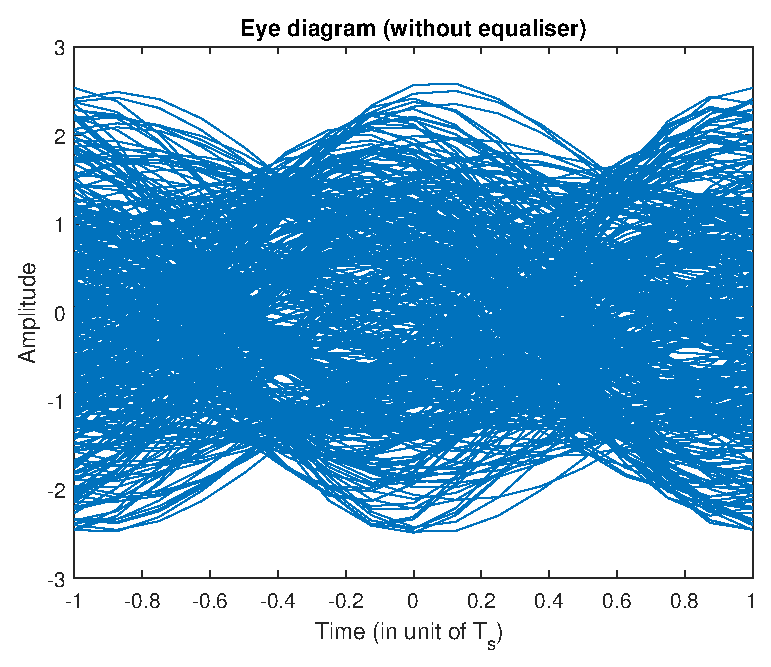
\includegraphics[width=0.8\textwidth]{plots/multipath_eye.eps}
    \caption{Eye diagram without equaliser\label{badeye}}
\end{figure}

\begin{figure}[H]
    \centering
    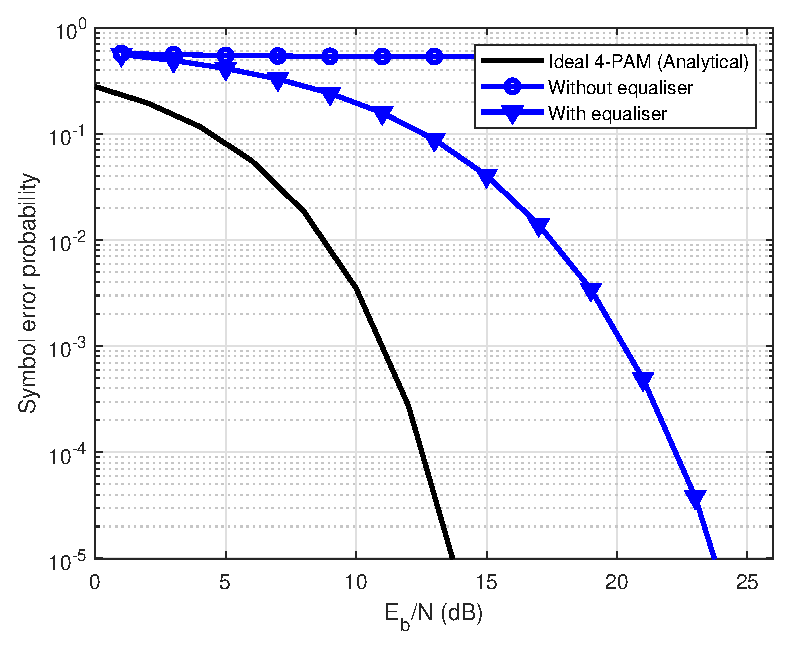
\includegraphics[width=0.8\textwidth]{plots/symbol_error_eq.eps}
    \caption{Symbol error probability with and without equaliser\label{eq_err}}
\end{figure}

\begin{figure}[H]
    \centering
    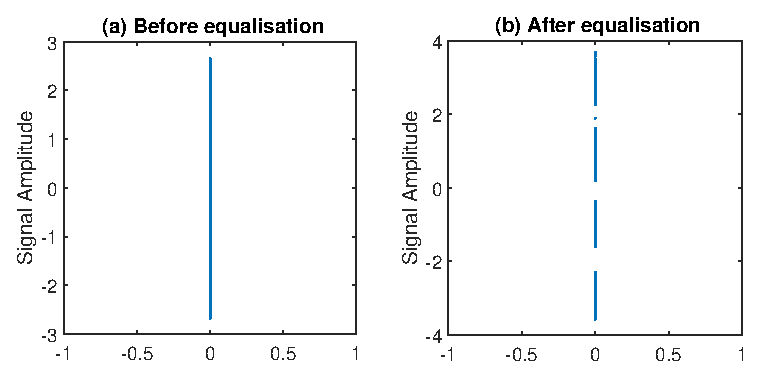
\includegraphics[width=0.8\textwidth]{plots/constellation_eq.eps}
    \caption{Signal amplitude levels (constellation) with and without
        equaliser\label{constellation}}
\end{figure}

\begin{figure}[H]
    \centering
    \includegraphics[width=0.8\textwidth]{plots/channel_impulse.eps}
    \caption{Impulse response of multipath channel}
\end{figure}

\subsection{Analysis}
Equalization can greatly improve the performance of a communication system.
Prior to use of an equalizer, the `eye' is completely closed as shown in
\Cref{badeye}. There is no margin over noise. After equalization, a larger
margin over noise is produced, meaning the eye is `open' and signals can be
decoded with an error rate less than 100\%. This difference can be shown in the
constellations in \Cref{constellation}, with gaps showing margin over noise only
appearing after equalization.

Due to there being zero margin over noise prior to equalization, the receiver is
effectively sampling nothing but ISI noise. Because of this, the error rate is a
flat 60\% for all SNRs, illustrated by the `without equalizer' plot in
\Cref{eq_err}.



\section{Lab Exercise}
\begin{figure}[H]
    \centering
    \includegraphics[width=0.8\textwidth]{scope.png}
    \caption{Oscilloscope output for signal generator \textbf{A}\label{scope}}
\end{figure}
\subsection{Steps required to generate image}
\begin{figure}[H]
    \centering
    \includegraphics[width=0.8\textwidth]{scope_setup.png}
    \caption{Experiment setup}
\end{figure}
These steps can be used to generate an eye diagram on a generic digital storage
oscilloscope:
\begin{enumerate}
    \item Connect the signal and clock outputs of the signal generator to two
          input channels of the oscilloscope.
    \item Set the trigger of the oscilloscope to use the clock channel.
    \item Adjust the trigger level to approximately half of the maximum
          amplitude of the clock signal, about 2.5V in this case. Any trigger
          level such that the refresh is only triggered on the edge of a pulse
          will work (ie. not above the max amplitude but not below the noise
          threshold of a clock `0' output).
    \item Adjust the horizontal scaling factor of the oscilloscope such that
          about three clock pulses are visible in the oscilloscope output
          window.
    \item Adjust the vertical scaling of both the signal and clock waveforms so
          main features are visible and large enough to measure using the volts
          per division and grid.
    \item Turn the persistence of the oscilloscope to maximum ($\infty$)
    \item If the image needs to be adjusted (scaled or horizontally offset), the
          persistence must be cleared.
\end{enumerate}

\subsection{Modulation type}
As shown in \Cref{scope}, the signal output shows four main levels at the eye
open instant. These are levels of voltage (signal \textit{amplitude}). Because
of this, the modulation type is 4-PAM.

\subsection{Signal characteristics}
\paragraph{Symbol rate}
The symbol rate is the frequency at which symbols are transmitted, which can be
found by the reciprocal of the time between clock pulses. Measured at 2.66KHz.
\paragraph{Error free sampling interval}
The error free sampling interval is the horizontal distance between the
left-most and right-most corners of the eye. In this interval, the signal has
settled in to one of the threshold regions for symbol decoding and will be
correctly decoded. Measured at 260us.
\paragraph{Margin over noise}
Noise margin is the voltage difference between a threshold (the horizontal axis
of the eye) and the maximum value of a noisy signal at the widest opening point
of the eye. If the signal were to be distorted by more than this margin, it
would cause a bit error even with if the sampling instant was chosen optimally.
Measured at 200mV.
\paragraph{Level crossing timing jitter}
Level crossing jitter is the variation in when signals cross the threshold
level. It shows the clock stability of the transmitter or phase distortion in
the transmission medium. Measured at 120us.

\subsection{Sensitivity of signal to timing error}
The error free sampling interval (260us) is a large proportion (approximately
70\%) of the entire symbol period (376us). Because of this, errors in timing
will be tolerated well, provided the timing error is not cumulative. If the
timing error is purely a phase error, a wide range of errors will be tolerated.
If the timing error is a sampling frequency error (ie. desynchronization of
local oscillators), the symbols will become corrupted as the RX sampling
oscillator moves out of the 260us window.

An eye diagram with a large error free sampling period may signify the signal
has not been band limited inside the bandwidth of the original TX pulse shape.
Since the measured signal exhibits this characteristic, it has not been band
limited.
\end{document}